\documentclass[11pt, a4paper]{book}

\usepackage{exsheets}
\SetupExSheets{counter-format=ch.qu}

\usepackage{epigraph}
\setlength{\epigraphwidth}{0.6\textwidth}
\setlength{\epigraphrule}{0pt}
\newcommand{\myopeningquote}{\smash{\raisebox{-0.25\height}{\llap{\scalebox{3}
				{\textcolor{silver}{``}}\,}}}}
\newcommand{\myclosingquote}{\raisebox{-0.86\height}{\scalebox{3}{\textcolor{silver}{”}}}}

\usepackage{sectsty}
\usepackage{titlesec}
\chapterfont{\color{rahmen}}
\subsectionfont{\color{rahmen}}
\subsubsectionfont{\color{rahmen}}
\titleformat{\section}
{\normalfont\Large\bfseries\color{rahmen}}{\textcolor{rahmen}\thesection}{1em}{}[\textcolor{rahmen}{\titlerule[0.1pt]}]

\patchcmd{\thebibliography}{\chapter*}{\section*}{}{}

\usepackage{afterpage}
\usepackage[inline]{enumitem}
\usepackage{cancel}
\usepackage{tabularx}
\usepackage{booktabs}
\usepackage{makecell}
\setcellgapes{4pt}

\usepackage{geometry}
\geometry{verbose,tmargin=2.5cm,bmargin=2.5cm,lmargin=2.5cm,rmargin=2.5cm,headheight=14pt}

\usepackage[most]{tcolorbox}
\newtcolorbox{attention}{breakable,enhanced,arc=2mm,colback=cream,colframe=goldenrod,leftrule=12mm,
	overlay={\node[anchor=north west,outer sep=2pt] at (frame.north west) {
\includegraphics[width=8mm]{figures/alert.png}}; }}
\newtcolorbox{curiosity}{breakable,enhanced,arc=2mm,colback=lime,colframe=green,leftrule=12mm,
	overlay={\node[anchor=north west,outer sep=2pt] at (frame.north west) {
\includegraphics[width=8mm]{figures/curiosity.png}}; }}
\newtcolorbox{finmarkets}{breakable,enhanced,arc=2mm,colback=sky,colframe=rahmen,leftrule=12mm,
	overlay={\node[anchor=north west,outer sep=2pt] at (frame.north west) {
\includegraphics[width=8mm]{figures/python_logo.png}}; }}

%\usepackage{amssymb}
\usepackage{amsfonts} % for expectation and other chars
\usepackage{bbm} % for indicator function
\usepackage{eurosym} % defines \euro

\usepackage{xcolor}
\definecolor{mandellightgreen}{rgb}{0.77, 0.82, 0.73}
\definecolor{mandelpantone}{rgb}{0.2, 0.11, 0.27}
\definecolor{ipython-frame}{RGB}{207, 207, 207}
\definecolor{ipython-bg}{RGB}{247, 247, 247}
\definecolor{ipython-red}{RGB}{186, 33, 33}
\definecolor{ipython-green}{RGB}{0, 128, 0}
\definecolor{ipython-cyan}{RGB}{64, 128, 128}
\definecolor{ipython-purple}{RGB}{170, 34, 255}
\definecolor{cream}{RGB}{255,229,153}
\definecolor{goldenrod}{RGB}{218,165,32}
\definecolor{sky}{RGB}{150, 195, 255}
\definecolor{rahmen}{RGB}{0,73,114}
\definecolor{ansi-red}{HTML}{E75C58}
\definecolor{ansi-green}{HTML}{00A250}
\definecolor{silver}{HTML}{C0C0C0}

\newcommand\Pdef{P_{\text{def}}}
\newcommand\Psur{P_{\text{sur}}}
\newcommand\corr{\text{Corr}}
%\newcommand\cov{\text{Cov}}
%\newcommand\var{\text{Var}}
\newcommand\std{\text{Std}}

\DeclareMathOperator{\var}{Var}
\DeclareMathOperator{\cov}{Cov}

\usepackage{hyperref}
\hypersetup{
	breaklinks=true,  % so long urls are correctly broken across lines
	colorlinks=true,
	urlcolor=rahmen,
	linkcolor=rahmen,
	citecolor=rahmen,
}
\hypersetup{linkcolor=rahmen}

\providecommand{\tightlist}{\setlength{\itemsep}{0pt}\setlength{\parskip}{0pt}}

\usepackage{subfig} %for subfloat

\usepackage{cprotect}
\lstdefinelanguage{iPython} {
	morekeywords={access,and,del,except,exec,in,is,lambda,not,or,raise},
	morekeywords=[2]{for,print,abs,all,any,basestring,bin,bool,bytearray,callable,chr,classmethod,cmp,compile,complex,delattr,dict,dir,divmod,enumerate,eval,execfile,file,filter,float,format,frozenset,getattr,globals,hasattr,hash,help,hex,id,input,int,isinstance,issubclass,iter,len,list,locals,long,map,max,memoryview,min,next,object,oct,open,ord,pow,property,range,reduce,reload,repr,reversed,round,set,setattr,slice,sorted,staticmethod,str,sum,super,tuple,type,unichr,unicode,vars,xrange,zip,apply,buffer,coerce,intern,elif,else,if,continue,break,while,class,def,return,try,except,import,finally,try,except,from,global,pass, True, False},
	sensitive=true,
	morecomment=[l]\#,
	morestring=[b]',
	morestring=[b]",
	moredelim=**[is][\color{black}]{@@}{@@},
	identifierstyle=\color{black}\footnotesize\ttfamily,
    commentstyle=\color{ipython-cyan}\footnotesize\itshape\ttfamily,
	stringstyle=\color{ipython-red}\footnotesize\ttfamily,
	keepspaces=true,
	showspaces=false,
    showstringspaces=false,
	rulecolor=\color{ipython-frame},
	frame=single,
	frameround={t}{t}{t}{t},
	framexleftmargin=6mm,
	numbers=left,
	numberstyle=\color{black},
	basicstyle=\footnotesize\ttfamily,
	keywordstyle=[2]\color{ipython-green}\bfseries\footnotesize\ttfamily, 
	keywordstyle=\color{ipython-purple}\bfseries\footnotesize\ttfamily,
	mathescape=true,
	escapeinside={*@}{@*}
}

\lstdefinelanguage{iOutput} {
	sensitive=true,
	identifierstyle=\color{black}\small\ttfamily,
	stringstyle=\color{ipython-red}\small\ttfamily,
	keepspaces=true,
	showspaces=false,
	showstringspaces=false,
	rulecolor=\color{ipython-frame},
	%frame=single,
	%frameround={t}{t}{t}{t},
	%backgroundcolor=\color{ipython-bg},
	basicstyle=\small\ttfamily,
	mathescape=true,
	escapeinside={*@}{@*}
}

\lstdefinestyle{mycpp}{language=C++,
	basicstyle=\small\ttfamily,
	showstringspaces=false,
	keywordstyle=\small\color{blue}\ttfamily,
	stringstyle=\small\color{red}\ttfamily,
	commentstyle=\small\color{green}\ttfamily,
	rulecolor=\color{ipython-frame},
	frame=single,
	frameround={t}{t}{t}{t},
	backgroundcolor=\color{ipython-bg},
	morecomment=[l][\color{magenta}]{\#}
}

\lstdefinestyle{attstyle}{
	backgroundcolor=\color{cream},
	rulecolor=\color{goldenrod}
}

\lstnewenvironment{attpython}[1][]{
	\lstset{language=iPython,style=attstyle,mathescape=true}
}{}

\lstnewenvironment{ipython}[1][]{\lstset{language=iPython,backgroundcolor=\color{ipython-bg}}}{}

\lstnewenvironment{ipythonnon}[1][]{\lstset{language=iPython,backgroundcolor=\color{ipython-bg},numbers=none,framexleftmargin=0mm}}{}

\lstnewenvironment{ipythonbox}[1][]{\lstset{language=iPython,numbers=none,framexleftmargin=0mm}}{}

\lstnewenvironment{ioutput}[1][]{\lstset{language=iOutput}}{}

\newcommand{\pythoncode}[1]{
    \lstinputlisting[language=iPython,backgroundcolor=\color{ipython-bg}]{#1}
}

\newcommand{\pythoncodenon}[1]{
    \lstinputlisting[language=iPython,numbers=none,backgroundcolor=\color{ipython-bg},framexleftmargin=0mm]{#1}
}

\newcommand{\pythoncodebox}[1]{
	\lstinputlisting[language=iPython,numbers=none,framexleftmargin=0mm]{#1}
}

\usepackage{fancyhdr}
\pagestyle{fancy}
%\renewcommand{\chaptermark}[1]{\markboth{\thechapter.\ #1}{}}
\renewcommand{\sectionmark}[1]{\markboth{\thesection.\ #1}{}}
\fancypagestyle{main}{
	\fancyhf{}
    \fancyhead[LO,RE]{\leftmark}
	\fancyhead[LE,RO]{\thepage}
	%\fancyfoot[C]{\thepage}
	\renewcommand{\headrulewidth}{0.4pt}
}

\SetupExSheets[solution]{print=false}

\begin{document}
\pagenumbering{gobble} 
\frontmatter
\pagestyle{empty}

\DeclareFixedFont{\titlefont}{T1}{ppl}{b}{n}{0.7in}
\DeclareFixedFont{\subtitlefont}{T1}{ppl}{b}{n}{0.4in}
\DeclareFixedFont{\authorfont}{T1}{ppl}{b}{n}{0.2in}

\afterpage{\restoregeometry}
\newgeometry{left=1in, right=1in,top=1in, bottom=0in}
%\pagecolor{mandelblue}\afterpage{\nopagecolor}

\newtcolorbox{mytransparentbox}[1][]{%
	coltext=white,
	arc=0pt,
	auto outer arc,
	enhanced jigsaw,
	opacityback=0.6,
	opacityframe=0.0,
	colback=mandellightgreen,
	width=1.2\paperwidth,
	boxrule=0pt,
	oversize=4cm,
	#1
}

\begin{tikzpicture}[overlay,remember picture]
	\node[rotate=0] at ([yshift=-14.8cm]current page.north)
	{\includegraphics[width=\paperwidth]{figures/copertina}};
\end{tikzpicture}

\thispagestyle{empty}

\vspace{10cm}
\begin{mytransparentbox}[height=8cm]
\begin{flushright}
	\color{mandelpantone}
	\vspace{0.5cm}
	\titlefont Numerical Recipes \\for Finance\\
	\vspace{0.5cm}
	\subtitlefont With Python Applications \\
	\vspace{1cm}
	\authorfont MATTEO SANI 
\end{flushright}
\end{mytransparentbox}

\restoregeometry


\thispagestyle{empty}
\cleardoublepage\null
\vspace*{\fill}
\begin{minipage}{0.25\textwidth}

\includegraphics[width=0.9\textwidth]{figures/by-nc-nd}
\end{minipage}
\begin{minipage}{0.75\textwidth}
Numerical Recipes for Finance with Python Applications © 2023 by Matteo Sani is licensed under CC BY-NC-ND 4.0. To view a copy of this license, visit \href{http://creativecommons.org/licenses/by-nc-nd/4.0}{http://creativecommons.org/licenses/by-nc-nd/4.0}.
\end{minipage}
\thispagestyle{empty}


\tableofcontents
\addtocontents{toc}{\protect\thispagestyle{empty}}

\mainmatter
\pagestyle{main}

\chapter{Introduction to \texttt{python}}
\label{introduction-to-python}

\section{Overview}
\texttt{Python} is one of the most widely used programming languages in the world, and it has been around for almost 30 years now~\cite{survey2021}.

First and foremost reason why \texttt{python} is much popular because it is highly productive as compared to other programming languages like \texttt{C++} and \texttt{java}. It is a much more concise and expressive language and requires less time, effort, and lines of code to perform the same operations.

This makes \texttt{python} a very easy-to-learn programming language even for beginners and newbies. It is also very famous for its simple programming syntax, code readability and English-like commands that make coding in \texttt{python} lot easier and efficient.
With \texttt{python}, the code looks very close to how humans think. For this purpose, it must abstract the details of the computer from you. Hence, it is slower than other “lower-level language” like \texttt{C}.

It has a good reputation in Data Science when combined with \texttt{numpy} and \texttt{pandas}. \texttt{Jupyter} as an interactive console has also contributed to making Python one of the most widely chosen languages for Data Science projects. 

Unfortunately it is a slow number cruncher because it was designed as a very high level loosely typed language. 
There were times when computer run-time used to be the main issue and the most expensive resource. But now, things have changed. Computer, servers and other hardware have become much much cheaper than ever and speed has become a less important factor. Today, development time matters more in most cases rather than execution speed. Reducing the time needed for each project saves companies tons of money.

As far as the execution speed or performance of the program is concerned, we can easily manage it by horizontal scaling, meaning that more servers can be used to reach that level of speed or performance.

In short, \texttt{python} is widely used even when it is somehow slower than other languages because:
\begin{itemize}
\tightlist
\item is more productive;
\item companies can optimize their most expensive resource: employees;
\item rich set of libraries and frameworks;
\item large community.
\end{itemize}

\begin{figure}[!ht]
\centering
\subfloat[Most used programming languages.\label{subfig-1:used}]{%
	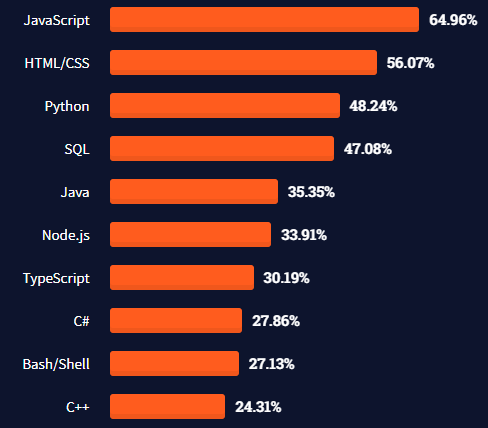
\includegraphics[width=0.5\textwidth]{figures/most_used_2021}
	}\\
\subfloat[Most loved and dreaded programming languages.\label{subfig-2:loved_dreaded}]{%
	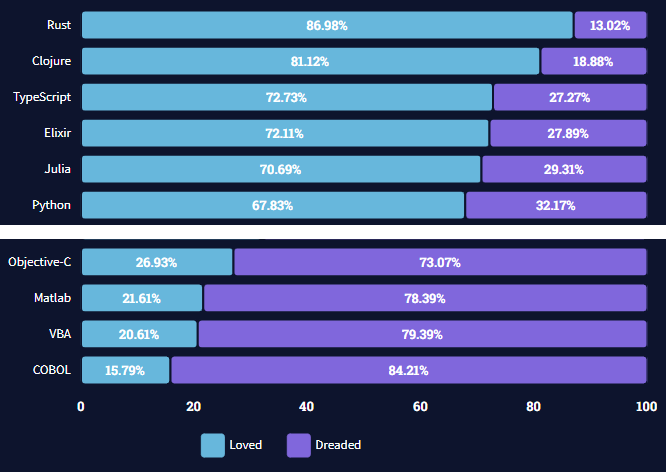
\includegraphics[width=0.7\textwidth]{figures/most_loved_dreaded_2021}
	}
\caption{Results from 2021 Stack Overflow survey.}
\label{fig:dummy}
\end{figure}

\subsection{Why \texttt{python}}

Assuming to have to simulate quantitative strategies for derivatives using plain statistics (no Machine Learning techniques involved), the typical step you have to take is to iterate a large number of times on quite big data sets (e.g. million of records data sets per asset).

It is then needed a programming language that could deal easily and without efforts with large data sets and was reasonably fast (do not consider for the moment integration with AI libraries).

Let's look at the possible alternatives to \texttt{python} for this typical endeavor.

\subsubsection{\texttt{R}}
\texttt{R} language has been the natural choice for doing statistics in the scientific community well before Data Science term was coined. While it is revolutionary and well suited to statistics, it is undoubtedly difficult to master and extremely inefficient in handling large data sets. 

Those are quite serious drawbacks, trading simulation usually requires large amounts of data, and if you need to start splitting it in advance or looking for alternative loading methods or simply the load process is complex it is worth to explore other options. 

This does not mean that \texttt{R} can not cope with it, it is just that it is not as easy and straightforward as for other languages. Data loading is an integral part of data analysis and it shall be provided out of the box.

\subsubsection{\texttt{C-C++}}
You can not be wrong with \texttt{C}. \texttt{C} is mature, it can do almost anything and it delivers very efficient code. \texttt{C} did not change substantially since its standard was formulated back in 1989. \texttt{C++} is also widely used and "extends" \texttt{C} with object-oriented paradigms.

The main problem with \texttt{C} is that it is "difficult" to do complex things with it. It shines for small algorithmic routines, and it is actually quite difficult to make it perform slow, but \emph{pointers} and their debugging can be challenging.
Usually while a project is getting bigger the timings and complexity to debugging it slowly but steadily grows.
Additionally, certain tasks which are trivial in other languages can be really challenging in \texttt{C}. 

\texttt{C/C++} language is widely used in High Frequency Trading (HFT) industry because it is a natural performer, but you must be ready to cope with longer projects that require skilled resources. It is the preferred choice when performance is paramount. 

\subsubsection{\texttt{Python} + \texttt{C}}
The logical to step to overcome \texttt{python} slowness is to replace its slow areas with \texttt{C}. 
The \texttt{C} routines when packed in \emph{shared libraries} can be invoked from \texttt{python} and this can be a win-win solution where you get the best of both worlds: speed from \texttt{C} and simplicity from \texttt{python}.

\subsubsection{\texttt{Fortran}}
\texttt{Fortran} is one of the oldest programming languages in service, \texttt{COBOL} aside. It was once the first choice for scientific and engineering analysis until the 90s and it has remained strong in computing demanding areas of the science.
\texttt{Fortran} is now a niche language but it still has an active community in many specialized fields such as high-energy physics, climate modeling, computational chemistry, structural engineering and molecular dynamics. Together with \texttt{C}, it is also the main programming language for super-computing. 

Modern \texttt{fortran} is quite easy to learn and master and often the algorithmic parts are easier to write than in \texttt{C}. \texttt{Fortran} also has some unique solutions to deal with array and structured data, which includes custom indexes, vector operations and simple ways to initialize variables and structures.

There are also some problems like bad integration of graphical tools and again debugging.  

\subsubsection{\texttt{Julia}}
\texttt{Julia} promises to deliver the simplicity of \texttt{python} with the speed of \texttt{C}.
The language is easy to learn and properly structured. The syntax is clear, it is not verbose and it is legible. Modules allow to adequately separate the code.

Certain aspects of the language were a bit puzzling at the beginning (i.e. mutable, variable sharing) but it is flexible enough to keep simpler tasks simple. Timestamp handling is pretty easy too, something which is relevant in this industry.
The overall times required to perform calculation are close to \texttt{C} since it compiles code in advance. The package installation service is also better incorporated than in \texttt{python} and it can be easily interfaced to it.

Using \texttt{julia} feels like you are an early adopter of a new technology and it might not be as stable and mature as other languages.

\section{What is \texttt{python} ?}
\label{what-is-python}

\texttt{Python} is a so called \emph{interpreted language}: it takes some code (a sequence of instructions), reads and executes it. This is different from other programming languages like \texttt{C} or \texttt{C++} which \emph{compile} code into a language that computers can understand directly (\emph{machine language}) (see Fig.~\ref{fig:compiled_vs_interpreted}).

\begin{figure}[htbp]
\centering
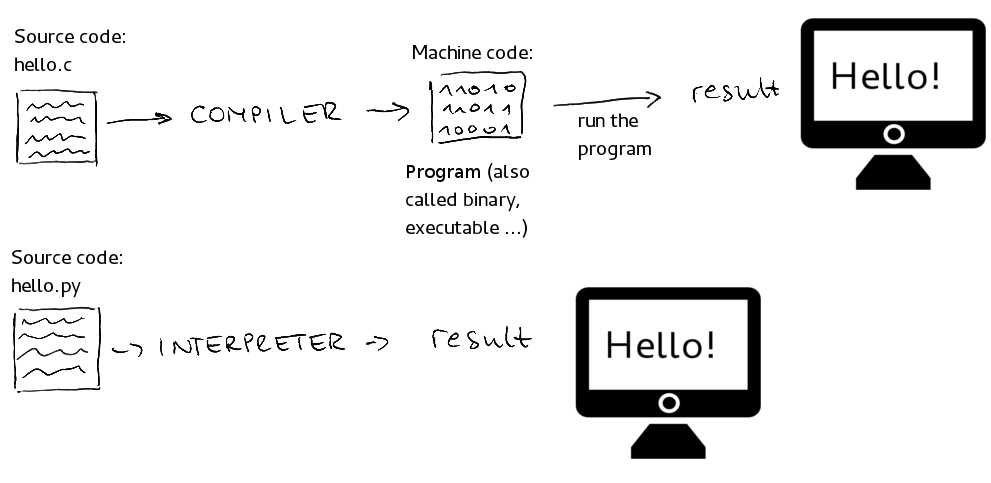
\includegraphics[width=0.7\linewidth]{figures/compiled_language}
\caption{Interpreted vs compiled language.}
\label{fig:compiled_vs_interpreted}
\end{figure}

As a result, \texttt{python} is essentially an \emph{interactive} programming language, which means you can program and see the results almost at the same time. This is very nice for a faster development since "compilation" time can be quite long (just to give an idea the compilation of our \texttt{C++} financial code takes more than one hour).
However there are drawbacks in term of performance, the \emph{translation} to machine language has to be done in real-time resulting in slower execution times (see Fig.~\ref{fig:compilation}).

\begin{figure}[htbp]
\centering
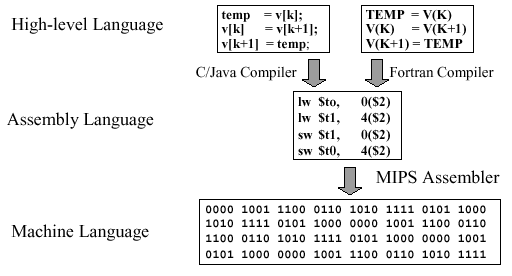
\includegraphics[width=0.5\linewidth]{figures/machine_language.png}
\caption{Human readable vs machine code}
\label{fig:compilation}
\end{figure}

In the next Chapters we'll take a quick tour of \texttt{python} and see the main features and characteristics of this programming language. Later on we will see how it can be useful to solve real-world financial problems.

First of all since \texttt{python}, as basically all programs, comes in different version and flavors we need to specify the particular one we are going to use~\cite{python_versions}.
The latest version (at the time I'm writing these pages) is \texttt{3.8.5}, however it is still not difficult to see older versions floating around (e.g. \texttt{2.7}).
This is because there are some big differences between \texttt{python 2.X} and \texttt{python 3.X} which prevent a sizable portion of \texttt{python 2} users to stick with it (consider that moving to \texttt{python 3} would require a large amount of work to adapt big projects).
In conclusion we will concentrate on \textbf{\texttt{python~3.X}}.

\section{\texttt{Python} Basics}
\label{python-basics}

Every language has \emph{keywords}, these are reserved words that have special meaning and tell the computer what to do. The most common one is \texttt{print}: it prints to screen whatever is specified between the parenthesis.
	
\begin{ipythonnon}
print ("Hello world !")
\end{ipythonnon}
\begin{ioutput}
Hello world !
\end{ioutput}
\begin{ipythonnon}
print ("Welcome")
print ("to")
print ("everybody")
\end{ipythonnon}
\begin{ioutput}
Welcome
to
everybody
\end{ioutput}

Good programming practice recommends to document the code you write (you will soon see that it is surprisingly easy to forget what you wanted to do in your code). In \texttt{python} you can add comments to code starting a line with a hash character (\#).

\begin{ipythonnon}
print ("Ciao") # this is a comment 
\end{ipythonnon}
\begin{ioutput}
Ciao
\end{ioutput}

\subsection{Variables}\label{variables}

If we want to really simplify what a program is and what it does, we may say that it is a series of instructions to be performed on various kind of data. Such data may be the name of a place, the height of a person or a series of prices taken by a trader. In programming, when we want to “label” a piece of information we give it a name and call it a variable, so we may say that a variable is a box which contains some kind of data.

More formally we can say that a variable is a computer memory location paired with a symbolic name, which contains some quantity of information referred to as a \emph{value} (e.g. a number, a string\ldots). 

A value is assigned to a variable with the equal operator (=) and printing a variable shows its content. 

\begin{figure}[htbp]
\centering
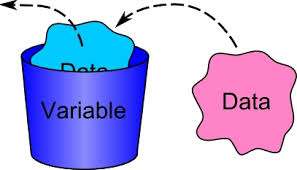
\includegraphics[width=0.35\linewidth]{figures/var1.jpeg}\\
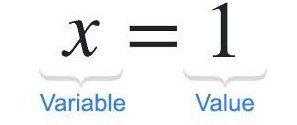
\includegraphics[width=0.35\linewidth]{figures/var2.jpeg}
\caption{Graphical representation of a variable.}
\end{figure}

\begin{ipythonnon}
x = 9 
print (x)
\end{ipythonnon}
\begin{ioutput}
9
\end{ioutput}
\begin{ipythonnon}
myphone = "MyFavourite Modile brand" 
print (myphone)
\end{ipythonnon}
\begin{ioutput}
MyFavourite Modile brand
\end{ioutput}

Another very useful keyword is \texttt{type}: it tells which kind of object is stored in a variable.

\begin{ipythonnon}
print (type(x))
print (type(myphone))
\end{ipythonnon}
\begin{ioutput}
<class 'int'>
<class 'str'>
\end{ioutput}

After their definitions \texttt{x} and \texttt{myphone} can be used as aliases for a number and a string and their content manipulated, for example:

\begin{ipythonnon}
print (x + 5)
\end{ipythonnon}
\begin{ioutput}
14
\end{ioutput}

There are rules that limit the variable naming possibilities, in particular they must:
\begin{itemize}
\tightlist
\item begin with a letter (\texttt{myphone}) or underscore (\texttt{\_myphone});
\item other characters can be letters, numbers or more underscores;
\item variable names are case-sensitive so \texttt{myphone} and \texttt{myPhone} are two distinct variables.
\end{itemize}

\textbf{Keywords, as said, are reserved words and as such cannot be used as variable names (e.g.~\texttt{print, type, for\ldots})}.

To use \textbf{good} variable names (and make your programs clearer and easier to read) always choose meaningful names instead of short names (i.e. \texttt{numberOfCakes} is much better than simply \texttt{n}), try to be consistent with your conventions (e.g.~choose once and for all between \texttt{number\_of\_cakes}, \texttt{numberofcakes} or \texttt{numberOfCakes}), usually begin a variable name with underscore (\_) only for a special case (will see later when this is necessary).

\subsection{Boolean Expressions}\label{boolean-expressions}

Boolean expressions evaluate to \texttt{True} or \texttt{False} only. This type
of expressions usually involve logical or comparison operators like \texttt{or}, \texttt{and}, $\geq$ (greater-than), $\leq$ (less-than)\ldots
The equal-to Boolean operator symbol is a double equal symbols (\texttt{==}), to not be confused with the assignment operator we have seen before made of a single equal symbol (\texttt{=}). With the first we compare two variables, with the second we associate a value to a variable.

Let's see some example. The following expression answers the question is 1 equal to 2:

\begin{ipythonnon}
1 == 2
\end{ipythonnon}
\begin{ioutput}
False
\end{ioutput}

Here another example using the not equal operator (\texttt{!=}):

\begin{ipythonnon}
1 != 2
\end{ipythonnon}
\begin{ioutput}
True
\end{ioutput}
\begin{ipythonnon}
2 < 2
\end{ipythonnon}
\begin{ioutput}
False
\end{ioutput}
\begin{ipythonnon}
2 <= 2 # in this case we allow the numbers to be equal too 
\end{ipythonnon}
\begin{ioutput}
True
\end{ioutput}
\begin{ipythonnon}
print (x)
15 <= x and x <= 20 # this expression could also be written as 15 <= x <= 20
\end{ipythonnon}
\begin{ioutput}
11
False
\end{ioutput}
\begin{ipythonnon}
15 <= x or x <= 20 
\end{ipythonnon}
\begin{ioutput}
True
\end{ioutput}
\begin{ipythonnon}
not (x > 20) # the not keyword negates the following expression 
\end{ipythonnon}
\begin{ioutput}
True
\end{ioutput}

\subsection{String Expressions}\label{string-expressions}

A string is a sequence of characters (letters, digits, spaces, punctuation\ldots). There are many operations that can be performed on strings, like for example concatenate (with \texttt{+} operator), truncate, replace characters\ldots

\begin{ipythonnon}
mystring = "some text with punctuation, spaces and digits 10" 
mystring.replace("s", "z")
\end{ipythonnon}
\begin{ioutput}
'zome text with punctuation, zpacez and digitz 10'
\end{ioutput}

\begin{ipythonnon}
"abc" + "def" # it is possible to concatenate strings with + 
\end{ipythonnon}
\begin{ioutput}
'abcdef'
\end{ioutput}

\begin{ipythonnon}
"The number " + 4 + " is my favorite number"
# this causes an error since we are trying to concatenate a string
# with a number so two different kind of objects
\end{ipythonnon}
\begin{ioutput} 
Traceback (most recent call last):
  File "<stdin>", line 1, in <module>
TypeError: must be str, not int
\end{ioutput}

This is the first time we make a mistake so that the \texttt{python} interpreter returns an error. We will discuss more deeply errors and their management in a later Section. 
For the moment it is enough to know that to avoid this particular error is possible to \textbf{cast} an object to a different type which means to convert an object to a different type. In this case we can \emph{force} the number four to be represented as a string with the \texttt{str()} function:

\begin{ipythonnon}
"The number " + str(4) + " is my favorite number"
\end{ipythonnon}
\begin{ioutput}
'The number 4 is my favorite number'
\end{ioutput}

\begin{ipythonnon}
print (type(3.4)) 
print (type(str(3.4)))
\end{ipythonnon}
\begin{ioutput}
<class 'float'>
<class 'str'>	
\end{ioutput}

In this simple case everything worked fine but type casting is not always possible: for example a number can be converted to a string (e.g. from the integer 4 to the actual symbol "4") but the opposite is not possible (e.g. cannot convert the string "matteo" to a meaningful number). In this second case we can try to use the function \texttt{int()} to convert a string to an integer.

\begin{ipythonnon}
int("matteo")
\end{ipythonnon}
\begin{ioutput}
Traceback (most recent call last):
  File "<stdin>", line 1, in <module>
ValueError: invalid literal for int() with base 10: 'matteo'
\end{ioutput}

\begin{ipythonnon}
int("4") 
\end{ipythonnon}
\begin{ioutput}
4
\end{ioutput}

\subsubsection{Pretty String Formatting}
In order to get prettier strings than those obtained just concatenating with the + operator, \texttt{python} allows to format text using the following syntax: \texttt{f"text \{var1\} other text \{var2\}"}.
This is not just a mannerism, for example we will see that it may be very useful to represent prices with the correct number of significant digits.

Using optional characters inside the curly brackets can determine the resulting format, for example\texttt{f"\{var:.1f\}"} means that this variable is a float number and that has to be printed with only one digit only after the decimal separator. 

\begin{ipythonnon}
c = 299792.458
print (f"The speed of light is about {c:.1f} km/s")	
\end{ipythonnon}
\begin{ioutput}
The speed of light is about 299792.5 km/s
\end{ioutput}

In addition to rounding formatted string can handle 0-padding of numbers, left or right alignment and so on. For a complete list of the available features please refer to \href{https://docs.python.org/3/tutorial/inputoutput.html}{Input and Output}.

\subsection{Mathematical Expressions}\label{mathematical-expressions}

Below few examples of the basic mathematical expressions available in \texttt{python}.

\begin{ipythonnon}
print (1 + 2)	
\end{ipythonnon}
\begin{ioutput}
3
\end{ioutput}

\begin{ipythonnon}
print (40 - 5)	
\end{ipythonnon}
\begin{ioutput}
35
\end{ioutput}

\begin{ipythonnon}
print (x * 20) # remember that x is equal to 9
\end{ipythonnon}
\begin{ioutput}
180	
\end{ioutput}

\begin{ipythonnon}
print (x / 4)
\end{ipythonnon}
\begin{ioutput}
2.25
\end{ioutput}

\begin{ipythonnon}
print (type(2.25))
\end{ipythonnon}
\begin{ioutput}
<class 'float'>	
\end{ioutput}

\begin{ipythonnon}
x // 4 # integer division, result will be truncated (no rounding)
       # 11 / 3 = 3.66666, 11 // 3 = 3
\end{ipythonnon}
\begin{ioutput}
2
\end{ioutput}

\begin{ipythonnon}
y = 3
print (x**y) # x to the power of y 	
\end{ipythonnon}
\begin{ioutput}
729
\end{ioutput}

\begin{ipythonnon}
print (3*x + y)	
\end{ipythonnon}
\begin{ioutput}
36	
\end{ioutput}

As an example of variable manipulation let's try to increment \texttt{x} by 1 and save the result again in \texttt{x}.

\begin{ipythonnon}
print (x)
x = x + 1
print (x)	
\end{ipythonnon}
\begin{ioutput}
15
16
\end{ioutput}

Sometimes the increment of a variable plus the assignment to the same variable is written with a more compact syntax \texttt{x += 1} (this is also true for other operators e.g. \texttt{x *= 2}).

More complex mathematical functions are not directly available, let's see for example the logarithm:

\begin{ipythonnon}
log(3)
\end{ipythonnon}
\begin{ioutput}
Traceback (most recent call last):
  File "<stdin>", line 1, in <module>
NameError: name 'log' is not defined
\end{ioutput}

\subsection{Type Hints}

In Python, \textit{type hints} were introduced to bring clarity, safety, and documentation to code without sacrificing the language's flexible nature. 

Because Python is historically dynamically typed—meaning it does not naturally force you to declare whether a piece of data is a number, text, or a list—type signatures act as explicit labels attached to functions. They state upfront what kind of data a function expects to receive and what kind it will return. 

Although Python itself does not strictly enforce these labels while the program is running, typing signatures serve as clear documentation for humans and allow modern code editors to automatically detect potential errors before the program is ever executed.

\section{Modules}\label{modules}

One very important feature of each language is the ability to reuse code among different programs, e.g. imagine how awful would be if you had to re-implement every time you need it a function to compute the logarithm.
Usually there are mechanisms that allow to collect useful routines in \emph{packages} (or \emph{libraries}, or \emph{modules}) so that later they can be called and used by any program may need them.

These collections of utilities in \texttt{python} are called \emph{modules} and each installation of this language brings with it a standard set of them. If you need more functionality, you can download more modules from the web (there are zillions out there~\cite{modules}, see Fig.~\ref{fig:fancy_module}) or if you are not satisfied with what you found you can write your own (which is one of the goals of this course).

Some examples of useful modules we are going to use are:

\begin{itemize}
\tightlist
\item Numpy - which provides matrix algebra functionality and much more;
\item Scipy - which provides a whole series of scientific computing
  functions;
\item Pandas - which provides tools for manipulating time series or data-set
  in general;
\item Matplotlib - for plotting graphs;
\item Jupyter - for notebooks like the one used in classroom.
\end{itemize}

\begin{figure}
\centering
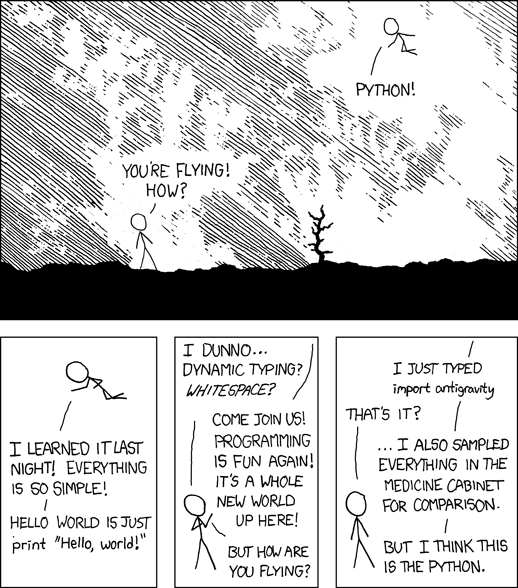
\includegraphics[width=0.5\linewidth]{figures/python.png}
\caption{\texttt{Python} has many modules for download on the web\ldots}
\label{fig:fancy_module}
\end{figure}

In Chapters~\ref{sec:datetime} and~\ref{sec:datamanip} we take a closer look at three modules which are particularly useful in financial analysis.

Notice that not all the modules are installed in your system with a standard \texttt{python} installation. In case you want to use one that is not available you can get it using the \texttt{pip} utility
\begin{ioutput}
pip install tensorflow
\end{ioutput}
Optionally it is possible to specify the exact version of the package that is needed like this
\begin{ioutput}
pip install tensorflow==3.0.1
\end{ioutput}
The command \texttt{pip} offers other useful options like to list the current installed packages
\begin{ioutput}
pip list
\end{ioutput}
Saving the output of the previous command to a file allows to later install at once all the listed packages to replicate a particular \texttt{python} environment

\begin{ioutput}
pip install -r pkg_list.txt
\end{ioutput}

Note that if you want to install a package in \texttt{Colab} just prepend an exclamation mark to the previous commands. 

In order to load a module in a \texttt{python} program you have to use the \texttt{import} keyword.
If a module name is long or awkward it is possible to define an alias with \texttt{import matplotlib.pyplot as plt}. To inspect a module, to understand which are its functionalities, it can be used either \texttt{help} and \texttt{dir} keywords: the first writes a help message which usually describes the functionalities of the module, the latter systematically lists all the available functions of a module.
\textbf{In order to access a function of a module you have to use the dot (\texttt{.}) operator: \texttt{module-name.function-name}.}

The \texttt{math} module implements the most common mathematical functions, let's see an example. 

\begin{ipythonnon}
import math
dir(math)
\end{ipythonnon}
\begin{ioutput}
['\_\_doc\_\_',
 '\_\_loader\_\_',
 '\_\_name\_\_',
 '\_\_package\_\_',
 '\_\_spec\_\_',
 'acos',
 'acosh',
 'asin',
 'asinh',
 'atan',
 'atan2',
 'atanh',
 ...
\end{ioutput}

\begin{ipythonnon}
help(math)
\end{ipythonnon}
\begin{ioutput}
Help on module math:

NAME
math

MODULE REFERENCE
https://docs.python.org/3.6/library/math

The following documentation is automatically generated from the Python
source files.  It may be incomplete, incorrect or include features that
are considered implementation detail and may vary between Python
implementations.  When in doubt, consult the module reference at the
location listed above.

DESCRIPTION
This module is always available.  It provides access to the
mathematical functions defined by the C standard.

FUNCTIONS
acos(...)
acos(x)

Return the arc cosine (measured in radians) of x.
...
\end{ioutput}

\begin{ipythonnon}
print (math.log(3))
\end{ipythonnon}
\begin{ioutput}
1.0986122886681098	
\end{ioutput}

\begin{ipythonnon}
print (math.exp(3))
\end{ipythonnon}
\begin{ioutput}
20.085536923187668	
\end{ioutput}

\begin{ipythonnon}
print (type(math.log)) # yet another type: builtin function
print (type(math.log(3)))
\end{ipythonnon}
\begin{ioutput}
<class 'builtin\_function\_or\_method'>
<class 'float'>	
\end{ioutput}

If you want to avoid to type \texttt{math.} every time you compute a logarithm or an exponential, it is possible to import only the needed functions from the module using the following syntax:

\begin{ipythonnon}
from math import log, exp

print (log(3))
print (exp(3))
\end{ipythonnon}
\begin{ioutput}
1.0986122886681098
20.085536923187668	
\end{ioutput}

As an example let's compute the interest rate $r$ that produces a return $R$ of 11000 EUR when investing 10000 EUR for 2 years:
\begin{equation*}
R = N\mathrm{e}^{r\tau} \implies r = \frac{1}{\tau} \mathrm{log}(\frac{R}{N})
\end{equation*}

\begin{ipythonnon}
rate = (1/2)*log(11000/10000)
print (rate)
\end{ipythonnon}
\begin{ioutput}
0.04765508990216247	
\end{ioutput}

\subsection{\texttt{finmarkets} Module}

Throughout this lectures many \texttt{python} financial applications will be reviewed. All code has been collected for simplicity into a \texttt{python} module called \texttt{finmarkets}. 

The module is currently in the \emph{test} repository of PyPi, the official collection of \texttt{python} modules. To install it in your working area you can still use \texttt{pip} but an additional option is needed 
\begin{ioutput}
pip install --index-url https://test.pypi.org/simple finmarkets
\end{ioutput}
	
Later you can access the code like all the other modules

\begin{ipythonnon}
from finmarkets import DiscountCurve
\end{ipythonnon}

\section{Indented Blocks and Conditionals}
\label{indented-blocks-and-the-ttifelse-statement}

Unlike other languages which uses parenthesis to isolate blocks of code \texttt{python} uses \emph{indentation}. A first example of this peculiarity is given by conditional statements (i.e. \texttt{if/elif/else}). Such commands allow to dynamically run different blocks of code based on conditions. For example in the following we print different statements according to the value of \texttt{x}, note that the block of code to be run according each condition is shifted (i.e. indented) with respect to the rest of the code:

\begin{ipythonnon}
print (x)
if x == 1:
	print ("This will not be printed")
elif x == 15:
	print ("This will not be printed either")
else:
	print ("This *will* be printed")
\end{ipythonnon}
\begin{ioutput}
16
This *will* be printed	
\end{ioutput}

If by mistake the indentation of a block is missing an exception is raised:

\begin{ipythonnon}
if x == 1:
    print ("This will not be printed")
elif x == 15:
    print ("This will not be printed either")
else:
   print ("This *will* be printed")
\end{ipythonnon}
\begin{ioutput}
  File "<stdin>", line 6
    print ("This will not be printed")
        ^
IndentationError: expected an indented block
\end{ioutput}

Below another example:
\begin{ipythonnon}
if x != 1:
    print ("x does not equal 1")
\end{ipythonnon}
\begin{ioutput}
x does not equal to 1	
\end{ioutput}

Just for comparison this is the same code written in \texttt{C++}:

\begin{lstlisting}[style=mycpp]
if (x == 1) {
 std::cout << "This will not be printed" << std::endl;
} else if (x == 15) {
     std::cout << "This will not be printed either" << std::endl;
} else {
   std::cout << "This *will* be printed" << std::endl;
}
\end{lstlisting}

Notice how indentation doesn't matter at all here since the blocks are enclosed and defined by the brackets.

\section{Loops}\label{loops}

Another very important feature of a language is the ability to repeatedly run the same block of code many times. This is called looping and in \texttt{python} can be done with \texttt{for} or \texttt{while} keywords.

\subsection{\texttt{for}}\label{for}

In a \texttt{for} loop we specify the set (or interval) over which we want to loop and a variable will assume all the values in that set (or interval). For example let's assume we want to print all the numbers between 25 and 30 (excluded) 

\begin{ipythonnon}
for i in range(25, 30):
    print (i)	
\end{ipythonnon}
\begin{ioutput}
25
26
27
28
29	
\end{ioutput}
\noindent
where the keyword \texttt{range} returns the list of integers between the specified limits, if the first limit is not specified 0 is assumed.
At each cycle of the loop the variable \texttt{i} takes one of the values between 25 and 29. 

With \texttt{range} it is also possible to specify the step, so that the loop can jump every 2 units or to go in descending order:

\begin{ipythonnon}
for i in range(30, 25, -1):
    print (i)	
\end{ipythonnon}
\begin{ioutput}
30
29
28
27
26	
\end{ioutput}

If it is needed to skip values in the loop the \texttt{continue} keyword can be used; in the code below 5 is actually not printed since it has been skipped by the condition executing \texttt{continue}:

\begin{ipythonnon}
for i in range(10):
    if i == 5:
        continue
    print (i)	
\end{ipythonnon}
\begin{ioutput}
0
1
2
3
4
6
7
8
9	
\end{ioutput}

Instead of using \texttt{range} it is possible to specify directly the set of looping values:

\begin{ipythonnon}
for i in (4, 6, 10, 20):
    print (i)	
\end{ipythonnon}
\begin{ioutput}
4
6
10
20	
\end{ioutput}

Finally looping on a string actually means to loop on each single character:
 
\begin{ipythonnon}
phrase = "how to loop over a string"
for c in phrase:
    print(c) 	
\end{ipythonnon}
\begin{ioutput}
h
o
w

t
o
...
\end{ioutput}
 
\subsection{\texttt{while}}\label{while}

The \texttt{while} statement repeats the same block of code until a condition is met. For example in the following code, the block is run until \texttt{x} squared is less than 50. At the beginning \texttt{x=1} and at each iteration we increment it by 1 "while" the condition is \texttt{True} (it should stop when \texttt{x}$> 7$ because it is the last squared lower than 50):

\begin{ipythonnon}
x = 1
while x**2 < 50:
    print (x)
    x += 1	
\end{ipythonnon}
\begin{ioutput}
1
2
3
4
5
6
7	
\end{ioutput}

It is possible to exit prematurely from a \texttt{while} loop using the \texttt{break} keyword. In this case the while-condition is simply \texttt{True} so the code would run forever unless we set an exit strategy.

\begin{ipythonnon}
x = 1
while True:
    if x**2 > 50:
        break
    print (x)
    x += 1	
\end{ipythonnon}
\begin{ioutput}
1
2
3
4
5
6
7	
\end{ioutput}

\section{Errors and Exceptions}
In the previous Sections we have already found a couple of examples with errors. Here we are going to look deeply what they are and how can be managed. There are (at least) two distinguishable kinds of errors:  \emph{syntax errors} and \emph{exceptions}.

\subsection{Syntax Errors}
Syntax errors are perhaps the most common kind of complaint you get while you are still learning \texttt{python}.

\begin{ipythonnon}
while True
    print ("Hello world")
\end{ipythonnon}
\begin{ioutput}
  File "<stdin>", line 1
    while True print('Hello world')
               ^
SyntaxError: invalid syntax
\end{ioutput}

The parser repeats the offending line and displays a little "arrow" pointing at the earliest point in the line where the error was detected. The error is caused by the token preceding the arrow: in the example, the error is detected at the function \texttt{print()}, since a colon (\texttt{:}) is missing before it. File name and line number are printed so you know where to look in case the input came from a script.

\subsection{Exceptions}
Even if a statement or expression is syntactically correct, it may cause an error when an attempt is made to execute it. Errors detected during execution are called exceptions and are not unconditionally fatal. Most exceptions are not handled by programs and result in error messages as shown here:

\begin{ipythonnon}
10 * (1/0)
\end{ipythonnon}
\begin{ioutput}
Traceback (most recent call last):
  File "<stdin>", line 1, in <module>
ZeroDivisionError: division by zero
\end{ioutput}

\begin{ipythonnon}
4 + spam*3
\end{ipythonnon}
\begin{ioutput}
Traceback (most recent call last):
  File "<stdin>", line 1, in <module>
NameError: name 'spam' is not defined
\end{ioutput}

\begin{ipythonnon}
'2' + 2
\end{ipythonnon}
\begin{ioutput}
Traceback (most recent call last):
  File "<stdin>", line 1, in <module>
TypeError: must be str, not int
\end{ioutput}

The last line of the error message indicates what happened. Exceptions come in different types, and the type is printed as part of the message: the types in the example are \texttt{ZeroDivisionError}, \texttt{NameError} and \texttt{TypeError}. The string printed as the exception type is the name of the exception that occurred. The rest of the line provides detail based on the type of exception and what caused it.

The preceding part of the error message shows the context where the exception occurred, in the form of a stack traceback listing source lines.

\subsection{Handling Exceptions}
It is possible to write programs that handle selected exceptions. Look at the following example, which asks the user for input until a valid integer has been entered, but allows the user to interrupt the program (e.g. using Control-C); note that a user-generated interruption is signaled by raising the \texttt{KeyboardInterrupt} exception.

\begin{ipythonnon}
while True: 
    try:
        x = int(input("Please enter a number: ")) 
        break
    except ValueError:
        print("Oops! That was no valid number. Try again...")
\end{ipythonnon}
\begin{ioutput}
Please enter a number: pippo
Oops!  That was no valid number.  Try again...

Please enter a number:
\end{ioutput}

The \texttt{try} statement works as follows: first, the try clause is executed. If no exception occurs, the except clause is skipped and execution of the \texttt{try} statement is finished.

If an exception occurs during execution of the try clause, the rest of the clause is skipped. Then if its type matches the exception named after the \texttt{except} keyword, the corresponding except clause is executed, and then execution continues after the \texttt{try} statement.

If an exception occurs which does not match the exception named in the except clause, it is passed on to outer \texttt{try} statements; if no handler is found, it is an un-handled exception and execution stops with a message as shown above.

A \texttt{try} statement may have more than one except clause, to specify handlers for different exceptions. At most one handler will be executed. Handlers only handle exceptions that occur in the corresponding try clause, not in other handlers of the same \texttt{try} statement.

\begin{ipythonnon}
except RuntimeError, TypeError, NameError:
    pass	
\end{ipythonnon}

The last except clause may omit the exception name(s), to serve as a wildcard. Use this with extreme caution, since it is easy to mask a real programming error in this way! 

\begin{ipythonnon}
import sys 

try:
    with open('myfile.txt') as f: 
        s = f.readline()
        i = int(s.strip()) 
except OSError as err:
    print(f"OS error: {err}") 
except ValueError:
    print("Could not convert data to an integer.") 
except:
    print("Unexpected error:", sys.exc_info()[0])
\end{ipythonnon}
\begin{ioutput}
OS error: [Errno 2] No such file or directory: 'myfile.txt'	
\end{ioutput}

\section{Assertions}
\texttt{Python} has a useful command called \texttt{assert} which can be used for checking that a given condition is satisfied, and it raises an exception if this is not true. This is clearly very important when debugging some code, it helps in searching for mistakes in the logic of an algorithm.

Below few examples of its usage. The following line does not cause an error, in fact it does nothing since 1 is lower than 2, hence the condition is met:

\lstinline[language=iPython]|assert 1 < 2|

\noindent
The next one instead causes an error (the condition is evaluated to false): 

\lstinline[language=iPython]|assert 1 > 2|

\noindent
\texttt{assert} can take a second optional argument with a message to display in case of failure.

\lstinline[language=iPython]|assert 1 > 2, "Two is greater than one"|

\section*{Exercises}
\begin{question}
What is the built-in function that \(\tt{python}\) uses to iterate over a number sequence ? Write an example that uses it.
\end{question}

\cprotEnv \begin{solution}
The built-in function used to iterate over a sequence of numbers is \(\tt{range}\). It returns a sequence of numbers taking three parameters that represents respectively the lower boundary of the sequence, the upper boundary of the sequence and the step. Note that the upper boundary is excluded from the sequence.

\begin{ipython}
for i in range(10, 20, 2):
    print (i)
\end{ipython}
\begin{ioutput}
10
12
14
16
18
\end{ioutput}
If just one parameter is passed the default lower boundary is 0 and the step is 1. 
\begin{ipython}
for i in range(5):
    print (i)
\end{ipython}
\begin{ioutput}    
0
1
2
3
4
\end{ioutput}
\end{solution}

\begin{question}
What is a string in \(\tt{python}\) ? Declare one string variable and try to manipulate it (concatenate, make uppercase, capitalize, replace characters, split...).
\end{question}

\cprotEnv \begin{solution}
A string is simply a sequence of characters.

\begin{ipython}
aString = "this is a string"
  
aString = aString + ", just an example"
print(aString)
\end{ipython}
\begin{ioutput}
'this is a string, just an example'
\end{ioutput}
\begin{ipython}
print(aString.upper())
\end{ipython}
\begin{ioutput}
'THIS IS A STRING, JUST AN EXAMPLE'
\end{ioutput}
\begin{ipython}
print(aString.capitalize())
\end{ipython}
\begin{ioutput}
'This is a string, just an example'
\end{ioutput}
\begin{ipython}
print(aString.replace("just an", "for"))
\end{ipython}
\begin{ioutput}
'this is a string, for example'
\end{ioutput}
\begin{ipython}
print(aString.split(","))
\end{ipython}
\begin{ioutput}
['this is a string', ' just an example']
\end{ioutput}
\begin{ipython}
if aString.endswith("example"):
    print("This string is really an example.")
else:
    print("This string is not an example.")
\end{ipython}
\begin{ioutput}
'This string is really an example.'
\end{ioutput}
\end{solution}

\begin{question}
What does the continue do in \(\tt{python}\) ? Show an example of its usage printing all the odd numbers between 0 and 10.
\end{question}

\cprotEnv \begin{solution}
\(\tt{continue}\) is used to skip cycles in for loops. Note that \% is the module operator, it returns the reminder of a division.

\begin{ipython}
for i in range(10):
    if i%2 == 0:
        continue
    else:
        print(i)
\end{ipython}
\begin{ioutput}    
1
3
5
7
9
\end{ioutput}
\end{solution}

\begin{question}
When should you use the break in \(\tt{python}\) ? Show an example of its usage.
\end{question}

\cprotEnv \begin{solution}
\(\tt{break}\) is the command used to interrupt a while loop even if the while condition is still satisfied.

\begin{ipython}
i = 0
while i < 11:
    if (i/2) > 3:
        break
    print(i)
    i += 1 
\end{ipython}
\begin{ioutput}    
0
1
2
3
4
5
6
\end{ioutput}
\end{solution}

\begin{question}
Which \(\tt{python}\) function will you use to convert a number to a string ? Show an example.
\end{question}

\cprotEnv \begin{solution}
\(\tt{str()}\) is the correct function to use in order to cast a number to a string.

\begin{ipython}
x = 2.34
print(f"This {x} is of type {type(x)}")
print(f"This {str(x)} is of type {type(str(x))}")
\end{ipython}
\begin{ioutput}    
This 2.34 is of type <class 'float'>
This 2.34 is of type <class 'str'>
\end{ioutput}
\end{solution}

\begin{question}
Import the math module and compute the logarithm of 2.09, the exponential of 1.57 and the area of a circle of radius 6 cm (circle area = $\pi \cdot r^2$).
\end{question}

\cprotEnv \begin{solution}
\begin{ipython}
from numpy import log, exp

print (f"log(2.09) = {log(2.09)}")
print (f"exp(1.57) = {exp(1.57)}")
print (f"area of a circle (R=6cm) is about {math.pi*6*6} cm2")
\end{ipython}
\begin{ioutput}    
log(2.09) = 0.7371640659767196
exp(1.57) = 4.806648193775178
area of circle (R=6cm) is about 113.10 cm2
\end{ioutput}
\end{solution}

\cprotEnv \begin{question}
\label{ex:BS1}
Given the following variables write out the Black Scholes formula and save the value of a call in a variable named `call\_price' and the value of a put in a variable named `put\_price'.

\begin{ipython}
S_t = 800.0 # spot price of the underlying
K = 600.0 # strike price
vol = 0.25 # volatility
r = 0.01 # interest rate
ttm = 0.5 # time to maturity, in years
\end{ipython}
\textbf{Hint:} remember that there are many modules available in \texttt{python} that let you save a lot of time. In this case we need the cumulative distribution function of the standard normal distribution which can be found in \texttt{scipy.stats} module, the name of the function is \texttt{norm}.
\end{question}

\cprotEnv \begin{solution}
The BS equation for the price of a call is:

\[ C(S, t) = S_tN(d_1)-Ke^{-r(T-t)}N(d_2) \]

where
\begin{itemize}
\item \(S_t\) is the spot price of the underlying
\item \(K\) is the strike price
\item \(r\) is the risk-free interest rate (expressed in terms of continuous compounding)
\item \(N(\cdot)\) is the cumulative distribution function of the standard normal distribution
\item \(T - t\) is the time to maturity
\item \(\sigma\) is the volatility of the underlying
\end{itemize}

\[\begin{split}
d_1 & = \cfrac{\mathrm{ln}(\cfrac{S_t}{K}) + (r + \cfrac{1}{2}\sigma^{2})(T-t)}{\sigma\sqrt{T-t}}\\ \\
d_2 & = d_1 - \sigma\sqrt{T-t}\\
\end{split}\]

\begin{ipython}
from math import log, exp, sqrt
# You'll need the Gaussian cumulative distribution function 
from scipy.stats import norm

S_t = 800.0 
ttm = 0.5
K = 600.0 
vol = 0.25 
r = 0.01

d1_num = (log(S_t/K)+(r+0.5*pow(vol, 2))*ttm) 
d1_den = vol*sqrt(ttm)
d1 = d1_num /d1_den
d2 = d1 - d1_den

call_price = S_t * norm.cdf(d1) - K * exp(-r*ttm)*norm.cdf(d2)
put_price = - S_t * norm.cdf(-d1) + K * exp(-r*ttm)*norm.cdf(-d2)
print (f"{call_price:.3f} {put_price:.3f}") 
\end{ipython}
\begin{ioutput}    
205.472 2.480
\end{ioutput}
\end{solution}

 % da riguardare
\chapter{Data Containers}
\label{sec:datacontainer}

In this Chapter the container types available in \texttt{python} are reviewed.

\section{Lists}
\label{lists}

A list in \texttt{python} is a container that is a \emph{mutable}, ordered sequence of elements. Each element or value that is inside of a list is called an \emph{item}. Each item can be accessed using square brackets notation, \texttt{alist[index]}, where \texttt{index} is the position of the item in the list.
Note that, list indexing is zero-based so the first element has index 0 actually. A list is considered mutable since you can add, remove or update the items in it. Ordered instead means that items are kept in the same order they have been added to. Lists can be created by enclosing in square brackets the comma-separated list of the items or using the \texttt{list()} operator.

\begin{ipython}
mylist = list([21, 32, 15])
mylist = [21, 32, 15]

print(mylist)
print (type(mylist))
\end{ipython}
\begin{ioutput}
[21, 32, 15]
<class 'list'>
\end{ioutput}

\begin{ipython}
print (mylist[0])
\end{ipython}
\begin{ioutput}
21
\end{ioutput}

If you have a list of lists (i.e. a 2-dimensional list) you can use the square brackets multiple times to access the inner elements:
\begin{ipython}
alist = [[1,2], [3,4], [5,6]]
print (alist[1][1]) # first [1] returns [3,4], second returns 4                 
\end{ipython}  

The number of elements in a list is counted using the function \texttt{len()}:
\begin{ipython}
print(len(mylist))
\end{ipython}
\begin{ioutput}
3
\end{ioutput}

Looping on list items can be achieved in two ways: using directly the list or by index:

\begin{ipython}
print ("Loop using the list itself:")
for i in mylist:
    print (i)
\end{ipython}
\begin{ioutput}
Loop using the list itself:
21
32
15
\end{ioutput}
\begin{ipython}
print ("Loop by index:")
for i in range(len(mylist)): # len returns number of items in the list
    print (i)
\end{ipython}
\begin{ioutput}
Loop by index:
21
32
15
\end{ioutput}

With the \texttt{enumerate} function is actually possible to do both at the same time since it returns two values, the index of the item and its value, so in the example below, \texttt{i} will take the item indices while \texttt{item} the item value itself:

\begin{ipython}
for i, item in enumerate(mylist):
    print (i, item)
\end{ipython}
\begin{ioutput}
0 21
1 74
2 85
3 15
4 188
\end{ioutput}

Since a list is mutable its items can be changed dynamically:

\begin{ipython}
mylist[1] = 74 # we can change list items since it's *mutable*
print (mylist)
\end{ipython}
\begin{ioutput}
[21, 74, 15]
\end{ioutput}

With \texttt{append} an item is added at the end, while with \texttt{insert} an item can be added in a specified position:

\begin{ipython}
mylist.append(188) # append add an item at the end of the list
print (mylist)
\end{ipython}
\begin{ioutput}
[21, 74, 15, 188]
\end{ioutput}
\begin{ipython}
mylist.insert(2, 85) # insert an item in the desired position
                     # (2 in this example)
print (mylist)
\end{ipython}
\begin{ioutput}
[21, 74, 85, 15, 188]
\end{ioutput}

To append multiple values at once to a list a loop can be used but \texttt{python} offers a single line way of doing it: \texttt{[i*2 for i in range(10)]}. This syntax is called \emph{list comprehension}.

Accessing items outside the list range gives an error:

\begin{ipython}
mylist[10] # error ! it doesn't exists, the list has only 3
           # elements, so the last is item 2
\end{ipython}
\begin{ioutput}
Traceback (most recent call last):
  File "<stdin>", line 1, in <module>
IndexError: list index out of range
\end{ioutput}

Read carefully the error messages usually they are very expletive and can help a lot in \emph{debugging} (i.e. finding mistakes) in your programs.

There are two more nice features of \texttt{python} indexing:

\begin{itemize}
\tightlist
\item negative indices are like positive ones except that they starts from the last element;
\item \emph{slicing} which allows to specify a range of indices to select more items at once (if the first or last limits are missing slicing will start from the first or end with last index respectively).
\end{itemize}

\begin{ipython}
print ("negative index -1 returns the last element:", mylist[-1])
print ("slice [1:3] returns items 1st and 2nd:", mylist[0:3])
print ("slice [:2] returns items 0th and 1st:", mylist[:2])
print ("slice [2:] returns items between the 2nd and the last:", mylist[2:])
\end{ipython}
\begin{ioutput}
negative index -1 returns the last element: 188
slice [1:3] returns items 1st and 2nd: [21, 74, 85]
slice [:2] returns items 0th and 1st: [21, 74]
slice [2:] returns items between the 2nd and the last: [85, 15, 188]
\end{ioutput}
\noindent
Needless to say that slicing with \texttt{[:]} returns the entire list.

It is worth mentioning that a list doesn't have to be populated with the same kind of objects (list indices are instead always integers).

\begin{ipython}
mixedlist = [1, 2, "b", math.sqrt]
print (mixedlist)
\end{ipython}
\begin{ioutput}
[1, 2, 'b', <built-in function sqrt>]
\end{ioutput}

\begin{ipython}
print (mixedlist['k'])
\end{ipython}
\begin{ioutput}
Traceback (most recent call last):
  File "<stdin>", line 1, in <module>
TypeError: list indices must be integers or slices, not str
\end{ioutput}

A complete list of the commands available for a list can be shown with \texttt{dir(list)}:

\begin{ipython}
dir(list)
\end{ipython}
\begin{ioutput}
[...
 'append',
 'clear',
 'copy',
 'count',
 'extend',
 'index',
 'insert',
 'pop',
 'remove',
 'reverse',
 'sort']
\end{ioutput}

Their meaning is pretty clear, so for example \texttt{sort} re-order the items according to a custom criteria or \texttt{index(item)} return the index of the specified item.

\section{Dictionaries}\label{dictionaries}

As we have seen lists are ordered collections of elements and as such we can say that map integers (the index of each item) to values (any kind of \texttt{python} object). \emph{Dictionaries} generalize such a concept being containers which map \emph{keys} (\textbf{almost} any kind of \texttt{python} object) to values (any kind of \texttt{python} object).

In our previous section we had:
\[
\begin{matrix} 
0~(\textrm{0th item})& \rightarrow& 21\\
1~(\textrm{1st item})& \rightarrow& 74\\
2~(\textrm{2nd item})& \rightarrow& 85\\ 
&\cdots&  
\end{matrix}
\]
With a dictionary we can have something like this:
\[
\begin{matrix}
"apple" (\textrm{key})&\rightarrow& 4 \\
"banana" (\textrm{key})& \rightarrow& 5 \\
&\cdots&
\end{matrix}
\]
As we will see dictionaries are very flexible and will be very useful to represent complex data structures.

Dictionaries can be created by enclosing in curly brackets the comma-separated list of key-value pairs (key and value are separated by a \texttt{:} (colon)), or using the \texttt{dict()} operator. In lists we could access items by index, here we do it by key still using the square brackets. Trying to access not existing keys results in error, but we can check if a key exists with the \texttt{in} operator. As before, if a dictionary contains other dictionaries or lists, the square brackets can be applied repeatedly to access the inner items.

\begin{ipython}
adict = {"apple": 4, "banana": 5}
print (adict["apple"])
\end{ipython}
\begin{ioutput}
4
\end{ioutput}

\begin{ipython}
adict["pear"] # error !
\end{ipython}
\begin{ioutput}
Traceback (most recent call last):
  File "<stdin>", line 1, in <module>
KeyError: 'pear'
\end{ioutput}

\begin{ipython}
'pear' in adict # indeed
\end{ipython}
\begin{ioutput}
False
\end{ioutput}

The items can be dynamically created or updated with the assignment \texttt{=} operator, while again \texttt{len()} returns the number of items in a dictionary.

\begin{ipython}
adict["banana"] = 2
adict["pear"] = 10

print (len(adict))
print (adict)
\end{ipython}
\begin{ioutput}
3
{'apple': 4, 'banana': 2, 'pear': 10}
\end{ioutput}

Dictionaries can be made of more complicated types than simple string and integers:

\begin{ipython}
adict[math.log] = math.exp
\end{ipython}

Also dictionaries can be created with the \emph{comprehension} syntax: \texttt{\{i:v for i, v in enumerate(["a", "b", "c"])\}}.

Looping over dictionary items can be done by key, by value or both: \texttt{.keys()} returns a list of keys, \texttt{.values()} returns a list of values and \texttt{.items()} a list of key-value pairs.

\begin{ipython}
print ("All keys: ", adict.keys())

for key in adict.keys():
    print (key)
\end{ipython}
\begin{ioutput}
All keys:  dict_keys(['apple', 'banana', 'pear', <built-in function log>])
apple
banana
pear
<built-in function log>
\end{ioutput}
\begin{ipython}
print ("All values: ", adict.values())

for value in adict.values():
    print (value)
\end{ipython}
\begin{ioutput}
All values:  dict_values([4, 2, 10, <built-in function exp>])
4
2
10
<built-in function exp>
\end{ioutput}
\begin{ipython}
print ("All key-value pairs: ", adict.items())

for key, value in adict.items():
    print (key, value)
\end{ipython}
\begin{ioutput}
All key-value pairs:  dict_items([('apple', 4), ('banana', 2), ('pear', 10),
(<built-in function log>, <built-in function exp>)])
apple 4
banana 2
pear 10
<built-in function log> <built-in function exp>
\end{ioutput}

To merge two dictionaries the function \texttt{update()} can be used, while with \texttt{del} it is possible to remove a key-value pair.

\begin{ipython}
del adict[math.log]
seconddict = {"watermelon": 0, "strawberry": 1}
adict.update(seconddict)
print (adict)
\end{ipython}
\begin{ioutput}
{'apple': 4, 'banana': 2, 'pear': 10, 'watermelon': 0, 'strawberry': 1}
\end{ioutput}

Again the complete list of dictionary functions can be shown with \texttt{dir}:

\begin{ipython}
dir(dict)
\end{ipython}
\begin{ioutput}
[...
 'clear',
 'copy',
 'fromkeys',
 'get',
 'items',
 'keys',
 'pop',
 'popitem',
 'setdefault',
 'update',
 'values']
\end{ioutput}

\section{Tuples}\label{tuples}

Tuples create a bit of confusion for beginners because they are very similar to lists but they have some subtle conceptual differences, see Fig.~\ref{fig:tuples}. Nonetheless, tuples do appear when programming in \texttt{python} so it's important to know about them.

\begin{figure}[hb]
\centering
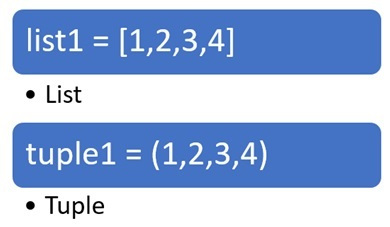
\includegraphics[width=0.5\textwidth]{figures/Difference-Between-List-and-Tuple-fig-1-2.jpg}
\caption{At first glance list and tuples look very similar, but they are not\ldots}
\label{fig:tuples}
\end{figure}

Like lists, tuples are containers of any type of object. Unlike lists though they are \emph{immutable} which means that once they have been created the content cannot be changed (i.e. no append, insert or delete of the elements). Furthermore since they are immutable they can be used as dictionary keys (lists cannot). To create a tuple the comma-separated list of items has to be enclosed in brackets, or the \texttt{tuple()} operator can be used. Accessing tuple items is done in exactly the same way as lists.

\begin{ipython}
atuple = (1, 2, 3)
print (f"Length: {len(atuple)}")
print (f"First element: {atuple[0]}")
print (f"Last element: {atuple[-1]}")
\end{ipython}
\begin{ioutput}
Length: 3
First element: 1
Last element: 3
\end{ioutput}

In the next snippet of code it is shown the so called unpacking which is another way to assign tuple values to variables.

\begin{ipython}
x, y, z = (10, 5, 12)
print (f"coord: x={x} y={y} z={z}")
\end{ipython}
\begin{ioutput}
coord: x=10 y=5 z=12
\end{ioutput}

If a tuple has just one element don't forget the comma at the end otherwise it will be treated as a single number.

\begin{ipython}
tuple2 = (1,)
print(type(tuple2))

tuple2 = (1)
print(type(tuple2))
\end{ipython}
\begin{ioutput}
<class 'tuple'>
<class 'int'>
\end{ioutput}

Since a tuple is immutable to add new elements it is necessary to create a new object:

\begin{ipython}
tuple1 = (1, 2, 3)
tuple2 = tuple1 + (4, 5)
print(tuple2)
\end{ipython}
\begin{ioutput}
(1,2,3,4,5)
\end{ioutput}

As already said tuples can be used as dictionary keys:

\begin{ipython}
d = {
	('Finance', 1): 'Room 8',
	('Finance', 2): 'Room 3',
	('Math', 1): 'Room 6',
	('Programming', 1): 'IT room'}
\end{ipython}

Below the full list of tuple functions:
\begin{ipython}
dir(dict)
\end{ipython}
\begin{ioutput}
[...
 'count',
 'index']
\end{ioutput}

\section*{Exercises}
\begin{question}
What is a dictionary in \(\tt{python}\) programming language ? Create a dictionary, modify it and then print all its items.
\end{question}

\cprotEnv\begin{solution}
A dictionary is a container that maps a key (any object) to a value (any object), contrary to lists which map an integer (the index) to a value (any object).

\begin{ipython}
dictionary = {"calculus": 28, "physics":30, "chemistry":25}

dictionary["laboratory"] = 27
dictionary["chemistry"] = 24

print ("Exam\tVote")
for k, v in dictionary.items():
    print("{}:\t{}".format(k, v))
\end{ipython}
\begin{ioutput}
Exam            Vote
calculus:       28
physics:        30
chemistry:      24
laboratory:     27
\end{ioutput}
\end{solution}

\begin{question}
Write code which, given the following list 

\lstinline[language=iPython]|input\_list = [3, 5, 2, 1, 13, 5, 5, 1, 3, 4]|

\noindent
prints out the indices of every occurrence of \lstinline[language=iPython]|y=5|.
\end{question}

\cprotEnv\begin{solution}
\begin{ipython}
l = [3, 5, 2, 1, 13, 5, 5, 1, 3, 4]

for i in range(len(l)):
    if l[i] == y:
        print (i)
\end{ipython}
\begin{ioutput}
1
5
6
\end{ioutput}
Note that lists already have a way to get the occurrences of an item: \texttt{l.count(5)} would have done the job.
\end{solution}

\begin{question}
Write a \texttt{python} program to convert a list of tuples into a dictionary where the keys are the first elements of each tuples and the values the second.

\noindent
Input: \lstinline[language=iPython]|l = [("x", 1), ("x", 2), ("x", 3), ("y", 1), ("y", 2), ("z", 1)]|
\end{question}

\cprotEnv\begin{solution}
\begin{ipython}
l = [("x", 1), ("x", 2), ("x", 3), ("y", 1), ("y", 2), ("z", 1)]

d = {}
for item in l:
    d[item][0]] = item[1]
    
print(d)
\end{ipython}
\begin{ioutput}
{'x': 3, 'y': 2, 'z': 1}
\end{ioutput}
Note that there is just one occurrence of the key $\tt{x}$ and $\tt{y}$ because keys has to be unique and setting the same key to a different value simply overwrite the existing entry.
\end{solution}

\begin{question}
Write a \texttt{python} program to increment by 10 the last value of each tuples in a list.

\noindent
Input: \lstinline[language=iPython]|l = [(10, 20, 40), (40, 50, 60), (70, 80, 90)]|.
\end{question}

\cprotEnv\begin{solution}
\begin{ipython}
l = [(10, 20, 40), (40, 50, 60), (70, 80, 90)]

for i in range(len(l)):
    new_tuple = l[:-1] + [l[2] + 10]
    l[i] = new_tuple
    
print (l)
\end{ipython}
\begin{ioutput}
[(10, 20, 50), (40, 50, 70), (70, 80, 100)]
\end{ioutput}
\end{solution}

\begin{question}
Write a \texttt{python} program to count the elements in a list until an element is a tuple.

\noindent
Input:\lstinline[language=iPython]|l = [1, 5, 'a', (1, 2), 'test':1]|
\end{question}

\cprotEnv\begin{solution}
\begin{ipython}
l = [1, 5, 'a', (1, 2), 'test':1]

number_of_items = 0 
for item in l:
    if type(item) != 'tuple'{:}
        number_of_items += 1
    else:
        break
        
print("There are {} items before a tuple.".format(number_of_items))
\end{ipython}
\begin{ioutput}
\end{ioutput}
\end{solution}

\begin{question}
Write a \texttt{python} script to concatenate the following dictionaries to create a new single one.

\noindent 
Input:
\lstinline[language=iPython]|dic1 = \{1:10, 2:20\}; dic2 = \{3:30, 4:40\}; dic3 = \{5:50, 6:60\}|
\end{question}

\cprotEnv\begin{solution}
\begin{ipython}
dic1 = {1:10, 2:20}
dic2 = {3:30, 4:40}
dic3 = {5:50, 6:60}

dic_tot = dict()
dic_tot.update(dic1)
dic_tot.update(dic2)
dic_tot.update(dic3)

print(dic_tot)
\end{ipython}
\begin{ioutput}
{1: 10, 2: 20, 3: 30, 4: 40, 5: 50, 6: 60}
\end{ioutput}

An alternative and even more concise way using the \texttt{**} operator is the following:
\begin{ipython}
dic1 = {1:10, 2:20}
dic2 = {3:30, 4:40}
dic3 = {5:50, 6:60}

new_dic = {**dic1, **dic2, **dic3}
\end{ipython}
\end{solution}

\begin{question}
Write a \texttt{python} script to check whether a given key already exists in a dictionary.
\end{question}

\cprotEnv\begin{solution}
\begin{ipython}
dic = {"a":1, "b":2, "c":3}

print("z" in dic)
print("a" in dic)
\end{ipython}
\begin{ioutput}
False
True
\end{ioutput}
\end{solution}

\begin{question}
Write a \texttt{python} program to combine two dictionary adding values for common keys.

\noindent
Input: \lstinline[language=iPython]|d1 = \{'a':100, 'b':200, 'c':300\}; d2 = \{'a':300, 'b':200, 'd':400\}|
\end{question}

\cprotEnv\begin{solution}
\begin{ipython}
d1 = {'a':100, 'b':200, 'c':300}
d2 = {'a':300, 'b':200, 'd':400}

d = {}
d.update(d1)

for k in d2.keys():
    if k in d:
        d[k] = d[k] + d2[k]
    else:
        d[k] = d2[k]

print(d)
\end{ipython}
\begin{ioutput}
{'a': 400, 'b': 400, 'c': 300, 'd': 400}
\end{ioutput}
\end{solution}

\begin{question}
Given the following dictionary mapping currencies to 2-year zero coupon bond prices, build another dictionary mapping the same currencies to the corresponding annualized interest rates.

\lstinline[language=iPython]|d = {'EUR':0.9, 'CHF':1.005, 'USD':0.985, 'GBP':0.97}|
\end{question}

\cprotEnv\begin{solution}
The price of a n-years zero coupon bond is:

\[ P = \frac{M}{(1+r)^{n}} = M\cdot D \]
where $M$ is the value of the bond at the maturity, $r$ is the risk-free rate and $n$ is the number of years until maturity.
%Hence:

\[ D = \cfrac{1}{(1+r)^{n}} \implies r = \Big(\cfrac{1}{D}\Big)^{\cfrac{1}{n}} - 1\]

\begin{ipython}
# initialize an empty dictionary in which to store result
rates = {}

maturity = 2
discount_factors = {'EUR':0.9, 'CHF':1.005, 'USD':0.985, 'GBP':0.97}

# loop over the input dictionary to get the currencies
for currency, df in discount_factors.items():
    # calculate the rate and store it in the output dictionary
    rates[currency] = pow(1/df, 1/maturity) - 1
   
for r in rates.items():
    print(r)
\end{ipython}
\begin{ioutput}
('EUR', 0.05409255338945984)
('CHF', -0.002490663892367073)
('USD', 0.007585443719756668)
('GBP', 0.015346165133619083)
\end{ioutput}
\end{solution}

\begin{thebibliography}{9}
\bibitem{lists} \href{https://docs.python.org/3/tutorial/datastructures.html}{\emph{Data Structures, More on Lists}} [Online]
\bibitem{dictionaries} \href{https://realpython.com/python-dicts/}{\emph{Dictionaries in Python}}, Real Python [Online]
\bibitem{tuple} \href{https://www.programmareinpython.it/video-corso-python-base/14-liste-e-tuple/}{\emph{Liste e Tuple}}, Programmare in Python [Online]
\end{thebibliography}

 % da riguardare
\chapter{Object Oriented Programming with \texttt{python}}
\label{ch:oop}

In this Chapter the main characteristics that makes \texttt{python} an \textit{object oriented programming} (OOP) language will be reviewed. Before however the concepts of function and variable scope will be outlined.

\section{Functions}
\label{functions}

A function is a block of organized, reusable code that is used to perform a single action. Functions provide better modularity for your application and high degree of code reusing. To define a function the keyword \texttt{def} is used, followed by the name of the function and by the required parameters in parenthesis. Functions are called by name passing the necessary parameters, if any.

\begin{ipython}
# sum up all the integers between 1 and n
def my_function(n): # this function take one input only (n)
    x = 0
    for i in range(1, n+1):
        x += i
    return x # the function returns a number

my_function(5) # 5 + 4 + 3 + 2 + 1
\end{ipython}

Functions can return any kind of objects (numbers, strings, lists, complex objects\ldots) but it is not mandatory to have a return value, so you can have functions \textbf{without} a \texttt{return} statement (e.g. a function that simply take a string as input and print it to screen with a particular format).
In addition the syntax of the \texttt{return} is different from other languages like \texttt{Visual\ Basic}; the returned object doesn't have to have the same name as the function. Indeed above the variable \texttt{x} is returned and not the variable \texttt{my\_function}. Below an example of function not returning.

\begin{ipython}
def printing(mystring):
    print ((myString).upper())
\end{ipython}

Functions can call other functions (once a function has been defined it can be accessed from everywhere within the same file or notebook): here \texttt{my\_function\_2} calls \texttt{my\_function}

\begin{ipython}
def my_function_2(n, x):
    return f"The result is : {my_function(n)*x}")

my_function_2(5, 10)
\end{ipython}

Functions can also call themselves too (i.e \emph{recursion}). In the next example we see a function that computes the factorial exploiting the following Eq.~\ref{eq:factorial}

\begin{equation}
\begin{cases}
    n! = n \times (n-1)! & \;\; (\forall n > 1) \\
    n! = 1 & \;\; (\forall n \le 1)
\end{cases}
\label{eq:factorial}
\end{equation}

\begin{ipython}
def factorial(n):
    if n <= 1:
        return 1
    else:
        return n * factorial(n-1)

factorial(10)
\end{ipython}

In this example the function \texttt{factorial} is initially called with the input corresponding to the factorial we want to compute, it then calls itself each time with the argument \texttt{n-1}, multiplying together all the results. The previous example is quite simple but recursion can be tricky sometimes so apply it with caution. 

Function input parameters can have default values, which means that a function that works with some input values can be called with less parameters provided their default values have been specified.

In the following example the function \texttt{powers} takes three inputs: a list of numbers, an exponent (\texttt{n}) and a constant (\texttt{c}). The code loops through the provided list of numbers and process them according to the formula 

\begin{equation*}
item^{n} + c
\end{equation*}
finally it puts the results in a new list which will be finally returned.

\begin{ipython}
def powers(l, n=2, c=0):
    return [item**n+c for item in l]

print (powers([5, 11, 6], 3, 4))
print (powers([5, 11, 6]))
\end{ipython}
\begin{ioutput}
[129, 1335, 220]
[25, 121, 36]
\end{ioutput}
    
As you can see the function is called twice with two different set of parameters: in the first case we pass the list of numbers, the exponent and the constant, in the second just the same list of numbers.
In the latter case, being defined the default values for \texttt{n} and \texttt{c}, the function works perfectly well, fewer inputs are provided and the missing ones are replaced by their defaults. 

When calling a function, parameters can be passed also by name for clarity, in this case of course the order doesn't matter. Compare the two results below:

\begin{ipython}
def func(a, b, c):
    return a + b * c

print (func(c=4, b=2, a=1))
print (func(4, 2, 1))
\end{ipython}
\begin{ioutput}
9
6
\end{ioutput}

In the first case the function is called by name, in the second case the parameter are implicitly assigned according to their position.

\subsubsection{\texttt{args} and \texttt{kwargs}}
\label{sec:kwargs_args}

Another possible way of passing parameters to a function is through the reserved words \texttt{args} and \texttt{kwargs}. Those are very useful especially if there are nested call to function (a function that call another function) and we need to specify parameters for the  secondary call. Let's see first a usage example of \texttt{args}.

Imagine you have to call a function \texttt{runner} which multiplies by two the result returned by another function, \texttt{func}, which takes in inputs three parameters \texttt{a, b, c}. A first option is too define \texttt{a, b, c} in the \emph{global scope} (see Section~\ref{sec:var_scope}) so that the three of them are visible within \texttt{func}.
\begin{ipython}
a = 10
b = 1
c = 5

def func(x):
    return a*x**2 + b*x + c

def runner(f, x):
    return f(x)*2

print (runner(func, 2))
\end{ipython}
\begin{ioutput} 	
94
\end{ioutput}

This is not ideal though. If I had to run multiple times the calculation changing every time one of the three parameters I would be in troubles. The solution is to use \texttt{args} and the \texttt{*} operator. Indeed I can assign a tuple or list to \texttt{args}, where each item corresponds to one of the parameters to pass to \texttt{func} and then, inside \texttt{runner} we can call \texttt{func} with \texttt{*args} as second parameter. This will expand the tuple (or list) associated to \texttt{args} assigning each item to the corresponding parameter in the function call.

\begin{ipython}
def func2(x, a, b, c):
    return a*x**2 + b*x + c

def runner(f, x, args=()):
    return f(x, *args)*2

print (runner(func2, 2, args=(10, 1, 5)))
\end{ipython}
\begin{ioutput} 	 
94
\end{ioutput}

\texttt{kwargs} acts similarly to \texttt{args} except that now the parameter are passed by name. It is indeed a dictionary and each key should correspond to a function parameter name. The call now will have two asterisks (\texttt{**}) to expand the dictionary.
 
\begin{ipython}
def func2(x, a, b, c):
    return a*x**2 + b*x + c

def runner(f, x, kwargs={}):
    return f(x, **kwargs)*2

print (runner(func2, 2, kwargs={"a":10, "b":1, "c":5}))
\end{ipython}
\begin{ioutput} 	  
94
\end{ioutput}
  
The last feature to describe is that we can associate an help message to functions so that we can easily check what they are for by simply asking \texttt{help(functioName)}:

\begin{ipython}
def powers(l, n=2, c=0):
    """
    a shifted power function example
    """
    return [item**n+c for item in l]

help(powers)
\end{ipython}
\begin{ioutput} 	  
Help on function powers in module __main__:

powers(l, n=2, c=0)
    a shifted power function example
\end{ioutput}

\textbf{Remember, it is always very important to document your code !} Doing so also keep in mind that \emph{commenting} is not the same as \emph{documenting}. Code itself tells you \textbf{how}, comments tell you \textbf{why}, and documentation describes its use and functionality to the users.

Sometimes, you come to realize that the documentation is lacking or even worse, missing entirely. This is a frustrating feeling that deters you from using a library, no matter how great or efficient the code is.
Let me quote a couple of statements done by \texttt{python} experts:
\begin{quote}
“Code is more often read than written.”\\
\null\hfill— Guido van Rossum
\\\\
“It doesn’t matter how good your software is, because if the documentation is not good enough, people will not use it.“\\
\null\hfill— Daniele Procida
\end{quote}

\section{Variable Scope}
\label{sec:var_scope}

Not all variables are accessible from all parts of our program, and not all variables exist for the entire lifetime of the program. The part of a program where a variable is accessible is called its \emph{scope}.

A variable which is defined in the main body, sometimes referred to as global namespace i.e. the code block which is not indented at all of a script, is called a \emph{global variable}. It will be visible throughout the file, and also inside any file which imports that file. Global variables can have unintended consequences because of their wide-ranging effects, that is why you should almost never use them and they are usually represented by an uppercase name. Only objects which are intended to be used really globally, like functions and classes (which will be introduced in the next Section~\ref{sec:class}), should be put in the global namespace.

Global variables cannot be accessed directly inside functions but before using them they have to be named in a special statement starting with the keyword \texttt{global}. Essentially \texttt{global} tells \texttt{python} that in the following function we want to use the listed global variable.
Imagine a global variable \texttt{AGLOBALPARAM} has been defined at the beginning of a program, 
in the example below few cases are outlined:
\begin {itemize}
\tightlist
\item a function that read the value of \texttt{AGLOBALPARAM} without modifying it;
\item a function that read and modify \texttt{AGLOBALPARAM};
\item and a function that throws an exception (i.e. an error in technical language) because it has been badly coded.
\end{itemize}

\begin{ipython}
AGLOBALPARAM = 10

# Here you just use AGLOBALPARAM value, but do not modify it
# param is just a local copy of AGLOBALPARAM
def multiplyParam(param):
    param = param * 10
    return (param)

# Here you actually use AGLOBALPARAM
# you modify it directly with the global command
def divideParam():
    global AGLOBALPARAM
    AGLOBALPARAM = AGLOBALPARAM / 10
    return (AGLOBALPARAM)

# Here you try to use AGLOBALPARAM but gives you an error
# AGLOBALPARAM is not defined in the function body
# and the global command has not been used neither
def sumParam():
    AGLOBALPARAM = AGLOBALPARAM + 10
    return (AGLOBALPARAM + x)

print (f"AGLOBALPARAM is {AGLOBALPARAM} to start.")
print ("Let's multiply it by 10.")
multiplyParam(AGLOBALPARAM)

print (f"AGLOBALPARAM is still {AGLOBALPARAM}")
print ("Let's divide it by 10")
divideParam()

print (f"Now AGLOBALPARAM is {AGLOBALPARAM}")
print ("Let's sum it to 10")
sumParam()
\end{ipython}

A variable which is defined in a block of code is said to be local to that block. Examples of local scopes are: functions, \texttt{for} or \texttt{while} loops, \texttt{if} blocks\ldots In case of a function it means that a local variable will be accessible from the point at which it is defined until the end of the function itself (e.g. function parameters are examples of local variables).

\begin{ipython}
# functions are not evaluated until their are not called
def test_scope(max_val):
    for i in range(max_val):
        print (i)
    print (f"max_val in 'test_scope' function is {max_val}")

# the Python interpreter starts evaluating the code from here
max_val = 10
test_scope(5)
print (f"max_val in global scope is {max_val}")
print (i)
\end{ipython}

In the previous example we have defined two \texttt{max\_val} variables, one which is global and it has been initially set to 10, another one which is local to the \texttt{test\_scope} function.
Try as much as possible to choose different names for each variable you are going to use in a program to avoid confusions and mistakes which may lead to unexpected behavior of your code.

As a last example compare the following \texttt{for} loops: the first one, correctly written, loops with the variables \texttt{i} and \texttt{j}, in the second one \texttt{j} has been replaced by \texttt{i}, note how this is perfectly legal but the result changes dramatically:

\begin{ipython}
a = [["a", "b", "c"],["d", "e", "f"],["g", "h", "i"]]

for i in range(3):
    for j in range(3):
        print (a[i][j])
\end{ipython}
\begin{ioutput} 	  
a
b
c
d
e
f
g
h
i
\end{ioutput}

\begin{ipython}
a = [["a", "b", "c"],["d", "e", "f"],["g", "h", "i"]]

for i in range(3):
    for i in range(3):
        print (a[i][i])
\end{ipython}
\begin{ioutput} 	  
a
e
i
a
e
i
a
e
i
\end{ioutput}

\section{Classes}
\label{sec:class}

Classes are a key ingredient of \emph{Object Oriented Programming} and their concept is implemented basically in every modern programming language like \texttt{python}, \texttt{Java} and \texttt{C++}. OOP is a programming model in which programs are organized around data, or objects, rather than functions and logic.
\textbf{Any object can be thought of as a dataset with unique attributes and behavior} (examples can range from physical entities, such as a human being that is described by properties like name and birthday, to abstract concepts as a discount curve). This opposes the historical 
approach to programming where emphasis was placed on how the logic was written rather than how to define data within the logic. In this framework classes are a mean for creating objects (a particular data structure), providing initial values for its state (member variables or attributes), and implementations of behavior (member functions or methods).
Let's summarize here some terminology:

\vspace*{.5cm}
\begin{tabular}{rl}
  CLASS $\rightarrow$ & collection of functions that operate on some dataset \\
  DATA ITEMS $\rightarrow$ & the \textbf{attributes} of the class \\
  CLASS INSTANCE $\rightarrow$ & \noindent\begin{tabular}{@{}l}a specific collection of data belonging to the particular \\object we are representing\end{tabular}\\
  CLASS FUNCTIONS $\rightarrow$ & \textbf{methods} of the class, act on class \textbf{instances} \\
\end{tabular}
\vspace*{.5cm}

\textbf{In other words classes are collections of functions that operate on a dataset, and instances of that class represent individual datasets (or if you prefer a specialization of that class).}

Class examples are: a building (with number of entrances, number of floors, a flag to know if there is a garden\ldots), a dog (with age, fur color\ldots) or a computer (with manufacturer, RAM size, CPU type\ldots).
While examples of corresponding instances are: the Empire State Building (a specific building), Lassie (a very particular dog), or your computer, see Fig.~\ref{fig:classes}.

\begin{figure}[htb]
  \centering
  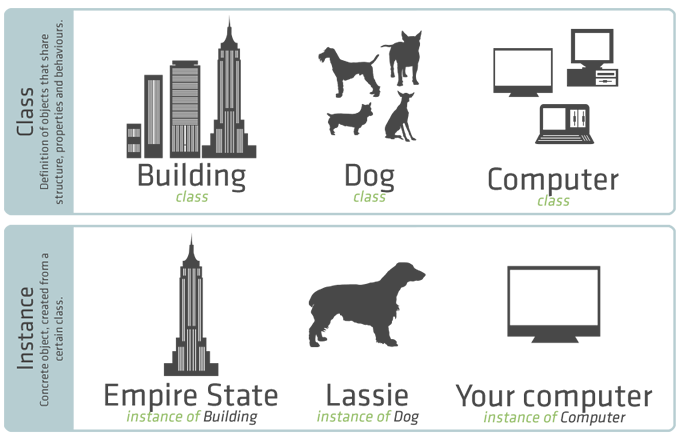
\includegraphics[width=0.8\linewidth]{figures/classes_instances.png}
  \caption{Graphical representation of a class instance.}
  \label{fig:classes}
\end{figure}

To see how classes can be defined let's try to code one representing a person:
\begin{ipython}
from datetime import date        

class Person:
\end{ipython}

First of all, if needed, we have to import the necessary modules, in this case the \texttt{datetime} module is used to manage the person age.
Then the \texttt{class} keyword followed by the class name is used to start the actual definition.

\subsubsection{The Constructor Method}\label{the-constructor-method}

After declaring the class name, the constructor method must be defined. In \texttt{python}, this is denoted by \texttt{\_\_init\_\_()} regardless the class name. The \texttt{\_\_init\_\_} method, as every other method in a class, takes \texttt{self} as the first argument, and then any number of parameters as desired by the programmer. The \emph{constructor} allows to specify the initial state of a class by setting its attribute values. For this example that describes a person, the programmer wants to know its name, the birthday and a job (this last one won't be initialize by the constructor though).

The \texttt{self} parameter is used to create class attributes. Variables whose name starts with \texttt{self.} have \emph{class scope}, which means are available within each class method. To use the parameters and associate them with a particular instance of the class, within the \texttt{\_\_init\_\_} method, create variables for each argument like this: \texttt{self.variableName\ =\ param}.

\begin{ipython}
from datetime import date

# this is the class definition
# usually classes use camel naming convention
class Person:
    # the special method __init__ allows to instantiate a class
    # with an initial dataset
    def __init__(self, name, birthday):
        self.name = name
        self.birthday = birthday
        self.occupation = None # this attribute not set at instantiation
\end{ipython}

Now that we have a class definition that represents a generic person we can specialized it to some real person.

\begin{ipython}
me = Person("Matteo", date(1974, 10, 20))
print (type(me))
\end{ipython}
\begin{ioutput}
<class '\_\_main\_\_.Person'>
\end{ioutput}

When we instantiate a class, \texttt{python} first calls the \texttt{\_\_init\_\_} method and initializes the attributes with the parameter we are passing.

\subsubsection{Class Methods}

We haven't yet defined any "person behavior", so let's add a couple of methods to our class: one computing the person's age and the other setting its primary occupation.

\begin{ipython}
class Person:
    def __init__(self, name, birthday):
        self.name = name
        self.birthday = birthday
        self.employment = None

    # this is a normal method and will work on some class attribute
    def age(self, d=date.today()):
        age = (d - self.birthday).days/365
        print (f"{self.name} is {age:.0f} years old")

    def mainOccupation(self, occupation):
        self.employment = occupation
        print (f"{self.name}'s main occupation is: {self.employment}")
\end{ipython}

To access class attributes and methods the dot (\texttt{.}) operator has to be used. 

\begin{ipython}
print (me.name)
\end{ipython}
\begin{ioutput}
'Matteo'
\end{ioutput}
        
\begin{ipython}
me.age(date.today())
\end{ipython}
\begin{ioutput}
Matteo is 46 years old
\end{ioutput}

\subsection{Inheritance and Overriding Methods}
\label{inheritance-and-overriding-methods}

Inheritance is basically the idea that different classes can have similar components, and in order to avoid repeating code, it is used to link parent to descendant classes. Inheritance allows the classes to share information relevant to multiple parts of the code.

For example, in a fantasy story, there are \emph{heroes} and \emph{monsters} but both of them are \emph{characters}. Similarly \emph{dragons} and \emph{orcs} are \emph{monsters}. Though they are different kind of monsters, they share some characteristics: they both have a color, a size and enemies. Orcs might have characteristics that dragons do not; for example which kind of weapon the orc carries (Fig.~\ref{fig:inheritance}). 

\begin{figure}[h]
  \centering
  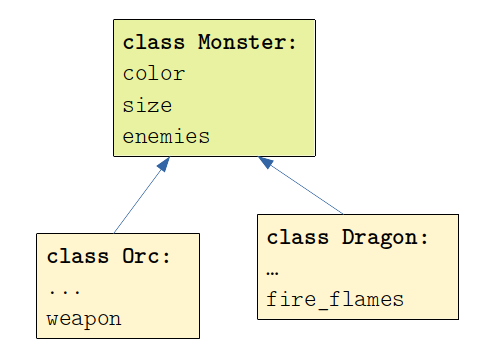
\includegraphics[width=0.5\textwidth]{figures/inheritance.png}
  \caption{Example of inheritance: both \texttt{Dragon} and \texttt{Orc} inherits from \texttt{Monster}, but both add additional attributes that qualify better each "monster features".}
  \label{fig:inheritance}
\end{figure}

Inheritance allows code to be reused and reduces the complexity of a program. The derived classes (descendants) override or extend the functionalities of the base classes (ancestors). To see how it works in more detail two derived class will be implemented from \texttt{Person}: \texttt{Adult} and \texttt{Child}.

\begin{ipython}
class Adult(Person):
    def __init__(self, name, birthday, drv_license_id):
        Person.__init__(self, name, birthday) # this is a special syntax
        self.drv_license_id = drv_license_id

class Child(Person):
    def mainOccupation(self):
        self.employment = "schoolchild"
        print (f"{self.name} is a {self.employment}")
\end{ipython}

Inheritance is specified in parenthesis after the class name. \texttt{Child} still inherits from \texttt{Person} and modifies it by setting the only occupation allowed for a child, overriding the \texttt{mainOccupation} method. \texttt{Adult} class inherits from \texttt{Person} too but extends it adding a new attribute, i.e. the driving license id. 

\begin{ipython}
pippo = Adult("Goofy", date(1936, 1, 1), "A1234")
qui = Child("Huey", date(2014, 10, 9))
\end{ipython}

Behind the scenes, when instantiating a \texttt{Child} class, the constructor of \texttt{Person} is called and the attributes, \texttt{name} and \texttt{birthday} are still initialized.  

For the \texttt{Adult} class things are a little bit different because a new attribute has been added, so we need to code its own constructor where we first call explicitly the \texttt{Person}'s constructor (\texttt{Person.\_\_init\_\_(self, \ldots)} and then we initialize the new attribute.

\begin{ipython}
pippo.age()
pippo.mainOccupation("Comic's character")
\end{ipython}
\begin{ioutput}
Goofy is 85 years old
Goofy's main occupation is: Comic's character
\end{ioutput}

\begin{ipython}
qui.age()
qui.mainOccupation()
\end{ipython}
\begin{ioutput}
Huey is 6 years old
Huey is a schoolchild
\end{ioutput}

\section*{Exercises}
\cprotEnv\begin{question}
Calculate the prices of calls with various strikes, using the following input data.

\begin{ipython}
s = 800 
# strikes expressed as percentage of spot price
moneyness = [0.5, 0.75, 0.825, 1.0, 1.125, 1.25, 1.5]
vol = 0.3
ttm = 0.75
r = 0.005
\end{ipython}
\noindent
The output should be a dictionary mapping strikes to call prices.
\end{question}

\cprotEnv\begin{solution}
\begin{ipython}
import numpy as np
from scipy.stats import norm

def d1(S, K, r, vol, ttm):
    num = np.log(S/K) + (r + 0.5*np.power(vol, 2)) * ttm
    den = vol * np.sqrt(ttm)
    return num/den

def d2(S, K, r, vol, ttm):
    return d1(S, K, r, vol, ttm) - vol*np.sqrt(ttm)

def call(S, K, r, vol, ttm):
    return (S * norm.cdf(d1(S, K, r, vol, ttm)) - \
           K*np.exp(-r*ttm)*norm.cdf(d2(S, K, r, vol, ttm)))

S = 800
# strikes expressed as % of spot price
moneyness = [0.5, 0.75, 0.825, 1.0, 1.125, 1.25, 1.5]
vol = 0.3
ttm = 0.75
r = 0.005

result = {}
for m in moneyness:
    result[S*m] = round(call(S, S*m, r, vol, ttm), 2)
print(result)
\end{ipython}
\begin{ioutput}
{400.0: 401.66, 
 600.0: 213.99, 
 660.0: 166.86, 
 800.0: 84.04, 
 900.0: 47.62, 
 1000.0: 25.63, 
 1200.0: 6.66}
\end{ioutput}
\end{solution}

\cprotEnv\begin{question}
Write two classes, \texttt{Circle} and \texttt{Rectangle} that given the radius and height, width respectively allow to compute area and perimeter of the two shapes. Test them with the following:

\begin{ipython}
a_circle = Circle(5)
print(f"My circle has an area of {a_circle.area()} m2")

a_rectangle = Rectangle(3, 6)
print (f"My rectangle has a perimeter of {a_rectangle.perimeter()} m and an area of {a_rectangle.area()} m2")
\end{ipython}
\end{question}

\cprotEnv\begin{solution}
\begin{ipython}
from math import pi

class Circle:
    def __init__(self, radius):
        self.radius = radius

    def area(self):
        return pi*self.radius**2

class Rectangle:
    def __init__(self, width, height):
        self.height = height
        self.width = width

    def area(self):
        return self.width*self.height

    def perimeter(self):
        return self.width*2 + self.height*2

circle = Circle(5)
print (f"My circle area is {circle.area():.1f} m**2")

rect = Rectangle(3, 6)
print (f"My rect area is {rect.area():.1f} m**2 and the perimeter is {rect.perimeter()} m")
\end{ipython}
\begin{ioutput}
My circle area is 78.5 m**2
My rect area is 18.0 m**2 and the perimeter is 18 m
\end{ioutput}
\end{solution}

\cprotEnv\begin{question}
Write a class \texttt{Menu} which is a component of a restaurant ordering system. Through this program the waiters should be able to: register client orders adding or deleting dishes and print the final bill.
The only attribute of the class is the following list of dishes with an \texttt{id} to identify them, their name and cost.

\begin{ipython}
dishes = {'1':("Spaghetti", 6.50), '2':("Pizza", 7.00), '3':("Water", 0.50),
                       '4':("Red Wine 0.5l", 5.00)}
\end{ipython}
\noindent
To test the class simulate an order and print the corresponding bill.
\end{question}

\cprotEnv\begin{solution}
\begin{ipython}
class Menu:
    def __init__(self):
        self.dishes = {'1':("Spaghetti", 6.50), '2':("Pizza", 7.00), '3':("Water", 0.50),
                       '4':("Red Wine 0.5l", 5.00)}
        self.current_choice = {}
        
    def clear_order(self):
        self.current_choice = {}
        
    def add_dish(self, dish_id, quantity = 1):
        if dish_id not in self.dishes.keys():
            print (f"Dish {dish_id} currently not available.")
        else:
            self.current_choice[dish_id] = 
                self.current_choice.setdefault(dish_id, 0) + quantity
            
    def remove_dish(self, dish_id, quantity = 1):
        if dish_id in self.current_choice.keys():
            self.current_choice[dish_id] = max(0, self.current_choice[dish_id] - quantity)
            
    def bill(self):
        cost = 0
        for id, qty in self.current_choice.items():
            cost += self.dishes[id][1] * qty
            print (f"{self.dishes[id][0]:15} {qty:2} {self.dishes[id][1]:>6.2f}")
        print ("{'Tot:':15}    {cost:>6.2f}")

m = Menu()
m.add_dish('1')
m.add_dish('2')
m.add_dish('3')
m.bill()
\end{ipython}
\begin{ioutput}
Spaghetti        1   6.50
Pizza            1   7.00
Water            1   0.50
Tot:                14.00
\end{ioutput}
\end{solution}

\begin{question}
Define a Point2D class that represent a point in a plane. Its \texttt{\_\_init\_\_} method should accept the point coordinates \texttt{x} and \texttt{y}. Write a method \texttt{distanceTo} that compute the distance of the point to another passed as input. Test the class by printing the distance of the point $P=(4, 5)$ to the origin $P=(0,0)$ and to $P=(3,4)$.

\noindent\textbf{Hint:} in the Cartesian plane the distance between two points is: $\sqrt{(x_1 - x_2)^2 + (y_1 - y_2)^2}$.
\end{question}

\cprotEnv\begin{solution}
\begin{ipython}
from math import sqrt

class Point2D:
    def __init__(self, x, y):
        self.x = x
        self.y = y

    def distanceTo(self, x, y):
        dist = sqrt((self.x-x)**2 + (self.y - y)**2)
        return dist

    def distanceTo_v2(self, p):
        dist = sqrt((self.x-p[0])**2 + (self.y - p[1])**2)
        return dist

    def distanceTo_v3(self, p):
        dist = sqrt((self.x-p.x)**2 + (self.y - p.y)**2)
        return dist

point = Point2D(4, 5)
p0 = (0, 0)
point0 = Point2D(0, 0)
print (f"distance to p0: {point.distanceTo(p0[0], p0[1]):.2f}")
print (f"distance_v2 to p0: {point.distanceTo_v2(p0):.2f}")
print (f"distance_v3 to p0: {point.distanceTo_v3(point0):.2f}")
\end{ipython}
\begin{ioutput}
distance to p0: 6.40
distance_v2 to p0: 6.40
distance_v3 to p0: 6.40
\end{ioutput}
\begin{ipython}
p1 = (3, 4)
point1 = Point2D(3, 4)
print (f"distance to p1: {point.distanceTo(p1[0], p1[1]):.2f}")
print (f"distance v2 to p1: {point.distanceTo_v2(p1):.2f}")
print (f"distance v3 to p1: {point.distanceTo_v3(point1):.2f}")
\end{ipython}
\begin{ioutput}
distance to p1: 1.41
distance v2 to p1: 1.41
distance v3 to p1: 1.41
\end{ioutput}
\end{solution}

\cprotEnv\begin{question}
Write a class \texttt{Student} which inherits from the class \texttt{Person} defined in Chapter Object Oriented Programming in Python. This new class should have two new attributes: \texttt{grade} which keeps the type of school and \texttt{votes} a dictionary which will record the student's votes and the corresponding course. Then add two methods, one to add votes and another to compute the average vote.Instantiate a "student" add some votes and show how good it has been.

\noindent\textbf{Hint:} this is the \texttt{Person} class already developed.

\begin{ipython}
class Person:
    def __init__(self, name, birthday):
        self.name = name
        self.birthday = birthday
        self.employment = None

    def age(self, d=date.today()):
        age = (d - self.birthday).days/365
        print (f"{self.name} is {age:.0f} years old")

    def mainOccupation(self, occupation):
        self.employment = occupation
        print ("{self.name}'s main occupation is: {self.employment}")
\end{ipython}
\end{question}

\cprotEnv\begin{solution}
\begin{ipython}
class Student(Person):
    def __init__(self, name, birthday, school):
        Person.__init__(self, name, birthday)
        self.grade = school
        self.votes = {}

    def addVote(self, subject, vote):
        self.votes[subject] = vote

    def average(self):
        print ("List of votes")
        print ("-------------")
        for k, v in self.votes.items():
            print (f"{k}: {v}")
        avg = sum(self.votes.values())/len(self.votes)
        print ("-------------")
        print (f"Avg: {avg:.1f}")

student = Student("Mario", date(1980, 5, 6), "Liceo Scientifico G. Galilei")
student.addVote("Calculus", 8)
student.addVote("Literature", 5.5)
student.addVote("Latin", 6.5)
student.average()
\end{ipython}
\begin{ioutput}
List of votes
-------------
Calculus: 8
Literature: 5.5
Latin: 6.5
-------------
Avg: 6.7
\end{ioutput}
\end{solution}

 % da riguardare
\chapter{Date and Time}
\label{sec:datetime}

In this Chapter we take a little break and concentrate on a topic that it is not usually covered in a \texttt{python} review for beginners. However given its importance for financial computation the next paragraphs will be devoted to a close look up on the \texttt{datetime} module~\cite{bib:datetime}, whose usage will help in manipulating dates.

\section{Dates}\label{dates}

As said dates are not usually included in a standard \texttt{python} tutorial, however since they
are pretty essential for finance we are going to cover this topic in some detail.
In \texttt{python} the date utilities mainly lives in the \texttt{datetime} module. Briefly we are
also going to show \texttt{relativedelta} from the \texttt{dateutil} module, which allows to
add/subtract days/months/years to dates, in other words to make operations on them.

In this first example today's date is defined and with \texttt{relativedelta} two more dates are created
adding two months and subtracting three days to the first one.

\begin{ipythonnon}
from datetime import date, datetime
from dateutil.relativedelta import relativedelta

date1 = date.today()
print(date1)

date2 = date.today() + relativedelta(months=2)
print(date2)

date3 = date.today() - relativedelta(days=3)
print(date3)
\end{ipythonnon}
\begin{ioutput}
2020-08-03
2020-10-03
2020-07-31
\end{ioutput}

There is another way of computing a new date: a one day delta is stored in a variable
and today's date is moved by three days multiplying the defined delta by three.

\begin{ipythonnon}
one_day = relativedelta(days=1)
date.today() - 3 * one_day
\end{ipythonnon}
\begin{ioutput}
datetime.date(2020, 7, 31)
\end{ioutput}

Next, given two dates their difference is computed and expressed in number of days.

\begin{ipythonnon}
date1 = date(2019, 7, 2)
date2 = date(2019, 8, 16)
(date2 - date1).days
\end{ipythonnon}
\begin{ioutput}
45
\end{ioutput}

Dates can be converted to and from strings and a large variety of formats can be specified in this conversions.
The format is determined by a string in which each character starting with \% represent an element
of the date, e.g. \%Y year, \%d day, \%s seconds\ldots

Below dates to string conversion:

\begin{ipythonnon}
date1 = date(2019, 7, 2)
date1.strftime("%Y-%b-%d (%a)") # dates can formatted in many ways
                                # check the docs for more details
\end{ipythonnon}
\begin{ioutput}
'2019-Jul-02 (Tue)'
\end{ioutput}

And here, a string is converted to \texttt{datetime} object:

\begin{ipythonnon}
# a string can be converted to dates too
datetime.strptime('25 Aug 2019', "%d %b %Y").date()
\end{ipythonnon}
\begin{ioutput}
datetime.date(2019, 8, 25)
\end{ioutput}

Finally a last example showing how to get the week-day from a date:

\begin{ipythonnon}
date1.weekday() # 0 = Monday, ..., 6 = Sunday
\end{ipythonnon}
\begin{ioutput}
1
\end{ioutput}

\section{\texttt{finmarkets} Date Utilities}

\begin{finmarkets}
The entire \texttt{finmarkets} module relies on a global parameter that represents the observation date of the system.
This value can be modified during the calculation and it's taken as a reference by all the classes and function of the framework.
\end{finmarkets}

\begin{ipythonnon}
from dates import GlobalConsts as gc

obs_date = gc.OBS_DATE
\end{ipythonnon}

\begin{finmarkets}
As said date management is very important in financial application, so the \texttt{finmarkets} module implements a couple of utilities to ease the work.
This simple function take in input a string representing a time interval (e.g. \texttt{"1y"} or \texttt{"5d"}) and convert it into a \texttt{relativedelta} object to be directly used with a \texttt{datetime.date}.

An important feature of a TimeInterval object is the capability to generate list of dates (e.g. payment dates) provided a frequency parameter.
\end{finmarkets}

\pythoncodenon{code/datetime_timeinterval.py}
An example of usage is
\begin{ipythonnon}
from datetime import date

from dates import TimeInterval

date = date(2024, 9, 6)
print (date)
print (date + TimeInterval("1y"))
print (date + TimeInterval("2m"))
\end{ipythonnon}
\begin{ioutput}
2024-09-06
2025-09-06
2024-11-06
\end{ioutput}

\begin{ipythonnon}
from datetime import date

from dates import TimeInterval

maturity = TimeInterval("3y")
start_date = date.today() # could have been also a string like "2026-10-20"
schedule = maturity.generate_schedule(start_date, frequency="6m")
print (schedule)
\end{ipythonnon}
\begin{ioutput}
[datetime.date(2027, 3, 10), datetime.date(2027, 9, 10),
 datetime.date(2028, 3, 10), datetime.date(2028, 9, 10),
 datetime.date(2029, 3, 10), datetime.date(2029, 9, 10)]
\end{ioutput}

\begin{finmarkets}
Another very useful tool available in \texttt{finmarkets} is the function \texttt{yearFraction}. Its main purpose is to return a number the difference between two dates as the fraction of year according to the given convention.
\end{finmarkets}

\pythoncodenon{code/datetime_yearfraction.py}

\begin{ipythonnon}
from datetime import date

from dates import TimeInterval, yearFraction

interval = TimeInterval("3m")
d1 = date.today()
d2 = d1 + interval

print (f"Today: {d1}")
print (f"Shifted date: {d2}")
print (f"Year Fraction (ACT360): {yearFraction(d1, d2, 'ACT360')}")
print (f"Year Fraction (ACT365): {yearFraction(d1, d2, 'ACT365')}")
\end{ipythonnon}
\begin{ioutput}
Today: 2026-09-10
Shifted date: 2026-12-10
Year Fraction (ACT360): 0.25277777777777777
Year Fraction (ACT365): 0.2493150684931507
\end{ioutput}

\section*{Exercises}
\begin{question}
\label{ex:dateex}
Write code that:

\begin{itemize}
\item print the day of the week of your birthday;
\item print the weekday of your birthdays for the next 120 years.
\end{itemize}
\end{question}

\cprotEnv\begin{solution}
\begin{ipython}
import datetime

birthday = datetime.date(1974, 10, 20)
print (birthday.weekday()) # remember it starts form 0
\end{ipython}
\begin{ioutput}
6
\end{ioutput}
\begin{ipython}
from dateutil.relativedelta import relativedelta

for i in range(120):
    print ((birthday + relativedelta(years=i)).weekday())
\end{ipython}
\begin{ioutput}
6
0
2
3
4
5
0
1
2
3
4
...
\end{ioutput}
\end{solution}

\begin{question}
Write code to determine whether a given year is a leap year and test it with 1800, 1987 and 2020.

\noindent\textbf{Hint:} a leap year is divisible by 4, by 100 and by 400.
\end{question}

\cprotEnv\begin{solution}
\begin{ipython}
years = [1800, 1987, 2020]

for y in years:
    if y % 400 == 0:
        print (f"{y} is a leap year")
	elif y % 100 == 0:
        print (f"{y} is a leap year") 
    elif y % 4 == 0:
        print (f"{y} is a leap year")
    else:
        print (f"{y} is NOT a leap year")
\end{ipython}
\begin{ioutput}
1800 is NOT a leap year
1987 is NOT a leap year
2020 is a leap year        
\end{ioutput}  
\end{solution}

\begin{question}
Write code to print next five days starting from today.
\end{question}

\cprotEnv\begin{solution}
\begin{ipython}
d = datetime.date.today()
for i in range(1, 6):
     print (d + relativedelta(days=i))
\end{ipython}
\begin{ioutput}
2020-08-04
2020-08-05
2020-08-06
2020-08-07
2020-08-08
\end{ioutput}
\end{solution}

\begin{question}
Build again dates as in Exercise~\ref{ex:dateex} (i.e. the weekday of your birthdays for the next 120 years) and count how many of your birthdays is a Monday, Tuesday, \ldots{} , Sunday until 120 years of age. Print out the result using a dictionary. (expected output something like: \texttt{\{6:\ 10,\ 0:\ 10,\ 2:\ 9,\ 3:\ 10,\ 4:\ 10,\ 5:\ 10,\ 1:\ 9\}})
\end{question}

\cprotEnv\begin{solution}
\begin{ipython}
import datetime
from dateutil.relativedelta import relativedelta

birthday = datetime.date(1974, 10, 20)
d = {}
for i in range(120):
    wd = (birthday + relativedelta(years=i)).weekday() 
    if wd in d.keys():
        d[wd] += 1
    else:
        d[wd] = 1
        
print (d)
\end{ipython}
\begin{ioutput}
{6: 17, 0: 18, 2: 17, 3: 17, 4: 17, 5: 17, 1: 17}
\end{ioutput}
\end{solution}

\begin{question}
Write an algorithm which takes in input a start date and a number of months, and returns a list of dates with \textbf{annual} frequency from the start date to the ending of the period after the specified number of months.

For example
\begin{itemize}
\item 2019-11-10 start date 12 months $\rightarrow$ 2019-11-10, 2020-11-10
\item 2019-11-10 start date 24 months $\rightarrow$ 2019-11-10, 2020-11-10, 2021-11-10
\end{itemize}

Note that if the number of months is not a multiple of 12, the last period should simply be shorter than 12 months. For example:

\begin{itemize}
\item 2019-11-10 start date 9 months $\rightarrow$ 2019-11-10, 2020-08-10
\item 2019-11-10 start date 15 months $\rightarrow$ 2019-11-10, 2020-11-10, 2021-02-10
\end{itemize}

%\begin{figure}
%  %\centering
%\includegraphics[width=0.8\linewidth]{time_flow.png}
%\end{figure}

%Here's some skeleton code to help you get started:
%
%\begin{Shaded}
%\begin{Highlighting}[]
%\ImportTok{from}\NormalTok{ dateutil }\ImportTok{import}\NormalTok{ relativedelta}
%
%\KeywordTok{def}\NormalTok{ generate_swap_dates(start_date, n_months):}
%\NormalTok{    dates }\OperatorTok{=}\NormalTok{ []}
%    \CommentTok{# your code here which adds all the relevant dates to the dates list}
%    \ControlFlowTok{return}\NormalTok{ dates}
%\end{Highlighting}
%\end{Shaded}
%
%\begin{Shaded}
%\begin{Highlighting}[]
%\CommentTok{# some tests to check if the function is working correctly}
%\ImportTok{from}\NormalTok{ datetime }\ImportTok{import}\NormalTok{ date}
%
%\ControlFlowTok{assert}\NormalTok{ generate_swap_dates(date(}\DecValTok{2019}\NormalTok{, }\DecValTok{11}\NormalTok{, }\DecValTok{10}\NormalTok{), }\DecValTok{12}\NormalTok{) }\OperatorTok{==}\NormalTok{ [date(}\DecValTok{2019}\NormalTok{, }\DecValTok{11}\NormalTok{, }\DecValTok{10}\NormalTok{), }
%\NormalTok{                                                       date(}\DecValTok{2020}\NormalTok{, }\DecValTok{11}\NormalTok{, }\DecValTok{10}\NormalTok{)]}
%\ControlFlowTok{assert}\NormalTok{ generate_swap_dates(date(}\DecValTok{2019}\NormalTok{, }\DecValTok{11}\NormalTok{, }\DecValTok{10}\NormalTok{), }\DecValTok{24}\NormalTok{) }\OperatorTok{==}\NormalTok{ [date(}\DecValTok{2019}\NormalTok{, }\DecValTok{11}\NormalTok{, }\DecValTok{10}\NormalTok{), }
%\NormalTok{                                                       date(}\DecValTok{2020}\NormalTok{, }\DecValTok{11}\NormalTok{, }\DecValTok{10}\NormalTok{), }
%\NormalTok{                                                       date(}\DecValTok{2021}\NormalTok{, }\DecValTok{11}\NormalTok{, }\DecValTok{10}\NormalTok{)]}
%
%\ControlFlowTok{assert}\NormalTok{ generate_swap_dates(date(}\DecValTok{2019}\NormalTok{, }\DecValTok{11}\NormalTok{, }\DecValTok{10}\NormalTok{), }\DecValTok{9}\NormalTok{) }\OperatorTok{==}\NormalTok{ [date(}\DecValTok{2019}\NormalTok{, }\DecValTok{11}\NormalTok{, }\DecValTok{10}\NormalTok{), }
%\NormalTok{                                                      date(}\DecValTok{2020}\NormalTok{, }\DecValTok{8}\NormalTok{, }\DecValTok{10}\NormalTok{)]}
%\ControlFlowTok{assert}\NormalTok{ generate_swap_dates(date(}\DecValTok{2019}\NormalTok{, }\DecValTok{11}\NormalTok{, }\DecValTok{10}\NormalTok{), }\DecValTok{15}\NormalTok{) }\OperatorTok{==}\NormalTok{ [date(}\DecValTok{2019}\NormalTok{, }\DecValTok{11}\NormalTok{, }\DecValTok{10}\NormalTok{), }
%\NormalTok{                                                       date(}\DecValTok{2020}\NormalTok{, }\DecValTok{11}\NormalTok{, }\DecValTok{10}\NormalTok{), }
%\NormalTok{                                                       date(}\DecValTok{2021}\NormalTok{, }\DecValTok{2}\NormalTok{, }\DecValTok{10}\NormalTok{)]}
%\end{Highlighting}
%\end{Shaded}
\end{question}

\cprotEnv\begin{solution}
\begin{ipython}
from datetime import date
from dateutil.relativedelta import relativedelta

start_dates} = date(2019, 11, 10)
n_months = 15
dates = []
for i in range(0, n_months, 12):
    dates.append(start_date + relativedelta(months=i))
dates.append(start_date + relativedelta(months=n_months))

print(dates)
\end{ipython}
\begin{ioutput}
[date(2019, 11, 10), date(2020, 11, 10), date(2021, 2, 10)]
\end{ioutput}
\end{solution}

%\begin{solution}
%\begin{Verbatim}[commandchars=\\\{\}]
%\PY{k+kn}{from} \PY{n+nn}{finmarkets} \PY{k}{import} \PY{n}{generate\PYZus{}swap\PYZus{}dates}
%\PY{k+kn}{from} \PY{n+nn}{datetime} \PY{k}{import} \PY{n}{date}
%\PY{k+kn}{from} \PY{n+nn}{dateutil}\PY{n+nn}{.}\PY{n+nn}{relativedelta} \PY{k}{import} \PY{n}{relativedelta}
%
%\PY{k}{def} \PY{n+nf}{generate\PYZus{}swap\PYZus{}dates}\PY{p}{(}\PY{n}{start\PYZus{}date}\PY{p}{,} \PY{n}{n\PYZus{}months}\PY{p}{)}\PY{p}{:}
%    \PY{n}{dates} \PY{o}{=} \PY{p}{[}\PY{p}{]}
%    \PY{k}{for} \PY{n}{i} \PY{o+ow}{in} \PY{n+nb}{range}\PY{p}{(}\PY{l+m+mi}{0}\PY{p}{,} \PY{n}{n\PYZus{}months}\PY{p}{,} \PY{l+m+mi}{12}\PY{p}{)}\PY{p}{:}
%        \PY{n}{dates}\PY{o}{.}\PY{n}{append}\PY{p}{(}\PY{n}{start\PYZus{}date} \PY{o}{+} \PY{n}{relativedelta}\PY{p}{(}\PY{n}{months}\PY{o}{=}\PY{n}{i}\PY{p}{)}\PY{p}{)}
%    \PY{n}{dates}\PY{o}{.}\PY{n}{append}\PY{p}{(}\PY{n}{start\PYZus{}date} \PY{o}{+} \PY{n}{relativedelta}\PY{p}{(}\PY{n}{months}\PY{o}{=}\PY{n}{n\PYZus{}months}\PY{p}{)}\PY{p}{)}
%    
%    \PY{k}{return} \PY{n}{dates}
%
%
%\PY{k}{assert} \PY{n}{generate\PYZus{}swap\PYZus{}dates}\PY{p}{(}\PY{n}{date}\PY{p}{(}\PY{l+m+mi}{2019}\PY{p}{,} \PY{l+m+mi}{11}\PY{p}{,} \PY{l+m+mi}{10}\PY{p}{)}\PY{p}{,} \PY{l+m+mi}{12}\PY{p}{)} \PY{o}{==} \PY{p}{[}\PY{n}{date}\PY{p}{(}\PY{l+m+mi}{2019}\PY{p}{,} \PY{l+m+mi}{11}\PY{p}{,} \PY{l+m+mi}{10}\PY{p}{)}\PY{p}{,} 
%                                                       \PY{n}{date}\PY{p}{(}\PY{l+m+mi}{2020}\PY{p}{,} \PY{l+m+mi}{11}\PY{p}{,} \PY{l+m+mi}{10}\PY{p}{)}\PY{p}{]}
%\PY{k}{assert} \PY{n}{generate\PYZus{}swap\PYZus{}dates}\PY{p}{(}\PY{n}{date}\PY{p}{(}\PY{l+m+mi}{2019}\PY{p}{,} \PY{l+m+mi}{11}\PY{p}{,} \PY{l+m+mi}{10}\PY{p}{)}\PY{p}{,} \PY{l+m+mi}{24}\PY{p}{)} \PY{o}{==} \PY{p}{[}\PY{n}{date}\PY{p}{(}\PY{l+m+mi}{2019}\PY{p}{,} \PY{l+m+mi}{11}\PY{p}{,} \PY{l+m+mi}{10}\PY{p}{)}\PY{p}{,} 
%                                                       \PY{n}{date}\PY{p}{(}\PY{l+m+mi}{2020}\PY{p}{,} \PY{l+m+mi}{11}\PY{p}{,} \PY{l+m+mi}{10}\PY{p}{)}\PY{p}{,} 
%                                                       \PY{n}{date}\PY{p}{(}\PY{l+m+mi}{2021}\PY{p}{,} \PY{l+m+mi}{11}\PY{p}{,} \PY{l+m+mi}{10}\PY{p}{)}\PY{p}{]}
%
%\PY{k}{assert} \PY{n}{generate\PYZus{}swap\PYZus{}dates}\PY{p}{(}\PY{n}{date}\PY{p}{(}\PY{l+m+mi}{2019}\PY{p}{,} \PY{l+m+mi}{11}\PY{p}{,} \PY{l+m+mi}{10}\PY{p}{)}\PY{p}{,} \PY{l+m+mi}{9}\PY{p}{)} \PY{o}{==} \PY{p}{[}\PY{n}{date}\PY{p}{(}\PY{l+m+mi}{2019}\PY{p}{,} \PY{l+m+mi}{11}\PY{p}{,} \PY{l+m+mi}{10}\PY{p}{)}\PY{p}{,} 
%                                                      \PY{n}{date}\PY{p}{(}\PY{l+m+mi}{2020}\PY{p}{,} \PY{l+m+mi}{8}\PY{p}{,} \PY{l+m+mi}{10}\PY{p}{)}\PY{p}{]}
%\PY{k}{assert} \PY{n}{generate\PYZus{}swap\PYZus{}dates}\PY{p}{(}\PY{n}{date}\PY{p}{(}\PY{l+m+mi}{2019}\PY{p}{,} \PY{l+m+mi}{11}\PY{p}{,} \PY{l+m+mi}{10}\PY{p}{)}\PY{p}{,} \PY{l+m+mi}{15}\PY{p}{)} \PY{o}{==} \PY{p}{[}\PY{n}{date}\PY{p}{(}\PY{l+m+mi}{2019}\PY{p}{,} \PY{l+m+mi}{11}\PY{p}{,} \PY{l+m+mi}{10}\PY{p}{)}\PY{p}{,} 
%                                                               \PY{n}{date}\PY{p}{(}\PY{l+m+mi}{2020}\PY{p}{,} \PY{l+m+mi}{11}\PY{p}{,} \PY{l+m+mi}{10}\PY{p}{)}\PY{p}{,} 
%                                                               \PY{n}{date}\PY{p}{(}\PY{l+m+mi}{2021}\PY{p}{,} \PY{l+m+mi}{2}\PY{p}{,} \PY{l+m+mi}{10}\PY{p}{)}\PY{p}{]}
%\end{Verbatim}
%\end{solution}

 % da riguardare
\chapter{Numerical Python}
\label{ch:numerical_python}

\texttt{numpy} (Numerical Python)~\cite{bib:numpy} module is a sort of \texttt{python} language extension thought to optimze big data management.
The module introduces multi-dimensional arrays and a lot of useful functions like linear algebra, FFT, random numbers\ldots

The most striking feature of \texttt{numpy} is that functions and methods act directly on arrays allowing to avoid explicit loops which usually are not very efficient. Also most of the \texttt{numpy} code is written in \texttt{C} which significantly boosts its performance. 

\section{\texttt{array} Datatype}

\texttt{numpy} defines a new data type which acts as an N-dimensional array. Its \emph{size} defines the number of elements, the \emph{rank} is the number of axis (or dimensions), the \emph{shape} it's a \texttt{tuple} with the number of elements in each dimension, the \emph{itemsize} represents the memory size of each item.

\begin{ipythonnon}
import numpy as np

a = np.array([[1, 2], [2, 2]])
print (a.shape)

b = np.array([[[1, 2], [3, 4]], [[5, 6], [7, 8]]])
print (b.shape)
\end{ipythonnon}
\begin{ioutput}
(2, 2)
(2, 2, 2)
\end{ioutput}

The simplest way to create an array is by converting already existing structures like lists or tuples

\begin{ipythonnon}
import numpy as np
 
a = np.array([1, 2, 3, 4])
lista = [1, 2, 3, 4]
tupla = (5, 6, 7, 8)
a = np.array(lista)
b = np.array(tupla)
c = np.array([lista, tupla])
\end{ipythonnon}

If the array content is not known a priori, it is convenient to use helper functions to systematically fill it:
\begin{itemize}
\item \texttt{numpy.zeros}: creates an array with specified shape and fill it with zeros;
\item \texttt{numpy.ones}: same as zeros but fills with ones;
\item \texttt{numpy.empty}: creates an array with given shape without initialization;
\item \texttt{numpy.identity}: returns the $n\times n$ identity matrix;
\item \texttt{numpy.eye}: creates an $n\times m$ matrix filling with ones the $k-th$ diagonal.
\end{itemize}

Similarly to \texttt{range} for the standard lists, \texttt{numpy.arange} allows to create an array filled with a sequence of numbers (not necessarily integers). Alternatively, \texttt{numpy.linspace} makes a sequence evenly spaced between the two specified limits.

\subsection{Reshape and Resize}

The \texttt{numpy.resize} and \texttt{numpy.reshape} methods allow to modify the shape and size of an array. 
The first one works in-place and modify the size of the array (missing items are filled with zeros), the latter returns a new array re-distributing the original items according to the new shape.

\begin{ipythonnon}
a = np.arange(20)
a.resize(5, 6)
print (f"a:\n{a}")

a = np.array(range(1, 9))
print (f"shape: {a.shape}")
\end{ipythonnon}
\begin{ioutput}
shape (8,)
\end{ioutput}

\section{Indexing, Slicing, Iterating}

Items of an array can be accessed through the \texttt{[]} operator. It is also possible to use the slicing operator \texttt{[:]} which works similarly to lists.

\begin{ipythonnon}
a = np.ones(4)
print ("a[0] ", a[0])
print (a [1:3])

a = np.array([[1, 2, 3], [4, 5, 6],[7, 8, 9],[10, 11, 12]])
print (a[0][0])
print(a[2])
print (a[:, 1])
print (a[2:, 1:3])

a = np.arange(25)
a = a.reshape((5, 5))
print (a[1])
print (a[1, :])
print (a[1, ::2])
print (a[1, 5::-1])
\end{ipythonnon}
\begin{ioutput}
a[0]  1.0
[1. 1.]
1
[7 8 9]
[ 2  5  8 11]
[[ 8  9]
 [11 12]]
[5 6 7 8 9]
[5 6 7 8 9]
[5 7 9]
[9 8 7 6 5]
\end{ioutput}

Note that, although the notationn is the same, slicing in array is deeply different from that for lists.
In arrays the "sub-array" points directly to the same memory area of the original array, so if it is modified the same happens to the original array. In lists the "sub-list" is a distinct new list which is \emph{disconnected} to the original .

To explicitly create a new copy of an array it can be used the \texttt{copy} method.

\subsection{Fancy Indexing}

Item selection can be done using more complicated techniques, in particular
\begin{itemize}
\item using an array of indices;
\item with a boolean mask.
\end{itemize}

\begin{ipythonnon}
x = np.arange(10, 1, -1)
print (f"x:\n{x}")

A = x[np.array([3, 3, 2, 8])]
print (f"x[np.array([3, 3, 2, 8])]:\n{A}")

AA = x[np.array([[3, 3], [2, 8]])]
print (f"x[np.array([[3, 3], [2, 8]])]:\n{AA}")

y = np.array([[ 0, 1, 2, 3, 4, 5],
              [ 6, 7, 8, 9, 10, 11],
              [12, 13, 14, 15, 16, 17]])
print (f"y:\n{y}")
y[y>10]
print (f"y[y>10]:\n{y[y>10]}")

a = np.array([10, 3, 8, 0, 19, 10, 11, 9, 10, 6])
print (f"a: {a}")
a[a % 3 == 0] = -2
print (f"a[a % 3 == 0] = -2: {a}")
\end{ipythonnon}
\begin{ioutput}
x:
[10  9  8  7  6  5  4  3  2]
x[np.array([3, 3, 2, 8])]:
[7 7 8 2]
x[np.array([[3, 3], [2, 8]])]:
[[7 7]
 [8 2]]
y:
[[ 0  1  2  3  4  5]
 [ 6  7  8  9 10 11]
 [12 13 14 15 16 17]]
y[y>10]:
[11 12 13 14 15 16 17]
a: [10  3  8  0 19 10 11  9 10  6]
a[a % 3 == 0] = -2: [10 -2  8 -2 19 10 11 -2 10 -2]
\end{ioutput}

Iterations through the items can be done in various ways:
\begin{itemize}
\item using a standard for-loop. A single for-cycle is applied by default on the first axis.
\begin{ipythonnon}
a = np.arange(9).reshape(3,3)

for i in range(a.shape[0]):
  for j in range(a.shape[1]):
    a[i, j] = i + j

print (f"a:\n{a}")
\end{ipythonnon}
\item Using the \texttt{flat} iterator on each item of the array
\begin{ipythonnon}
for i in a.flat():
  print (i)
\end{ipythonnon}
\begin{ioutput}
a:
[[0 1 2]
 [1 2 3]
 [2 3 4]]
\end{ioutput}
\end{itemize}
In general those are not computationally efficient techniques. It is much better to exploit the dedicated \texttt{C} functions provided by the module which works directly on the whole axis at once.

\section{Working with arrays}
\label{sec:vectorialization}

Most of the \texttt{numpy} functionalities are based on a technique called \emph{vectorialization}. This means that all the operators work automatically element-wise on the entire array without the usage of explicit loops. Also the module defines special functions called \emph{ufunc} (universal functions) which operate in same manner. Note that functions based on the same technique are defined also in other modules like \texttt{scipy.stats}.

\subsubsection{Operations with Scalars}
\begin{ipythonnon}
a = np.array([1, 2, 3, 4])
print (a + 1) # sum with a scalar
print (a - 2) # subtraction with a scalar
print (3 * a) # multipication with a scalar
print (2**a)  # power (scalar base)
print (a / 2) # division by a scalar
\end{ipythonnon}
\begin{ioutput}
[2 3 4 5]
[-1  0  1  2]
[ 3  6  9 12]
[ 2  4  8 16]
[0.5 1.  1.5 2. ]
\end{ioutput}

\subsubsection{Arithmetical Operators}

\begin{ipythonnon}
a = np.array([1, 2, 3, 4])
b = np.ones(4) + 1
print (a - b)         # subtraction between arrays
print (a * b)         # multipication between arrays
a += 1                # autoincrement
print (a)
print (2**(a+1) - a)  # expression with array
\end{ipythonnon}
\begin{ioutput}
[-1.  0.  1.  2.]
[2. 4. 6. 8.]
[2 3 4 5]
[ 6 13 28 59]
\end{ioutput}

\subsubsection{ufunc}

\begin{ipythonnon}
a = np.arange(1, 5)
print (f"a: {a}")
b = np.cos(a)
print (f"np.cos(a): {b}")

b = np.log(a)
print (f"np.log(a): {b}")

b = np.exp(a)
print (f"np.exp(a): {b}")

a = np.array([2, 0, 3, 5])
print (f"a: {a}")
b = np.array([1, 1, 1, 6])
print (f"b: {b}")
c = np.maximum(a, b)
print (f"np.maximum(a, b): {c}")
\end{ipythonnon}
\begin{ioutput}
a: [1 2 3 4]
np.cos(a): [ 0.54030231 -0.41614684 -0.9899925  -0.65364362]
np.log(a): [0.         0.69314718 1.09861229 1.38629436]
np.exp(a): [ 2.71828183  7.3890561  20.08553692 54.59815003]
a: [2 0 3 5]
b: [1 1 1 6]
np.maximum(a, b): [2 1 3 6]
\end{ioutput}

\subsubsection{Comparison Operators}
If instead an array-wise comparison is needed you must use \texttt{numpy.array\_equal}.

\begin{ipythonnon}
a = np.array([1, 2, 3, 4])
b = np.array([4, 2, 2, 4])

print (f"a==b: {a == b}")
print (f"a>b: {a > b}")

c = np.array([1, 2, 3, 4])
print (f"np.array_equal(a, b): {np.array_equal(a, b)}")
print (f"np.array_equal(a, c): {np.array_equal(a, c)}")
\end{ipythonnon}
\begin{ioutput}
a==b: [False  True False  True]
a>b: [False False  True False]
np.array_equal(a, b): False
np.array_equal(a, c): True
\end{ioutput}

\subsection{Broadcasting}

Given that all the operators acting on arrays work element-wise, the operands used in the expressions must have the same shape.

\begin{ipythonnon}
a = np.arange(4)
a + np.array([1, 2])
\end{ipythonnon}
\begin{ioutput}
ValueError                                
Traceback (most recent call last)in <cell line: 2>()
      1 a = np.arange(4)
----> 2 a + np.array([1,2])

ValueError: operands could not be broadcast together with shapes (4,) (2,)
\end{ioutput}

Nevertheless sometimes it is possible to operate with different shaped arrays, this methodology is called \emph{broadcasting}. It follows two simple rules:
\begin{itemize}
\item the smaller array is resized according to the bigger one and filled with ones;
\item arrays with dimension 1 behave like the biggest in that dimension. The value is repeated along the broadcast direction.
\end{itemize}

\begin{ipythonnon}
a = np.array([1, 2, 3])
print (f"a: {a}")
b = np.array([[1, 2, 3], [4, 5, 6]])
print (f"b:\n{b}")
c = a + b # OK!! Broadcastable
print (f"c:\n{c}")
 
a = np.arange(30).reshape((2, 5, 3))
print (f"a: {a}")
b = np.arange(8).reshape((2, 4, 1)) 
print (f"b:\n{b}")
c = a + b # No Broadcastable
print (f"c:\n{c}")
\end{ipythonnon}
\begin{ioutput}
a: [1 2 3]
b:
[[1 2 3]
 [4 5 6]]
c:
[[2 4 6]
 [5 7 9]]
 
a: [[[ 0  1  2]
     [ 3  4  5]
     [ 6  7  8]
     [ 9 10 11]
     [12 13 14]]

    [[15 16 17]
     [18 19 20]
     [21 22 23]
     [24 25 26]
     [27 28 29]]]
b:
[[[0]
  [1]
  [2]
  [3]]

 [[4]
  [5]
  [6]
  [7]]]

ValueError
Traceback (most recent call last) in <cell line: 12>()
     10 b = np.arange(8).reshape((2, 4, 1))
     11 print (f"b:\n{b}")
---> 12 c = a + b # No Broadcastable
     13 print (f"c:\n{c}")

ValueError: operands could not be broadcast together with shapes 
(2,5,3) (2,4,1) 
\end{ioutput}

\section{Array Performance Examples}

\subsubsection{Dynamic Resizing}
Every time an array is resized a new copy of the original array is created with an additional element at the end. When the size of the array is big this becomes a very expensive operation.

That's why, when possible, it is much more efficient to start from a fixed size array and modfify each item by accessing it for example with the \texttt{[]} operator.

\begin{ipythonnon}
import time, numpy as np

t0 = time.time()
a = np.zeros(1)
for i in range(100000):
  a = np.insert(a, -1, i)
print (f"insert: {time.time()-t0:.3f} s")

t0 = time.time()
a = np.zeros(100000)
for i in range(100000):
  a[i] = i
print (f"pre-allocated: {time.time()-t0:.3f} s")
\end{ipythonnon}
\begin{ioutput}
insert: 3.773 s
pre-allocated: 0.019 s
\end{ioutput}

\subsubsection{For-loops}

\begin{ipythonnon}
import numpy as np, time

def for_array(a):
  for i in range(a.shape[0]):
    for j in range(a.shape[1]):
      a[i, j] = 3*a[i, j] + 1

def no_loop(a):
  a = a*3 + 1

a = np.ones(shape=(1000, 1000))
t0 = time.time()
for_array(a)
print (f"loop: {time.time()-t0:.3f} s")

a = np.ones(shape=(1000, 1000))
t0 = time.time()
no_loop(a)
print (f"no loop: {time.time()-t0:.3f} s")
\end{ipythonnon}
\begin{ioutput}
loop: 0.464 s
no loop: 0.034 s
\end{ioutput}

\subsubsection{Vectorized vs Scalar}

\begin{ipythonnon}
import numpy as np, time

a = np.arange(0, 4*np.pi, 0.001) 

t0 = time.time()
y = np.sin(a)*2 
print (f"vectorized: {time.time()-t0:.4f} s")

t0 = time.time()
y = np.zeros(len(a))
for i in range(len(a)):
  y[i] = np.sin(a[i])*2
print (f"scalar: {time.time()-t0:.4f} s")
\end{ipythonnon}
\begin{ioutput}
vectorized: 0.0007 s
scalar: 0.0208 s
\end{ioutput}
Unfortunately it is not always straightforward to vectorialize an expression.

\begin{ipythonnon}
import numpy as np

def func(x):
  if x<0: 
    return 1
  else: 
    return np.sin(x)

func(np.array([1,-2,9]))
\end{ipythonnon}
\begin{ioutput}
ValueError                      
Traceback (most recent call last) 
in <cell line: 8>()
      6 
      7 func(3)
----> 8 func(np.array([1,-2,9]))

in func(x)
      1 def func(x):
----> 2   if x<0:
      3     return 1
      4   else:
      5     return np.sin(x)

ValueError: The truth value of an array with more than one element is
ambiguous. Use a.any() or a.all()
\end{ioutput}

A first working fix is provided below, but it is rather slow since makes explicit usage of a for-loop. Also it works only with 1-d arrays.

\begin{ipythonnon}
import numpy as np

def func_NumPy(x):
  r = np.copy(x) # allocate result array
  for i in range(np.size(x)):
    if x[i] < 0:
      r[i] = 0.0
    else:
      r[i] = np.sin(x[i])
  return r

print (func_NumPy(np.array([1., -2., 9.])))
print (func_NumPy(np.array([[1, -2, 9], [1, -2, 9]])))
\end{ipythonnon}
\begin{ioutput}
[0.84147098 0.         0.41211849]

ValueError                          
Traceback (most recent call last)
 in <cell line: 11>()
      9 
     10 print (func_NumPy(np.array([1., -2., 9.])))
---> 11 print (func_NumPy(np.array([[1, -2, 9], [1, -2, 9]])))

in func_NumPy(x)
      2   r = np.copy(x) # allocate result array
      3   for i in range(np.size(x)):
----> 4     if x[i] < 0:
      5       r[i] = 0.0
      6     else:

ValueError: The truth value of an array with more than one element is
ambiguous. Use a.any() or a.all()
\end{ioutput}

A second fix uses the \texttt{numpy.where} function and make it completely general (avoid for-loops and works with multidimensional arrays).

\begin{ipythonnon}
import numpy as np

def func_NumPyV2(x):
  return np.where(x < 0, 0.0, np.sin(x))

func_NumPyV2(np.array([[1,-2,9], [1,-2,9]]))
\end{ipythonnon}
\begin{ioutput}
array([[0.84147098, 0.        , 0.41211849],
       [0.84147098, 0.        , 0.41211849]])
\end{ioutput}

\subsubsection{Slicing}
Slicing is often used to vectorialize operations. Consider for example an iterative procedure (e.g. finite difference method) where 
$$
\cfrac{\partial x}{\partial t} = \cfrac{x_{i+1} + 2\cdot x_i + x_{i-1}}{dt}
$$
this could be implented either with a for-loop (lines 3-7) or just with slicing (lines 9-10). 

\begin{ipython}
import numpy as np

n = 10
x = np.arange(0, 10)
dx = np.zeros(n)
for i in range(1, len(x)-1):
  dx[i] = x[i-1]+2*x[i]+x[i+1]

dx_vec = np.zeros(n)
dx_vec[1:n-1] = x[0:n-2] + 2*x[1:n-1] + x[2:n]
\end{ipython}

\subsection{Reduction}

All the reduction operators (e.g. \texttt{mean}, \texttt{std}, \texttt{median}, \texttt{max}, \texttt{min}) work similarly to the \texttt{sum} example shown below.

\begin{ipythonnon}
import numpy as np

x = np.array([[1, 1], [2, 2]])

print (x.sum(axis=0)) # sum by column
print (x.sum(axis=1)) # sum by row
print (x.sum())       # sum entire array
\end{ipythonnon}
\begin{ioutput}
[3 3]
[2 4]
6
\end{ioutput} % da riguardare
\chapter{Data Manipulation and Its Representation}
\label{sec:datamanip}
%plotly
In this Chapter a closer look to a couple more of modules is given. These modules result to be very useful in managing financial data and to report results of our analysis.

\section{Getting Data}\label{getting-data}

The first step of any analysis is usually the one that involves selection and manipulation of data we want to process. Data sources can be various (e.g. website, figures, news feeds, CSV or Excel files\ldots) and partially reflect its nature which can range from \emph{unstructured} data (without any inherent structure, e.g. social media data) to completely \emph{structured} data (where the data model is defined and usually there is no error associated, e.g. stock trading data).

Various modules are available in \texttt{python} to gather financial data for our studies: \texttt{quandl}~\cite{bib:quandl}, \texttt{yfinance}~\cite{bib:yfinance},\texttt{ffn}~\cite{bib:ffn}\ldots

Below a simple example using \texttt{yfinance}, that retrieves the closing prices of few securities. The same job with \texttt{quandl} is just a little bit more complicated since it involves the request for a token, but it just takes few minutes more.  

\begin{ipythonnon}
import yfinance as yf

tickers = ['SPY','TLT','MSFT']
	
proxy = yf.Tickers(tickers)

data = proxy.history(start="2021-01-01", end="2021-08-10")
print (data.head())
\end{ipythonnon}
\begin{ioutput}
[*********************100%***********************]  3 of 3 completed
                 Close                         Dividends            
                  MSFT         SPY         TLT      MSFT  SPY  TLT   
Date                                                                 
2020-12-31  221.397675  371.444244  156.292892       0.0  0.0  0.0   
2021-01-04  216.689423  366.387390  156.104645       0.0  0.0  0.0   
2021-01-05  216.898438  368.910828  154.945297       0.0  0.0  0.0   
2021-01-06  211.274414  371.116394  151.764557       0.0  0.0  0.0   
2021-01-07  217.286652  376.630249  150.426834       0.0  0.0  0.0   
...
[5 rows x 21 columns]
\end{ioutput}

The \texttt{history} method returns a dataframe (a particular data structure that will be described later in this Chapter) with a lot of information concerning the selected stocks like open and close prices, dividends, volume\ldots
Aside the \texttt{start} and \texttt{end} parameters which define the range in which to retrieve data another useful one is \texttt{interval} which specifies its granularity. It can take the following values: 1m, 2m, 5m, 15m, 30m, 60m, 90m, 1h, 1d, 5d, 1wk, 1mo, 3mo. However it is important to note that the 1m data is only retrievable for the last 7 days, and anything intraday (interval <1d) only for the last 60 days.

Note that the table contains also dates in which may be dividends (in this case there are none so the rows are NaN).
  
In the following example we are going to download the monthly historical series of the closing price of our stocks.

\begin{ipythonnon}
data = proxy.history(start="2021-01-01", end="2021-08-10", 
                     interval='1mo')['Close']
print (data.head())
\end{ipythonnon}
\begin{ioutput}
[*********************100%***********************]  3 of 3 completed
                  MSFT         SPY         TLT
Date                                          
2021-01-01  230.893845  367.659088  150.615112
2021-02-01  231.311905  377.882019  141.816010
2021-02-17         NaN         NaN         NaN
2021-03-01  235.226837  393.747986  134.371506
2021-03-19         NaN         NaN         NaN
\end{ioutput}

When dealing with just one ticker it is possible to display many financial information related to the company by using \texttt{info}. It will show company's sector, no. of employees, business summary\ldots

\begin{ipythonnon}
proxy = yf.Ticker('MSFT')

print (proxy.info)
\end{ipythonnon}
\begin{ioutput}
\{'zip': '98052-6399', 'sector': 'Technology',...\}
\end{ioutput}

Financial data analysts sometimes require details about dividends and splits the company has given to its shareholders. Those can be downloaded with the \texttt{actions} method.

\begin{ipythonnon}
print (proxy.actions)
\end{ipythonnon}
\begin{ioutput}
            Dividends  Stock Splits
Date                               
1987-09-21       0.00           2.0
1990-04-16       0.00           2.0
1991-06-27       0.00           1.5
1992-06-15       0.00           1.5
1994-05-23       0.00           2.0
...               ...           ...
[79 rows x 2 columns]
\end{ioutput}

Other than the \texttt{actions} function we can use \texttt{dividends} and \texttt{splits} functions separately to view them individually.

To know the sustainability of the stock there is a predefined function named \texttt{sustainability} which can be used to display data about that.

\begin{ipythonnon}
print (proxy.sustainability)
\end{ipythonnon}
\begin{ioutput}
                                     Value
2021-5                                    
palmOil                              False
controversialWeapons                 False
gambling                             False
socialScore                           9.37
nuclear                              False
furLeather                           False
...
\end{ioutput}

Recommendations for buying or selling a company’s stock is provided by different financial firms. In order to analyze the stock price, we must know what these firms recommend. To analyze the recommendations the \texttt{recommendations} method can be used.

\begin{ipythonnon}
print (proxy.recommendations)
\end{ipythonnon}
\begin{ioutput}
                               Firm       To Grade From Grade Action
Date                                                                
2012-03-16 08:19:00  Argus Research            Buy                up
2012-03-19 14:00:00  Hilliard Lyons  Long-Term Buy              main
2012-03-22 07:03:00  Morgan Stanley     Overweight              main
2012-04-03 11:53:00             UBS            Buy              main
2012-04-20 06:18:00   Deutsche Bank            Buy              main
...                             ...            ...        ...    ...
\end{ioutput}

\texttt{calendar} function can be used to know about the earnings and revenue of the company.

\begin{ipythonnon}
print (proxy.calendar)
\end{ipythonnon}
\begin{ioutput}
                                    0                    1
Earnings Date     2021-10-25 10:59:00  2021-10-29 12:00:00
Earnings Average                 1.90                 1.90
Earnings Low                     1.64                 1.64
Earnings High                    2.03                 2.03
Revenue Average           44102900000          44102900000
Revenue Low               40850000000          40850000000
Revenue High              44914700000          44914700000
\end{ioutput}

For every company listed on the stock market, there is a unique ISIN (International Securities Identification Number) number, which can be found using \texttt{isin} method.

\begin{ipythonnon}
print (proxy.isin)
\end{ipythonnon}
\begin{ioutput}
US5949181045
\end{ioutput}

Concerning option trading on a particular stock, the module allows to get expiry dates with \texttt{options} method.

\begin{ipythonnon}
print (proxy.options)
\end{ipythonnon}
\begin{ioutput}
('2021-08-13', '2021-08-20', '2021-08-27', '2021-09-03', '2021-09-10', 
 '2021-09-17', '2021-09-24', '2021-10-15', '2021-11-19', '2021-12-17', 
 '2022-01-21', '2022-03-18', '2022-06-17', '2022-09-16', '2023-01-20', 
 '2023-03-17', '2023-06-16')
\end{ioutput}

To get associated calls data:
\begin{ipythonnon}
opt = proxy.option_chain(date='2021-08-13')
print (opt.calls)
\end{ipythonnon}
\begin{ioutput}
         contractSymbol       lastTradeDate  strike  lastPrice  bid  ask  \
0   MSFT210813C00180000 2021-08-09 14:48:40   180.0     109.05  0.0  0.0   
1   MSFT210813C00185000 2021-08-09 13:35:15   185.0     105.45  0.0  0.0   
2   MSFT210813C00190000 2021-08-03 15:04:10   190.0      95.10  0.0  0.0   
3   MSFT210813C00195000 2021-08-03 14:35:40   195.0      89.60  0.0  0.0   
4   MSFT210813C00200000 2021-08-09 13:37:35   200.0      89.26  0.0  0.0   
5   MSFT210813C00205000 2021-08-03 14:11:33   205.0      79.85  0.0  0.0   
...
\end{ioutput}

These are the main features of \texttt{yfinance} which can be used for stock data analysis. A more detailed guide can be found \href{https://algotrading101.com/learn/yfinance-guide/}{\emph{here}}.

\section{Manipulating Data}
Before start processing data, it is neccessary to store the information in a suitable data structure. \texttt{python} provides a very useful module, called \texttt{pandas}~\cite{pandas}, which allows to collect and save data in \emph{dataframe} objects that can be later on manipulated for analysis purposes.

Looking at \texttt{pandas} manual, dataframes are defined as "multi-dimensional, size-mutable, potentially heterogeneous, tabular data structure with labeled axes (rows and columns)", in much simpler words it is a table whose structure can be modified.
It contains multiple methods for convenient data filtering and in addition has a lot of utilities to load and save data pretty easily.

Dataframes can be created by:
\begin{itemize}
\tightlist
\item importing data from file (\href{https://github.com/matteosan1/finance_course/raw/master/input_files/sample.xlsx}{sample.xlsx}, \href{https://raw.githubusercontent.com/matteosan1/finance_course/master/input_files/sample.csv}{sample.csv});
\item creating by hand data and then filling the dataframe.
\end{itemize}

\begin{ipythonnon}
import pandas as pd

# reading from file
df1 = pd.read_excel('sample.xlsx') # Excel file
df2 = pd.read_csv('sample.csv') # Comma Separated file
print (df1.head(5)) # show just few rows at the beginning
\end{ipythonnon}
\begin{ioutput}
         Date      Price     Volume
0  2020-05-18  78.739998  135178400
1  2020-05-19  78.285004  101729600
2  2020-05-20  79.807503  111504800
3  2020-05-21  79.212502  102688800
4  2020-05-22  79.722504   81803200
\end{ioutput}

\begin{ipythonnon}
# creating some data in a dictionary
d = {"Name":["Elisa", "Roberto", "Ciccio", "Topolino", "Gigi"],
	 "Age":[1, 27, 25, 24, 31],
	 "Points":[100, 120, 95, 1300, 101]}

# filling the dataframe
df = pd.DataFrame(d)
print (df.head())
\end{ipythonnon}
\begin{ioutput}
       Name  Age     Points
0     Elisa    1        100
1   Roberto   27        120
2    Ciccio   25         95
3  Topolino   24       1300
4      Gigi   31        101
\end{ioutput}

It is possible to perform a large number of operations on dataframes, for example add a column as a result of an operation on other columns. 
Looking back at dataframe \texttt{df1} it is possible to add a column with the daily variation of the price.

\begin{ipythonnon}
import numpy as np

# first let's add an empty column
df1['Variation'] = np.nan # nan stands for not a number

# loop on the Price column, compute the variation and fill the column
# len returns the number of rows of a dataframe
for i in range(1, len(df1)):
    # select the ith row and fill "Variation"
    # loc takes as inputs row and colum-name
    df1.loc[i, "Variation"] = (df1.loc[i, "Price"] - df1.loc[i-1, "Price"]) /
        df1.loc[i-1, "Price"]
print (df1.head())
\end{ipythonnon}
\begin{ioutput}
        Date      Price     Volume  Variation
0 2020-05-18  78.739998  135178400        NaN
1 2020-05-19  78.285004  101729600  -0.005778
2 2020-05-20  79.807503  111504800   0.019448
3 2020-05-21  79.212502  102688800  -0.007455
4 2020-05-22  79.722504   81803200   0.006438	
\end{ioutput}
\noindent
However there are simpler ways to achieve the same result. Indeed writing a formula for a dataframe column implies to compute the result for each row. So the first alternative doesn't require a for loop to cycle among the rows. The \texttt{shift} function consider a row shifted by the specified amount with respect to the "current" one.

The second option relies instead on a built in method that exactly computes the percentage variation between a row and the previous.

\begin{ipythonnon}
# single line option
df1['Variation'] = data['Price'].pct_change()

# second single line option
data['Variation'] =  (data['Close']-data['Close'].shift(1))/\
                      data['Close'].shift(1)
\end{ipythonnon}

Of course the first "variation" value is NaN since there is no previous price to compare with. NaN, short for \emph{not a number}, represents the \texttt{null} value, it is the value that is given to missing fields in a row. 

\subsection{Manage Data}\label{manage-data}

Once we have created our dataframe we may want to preliminary process data to perform very common operations like:

\begin{itemize}
	\tightlist
\item remove unwanted observations or outliers;
\item handle missing data;
\item filter, sort and clean data.
\end{itemize}

\subsection{Unwanted observations and outliers}

\subsubsection{Duplicates}

It may happen that data has duplicates (e.g. those can arise when combining two datasets), or the dataset contains irrelevant fields for the specific study we are carrying on. To find and remove duplicates \texttt{pandas} has convenient methods:

\begin{ipythonnon}
# find duplicates based on all columns
# and show just the first 5 results
#print (df1.duplicated()[:5])

# find duplicates based on'Price'
# and show just the first 5 results
print (df1.duplicated(subset=['Price'])[:5] )
\end{ipythonnon}
\begin{ioutput}
0     False
1     False
2     False
3     False
4      True
dtype: bool
\end{ioutput}

\begin{ipythonnon}
print (f"Initial number of rows: {len(df1)}")

# remove duplicates
# where the second argument can be `first` , `last`
# or `False` (consider all of the same values as duplicates).

df1 = df1.drop_duplicates(subset='Price', keep='first')
print (f"Number of columns after drop: {len(df1)}")
\end{ipythonnon}
\begin{ioutput}
Initial number of rows: 254
Number of columns after drop: 248
\end{ioutput}

If we would like to drop irrelevant columns for our analysis it is enough to:

\begin{ipythonnon}
df2 = df2.drop(columns=['Volume'])
print (df2.head())
\end{ipythonnon}
\begin{ioutput}
         Date      Price
0  18/05/2020  78.739998
1  19/05/2020  78.285004
2  20/05/2020  79.807503
3  21/05/2020  79.212502
4  22/05/2020  79.722504
\end{ioutput}
        
If instead we just want to remove few rows we can select them by index:

\begin{ipythonnon}
# we remove row 0th and 2nd
# axis=0 means use the index column
df2 = df2.drop([0, 2], axis=0)
print (df2.head())
\end{ipythonnon}
\begin{ioutput}
         Date      Price
1  19/05/2020  78.285004
3  21/05/2020  79.212502
4  22/05/2020  79.722504
5  26/05/2020  79.182503
6  27/05/2020  79.527496
\end{ioutput}
        
Changing the column that act as index we can select the rows also by other attributes:

\begin{ipythonnon}
# tell pandas to use Date as index column
df2 = df2.set_index('Date')

# select row to remove by date at this point
df2 = df2.drop(["2000-07-31"], axis=0)
print (df2.head())
\end{ipythonnon}
\begin{ioutput}
                Price
Date                 
21/05/2020  79.212502
22/05/2020  79.722504
26/05/2020  79.182503
27/05/2020  79.527496
28/05/2020  79.562500
\end{ioutput}
        
\subsubsection{Outliers}\label{outliers}

An outlier is an observation that lies outside the overall pattern of a distribution. Common causes can be human, measurement or experimental errors. Outliers must be handled carefully and should be removed cautiously, \emph{they are innocent until proven guilty}. We may have removed the most interesting part of our dataset !

The core statistics about a particular column can be studied by the \texttt{describe()} method which returns the following information:
\begin{itemize}
\tightlist
\item for numeric columns: the value count, mean, standard deviation, minimum, maximum and 25th, 50th and 75h quantiles for the data in a column;
\item for string columns: the number of unique entries, the most frequent occurring value (\emph{top}), and the number of times the top value occurs (\emph{freq}).
\end{itemize}

\begin{ipythonnon}
print (df1.describe())
\end{ipythonnon}
\begin{ioutput}
              Price        Volume   Variation
count    248.000000  2.430000e+02  247.000000
mean     163.747117  1.287922e+08    0.393586
std      748.572478  5.309638e+07    6.210597
min       78.285004  4.669130e+07   -0.990255
25%      110.274997  9.032360e+07   -0.008365
50%      120.109996  1.129452e+08    0.001749
75%      128.132504  1.536495e+08    0.016365
max    11902.000000  3.743368e+08   97.599951
\end{ioutput}
        
Looking at mean and std and comparing it with min and max values we could find a range outside of which we may have outliers. For example 11902.0 is several standard deviation away the mean which may indicate that it is not a good value.

Another way to spot outliers is to plot column distributions and again \texttt{pandas} comes to help us:
\begin{ipythonnon}
df1.hist("Variation", bins=np.arange(0, 100, 1))
\end{ipythonnon}

\begin{figure}
	\centering
	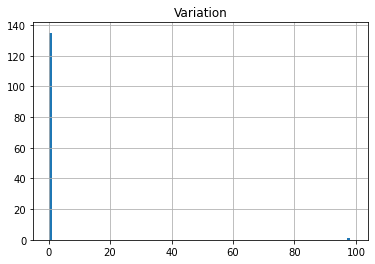
\includegraphics[width=0.7\linewidth]{figures/volume_plot}
\end{figure}

From the histograms it is clear how the value of 97.60, is far from general population. This doesn't mean it is necessarily wrong but it should make ring a bell in our head\ldots

To remove outliers from data we can either delete the entire row or just replace the suspicious values with a default (e.g. 0, 1, a threshold value\ldots).

\textbf{Note}: missing data may be informative itself~!~When filling the gap with \emph{artificial data} (e.g. mean, median, std\ldots) having similar properties than real observation, the added value won't be scientifically valid, no matter how sophisticated your filling method is.

\begin{ipythonnon}
import numpy as np

df2 = df2.replace(11902, 500) # replace 11902 with 500
df2 = df2.replace(11902, np.nan) # replace 11902 with NaN
df2 = df2.mask(df1 >= 150, 5) # replace every element >=600 with 5
\end{ipythonnon}

\subsection{Handle Missing Data}\label{handle-missing-data}

Usually when importing data with \texttt{pandas} we may have some NaN values. Like for the outliers we can use the \texttt{replace} or \texttt{mask} methods to remove the NaNs. In case the whole row as NaN it may be wise to drop it entirely.

Additionally we can use \texttt{dropna()} which remove all the NaN in the dataframe at once.

\begin{ipythonnon}
df1 = df1.dropna()
print (f"Number of rows after dropping NaN: {len(df1)}")
\end{ipythonnon}
\begin{ioutput}
Number of rows after dropping NaN: 242
\end{ioutput}

\subsection{Filter, Sort and Clean Data}
\label{filter-sort-and-clean-data}

\subsubsection{Filtering}\label{filtering}

When we work with huge datasets we may reach computational limits (e.g. insufficient memory, CPU performance, too slow processing time\ldots) and in those cases it can be helpful to filter data by attributes for example splitting by time or some other property.

Assuming to have the following table and putting back the volume column

\begin{ipythonnon}
# df.iloc[row, col]
# NOTE: iloc takes row and column index (two numbers)
# loc instead takes row index and column name

print (df1.iloc[1, 2]) # returns 62 the volume associated with the row
\end{ipythonnon}
\begin{ioutput}
111504800.0
\end{ioutput}

\begin{ipythonnon}
#df.iloc[row1:row2, col1:col2]
# this is called slicing, remember ?

print (df1.iloc[0:2, 2:3]) # returns rows 0 and 1 of column 2
\end{ipythonnon}
\begin{ioutput}
        Volume
1  101729600.0
2  111504800.0
\end{ioutput}

\begin{ipythonnon}
subset = df1.iloc[:, 1] # select column 1
subset = df1.iloc[2, :] # select row 2
subset = df1.iloc[0:2, :] # select 2 rows
subset = df1.iloc[:2, :] # this is equivalent to before
\end{ipythonnon}

A more advanced way of filtering is the following (it applies a selection on the values). The notation is a bit awkward but very useful:

\begin{ipythonnon}
import datetime

# colon means all the rows
subset = df1[df1.iloc[:, 0] < datetime.datetime(2020, 8, 15)]
print (subset)
\end{ipythonnon}
\begin{ioutput}
         Date       Price       Volume  Variation
1  2020-05-19   78.285004  101729600.0  -0.005778
2  2020-05-20   79.807503  111504800.0   0.019448
3  2020-05-21   79.212502  102688800.0  -0.007455
5  2020-05-22   79.722504   81803200.0   0.006438
6  2020-05-26   79.182503  125522000.0  -0.006774
..        ...         ...          ...        ...

[61 rows x 4 columns]
\end{ioutput}

\subsubsection{Sorting}\label{sorting}

To sort data we can use \texttt{sort\_values()} method (it can be specified ascending, descending).

\begin{ipythonnon}
# sort by price then by date in descending order
print (df2.sort_values(by=['Price', "Date"], ascending=False)[:5])
\end{ipythonnon}
\begin{ioutput}
                 Price
Date                  
26/01/2021  143.160004
25/01/2021  142.919998
27/01/2021  142.059998
22/01/2021  139.070007
04/02/2021  137.389999
\end{ioutput}
        
\subsubsection{Cleaning or Regularizing}
\label{cleaning-or-regularizing}

As we will see when dealing with machine learning, often we need to regularize our data to improve the stability of a training. One typical situation is when we want to \emph{normalize} data, which means re-scale the values into a range of $[0, 1]$.

\begin{equation*}
\begin{gathered}
x = [1,43,65,23,4,57,87,45,45,23]\\
x_{new} = \cfrac{x - x_{min}}{x_{max} - x_{min}}\\
x_{new} = [0,0.48,0.74,0.25,0.03,0.65,1,0.51,0.51,0.25]
\end{gathered}
\end{equation*}

To apply such a transformation with \texttt{pandas} is very easy: 
\begin{ipythonnon}
df1['Price'] = (df1['Price'] - df1['Price'].min()) \
    / (df1['Price'].max() - df1['Price'].min())
print (df1.head())
\end{ipythonnon}
\begin{ioutput}
        Date     Price       Volume  Variation
1 2020-05-19  0.000000  101729600.0  -0.005778
2 2020-05-20  0.000129  111504800.0   0.019448
3 2020-05-21  0.000078  102688800.0  -0.007455
5 2020-05-22  0.000122   81803200.0   0.006438
6 2020-05-26  0.000076  125522000.0  -0.006774
\end{ioutput}
        
Another quite common transformation is called \emph{standardization}, essentially we re-scale data to have 0 mean and standard deviation of 1:

\begin{equation}
x_{new} = \cfrac{x-\mu}{\sigma}
\label{eq:standardization}
\end{equation}

Again it is straightforward to do it in \texttt{pandas}:

\begin{ipythonnon}
df1.hist('Volume', bins=np.arange(180, 220, 1))

print (df1['Volume'].mean())
print (df1['Volume'].std())
\end{ipythonnon}
\begin{ioutput}
128765806.61157025
53204829.93713034
\end{ioutput}

\begin{ipythonnon}
df1['Volume'] = (df1['Volume'] - df1['Volume'].mean()) / df1['Volume'].std()
df1.hist('Volume', bins=np.arange(-5, 5, 0.1))

print (df1['Volume'].mean())
print (df1['Volume'].std())
\end{ipythonnon}
\begin{ioutput}
-1.5598174726138563e-17
1.0
\end{ioutput}

Figure~\ref{fig:standardization} shows the comparison of the "volume" distribution before and after standardization.

\begin{figure}[htb]
	\centering
	\subfloat[Original.]{%
		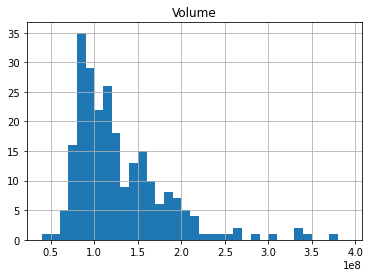
\includegraphics[width=0.45\textwidth]{figures/volume_plot_2}
	}
	\subfloat[Standardized according to Eq.~\ref{eq:standardization}.]{%
		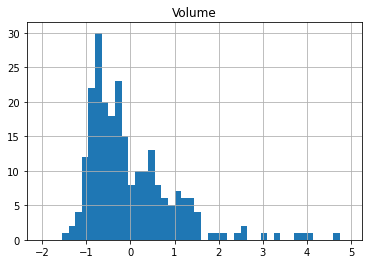
\includegraphics[width=0.45\textwidth]{figures/volume_plot_3}
	}
	\caption{Comparison between ``volume'' distributions.}
	\label{fig:standardization}
\end{figure}

\subsection{Operations on Data}
Using \texttt{pandas} all sorts of calculations between rows or columns can be made. Some example of that will be shown in the next Chapters, here just a simple application of Moving Average (MA) is described.

In finance, technical analysis is an analysis methodology for forecasting the direction of prices through the study of past market data, primarily price and volume. Technical analysts rely on a combination of technical indicators to study a stock and give insight about possible trading strategies. 

Consider for example a particular indicator called \emph{Bollinger Bands}. It is usually used to provide potential buy / sell signals and to define the prevailing high and low prices in a market to characterize the trading band of a financial instrument or commodity. You can think of Bollinger Bands as a volatility indicator. Bands consist of Moving Average lines, a upper band and lower band. The upper and lower bands are simply MA adding and subtracting standard deviation ($\sigma$), which is a sort of  measurement of volatility. 
\[
\begin{split}
\textrm{Upper Band} & = (\textrm{MA} + K\sigma)\\
\textrm{Lower Band} & = (\textrm{MA} - K\sigma)
\end{split}
\]

In the following example we are going to use a 20 day moving average and $K=2$. Imagine to have the historical series of AMZN stock closing prices. Bollinger Bands can be quickly and easily constructed as follows 

\begin{ipythonnon}
import yfinance as yf
import pandas as pd
import matplotlib.pyplot as plt

proxy = yf.Ticker('AMZN')
df = proxy.history(start='2017-04-02', end='2018-05-02')['Close']

# calculate Moving Average with 20 days window
ma = df.rolling(window=20).mean()

# calculate the standard deviation
rstd = df.rolling(window=20).std()

df['upper'] = ma + 2 * rstd
df['lower'] = ma - 2 * rstd

ax = df.plot(title='AMZN Price and Bollinger Bands', figsize=(10,8))
ax.fill_between(df.index, df['lower'], df['upper'], color='#ADCCFF', alpha='0.4')
ax.set_xlabel('date')
ax.set_ylabel('Price Moving Average')
ax.set_xlim('2017-05-02', '2018-05-02')
ax.grid()
\end{ipythonnon}

The resulting plot is shown in Fig.~\ref{fig:bollinger_bands} which can be interpreted by saying that approximately 90\% of prices lay between the two bands. If the stock price breaks out the upper band, it could be an overbought condition (indication of short). Similarly, when it breaks out the lower band, it could be oversold condition (indication of long). 

\begin{figure}[htb]
	\centering
	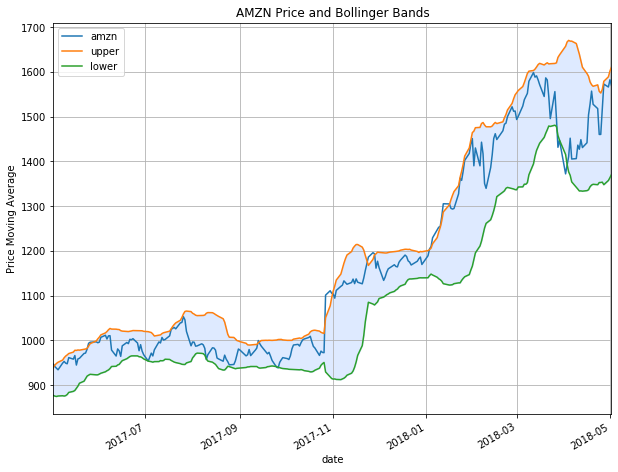
\includegraphics[width=0.7\textwidth]{figures/bollinger_bands}
	\caption{Bollinger Bands plot applied to AMZN historical prices.}
	\label{fig:bollinger_bands}
\end{figure}

\section{Plotting in \texttt{python}}\label{plotting-in-python}

As we have just seen \texttt{pandas} allows to quickly draw histograms of dataframe columns, but during an analysis we may want to plot distributions from \texttt{list} or objects not stored in a dataframe. Furthermore the simple although very useful interface doesn't grant full access to all plotting features that we need to produce nice and informative plots.

In order to do so we can use the \texttt{matplotlib} module which is specifically dedicated to plotting (\texttt{pandas} interface is based on the same module indeed). 

In the next Sections we will look briefly to its capabilities. For those interested a more detailed and comprehensive documentation can be found at~\cite{matplotlib}.

\subsection{Canvas}\label{canvas}

The first element we need to plot is a \emph{canvas}, the white rectangular space where we draw our data. \texttt{matplotlib} provides a default canvas if no specific command is given (a 640x480 pixels space) but you can customize it by specifying many different parameters, the most common are:

\begin{itemize}
\tightlist
\item \texttt{figsize}: width, height in inches. If not provided, defaults to \([6.4, 4.8]\);
\item \texttt{dpi}: resolution of the figure. If not provided, defaults to 100;
\item \texttt{facecolor}: the background color. If not provided, defaults to \texttt{'white'}, or \texttt{'w'}.
\end{itemize}

In the following example we create a canvas (8 inches x 5 inches) with a resolution of 80 dots per inches (dpi) and a green background color.

\begin{ipythonnon}
from matplotlib import pyplot as plt

fig = plt.figure(figsize=(8,5), dpi=80, facecolor='green')
\end{ipythonnon}

Once we have a canvas we cannot even draw it unless we have some plot to show. So let's see the most commonly used types of plot.

\subsection{Chart Object}\label{chart-object}

Below a concise list of the main chart objects that are used when presenting financial data.

\subsubsection{Histograms}\label{histograms}

A histogram is an approximate representation of the distribution of numerical data. To construct a histogram, the first step is to \emph{bin} (or \emph{bucket}) the range of values (i.e. divide the entire range of values into a series of intervals) and then count how many values fall into each interval.

If the bins are of equal size, a rectangle is erected over the bin with height proportional to the frequency (i.e. the number of cases in each bin).
However, bins do not need to be of equal width; in that case, the erected rectangle is defined to have its area proportional to the frequency of cases in the bin. 
The vertical axis is then not the frequency but frequency density (i.e. the number of cases per unit of the variable on the horizontal axis).

To create a histogram with \texttt{matplotlib} it is enough to pass a list (or a \texttt{numpy.array}) with data to represent to the function \texttt{hist} and then call \texttt{show()} to actually draw the plot (I have used the previously defined canvas just to show the results), Fig.~\ref{fig:histo1}.

\begin{ipythonnon}
y1 = [40.9, 47.7, 40.6, 43.0, 45.4, 42.3, 33.8, 49.6,
47.6, 52.3, 43.1, 36.5, 43.7, 52.4, 37.0, 42.4, 38.4, 39.9, 40.6, 35.7, 42.4,
38.3, 43.6, 38.5, 43.5, 42.9, 42.1, 39.8, 35.8, 44.1,
41.5, 42.6, 45.4, 38.6, 37.3, 37.8, 48.1, 44.8, 32.7, 40.3]

fig = plt.figure(figsize=(8,5), dpi=80, facecolor='green')
plt.hist(y1)
plt.show()
\end{ipythonnon}

\begin{figure}[htb]
	\centering
	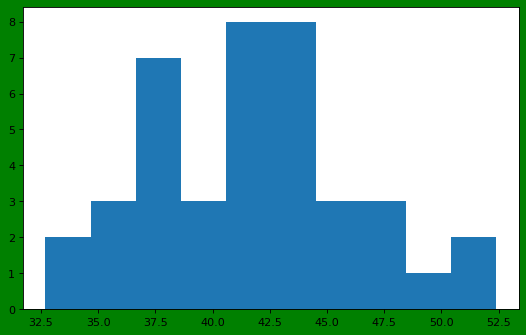
\includegraphics[width=0.7\textwidth]{figures/histo1}
	\caption{Example of histogram drawn on the previously defined canvas.}
	\label{fig:histo1}
\end{figure}

If you are not satisfied with the default binning and/or you want to change the range shown in the plot, those can be specified in the call to \texttt{hist} like this (see Fig.~\ref{fig:histo2})

\begin{ipythonnon}
# after data there is the number of equally spaced bins
# to be used, then the range

plt.hist(y, 50, range=(30, 50))
plt.show()
\end{ipythonnon}

\begin{figure}[htb]
	\centering
	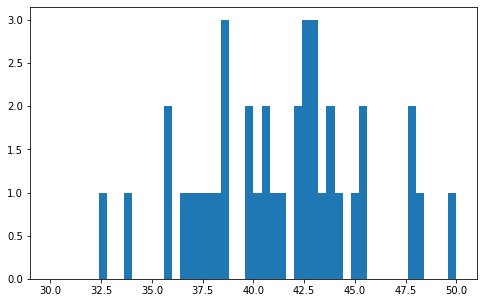
\includegraphics[width=0.7\textwidth]{figures/histo2}
	\caption{Example of histogram with custom binning and range.}
	\label{fig:histo2}
\end{figure}

Passing other parameters it is possible to modify the style of the
histogram, like its color which can be specified by name. For the basic built-in colors, you can also use a single letter

\begin{itemize}
\tightlist
\item b: blue
\item g: green
\item r: red
\item c: cyan
\item m: magenta
\item y: yellow
\item k: black
\item w: white
\end{itemize}

Plotting multiple histograms on the same canvas is as easy as calling various times \texttt{hist} (binning should be the same for each histogram though).

To each object that is plotted can be associated a label, passing the corresponding parameter to the object call, so that we can build a legend. Latex symbols can be used whenever text is used, the characters have to be enclosed between dollar symbols (i.e. \$\\mu\$). 
The legend will be shown on the canvas with the command  \texttt{legend()}.

A grid can be added to the plot with \texttt{plt.grid(True)} for a nicer look. Figure~\ref{fig:histo3} shows such an example.

\begin{ipythonnon}
y2 = [40.6, 40.5, 37.3, 37.6, 39.0, 38.5, 36.0, 
      39.0, 36.8, 41.4, 41.9, 39.9, 39.0, 37.7, 
      35.0, 37.9, 35.2, 39.5, 37.7, 38.4, 42.4, 
      38.1, 39.0, 34.7, 37.1, 36.6, 37.0, 40.8, 
      39.0, 41.5]

plt.hist(y1, 50, range=(30, 50), color='red', label='Red Hist')
plt.hist(y2, 50, range=(30, 50), color='yellow', label='Yellow Hist')
plt.legend()
plt.grid(True)
plt.show()
\end{ipythonnon}

\begin{figure}[htb]
	\centering
	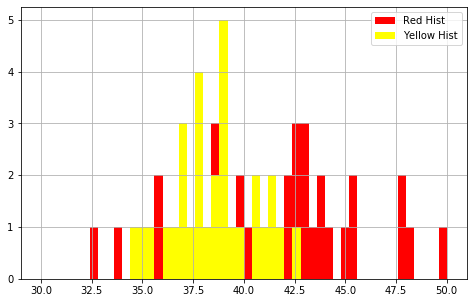
\includegraphics[width=0.7\textwidth]{figures/histo3}
	\caption{Plotting two histograms on the same canvas with different colors and the 
		corresponding legend.}
	\label{fig:histo3}
\end{figure}

\subsubsection{Scatter Plot}
\label{scatter}

A scatter plot uses Cartesian coordinates to display values of two variables that are connected (e.g. date and stock price). 

Data is displayed as a collection of points, each having the value of one variable determining the position on the horizontal axis and the value of the other variable determining the position on the vertical axis. If the points are coded (color/shape/size), one additional variable can be displayed.

To create such an object call \texttt{scatter} and pass the $x$ and $y$ lists, Fig.~\ref{fig:scatter1}.

\begin{ipythonnon}
y1 = [26.2, 5.4, 7.7, 3.8, 24.7, -5.5, 36.4, 12.9, 25.2, 21.0, 39.6,
      5.9, 24.8, 25.7, 42.3, 21.5, 32.3, 26.7, 37.4, 44.3, 29.0,
      52.9, 52.0, 49.5, 55.0, 40.7, 47.8, 41.1, 49.3, 58.8, 48.1,
      52.5, 51.1, 51.0, 54.3, 62.4, 52.8, 67.8, 83.6, 75.9]

x = range(len(y1))
plt.scatter(x, y1)
plt.show()
\end{ipythonnon}

\begin{figure}[htb]
	\centering
	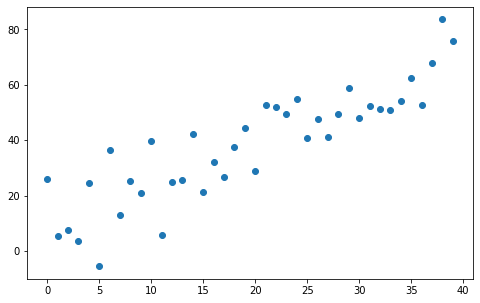
\includegraphics[width=0.7\textwidth]{figures/scatter}
	\caption{Example of scatter plot.}
	\label{fig:scatter1}
\end{figure}

Other parameters can be passed to \texttt{scatter}, the most useful are

\begin{itemize}
\tightlist
\item \texttt{label}: label the scatter plot for the legend;
\item \texttt{color}: set the color of the marker;
\item \texttt{marker}: set the style of the marker defined with a single character (+,*, o, x\ldots{});
\item \texttt{s=}: set the marker size.
\end{itemize}

And of course multiple scatter plot can be shown together in the same canvas calling \texttt{scatter} accordingly (see Fig.~\ref{fig:scatter2}).

\begin{ipythonnon}
y2 = [22.2, 3.4, 7.7, 5.8, 28.7, 0.5, 44.4, 22.9, 37.2, 35.0, 55.6,
      23.9, 44.8, 47.7, 66.3, 47.5, 60.3, 56.7, 69.4, 78.3, 65.0,
      90.9, 92.0, 91.5, 99.0, 86.7, 95.8, 91.1, 101.3, 112.8,
      104.1, 110.5, 111.1, 113.0, 118.3, 128.4, 120.8, 137.8, 155.6, 149.9]

plt.scatter(range(len(y1)), y1, s=10, marker="o",
color="lightblue", label="1st Scatter")
plt.scatter(range(len(y2)), y2, s=30, marker="*",
color="brown", label="2nd Scatter")
plt.legend()
plt.show()
\end{ipythonnon}

\begin{figure}[htb]
	\centering
	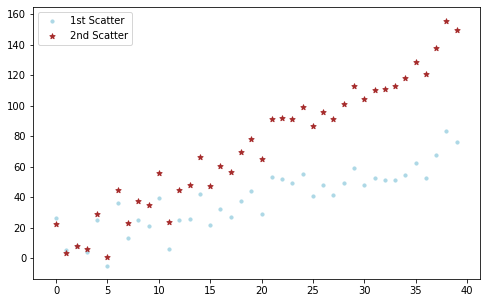
\includegraphics[width=0.65\textwidth]{figures/scatter2}
	\caption{More advanced scatter plot example.}
	\label{fig:scatter2}
\end{figure}

\subsubsection{Plot}\label{plot}

If you want to still plot $x$ and $y$ points but they should be connected with a line you can use the function \texttt{plot}. It acts similarly to \texttt{scatter} but the graphical result will be different.

Below the previous two scatter plots are plotted using \texttt{plot}, Figure~\ref{fig:plot1}

\begin{ipythonnon}
plt.plot(x, y1, label="1st Plot")
plt.plot(x, y2, label="2nd Plot")
plt.legend()
plt.show()
\end{ipythonnon}

\begin{figure}[htb]
	\centering
	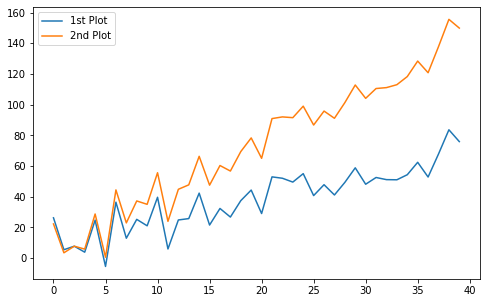
\includegraphics[width=0.65\textwidth]{figures/plot1}
	\caption{Example of scatter plot where points are connected by a line.}
	\label{fig:plot1}
\end{figure}

In this case the parameters allow to control the line style and the possibility to add the marker at each point (see Fig.~\ref{fig:plot2})

\begin{itemize}
\tightlist
\item \texttt{label}: label the scatter plot fot the legend;
\item \texttt{color}: set the color of the marker and the line;
\item \texttt{marker}: set the sityle of the marker defined with a single character (+,*, o, x\ldots{});
\item \texttt{s}: set the size of the marker;
\item \texttt{linestyle}: style of the line (`-', `--', `-.', `:');
\item \texttt{linewidth}: thickness of the line.
\end{itemize}

\begin{ipythonnon}
plt.plot(x, y1, marker="+", linestyle=":", color="darkgreen", label="1st Plot")
plt.plot(x, y2, marker="x", linewidth=5, color="pink", label="2nd Plot")
plt.legend()
plt.show()
\end{ipythonnon}

\begin{figure}[htb]
	\centering
	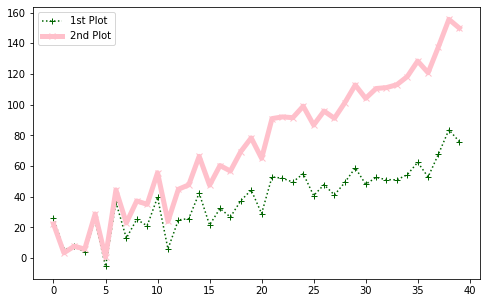
\includegraphics[width=0.7\textwidth]{figures/plot2}
	\caption{More refined example of connected scatter plot.}
	\label{fig:plot2}
\end{figure}

\subsubsection{Plotting a Function}\label{plotting-a-function}

Functions can be plotted using the \texttt{plot} method as well. They can be both functions from \texttt{python} modules or user-defined.

As an example let's try to plot $\mathrm{sin}(x/2)$; Figure~\ref{fig:sinx_x} reports the result of the code below.

\begin{ipythonnon}
from numpy import arange, sin

def func(x):
    return sin(x/2)
xs = arange(-10, 10, 0.01)

fig = plt.figure(figsize=(8,5))
plt.plot(xs, func(xs))
plt.show()
\end{ipythonnon}

\begin{figure}[htb]
	\centering
	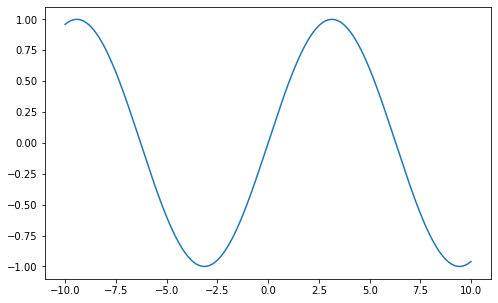
\includegraphics[width=0.65\textwidth]{figures/sinx_x}
	\caption{Example of a plot of a function, in this case \(\mathrm{sin}(x/2)\).}
	\label{fig:sinx_x}
\end{figure}

\subsection{Axes}\label{axes}

The axis of any plot can be formatted with many options.
First of all its range can be controlled with \texttt{xlim(min, max} and \texttt{ylim(min, max}. Then labels can be added with \texttt{xlabel(myLabel)} and \texttt{ylabel(myLabel)} (a global title to the plot can also be specified with \texttt{plt.title(myTitle)}).

Referring to the previous example we can write

\begin{ipythonnon}
fig = plt.figure(figsize=(8,5))
plt.plot(x, y1, marker="+", linestyle=":", color="darkgreen", label="1st Plot")
plt.plot(x, y2, marker="x", linewidth=5, color="pink", label="2nd Plot")
plt.title("Plot Title")
plt.xlabel("x label")
plt.ylabel("y label")
plt.legend()
plt.show()
\end{ipythonnon}
\noindent
and see the result in Fig.~\ref{fig:axis1}.

\begin{figure}[htb]
	\centering
	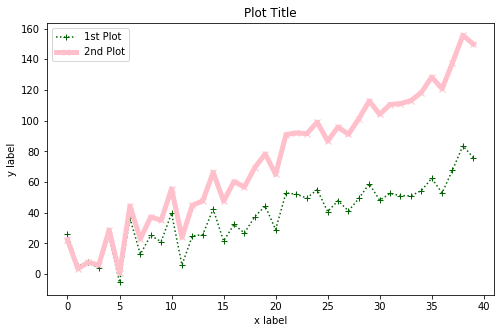
\includegraphics[width=0.65\textwidth]{figures/axis1}
	\caption{Improving the look of a plot by formatting the axis.}
	\label{fig:axis1}
\end{figure}

It can also be specified if axis has to be in linear or log scale with \texttt{xscale("log")} and/or \texttt{yscale("log")}, see Fig.~\ref{fig:axis2}.

\begin{ipythonnon}
fig = plt.figure(figsize=(8,5))
plt.plot(x, y1, marker="+", linestyle=":", color="darkgreen", label="1st Plot")
plt.plot(x, y2, marker="x", linewidth=5, color="pink", label="2nd Plot")
plt.title("Plot Title")
plt.xlabel("x label")
plt.ylabel("y label")
plt.xscale("log")
plt.yscale("log")
plt.legend()
plt.show()
\end{ipythonnon}

\begin{figure}[htb]
	\centering
	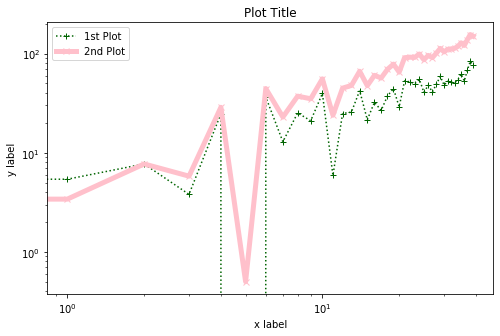
\includegraphics[width=0.7\textwidth]{figures/axis2}
	\caption{Example of log-scale plot.}
	\label{fig:axis2}
\end{figure}

\subsubsection{Date on Axis}\label{date-on-axis}

A special need, very common in finance, is to have dates on the $x$ axis. This can be done like shown in the next example and in Figure~\ref{fig:axis3}:

\begin{ipythonnon}
import datetime as dt
import matplotlib.dates as mdates

dates = ['01/02/1991','01/03/1991','01/04/1991']
xd = [dt.datetime.strptime(d,'%m/%d/%Y').date() for d in dates]
yd = range(len(xd))
fig = plt.figure(figsize=(8,5))
plt.gca().xaxis.set_major_formatter(mdates.DateFormatter('%m/%d/%Y'))
plt.gca().xaxis.set_major_locator(mdates.DayLocator())
plt.plot(xd, yd)
plt.gcf().autofmt_xdate() # this makes a prettier formatting
plt.show()
\end{ipythonnon}

\begin{figure}[ht]
	\centering
	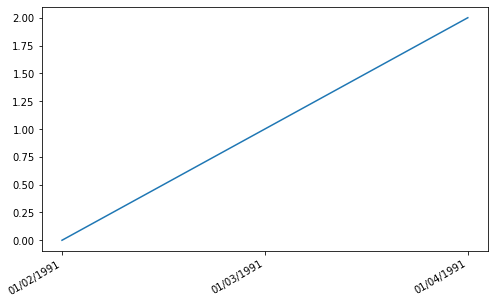
\includegraphics[width=0.6\textwidth]{figures/axis3}
	\caption{Plotting with dates on the $x$ axis.}
	\label{fig:axis3}
\end{figure}

\subsection{Subplots}
\label{subplots}

It may happen that we need to plot two or more plots side by side or in a grid fashion.

Then the canvas can be split into sub-canvases with the  \texttt{subplot} commands which takes in input the number of rows, columns and the index of the current subplot. It returns the \emph{sub-canvas} object that can be used to draw like previously shown.

There is one complication though, some of the commands change when
dealing with subplots: \texttt{xlabel} and \texttt{ylabel} for example becomes \texttt{set\_xlabel} and \texttt{set\_ylabel}. Similarly for \texttt{xlim} and \texttt{ylim}.

As an example imagine that we want to plot previous data side by side on two canvases instead of together in the same (Fig.~\ref{fig:subplot})

\begin{ipythonnon}
fig = plt.figure(figsize=(8,5))
sub1 = plt.subplot(1, 2, 1)
sub1.plot(x, y1, marker="+", linestyle=":", color="darkgreen", label="1st Plot")
sub1.set_xlabel("x label")
sub1.set_ylabel("y label")
sub1.legend()
sub2 = plt.subplot(1, 2, 2)
sub2.plot(x, y2, marker="x", linewidth=5, color="pink", label="2nd Plot")
sub2.set_xlabel("x label")
sub2.set_ylabel("y label")
sub2.legend()
plt.show()
\end{ipythonnon}

\begin{figure} [htb]
	\centering
	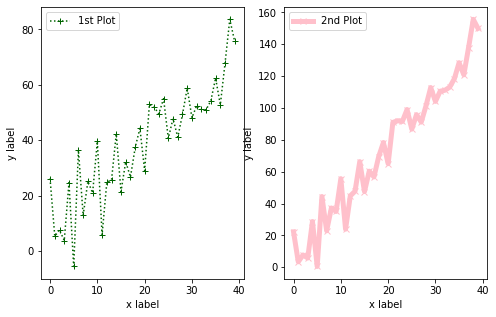
\includegraphics[width=0.65\textwidth]{figures/subplot}
	\caption{Example of subplots.}
	\label{fig:subplot}
\end{figure}

Subplots can also be arranged in another way like, see instead Figure~\ref{fig:subplot2}

\begin{ipythonnon}
fig = plt.figure(figsize=(8,5))
sub1 = plt.subplot(2, 1, 1)
sub1.plot(x, y1, marker="+", linestyle=":", color="darkgreen", label="1st Plot")
sub1.set_xlabel("x label")
sub1.set_ylabel("y label")
sub1.legend()
sub2 = plt.subplot(2, 1, 2)
sub2.plot(x, y2, marker="x", linewidth=5, color="pink", label="2nd Plot")
sub2.set_xlabel("x label")
sub2.set_ylabel("y label")
sub2.legend()
plt.show()
\end{ipythonnon}

%FIXME share the same axis xlabel plot 1 is covered
\begin{figure}[htbp]
	\centering
	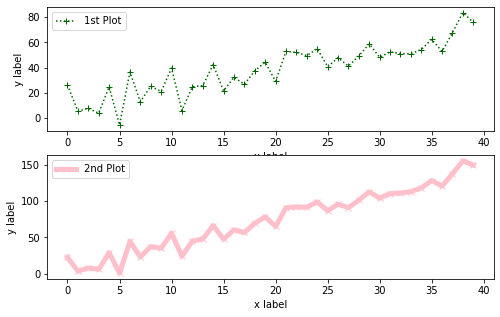
\includegraphics[width=0.65\textwidth]{figures/subplot2}
	\caption{Different arrangement of the two subplots.}
	\label{fig:subplot2}
\end{figure}

\subsection{Lines and Text}\label{lines-and-text}

To make plots more informative it can be useful to add text or lines on it.

\subsubsection{Lines}\label{lines}

Lines can be drawn with \texttt{hlines} (for horizontal lines) and
\texttt{vlines} (for vertical lines). The commands take in input the \texttt{y}, \texttt{x\_min}, \texttt{x\_max} and \texttt{x}, \texttt{y\_min}, \texttt{y\_max} respectively. Beware, coordinates are relative to the axis scale.

Other parameters allow to format the line in terms of color, style, width\ldots. Look for example at Fig.~\ref{fig:lines}

\begin{ipythonnon}
fig = plt.figure(figsize=(8,5))
plt.plot(x, y1, marker="+", linestyle=":", color="darkgreen", label="1st Plot")
plt.plot(x, y2, marker="x", linewidth=5, color="pink", label="2nd Plot")
plt.title("Plot Title")
plt.xlabel("x label")
plt.ylabel("y label")
plt.hlines(65, 0, 37.5, color='red', linestyle="-.", label='Critical Thr.')
plt.legend()
plt.show()
\end{ipythonnon}

\begin{figure}[htb]
	\centering
	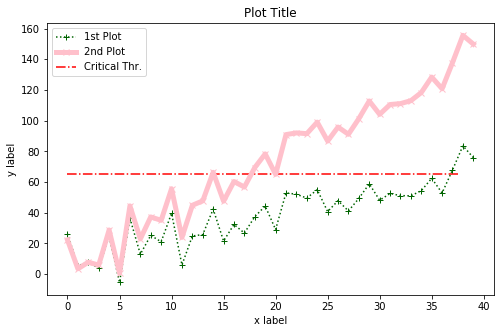
\includegraphics[width=0.7\textwidth]{figures/lines}
	\caption{Adding lines to our plots.}
	\label{fig:lines}
\end{figure}

Notice as the $y$ value is 65 and $x$ goes from 0 to 37.5 which corresponds to each axis.

Analogously for a vertical line, except that we have to first specify the $x$ value and then the $y$ range (Fig.~\ref{fig:lines2}).

\begin{ipythonnon}
fig = plt.figure(figsize=(8,5))
plt.plot(x, y1, marker="+", linestyle=":", color="darkgreen", label="1st Plot")
plt.plot(x, y2, marker="x", linewidth=5, color="pink", label="2nd Plot")
plt.title("Plot Title")
plt.xlabel("x label")
plt.ylabel("y label")
plt.vlines(22, 0, 120, color='gray', label='Splitting Thr.')
plt.legend()
plt.show()
\end{ipythonnon}

\begin{figure}[htb]
	\centering
	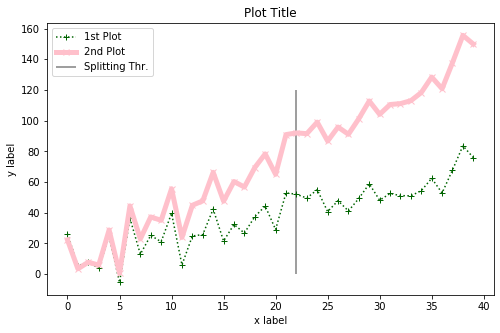
\includegraphics[width=0.7\textwidth]{figures/lines2}
	\caption{Vertical lines.}
	\label{fig:lines2}
\end{figure}

\subsubsection{Text}\label{text}

Like lines, text can be added to the plot with the command \texttt{text}.
This function takes the \texttt{x} and \texttt{y} coordinates of starting point and the actual text string. Like before coordinates are relative to the axis plot.

Other options can be used to format the text style, their meaning should be straightforward:

\begin{itemize}
\tightlist
\item \texttt{backgroundcolor};
\item \texttt{color};
\item \texttt{fontfamily}: (FONTNAME, `serif', `sans-serif', `cursive', `fantasy', `monospace');
\item \texttt{fontsize}; (size in points, `xx-small', `x-small', `small', `medium', `large', `x-large', `xx-large');
\item \texttt{fontstyle}: (`normal', `italic', `oblique');
\item \texttt{horizontalalignment}: (`center', `right', `left');
\item \texttt{rotation}: takes the angle in degrees;
\item \texttt{verticalalignment}: (`center', `top', `bottom', `baseline', `center\_baseline').
\end{itemize}

\begin{ipythonnon}
fig = plt.figure(figsize=(8,5))
plt.plot(x, y1, marker="+", linestyle=":", color="darkgreen", label="1st Plot")
plt.plot(x, y2, marker="x", linewidth=5, color="pink", label="2nd Plot")
plt.title("Plot Title")
plt.xlabel("x label")
plt.ylabel("y label")
plt.vlines(22, 0, 120, color='gray')
plt.text(23, 5, "Splitting Thr.", rotation=90)
plt.hlines(65, 0, 37.5, color='red', linestyle="-.")
plt.text(25, 75, "Critical Thr.", backgroundcolor="red", color="white")
plt.legend()
plt.show()
\end{ipythonnon}

\begin{figure}[htb]
	\centering
	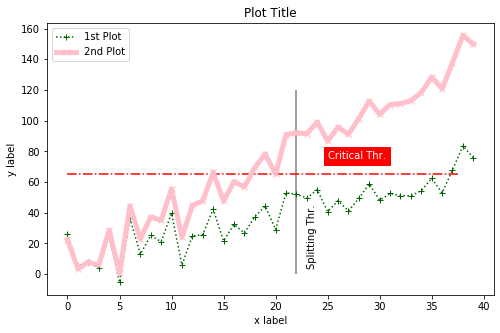
\includegraphics[width=0.7\textwidth]{figures/text}
	\caption{Adding also some text to our plot.}
	\label{fig:text}
\end{figure}

\subsection{Saving}\label{saving}

A plot can be saved into a file for later usage with \texttt{savefig} which takes in input the file name. The format of the file will be inferred from the file name extension (.jpg, .png, .gif\ldots)

\begin{ipythonnon}
plt.savefig("myfigure.png")
\end{ipythonnon}

\section*{Exercises}
\begin{question}
Using \texttt{pandas} import data stored in \href{https://github.com/matteosan1/finance_course/raw/master/input_files/stock_market.xlsx}{stock\_market.xlsx}. With the resulting dataframe:
\begin{itemize}
\tightlist
\item remove duplicates and missing data (how many rows are left ?);
\item find stocks with positive variation;
\item determine the five lowest price stocks.
\end{itemize}
\end{question}

\cprotEnv\begin{solution}
First load the excel file into a dataframe and look at data structure.

\begin{ipython}
import pandas as pd

df = pd.read_excel("stock_market.xlsx")
print (len(df))
print (df.head())
\end{ipython}
\begin{ioutput}
52
  ticker       Price  Volume     Delta    Delta%     Market Cap
0    APH   65.654160  1.5950 -0.078423 -0.001178   46649.495552
1    HRL   44.971874  3.3267 -1.120468 -0.024254   24457.936896
2    REG   49.253113  0.8656 -0.360996 -0.007412   11351.617536
3    BWA   43.179356  4.8792  1.734138  0.042629   10611.859456
4   INTU  410.860809  1.1647  8.171570  0.019976  115895.599104
\end{ioutput}
        
If we are not sure that data is \emph{clean} we should check for duplicates and \texttt{NaN} and take care of them. The \texttt{duplicated} method returns the status of each row (duplicate or not, True or False). If we would like just to see the duplicated entries we could combine the \texttt{duplicated} method with the selection syntax like this:

\begin{ipython}
print(df[df.duplicated() == True])
\end{ipython}
\begin{ioutput}
   ticker       Price   Volume     Delta    Delta%     Market Cap
39    WDC   67.300003   6.0131  1.090004  0.016624   13900.362752
49    HII  170.458679   0.4316 -0.926727 -0.005507    8680.606720
51   QCOM  139.125961  11.9372 -0.788132 -0.005541  149658.779648
\end{ioutput}
        
So it looks like we have three duplicates and we can remove them:

\begin{ipython}
print ("Before duplicates removal: {}".format(len(df)))
df.drop_duplicates(inplace=True)
print ("After duplicates removal: {}".format(len(df)))
\end{ipython}
\begin{ioutput}
Before duplicates removal: 52
After duplicates removal: 49
\end{ioutput}

Then we need to take care of the \texttt{NaN}, again if we want to check the rows with \texttt{NaN} we can select (here the syntax is a little bit more complicated since we need to use \texttt{any} to look for \texttt{NaN} in every column):

\begin{ipython}
print ()df[df.isna().any(axis=1)])
\end{ipython}
\begin{ioutput}
   ticker       Price  Volume     Delta    Delta%     Market Cap
36   ODFL  206.511932  0.3687       NaN -0.009519   35271.376896
41    AAP         NaN  1.5906  2.566040  0.017669    8747.030528
46    ABT  123.174004  3.1618 -0.203285       NaN  193658.322944
\end{ioutput}
        
Since we don't want to artificially modify our sample we just drop rows with \texttt{NaN}:

\begin{ipython}
print ("Before NaN removal: {}".format(len(df)))
df.dropna(inplace=True)
print ("After NaN removal: {}".format(len(df)))
\end{ipython}
\begin{ioutput}
Before NaN removal: 49
After NaN removal: 46
\end{ioutput}

The second point asks to determine the companies with a daily positive variation. Clearly we have to apply to the dataframe a selection on the "Delta" (or "Delta\%") column requiring positive values.

\begin{ipython}
pos_var = df.loc[df["Delta"] > 0, :]
print (len(pos_var))
print (pos_var.head())
\end{ipython}
\begin{ioutput}
25
   ticker       Price   Volume     Delta    Delta%     Market Cap
3     BWA   43.179356  4.87920  1.734138  0.042629   10611.859456
4    INTU  410.860809  1.16470  8.171570  0.019976  115895.599104
5     RJF   75.888489  0.91605  2.174728  0.029352   24506.064896
6     CSX   29.297924  9.96330  0.198599  0.006767   63387.660288
10   CTVA   44.009796  1.87760  0.890366  0.020509   45105.881088
\end{ioutput}
        
So in origin we had 46 stocks and 25 of them have a positive variation of its price.

The last question requires to print the five lowest price stocks. In this case it is enough to sort by price the dataframe (ascending) and then just select the first five entries.

\begin{ipython}
highest_price = df.sort_values(by=['Price'], ascending=True)[:5]
highest_price
\end{ipython}
\begin{ioutput}
   ticker      Price     Volume     Delta    Delta%     Market Cap
27     RF  18.772100   6.377100  0.618860  0.033742   21679.149056
28      T  19.063257  67.769867  0.109594  0.005903  142539.997184
7     NWS  22.469374   0.901300 -0.294357 -0.012766   11940.613120
13    HWM  28.521683   1.581600  0.099586  0.003536   16887.724032
6     CSX  29.297924   9.963300  0.198599  0.006767   63387.660288
\end{ioutput}
\end{solution}

\begin{question}
Given the discount factors in \href{https://raw.githubusercontent.com/matteosan1/finance_course/master/input_files/exercise_5.28.csv}{exercise\_5.28.csv} plot the resulting discount curve, possibly adding axis labels and legend.
\end{question}

\cprotEnv\begin{solution}
\begin{ipython}
import pandas as pf
from datetime import date
from matplotlib import pyplot as plt
import matplotlib.dates as mdates

df = pd.read_csv("exercise_5.28.csv")
print (df.head())
dfs = df['dfs']
pillars = [d.date() for d in pd.to_datetime(df['pillars'])]

plt.plot(pillars, dfs, marker="o", label="EUR6M d.f.")

plt.gca().xaxis.set_major_formatter(mdates.DateFormatter('%Y-%m-%d'))
# this one instead rotate labels to avoid superimposition
plt.xticks(rotation=45)
plt.xlabel("Pillar dates")
plt.ylabel("Discount Factors")
plt.grid(True)
plt.legend()
plt.show()
\end{ipython}

\begin{figure}[htb]
\begin{center}
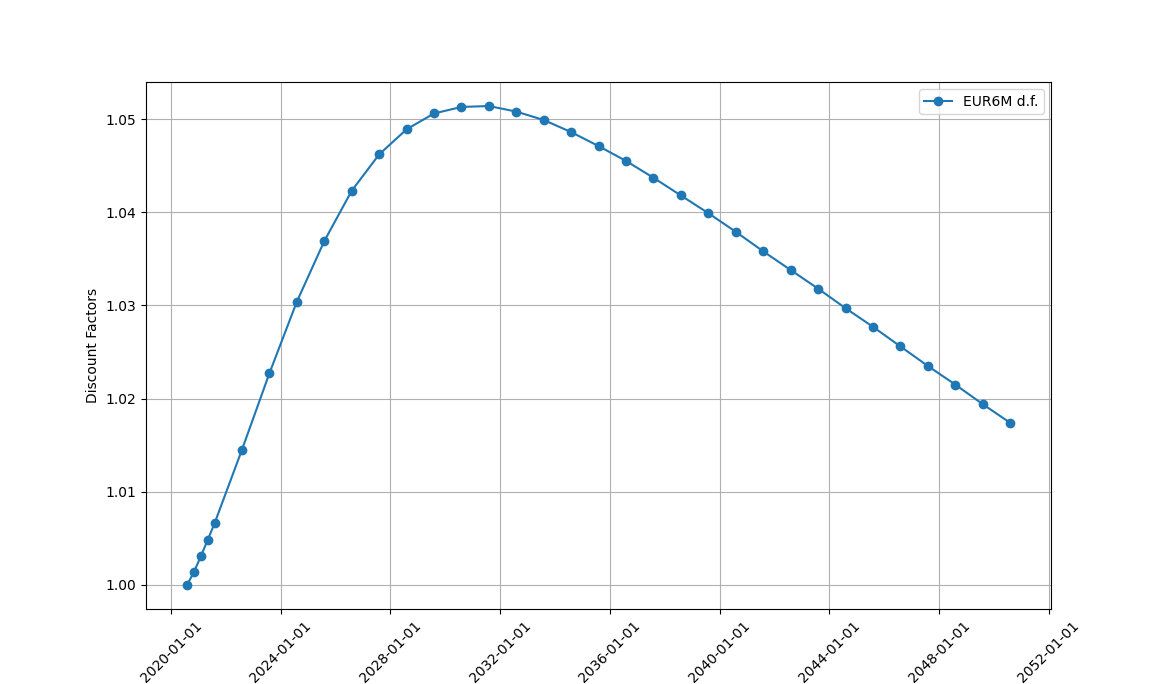
\includegraphics[width=0.7\linewidth]{figures/ex5.5}
\end{center}
\end{figure}
\end{solution}




 % da riguardare
\chapter{Matrices}
\label{sec:matrices}

In mathematics, a matrix is a rectangular array of numbers, symbols, or expressions, arranged in rows and columns. Matrices are commonly written in box brackets. The horizontal and vertical lines of entries in a matrix are called rows and columns, respectively. The size of a matrix is defined by the number of rows and columns that it contains. A matrix with $m$ rows and $n$ columns is called an $m\times n$ matrix or $m$-by-$n$ matrix, while $m$ and $n$ are called its dimensions. The dimensions of the following matrix are $2\times 3$ (read "two by three"), because there are two rows and three columns.

\begin{equation*}
\begin{bmatrix}
1 & 2 & 3\\
4 & 5 & 6
\end{bmatrix}
\end{equation*}

The individual items (numbers, symbols or expressions) in a matrix are called its elements or entries. 
In \texttt{python} matrices can be represented as \texttt{numpy.array}, so the example above will become:

\begin{ipython}
import numpy as np

print (np.array([[1, 2, 3],[4, 5, 6]]))
\end{ipython}
\begin{ioutput}
[[1 2 3]
 [4 5 6]]
\end{ioutput}

Essentially a \texttt{numpy.array} is a list of lists each one representing a matrix row. Arrays can have any dimension so they can be used to represent also vectors in \texttt{python}. There are two special types of arrays: \texttt{zeros} and \texttt{ones} whose names already clarify their nature.

\begin{ipython}
A = np.zeros(shape=(3, 3))
B = np.ones(shape+(4, 4))

print (A)
print (B)
\end{ipython}
\begin{ioutput}
[[0. 0. 0.]
 [0. 0. 0.]
 [0. 0. 0.]]

[[1. 1. 1. 1.]
 [1. 1. 1. 1.]
 [1. 1. 1. 1.]
 [1. 1. 1. 1.]]
\end{ioutput}

\section{Transpose of a Matrix}
The transpose of a matrix $[A]$, denoted by $[A^T]$, may be constructed by writing the rows of $[A]$ as the columns of $[A^T]$
and the columns of $[A]$ as the rows of $[A^T]$.
Formally, the $i$-th row, $j$-th column element of $[A^T]$ is the $j$-th row, $i$-th column element of $[A]$:

\begin{equation}[A^T]_{ij} = [A]_{ji}\end{equation}

If $[A]$ is an $m\times n$ matrix, then $[A^T]$ is an $n\times m$ matrix. 
As an example the transpose of:

\begin{equation*}
\begin{bmatrix}
1 & 5 & 3 \\
2 & -3 & 8
\end{bmatrix}
\quad \mathrm{is} \quad
\begin{bmatrix}
1 & 2 \\
5 & -3 \\
3  & 8
\end{bmatrix}
\end{equation*}

\section{Operation with Matrices}
\subsection{Adding and Subtracting Matrices}\label{adding-and-subtracting-matrices}

Usually matrices are used to list data or to represent system of equations. Since the entries are numbers, numerical operations can be performed on matrices. Indeed matrices can be added or subtracted by adding or subtracting corresponding entries.

In order to do this, the entries must correspond, therefore, addition and subtraction of matrices is only possible when the matrices have the
same dimensions.

Adding two matrices is very simple. Just add each element in the first matrix to the corresponding element in the second matrix.

\begin{equation*}
\begin{bmatrix}
1 & 2 & 3 \\
4 & 5 & 6
\end{bmatrix}
+
\begin{bmatrix}
10 & 20 & 30\\
40 & 50 & 60
\end{bmatrix}
=
\begin{bmatrix}
11 & 22 & 33\\
44 & 55 & 66
\end{bmatrix}
\end{equation*}
As you might guess, subtracting works the same way except that you subtract instead of adding.

\begin{equation*}
\begin{bmatrix}
10 & 20 & 30\\
40 & 50 & 60
\end{bmatrix}
-
\begin{bmatrix}
1 & 2 & 3 \\
4 & 5 & 6
\end{bmatrix}
=
\begin{bmatrix}
9 & 18 & 27\\
36 & 45 & 54
\end{bmatrix}
\end{equation*}
Adding and subtracting \texttt{numpy.array} is as easy as that:

\begin{ipython}
A = np.array([[1, 2, 3],[4, 5, 6]]
B = np.array([[10, 20, 30],[40, 50, 60]]

print (A + B)
print (A - B)
\end{ipython}
\begin{ioutput}
[[11 22 33]
 [44 55 66]]
 
[[ 9 18 27]
 [36 45 54]]
\end{ioutput}

\subsection{Scalar Multiplication}\label{scalar-multiplication}

Multiplying a matrix by a scalar $c$ means you add the matrix to itself $c$ times, or simply multiply each element by that constant.

\begin{equation*}
3 \cdot
\begin{bmatrix}
1 & 2 & 3 \\
4 & 5 & 6
\end{bmatrix}
=
\begin{bmatrix}
3 & 6 & 9 \\
12 & 15 & 18
\end{bmatrix}
\end{equation*}
Scalar multiplication of \texttt{numpy.array} is:

\begin{ipython}
c = 3
A = np.array([[1, 2, 3],[4, 5, 6]]

print (c * A)
\end{ipython}
\begin{ioutput}
[[ 3  6  9]
 [12 15 18]]
\end{ioutput}

\subsection{Matrix Multiplication}\label{matrix-multiplication}

Matrix multiplication is multiplying every element of each row of the first matrix times every element of each column in the second matrix. Each entry of the resultant matrix is computed one at a time.

Let's see with an example: 
\begin{equation*} 
\begin{bmatrix}
1 & 2 \\
3 & 4
\end{bmatrix}
\cdot
\begin{bmatrix}
5 & 6 \\
7 & 8
\end{bmatrix}
= ?
\end{equation*}
First ask: do the number of columns in the first matrix equal the number of rows in the second ? If so the product exists. Then start with producing the product for the first row, first column element. Take the first row of the first matrix and multiply by the first column of the second like this:

\begin{equation*} 
\begin{bmatrix}
1 & 2 \\
3 & 4
\end{bmatrix}
\cdot
\begin{bmatrix}
5 & 6 \\
7 & 8
\end{bmatrix}
=
\begin{bmatrix}
(1\cdot 5) + (2\cdot 7) & X \\
X & X
\end{bmatrix}
\end{equation*}
Continue the pattern with the first row of the first matrix with the second column of the second matrix:

\begin{equation*} 
\begin{bmatrix}
1 & 2 \\
3 & 4
\end{bmatrix}
\cdot
\begin{bmatrix}
5 & 6 \\
7 & 8
\end{bmatrix}
=
\begin{bmatrix}
(1\cdot 5) + (2\cdot 7) & (1\cdot 6) + (2\cdot 8)  \\
X & X
\end{bmatrix}
\end{equation*}
Then do the same with the second row of the first matrix and you are done:

\begin{equation*} 
\begin{bmatrix}
1 & 2 \\
3 & 4
\end{bmatrix}
\cdot
\begin{bmatrix}
5 & 6 \\
7 & 8
\end{bmatrix}
=
\begin{bmatrix}
(1\cdot 5) + (2\cdot 7) & (1\cdot 6) + (2\cdot 8)  \\
(3\cdot 5) + (4\cdot 7) & (3\cdot 6) + (4\cdot 8) 
\end{bmatrix}
=
\begin{bmatrix}
19 & 22 \\
43 & 50 
\end{bmatrix}
\end{equation*}
In \texttt{numpy} array multiplication can be done like this:

\begin{ipython}
A = np.array([[1, 2],[3, 4]]
B = np.array([[5, 6],[7, 8]]
	
print (np.dot(A, B))
# or equivalently A.dot(B)
\end{ipython}
\begin{ioutput}
[[19 22]
 [43 50]]
\end{ioutput}

\section{The identity matrix}\label{the-identity-matrix}

$[I]$ is defined so that $[A][I]=[A]$, i.e.~it is the matrix version of multiplying a number by one. What matrix has this property? A first guess might be a matrix full of 1s, but that does not work:

\begin{equation*}
\begin{bmatrix}
1 & 2 \\
3 & 4
\end{bmatrix}
\begin{bmatrix}
1 & 1 \\
1 & 1
\end{bmatrix}
=
\begin{bmatrix}
3 & 3 \\
7 & 7
\end{bmatrix}
\end{equation*}
The matrix that does work is a diagonal stretch of 1s, with all other elements being 0:

\begin{equation*}
\begin{bmatrix}
1 & 2 \\
3 & 4
\end{bmatrix}
\begin{bmatrix}
1 & 0 \\
0 & 1
\end{bmatrix}
=
\begin{bmatrix}
1 & 2 \\
3 & 4
\end{bmatrix}
\end{equation*}
So $[I] = 
\begin{bmatrix}
1 & 0 \\
0 & 1
\end{bmatrix}
$ is the identity matrix for $2\times 2$ matrices. The \texttt{numpy} equivalent of the identity matrix is given by
\texttt{numpy.identity(n)} with \texttt{n} the dimension of the matrix. So for example:

\begin{ipython}
A = np.array([[1, 2],[3, 4]]
I = np.identity(2)	

print (A)
print (np.dot(A, I))
\end{ipython}
\begin{ioutput}
[[1 2]
 [3 4]]

[[1. 2.]
 [3. 4.]]
\end{ioutput}
    
\section{Matrix Decomposition}
\label{eigendecomposition}

Decomposing a matrix means to find a product of matrices that is equal to the initial matrix. In this Section the case of \emph{eigen-decomposition} is described, where the initial matrix is decomposed into the product of its \emph{eigenvectors} and \emph{eigenvalues}.
%Before all, let's see the link between matrices and linear
%transformation. Then, you'll learn what are eigenvectors and
%eigenvalues.

\subsection{Eigenvectors and eigenvalues}
\label{eigenvectors-and-eigenvalues}
%\subsection{Matrices as linear transformations}
%\label{matrices-as-linear-transformations}

You can think of matrices as linear transformations so some matrices will rotate your space, others will re-scale it. When a matrix is applied to a vector (apply here means calculate the dot product of the matrix with the vector), we end up with a transformed version of the vector.

Let's apply the matrix $[A]$ to a vector $\boldsymbol{v}$

\begin{ipython}
import numpy as np
from finmarkets import plotVectors
from matplotlib import pyplot as plt

A = np.array([[1, 3], [2, 2]])	
v = np.array([2, 1])
Av = A.dot(v)

plotVectors([v.flatten({}, Av.flatten()], cols=["1190FF", "FF9A13"])
plt.ylim(1, 4)
plt.xlim(1, 4)
\end{ipython}
\begin{ioutput}
(-1.0, 4.0)
\end{ioutput}

Figure~\ref{fig:matrix_as_transform} shows the effect of the application of the matrix to the vector, the new vector (orange) has a different direction than the original one (light blue).

\begin{figure}[htb]
	\centering
	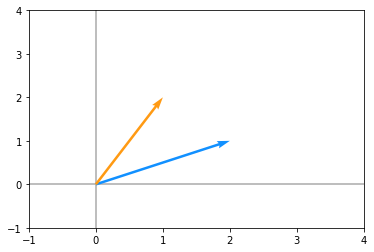
\includegraphics[width=0.7\linewidth]{figures/matrix_transformation}
	\caption{Application of a matrix to a vector, the new vector (orange) is different than the original one (blue).}
	\label{fig:matrix_as_transform}
\end{figure}


%We have seen an example of a vector transformed by a matrix. Now
%imagine that the transformation of the initial \%vector gives us a new
%vector that has the exact same direction. The scale can be different but
%the direction is the \%same. Applying the matrix doesn't change the
%direction of the vector. This special vector is called an eigenvector of
%\%the matrix.

Now imagine that the transformation of the initial vector by the matrix gives a new vector with the exact same direction. This vector is called an \emph{eigenvector} of $[A]$.

This means that \textbf{v} is a eigenvector of $[A]$ if \textbf{v} and $[A]\boldsymbol{v}$ (the transformed vector) have the same direction. The output vector is just a scaled version of the input one with the scaling factor $\lambda$ which is called an \emph{eigenvalue} of \([A]\). Mathematically, the following equation holds:

\begin{equation}
[A]\boldsymbol{v}=\lambda \boldsymbol{v}
\end{equation}

\subsection{Finding Eigenvalues and Eigenvectors in \texttt{python}}
\label{find-eigenvalues-and-eigenvectors-in-python}

\texttt{numpy} provides a function returning eigenvectors and eigenvalues: 

\begin{ipython}
A = np.array([[5, 1], [3, 3]])
np.linalg.eig(A)
\end{ipython}
\begin{ioutput}
(array([6., 2.]),

array([[ 0.70710678, -0.31622777],
       [ 0.70710678,  0.9486833 ]]))
\end{ioutput}
The eigenvectors correspond to the columns of the second array. This means that the eigenvector corresponding to \(\lambda=6\) is:

\begin{equation*}
\begin{bmatrix}
0.70710678 \\
0.70710678
\end{bmatrix}
\end{equation*}
while the eigenvector corresponding to $\lambda=2$ is:

\begin{equation*}
\begin{bmatrix}
−0.31622777 \\
0.9486833
\end{bmatrix}
\end{equation*}

It is important to note that there exists an infinite number of eigenvectors corresponding to a given eigenvalue, they are equivalent because they have the same direction but are just scaled differently. For example the first eigenvector found above is a scaled version of $\begin{bmatrix}1\\ 1\end{bmatrix}$.

\begin{ipython}
v = np.array([1, 2])
Av = A.dot(v)
v_np = [0.31622777, 0.9486833]	
\end{ipython}
\begin{ioutput}
(-1.0, 3.0)
\end{ioutput}
Figure~\ref{fig:eigenvectors} shows three equivalent eigenvectors found
with the code above. We can see that the vector found with \texttt{numpy} (in dark blue) is a scaled version of $\begin{bmatrix}1\\ -3\end{bmatrix}$.

\begin{figure}[htb]
	\centering
	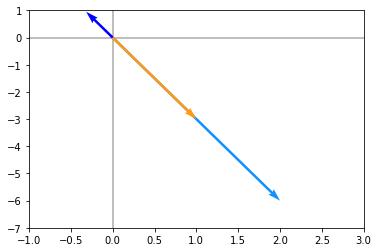
\includegraphics[width=0.7\linewidth]{figures/eigenvectors}
	\caption{Graphical representation of three equivalent eigenvectors.}
	\label{fig:eigenvectors}
\end{figure}

%Let's \([A]\) be the following matrix:
%
%\[A=\begin{bmatrix}
%5 &1 \\
%3 &3
%\end{bmatrix}\]
%
%We know that one eigenvector of A is:
%
%\[v=\begin{bmatrix}
%1 \\
%1\end{bmatrix}\] We can check that \([A]v=\lambda v\)
%
%\[\begin{bmatrix}
%5 & 1 \\
%3& 3\end{bmatrix}
%\begin{bmatrix}
%1 \\
%1\end{bmatrix}
%=\begin{bmatrix}
%6 \\
%6\end{bmatrix}\]
%
%We can represent \(v\) and \([A]v\) to check if their directions are the
%same:
%
%\begin{codebox}
%	\begin{Verbatim}[commandchars=\\\{\}]
%	\PY{n}{A} \PY{o}{=} \PY{n}{np}\PY{o}{.}\PY{n}{array}\PY{p}{(}\PY{p}{[}\PY{p}{[}\PY{l+m+mi}{5}\PY{p}{,} \PY{l+m+mi}{1}\PY{p}{]}\PY{p}{,} \PY{p}{[}\PY{l+m+mi}{3}\PY{p}{,} \PY{l+m+mi}{3}\PY{p}{]}\PY{p}{]}\PY{p}{)}
%	\PY{n}{v} \PY{o}{=} \PY{n}{np}\PY{o}{.}\PY{n}{array}\PY{p}{(}\PY{p}{[}\PY{p}{[}\PY{l+m+mi}{1}\PY{p}{]}\PY{p}{,} \PY{p}{[}\PY{l+m+mi}{1}\PY{p}{]}\PY{p}{]}\PY{p}{)}
%	
%	\PY{n}{Av} \PY{o}{=} \PY{n}{A}\PY{o}{.}\PY{n}{dot}\PY{p}{(}\PY{n}{v}\PY{p}{)}
%	
%	\PY{n}{orange} \PY{o}{=} \PY{l+s+s1}{\PYZsq{}}\PY{l+s+s1}{\PYZsh{}FF9A13}\PY{l+s+s1}{\PYZsq{}}
%	\PY{n}{blue} \PY{o}{=} \PY{l+s+s1}{\PYZsq{}}\PY{l+s+s1}{\PYZsh{}1190FF}\PY{l+s+s1}{\PYZsq{}}
%	
%	\PY{n}{plotVectors}\PY{p}{(}\PY{p}{[}\PY{n}{Av}\PY{o}{.}\PY{n}{flatten}\PY{p}{(}\PY{p}{)}\PY{p}{,} \PY{n}{v}\PY{o}{.}\PY{n}{flatten}\PY{p}{(}\PY{p}{)}\PY{p}{]}\PY{p}{,} \PY{n}{cols}\PY{o}{=}\PY{p}{[}\PY{n}{blue}\PY{p}{,} \PY{n}{orange}\PY{p}{]}\PY{p}{)}
%	\PY{n}{plt}\PY{o}{.}\PY{n}{ylim}\PY{p}{(}\PY{o}{\PYZhy{}}\PY{l+m+mi}{1}\PY{p}{,} \PY{l+m+mi}{7}\PY{p}{)}
%	\PY{n}{plt}\PY{o}{.}\PY{n}{xlim}\PY{p}{(}\PY{o}{\PYZhy{}}\PY{l+m+mi}{1}\PY{p}{,} \PY{l+m+mi}{7}\PY{p}{)}
%
%(-1.0, 7.0)
%\end{Verbatim}
%\end{codebox}
%
%\begin{center}
%	\adjustimage{max size={0.9\linewidth}{0.9\paperheight}}{eigenvectors_files/eigenvectors_3_1.png}
%\end{center}
%
%We can see that their directions are the same!
%
%This example shows that the eigenvectors \(v\) are vectors that change
%only in scale when we apply the matrix \([A]\) to them.

\section{The Inverse of a Matrix}\label{the-inverse-of-a-matrix}

The inverse of matrix $[A]$ is $[A^{-1}]$, and is defined by the property:

\begin{equation} 
[A][A^{-1}]=[I] 
\end{equation}

Hence the matrix $[B]$ is the inverse of the matrix $[A]$ if when multiplied together, $[A][B]$ gives the identity matrix. 
Using the definition let's try to find the inverse of:

\begin{equation*}
\begin{bmatrix}
3 & 4\\
5 & 6
\end{bmatrix}
\end{equation*}
First, let the following be true:

\begin{equation*}
\begin{bmatrix}
3 & 4\\
5 & 6
\end{bmatrix}
\begin{bmatrix}
a & b\\
c & d
\end{bmatrix}
=
\begin{bmatrix}
1 & 0\\
0 & 1
\end{bmatrix}
\end{equation*}
When multiplying this mystery matrix by our original matrix, the result is

\begin{equation*}
\begin{bmatrix}
3a+4c & 3b+4d\\
5a+6c & 5b+6d
\end{bmatrix}
=
\begin{bmatrix}
1 & 0\\
0 & 1
\end{bmatrix}
\end{equation*}
For two matrices to be equal, every element on the left must equal its corresponding element on the right. So, for these two matrices to equal each other:

\begin{equation*}
\begin{cases}
3a+4c=1\\
3b+4d=0\\
5a+6c=0\\
5b+6d=1
\end{cases}
\end{equation*}
Solving this simple system we get the following result:

\begin{equation*}
\begin{cases}
a=−3\\
b=2\\
c=2.5\\
d=−1.5
\end{cases}
\end{equation*}
Having solved for the four variables, the result is the inverse

\begin{equation*}
\begin{bmatrix}
−3 & 2\\
2.5 & −1.5
\end{bmatrix}
\end{equation*}
The quick check to be sure the result is correct is done in \texttt{python}. The \texttt{linalg.inv()} function can be used to find the inverse of a matrix:

\begin{ipython}
from numpy.linalg import inv

A = np.array([[3, 4],[5, 6]])	
print (inv(A))
\end{ipython}
\begin{ioutput}
[[-3.   2. ]
 [ 2.5 -1.5]]
\end{ioutput}

\subsection{The Moore-Penrose Pseudo-inverse}
\label{sec:the-moore-penrose-pseudoinverse}

%The Moore-Penrose pseudo-inverse is a direct application of the SVD. But
%before all, we have to remind that systems of equations can be expressed
%under the matrix form.
The Moore-Penrose pseudo-inverse is $[A^+]$ such as:

\begin{equation*}
[A][A^+]≈[I]
\end{equation*}

Think of it as a generalization of the inverse. It is defined for all matrices, but has fewer guaranteed properties as a result. For example, it will be a matrix such that $[𝐴][𝐴^+][𝐴]=[𝐴]$, but not necessarily the stronger usual inverse property is true $[𝐴^{−1}][𝐴]=[𝐴][𝐴^{−1}]=[𝐼]$ (the second one implies the first). In the special case where a matrix has an inverse, it will be the same as the pseudo-inverse.

%So pinv() gives you the inverse where it exists, and still gives
%something inverse-like everywhere else.

%The pseudo-inverse is the ``closest'' answer to \([𝐴]\boldsymbol{x}=[𝐼]\), in the sense that the norm \(||[𝐴][𝑋]−[𝐼]||_2\) is smallest. It's 0 when the
%inverse exists of course.

Let's create a non square matrix $[A]$, calculate its singular value decomposition and its pseudo-inverse with \texttt{linalg.pinv()}.

\begin{equation*}
A=\begin{bmatrix}
7&2\\
3&4\\
5&3
\end{bmatrix}
\end{equation*}

\begin{ipython}
A = np.array([[7, 2, 3],[4, 5, 3]])
A = np.linalg.pinv(A)
A_plus = np.linalg.pinv(A)
print (A_plus)
\end{ipython}
\begin{ioutput}
[[ 0.16666667 -0.10606061  0.03030303]
 [-0.16666667  0.28787879  0.06060606]]
\end{ioutput}
It can be checked that it is really the near inverse of $[A]$ since we know that

\begin{equation*}
A^{+}][A]\approx[A^{−1}][A]=[I]
\end{equation*}

\begin{ipython}
A_plus.dot(A)
\end{ipython}
\begin{ioutput}
array([[1.00000000e+00, 2.35922393e-16],
       [3.33066907e-16, 1.00000000e+00]])
\end{ioutput}
This is almost the identity matrix~!~Another difference with respect to the real inverse is that $[A^+][A]≈[I]$ but $[A][A^+]\neq [I]$.

\subsection{Eigen-decomposition}
\label{concatenating-eigenvalues-and-eigenvectors}

Now that we have an idea of what eigenvectors and eigenvalues are, we can see how it can be used to decompose a matrix. 
The \emph{eigen-decomposition} is given by

\begin{equation}
[A]=[V]\cdot \textrm{diag}(\boldsymbol{\lambda})\cdot [V^{−1}]
\end{equation}
where the matrix $[V]$ is made by concatenating all eigenvectors of $[A]$ in each column (like in the second array returned by \texttt{np.linalg.eig(A))}, $\textrm{diag}(\boldsymbol{\lambda})$ is a diagonal matrix containing all the eigenvalues. Continuing with our example above we have

\begin{equation*}
V=\begin{bmatrix}
1 & 1 \\
1 &−3\end{bmatrix}\qquad 
\textrm{diag}(\boldsymbol{\lambda})=\begin{bmatrix}
6&0\\
0&2
\end{bmatrix}
\end{equation*} 
and the inverse matrix of $[V]$ can be calculated with \texttt{numpy}

\begin{ipython}
V = np.array([[1, 1], [1, 3]])
V_inv = np.linalg.inv(V)
print (V_inv)
\end{ipython}
\begin{ioutput}
array([[ 0.75,  0.25],
       [ 0.25, -0.25]])
\end{ioutput}

So let's plug it into our equation:

\begin{equation*} 
[V]\cdot\textrm{diag}(\boldsymbol{\lambda})\cdot [V^{−1}]=
\begin{bmatrix}
1 & 1 \\
1 &−3\end{bmatrix}
\begin{bmatrix}
6&0\\
0&2\end{bmatrix}
\begin{bmatrix}
0.75 & 0.25\\
0.25&-0.25 \end{bmatrix}
=\begin{bmatrix}
5 & 1\\
3& 3\end{bmatrix}
\end{equation*}

Let's check our result with \texttt{python}

\begin{ipython}
lambdas = np.diag([6, 2])	
V.dot(lambdas).dot(V_inv)
\end{ipython}
\begin{ioutput}
array([[5., 1.],
       [3., 3.]])
\end{ioutput}

\subsubsection{Real symmetric matrix}
\label{real-symmetric-matrix}

In the case of real symmetric matrices ($[A]=[A^T]$) the eigen-decomposition can be expressed as

\begin{equation}
[A]=[Q][\Lambda][Q^T]
\end{equation} 
where $[Q]$ is the matrix with eigenvectors as columns and $\Lambda$ is $\textrm{diag}(\boldsymbol{\lambda})$.

For that reason, it can be useful to use symmetric matrices! Let's do it now with \texttt{linalg} from \texttt{numpy}

\begin{ipython}
A = np.array([[6, 2], [2, 3]])

eigVals, eigVecs = np.linalg.eig(A)
eigVals = np.diag(eigVals)

print (eigVecs.dot(eigVals).dot(eigVecs.T))
\end{ipython}
\begin{ioutput}
array([[6., 2.],
       [2., 3.]])
\end{ioutput}

%\subsubsection{Quadratic form to matrix form}
%\label{quadratic-form-to-matrix-form}
%
%Let's have the following quadratic equation:
%
%\[f(x)=ax^2_1+(b+c)x_1x_2+dx^2_2\] These quadratic forms can be
%generated by matrices:
%
%\[f(x)=
%\begin{bmatrix}
%x_1 & x_2
%\end{bmatrix}
%\begin{bmatrix}
%a&b\\
%c&d
%\end{bmatrix}
%\begin{bmatrix}
%x_1\\
%x_2\end{bmatrix}
%=x^T[A]x\]
%
%\subsection{With the Principal Axes Theorem}
%\label{with-the-principal-axes-theorem}
%
%Actually there is a simpler way to do the change of variable. We can
%stay in the matrix form. Recall that we start with the form:
%
%\[f(x)=x^T[A]x\] The linear substitution can be wrote in these terms. We
%want replace the variables \(x\) by \(y\) that relates by:
%
%\[x=[P]y\] We want to find \([P]\) such as our new equation doesn't
%contain the cross terms. The first step is to replace that in the first
%equation:
%
%\[x^T[A]x=([P]y)^T[A]([P]y)=y^T([P]^T[A][P])y\] Can you see the how to
%transform the left hand side (\(x\)) into the right hand side (\(y\))?
%The substitution is done by replacing \([A]\) with \([P]^T[A][P]\). We
%also know that \([A]\) is symmetric and thus that there is a diagonal
%matrix \([D]\) containing the eigenvectors of \([A]\) and such as
%\([D]=[P]^T[A][P]\). We thus end up with:
%
%\[x^T[A]x=y^T[D]y\] All of this implies that we can use \([D]\) to
%simplify our quadratic equation and remove the cross terms. If you
%remember from example 2 we know that the eigenvalues of \([A]\) are:
%
%\[[D]=\begin{bmatrix}
%7 &0\\
%0 &2\end{bmatrix}\]
%
%\[x^T[A]x=y^T[D]y=y^T
%\begin{bmatrix}
%7 &0\\
%0 &2\end{bmatrix}y=
%\begin{bmatrix}y_1 & y_2\end{bmatrix}
%\begin{bmatrix}
%7 &0\\
%0 &2\end{bmatrix}
%\begin{bmatrix}y_1\\y_2\end{bmatrix}
%=\begin{bmatrix}7y_1+0y_2 & 0y_1+2y_2\end{bmatrix}
%\begin{bmatrix}y_1\\y_2\end{bmatrix}=7y^2_1+2y^2_2
%\]
%
%This form (without cross-term) is called the principal axes form.
%
%\subsection{Quadratic form optimization}
%\label{quadratic-form-optimization}
%
%Depending to the context, optimizing a function means finding its
%maximum or its minimum. It is for instance widely used to minimize the
%error of cost functions in machine learning.
%
%Here we will see how eigendecomposition can be used to optimize
%quadratic functions and why this can be done easily without cross terms.
%The difficulty is that we want a constrained optimization, that is to
%find the minimum or the maximum of the function for \(f(x)\) being a
%unit vector.
%
%\paragraph{Example 8.}\label{example-8.}
%
%We want to optimize:
%
%\(f(x)=x^T[A]x\) subject to \(||x||_2=1\).In our last example we ended
%up with:
%
%\(f(x)=7y^2_1+2y^2_2\) And the constraint of \(x\) being a unit vector
%imply:
%
%\[||x||_2=1 \implies x^2_1+x^2_2=1\] We can also show that \(y\) has to
%be a unit vector if it is the case for \(x\). Recall first that
%\(x=[P]y\):
%
%%\[||x||_2=$x^Tx=([P]y)^T([P]y)=y^T[P]^T[P]y=y^Ty=||y||_2\] So
%\(||x||_2=||y||_2=1\) and thus \(y^2_1+y^2_2=1\) Since \(y^2_1\) and
%\(y^2_2\) cannot be negative because they are squared values, we can be
%sure that \(2y^2_2\leq 7y^2_2\). Hence:
%
%\[f(x)=7y^2_1+2y^2_2\leq 7y^2_1+7y^2_2 \leq 7(y^2_1+y^2_2)\leq7\] This
%means that the maximum value of \(f(x)\) is 7.
%
%The same way can lead to find the minimum of \(f(x)\).
%\(7y^2_1\geq 2y^2_1\) and:
%
%\[f(x)=7y^2_1+2y^2_2\geq2y^2_1+2y^2_2\geq2(y^2_1+y^2_2)\geq2\] And the
%minimum of \(f(x)\) is 2.

\section{Matrix Equations}
\label{matrix-equations}
As we have learned in previous Sections, matrices can be manipulated in any way that a normal equation can be. Here it will be shown how matrices can be used to compactly write and work with systems of multiple linear equations. 

\subsection{Writing a System of Equations with Matrices}
\label{writing-a-system-of-equations-with-matrices}

It is possible to solve a system of equations using the elimination or substitution method, but it is also possible to do it with a matrix
operation. Before we start setting up the matrices, it is important to do the following:

\begin{itemize}
\tightlist
\item make sure that all of the equations are written in a similar manner, meaning the variables need to all be in the same order;
\item make sure that one side of the equation is only variables and their coefficients, and the other side is just constants;
\end{itemize}

Using matrix multiplication, we may define a system of equations with the same number of equations as variables as:

\begin{equation} 
[A]\boldsymbol{x} = [B]
\end{equation}
where $[A]$ is the coefficient matrix, $\boldsymbol{x}$ is the variable matrix, and $[B]$ is the constant matrix. Given the system:

\begin{equation*}
\begin{cases}
x + 8y = 7 \\
2x -8y = -3
\end{cases}
\end{equation*}
the corresponding matrices are

\begin{equation*}
[A]=
\begin{bmatrix}
1 & 8\\
2 & -8
\end{bmatrix}
;\quad
\boldsymbol{x}=
\begin{bmatrix}
x\\
y
\end{bmatrix}
;\quad
[B]=
\begin{bmatrix}
7\\
-3
\end{bmatrix}
\end{equation*}

\subsection{Solving Systems of Equations Using Matrix Inverses}
\label{solving-systems-of-equations-using-matrix-inverses}

A system of equations can be readily solved using the concepts of the inverse matrix and matrix multiplication. Indeed to solve a system $[A]\boldsymbol{x}=[B]$, for $\boldsymbol{x}$, multiply both sides by the inverse of $[A]$

\begin{equation}
[A^{-1}][A]\boldsymbol{x}=[A^{-1}][B] \implies \boldsymbol{x} = [A^{-1}][B]
\label{eq:matrix_solution} 
\end{equation}

Provided the inverse $[A^{-1}]$ exists, Eq.~\ref{eq:matrix_solution} will solve the system. If the coefficient matrix is not invertible, the system could be inconsistent and have no solution, or be dependent and have infinitely many solutions.

Solve the following system of linear equations:

\begin{equation*}
\begin{cases}
x+2y-z=11\\
2x-y+3z=7\\
7x-3y-2z=2
\end{cases}
\end{equation*}
Set up the three necessary matrices:

\begin{equation*}
[A]=
\begin{bmatrix}
1 & 2 & -1 \\ 
2 & -1 & 3 \\
7 & -3 & -2
\end{bmatrix}
;\quad
[B]=
\begin{bmatrix}
11\\
7\\
2
\end{bmatrix}
;\quad
\boldsymbol{x}=
\begin{bmatrix}
x\\
y \\ 
z
\end{bmatrix}
\end{equation*}
Since to solve this system we have to find the inverse matrix of $[A]$ and multiply it to $[B]$ we have all the ingredients to do it in \texttt{python}:

\begin{ipython}
A = np.array([[1, 2, 1], [2, 1, 3],[7, 3, 2]])
B = np.array([11, 7, 2])

A_inv = inv(A)
sol = np.dot(A_inv, B)

print (sol)
\end{ipython}
\begin{ioutput}
[3. 5. 2.]
\end{ioutput}

So the solution of the system is: 
\begin{equation*}
\begin{cases}
x=3\\
y=5\\
z=2
\end{cases}
\end{equation*}

\subsection{The Cholesky decomposition}
\label{sec:cholesky}

The \emph{Cholesky decomposition} is another way of solving systems of linear equations. It can be significantly faster than other similar methods (e.g. LU decomposition) by exploiting the property of symmetric matrices. However, it is required that the matrix being decomposed be \emph{Hermitian} (i.e real-valued symmetric and thus square) and positive definite. This means that when a matrix $[A]$ is decomposed as $[A] = [L][L]$, $[L]$ is a lower triangular matrix with real and positive numbers on the diagonals, and $[L^T]$ is the conjugate transpose of $[L]$.

Let's consider an example of a system of linear equations where matrix $[A]$ is both Hermitian and positive definite. The equation is in the form of $[A]\boldsymbol{x} = [B]$, where $[A]$ and $[B]$ take the following values:

\begin{equation*}
[A] = \begin{bmatrix}
10.& -1.& 2.& 0.\\ 
-1.& 11.& -1.& 3.\\ 
2.& -1.& 10.& -1.\\
0.& 3.& -1.& 8.
\end{bmatrix};\quad
[B] = \begin{bmatrix}
	6.& 25.& -11.& 15.
\end{bmatrix}
\end{equation*}

Let's represent these matrices as \texttt{numpy} arrays:

\begin{ipython}
import numpy as np

A = np.array([[10., -1., 2., 0.], 
              [-1., 11., -1., 3.], 
              [2., -1., 10., -1.],
              [0., 3., -1., 8.]]) 

B = np.array([6., 25., -11., 15.])
L = np.linalg.cholesky(A)
\end{ipython}

The \texttt{cholesky} function of \texttt{numpy.linalg} would compute the lower triangular factor of matrix $[A]$. Let's view the lower triangular matrix:

\begin{ipython}
print (L}
\end{ipython}
\begin{ioutput}
[[ 3.16227766  0.         0.         0.        ]
 [-0.31622777  3.3015148  0.         0.        ] 
 [ 0.63245553 -0.24231301 3.08889696 0.        ] 
 [ 0.          0.9086738 -0.25245792 2.6665665 ]]
\end{ioutput}

To verify that the Cholesky decomposition results are correct, we can use the definition of the Cholesky factorization by multiplying $[L]$ with its conjugate transpose that should lead us back to the values of matrix $[A]$:

\begin{ipython}
print (np.dot(L, L.T.conj())) # A=L.L* 
\end{ipython}
\begin{ioutput}
[[ 10. -1.  2   0.]
 [ -1. 11. -1.  3.] 
 [  2. -1. 10. -1.] 
 [  0.  3. -1.  8.]]
\end{ioutput}

Before solving for $\boldsymbol{x}$, we need to solve for $[L^T]\boldsymbol{x}$ as $\boldsymbol{y}$. We will use the solve function of numpy.linalg:

\begin{ipython}
y = np.linalg.solve(L, B) # L.L*.x=B; when L*.x=y, then L.y=B
\end{ipython}

To solve for $\boldsymbol{x}$, all we need to do is to solve again using the conjugate transpose of $[L]$ and $\boldsymbol{y}$:

\begin{ipython}
x = np.linalg.solve(L.T.conj(), y) # x=L*'.y

print(x)
\end{ipython}
\begin{ioutput}
array([ 1.,  2., -1.,  1.])
\end{ioutput}
The output gives us our values of $\boldsymbol{x}$. To show that the Cholesky factorization gives us the correct values, we can verify the answer by multiplying the matrix $[A]$ by the transpose of $\boldsymbol{x}$ to return the values of $[B]$:
\begin{ipython}
print (A.dot(x.T)) # B=Ax 
\end{ipython}
\begin{ioutput}
[  6.  25. -11.  15.]
\end{ioutput}

This shows that the values of $\boldsymbol{x}$ by the Cholesky decomposition would lead to the same values given by $[B]$.

\subsection{Solving Over-determined Systems}
\label{using-the-pseudoinverse-to-solve-a-overdetermined-system-of-linear-equations}

As we have seen the inverse of a matrix $[A]$ can be used to solve the equation $[A]\boldsymbol{x}=[B]$. But in the case where the set of equations have 0 or many solutions the inverse cannot be found and the equation cannot be solved. 

The pseudo-inverse helps to solve the system returning the solution that minimize the error (i.e. the solution which gives the closest result to 0 for each equation in the system). 

For this example we will consider this set of three equations with two unknowns:

\begin{equation*}
\begin{cases}
−2x_1−x_2=−2 \\
4x_1−x_2=−8 \\
−x_1−x_2=−2 
\end{cases}
\end{equation*}

%\begin{codebox}
%\begin{Verbatim}[commandchars=\\\{\}]
%\PY{n}{x1} \PY{o}{=} \PY{n}{np}\PY{o}{.}\PY{n}{linspace}\PY{p}{(}\PY{o}{\PYZhy{}}\PY{l+m+mi}{5}\PY{p}{,} \PY{l+m+mi}{5}\PY{p}{,} \PY{l+m+mi}{1000}\PY{p}{)}
%\PY{n}{x2\PYZus{}1} \PY{o}{=} \PY{o}{\PYZhy{}}\PY{l+m+mi}{2}\PY{o}{*}\PY{n}{x1} \PY{o}{+} \PY{l+m+mi}{2}
%\PY{n}{x2\PYZus{}2} \PY{o}{=} \PY{l+m+mi}{4}\PY{o}{*}\PY{n}{x1} \PY{o}{+} \PY{l+m+mi}{8}
%\PY{n}{x2\PYZus{}3} \PY{o}{=} \PY{o}{\PYZhy{}}\PY{l+m+mi}{1}\PY{o}{*}\PY{n}{x1} \PY{o}{+} \PY{l+m+mi}{2}
%\end{Verbatim}
%\end{codebox}

Figure~\ref{fig:overdet_system} shows a graphical representation of each equation. Being an over-determined system the three lines don't intersect in a single point. Putting this into the matrix form we have:

\begin{equation*}
[A]=\begin{bmatrix}
−2&-1\\
4&-1\\
−1&−1\end{bmatrix}\quad 
\boldsymbol{x}=\begin{bmatrix}
x_1\\
x_2\end{bmatrix}\quad
[B]=\begin{bmatrix}
−2\\
−8\\
−2\end{bmatrix}
\end{equation*}

\begin{equation*}
[A]\boldsymbol{x}=[B]\implies 
\begin{bmatrix}
−2&-1\\
4&-1\\
−1&−1\end{bmatrix}
\begin{bmatrix}
x_1\\
x_2\end{bmatrix}=
\begin{bmatrix}
−2\\
−8\\
−2\end{bmatrix}
\end{equation*}

We will now calculate the pseudo-inverse of $[A]$:

\begin{ipython}
A = np.array([[2, 1], [4, 1], [1, 1]])
A_plus = np.linalg.pinv(A)

print (A_plus)
\end{ipython}
\begin{ioutput}
array([[-0.11290323,  0.17741935, -0.06451613],
       [-0.37096774, -0.27419355, -0.35483871]])
\end{ioutput}

Now that we have calculated the pseudo-inverse of $[A]$ we can use it to find $\boldsymbol{x}$ knowing that: $\boldsymbol{x}=[A^+] [B]$

\begin{ipython}
b = np.array([[2], [8], [2]])
res = A_plus.dot(b)
print (res)
\end{ipython}
\begin{ioutput}
array([[-1.06451613],
       [ 3.64516129]])
\end{ioutput}

In our two dimensions, these are the coordinates of $\boldsymbol{x}$. In Fig.~\ref{fig:overdet_system} this point, representing our "best" solution is plotted.

\begin{figure}[htb]
	\centering
	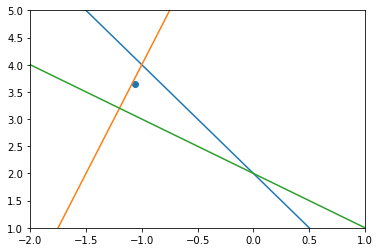
\includegraphics[width=0.7\linewidth]{figures/overdet_system}
	\caption{The three lines represent our system of equation, the point 
		the solution found with the pseudo-inverse technique.}
	\label{fig:overdet_system}
\end{figure}

Maybe you would have expected the point being at the center of gravity of the triangle, well this is not the case because the equations are not scaled the same way.


%To me the important property of the pseudo-inverse arises in solving a
%simple linear system of equations. It has 0, 1, or infinitely many
%solutions. \(𝑥=[𝐴]^+𝑏\) is the closest solution when none exists in the
%sense above. It gives the single answer when 1 exists. And when many
%exists, it is the smallest solution in the sense that \(||𝑥||_2\) is
%smallest.

\section{Principal Components Analysis}
\label{sec:pca}

Principal Component Analysis, or PCA, is a dimensionality-reduction method that is often used to reduce the complexity of large datasets, by transforming the original set of variables into a smaller one that still contains most of the initial information.

Reducing the number of variables of a dataset naturally comes at the expense of accuracy. Since smaller datasets are easier to explore and visualize, and make analyzing data simpler and faster without extraneous variables to process, the trick is to trade less accuracy for more simplicity

Let's see how this kind of technique can be implemented starting from 
a multidimensional initial dataset 
\begin{equation}
X=\begin{bmatrix}
x^{(1)}_1 &x^{(2)}_1&\cdots &x^{(m)}_1 \\
x^{(1)}_2 &x^{(2)}_2&\cdots &x^{(m)}_2 \\
\vdots &\vdots &\vdots &\vdots \\
x^{(1)}_n &x^{(2)}_n&\cdots &x^{(m)}_n 
\end{bmatrix}
\end{equation}

To allow an easier representation in the examples of this Section we will use the following two-dimensional dataset.

\begin{ipython}
import numpy as np
from matplotlib import pyplot as plt
	
np.random.seed(123)
x = 5*np.random.rand(100)
y = 2*x + 1 + np.random.rand(100)

y = np.hstack([x, y])
\end{ipython}

Left plot of Fig.~\ref{fig:pca_dataset} shows the dataset.

\subsection{Standardization}
The first step to implement PCA is to standardize the range of the variables so that each one of them contributes equally.

More specifically, the reason why it is critical to perform \emph{standardization} prior to PCA, is that the latter is sensitive to the variances of the initial variables. That is, if there are large differences between the ranges of the variables, those with larger ranges will dominate over those with small ranges (e.g. a variable that goes from 0 and 100 will dominate over another one that ranges between 0 and 1), which will lead to biased results. 

Mathematically, this can be done by subtracting the mean and dividing by the standard deviation for each component of each variable

\begin{equation}
z = \cfrac{x - \textrm{mean}}{\textrm{std dev.}}
\end{equation}

Once the standardization is done, all the variables will be transformed to the same scale.

\begin{ipython}
def centerData(X):
    X = X.copy()
    X = (X - np.mean(X, axis=0))/np.std(X, axis=0)
    return X
    
X_centered = centerData(X)
\end{ipython}

Right plot of Fig.~\ref{fig:pca_dataset} shows the standardized dataset used in the following.

Left plot of Fig.~\ref{fig:pca_dataset} shows the dataset.
\begin{figure}[htb]
	\centering
	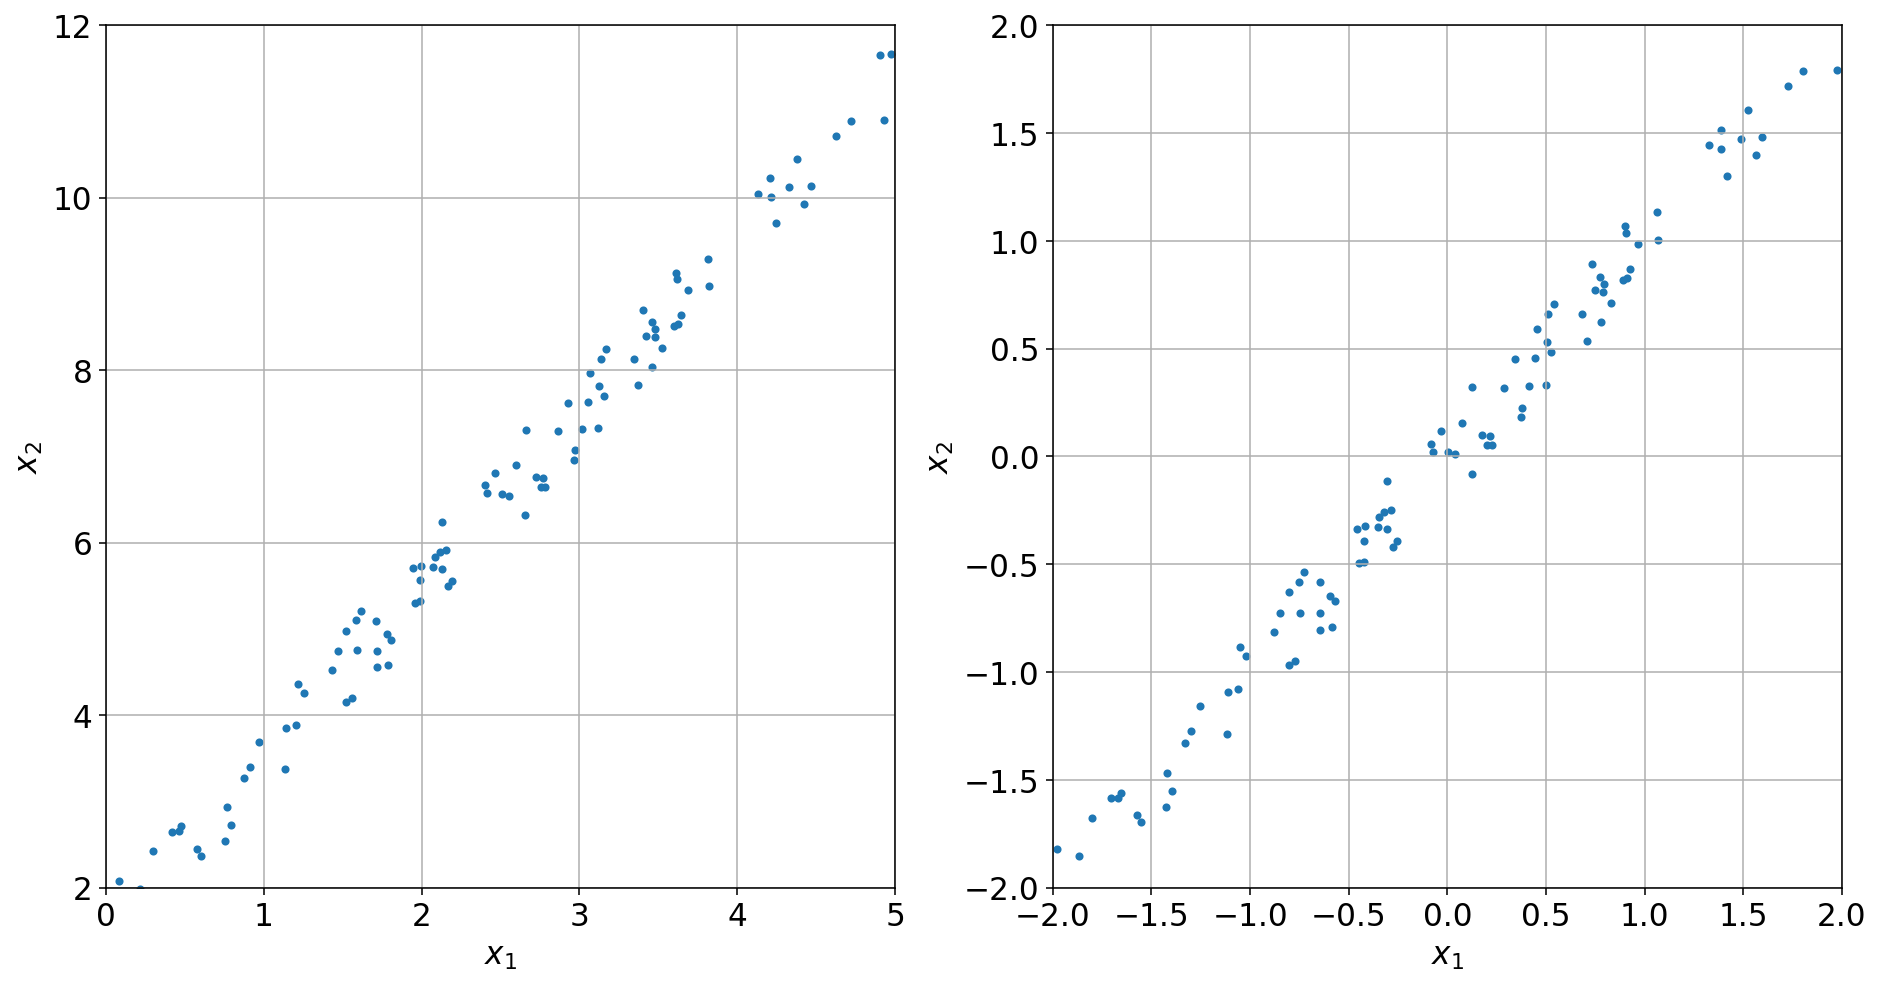
\includegraphics[width=0.9\linewidth]{figures/pca_dataset_both}
	%\includegraphics[width=0.45\linewidth]{figures/pca_dataset_centered}
	\caption{The dataset used in the PCA example (left), and the same dataset centered in the origin (right).}
	\label{fig:pca_dataset}
\end{figure}

\subsection{Covariance Matrix Computation}
The covariance matrix of our dataset helps us to understand if there is any relationship between the variables (i.e. sometimes, they are so correlated that they contain redundant information). So, in order to identify these correlations, we compute the covariance matrix.

The covariance matrix is a $n\times n$ (where $n$ is the number of dimensions) that has as entries the covariances associated with all possible pairs of the initial variables. Since the covariance of a variable with itself is its variance ($\textrm{cov}(a, a)= \textrm{var}(a)$), in the main diagonal (top-left to bottom-right) we actually have the variances of each initial variable. And since the covariance is commutative ($\textrm{cov}(a, b) = \textrm{cov}(b, a)$), the entries of the covariance matrix are symmetric with respect to diagonal.

Once we have centered our data around 0, $[X^T][X]$ is the covariance matrix.

\begin{equation}
[\Sigma]=[X^T][X] =
\begin{bmatrix}
\textrm{var}(x_1) & \textrm{cov}(x_2, x_1) & \cdots & \textrm{cov}(x_n, x_1) \\
\textrm{cov}(x_1, x_2) & \textrm{var}(x_2) & \cdots & \textrm{cov}(x_n, x_2) \\
\vdots & \vdots & \vdots & \vdots \\
\textrm{cov}(x_1, x_n) & \textrm{cov}(x_2, x_n) & \cdots & \textrm{var}(x_n)
\end{bmatrix}
\end{equation}

\subsection{Principal Components}

Principal components are new variables that are constructed as linear combinations or mixtures of the initial variables. These combinations are done in such a way that the new variables (i.e. principal components) are uncorrelated and most of the information within the initial variables is squeezed or compressed into the first components. 

So, the idea is that a $n$-dimensional dataset gives you $n$ principal components, but PCA tries to put maximum possible information in the first component, then maximum remaining information in the second and so on.

Organizing information in principal components this way, will allow you to reduce dimensionality without losing much information, and this by discarding the components with low information and considering the remaining components as your new variables.
%An important thing to realize here is that, the principal components are less interpretable and don’t have any real meaning since they are constructed as linear combinations of the initial variables.

Geometrically speaking, principal components represent the directions of the data that explain a maximal amount of variance, that is to say, the lines that capture most information of the data. The relationship between variance and information here, is that, the larger the variance carried by a line, the larger the dispersion of the data points along it, and the larger the dispersion along a line, the more the information it has.

It is possible to demonstrate that the eigenvectors of the covariance matrix are actually the directions of the axis where there is the most variance (i.e. most information) and that we call \emph{principal components}. Eigenvalues are simply the coefficients, attached to eigenvectors, which give the amount of variance carried in each principal component.

As we have seen in Sec.~\ref{find-eigenvalues-and-eigenvectors-in-python} the eigenvectors and eigenvalues of our dataset covariance are obtained as follows

\begin{ipython}
eigVals, eigVecs = np.linalg.eig(X_centered.T.dot(X_centered))
print (eigVecs)
\end{ipython}
\begin{ioutput}
[[-0.70710678 -0.70710678]
 [ 0.70710678 -0.70710678]]
\end{ioutput}

\begin{ipython}
print (eigVals)
\end{ipython}
\begin{ioutput}
[  7.46600865 192.53399135]
\end{ioutput}

If we rank the eigenvalues in descending order, we get $\lambda_2>\lambda_1$, which means that the eigenvector that corresponds to the first principal component (PC1) is  $v_2$ (i.e. the second column of the previous matrix).

After having the principal components, to compute the percentage of variance (information) accounted for by each component, we divide the eigenvalue of each component by the sum of eigenvalues. 

\begin{ipython}
for l in eigVals:
    print (f"{l/np.sum(eigVals)*100:.1f}")
\end{ipython}
\begin{ioutput}
3.7
96.3
\end{ioutput}

According to these results PC2 and PC1 carry respectively 96\% and 4\% of the variance of the data.

\subsection{Feature Vector}
Given the list of eigenvectors and eigenvalues we need to choose whether to keep all these components or discard those of lesser significance (i.e. of low eigenvalues), and form with the remaining ones a matrix called \emph{feature vector}.

So, the feature vector is simply a matrix that has as columns the eigenvectors of the components that we decide to keep. This makes it the first step towards dimensionality reduction, because if we choose to keep only $p$ eigenvectors (components) out of $n$, the final dataset will have only $p$ dimensions.

Continuing with the example from the previous step, we can either form a feature vector with both of the eigenvectors $v1$ and $v2$, or discard the eigenvector $v_2$, which is the one of lesser significance, and form a feature vector with $v_1$ only.

Discarding the eigenvector $v_1$ will reduce dimensionality by 1, and will consequently cause a loss of information in the final data set. But given that $v_1$ was carrying only 4\% of the information, the loss will be therefore not important and we will still have 96\% of the information that is carried by $v_2$.

Figure~\ref{fig:pca_result} shows the two principal components.

\begin{figure}[htb]
	\centering
	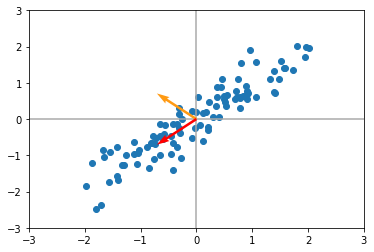
\includegraphics[width=0.7\linewidth]{figures/pca_result}
	\caption{The directions corresponding to the first two principal 
		components of our example dataset.}
	\label{fig:pca_result}
\end{figure}

\subsection{Recast Data Along Principal Components}
At this point we can use the feature vector to reorient data from the original axis to the ones represented by the principal components. 
This can be done by multiplying the transpose of the original dataset by the transpose of the feature vector

\begin{equation}
[Y] = [X^T][F^T]
\end{equation}

\begin{ipython}
Y = eigVecs.T.dot(X_centered.T)
\end{ipython}

The rotation transformed our dataset that have now the more variance on one of the basis axis (i.e. the Cartesian axis). 
You could keep only this dimension and have a fairly good representation of the data. Figure~\ref{fig:pca_rotated} shows the effect of such a rotation to our sample.
\clearpage
\begin{figure}[htb]
	\centering
	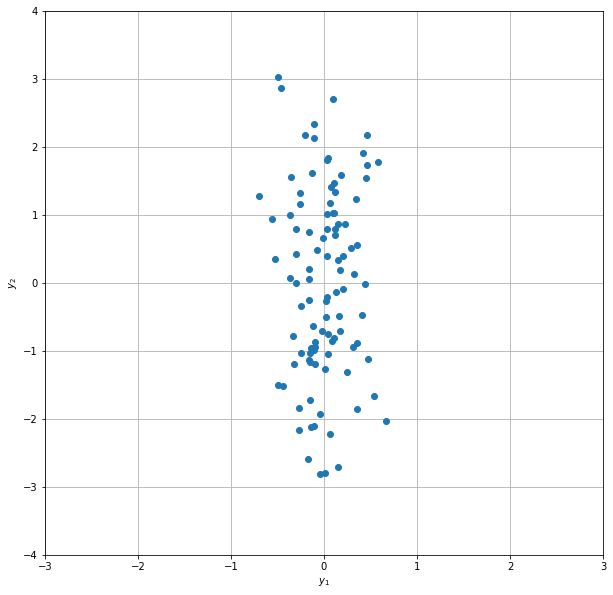
\includegraphics[width=0.5\linewidth]{figures/pca_rotated}
	\caption{The dataset rotated so that the usual Cartesian coordinates
		correspond to the first two principal components.}
	\label{fig:pca_rotated}
\end{figure}

\subsection{Impact of Covid19}
Using PCA analysis it can be assessed the impact of the Covid19 pandemic on different stocks, clustering together assets that were most/least affected without any prior knowledge of their fundamental.

In this analysis we are going to use the equities forming the \emph{Dow Jones 30} index, so the first step is to download their returns with \texttt{yfinance} package (the data availability is from March 2019 to today).

\begin{ipython}
import yfinance as yf

tickers = ["BA","CAT","CVX","CSCO","KO",
	       "DOW","XOM","GS","HD","INTC","IBM",
	       "JNJ","JPM","MCD","MRK","MSFT","NKE",
	       "PFE","PG","RTX","TRV","UNH","VZ",
	       "V","WBA", "WMT", "^DJI"]
	
proxy = yf.Tickers(tickers)           
df = proxy.history(start='2020-01-02',
                   end='2020-08-16')['Close'].pct_change().dropna()
\end{ipython}

After downloading data the PCA analysis is performed
\begin{ipython}
import numpy as np
	
equities = df.iloc[:, :-1]
cov = equities.cov()
eigVals, eigVecs = np.linalg.eig(cov)
\end{ipython}

Let's look at the first principal component and select the corresponding stocks that have the best and the worst PCA weights, as shown in Fig.~\ref{fig:pca_covid_neg}.

\begin{figure}[htb]
\centering
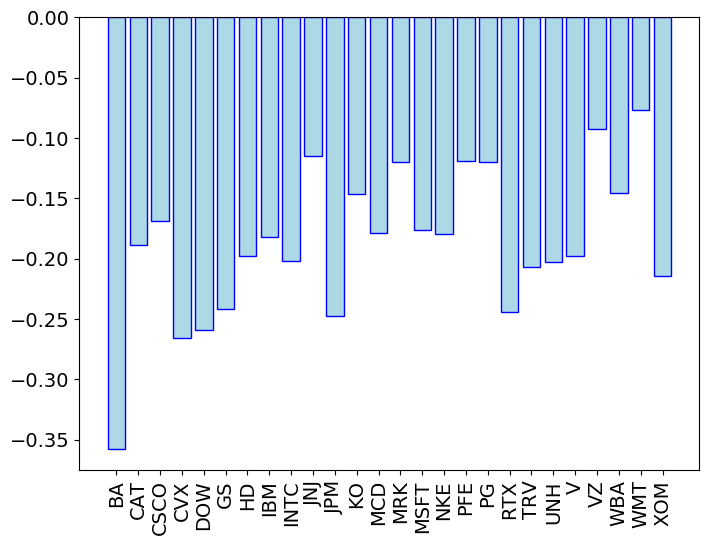
\includegraphics[width=.6\textwidth]{figures/pc1_weights_covid}
\caption{Ten most negative (top) and least negative (bottom) weights of the PC1 portfolio.}
\label{fig:pca_covid_neg}
\end{figure}

Notice from Figure~\ref{fig:pca_covid_neg} how the most negative stocks are Boing and Chevron, connected to travel and energy sector. This makes sense since Covid19 heavily impacted the traveling business, as well as the energy companies that provide fuels for those business. On the other hand, the least impacted companies are Verizon, Wallmart, Pfizer and Johnson \& Johnson, which belong to sectors boosted during the quarantine measures and the pandemic in general.

In addition we can check the winning portfolio that is long the top 3 companies according to the PCA weights.

\begin{ipython}
# normalize weights
norm_eigVecs = abs(eigVecs.T[0])/sum(abs(eigVecs.T[0]))
	
# market portfolio
pc_daily_ret = equities.dot(norm_eigVecs)
pc_cum_ret = pc_daily_ret.cumsum()
	
# worst portfolio
worst_idx = np.argsort(eigVecs.T[0])[:3]
eq_worst = equities.iloc[:, worst_idx]
worst_eigv = norm_eigVecs[worst_idx]
worst_ret = eq_worst.dot(worst_eigv).cumsum()
print ("Worst :", df.columns[worst_idx])
	
# best portfolio         
best_idx = np.argsort(eigVecs.T[0])[-3:]
eq_best = equities.iloc[:, best_idx]
best_eigv = norm_eigVecs[best_idx]
best_ret = eq_best.dot(best_eigv).cumsum()
print ("Best :", df.columns[best_idx])
\end{ipython}
\begin{ioutput}
Worst : Index(['BA', 'CVX', 'DOW'], dtype='object')
Best : Index(['JNJ', 'VZ', 'WMT'], dtype='object')
\end{ioutput}

As shown in Figure~\ref{fig:pca_covid_return}, the resulting portfolio would have performed significantly better than the market, since it invested in companies that actually didn't suffer to much from the pandemic. 

\begin{figure}[bhtp]
\centering
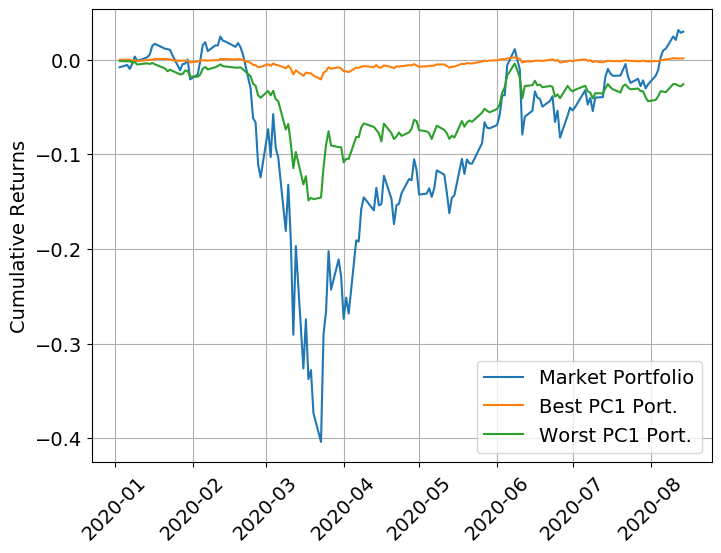
\includegraphics[width=.7\textwidth]{figures/pc1_weights_covid_returns}
\caption{Three most negative and least negative weights portfolios compared to the market portfolio.}
\label{fig:pca_covid_return}
\end{figure}

Note that this portfolio is formed with look-ahead bias, indeed portfolio weights are computed using future dates that were not available at the time of market downturn. The PCA used in this way is therefore a backward looking analytics tool.
































\subsection{Dimension Reduction}
In statistics, dimensionality reduction is the transformation of data such that the number of variables is reduced by obtaining principal variables. Dimensionality reduction can help us see the key structure of original data. For example, if the data lies in a low dimensional subspace, it is conceivable that one could restrict our learning problem to this low dimensional subspace and thereby simplify it.

There are two techniques of dimensionality reduction that can be applied to the feature
space:
\begin{itemize}
\item feature selection: is the process of selection of a subset of relevant features, which can be done manually based on domain knowledge or using statistical tools
\item feature projection: converts data from high-dimensional space to low-dimensional space. The data transformation can be linear or nonlinear.
\end{itemize}

The basic linear technique for dimensionality reduction, the principal component analysis (PCA), performs a linear mapping of the data into a smaller space such that the variance of the data in the low-dimensional representation is maximized. 

In practice, a covariance matrix (and sometimes a correlation matrix) of the data is constructed, and the eigenvectors of this matrix are calculated. The eigenvectors corresponding to the largest eigenvalues (principal components) can now be used to recover most of the variance of the original data. Moreover, the first few eigenvectors can often be interpreted in terms of the large-scale physical behaviour of the system. 

The original space (with a dimension equal to the number of points) is reduced (with loss of data, but with the hope that the most important variance remains) to a space stretched over a few eigenvectors.

\subsection{Principal Component Analysis}
The goal of PCA is to find an alternative representation of data $X$ in the transformed space so that $X$ can be approximated by variables of smaller dimensions while maintaining a given level of the original information.
Let us denote a zero mean $p$-dimensional feature space $X = (X_1, \ldots, X_p)$. We aim to obtain a \textbf{linear} transformation $V$ such that the $p$-dimensional transformed feature variable $Z := XV$ consists of components orthogonal to each other, and the variances of those components are in descending order. Alternatively, we are aiming to find the representation of $\tilde{X} = ZV^{-1}$ can be seen as a projection onto a new feature space, on which a dimensionality reduction approach can be built.

Figure~\ref{fig:pca_dataset} illustrates the main idea of PCA: to find such orthogonal vectors (principal components) $Z_k$ for $k = 1,\ldots, p$, and to reduce the dimensionality of the original data $X$ by mapping this data to the space generated by first $l$, $l = 1,\ldots, p - 1$ vectors. % (on this figure $p = 3$ and $l = 2$).

%Right plot of Fig.~\ref{fig:pca_dataset} shows the standardized dataset used in the following.

Left plot of Fig. shows the dataset.
\begin{figure}[htb]
	\centering
	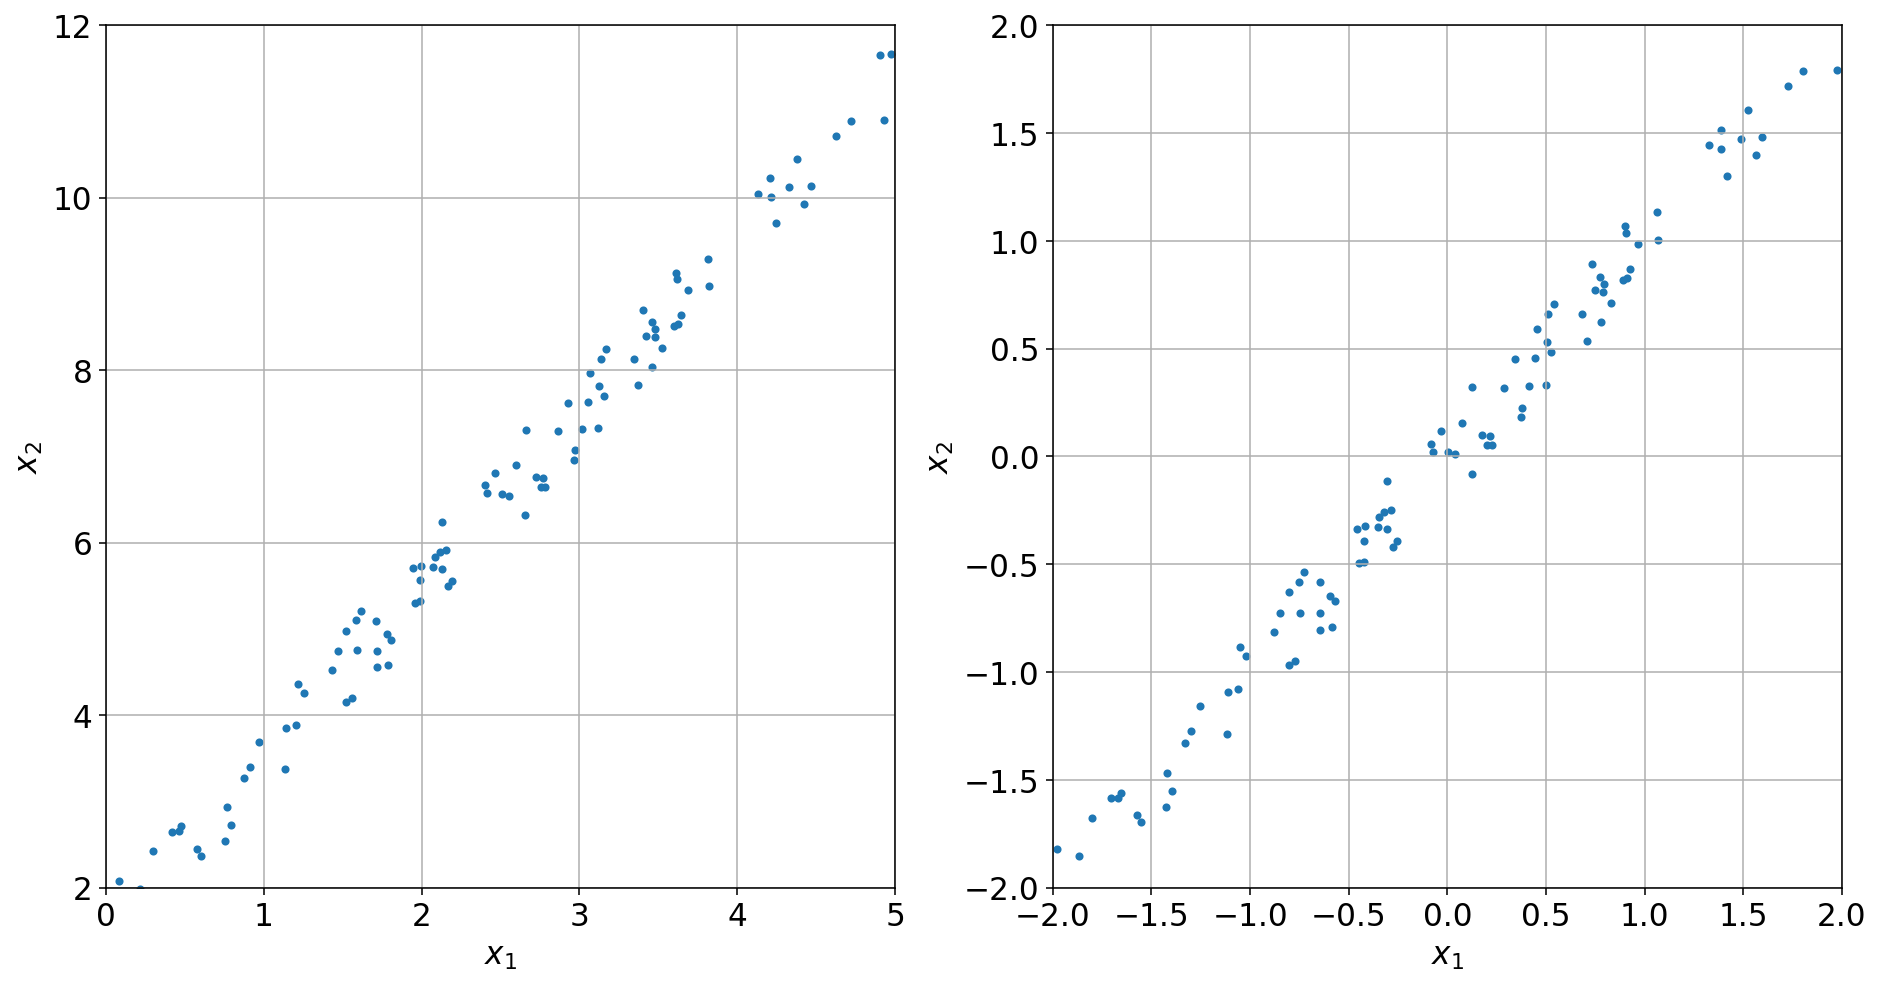
\includegraphics[width=0.9\linewidth]{figures/pca_dataset_both}
	%\includegraphics[width=0.45\linewidth]{figures/pca_dataset_centered}
	\caption{The dataset used in the PCA example (left), and the same dataset centered in the origin (right).}
	\label{fig:pca_dataset}
\end{figure}


\subsection{Principal components and covariance}
Let’s recall some basic definitions from probability theory and statistics:
\begin{itemize}
\item for the vector $X = (X_1, X_2, \ldots, X_k)$ of $k$ jointly distributed random variables with finite second moments, its auto-covariance matrix $\SigmaX$ is defined as follows:
\begin{equation}
\Sigma_X = \text{Cov}(X, X) = E[(X − E[X])(X − E[X])^T] = E[XX^T]–E[X]E[X]^T
\end{equation}
\item let $X$ be a random vector with covariance matrix $\Sigma_X$, and let $A$ be a matrix that can
act on $X$ on the left. The covariance matrix of the matrix-vector product $AX$ is:
\begin{equation}
\text{Cov}(AX, AX) = E[(AX)(AX)^T]–E[AX]E[(AX)^T] = E[AXX^T A^T]–E[AX]E[A^T X^T] = AE[XX^T]A^T − AE[X]E^T A^T =
= A(E[XX^T]–E[X]E[X]^T)A^T = A\Sigma_XA^T
\end{equation}
\item The empirical covariance matrix $X$ can be written as 
\begin{equation}
\Sigma_X = \cfrac{1}{N − 1}XX^T
\end{equation}
\item For every $n\times n$ real symmetric matrix, the eigenvalues are real and the eigenvectors can be chosen real and orthonormal. Thus a real symmetric matrix $A$ can be decomposed as
\begin{equation}
A = Q\Lambda Q^T
\end{equation}
where $Q$ is an orthogonal matrix whose columns are (the above chosen, real and orthonormal) eigenvectors of $A$, and $\Lambda$ is a diagonal matrix whose entries are the eigenvalues of $A$.
By using the \emph{singular value decomposition} we can write this empirical matrix:
\begin{equation}
\Sigma_X = \cfrac{1}{N-1}XX^T = \cfrac{1}{N-1}(UDV^T)(UDV^T)^T = V\left(\cfrac{1}{N-1}D^2\right) V^T
\end{equation}

Additionaly as the covariance matrix $\Sigma_X$ is a real non-negative symmetric matrix we can use an \emph{eigenvalue decomposition}:
\begin{equation}
\Sigma_X = Q\Lambda Q^T
\end{equation}

It is clear that the right singular vectors in equation ... are the eigenvectors in ...p: $V = Q$, and the diagonal matrix $\Lambda = \text{diag}(\lambda_1, \ldots, \lambda_p)$ is $\left(\frac{1}{N-1}D^2\right)$, i.e componentwise:
\begin{equation}
\lambda_j = \cfrac{d_j}{N − 1}
\end{equation}

That means that the new coordinates $V$ are given by the eigenvectors of the covariance matrix.
Now finally the empirical covariance matrix of the principal components $Z$ can be rewritten
\begin{equation}
\Sigma_Z = \cfrac{1}{N-1}Z^T Z = \cfrac{1}{N-1}(XV)^T(XV)=V^T\Sigma_X V = \cfrac{D^2}{N-1} = \Lambda
\end{equation}
\end{itemize}

To summarize:
\begin{enumerate}
\item The principal components $Z_1, \ldots, Z_p$ are orthogonal (i.e. $Z^{-1}=Z^T$), and the variances of $Z_1,\ldots, Z_p$ are the eigenvalues of the covariance matrix of $X$ in descending order.
\item With the representation of the covariance of the data using SVD, we can apply PCA to reduce the dimensionality of the data.

Once we have the principal components and the loading matrix, the representation of $X$ becomes
\begin{equation}
X = ZV^{−1} = ZV^T = \sum_{j=1}^{p}Z_j v_j^T
\end{equation}

Thus an approximating sequence of feature variables $X$ is obtained. In section (2.5) we have shown that $\hat{X˜}(k)$ including the first $k$ principal components of $X$:
\begin{equation}
\hat{X}^{(k)} = \sum_{j=1}^{k}Z_j v_j^T
\end{equation}
covers such proportion
\begin{equation}
\cfrac{\sum_j=1}^k \lambda_j}{\sum_j=1}^p \lambda_j}
\end{equation}
of the variance of $X$. From the equation above, it is obvious that if we take $k = p$, we recover all the original data of $X$.

Assuming, therefore, that the information is incorporated in the covariance, given the data set $X$ and the information preservation criterion in the form of the percentage of variance explained, we can find an approximation of $X$ with reduced dimensionality.
The residual from the approximation using $k$ PCs is 
\begin{equation}
R^{(k)} = X − \tilde{X}˜^{(k)} = \sum_{j=k+1}^{p}Z_j v^T_j
\end{equation}

\subsection{Practical problems}
PCA is not invariant to scaling. Before applying PCA, we should consider whether or not to standardize the data $X$, besides removing of the mean from the data before applying PCA. In practice, it depends on the context of the data and the objective, but there are two general tips regarding this problem:
\begin{enumerate}
\item If features are measured in different units that are not comparable, we should first standardize them before applying PCA.
\item If features are measured in comparable units, then we can keep them unscaled to preserve the original variability information.
\end{enumerate}

Furthermore PCA can not be used if the data is not Gaussian. PCA is based on the assumption that the data is normally distributed, that is why we can represent all the information from the covariance. In the case of non-Gaussian data, independent component analysis (ICA) is often used.



















\section*{Exercises}
\cprotEnv\begin{question}
Write a program to compute the multiplication of following matrices

\begin{equation*}
[P] = \begin{bmatrix}
1& 0\\
0& 1
\end{bmatrix};\quad
[Q] = \begin{bmatrix}
	1& 2\\
	3& 4
\end{bmatrix}
\end{equation*}
\end{question}

\cprotEnv\begin{solution}
\begin{ipython}
import numpy as np
p = [[1, 0], [0, 1]]
q = [[1, 2], [3, 4]]
print("original matrix:")
print(p)
print(q)

result1 = np.dot(p, q)
print("Result of the said matrix multiplication:")
print(result1)
print(result2)
\end{ipython}
\begin{ioutput}
original matrix:
[[1, 0], [0, 1]]
[[1, 2], [3, 4]]
Result of the said matrix multiplication:
[[1 2]
 [3 4]]
\end{ioutput}
\end{solution}

\cprotEnv\begin{question}
Write a program to compute the eigenvalues and eigenvectors of a given square array

\begin{equation*}
	[M] = \begin{bmatrix}
		3& -2\\
		1& 0
	\end{bmatrix}
\end{equation*}
\end{question}

\cprotEnv\begin{solution}
\begin{ipython}
import numpy as np

m = np.array([[3, -2],[1, 0]])
print("Original matrix:")
print(m)

w, v = np.linalg.eig(m) 
print("Eigenvalues of the said matrix", w)
print("Eigenvectors of the said matrix", v)
\end{ipython}
\begin{ioutput}

Original matrix:
[[ 3 -2]
 [ 1  0]]
Eigenvalues of the said matrix [ 2.  1.]
Eigenvectors of the said matrix [[ 0.89442719  0.70710678]
                                 [ 0.4472136   0.70710678]]
\end{ioutput}
\end{solution}

\cprotEnv\begin{question}
Write a program to compute the inverse of a given matrix

\begin{equation*}
	[M] = \begin{bmatrix}
		1& 2\\
		3& 4
	\end{bmatrix}
\end{equation*}
\end{question}

\cprotEnv\begin{solution}
\begin{ipython}
import numpy as np

m = np.array([[1,2],[3,4]])

print("Original matrix:")
print(m)

result =  np.linalg.inv(m)
print("Inverse of the said matrix:")
print(result)
\end{ipython}
\begin{ioutput}

Original matrix:
[[1 2]
 [3 4]]
Inverse of the said matrix:
[[-2.   1. ]
 [ 1.5 -0.5]]
\end{ioutput}
\end{solution}

\cprotEnv\begin{question}
A \emph{vampire number} is a composite number with an even number of digits, that can be factored into two natural numbers each with half as many digits as the original number, where the two factors (called \emph{fangs}) contain precisely all the digits of the original number (in any order). The first vampire number is $1260 = 21 \times 60$.

Similarly a \emph{vampire matrix} is a matrix such that squaring it, the resulting matrix elements are vampire numbers. An example is:
\begin{equation*}
\begin{bmatrix}
23 & 76 \\
69 & 78 \\
\end{bmatrix}^{2} =
\begin{bmatrix}
2323 & 7676 \\
6969 & 7878 \\
\end{bmatrix}
\end{equation*}

A ($2\times 2$) vampire matrix with three digits elements $[M]$ must satisfy the following conditions
\begin{equation*}
[M]^2 = 1001 [M]
\end{equation*}
\noindent
Implement an algorithm to find the first three $2\times 2$ vampire matrices with three digits elements (i.e. the elements to try must be in $[100,999]$ range). 
\end{question}
\cprotEnv\begin{solution}
\begin{ipython}
import numpy as np

successes = 0
factor = 1001

for i1 in range(100, 1000):
    for i2 in range(100, 1000):
        for i3 in range(100, 1000):
            for i4 in range(100, 1000):
                M = np.array([[i1, i2], [i3, i4]])
                M2 = np.dot(M, M)
                if np.array_equal(M2, factor*M):
                    successes += 1
                    print (M)
                    print (M2)
                    print ()
                    if successes == 3:
                        import sys
                        sys.exit()
\end{ipython}
\begin{ioutput}
[[100 100]
 [901 901]]
[[100100 100100]
 [901901 901901]]

[[100 106]
 [850 901]]
[[100100 106106]
 [850850 901901]]

[[100 170]
 [530 901]]
[[100100 170170]
 [530530 901901]]
\end{ioutput}
\end{solution}

\cprotEnv\begin{question}
Write a \texttt{numpy} program to get the lower-triangular $[L]$ in the Cholesky decomposition of the following array

\begin{equation*}
	[A] = \begin{bmatrix}
		4& 12 & -16\\
		12& 37 & -53\\
		-16& -53 & 98
	\end{bmatrix}
\end{equation*}
\end{question}

\cprotEnv\begin{solution}
\begin{ipython}
import numpy as np

a = np.array([[4, 12, -16], [12, 37, -53], [-16, -53, 98]])

print("Original array:")
print(a)

L = np.linalg.cholesky(a)
print("Lower-triangular L in the Cholesky decomposition of the said array:")
print(L)
\end{ipython}
\begin{ioutput}
Original array:
[[  4  12 -16]
 [ 12  37 -53]
 [-16 -53  98]]
Lower-triangular L in the Cholesky decomposition of the said array:
[[ 2.  0.  0.]
 [ 6.  1.  0.]
 [-8. -5.  3.]]
\end{ioutput}
\end{solution}

\begin{thebibliography}{9}
\bibitem{bib:matrices}\href{https://algebra.nipissingu.ca/tutorials/matrices.html}{\emph{Matrices Tutorial}}, Nipissing University [Online]
\bibitem{bib:eigenvalues}\href{http://macosa.dima.unige.it/mat/calculus/eigenstuff.htm}{\emph{Eigenvectors and Eigenvalues}}, UniGe [Online]
\bibitem{bib:pca} L. I. Smith, \href{http://www.iro.umontreal.ca/~pift6080/H09/documents/papers/pca_tutorial.pdf}{\emph{A tutorial on Principal Component Analysis}} [Online]
\end{thebibliography}






  % da riguardare
\chapter{Random Variables}
\label{fundamentals}

In this Chapter some basic concepts that will be used throughout the remaining part of these notes, are reviewed.

\section{Random Variable}
\label{random-variables}

In probability and statistics a \emph{random variable} is described as a variable whose values depend on outcomes of a random phenomenon. 

The word "variable" in random variable is a misnomer since it is actually a function. And like all well behaved functions, a random variable, say $X$, has a domain and a range.
The domain $\Omega$ of $X$ is the sample space of random outcomes. These outcomes arise when some stochastic experiment is performed. As a function, a random variable is required to be measurable, \emph{which allows for probabilities to be assigned to its potential values.} 

In the corporate world, random variables can be assigned to properties such as the average price of an asset over a given time period or the return on investment after a specified number of years. Risk analysts assign use random variables to model the probability of an adverse event occurring. 

A random variable is different from an algebraic one. The former has a set of possible values, and any of those values could be the resulting outcome. The latter is an unknown value that can be calculated (e.g. $x$ in equation $10 + x = 13$ can be solved to get $x=3$).

When the range of possible values for $X$ is infinite then $X$ is called a \emph{continuous random variable}. Contrary if the range is countable, the random variable is called a \emph{discrete random variable}. In both cases its distribution can be interpreted as a \emph{probability density function} (PDF), see Fig.~\ref{fig:pdf_pmf}.
Since by definition the PDF is non-negative everywhere, and its integral over the entire space is equal to 1 it represent the likelihoods of occurrences of events in the sample space. 

\begin{figure}[htb]
	\centering
	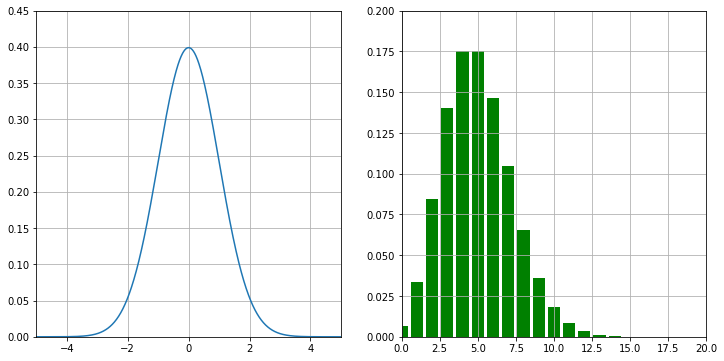
\includegraphics[width=1.\textwidth]{figures/pdf_pmf.png}
	\caption{On the left an example of continuous probability density function (Normal), on the right a discrete probability mass function (Poissonian).}
	\label{fig:pdf_pmf}
\end{figure}

\subsection{Cumulative Distribution and Quantile Functions}
\label{sec:quantile-function}

The \emph{cumulative distribution function} (CDF) $F$ of a random variable $X$, evaluated at $x$, gives the probability that $X$ will take a value less than or equal to $x$

\begin{equation}
F_X(x) = P(X \le x)\qquad\mathrm{or~equivalently}~\int_{-\infty}^{x}{f(X)dX}
\end{equation}
so it gives the area under the probability density function $f$ from minus infinity to $x$.
The probability that $X$ lies in the interval $(a,b]$ is therefore

\begin{equation}
P(a> X \le b)=F_{X}(b)-F_{X}(a)\qquad\mathrm{or}~\int_a^b{f(X)dX}
\end{equation}
Notice that by the previous definition any random variable can be conveniently described by its cumulative distribution too.

The \emph{quantile function} $Q$, associated with a probability distribution of a random variable, specifies the value $x$ of the random variable such that the probability $p$ of the variable being less than or equal to that value equals the given probability. It is also called the percent-point function (PPF) or inverse cumulative distribution.

In terms of the cumulative distribution function $F$, the quantile function $Q$ returns the value $x_p$ such that 

\begin{equation}
F_{X}(x_p)=P(X\le x_p)=p
\end{equation}
So the quantile function can be considered the "inverse" of the cumulative distribution function: given a probability $p$ it returns the $x$ such that the CDF $F_X(x) = p$, so we can write $Q=F^{-1}(p)$, see Fig.~\ref{fig:percentile}. 

\begin{figure}[htb]
	\centering
	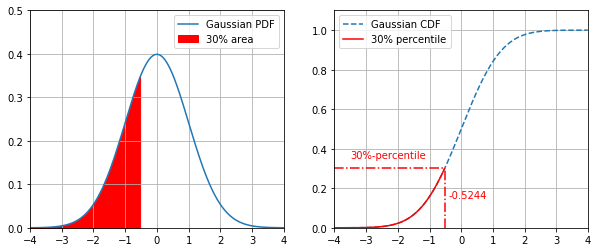
\includegraphics[width=1.\textwidth]{figures/percentile.png}
	\caption{On the left side the Gaussian PDF is drawn, the red area represents the 30\% of the total area. On the right the corresponding CDF is plotted, the point at which the CDF reaches 30\% is highlighted. The corresponding quantile value is also indicated and is $-0.5244$.}
	\label{fig:percentile}
\end{figure}

The computation of CDF and quantiles is quite simple in \texttt{python}. The implementation of many distributions is available in the \texttt{scipy.stats} module and for each of them the methods \texttt{cdf(x)} and \texttt{ppf(x)} can be used to evaluate CDF and quantile respectively.

\pythoncodenon{code/random_variables_1.py}

\begin{ioutput}
30%-quantile of standard normal is -0.5244
CDF value at -0.5244: 0.3000
\end{ioutput}

Similar calculations can be carried on a dataset (e.g. \texttt{numpy.array}) using the function \texttt{numpy.percentile} (e.g. this will be useful when estimating VaR). Notice that in this case we are talking about \emph{percentile} which is the \emph{quantile} times 100 (e.g. 50-percentile is equivalent to 0.5-quantile).

\pythoncodenon{code/random_variables_2.py}

\begin{ioutput}
[1.08 5.  ]
\end{ioutput}

\subsection{Expected Value}\label{sec:expected-value}

Since a random variable is connected to probabilistic events, it is necessary to take into account all the possible values it can take for its \textit{"evaluation"}. This is done with the \emph{expected value} which is intuitively the weighted mean of all the possible realizations of the random variable $X$.

Consider a discrete random variable with a finite number of outcomes $(x_{1},x_{2},\ldots ,x_{k})$ occurring with probabilities $(p_{1},p_{2},\ldots ,p_{k})$ respectively. The expectation of $X$ is then defined as

\begin{equation}
\mathbb{E}[X]=\sum _{i=1}^{k}x_{i}\,p_{i}=x_{1}p_{1}+x_{2}p_{2}+\cdots +x_{k}p_{k}
\end{equation}
which is indeed the average of the $x_{i}$ weighted by their probabilities $p_{i}$.

As an example let $X$ represent the outcome of a single roll of a fair six-sided die. The possible values for $X$ are 1, 2, 3, 4, 5, and 6, all of which are equally likely with probability $1/6$.

The expectation of $X$ is then

\begin{equation*}
\mathbb{E}[X]=1\cdot {\frac {1}{6}}+2\cdot {\frac {1}{6}}+3\cdot {\frac {1}{6}}+4\cdot {\frac {1}{6}}+5\cdot {\frac {1}{6}}+6\cdot {\frac {1}{6}}=3.5
\end{equation*}

If instead $X$ is a random variable with a probability density function, $f(x)$, then the expected value is generalized as

\begin{equation}
\mathbb{E}[X]=\int_{\Omega}xf(x)dx
\end{equation}
%For multidimensional random variables, the expected value is defined per component, that is,
%
%\begin{equation}
%\mathbb{E}[(X_{1},\ldots ,X_{n})]=(\mathbb{E} [X_{1}],\ldots ,\mathbb{E}[X_{n}])
%\end{equation}

\subsection{Some Properties of Expected Value}
\label{some-properties}

\begin{itemize}
\tightlist
\item Let $\mathbbm{1}_{A}$ denote the indicator function of an event $A$ (i.e. a function whose value is 1 if the event $A$ happens, 0 otherwise), then

\begin{equation}
\mathbb{E}[\mathbbm{1}_{A}] = 1\cdot P(A)+0\cdot P(\Omega \setminus A)= P(A)
\end{equation}

\item the expected value operator \(\mathbb{E}\) is linear so for any random variables $X$ and $Y$, and a constant $a$
\begin{equation}
\begin{cases}
\mathbb{E}[X+Y] = \mathbb{E}[X] + \mathbb{E}[Y] \\
\mathbb{E}[aX] = a\mathbb{E}[X]
\end{cases}
\end{equation}

This means that the expected value of the sum of any finite number of random variables is the sum of the expected values of the individual random variables, and the expected value scales linearly with a multiplicative constant;

\item the expected value of a measurable function of $X$, $g(X)$, given that $X$ has a probability density function $f(x)$, is given by 

\begin{equation}
\mathbb{E}[g(X)] = \int_{\Omega}g(x)f(x) dx
\end{equation}

%This formula also holds in multidimensional case, when $g$ is a function of several random variables, and $f$ is their joint density;

\item $n$ random variables $X_1 ,\ldots , X_n$ are independent if the following property holds for all positive functions $f_1 ,\ldots , f_n$

\begin{equation}
\mathbb{E}[f_1 (X_1 )\cdots f_n (X_n )] = \mathbb{E}[f_1 ( X_1 )] \cdots \mathbb{E}[f_n (X_n )]
\end{equation}
\end{itemize}


%
%We have seen so far how to generate a sequence of random numbers from U
%{[}0, 1{]}. However, most of the simulations include the sampling of
%random variables, or even random vectors in a mul- tidimensional case,
%from specified, not uniform distributions. Sampling of nonuniform random
%variates is done indirectly, i.e.~one transforms samples from the
%uniform to a desired nonuniform distribution. Accordingly, each
%realization of a nonuniform random variable is directly obtained from a
%single uniform variate or from a sequence of uniforms {[}46, p.54{]}.
%There are numerous algorithms that allow you to generate random numbers
%from a certain desired distribution. However, two main criteria in order
%to choose between them are accuracy and speed.


%
%\hypertarget{correlated-normal-variables-and-vectors}{%
%\subsubsection{Correlated normal variables and
%	vectors}\label{correlated-normal-variables-and-vectors}}
%
%A \(d\)-variate normal distribution \(\phi(\mu, \Sigma)\) is generally
%specified by its mean vector \(\mu\) and variance- covariance matrix
%\(\Sigma\). Random vectors from a multivariate normal distribution can
%be generated directly by generating a \(d\)-vector of iid standard
%normal deviates \(z' = (z_1 , z_2 ,\dots , z_d)\).
%
%Next we know from the linear transformation property that if the vector
%\(z∼\phi_d (0,I)\) and \(x = \mu + Az\), then \(x ∼\phi_d (\mu, AA')\).
%Therefore, we can generate a sequence of univariate normal random
%variables \(z_i\) and put them into a vector \(z\). Thus the challenge
%is merely made up of finding the matrix \(A\) for which the property
%\(AA' = \Sigma\) holds. The representation of \(\Sigma\) as \(AA'\) with
%\(A\) as a lower triangular matrix is denoted as a Cholesky
%factorization of the variance-covariance matrix \(\Sigma\). If
%\(\Sigma\) is symmetric positive definite there is a Cholesky
%factorization and the sampling of multivariate normals is easily done by
%basically sampling from a univariate \(\phi(0,1)\).
%
%In some applications in finance random variables or vectors are required
%to depend on each other in a prescribed way, i.e.~they must not be
%totally uncorrelated. Correlated random variables are calculated
%according to the following algorithm:
%
%\begin{enumerate}
%\def\labelenumi{\arabic{enumi}.}
%\tightlist
%\item
%calculate the Cholesky factorization \(AA′ = \Sigma\),
%\item
%calculate \(z ∼ \phi(0,I)\) by component, for \(i = 1,2,\ldots ,d\),
%\item
%\(x=\mu + Az\), then \(x∼\phi (\mu, \Sigma )\).
%\end{enumerate}
%
%Suppose we have a two-dimensional case, \(d = 2\). Next we are looking
%for a vector \(x' = (x_1 , x_2 ) ∼ \phi (0, \Sigma )\). The correlation
%between \(x_1\) and \(x_2\) is denoted by \(\rho\) and thus the Cholesky
%factorization provides \(\Sigma = AA'\)
%
%\[\begin{bmatrix}
%\sigma_1^2 & \rho\sigma_1 \sigma_2\\
%\rho\sigma_1 \sigma_2 & \sigma_2^2 
%\end{bmatrix} = 
%\begin{bmatrix}
%\sigma_1 & 0\\
%\rho\sigma_2 & \sigma_2\sqrt{1-\rho^2} 
%\end{bmatrix}
%\begin{bmatrix}
%\sigma_1 & \rho\sigma_2 \\
%0 & \sigma_2\sqrt{1-\rho^2} 
%\end{bmatrix}\]
%
%If \(z_1\) and \(z_2\) are independent and from \(\phi(0, 1)\), then
%
%\[\begin{bmatrix}
%x_1\\
%x_2 
%\end{bmatrix} = A
%\begin{bmatrix}
%z_1\\
%z_2 
%\end{bmatrix} = 
%\begin{bmatrix}
%\sigma_1 z_1\\
%\sigma_2 (\rho z_1 + \sqrt{1-\rho^2}z_2) 
%\end{bmatrix}
%\]
%
%are distributed according to \(\phi(0, \Sigma)\).


\section*{Exercises}
\begin{question}
A random variable $X$ that assumes values in the interval $[0, 1]$ has density function $f(x) = a + b x$,
where $a$ and $b$ are two constants to be determined.

\begin{enumerate}[label={\emph{\alph*})}]
\tightlist
\item Compute $a$ and $b$ such that $f(x)$ has a PDF with probability density in $X = 1$ being the double of the probability density in $X = 0$;
\item compute the quartiles (0.25, 0.5, 0.75 quantiles) of the random variable $X$.
\end{enumerate}
\end{question}

\begin{solution}
\begin{enumerate}[label={\emph{\alph*})}]
\tightlist
\item Given the PDF of the random variable $f(x) = a + bx$ the two constants $a$ and $b$ can be determined by imposing the normalization of the density function and the required conditions at the boundaries:

\begin{equation*}
\begin{cases}
f(1) = 2\cdot f(0)\\
\int_0^1 f(x)dx = 1
\end{cases}  
\end{equation*}
The first equation gives $a+b = 2a \implies a = b$ while the integral can be easily solved

\begin{equation*}
\int_0^1 f(x)dx = \left(ax + \frac{a}{2}x^2\right|^1_0 = 1 \implies a = \frac{2}{3}
\end{equation*}

\item From the first point we fully determined the PDF $f(x) = \frac{2}{3}(1 + x)$. To compute the quartiles it is first necessary to integrate it to get the corresponding CDF 
\begin{equation*}
F(x) = \int_0^{1/4} f(x)dx = \frac{2}{3}\left(x + \frac{1}{2}x^2\right) = \frac{1}{3}x^2 + \frac{2}{3} x  - \frac{1}{4}
\end{equation*}

Then the first quartile ($Q_1$) is given by $F^{-1}(x) = 1/4$ and similarly for the others
\begin{gather*}
\frac{1}{3}x^2 + \frac{2}{3} x  = \frac{1}{4} \\
Q_1 = -1 \pm \frac{3}{2}\sqrt{\frac{7}{9}} = \frac{1}{2}(\sqrt{7} - 2) = 0.3229\\
Q_2 = \dots = 0.5811\\
Q_3 = \dots = 0.8028
\end{gather*}
\end{enumerate}
\end{solution}

\begin{question}
\label{ex:greedy_pig}
The Greedy Pig Game is a simple dice game. It is played with one single die and the goal is to reach 100 points. Each player in turn starts to roll the die, if it results to be in [2, 6] the corresponding points are acquired and the player can decide either to continue to roll or to stop. If a 1 is rolled the player scores a 0 and her turn ends.

\begin{itemize}
\item What is the expected number of points for one roll ?
\item Imagine a player that has collected $k$ points. Compute and draw the expected points obtained with a further roll. What can be concluded from this plot ?
\end{itemize}
\end{question}

\cprotEnv\begin{solution}
The expected number of points for one roll is the weighted average of the possible points [2, 6] (when the die is 1 no points are assigned) with the probability of 1/6.
\begin{ipython}
ex_roll = 0
for i in range(2, 7):
    ex_roll += 1/6*i

print (ex_roll)
\end{ipython}
\begin{ioutput}
3.3333333333333
\end{ioutput}

If the current points of a player are $k$, in computing the expectation, beside the [2, 6]*1/6 terms, it has to be added a $-k\cdot 1/6$ term in case a 1 is rolled (i.e. in this case the total score goes to 0 and the turn ends).
\begin{ipython}
from matplotlib import pyplot as plt

exps = []
for k in range(1, 51):
    exp = -k*1/6
    for i in range(2, 7):
        exp += 1/6*i
    exps.append(exp)

fig = plt.figure(figsize=(10,8))
plt.plot(range(1, 51), exps)
plt.grid(True)
plt.xlabel("current turn points ($k$)")
plt.ylabel("expected points next roll")
plt.show()
\end{ipython}

Figure~\ref{fig:greedy_pig_expec} shows the expected points distribution in the next roll as a function of the current player points. It looks like that when the player has more than 20 points the expectation becomes negative, so it is not anymore convenient to keep rolling. This is a fundamental clue to derive a game strategy: \emph{keeps rolling until you reach 20 points}.

\begin{figure}[htbp]
	\begin{center}
		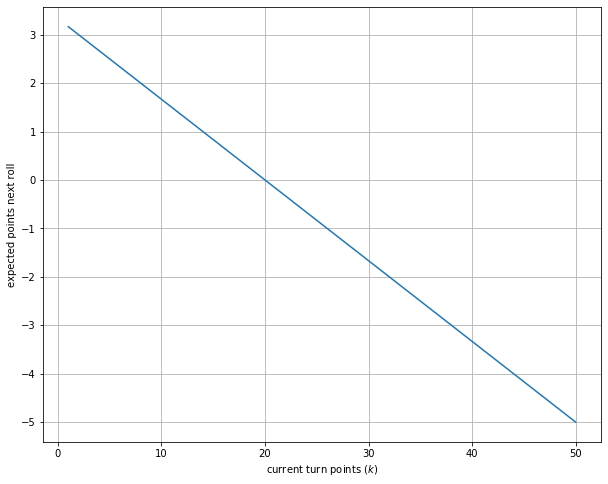
\includegraphics[width=0.7\linewidth]{figures/greedy_pig_expectation}
	\end{center}
\caption{Expected points in the next roll as a function of the current turn points.}
\label{fig:greedy_pig_expec}
\end{figure}
\end{solution}

\begin{question}
Let $X$ be a random variable with density function

\begin{equation*}
f(x) = 
\begin{cases}
k(1 - x^2),~\textrm{if}~0 \leq x \leq 1\\
0,~\textrm{otherwise}		
\end{cases}
\end{equation*}
Find $k$, together with the expectation and the variance of the random variable $Y$ defined as $Y = 3X - 1$.
\end{question}

\cprotEnv\begin{solution}
\label{ex:variance}
To find the value of $k$ we can exploit the normalization condition for a probability density:

\begin{equation*}
\begin{gathered}
\int_\Omega f(x) d\Omega = 1\\
\int_{0}^{1}k(1-x^{2})dx = k\left(x-\frac{1}{3}x^{3}\right|_{0}^{1}= k\left(1-\frac{1}{3}\right) \\
k\left(1-\frac{1}{3}\right) = 1 \implies k = \frac{3}{2}
\end{gathered}
\end{equation*}

The expectation of the variable $Y$ instead equals to
\begin{equation*}
\mathbb{E}[Y] = 3\mathbb{E}[X] - 1
\end{equation*}	
So
\begin{equation*}
\begin{gathered}
\mathbb{E}[X] = \frac{3}{2}\int_{0}^{1}x(1-x^2)dx = \frac{3}{2}\left(\frac{1}{2}x^2-\frac{1}{4}x^{4}\right|_{0}^{1} = \frac{3}{2}\left(\frac{1}{2}-\frac{1}{4}\right) = \frac{3}{8} \\
\mathbb{E}[Y] = 3\cdot\frac{3}{8} - 1 = \frac{1}{8} 
\end{gathered}
\end{equation*}
And finally for the variance:
\begin{equation*}
\begin{aligned}
Var[Y] = & \mathbb{E}[Y^2] - (\mathbb{E}[Y])^2 = \frac{3}{2}\int_{0}^{1}(9x^2 - 6x + 1)(1-x^2)dx - \frac{1}{64} = \\  &\frac{3}{2}\int_{0}^{1}(- 9x^4 + 6x^3 + 8x^2 - 6x + 1)dx - \frac{1}{64} = 
\frac{3}{2}\left(- \frac{9}{5}x^5 + \frac{6}{4}x^4 + \frac{8}{3}x^3 - 3x^2 + x\right|_{0}^{1} - \frac{1}{64} = \\
& \frac{3}{2}\left(- \frac{9}{5} + \frac{6}{4} + \frac{8}{3} - 3 + 1\right) - \frac{1}{64} = \frac{11}{20} - \frac{1}{64} = \frac{171}{320}
\end{aligned}
\end{equation*}

Alternatively it can be demonstrated that the variance of a random variable $Y = a + bX$ can be computed as $Var[Y] = b^2 Var[X]$. Indeed starting from the general form of the variance $Var[Y] = \mathbb{E}[Y^2] - (\mathbb{E}[Y])^2$ and computing each term of the right hand side of the equation 

\begin{equation}
\begin{gathered}
\mathbb{E}[Y^2] = \mathbb{E}[(a+bX)^2] = \mathbb{E}[b^2X^2 + 2abX + a^2] = b^2\mathbb{E}[X^2] + 2ab\mathbb{E}[X]+ a^2  \\
\mathbb{E}[Y]^2 =  (b\mathbb{E}[X] + a)^2 = b^2\mathbb{E}[X]^2 + 2ab\mathbb{E}[X]+ a^2  
\label{eq:each_var}
\end{gathered}
\end{equation}
Substituting Eqs.~\ref{eq:each_var} into the general form of the variance 
\begin{equation}
\begin{gathered}
Var[Y] = b^2\mathbb{E}[X^2] + 2ab\mathbb{E}[X]+ a^2 - (b^2\mathbb{E}[X]^2 + 2ab\mathbb{E}[X]+ a^2) \\ 
= b^2\mathbb{E}[X^2] - b^2\mathbb{E}[X]^2 = b^2 Var[X]
\end{gathered}     
\end{equation}

So $Var[Y] = 9\mathbb{E}[X]$.
\end{solution}

\begin{question}
We want to insure a car of 12000 EUR. The probability that a car is involved in an accident during a year is 0.15 in which case the amount of damage is

\begin{itemize}
\tightlist
\item 20\% of its value with probability 0.8;
\item 60\% of its value with probability 0.12;
\item 100\% of its value with probability 0.08.
\end{itemize}
Find the first annual premium the insurer must charge to have the expected cost of the company equal to 0.
\end{question}

\cprotEnv\begin{solution}
\begin{ipython}
print ("{:.2f} EUR".format(0.15 * 12000 * (0.8*0.2 + 0.6*0.12 + 0.08)))
\end{ipython}
\begin{ioutput}
561.60 EUR
\end{ioutput}
\end{solution}

\begin{question}
The daily expenditure ($X$, in euros) spent by a certain customer in a department store is distributed according to the following density function:

\begin{equation*}
f(x) = 
\begin{cases}
x^2/9000,~\textrm{if}~0 \leq x \leq 30\\
0,~\textrm{otherwise}		
\end{cases}
\end{equation*}

\begin{enumerate}[label={\emph{\alph*})}]
\item calculate the probability that the client has a daily spending between 15 and 20 EUR;
\item what is his/her expected daily expenditure ?;
\item next winter the department store is granting the following "discount vouchers", whose amount depends on the client's expenditure: 1 EUR for spending between 10 and 20 EUR, 1.5 EUR for spending between 20 and 25 EUR,
3 EUR if the expense exceeds 25 EUR. Derive the distribution and the expected value of the discounts obtained by the client.
\item the customer has paid for his/her purchases in the store with a credit card which applies a 4\% charge. What is the probability that the customer has paid (with charges included) between 10 and 15 EUR ?
\end{enumerate}
\end{question}

\cprotEnv\begin{solution}
\begin{enumerate}[label={\emph{\alph*})}]
\tightlist
\item First we need to calculate the CDF by simple integration of the given PDF.
\begin{ipython}
def F(x):
    return x**3/27000

P = F(20) - F(15)
print (P)
\end{ipython}
\begin{ioutput}
0.17129629629629628
\end{ioutput}
\item The expected expense is given by $\int_{0}^{30} xf(x) dx = x^4/36000$
\begin{ipython}
def tot(x):
    return x**4/36000

print (tot(30))
\end{ipython}
\begin{ioutput}
22.5	
\end{ioutput}

\item The expected discount value is given by the weighted average of each discount times the probability of spending the corresponding amount of money:
\begin{ipython}
expected = 1 * (F(20)-F(10)) + 1.5 * (F(25) - F(20)) + 3 * (F(30) - F(25))
print (expected)
\end{ipython}
\begin{ioutput}
1.9467592592592593
\end{ioutput}

\item If the customer spent between 10 and 15 EUR with an extra charge of 4\% (by the usage of the credit card) the real expense limits has to be scaled by $1 - 0.04$, then the corresponding probability can be found using the function \texttt{F}:
\begin{ipython}
xmin = 10*0.96
xmax = 15*0.96
P = F(xmax) - F(xmin)

print (P)
\end{ipython}
\begin{ioutput}
0.07782399999999998
\end{ioutput}
\end{enumerate}
\end{solution}

\cprotEnv\begin{question}
An economist wishes to estimate the total cost of a project. His salary is composed of a fixed part of 12000 EUR plus a variable part of 300 EUR per day of work. The project can be performed between 7 and 11 days, and the economist has derived the following subjective probability distribution for the random variable $X$ (number of days it will take to implement the project):
\begin{ipython}
P = {7:0.10, 8:0.20, 9:?, 10:0.30, 11:0.10}
\end{ipython}
\begin{enumerate}[label={\emph{\alph*})}]
\tightlist
\item What is the probability that the project is carried out in 9 days? Justify your answer.
\item Determine the expected cost of the project and its variance. 
\end{enumerate}
\end{question}

\cprotEnv\begin{solution}
\begin{enumerate}[label={\emph{\alph*})}]
\tightlist
\item Since the assumption is that the work can be completed in between 7 and 11 days, the sum of $P$s has to equal 1. So $P(9)$ can be determined as
\begin{ipython}
P = {7:0.10, 8:0.20, 10:0.30, 11:0.10}
P[9] = 1 - (P[7]+P[8]+P[9]+P[10]+P[11])

print ("{:.2f}".format(P[9]))
\end{ipython}
\begin{ioutput}
0.30
\end{ioutput}
\item The expected cost of the project results
\begin{ipython}
expected_days = sum([d*p for d, k in P.items()])
E_C = 12000 + 300*expected_days

print (E_C)
\end{ipython}
\begin{ioutput}
14730.0	
\end{ioutput}

Remembering Solution~\ref{ex:variance} the variance in the costs $Var[C]$ (which follows a linear relationship with the number of days $C = 12000 + 300\cdot d$) becomes
\begin{ipython}
var_days = sum([(d**2)*p for d, k in P.items()])
b = 300
print (b**2 * var_days)
\end{ipython}
\begin{ioutput}
116100.0	
\end{ioutput}
\end{enumerate}
\end{solution}

\begin{question}
A casino advertises that the expected prize won by its clients is 600 EUR, with risk $\sigma$ = 360.
\begin{enumerate}[label={\emph{\alph*})}]
\tightlist
\item Calculate the probability that a player wins between 150 and 1050 EUR.
\item How would the above probability change if $\sigma$ = 420 ?
\item What is the probability that the prize won by a player deviates at least 504 EUR from its expectation?
\end{enumerate}
\end{question}

\cprotEnv\begin{solution}
In this case it is safe to assume that the wins are distributed as a Gaussian with mean 600 EUR and standard deviation 360 EUR. 
\begin{enumerate}[label={\emph{\alph*})}]
\tightlist
\item It is much easier to convert the initial distribution to a standard normal (zero mean and unit variance) using the following transformation
\begin{equation*}
x' = \frac{(x - \mu)}{\sigma}
\end{equation*}
in such a way \texttt{scipy.stats.norm} can be used.

\begin{ipython}
from scipy.stats import norm

# convert the two limits in the standard normal
xmin = (150 - 600)/360
xmax = (1050 - 600)/360

print (xmin, xmax)
print (norm.cdf(xmax) - norm.cdf(xmin))
\end{ipython}
\begin{ioutput}
-1.25 1.25
0.7887004526662893
\end{ioutput}

\item If the risk (i.e. uncertainty) increases the probability of winning an amount of money in the same range is expected to decrease. Let's check using the same technique as in the previous answer.
\begin{ipython}
xmin = (150 - 600)/420
xmax = (1050 - 600)/420

print (xmin, xmax)
print (norm.cdf(xmax) - norm.cdf(xmin))
\end{ipython}
\begin{ioutput}
-1.0714285714285714 1.0714285714285714
0.7160232282490884
\end{ioutput}

Indeed now the range has shrunk from $\pm1.5\sigma$ to $\pm1.07\sigma$. 

\item Finally, we can determine the probability that a win exceeds 504 EUR the mean in a similar fashion.

\begin{ipython}
xmin = 504/360

print (xmin)
# the factor 2 because the win can exceed both ways the mean
print (norm.cdf(-xmin) * 2)
\end{ipython}
\begin{ioutput}
1.4
0.16151331846754213
\end{ioutput}
\end{enumerate}
\end{solution}


\chapter{Interpolation, Root Finding and Minimization}
\label{sec:interpolation}

In this Chapter some very important mathematical tools will be reviewed. These will be intensively used later on throughout this book.

\section{Linear Interpolation}
\label{linear-interpolation}

Consider to have recorded the value of a quantity at three points in time as in Fig.~\ref{fig:samples_for_interpolation}.
Starting from this small data sample we can infer the value of this quantity at different times using the \emph{interpolation} technique. Clearly this is 
possible only under certain assumptions that will be described along with the example.

\begin{figure}[htbp]
  \centering
  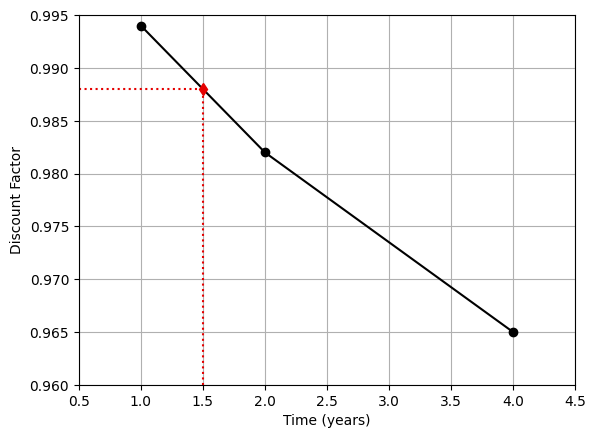
\includegraphics[width=0.7\textwidth]{figures/interp_example1}
  \caption{Plot of the discount curve described in the text.}
  \label{fig:samples_for_interpolation}
\end{figure}

Given two sample points $d_1$ and $d_2$ taken at two different times $t_1$ and $t_2$ a new value, between these two, can be found as the point lying on the 
\textbf{line} connecting $d_1$ and $d_2$ at the desired time. Here the main assumption is that the quantity is changing \textbf{linearly} with the time in the
interval $[t_1, t_2]$.

\begin{attention}
\subsubsection{Derivation}
The equation of a line for two points $(t_1, d_1)$ and $(t_2, d_2)$ can be written as:

\begin{equation}
\frac{t - t_1}{t_2 - t_1} = \frac{d - d_1}{d_2 - d_1}
\end{equation}

Setting $w = \cfrac{t - t_1}{t_2 - t_1}$ and solving for $d$ we find the desired solution:

\begin{equation}
(d_2 - d_1)\cdot w = d - d_1\quad\implies\quad d = (1 - w)\cdot d_1 + w \cdot d_2
\end{equation}

This formula can be interpreted as a weighted average where the weights are inversely related to the distances from the end points to the unknown 
point ($w_1 = (1 - w) = \cfrac{t_2 - t}{t_2 -t_1}, w_2 = w$), which means that the closer point has more "influence" than the farther point on the result.
\end{attention}

Although quite simple, you don't need to implement the interpolation formula from scratch, instead it can be used the one provided in 
\texttt{scipy.interpolate.interp1d}. 

\pythoncodenon{code/discount_1.py}

\begin{ioutput}
0.988
\end{ioutput}

\textbf{Always interpret critically your results to guess if they make sense or not and avoid mistakes}. In the previous example we certainly expected something between 0.994 and 0.982 (our range ends) furthermore since we are looking for the value at a time which is halfway the considered interval, the result will be somehow in the middle of $d_1$ and $d_2$ ($\approx 0.988$). This simple kind of reasoning should be applied every time you have a result to quickly judge it.

\begin{curiosity}
\subsubsection{Epic Failure}
The Mars Climate Orbiter \emph{was} a 638~kg (1,407~lb), 326.7~M\$ space probe launched by NASA on December 11, 1998 to study Martian climate, atmosphere, 
and surface changes. 

On September 15, 1999, the necessary corrections to speed and direction of the probe were computed in order to place the spacecraft at an optimal position 
for an orbital insertion maneuver that would bring it around Mars at the proper altitude. 
But one week later communication with the spacecraft was permanently lost as it went into Martian orbital insertion. 

A committee of experts was created to investigate the reasons of 
such failure and they found out that the spacecraft encountered Mars at a lower than foreseen altitude causing either its destruction by atmospheric 
friction or making it bouncing against the atmosphere re-entering heliocentric orbit after leaving Mars.

The primary cause of this discrepancy was found in one piece of software (supplied by Lockheed Martin) that produced results in "Imperial" units, 
while a second system (supplied by NASA) expected those results to be in SI units. Specifically, the software calculated the total impulse produced by 
thrust in \emph{pound-force seconds}. The trajectory calculation software then used these results, expected to be in \emph{newton seconds}, thus 
incorrect by a factor of 4.45, to update the predicted position of the spacecraft.
	
NASA took the entire responsibility for having vaporized about 300~M\$ in the Martian atmosphere, mainly for failing to make the appropriate checks and 
tests that would have caught this unit discrepancy~\cite{bib:mars}.	
\end{curiosity}

\subsubsection{Extrapolation Issue}

Interpolation is primarily designed to estimate values \textbf{within} the range of known data points. Attempting to extrapolate beyond the data range can lead to inaccurate results and is generally discouraged. 

Extrapolation assumes that the relationship between data points remains true \emph{forever}, which may not be valid in general.

Indeed if this assumption is not correct you can simple ask $\texttt{python}$ to raise an error to avoid misleading results using the \texttt{bounds\_error} option
\begin{ipython}
interpolator = interp1d(t, dfs, bounds_error=True)
\end{ipython} 

\subsection{Log-linear Interpolation}
\label{log-linear-interpolation}

When there is an exponential connection between the two variables (e.g. $t$ and $p$) we can fall back to the linear case by a simple transformation. 
Imagine that $p=e^{-rt}$, applying the logarithm to both sides of the equation gives:

\begin{equation}
f = \log(p) = \log(\exp(-rt)) = -rt
\end{equation}
so there is a linear relation between the new variable $f$ and $t$. At this point we can use the results of the previous Section to interpolate for values of $f$, just remember to exponentiate the final result to get the correct value of $p$.

\pythoncodenon{code/interp_1.py}

\begin{ioutput}
0.988
\end{ioutput}

\subsection{Limitations of Interpolation}
Interpolation is just an approximation and it can be easily demonstrated that the underlying linear approximation of a function $f(x)$ gets worse as the second derivative of the function ($f''(x)$). 

This is intuitively correct: the "curvier" the function, the worse the approximation made with simple linear interpolation, see Fig.~\ref{fig:sine_interp}.

\begin{figure}
  \centering
  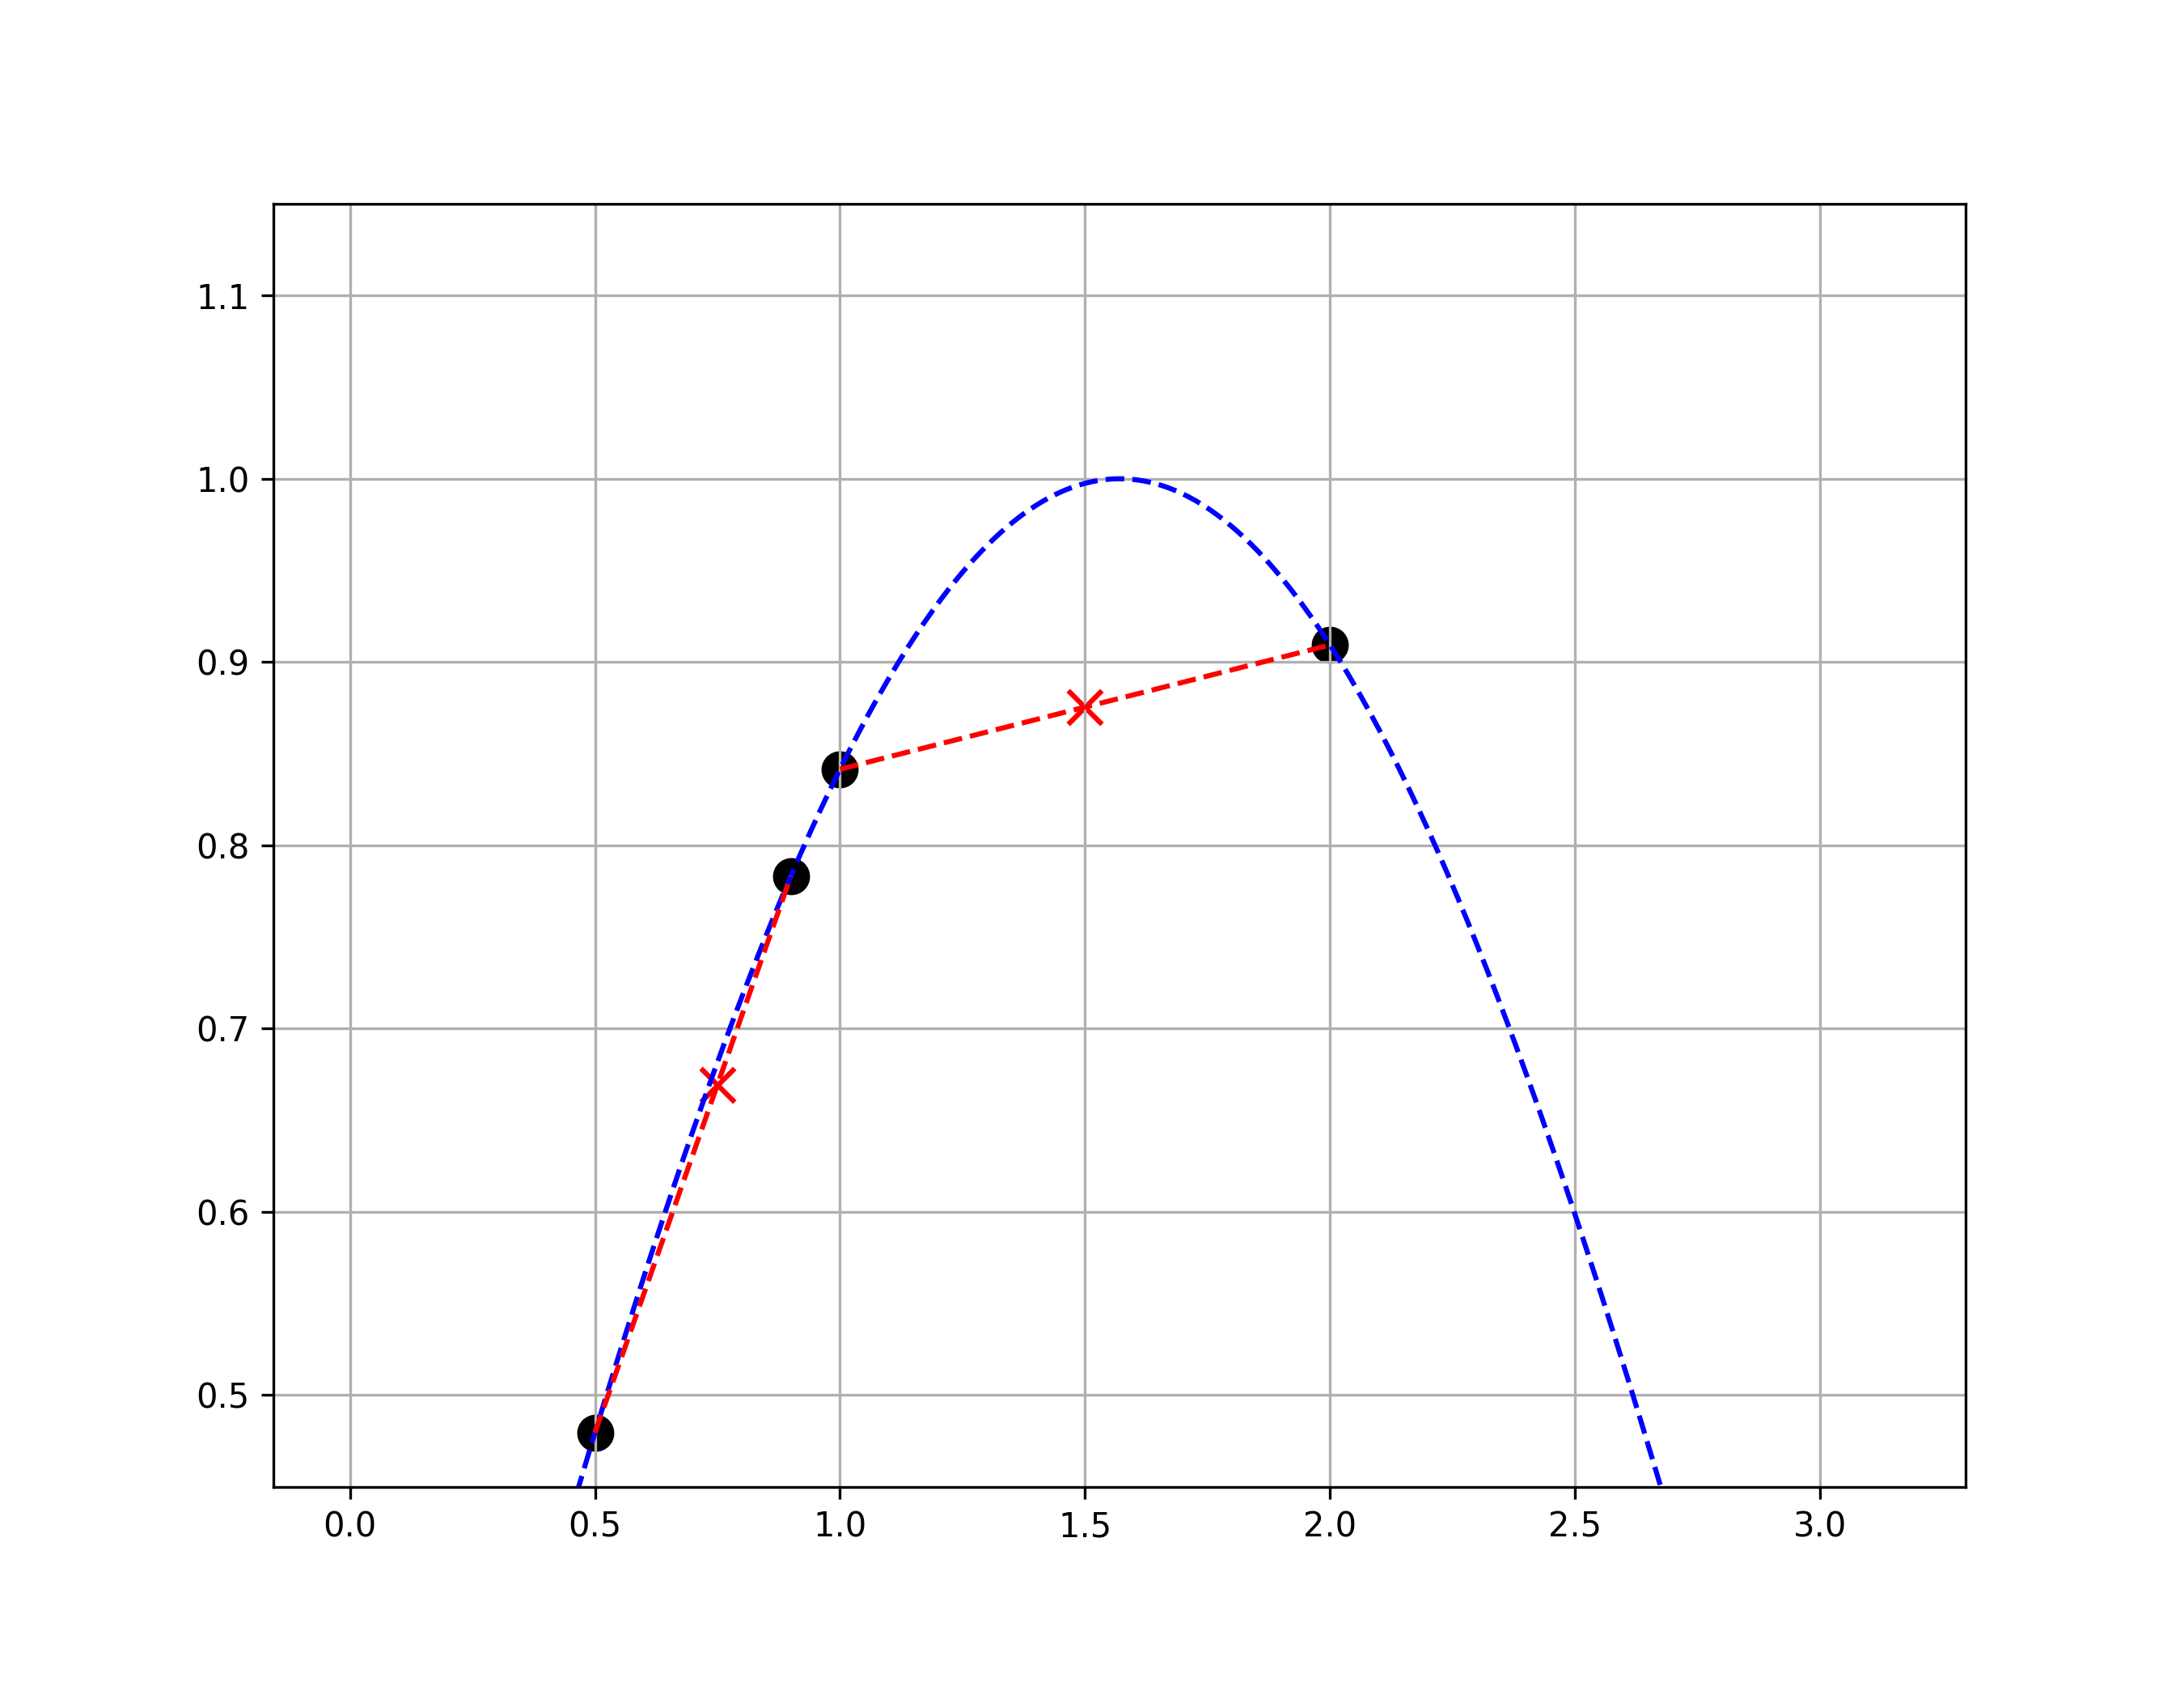
\includegraphics[width=0.7\textwidth]{figures/wrong_interp.png}
  \caption{Trying to approximate a sine function with a line is clearly not going to work unless the interpolation interval is very small.}
  \label{fig:sine_interp}
\end{figure}

To improve the approximation accuracy e.g. in the evaluation of natural logarithm or trigonometric functions, higher order polynomials can be used ($p(x)=a_0 + a_1\cdot x + a_2\cdot x^2+\cdots$). It has to be clear however that going to higher degrees does not always help~\cite{bib:runge}.
Some interpolation methods, indeed, can result in \emph{overfitting}. This means the interpolating function fits the data points very closely but may not generalize well to unseen data, i.e. it can lead to excessive fluctuations between data points.

\section{Root Finding}
\label{sec:root_finding}

To find the zeros of a function $f(x)$ means to determine the values $\hat{x}$ such that $f(\hat{x})=0$ and the process is equivalently called "finding the roots of $f(x)$". Below we are going to review few methods to perform root finding.

\subsection{Bisection}
\emph{Bisection}~\cite{bib:bisection} method is considered the simplest one-dimensional root-finding algorithm.

Suppose we know two points of an interval $[a,b]$ (see Fig.~\ref{fig:bisection}), and that $f(a)< 0$ and $f(b)> 0$. Since the value of $f(a)$ is negative and $f(b)$ is positive, we are certain that at least one root $x$ lies somewhere between $a$ and $b$.

Taking the midpoint of the $[a, b]$ interval, say $c$, the algorithm evaluates the value $f(c)$. If $f(c) \simeq 0$ within some predetermined tolerance, then a root has been found. If $f(c)< 0$, then we may conclude that a root exists along the interval $[c, b]$, or along $[a,c]$ otherwise.

On the next evaluation, $c$ is replaced as either $a$ or $b$ accordingly. With the new interval shortened, the bisection method repeats with the same evaluation to determine the next value of $c$. This process continues, shrinking the width of the interval until the root is found.

\begin{figure}[htbp]
\centering
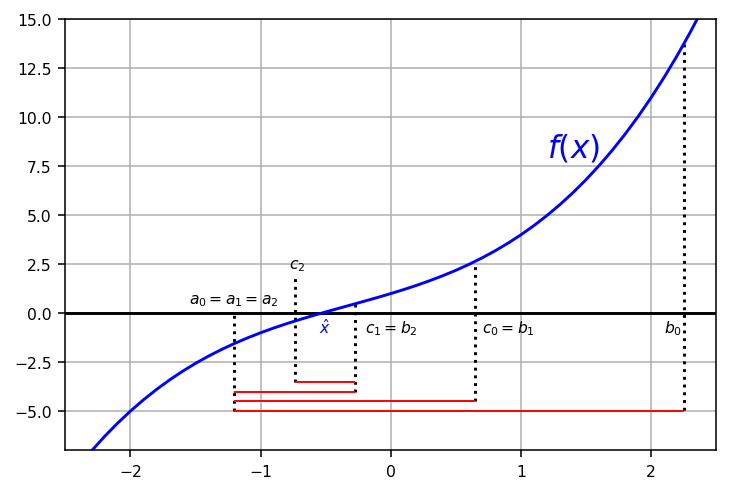
\includegraphics[width=0.7\linewidth]{figures/bisection}
\caption{Example of bisection algorithm to find the roots of a function $f(x)$.}
\label{fig:bisection}
\end{figure}

The biggest advantage of the bisection method is it is guaranteed to converge to, at least, an approximation of the root. It should be noted that it does not require knowledge of the derivative of the unknown function $f(x)$, which in certain cases could be complex or even impossible to calculate. This makes this method extremely valuable for working on functions that are not smooth.
Contrary, its major drawback is that it takes up more computational time in the iterative evaluation as compared to other methods. 

We can implement the bisection method with \texttt{scipy.optimize.bisect} (for the usage of \texttt{args} see Section~\ref{sec:kwargs_args}).

\begin{ipythonnon}
from scipy.optimize import bisect 

def f(x, a, b, c):
    return a*x**2 + b*x + c 
  
print (bisect(f, -3, 3, args=(1, -8, 4)))
\end{ipythonnon}
\begin{ioutput}
0.5358983848632306
\end{ioutput}

An alternative algorithm is the \emph{Brent's method}~\cite{bib:brent} which combines the advantages of both bisection and secant (another root-finding algorithm) methods. Its \texttt{python} implementation is \texttt{scipy.optimize.brentq}.

\begin{ipythonnon}
from scipy.optimize import brentq
    
print (brentq(f, -3, 3, args=(1, -8, 4)))
\end{ipythonnon}
\begin{ioutput}
0.5358983848622614
\end{ioutput}

\noindent
The results match down to the eleventh digit.

\subsection{Newton-Raphson Method}

Newton's method is a root-finding algorithm which produces successively better approximations to the roots (or zeroes) of a real-valued function. 

The algorithm starts by choosing an initial guess $x_0$, then approximating the function with its tangent ($g(x)$), 
\begin{equation*}
g(x) = f(x_0) + \cfrac{\partial f}{\partial x}(x_0)(x - x_0)
\end{equation*}
and finally computing the $x$-intercept of this tangent line. The intercept will typically be a better approximation to the original function's root than the first guess, and the method can be iterated.

Suppose the tangent to $f(x)$ at $x = x_n$ intercepts the $x$-axis at $x_{n+1}$ then we have two cases:
\begin{enumerate}
\item the original function value in $x_{n+1}$ is "close enough" to 0 such that we are fine with this approximated solution e.g. $f(x_{n+1}) < \texttt{tol}=10^{-8}$. In this case we are done and the algorithm stops;
\item otherwise we need to solve for $x_{n+1}$ and iterate the process again
\begin{equation*}
g(x_{n+1}) = f(x_n) + \cfrac{\partial f}{\partial x}(x_n)(x_{n+1} - x_n) = 0
\end{equation*}
from which we get
\begin{equation*}
f(x_{n})-0 = f'(x_n)(x_{n}-x_{n+1}) \Rightarrow x_{n+1}=x_n-\frac {f(x_n)}{f'(x_n)}
\end{equation*}
\item Another iteration is then started from $x_{n+1}$.
\end{enumerate}

The method will usually converge, provided the initial guess is close enough to the unknown zero, and $f'(x_0) \neq 0$.
\begin{center}
	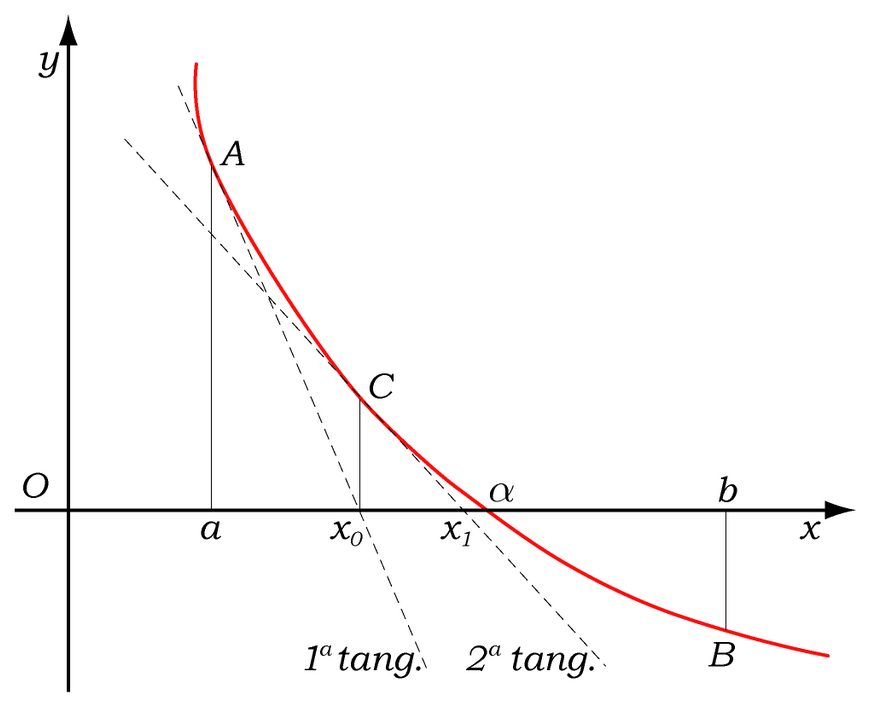
\includegraphics[width=0.6\linewidth]{figures/newton_method}
\end{center}

\begin{ipythonnon}
from scipy.optimize import newton 

def f(x, a, b, c):
    return a*x**2 + b*x + c 
  
print (newton(f, 1, args=(1, -8, 4)))
\end{ipythonnon}
\begin{ioutput}
0.5358983848622547
\end{ioutput}

\section{Minimization  Algorithm}
\label{sec:minimization-algorithm}

Minimization algorithms are fundamental tools across various scientific and engineering disciplines, playing a crucial role in finding the best possible solutions to problems by systematically reducing a defined \emph{objective function}. Whether it's minimizing energy in physics, cost in economics, error in machine learning models, or resource usage in operations research, these algorithms iteratively search through a solution space to locate the point 
that yields the smallest value of the function being optimized. 

Their importance lies in enabling us to automate the process of finding optimal or near-optimal solutions to complex problems that would be intractable to solve manually, leading to more efficient processes, better predictions, and improved designs.

\subsection{The Algorithm}
The minimization algorithm follows these steps:

\begin{itemize}
\tightlist
\item define an \emph{objective function} i.e. the function that has to be minimized;
\item set the initial value of the unknown parameters ($\mathbf{x_0}$) and their range of variability (those are the parameters that will be changed to find  the objective function minimum);
\item compute the objective function value;
\item move the parameter values to find a smaller value of the objective function (e.g. following the derivative direction w.r.t. each parameter); in case constraints are defined, they will be considered when the parameter values are varied;
\item repeat the previous two steps until further variations of $\mathbf{x}$ won't change significantly the objective function (i.e. we have found a minimum of the function so the minimization process is completed !).
\end{itemize}

Let's see with a couple of examples how minimization can be implemented in \texttt{python} using the function \texttt{scipy.optimize.minimize}.

\subsubsection{Reducing the Production Costs}
\label{example}

Let's determine the optimal size of a circular cylindrical can of volume, $330~\mathrm{cm}^3$, that minimizes the cost of manufacture, see Figure~\ref{fig:cylinder}.

\begin{figure}[ht]
\centering
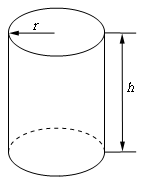
\includegraphics[width=0.2\textwidth]{figures/cylinder.png}
\caption{Graphical representation of the \emph{can} minimization example.}
\label{fig:cylinder}
\end{figure}

To minimize the costs, you need to reduce the amount of alluminum used, consequently the can surface. The objective function is given by the area of the cylinder (the can is assumed to be smooth to simplify the calculation). On the other hand the can volume is fixed to 33~cl (or 330~$\mathrm{cm}^3$) so we get a system of two equations

$$
\begin{cases}
S = 2\pi rh + 2\pi r^2 \\
V = \pi r^2 h = 330\quad\implies h = \cfrac{330}{\pi r^2}
\label{eq:can_surface}
\end{cases}
$$
Replacing $h$ in the first equation leads to

\begin{equation}
S = 2\pi rh + 2\cdot(\pi r^2) = \cfrac{2\cdot 330}{r} + 2\cdot(\pi r^2)
\end{equation}
The objective function depends on one parameter only \texttt{x[0]} which is the can radius. We are going to use a \texttt{list} (or a \texttt{numpy.array}) even if we deal with one parameter so that the same code can be generalized to more complex problems with a larger number of parameters.
Set the limits to our unknown variable and its initial value and finally run the minimization.

\pythoncodenon{code/interp_2.py}
\begin{ioutput}
  message: CONVERGENCE: NORM OF PROJECTED GRADIENT <= PGTOL
  success: True
   status: 0
      fun: 264.35681091484054
        x: [ 3.745e+00]
      nit: 9
      jac: [ 0.000e+00]
     nfev: 24
     njev: 12
 hess_inv: <1x1 LbfgsInvHessProduct with dtype=float64>       
\end{ioutput}

Printing the result gives us the a lot of information about the minimization just performed, the most useful are:
\begin{itemize}
\item \texttt{fun}: the objective function value at the last iteration;
\item \texttt{message}: the summary message (if it is \texttt{CONVERGENCE} is almost always OK);
\item \texttt{success}: the name is self explanatory;
\item \texttt{status}: should be 0;
\item \texttt{x}: the vector of unknown parameters that have been optimized.
\end{itemize}

Referring to Fig.~\ref{fig:minimization_diagnostic} it can be understood how minimization works, each step of the minimization is shown along the objective function down to the minimum. Notice that the surface is a quadratic function of the radius so it is guaranteed to have just one minimum.

\begin{figure}[htb]
\centering
%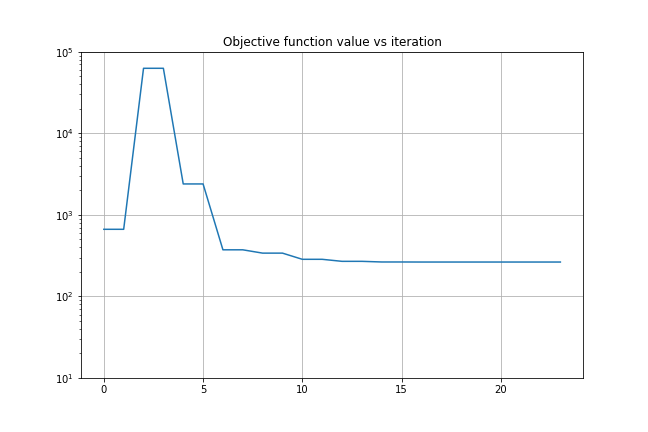
\includegraphics[width=0.45\linewidth]{figures/objective_function_value}
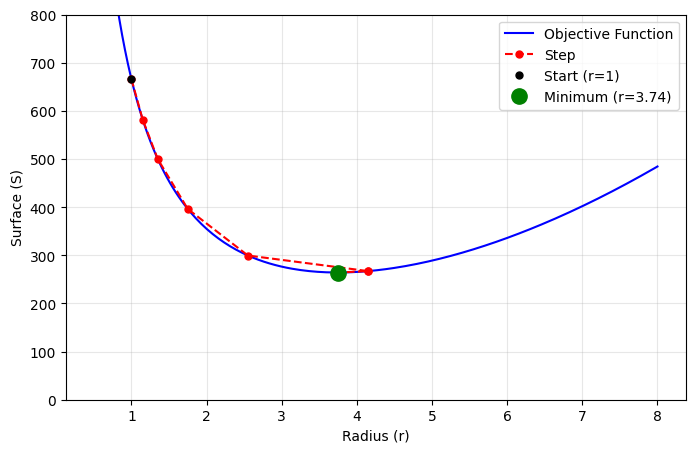
\includegraphics[width=0.80\linewidth]{figures/can_surface_2}
\caption{Diagnostic plot for the minimization algorithm. The parameter $x[0]$ starts with the initial value $1$ then it is adjusted at each iteration in order to reduce the can surface.}
\label{fig:minimization_diagnostic}
\end{figure}

Going back to the result it looks like that to minimize production costs the can radius has to be about 3.7~cm (or about 75~mm diameter).

\begin{curiosity}
It looks like Coca Cola has done a similar calculation since the result is surprisingly close to that of a real can. 

From \href{	https://www.ball.com/eu/solutions/markets-capabilities/capabilities/beverage-cans/standard-range
}{here} seems that a real can has a 66.3~mm diameter, a little smaller than our but it is not surprising since the real can shape is more elaborated than a 
simple cylinder.
\end{curiosity}

\subsection{Parameter Update Techniques}

\subsubsection{Gradient Descent Limitations}
During the iterations of the minimization algorithm the parameter update is done following directly the \textit{gradient} (i.e. first derivative) scaled by the \textbf{learning rate}

\begin{equation}
\theta_i^{(t+1)} = \theta_i^{(t)} - \alpha \frac{d}{d\theta}L(\theta_i^{(t)})
\end{equation}

This method has some limitations though:
\begin{itemize}
	\item is slow for large samples;
	\item the learning rate (step size) is important. Too big, and we overshoot. Too small, and we crawl.
\end{itemize}

\subsubsection{Newton's Method: A Second-Order Approach}

Newton's method is faster than Gradient Descent. As we have seen before it uses the Hessian matrix which gives information about the curvature of the loss function.

Starting from the second-order Taylor expansion around the current point $t$:
$$
L(\theta_i^{(t)})\approx L(\theta_i^{(t)})+L'(\theta_i^{(t)})s+\frac{1}{2}L''(\theta_i^{(t)})s^2
$$
where $s$ is the step.

To find the minimum, we set the derivative with respect to the step $s$ to zero:
$$
\begin{gathered}
	\frac{d}{ds}\left[L(\theta_i^{(t)})+L'(\theta_i^{(t)})s+\frac{1}{2}L''(\theta_i^{(t)})s^2\right]=0\\
	L'(\theta_i^{(t)})+L''(\theta_i^{(t)})s=0
\end{gathered}
$$
Solving for the optimal step $s_k$:
$$
s_k=-\frac{L'(\theta_i^{(t)})}{L''(\theta_i^{(t)})}
$$
the Newton's update is:

$$
\theta_i^{(t+1)} = \theta_i^{(t)} - \alpha \frac{L'(\theta_i^{(t)})}{L''(\theta_i^{(t)})}
$$

This method has some drawbacks too: calculating and inverting the Hessian is costly. This is especially true for big models (e.g. neural networks), where indeed Gradient Descent is used.

\subsection{Constrained Minimization (aka Fencing a Field)}
\label{example-with-constraint}

Imagine to fence a rectangular field. If we look at the field from above the vertical sides fence cost is 10~EUR/m, the bottom side cost is 2~EUR/m and that of the top side is 7~EUR/m. If we have a 700~EUR budget determine the field dimensions that will maximize the enclosed area, see Fig.~\ref{fig:field}.

\begin{figure}[ht]
\centering
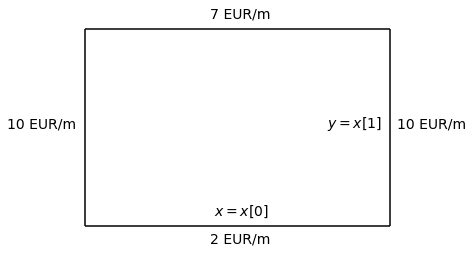
\includegraphics[width=0.5\textwidth]{figures/field.png}
\caption{Graphical representation of the \emph{field} minimization example.}
\label{fig:field}
\end{figure}

In this example there are two differences with respect to the previous:

\begin{itemize}
\tightlist
\item we want to \emph{maximize} a quantity rather than to minimize;
\item there is a constraint (we have a limited budget).
\end{itemize}

\pythoncodenon{code/interp_3.py}

The objective is to maximize the enclosed area $A$ but our algorithm can only minimize functions. To overcome this issue the objective function can be defined to return the quantity $-A$, so that minimizing its value, the real objective, $A$, is maximized. 
Define the field length and width as two items of an array \texttt{x]}, then set their boundaries, their initial values (1~m each) and each side cost and total budget.

Finally we have to impose the budget constraint. This is done by defining a function that computes the fence cost and compare it to the total budget. The constraint is passed to the minimizer as a dictionary (or a list  of dictionaries if there are more) with three keys: \texttt{type}, here set to \texttt{'eq'} (i.e. equality, since we want to spend all of our available money so the fence has to cost \textbf{exactly} 700~EUR), \texttt{'fun'} 
which defines the constraint function and \texttt{'args'} which is optional and set to a tuple whose items are possible additional parameters needed by the constraint function.

The constraint is then defined as
\begin{equation*}
\mathrm{budget} - \mathrm{fence~cost} = \mathrm{budget} - 2\cdot l\cdot\mathrm{side\_cost} - w\cdot(\mathrm{up\_cost} + \mathrm{down\_cost}) = 0
\end{equation*}

The optimization result tells us that the field has to be 17.5~m long and 38.9~m wide for a total field area of 680.5~$\textrm{m}^2$.

\subsection{Why the Sum of Squared Residuals}
	
Imagine you need to find a single constant value, $c$, that best "fits" the following three data points: $y_1=1$, $y_2=2$, and $y_3=9$.

\subsubsection{Wrong Objective Function: Simple Sum of Residuals}
Use an objective function which is the sum of the signed errors:

$$L_1(c) = \sum_{i} (y_i - c)$$
Let's compute by hand few values of $L_1$ with different candidates for the parameter $c$.

\begin{table}[h]
	\centering
	\begin{tabular}{cccl}
		\toprule
		\textbf{Candidate $c$} & \textbf{Errors $(y_i - c)$} & \textbf{$J_1(c)$} & \textbf{Problem} \\
		\midrule
		\textbf{3} & -2, -1, +6 & $3$ & \textbf{High total error magnitude.} \\
		\textbf{4} (True Mean) & -3, -2, +5 & $\mathbf{0}$ & \textbf{Deceptively low.} \\
		\textbf{10} & -9, -8, -1 & $-18$ & \textbf{Worst fit, but the function suggests going lower.} \\
		\bottomrule
	\end{tabular}
\end{table}

\begin{ipythonnon}
import numpy as np

from scipy.optimize import minimize

data = np.array([1, 2, 9])

def wrong_obj_function(x):
  return np.sum(data-x)

x0 = np.array([100])
opts = minimize(wrong_obj_function, x0)
print (opts)
\end{ipythonnon}
\begin{ioutput}
  message: Desired error not necessarily achieved due to precision loss.
  success: False
   status: 2
      fun: -5.029350242370365e+26
        x: [ 1.676e+26]
      nit: 8
      jac: [-3.000e+00]
 hess_inv: [[-1.194e+34]]
     nfev: 1790
     njev: 889
\end{ioutput}

If you use the \textbf{simple sum of errors} as the objective function, the optimal $c$ is \textit{undefined} because positive and negative errors cancel out. In practical terms, it always leads to a derivative that is a constant, which gives \textbf{no meaningful minimum}.

For example, a terrible fit like $c=100$ would only appear a better choice because the negative numbers dominate, but $L_1(c)$ doesn't accurately reflect the \textbf{true total distance of the points} from $c$.

\subsubsection{Right Objective Function: Sum of Squared Residuals}

Use an objective function with the sum of the squared errors:
$$L_2(c) = \sum_{i} (y_i - c)^2$$
We want to find $c$ that minimizes now $L_2(c)$.

\begin{table}[h]
	\centering
	\begin{tabular}{cccl}
		\toprule
		\textbf{Candidate $c$} & \textbf{Squared Errors $(y_i - c)^2$} & \textbf{$J_2(c)$} & \textbf{Result} \\
		\midrule
		\textbf{3} & $4, 1, 36$ & $41$ & High cost. \\
		\textbf{4} (True Mean) & $9, 4, 25$ & $\mathbf{38}$ & \textbf{The true unique minimum.} \\
		\textbf{10} & $81, 64, 1$ & $146$ & High cost. \\
		\bottomrule
	\end{tabular}
\end{table}

\begin{ipythonnon}
def right_obj_function(x):
  return np.sum((data-x)**2)

x0 = np.array([100])
opts = minimize(right_obj_function, x0)
print (opts)
\end{ipythonnon}
\begin{ioutput}
  message: Optimization terminated successfully.
  success: True
   status: 0
      fun: 38.0
        x: [ 4.000e+00]
      nit: 4
      jac: [ 0.000e+00]
 hess_inv: [[ 1.667e-01]]
     nfev: 14
     njev: 7
\end{ioutput}

By \textbf{squaring the errors}, all terms become positive, \textbf{eliminating the cancellation problem}. The objective function $L_2(c)$ now accurately represents the total magnitude of the error.

When you minimize $L_2(c)$ (by setting the derivative with respect to $c$ to zero), you are guaranteed to find the unique minimum at the \textbf{arithmetic mean} of the data, $c=4$, which is the correct and meaningful best-fit constant.

\subsection{Local Minima}
Minimization problems can be very nasty. For example when the objective function has various local minima, the parameter initial value choice can be critical. 
Assume we would like to minimize something like Fig.~\ref{fig:local_minima}

\begin{equation*}
f(x) = \cfrac{\mathrm{cos}(3\pi x)}{x}
\end{equation*}

\begin{figure}[htb]
	\centering
	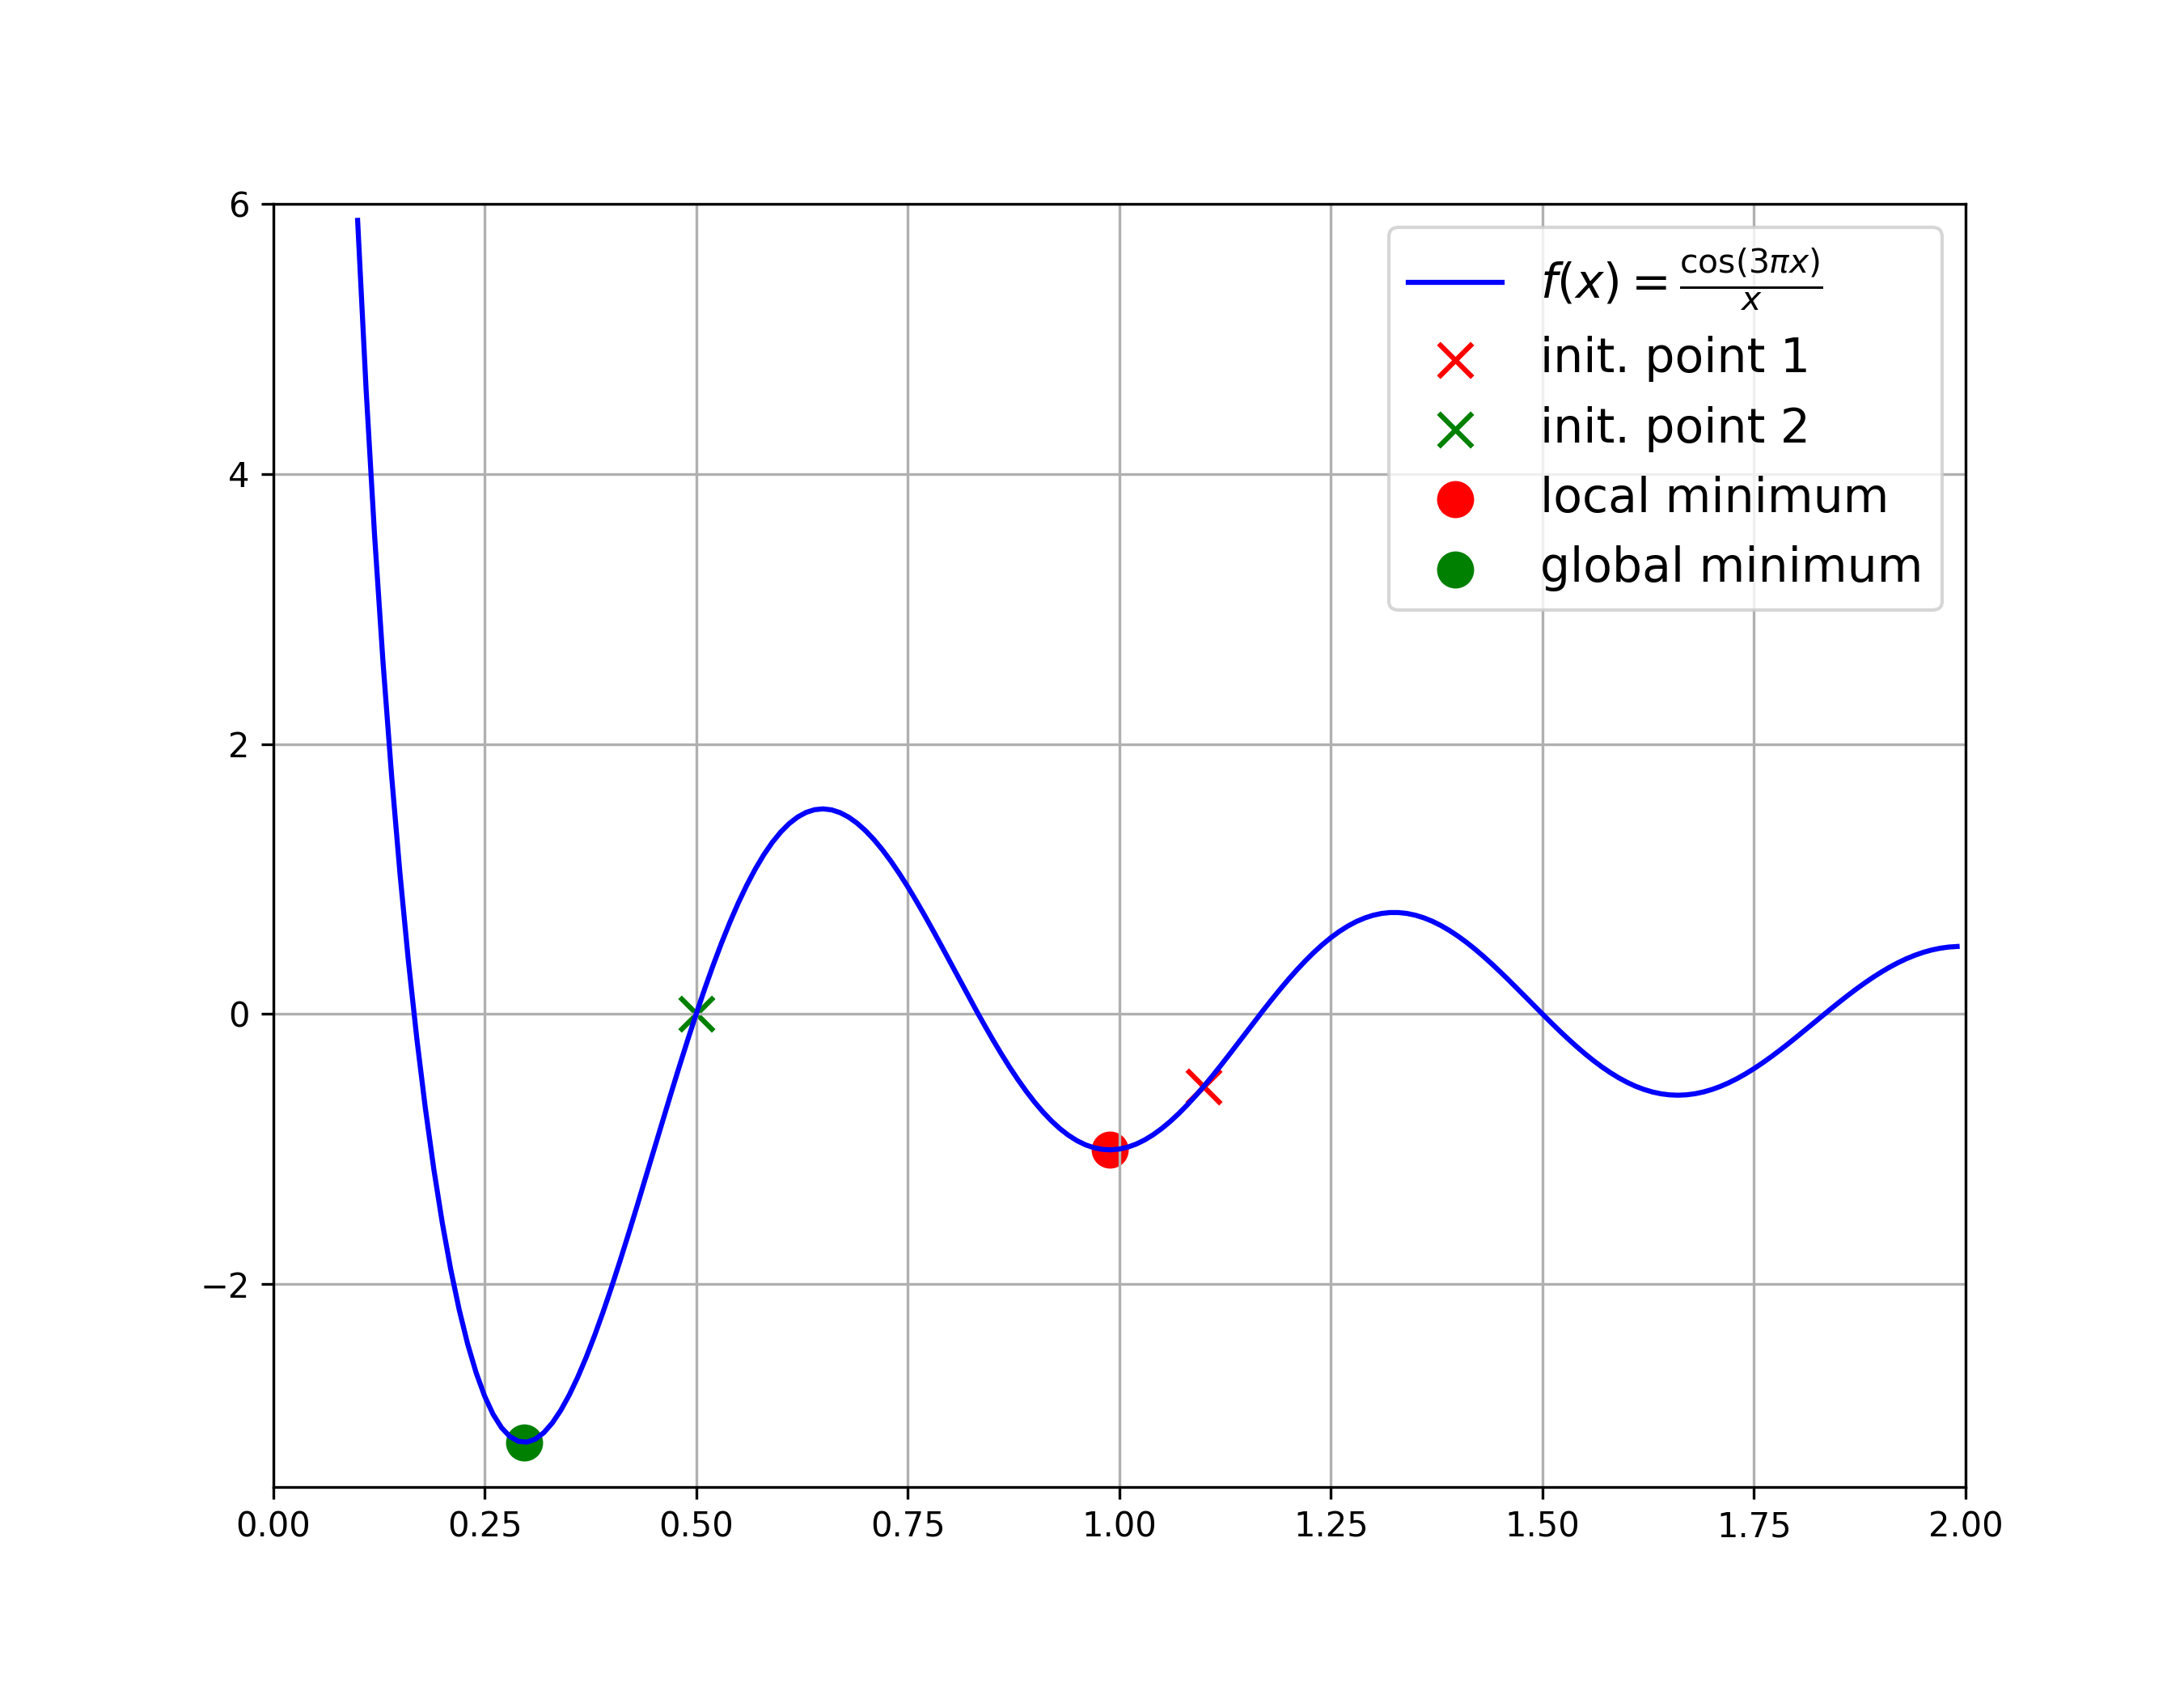
\includegraphics[width=0.7\textwidth]{figures/local_minima}
	\caption{Plot of an example function with many local minima. The red points highlights initial value and minimum found in a \emph{bad} minimization, green points for a good minimization.}
	\label{fig:local_minima}
\end{figure}
Let's try to find a minimum setting the initial value to $x=1.1$.
\begin{ipythonnon}
x0 = [1.1]
bounds = [(0.01, 20)]
r = minimize(func, x0, bounds=bounds)

print (r)
\end{ipythonnon}
\begin{ioutput}
  message: CONVERGENCE: NORM OF PROJECTED GRADIENT <= PGTOL
  success: True
   status: 0
      fun: -1.005698713865489
        x: [ 9.887e-01]
      nit: 5
      jac: [-4.441e-07]
     nfev: 16
     njev: 8
 hess_inv: <1x1 LbfgsInvHessProduct with dtype=float64>
\end{ioutput}
The minimization worked perfectly and we found $x=0.9887$ (i.e. the red point in Fig.~\ref{fig:local_minima}) but this is not the absolute minimum we 
were expecting to find. The algorithm, following the derivative direction, has got stuck in the local minimum without any possibility to jump out the well.

If we repeat the minimization using as initial value $0.5$ instead
\begin{ipythonnon}
x0 = [0.5]
bounds = [(0.01, 20)]
r = minimize(func, x0, bounds=bounds)

print (r)
\end{ipythonnon}
\begin{ioutput}
  message: CONVERGENCE: NORM OF PROJECTED GRADIENT <= PGTOL
  success: True
   status: 0
      fun: -3.171517111385885
        x: [ 2.969e-01]
      nit: 5
      jac: [ 8.882e-07]
     nfev: 16
     njev: 8
 hess_inv: <1x1 LbfgsInvHessProduct with dtype=float64>
\end{ioutput}
Now clearly the algorithm found the absolute minimum in $x=0.2969$ (i.e. the green point in Fig.~\ref{fig:local_minima}).

This is just an example of what could happen when minimizing a function. When dealing with complicated cases it is possible to make a \emph{scan} of the objective function to try to approximately determine where the global minimum is and choose suitable initial values of the guess parameters.

%\section*{Exercises}

\chapter{Discount Factors and Forward Rates}

In this Chapter we begin to see some financial \texttt{python} applications, in particular we are going to deal with discount curves and forward rates.

\section{Discounting}
\label{discount-factors}

The core principle of \emph{time value of money} states that a dollar today is worth more than a dollar tomorrow. This is because money has the potential to earn interest over time.
The concept acknowledges that the ability to invest and grow your money today holds more value than receiving the same amount later.

\emph{Discounting} is the process of determining the present value of a future cash flow. It essentially takes the future amount and adjusts it downward to reflect its current worth based on the time value of money, i.e. a chosen discount rate.

With $D(T)$ (or $D(0,T)$) it is represented the discount factor corresponding to a spot rate $r$, and a future time $T$ (in year fraction). 

Consider a payment $N$ that is to be made $T$ years in the future, we calculate the present value ($PV$) as

\begin{equation}
PV = N\cdot D(T) = N \cdot \cfrac{1}{(1 + r)^t}~~~~~
(N \cdot e^{-rt}~~~\text{continuous compounding})
\label{eq:discount_factor}
\end{equation}

The discount rate $r$ which is used in financial calculations is usually chosen to be equal to the cost of capital, i.e. the risk-free rate.

\subsection{Risk Neutral Pricing Formula}
\label{sec:risk_neutral_pricing}
Given a derivative providing a payoff $H(t)$ at time $t$ it can be demonstrated that its value (NPV, net present value) can be expressed as

\begin{equation}
V_0 = \mathbb{E}^{\mathbb{Q}} \left[ D(0,T)\cdot H(t) \right]
\end{equation}

In words we can states that the value of the derivative is given by the \textbf{sum of the discounted value of the future cash-flows}. Indeed if the contract is characterized by $n$ cash-flows $CF_t$ at dates $t_1, t_2, \dots, t_n$, the previous formula becomes (expectation is a \textit{linear operator})

$$V_0 = \mathbb{E}^{\mathbb{Q}} \left[  \sum_{i=1}^{n} D(0, t_i) \cdot CF_{t_i} \right] = \sum_{i=1}^{n} \mathbb{E}^{\mathbb{Q}} \left[ D(0, t_i) \cdot CF_{t_i} \right] $$
where $D(0, t_i)$ is the discount factor from time $t_i$ to $T_0$. It is then apparent how important is to know the proper discount factors for pricing purposes.

Discount factors are usually presented as a \emph{discount curve} which represents the factors for various dates in the future. 
Since discount curves are made of a discrete set of discount factors at some dates, we may need to find the factor at some different times: this is a typical application of interpolation, see Chapter~\ref{sec:interpolation}.

\subsection{Discount Curve}

\begin{finmarkets}
A \texttt{python} class which manages discount factors and curves is developed using an object oriented approach.

This class, that we name \texttt{DiscountCurve}, has as attributes
\begin{itemize}
	\tightlist
    \item an observation date which corresponds to $t=0$;
	\item a list of pillars dates specifying the value dates of the given discount factors, $t_0,...,t_{n-1}$;
	\item a list of given discount factors, $D(t_0),...,D(t_{n-1})$.
\end{itemize}

and a method to interpolate discount factors at a generic date. The input argument to this function will be the value date at which we want to interpolate. Since the discount factor can be expressed as an exponential the log-linear interpolation can be used:

\begin{equation}
	\begin{gathered}
		d(t_i)=\mathrm{ln}(D(t_i))\\
		d(t) = (1-w)d(t_i) + wd(t_{i+1});\quad w=\frac{t-t_i}{t_{i+1}-t_i}\\
		D(t) = \mathrm{exp}(d(t))
	\end{gathered}
\end{equation}
where $i$ is such that $t_i \le t \le t_{i+1}$

When dealing with discount factors we need to be careful though. \texttt{scipy.interpolate.interp1d} only accepts list of numbers as argument, i.e. it doesn't know how to interpolate dates. So we need to convert the dates into numbers directly in the class constructor by replacing each date with the number of days from a reference.

To protect against extrapolation problems an exception is raised if the provided date is outside the range of known pillars.
\end{finmarkets}

\pythoncodenon{code/discount_1.py}

Using the discount curve data in \href{https://github.com/matteosan1/finance_course/raw/master/input_files/discount_factors_2022-10-05.xlsx}{\texttt{discount\_factors.xlsx}} instantiate the corresponding object and compute a discount factor.

\pythoncodenon{code/discount_2.py}

\begin{ioutput}
discount factor at 2027-03-25: 0.9902
zero rate at 2027-03-25: 0.0184
\end{ioutput}

A very useful way to check the correctness of a result is by plotting it. So by inspecting Fig.~\ref{fig:linear_discount_curve} we can see that the computed discount factor is compatible with the original discount curve.

\begin{figure}[htb]
	\centering
	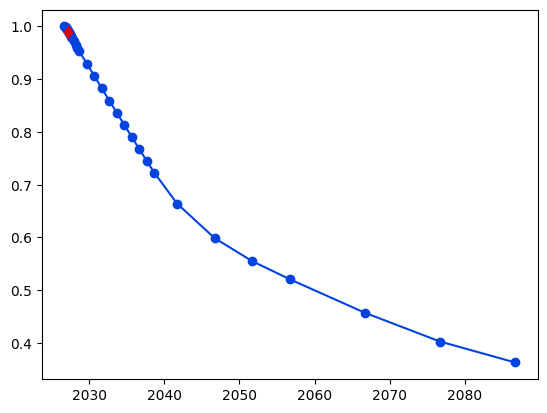
\includegraphics[width=0.7\textwidth]{figures/linear_discount_curve}
	\caption{Plot of the discount curve and of the computed discount factor.}
	\label{fig:linear_discount_curve}
\end{figure}

\section{Forward Rates}
\label{calculating-forward-rates}
A forward rate is an interest rate applicable to a financial transaction that will take place in the future. It can be considered as the market's expectation for future prices and can serve as an indicator of how it believes will perform. Contrary the \emph{spot rate} is used by buyers and sellers looking to make an immediate purchase or sale.

Forward rates are calculated from the spot rate by exploiting the no arbitrage condition which states that investing at rate $r_1$ for the period $(0, T_1)$ and then \emph{re-investing} at rate $r_{1,2}$ for the time period $(T_1, T_2)$ should be equivalent to invest at rate $r_2$ for the full time period $(0, T_2)$. Essentially two investors shouldn't be able to earn money from arbitraging between different interest periods. That said:

\begin{equation}
(1+r_1 T_1)[1+r_{1,2}(T_2 - T_1)] = 1 + r_2 T_2
\label{eq:no_arbitrage_r}
\end{equation}
Solving for $r_{1,2}$ leads to

\begin{equation}
F(T_1, T_2) = r_{1,2} = \frac{1}{T_2 - T_1}\Big(\frac{1+r_2 T_2}{1+r_1 T_1} - 1 \Big)
\label{eq:forward_rate_simple}
\end{equation}
The same expression in terms of discount factors becomes
\begin{equation}
F(T_1, T_2) = \frac{1}{T_2 - T_1}\Big(\frac{D(0, T_1)}{D(0, T_2)} - 1 \Big)
\end{equation}
%Considering continuously compounded rates instead Eq.~\ref{eq:no_arbitrage_r} can be written as
%\begin{equation}
%\begin{gathered}
%e^{r_{2}T_{2}}=e^{r_{1}T_{1}}\cdot \ e^{r_{1,2} (T_{2}-T_{1})}\quad(\textrm{then equating the exponents})\\
%%\textrm{log}\left(e^{r_{2}T_{2}}\right)=\textrm{log}\left(e^{r_{1}T_{1}+ r_{1,2} (T_{2}-T_{1})}\right) \\
%r_{2}T_{2}=r_{1}T_{1}+r_{1,2}(T_{2}-T_{1})\implies r_{1,2} = \cfrac{r_2 T_2 - r_1 T_1}{T_2 - T_1} 
%\end{gathered}
%\end{equation}
%and the corresponding expression for the forward rate is
%\begin{equation}
%F(T_1, T_2) = r_{1,2} = \frac {1}{T_{2}-T_{1}}(\ln D(0,T_{1})-\ln D(0,T_{2}))
%\quad(\textrm{since now } D(0, T_i)=e^{-r_i T_i})
%\label{eq:forward_rate_continous}
%\end{equation}

\begin{finmarkets}
The \texttt{TermStructure} class of the \texttt{finmarkets} module computes forward rates at any arbitrary date, given a set of spot rates. This class is quite similar to \texttt{DiscountCurve}, but its logic has been split into two methods: one to interpolate spot rates, another to actually compute the forward rate.

In order to successfully interpolate the rates, dates need to be converted to numbers by evaluating the number of days since a reference date. Also the interpolation date is checked to avoid extrapolations, if it is outside the known range an exception will be raise and the calculation stopped.
\end{finmarkets}

\pythoncodenon{code/discount_3.py}
\noindent
As an example let's compute

\pythoncodenon{code/discount_4.py}

\begin{ioutput}
F(t1, t2; t0) = 0.09998633879781421
F(t2, t3; t0) = 0.11001369863013699
F(t1, t3; t0) = 0.105
\end{ioutput}

\section{Multi-curve Framework}
\label{sec:financial-crisis}

% aggiungere un pezzettino dell'articolo di Mercurio

Prior to the 2008 financial crisis, inter-bank deposits posed little credit/liquidity issues, inter-bank lending rates (e.g. LIBOR, EURIBOR) were essentially a good proxy for risk free rates. Basis swap spreads were negligible and thereby neglected. 

Looking at the historical series of the EURIBOR (6M) rate versus the EONIA Overnight Indexed Swap (OIS-6M) rate over the time interval 2006-2011 in Fig.~\ref{fig:credit_crunch} it becomes apparent how before August 2007 the two rates display strictly overlapping trends differing of no more than 6 bps.

\begin{figure}[htb]
	\centering
	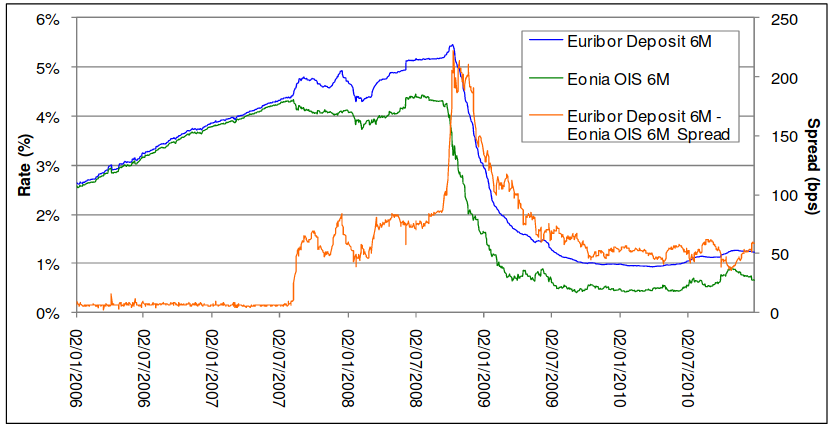
\includegraphics[width=0.9\linewidth]{figures/credit_crunch.png}
	\caption{Historical series of EURIBOR 6M rate versus EONIA OIS 6M rate. The corresponding spread 
		is shown on the right axis (Jan. 06 - Dec. 10 window, source: Bloomberg).}
	\label{fig:credit_crunch}
\end{figure}

A single yield curve constructed out of selected deposit, FRA and swap rates, served both the cash flow projection and discounting purposes.

During the 2008 financial crisis, the failure of some banks however proved that inter-bank lending rates were not risk-free. Meanwhile there was also significant counter-party credit risk arising from derivative transactions that were not subjected to collateral. Basis swap spreads greatly widened, and persist to this day. 

Still looking at Fig.~\ref{fig:credit_crunch} it is clear how in August 2007 a sudden increase of the EURIBOR rate and a simultaneous decrease of the OIS rate led to the explosion of the corresponding basis spread, touching the peak of 222 bps in October 2008, when Lehman Brothers filed for bankruptcy. Successively the basis has sensibly reduced and stabilized between 40 and 60 bps (notice that the pre-crisis level has never been recovered). The same effect is observed for other similar couples of series, e.g. EURIBOR 3M vs OIS 3M.

The existence of such significant basis swap spread reflects the fact that after the crisis interest rate market has been segmented into subareas corresponding to instruments with different underlying rate tenors, characterized by different rate dynamics. 

Traditional single curve based pricing approach ignores these differences. It mixes different underlying rate tenors and incorporates different rate dynamics, eventually leading to inconsistency.
%After the crisis, the market practice has thus evolved to take into account the new market information (e.g. the basis swap spreads, collateralization, etc.), that translate into the additional requirement of homogeneity and funding. The homogeneity requirement means that interest rate derivatives with a given underlying rate tenor must be priced and hedged using vanilla interest rate market instruments with the same underlying. The funding requirement means that the discount rate of any cash flow generated by the derivative must be consistent, by no-arbitrage, with the funding rate associated with that cash flow. 

Driven by the crisis, many derivative contracts have been updated to include permissible credit mitigants for a transaction, such as netting and collateralization in cash. Since standard agreements stipulate daily margination on collateral and the cash collateral earns a return at overnight rate, overnight rate becomes a natural choice for the risk-free discount rate or the funding rate. This is referred to as \emph{OIS discounting}.

Due to the large spread between risk free rate and inter-bank lending rate during and after 2008 financial crisis it is not possible anymore to use a single curve for discounting and derivative valuation. The traditional single curve used for both cash flow projection and discounting turned out to be obsolete. The markets have since nearly switched to \emph{multi-curve framework}. 

For example, if we want to calculate the net present value (NPV) of a forward 6-month EURIBOR coupon, we need to simultaneously use two different discount curves: 

\begin{itemize}
\tightlist
\item the 6-month EURIBOR curve for determining the forward rate;
\item the \euro STR curve for discounting the expected cash flow.
\end{itemize}

%The reason of the abrupt divergence between the Euribor and OIS rates can be explained by considering both the monetary policy decisions adopted by international authorities in response to the financial turmoil, and the impact of the credit crunch on both credit and liquidity risk perception of the market, coupled with the different financial meaning and dynamics of these rates.

%\begin{itemize}
%\tightlist
%\item
%  The Euribor rate is the reference rate for over-the-counter (OTC)
%  transactions in the Euro area. It is defined as the rate at which
%  Euro inter-bank deposits are being offered within the EMU zone by one
%  prime bank to another at 11:00 a.m. Brussels time. The rate fixings
%  for a strip of 15 maturities (from one day to one year) are
%  constructed as the average of the rates submitted (excluding the
%  highest and lowest 15\% tails) by a panel of 42 banks, selected
%  among the EU banks with the highest volume of business in the Euro
%  zone money markets, plus some large international bank from non-EU
%  countries with important euro zone operations. \emph{Thus, Euribor
%  rates reflect the average cost of funding of banks in the inter bank
%  market at each given maturity. During the crisis the solvency and
%  solidity of the whole financial sector was brought into question and
%  the credit and liquidity risk and uremia associated to inter-bank
%  counter-parties sharply increased.} The Euribor rates immediately
%  reflected these dynamics and raise to their highest values over more
%  than 10 years. As seen in the plot above, the Euribor 6M rate suddenly
%  increased on August 2007 and reached 5.49\% on 10th October 2008.
%\item
%  The EONIA rate is the reference rate for overnight OTC transactions in
%  the Euro area. It is constructed as the average rate of the overnight
%  transactions (one day maturity deposits) executed during a given
%  business day by a panel of banks on the inter-bank money market,
%  weighted with the corresponding transaction volumes. \emph{The EONIA
%  Contribution Panel coincides with the Euribor Contribution Panel, thus
%  EONIA rate includes information on the short term (overnight)
%  liquidity expectations of banks in the Euro money market. It is also
%  used by the European Central Bank (ECB) as a method of effecting and
%  observing the transmission of its monetary policy actions. During the
%  crisis the central banks were mainly concerned about stabilizing the
%  level of liquidity in the market, thus they reduced the level of the
%  official rates.} Furthermore, the daily tenor of the EONIA rate makes
%  negligible the credit and liquidity risks reflected on it: for this
%  reason the OIS rates are considered the best proxies available in the
%  market for the risk-free rate.
%\end{itemize}

%Our financial library has to implement the following calculation
%
%\[\mathrm{NPV} = D_{\mathrm{EONIA}}(T_1) \cdot \frac{1}{T_2-T_1}\Big(\frac{D_{\mathrm{LIBOR}}(T_1)}{D_{\mathrm{LIBOR}}(T_2)} - 1 \Big)\]
%\noindent
%In order to do so we can extend the \texttt{DiscountCurve} class with a \texttt{forward\_rate} method
%
%\begin{ipython}
%class DiscountCurve:
%    ...
%    def forward_rate(self, d1, d2):
%        return (self.df(d1) / self.df(d2) - 1.0) * \
%            (365.0 / ((d2 - d1).days))
%\end{ipython}

%As an example let's define \euro STR and EURIBOR curves and compute the net present value of the forward 6-month EURIBOR coupon mentioned before.
%
%\begin{ipython}
%from finmarkets import DiscountCurve, ForwardRateCurve
%from numpy import exp
%from dateutil.relativedelta import relativedelta
%from datetime import date
%
%obs_date = date.today()
%t1 = obs_date + relativedelta(months=3)
%t2 = obs_date + relativedelta(months=9)
%pillar_dates_estr = [obs_date, 
%                     obs_date + relativedelta(months=12),
%                     obs_date + relativedelta(months=34)]
%estr_rates = [1.0, 0.97, 0.72]
%pillar_dates_euribor = [obs_date, 
%                        obs_date + relativedelta(months=5), 
%                        obs_date + relativedelta(months=12)]
%euribor = [0.005, 0.01, 0.015]
%
%estr_curve = DiscountCurve(obs_date, pillar_dates_estr, estr_rates) 
%euribor_curve = ForwardRateCurve(obs_date, pillar_dates_euribor, euribor) 
%
%C = estr_curve.df(t1) * euribor_curve.forward_rate(t1, t2)
%t1_frac, r1 = euribor_curve.interp_rate(t1)
%C_pre2008 = exp(-r1*t1_frac) * euribor_curve.forward_rate(t1, t2)
%
%print (f"C post 2008: {C:.5f} EUR")
%print (f"C pre 2008: {C_pre2008:.5f} EUR")
%\end{ipython}
%\begin{ioutput}
%C post 2008: 0.01513 EUR
%C pre 2008: 0.01522 EUR
%\end{ioutput}

%\subsection{Transitioning away from LIBOR~\cite{bib:str}}
%A working group on euro risk-free rates was established to identify and recommend risk free rates that could serve as a basis for an alternative to current benchmarks used in a variety of financial instruments and contracts in the euro area, such as the euro overnight index average (EONIA) and the euro inter-bank offered rate (EURIBOR). 
%
%The group recommended on September 2018 that the euro short-term rate (\euro STR) be used as the risk-free rate for the euro area and is now focused on supporting the market with transitioning.
%The ECB published the \euro STR for the first time on 2nd October 2019, reflecting trading activity on 1st October 2019.
%
%The working group recommends that market participants should gradually replace EONIA with the \euro STR as a reference rate for all products and contracts and make all necessary adjustments for using the \euro STR as their standard benchmark The working group recommends the \euro STR plus a fixed spread of 8.5
%basis points as the EONIA fallback rate for all products and purposes. The working group recommends that market participants should: consider, whenever feasible and appropriate, no longer entering into new contracts referencing EONIA, in particular new contracts maturing after 31 December 2021, as EONIA will cease to exist after that date.
%
%%The working group is also looking at identifying fallbacks for
%%EURIBOR based on the STR. Both backward and forward-looking
%%options are being considered. As part of its work on forward-looking
%%options, in March 2019 the working group recommended a
%%methodology based on (tradable) overnight index swap (OIS) quotes
%%for calculating a STR-based forward-looking term structure and later
%%invited benchmark administrators to express their interest in
%%producing such a term structure.

\section*{Exercises}
\cprotEnv\begin{question}
Mario wants to lease a car for 3 years. The car dealer has given him two payment options to choose from:
\begin{table}[htbp]	
    \centering	
	\begin{tabular}{l|c|c|c|c|c|c|c}
		Year & 0 & 0.5 & 1 & 1.5 & 2 & 2.5 & 3 \\
		\hline
		Option 1 &	3000	& 500 & 500 &	500 & 500 & 500 & 500 \\
		\hline
		Option 2 &	5000	& 350 & 350 &	350 & 350 & 350 & 350 \\
	\end{tabular}
\end{table}

\noindent
Which payment option should he choose? (Assume an annual discount rate of 10\%)
\end{question}

\cprotEnv\begin{solution}
In order to decide which payment to choose from, he would need to calculate the PV of the payment stream, and look at which costs him the least. 
	
\begin{gather*}
DF_n = 1/(1 + r)^n \\
PV_n = [\textrm{payment in year n}] / DF_n \\
Total PV = \sum PV_n
\end{gather*}
	
\begin{ipython}
def discount_factor(year):
	return 1/(1 + 0.1)**year
		
opt1 = {0:3000, 0.5:500, 1:500, 1.5:500, 2:500, 2.5:500, 3:500}
opt2 = {0:5000, 0.5:350, 1:350, 1.5:350, 2:350, 2.5:350, 3:350}
		
npv1 = sum([discount_factor(k)*v for k,v in opt1.items()])
npv2 = sum([discount_factor(k)*v for k,v in opt2.items()])
		
print (f"Option1: {npv1:.1f}")
print (f"Option2: {npv2:.1f}")
\end{ipython}
\begin{ioutput}
Option1: 5547.5
Option2: 6783.3
\end{ioutput}
Hence he should choose option 1 as it costs him less than option 2.
\end{solution}

\begin{question}
Tots and Toys, Inc. offers Maria an investment plan that requires 10 yearly payments of 1000 USD, starting from today. The plan promises an annual return of 8\% on her investment. The money will be available to her at the end of 10 years (no withdrawals are allowed before that time.) 
What amount will she get at the end of 10 years?
\end{question}

\cprotEnv\begin{solution}
The question requires you to find the future value (FV) of the stream of payments. The rate given is 8\%. In order to find the FV, you need to multiply each amount by its respective FV factor, and then sum the results.
	
\begin{ipython}
def fv_factor(year):
    return (1 + 0.08)**year
		
fv = 0
for year in range(11):
    fv += 1000*fv_factor(year)
		
print (f"future value: {fv:.1f}")
\end{ipython}
\begin{ioutput}
future value: 16645.5 USD
\end{ioutput}
\end{solution}

\cprotEnv\begin{question}
\label{ex:yield_discount}
Build a curve with the given inputs (pillar dates and yields), \href{https://raw.githubusercontent.com/matteosan1/finance_course/develop/input_files/exercise_8.43.csv}{exercise\_8.43.csv}.
By interpolation, find the 18M yield, then draw the yield curve, draw the curve and discount factors at the following dates
\begin{ipython}
df_dates = [date(2025, 4, 15), date(2031, 4, 15)]
\end{ipython}
\end{question}

\cprotEnv\begin{solution}
To interpolate the given yields the \texttt{interp1d} function can be used. Before doing that it is necessary to convert the dates into numbers (i.e. the difference between the actual date and "today").
\begin{ipython}
import pandas as pd
from scipy.interpolate import interp1d
from datetime import date
from dateutil.relativedelta import relativedelta

df = pd.read_csv("exercise_8.43.csv")
print (df.head())

obs_date = date.today()

df_dates = [obs_date + relativedelta(months=66),
            obs_date + relativedelta(months=126)]

num_dates = [d.toordinal() for d in df['dates']]
interpolator = interp1d(num_dates, df['yields'])
target = (obs_date + relativedelta(months=18)).toordinal()
print (interpolator(target)
\end{ipython}
\begin{ioutput}
-0.8077935491803279
\end{ioutput}

Figure~\ref{fig:ex_yield} shows the yield curve and the interpolated point of the 18m yield.

\begin{figure}[htpb]
\centering
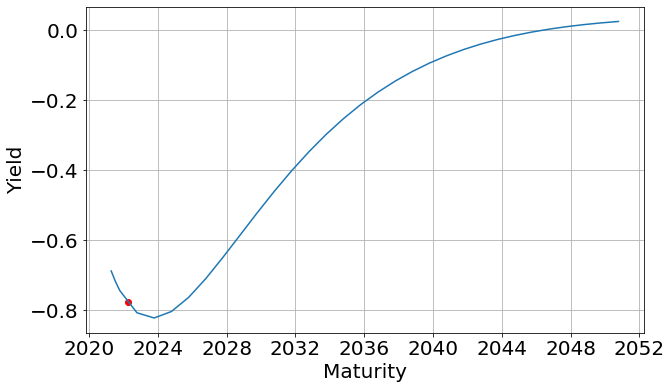
\includegraphics[width=0.7\linewidth]{figures/ex_yield}
\caption{Yield curve resulting from the exercise inputs.}
\label{fig:ex_yield}
\end{figure}

To construct the discount curve first it is necessary to define the discount factors from the yields. Then you need to instantiate a \texttt{DiscountCurve} object with the mandatory inputs and call the \texttt{df} method to compute the discount factors at the required dates.
\begin{ipython}
from finmarkets import DiscountCurve

dfs = []
dates = [d.date() for d in pd.to_datetime(df['dates'])]
for i, d in enumerate(dates):
    dfs.append(np.exp(-df['yields'][i]/100*((d-obs_date).days/365)))
dc = DiscountCurve(obs_date, dates[1:], dfs[1:])
print (dc.df(df_dates[0]))
print (dc.df(df_dates[1]))
\end{ipython}develop
\begin{ioutput}
1.0334049958222
1.0329281686679732
\end{ioutput}
\noindent
Figure~\ref{fig:ex_discount} shows the discount curve and the interpolated discount factors.

\begin{figure}[htpb]
\centering
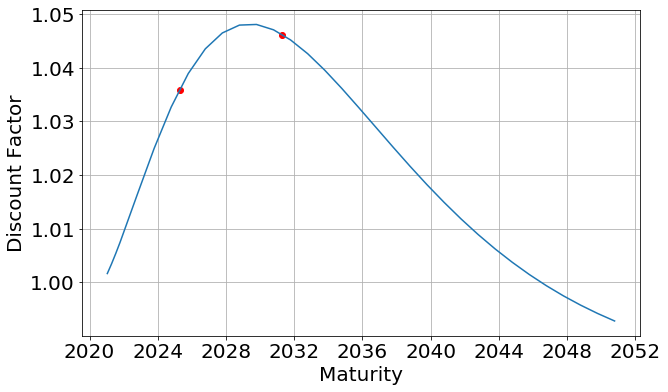
\includegraphics[width=0.7\linewidth]{figures/ex_discount}
\caption{Discount curve resulting from the exercise inputs.}
\label{fig:ex_discount}
\end{figure}
\end{solution}

%\cprotEnv\begin{question}
%Calculate the forward interest for the period from six months (180/360) from now to nine months (270/360) from now if the six month rate is 4.50\% p.a. and the nine month rate is 4.25\% p.a.
%\end{question}
%
%\cprotEnv\begin{solution}
%FV
%FV
%6
%9
%1 +0.045* 180/360 1025
%1 +0.0425 *270-360 10525
%
%360/90 *1.03188/1.02250 = 0.0367 = 3.67
%\end{solution}


\begin{question}
Given the same inputs of Exercise~\ref{ex:yield_discount} and using the \texttt{termStructure} class compute the 10y forward rate in 1y from today. 
\end{question}

\cprotEnv\begin{solution}
\begin{ipython}
import pandas as pd
from finmarkets import ForwardRateCurve

from datetime import date
from dateutil.relativedelta import relativedelta

df = pd.read_csv("exercise_8.43.csv")
obs_date = date.today()

dates = [d.date() for d in pd.to_datetime(df['dates'])]
fc = ForwardRateCurve(obs_date, dates, df['yields'])
print (f"{fc.forward_rate(obs_date + relativedelta(years=1):.4f}%")
\end{ipython}
\begin{ioutput}
-0.0023%
\end{ioutput}
\end{solution}

%\begin{question}
%Copy into the file \texttt{finmarkets.py} the function used to compute Black Scholes formula used in Ex.~\ref{ex:BS2}. This is another utility for our financial library. Then repeat Ex.~\ref{ex:BS2} now using the version of the Black and Scholes formula in the \texttt{finmarkets} module.
%\end{question}
%
%\begin{solution}
%\begin{tcolorbox}[size=fbox, boxrule=1pt, colback=cellbackground, colframe=cellborder]
%\begin{Verbatim}[commandchars=\\\{\}]
%\PY{k}{import} \PY{n}{finmarkets}
%        
%\PY{n}{s} \PY{o}{=} \PY{l+m+mi}{800}
%\PY{c+c1}{\PYZsh{} strikes expressed as \PYZpc{} of spot price}
%\PY{n}{moneyness} \PY{o}{=} \PY{p}{[} \PY{l+m+mf}{0.5}\PY{p}{,} \PY{l+m+mf}{0.75}\PY{p}{,} \PY{l+m+mf}{0.825}\PY{p}{,} \PYZbs{}
%             \PY{l+m+mf}{1.0}\PY{p}{,} \PY{l+m+mf}{1.125}\PY{p}{,} \PY{l+m+mf}{1.25}\PY{p}{,} \PY{l+m+mf}{1.5} \PY{p}{]}
%\PY{n}{vol} \PY{o}{=} \PY{l+m+mf}{0.3}
%\PY{n}{ttm} \PY{o}{=} \PY{l+m+mf}{0.75}
%\PY{n}{r} \PY{o}{=} \PY{l+m+mf}{0.005}
%
%\PY{n}{result} \PY{o}{=} \PY{p}{\PYZob{}}\PY{p}{\PYZcb{}}
%\PY{k}{for} \PY{n}{m} \PY{o+ow}{in} \PY{n}{moneyness}\PY{p}{:}
%    \PY{n}{result}\PY{p}{[}\PY{n}{s}\PY{o}{*}\PY{n}{m}\PY{p}{]} \PY{o}{=} \PY{n}{finmarkets.call}\PY{p}{(}\PY{n}{s}\PY{p}{,} \PY{n}{m}\PY{o}{*}\PY{n}{s}\PY{p}{,} \PY{n}{r}\PY{p}{,} \PY{n}{vol}\PY{p}{,} \PY{n}{ttm}\PY{p}{)}
%\PY{n}{result}
%
%\{400.0: 401.66074527896365,
%  600.0: 213.9883852521275,
%  660.0: 166.85957363897393,
%  800.0: 84.03697017660357,
%  900.0: 47.61880394696229,
%  1000.0: 25.632722952585738,
%  1200.0: 6.655275227771156\}
%\end{Verbatim}
%\end{tcolorbox}
%\end{solution}


 
\chapter{Bonds}
\label{bonds}

A bond is an instrument that represents a loan made by an investor to a borrower (typically corporate or governmental). Bonds are used by companies, municipalities, states, and sovereign governments to finance projects and operations. 

Owners of bonds are debt-holders, or creditors of the issuer. Bond details include the principal (the loan amount), the end date (when the loan principal is due to be paid to the bond owner) and usually includes the terms for variable or fixed interest payments made by the borrower.

The \emph{coupon} is the interest rate that the issuer pays to the holder. This rate can be fixed throughout the life of the bond but it can also vary with a money market index, such as LIBOR, or it can be even more exotic.

\section{Valuing a Bond}
\label{sec:bond_pricing}

The value of a bond can be computed as the present discounted value of future cash-flows generated by the bond itself.

For example consider a 3-years bond with a face value of \euro{100} providing coupons at a 6\% rate annually. Assume also that the discount rates are 5.0\% 5.8\% and 6.4\% for 1, 2, 3 years. The value will be then:

\begin{equation*}
P_{\mathrm{bond}}=6e^{-0.05\cdot 1}+6e^{-0.058\cdot 2}+106e^{-0.064\cdot 3}
\end{equation*}

\begin{ipython}
from numpy import exp

rates = {1:0.05, 2:0.058, 3:0.064}
N = 100
maturity = 3
fixed_coupon = 0.06
price = 0

for tau in range(1, maturity+1):
    price += N * fixed_coupon * exp(-rates[tau] * (tau))
price += N * exp(-rates[tau] * (tau))

print (f"{price:.2f} EUR")
\end{ipython}
\begin{ioutput}
98.53 EUR
\end{ioutput}

\subsection{Yield to Maturity}
The \emph{yield to maturity} is the interest rate that makes the present value of the future coupon payments equal to the current bond price, that is, for a known price $P_0$, the yield is the solution $y$ to the equation

\begin{equation}
P = \sum_{t=1}^T e^{-yt}C + e^{-yT}N 
\label{eq:yield_to_maturity}
\end{equation}
where $C$ is the coupon end $N$ the nominal.

Finding the yield to maturity is equivalent to find the zeros of Eq.~\ref{eq:yield_to_maturity}.
To find the zeros of a function $f(x)$ means to determine the values $\hat{x}$ such that $f(\hat{x})=0$ and the process is equivalently called finding the roots of $f(x)$. There are various methods to achieve that, in the following we will see two of them.
\label{sec:root_finding}
\emph{Bisection}~\cite{bib:bisection} method is considered the simplest one-dimensional root-finding algorithm.
Suppose we know two points of an interval $[a,b]$, and that $f(a)< 0$ and $f(b)> 0$.
Since the value of $f(a)$ is negative and $f(b)$ is positive, the bisection method assumes that the root $x$ lies somewhere between $a$ and $b$.

Taking the midpoint of this $[a, b]$ interval as $c$, the algorithm evaluates the value $f(c)$.
If $f(c) = 0$ or is very close to zero by some predetermined error tolerance value, then a root is declared as found. If $f(c)< 0$, then we may conclude that a root exists along the interval $[c, b]$, or along $[a,c]$ otherwise.

On the next evaluation, $c$ is replaced as either $a$ or $b$ accordingly. With the new interval shortened, the bisection method repeats with the same evaluation to determine the next value of $c$. This process continues, shrinking the width of the interval until the root is determined as found. Figure~\ref{fig:bisection} shows an example of bisection algorithm application.

\begin{figure}[htbp]
\centering
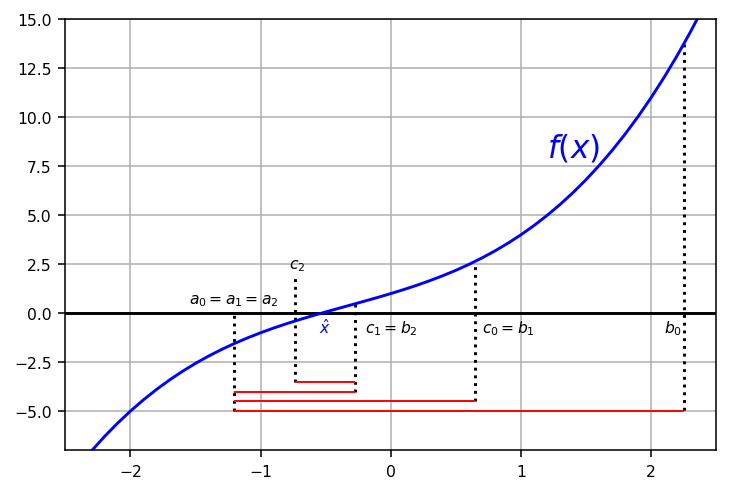
\includegraphics[width=0.7\linewidth]{figures/bisection}
\caption{Example of bisection algorithm to find the roots of a function $f(x)$.}
\label{fig:bisection}
\end{figure}

The biggest advantage of the bisection method is it is guaranteed to converge to an approximation of the root, given a predetermined error tolerance level and the maximum number of iterations allowed. It should be noted that the bisection method does not require knowledge of the derivative of the unknown function. In certain continuous functions, the derivative could be complex or even impossible to calculate. This makes this method extremely valuable for working on functions that are not smooth.
Contrary, its major drawback is that it takes up more computational time in the iterative evaluation as compared to other root-finder methods. 

Although this method is simple enough to be quickly implemented in \texttt{python} we will opt for the surely bug free version available as \texttt{scipy.optimize.bisect} (for the usage of \texttt{args} see Section~\ref{sec:kwargs_args}).

\begin{ipython}
from scipy.optimize import bisect 

def ytom(y, N, C, P0, maturity_years, tenor=1): 
	price = 0
	for p in range(1, int((maturity_years/tenor)+1)):
		price += C*tenor*N/(1+y*tenor)**p
	price += N/(1+y*tenor)**p - P0 
	return price

print (bisect(ytom, -0.3, 1, args=(100, 0.05, 95, 6, 0.5)))
\end{ipython}
\begin{ioutput}
0.060047636994841024
\end{ioutput}

%%%% NEWTON-RAPHSON
An alternative algorithm is the \emph{Brent's method}~\cite{bib:brent} which combines the advantages of both bisection and secant (another root-finding algorithm) methods. Its \texttt{python} implementation is \texttt{scipy.optimize.brentq}.

\begin{ipython}
from scipy.optimize import brentq
    
print (brentq(ytom, -0.3, 1, args=(100, 0.05, 95, 6, 0.5)))
\end{ipython}
\begin{ioutput}
0.06004763699594817
\end{ioutput}

\noindent
The results match down to the eleventh digit.

\subsection{Duration}
The duration of a bond is the \emph{weighted average maturity} of the bond

\begin{equation}
\textrm{duration} = \sum_{i=1}^{n} t_i \left[\cfrac{C_i D_i}{P}\right] 
\end{equation}
where $C_i$ is the cash-flow in period $t_i$, $D_i$ is the corresponding discount factor and $P$ is the bond price.
Knowing the bond yield from Eq.~\ref{eq:yield_to_maturity} the previous equation becomes:
\begin{equation}
\textrm{duration} = \sum_{i=1}^{n} t_i \left[\cfrac{C_i e^{-yt_i}}{P}\right] 
\label{eq:duration}
\end{equation}

This quantity is sometimes referred to as \emph{Macaulay Duration}. By accounting for the present value of future bond payments, the Macaulay duration helps an investor to evaluate and compare bonds independent of their time to maturity.
It estimates how many years it will take for an investor to be repaid the bond’s price by its total cash-flows.

Imagine a three-year bond with a face value of \$100 that pays a 10\% coupon semi-annually and has a yield to maturity (YTM) of 6\%. We will first compute the present value of the bond and then calculate its Macaulay duration.

\begin{ipython}
def bond_pv(N, C, r, maturity, tenor=1):
	price = 0
	for tau in range(1, int((maturity/tenor)+1)):
		price += N * C*tenor / (1+r*tenor)**(tau)
	price += N / (1+r*tenor)**(tau)
	return price

def mac_duration(N, C, y, maturity, P0, tenor=1): 
	d=0
	for tau in range(1, int((maturity/tenor)+1)):
		d += tau*N*C*tenor/(1+y*tenor)**tau/P0
	d += tau*N/(1+y*tenor)**tau/P0 
	return d

P0 = bond_pv(100, 0.1, 0.06, 3, 0.5)
print (f"Bond price: {P0:.2f}")

dur = (mac_duration(100, 0.1, 0.06, 3, P0, 0.5))
print (f"Duration: {dur:.2f}")
\end{ipython}
\begin{ioutput}
Bond price: 110.83
Duration: 5.37
\end{ioutput}

This result can be interpreted by saying that it will take about two years and 7 months to be repaid for the bond expenses.

Equation~\ref{eq:duration} connects the bond price to the yield through duration. When a small change in yield $\Delta y$ happens
\begin{equation}
\Delta P = \cfrac{dP}{dy}\Delta y
\label{eq:price_1st_order}
\end{equation}
\noindent
Computing the derivative of the bond price from Eq.~\ref{eq:yield_to_maturity} we get

\begin{equation}
\Delta P = -\Delta y\sum_i C_i t_i e^{-yt_i}
\label{eq:price_yield}
\end{equation}
\noindent
which indicates there is a negative relationship between $P$ and $y$ (i.e. when bond yield increases the bond price decrease). 

Substituting Eq.~\ref{eq:duration} into Eq.~\ref{eq:price_yield} 
\begin{equation}
\Delta P = -PD\Delta y \quad\rightarrow\quad \cfrac{\Delta P}{P} = -D\Delta y
\label{eq:price_sens}
\end{equation}

This is an approximate relationship between percentage changes in a bond price and changes in its yield.

Consider a 3-year 10\% coupon bond with a face value of 100\$. Suppouse its yield is 12\% and that coupon payments of 5\$ are made every 6 months. Using the previous functions it is possible to compute bond price and duration

\begin{ipython}
price = bond_pv(100, 0.1, 0.12, 3, 0.5)
print (f"Price: {price:.3f}")

dur = mac_duration(100, 0.1, 0.12, 3, price, 0.5)
print (f"Duration: {dur:.3f}")
\end{ipython}
\begin{ioutput}
Price: 95.083
Duration: 5.310
\end{ioutput}

Replacing those values into Eq.~\ref{eq:price_sens} it is possible to estimate the sensitivity of the bond price to small changes of the yield.
Assuming for example an yield variation of 10 basis points
\begin{ipython}
dP = -price*dur*0.001
print (f"DeltaP: {dP:.3f}")
print (f"P+DP: {price+dP:.3f}")
\end{ipython}
\begin{ioutput}
DeltaP: -0.505
P+DP: 94.578
\end{ioutput}

To check how good is this approximation we can compute the bond price assuming the new yield
\begin{ipython}
today = date.today()

price = bond_pv(100, 0.1, 0.121, 3, 0.5)
print (f"Price: {price:.3f}")
\end{ipython}
\begin{ioutput}
Price: 94.845
\end{ioutput}

Which is in good agreement with the approximate calculation.
When the yield variation is larger the simple linear approximation is not valid anymore as shown in Fig.~\ref{fig:bond_sensitivity}.

\begin{figure}[htbp]
\centering
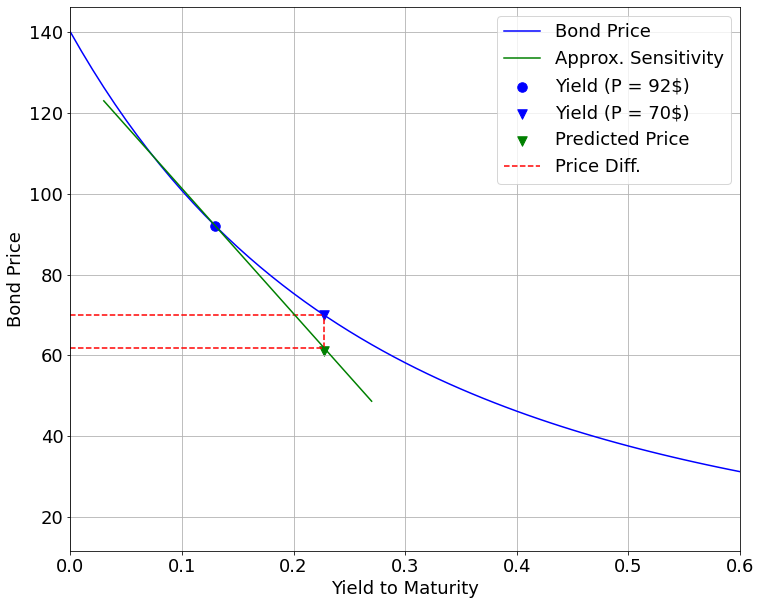
\includegraphics[width=0.7\linewidth]{figures/bond_duration}
\caption{Bond price sensitivity to yield variation. For large movements of the yield the simple linear approximation given by
 Eq.~\ref{eq:price_sens} is not valid anymore.}
\label{fig:bond_sensitivity}
\end{figure}

\subsection{Price Value of a Basis Point}
A very common risk measure is the sensitivity of the price of a bond to changes in its yield. The price value of a basis point, PVBP, also called the dollar value of a basis point or $DV01$, measures the decline in price associated with a one basis point increase in the yield.

\begin{equation}
DV01 = -\cfrac{dP}{dy}\times 0.0001
\end{equation}

$DV01$ can be computed directly, by computing the price at the current yield, adding one basis point to the yield, and recomputing the price.

$DV01$ can also be computed directly from duration. In particular, we have seen that $dP/P = -D dy$. Hence $dP = -D Pdy$ and

\begin{equation}
DV01 = -D P \times 0.0001
\end{equation}

\subsubsection{Modified Duration}
In the previous analysis we have assumed continuous compounding. If instead $y$ is expressed with a compounding frequency of $m$ times per year then 
\begin{equation}
\Delta P = \cfrac{PD\Delta y}{1+y/m}
\end{equation}
\noindent
The quantity $D^{*}$, defined by
\begin{equation}
D^{*} = \cfrac{D}{1+y/m}
\end{equation}
\noindent
is referred to as \emph{modified duration}. 

\subsection{Convexity}
The duration relationship studied in the previous Section is valid only for small changes in yields. Since Eq.~\ref{eq:price_1st_order} is just a Taylor expansion to first order, to improve its accuracy we need to go to higher orders

\begin{equation}
\Delta P = \cfrac{dP}{dy}\Delta y + \cfrac{1}{2} \cfrac{d^2 P}{dy^2}\Delta y^2 = -D\Delta y + \cfrac{1}{2} \textrm{Conv} \Delta y^2 
\end{equation}
\noindent
The quantity $\textrm{Conv} = \frac{\sum_i C_i t_i^2 e^{-yt_i}}{P}$ is called \emph{convexity} and parametrizes the behaviour of the bond price for large yield variations.

Considering a portfolio of bonds, the convexity tends to be greatest when it provides payments evenly over a long period of time. Contrary it is least when the payments are concentrated around a particular point in time. 

Choosing a portfolio of assets with net duration and net convexity both close to zero, we make ourselves immune to relatively large shifts in the zero curve (i.e. large movements of the yield).

\subsection{Duration, Convecxity and DV01 of a Bond Portfolio}
The duration of a bond portfolio, $D_p$, is computed as the weighted average of the durations of the individual
bonds:
\begin{equation}
D_p = \sum_{i=1}^{K} \alpha_i D_i
\end{equation}
where $K$ is the number of different bonds and $\alpha_i$ is the fraction of portfolio dollars invested in bond $i$. Similarly, the convexity of a bond portfolio, Conv$_p$, is the weighted average of the convexities of the individual bonds.
\begin{equation}
\textrm{Conv}_p = \sum^{K}_{i=1} \alpha_i \textrm{Conv}_i
\end{equation}
The $DV01_p$ of a portfolio is defined as the change in value resulting from equal one basis point declines in all yields. Let $DV01_i$ represent the dollar value of a basis point associated with the i$^{th}$ bond. Then
\begin{equation}
DV01_p = \sum^{K}_{i=1}x_i DV01_i
\end{equation}
where $x_i$ is the number of bonds of type $i$ in the portfolio.

\section*{Exercises}
\begin{question}
A Treasury bond has a coupon of 9\%, a face value of 1000 USD and matures 10 years from today. For a treasury bond the interest on the bond is paid in semi-annual coupons. The current risk-less interest rate is 12\% (compounded semi-annually).
\begin{enumerate}
\item Suppose you purchase the Treasury bond described above and immediately thereafter the risk-less interest rate falls to 8\%. (compounded semi-annually). What would be the new market price of the bond?
\item What is your best estimate of what the price would be if the risk-less interest rate was 9\% (compounded semi-annually) ?
\end{enumerate}
\end{question}

\cprotEnv\begin{solution}
\begin{ipython}
import numpy as np

N = 1000
maturity = 10
coupon = 0.09
tenor = 0.5
rates = {i:0.08 for i in range(1, int((maturity/tenor)+1))}

price = 0
for tau in range(1, int((maturity/tenor)+1)):
    price += N * coupon*tenor / (1+rates[tau]*tenor)**(tau)
price += N / (1+rates[tau]*tenor)**(tau) 

print (f"{price:.2f} USD")
\end{ipython}
\begin{ioutput}
1067.95 USD
\end{ioutput}

\begin{ipython}
rates = {i:0.09 for i in range(1, int((maturity/tenor)+1))}
	
price = 0
for tau in range(1, int((maturity/tenor)+1)):
    price += N * coupon*tenor / (1+rates[tau]*tenor)**(tau)
price += N / (1+rates[tau]*tenor)**(tau) 
	
print (f"{price:.2f} USD")
\end{ipython}
\begin{ioutput}
1000.00 USD
\end{ioutput}
\end{solution}

\begin{question}
A 100 USD, 10 year bond was issued 7 years ago at a 10\% annual interest rate. The current interest rate is 9\%.The current price of the bond is 100.917 USD. Use annual, discrete compounding. Calculate the bonds yield to maturity.
\end{question}

\cprotEnv\begin{solution}
\begin{ipython}
from scipy.optimize import brentq

def ytom(y, N, C, P0, maturity_years, tenor=1): 
    price = 0
    for p in range(1, int((maturity_years/tenor)+1)):
        price += C*tenor*N/(1+y*tenor)**p
    price += N/(1+y*tenor)**p - P0 
    return price

y = brentq(ytom, -0.3, 1, args=(100, 0.10, 100.917, 3, 1))
print (f"yield to maturity: {y:3f}")
\end{ipython}
\begin{ioutput}
yield to maturity: 0.096
\end{ioutput}    
\end{solution}

\begin{question}
Suppose you are trying to determine the interest rate sensitivity of two bonds. Bond 1 is a 12\% coupon bond with a 7-year maturity and a 1000 USD principal. Bond 2 is a ‘zero-coupon’ bond that pays 1120 USD after 7 year.The current interest rate is 12\%.
\begin{enumerate}
\item Determine the duration of each bond.
\item If the interest rate increases 100 basis points (100 basis points = 1\%), what will be the capital loss on each bond ?
\end{enumerate}
\end{question}

\cprotEnv\begin{solution}
The first part of the exercise can be solved by applying the definition of duration.
\begin{ipython}
def zero_bond_pv(N, r, maturity):
    return N / (1+r)**(maturity)

def zero_mac_duration(P0, maturity): 
    return maturity * P0/P0 

def bond_pv(N, C, r, maturity, tenor=1):
    price = 0
    for tau in range(1, int((maturity/tenor)+1)):
        price += N * C*tenor / (1+r*tenor)**(tau)
    price += N / (1+r*tenor)**(tau)
    return price

def mac_duration(N, C, y, maturity, tenor=1): 
    P0 = bond_pv(N, C, y, maturity, tenor)
    d=0
    for tau in range(1, int((maturity/tenor)+1)):
        d += tau*N*C*tenor/(1+y*tenor)**tau/P0
    d += tau*N/(1+y*tenor)**tau/P0 
    return P0, d

P0, dur = mac_duration(1000, 0.12, 0.12, 7)
print (f"Bond price: {P0:.2f}")
print ("Duration: {dur:.2f}")

PZ = zero_bond_pv(1120, 0.12, 7) 
print (f"Zero Bond price: {PZ:.2f} USD")
durZ = zero_mac_duration(PZ, 7)
print (f"Zero Duration: {durZ:.2f}")
\end{ipython}
\begin{ioutput}
Bond price: 1000.00
Duration: 5.11
Zero Bond price: 506.63
Zero Duration: 7.00
\end{ioutput}

For the second part the exact capital losses can be obtained by re-computing the bond prices with the new rate.

\begin{ipython}
P1 = bond_pv(1000, 0.12, 0.13, 7)
print (f"Bond price: {P1:.2f} USD")
print (f"Capital loss Bond: {100*(P1-P0)/P0:.3f}%")

PZ1 = zero_bond_pv(1120, 0.13, 7) 
print (f"Bond price: {PZ1:.2f} USD".format(PZ1))
print (f"Capital loss Zero Bond: {100*(PZ1-PZ)/PZ:.3f}%")
\end{ipython}
\begin{ioutput}
Bond price: 955.77 USD
Capital loss Bond: -4.423%
Bond price: 476.07 USD
Capital loss Zero Bond: -6.033%
\end{ioutput}

An approximate solution instead can be estimated by applying the relation $\Delta P/P = -D\Delta r$.
\begin{ipython}
closs1 = -dur*0.01
print (f"Capital loss1: {closs1*100:.3f}%")

closs2 = -durZ*0.01
print (f"Capital loss1: {closs2*100:.3f}%")
\end{ipython}
\begin{ioutput}
Capital loss1: -5.111%
Capital loss1: -7.000%
\end{ioutput}
\end{solution}

%\begin{question}
%From the \texttt{OvernightIndexSwap} created in the previous example derive a discount curve using the bootstrap method.
%\end{question}
%
%\cprotEnv\begin{solution}
%We have just created some swaps from the market quotes in the previous exercise, so now we can just create a list with the pillar dates.
%
%\begin{ipython}
%observation_date = date(2019, 10, 23)
%pillar_dates = [observation_date]
%
%for swap in swaps:
%    pillar_dates.append(swap.payment_dates[-1])
%
%# this shouldn't be necessary if the original
%# list of market quotes is sorted
%pillar_dates = sorted(pillar_dates)
%\end{ipython}
%Define the objective function: the sum of the squared NPVs of the OIS.
%\begin{ipython}
%def objective_function(x):
%    curve = DiscountCurve(observation_date,
%        pillar_dates, x)
%
%    sum_sq = 0.0
%    for swap in swaps:
%        sum_sq += swap.npv(curve) ** 2
%    return sum_sq
%\end{ipython}
%Set the initial value of the discount factors (\(x_i\)) to 1 with a range of variability \([ 0.01, 10]\), in addition the first element of the list, today's discount factor, will be fixed to 1 (variability \([1, 1]\)).
%
%\begin{ipython}
%x0 = [1.0 for i in range(len(pillar_dates))]
%
%bounds = [(0.01, 10.0) for i in range(len(pillar_dates))]
%bounds[0] = (1.0, 1.0)
%\end{ipython}
%Finally launch the minimizer to find the discount factors (\(\mathbf{x}\)).
%
%\begin{ipython}
%from scipy.optimize import minimize
%
%result = minimize(objective_function, x0, bounds=bounds)
%print (result)
%\end{ipython}
%\begin{ioutput}
%     fun: 0.000819919032900304
%hess_inv: <34x34 LbfgsInvHessProduct with dtype=float64>
%     jac: array([ 6.58948735e+05, -1.58720803e+01, -6.53143264e+01, 
%                 -1.03323232e+02, -1.26050260e+02, -1.31748898e+02, 
%                 -1.20374599e+02, -9.15399651e+01, -4.24363322e+01,  
%                  2.44903182e+01,  1.14345243e+02,  2.22002243e+02,
%                 -3.72021700e+00,  4.21398633e+01,  4.21787852e+01,  
%                  4.22369487e+01,  4.23327026e+01,  4.31814758e+01,  
%                  4.44924460e+01,  4.62078978e+01,  4.82906823e+01, 
%                  -3.69972738e+00,-1.42454702e+00,  7.53771932e-01,
%                  2.79741018e+00,  4.62896699e+00,  6.24844054e+00,  
%                  9.93101553e+00,  1.31122434e+01,  1.42880909e+01,  
%                  1.48279215e+01,  1.50787019e+01,  1.43267935e+01,  
%                  1.38451324e+01])
% message: b'CONVERGENCE: REL\_REDUCTION\_OF\_F\_<=\_FACTR*EPSMCH'
%    nfev: 840
%     nit: 7
%  status: 0
% success: True
%       x: array([1.        , 1.00030147, 1.00058831, 1.00089012, 1.00119726,
%                 1.00147996, 1.00178743, 1.00208107, 1.00238467, 1.00267865,
%                 1.00298261, 1.00327737, 1.00357104, 1.00357104, 1.00355063,
%                 1.00352002, 1.00346901, 1.00302007, 1.00232627, 1.00141821,
%                 1.00031629, 0.99911234, 0.99790839, 0.99675545, 0.99567393,
%                 0.99470465, 0.9938476 , 0.99189884, 0.99021534, 0.98959296,
%                 0.98930728, 0.98917464, 0.98957256, 0.98982763])
%\end{ioutput}
%\end{solution}
%
%\begin{question}
%Consider the bearing coupon bonds listed in the next Table. Using the pseudo-inverse method determine discount factors and yields (assume continuous compounding).
%
%\begin{table}[htb]
%	\begin{center}
%		\begin{tabular}{|c|c|c|}
%			\hline
%			\textbf{price} & \textbf{maturity} & \textbf{coupon} \\
%			\hline
%			\euro{96.60} & 1 & 2.0\% \\
%			\hline
%			\euro{93.71} & 2 & 2.5\% \\
%			\hline
%			\euro{91.56} & 3 & 3.0\% \\
%			\hline
%			\euro{90.24} & 4 & 3.5\% \\
%			\hline
%			\euro{89.74} & 5 & 4.0\% \\
%			\hline
%			\euro{90.04} & 6 & 4.5\% \\
%			\hline
%			\euro{91.09} & 7 & 5.0\% \\
%			\hline
% 			\euro{92.82} & 8 & 5.5\% \\
%			\hline
%			\euro{95.19} & 9 & 6.0\% \\
%			\hline
%			\euro{98.14} & 10 & 6.5\% \\
%			\hline
%		\end{tabular}
%	\end{center}
%\end{table}
%	
%\end{question}
%
%\cprotEnv\begin{solution}
%\begin{ipython}
%import numpy as np
%
%C = np.array([[102, 0, 0, 0, 0, 0, 0, 0, 0, 0],
%              [2.5, 102.5, 0, 0, 0, 0, 0, 0, 0, 0],
%              [3, 3, 103, 0, 0, 0, 0, 0, 0, 0],
%              [3.5, 3.5, 3.5, 103.5, 0, 0, 0, 0, 0, 0],
%              [4, 4, 4, 4, 104, 0, 0, 0, 0, 0],
%              [4.5, 4.5, 4.5, 4.5, 4.5, 104.5, 0, 0, 0, 0],
%              [5, 5, 5, 5, 5, 5, 105, 0, 0, 0],
%              [5.5, 5.5, 5.5, 5.5, 5.5, 5.5, 5.5, 105.5, 0, 0],
%              [6, 6, 6, 6, 6, 6, 6, 6, 106, 0],
%              [6.5, 6.5, 6.5, 6.5, 6.5, 6.5, 6.5, 6.5, 6.5, 106.5]])
%
%P = np.array([96.60, 93.71, 91.56, 90.24, 89.74, 
%              90.04, 91.09, 92.82, 95.19, 98.14])
%
%Cinv = np.linalg.pinv(C)
%d = Cinv.dot(P.T)
%print (d)
%\end{ipython}
%\begin{ioutput}
%[0.94705882 0.89114491 0.83539212 0.7814726  0.72999737 0.68140865
% 0.63578693 0.59296268 0.55300618 0.51574181]
%\end{ioutput}
%
%\begin{ipython}
%from math import log
%
%for i in range(10):
%    print ("yield y{}: {:.3f}%".format(i+1, -log(d[i])/(i+1)*100))
%\end{ipython}
%\begin{ioutput}
%yield y1: 5.439%
%yield y2: 5.762%
%yield y3: 5.995%
%yield y4: 6.164%
%yield y5: 6.294%
%yield y6: 6.393%
%yield y7: 6.470%
%yield y8: 6.533%
%yield y9: 6.582%
%yield y10: 6.621%
%\end{ioutput}
%\end{solution}


\begin{thebibliography}{9}
	\bibitem{bib:bisection}\href{https://en.wikipedia.org/wiki/Bisection_method}{\emph{Bisection Method}}, Wikipedia [Online]
	\bibitem{bib:brent} \href{https://en.wikipedia.org/wiki/Brent%27s_method}{\emph{Brent's Method}}, Wikipedia [Online]
\end{thebibliography}

\chapter{Bootstrap}
\label{sec:swaps-and-bootstrapping}

In this Chapter the Overnight Index Swap contract is reviewed. Another very important mathematical technique is introduced: the \emph{bootstrapping}.

\section{Overnight Index Swap}
\label{overnight-index-swap}

Overnight Index Swaps (OIS) are a particular kind of Interest rate swaps (IRS) (will be described in Chapter~\ref{sec:interest-rate-swaps}) which pay a floating coupon, determined by overnight rate fixings over the reference periods, against a fixed coupon. An OIS in general is defined by:

\begin{itemize}
\tightlist
\item
  a notional amount $N$;
\item
  a starting date $d_0$;
\item
  a sequence of payment dates $d_1,...,d_n$;
\item
  a fixed rate $K$.
\end{itemize}

For simplicity in the following we are assuming that both fixed and floating legs have the same notional and payment dates, although this is not necessarily
always the case in practice. We will always look at these products from the point of view of the \textbf{receiver of the floating leg}.

\subsection{Valuation}
\label{ois-valuation}
The net present value (NPV) of such products is defined as the sum of the discounted cash-flows of each leg, see Sec.~\ref{sec:risk_neutral_pricing}.

\subsubsection{Floating leg}
\label{floating-leg}
At each payment date, the floating leg pays a cash-flow determined as follows:

\begin{equation}
f_{\mathrm{float},~i} = N \Bigg\{\prod_{d=d_{i-1}}^{d=d_i-1}\Big(1+r_{\mathrm{O/N}}(d)\cdot\frac{1}{360}\Big) -1 \Bigg\}
\label{eq:floating_ois}
\end{equation}

Strictly speaking this formula is valid for an \euro STR swaps (i.e. for OIS swaps in EUR) other currencies might have different conventions.
The $\frac{1}{360}$ fraction appears because \euro STR rates are quoted using the ACT/360 day-count convention.

In addition we are making the simplifying assumption of ignoring weekends and holidays, so we assume that each overnight rate is valid for only one day.
The sum of the discounted expected values of these cash-flows is

\begin{equation}
\mathrm{NPV}_{\mathrm{float}} = \sum_{i=1}^{n}D(d_i)\mathbb{E}[f_{\mathrm{float},~i}]
\end{equation}
where $D(d)$ is the discount factor with expiry $d$. Eq.~\ref{eq:floating_ois} can be simplified by using the same no-arbitrage argument exploited in
Section~\ref{calculating-forward-rates}. Expanding the product indeed

\begin{equation*}
\prod_{i=d}^{d'} (1+r_i\tau_1) = \underbrace{(1+r_{d,d+1}\tau_1)\underbrace{(1+r_{d+1,d+2}\tau_1)\ldots\underbrace{(1+r_{d'-2,d'-1}\tau_1)(1+r_{d'-1,d'}\tau_1)}_{\textstyle =(1+r_{d'-2,d'}\tau_{d'-2,d')}}}_{\textstyle =(1+r_{d+1,d'}\tau_{d+1, d'})}}_{\textstyle =(1+r_{d,d'}\tau_{d,d'})}
\end{equation*}
\noindent
Using Eq.~\ref{eq:no_arbitrage_r} the resulting expression can be written in terms of spot rates
\begin{equation*}
(1+r_{d,d'}\tau_{d,d'}) = \left(\cfrac{1+r_{0, d'}\tau_{0,d'}}{1+r_{0,d}\tau_{0,d}}\right)
\end{equation*}
\noindent 
Finally it is useful to express the expectation in terms of discount factors

\begin{equation*}
\mathbb{E}[f_{\mathrm{float},~i}] = N\cdot\Big(\cfrac{D_{\mathrm{OIS}}(0, d_{i-1})}{D_{\mathrm{OIS}}(0, d_{i})} - 1\Big)\qquad \mathrm{where}\ D_{\mathrm{OIS}}(0,d)=\cfrac{1}{1+r_{0,d}\tau_{0,d}}
\end{equation*}

\begin{equation*}
\mathrm{NPV}_{\mathrm{float}} = N\cdot \sum_{i=1}^{n}D(d_i) \Big(\cfrac{D_{\mathrm{OIS}}(d_{i-1})}{D_{\mathrm{OIS}}(d_{i})} - 1\Big)
\end{equation*}
From what has been said in Section~\ref{sec:financial-crisis} we have that $D = D_{\mathrm{OIS}}$ and the NPV simplifies to

\begin{equation}
	\begin{split}
		\mathrm{NPV}_{\mathrm{float}} & = N\cdot\sum_{i=1}^{n}[D(d_{i-1}) - D(d_i)] =  \\
		&= N\cdot[(D(d_{0}) - D(d_{1})) + (D(d_{1}) - D(d_{2})) + ... + (D(d_{n-1}) - D(d_{n}))]\\
		&= N \cdot [D(d_0) - D(d_n)]
	\end{split}
\end{equation}

%The correct curve to use for discounting the flows of a collateralized contract, like OIS, is the one associated with the collateral. Since OIS contracts are collateralized with cash, and cash accrues daily interest at the overnight rate, the OIS curve is itself the correct curve with which to discount the flows of an OIS contract !
%From what has been said in Section~\ref{sec:financial-crisis}
%Since the financial crisis, in the Euro area the rates used for
%discounting has been the EONIA rates. Similarly, in other jurisdictions
%it has been used other overnight rates such us Fed fund rates in USA.
%This practice is consistent with the daily remuneration of the
%collateral (i.e. cash given or received as mitigants for credit risk
%arising from the mark to market of the derivatives contract).
%For arbitrage consideration the discounting curve of future cash flows
%in a derivative contract can only be the one derived from the rates
%applied for the collateral.
%
%So we have that \(D = D_{\mathrm{OIS}}\) and the NPV simplifies to

\subsubsection{Fixed leg}\label{fixed-leg}

The calculation for the fixed leg is simpler; each cash flow is equal to

\begin{equation}
f_{\mathrm{fixed},~i}=N\cdot K\cdot \frac{d_i - d_{i-1}}{360}
\end{equation}
so the NPV of the fixed leg is

\begin{equation}
\mathrm{NPV}_{\mathrm{fixed}} = N\cdot K\cdot \sum_{i=1}^{n}D(d_{i})\frac{d_i - d_{i-1}}{360}
\end{equation}

%\subsection{\texttt{OvernightIndexSwap} %Class}\label{discount-factor-determination-from-market-quotes}

\begin{finmarkets}
Our ultimate goal is to take a series of Overnight Index Swap quotations, and determine the discount factors implied by their prices. To do this we
implement a class to describe an OIS and compute its value given a particular discount curve. Then we will use this class with a numerical optimizer
to \emph{invert} the relationship between NPV and discount curve so that the \emph{implied} discount factors can be determined from OIS market quotes.
The attributes of the \texttt{OvernightIndexSwap} class are the necessary parameters to fully describe an Overnight Index Swap, i.e. the nominal of the
contract, its start date and maturity and the rate of the fixed leg. The class has methods to calculate the net present value and the fair value strike
which computes the rate which would make the OIS NPV zero. The implementation of the former relies on the formulas derived above, while the latter is
based on the simple observation that if the NPV is 0 the expressions for the NPV of each swap leg must equal, then just solve for $K$:

\begin{equation}
\begin{gathered}
K \sum_{i=1}^{n}D(d_{i})\cfrac{d_i - d_{i-1}}{360} = [D(d_0) - D(d_n)] \\
K = \cfrac{[D(d_0) - D(d_n)]}{\sum_{i=1}^{n}D(d_{i})\cfrac{d_i - d_{i-1}}{360}}
\end{gathered}
\end{equation}
\end{finmarkets}

\pythoncodenon{code/bootstrap_ois.py}
\noindent
Let's test the class using the following discount curve:
\href{https://github.com/matteosan1/finance_course/raw/master/input_files/discount_factors_2022-10-05.xlsx}{discount\_factors\_2022-10-05.xlsx}.

\pythoncodenon{code/bootstrap_1.py}
\begin{ioutput}
-2,162.61 EUR
\end{ioutput}

\section{Constructing the Yield Curve with Bootstrap}
\label{sec:the-bootstrapping-technique}

In finance, the \emph{bootstrap algorithm} is a method for constructing a yield curve (and other curves) from prices of coupon-bearing products, e.g. bonds and swaps.
The term structure of spot rates is obtained from the product yields by solving for them recursively, by \emph{forward substitution}.
The beauty of bootstrap resides on that using only a few carefully selected products, it is possible to derive forward and spot rates for all maturities.

This algorithm relies on the assumption that market quotes represent the \textbf{fair price} of the contracts such that their NPVs are null. The fair price is an estimate of what a willing buyer would pay a willing seller for a given asset, assuming both have a reasonable knowledge of the asset's worth.

To illustrate bootstrapping let's consider a set of bonds with yearly coupons of 4\%, 5\%, 6\%, 7\% and 8\% respectively and maturities ranging from 1 to 5 years, each currently traded at 100.

To determine the yield curve proceed as follows:
\begin{enumerate}
\item at the end of the first year the $1^{st}$ bond will pay a coupon of 4 (= 100 * 4\%) plus the principal (=100) which sums up to 104 while the bond is 
trading at 100. The implied 1-year spot rate $r_{1y}$ can be calculated from $\mbox{100} = \mbox{104} / (1 + r_{1y})$;
\item at the end of second year the sum of the cash flows of the $2^{nd}$ bond can be compared to its trading price to compute the 2-year spot rate $r_{2y}$ 
from $\mbox{100} = \mbox{5} / (1 + r_{1y}) + \mbox{105} / (1 + r_{2y})^{2}$ where the previously derived value of $r_{1y}$ is used;
\item similarly at the end of third year we get the 3-year spot rate 
$r_{3y}$ as $\mbox{100} = \mbox{6} / (1 + r_{1y}) + \mbox{6} / (1 + r_{2y})^{2} + \mbox{106} / (1 + r_{3y})^{3}$, using $r_{1y}$ and $r_{2y}$ computed before;
\item and so on for all the remaining bonds\ldots
\end{enumerate}

Putting all together we can construct a system of equations

\begin{equation}
\begin{cases}
100 = \cfrac{104}{(1 + r_{1y})} \\
100 = \cfrac{5}{(1 + r_{1y})} + \cfrac{105}{(1 + r_{2y})^{2}} \\
100 = \cfrac{6} {(1 + r_{1y})} + \cfrac{6}{(1 + r_{2y})^{2}} + \cfrac{106} {(1 + r_{3y})^{3}} \\
100 = \cfrac{7} {(1 + r_{1y})} + \cfrac{7} {(1 + r_{2y})^{2}} + \cfrac{7} {(1 + r_{3y})^{3}} + \cfrac{107} {(1 + r_{4y})^{4}} \\
100 = \cfrac{8} {(1 + r_{1y})} + \cfrac{8} {(1 + r_{2y})^{2}}+ \cfrac{8} {(1 + r_{3y})^{3}} + \cfrac{8} {(1 + r_{4y})^{4}} + \cfrac{108} {(1 + r_{5y})^{5}}
\end{cases}
\label{eq:fifth_year_rate}
\end{equation}

This system can be solved quite easily: $r_{1y}$ can be derived from the first equation, $r_{2y}$ from the second, $r_{3y}$ from the third\ldots So

\begin{equation}
100 = 104 / (1 + r_{1y})\quad\Rightarrow\quad r_{1y} = 104/100 - 1 = 4\%
\end{equation}
Moving to the second equation:
\begin{equation}
\begin{split}
& 100 = 5 / (1 + 0.04) + 105 / (1 + r_{2y})^{2}\quad\Rightarrow\quad r_{2y}^2  + 2 r_{2y}  - 0.103030 = 0 \\
& r_{2y} = - 1 \pm \sqrt{1 + 0.103030} = \begin{cases}\text{\sout{-2.05023}} \\ 0.0502\end{cases}
\end{split}
\end{equation}
where the first solution has been discarded because negative. This equation can also be solved in \texttt{python} with \texttt{numpy.roots}.

Notice that it would have been possible to bootstrap directly the discount factors by considering the $1/(1+r_n)^n$ term as the unknown.

From the third equation on, it is not as simple to solve them analytically since they involve third order (or more) equations, but is still possible to compute a numerical solution.
As an example assume all rates up to the fourth year have been calculated and just the last one needs to be determined. The last column of Table~\ref{tab:rates} provides the terms to fill the yield curve.

\begin{table}[htb]
\begin{center}
\begin{tabular}{|c|c|c|c|}
\hline
\textbf{years} & \textbf{coupon rate} & \textbf{bond price} & \textbf{spot rate} \\
\hline
1 & 1.00 \% & 100 & 4.00\% \\
\hline
2 & 2.00 \% & 100 & 5.02\% \\
\hline
3 & 3.00 \% & 100 & 6.08\% \\
\hline
4 & 4.00 \% & 100 & 7.19\% \\
\hline
5 & 5.00 \% & 100 & ??? \\
\hline
\end{tabular}
\end{center}
\caption{Table reporting maturity, coupon, bond price and implied spot rate for the example outlined in the text.}
\label{tab:rates}
\end{table}

To solve the last of Eq.~\ref{eq:fifth_year_rate} numerically one of the root finding algorithm illustrated in Section~\ref{sec:root_finding} can be used.
In this case \texttt{scipy.optimize.brentq} is used, it finds zeros of a user-defined function within a validity interval.

In Figure~\ref{fig:fifth_year_rate} the equation is plotted as a function of $S_{5y}$. It already gives us an idea of the expected result, the rate value
which solves the equation should be around 0.08.

\begin{figure}[htb]
  \centering
  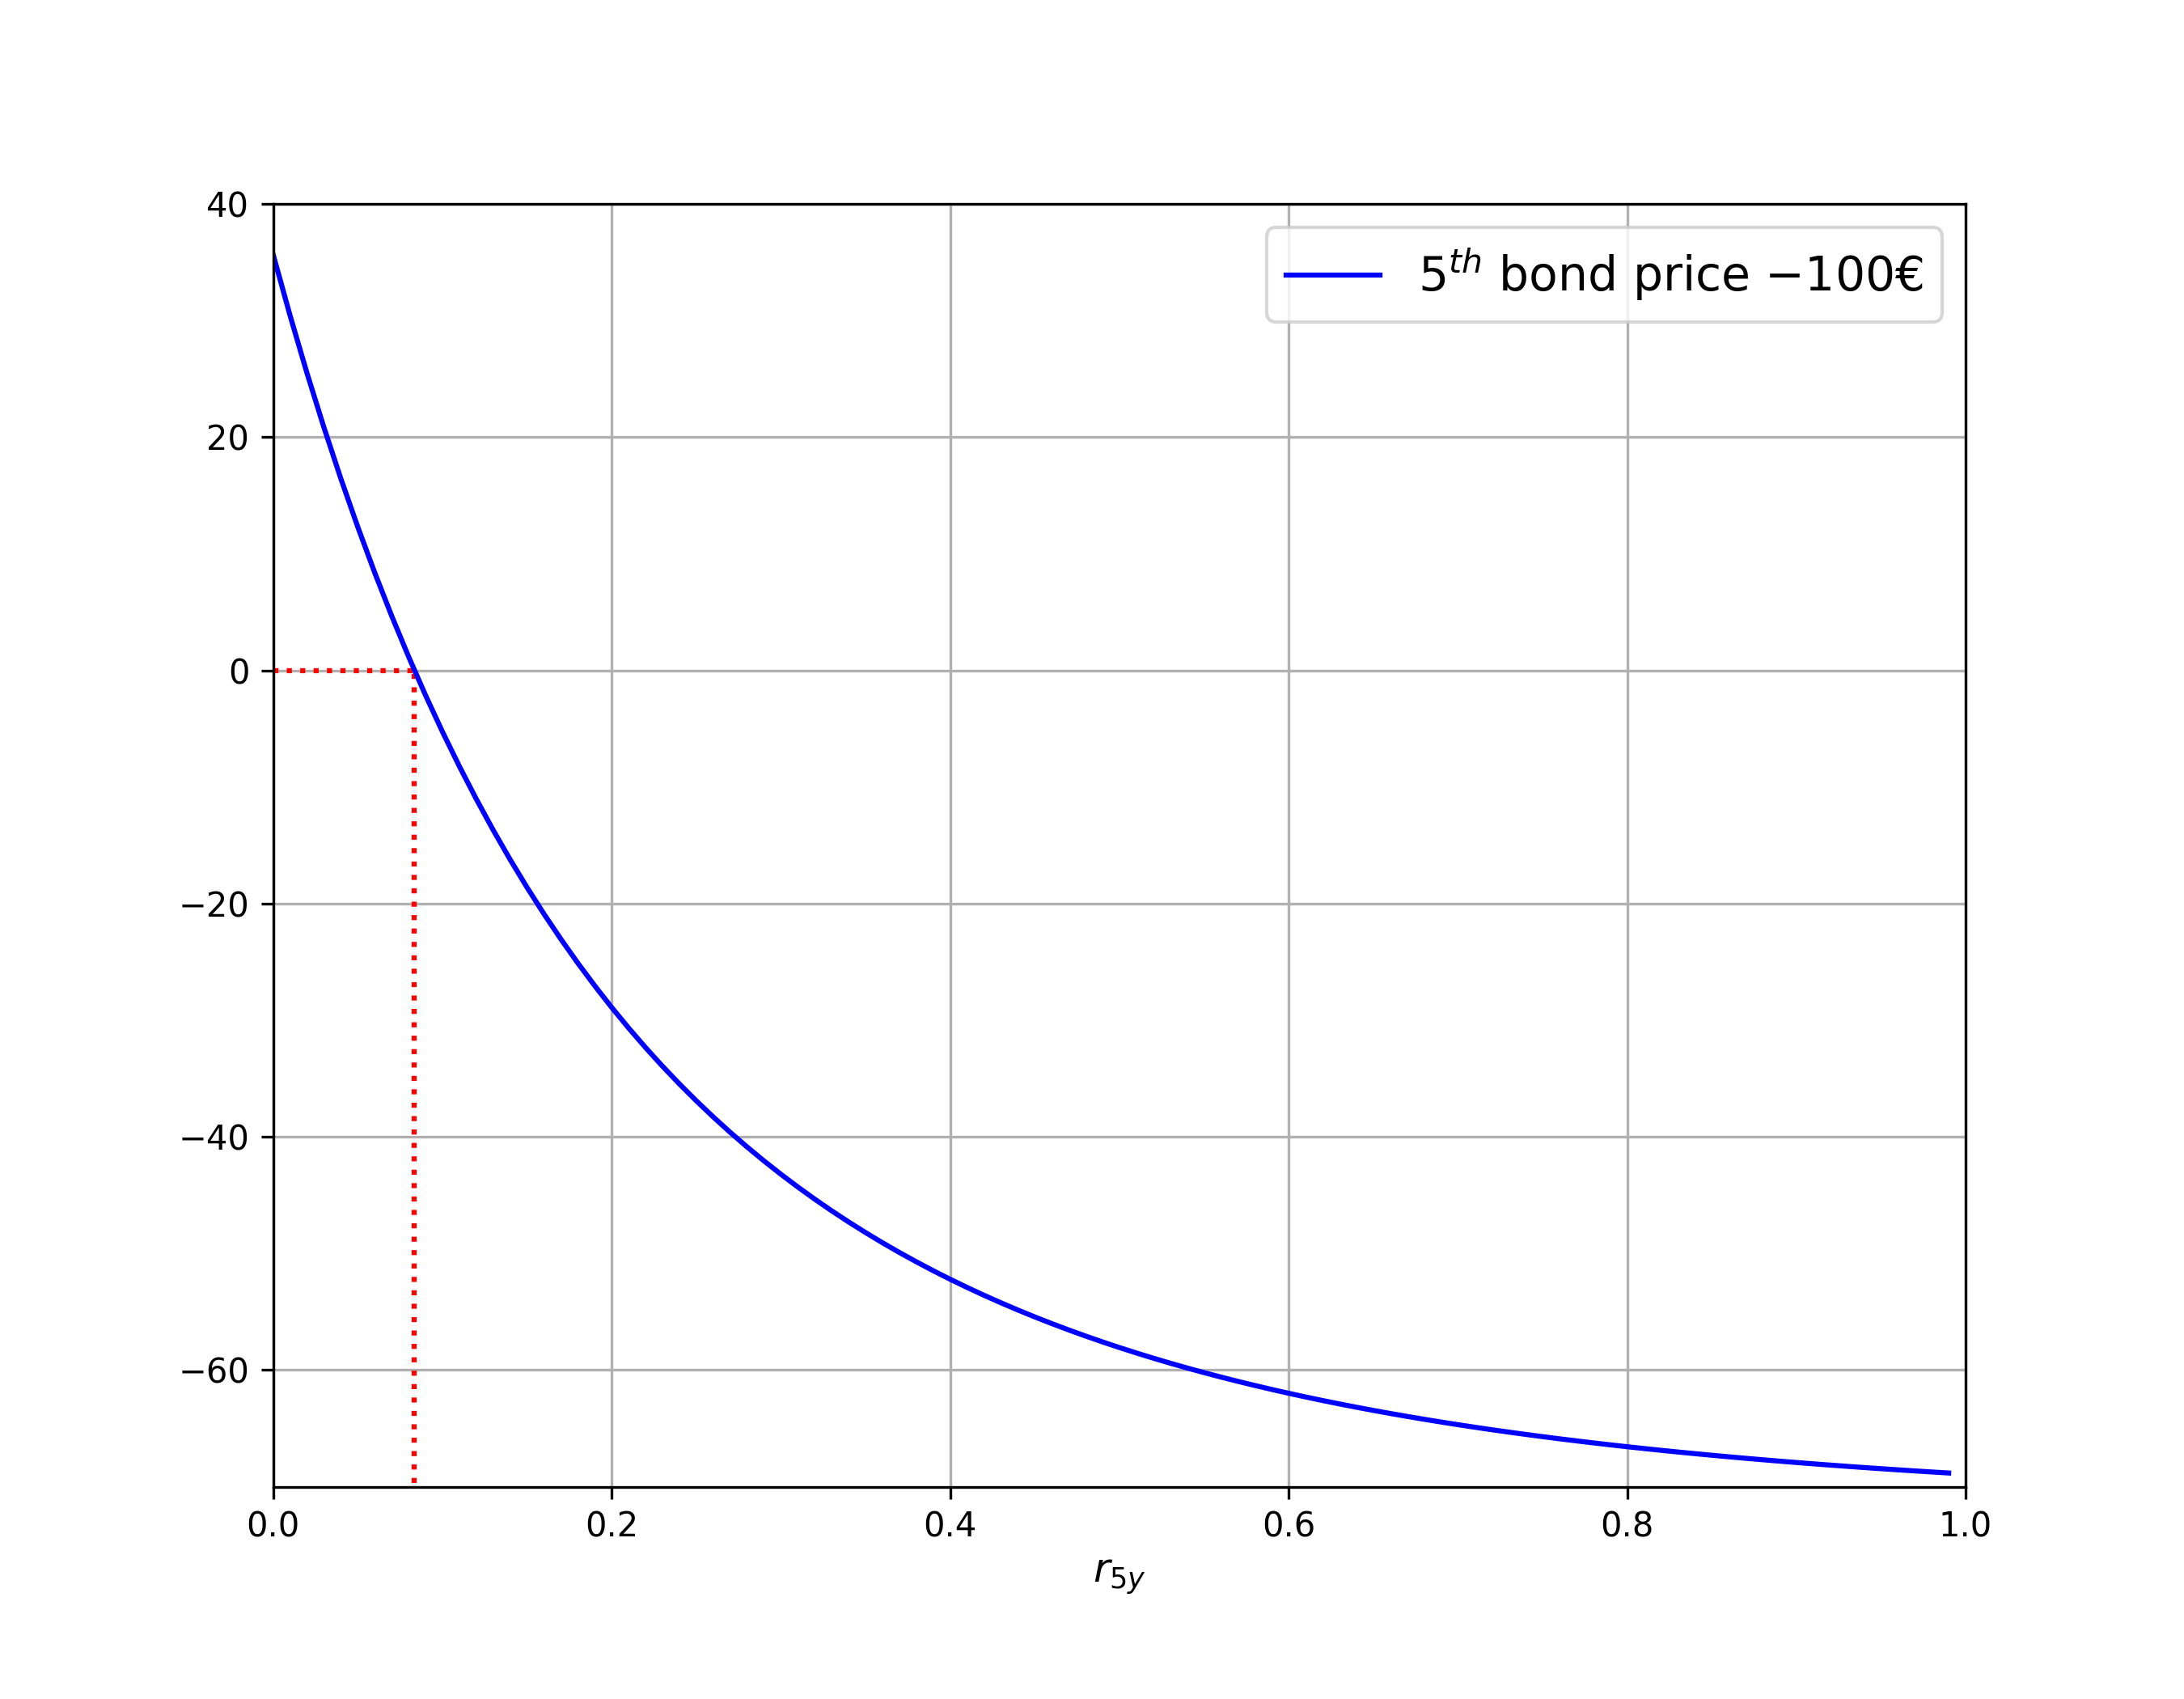
\includegraphics[width=0.7\textwidth]{figures/bond_5_plot.png}
  \caption{Plot of the discounted cash flow of bond 5 as a function of the 5 year spot rate.}
  \label{fig:fifth_year_rate}
\end{figure}

\pythoncodenon{code/bootstrap_2.py}

\begin{ioutput}
5y rate: 0.0836
\end{ioutput}

The very same mechanism can be generalized and extended to other maturities to get a more detailed yield curve. In general terms the previous system becomes

\begin{equation}
\begin{cases}
f_1(r_1, P_1) = 0 \\
f_2(r_1, r_2, P_2) = 0 \\
f_3(r_1, r_2, r_3, P_3) = 0 \\
f_4(r_1, r_2, r_3, r_4, P_4) = 0 \\
\cdots
\end{cases}
\end{equation}
where $r_i$ are the unknown spot rates and $P_i$ the market quotes of the considered products. The iterative procedure we have applied before exploits the first equation to find $r_1 = f_1^{-1}(P_1)$, the second to find $r_2 = f_2^{-1}(r_1, P_2)$ and so on. Each equation determines exactly one spot rate which is not already determined by the others.

\subsection{Bootstrapping the Discount Curve}

From what we have seen the discount curve can be \emph{bootstrapped} by successively calibrating it to return the input product market quotes.
Let's implement the outlined procedure in \texttt{python}, the first step is to choose the set of contracts to use in the minimization.

Our choice concerns a set of Overnight Index Swaps indexed on \euro STR, in Fig.~\ref{fig:icap} the used quotes.

\begin{figure}[bth]
	\centering
	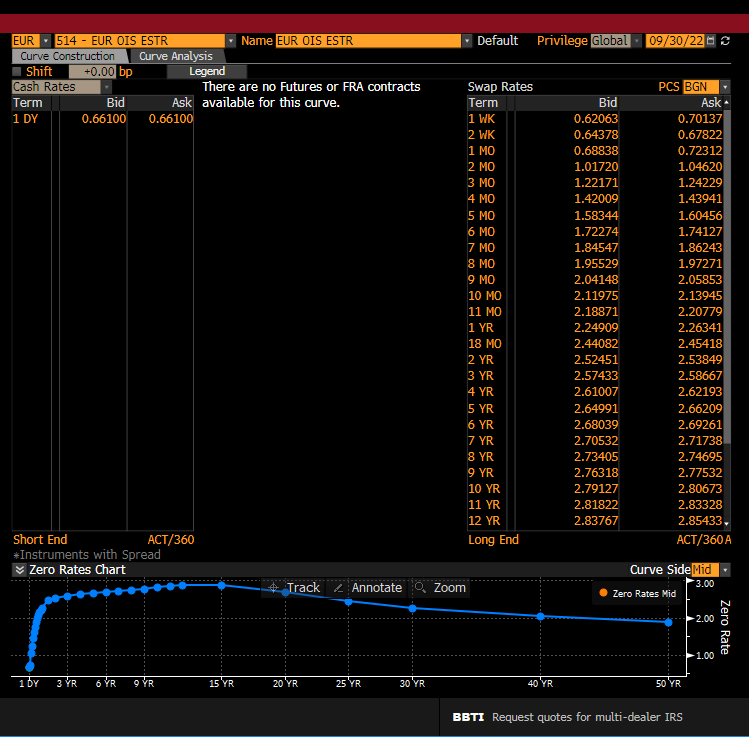
\includegraphics[width=1.\linewidth]{figures/bbg_ois}
	\caption{Screenshot of OIS market quotes from Bloomberg as of 2022-09-30.}
	\label{fig:icap}
\end{figure}

Note that interest rate swap quotes vary from standard prices of commonly traded instruments, they can be puzzling but are effectively interest rates (i.e. the rate of the fixed leg).

OIS became the standard following the 2008 financial crisis; previously, the LIBOR curve was used, but its stability was called into question when the spread between LIBOR and other "risk-free" rates, like U.S. Treasury bills, widened dramatically. The floating leg of those instruments is based on a daily compounded overnight rate and this is generally considered the best proxy for a risk-free rate because the time horizon is so short (i.e. the risk of a bank defaulting on an overnight loan is significantly lower than on a longer-term loan, like those captured by LIBOR).

In the post-crisis world, a dual-curve bootstrapping methodology is used to price derivatives. One curve, the OIS curve, is used exclusively for discounting cash flows because it represents the risk-free rate. A separate curve, often a LIBOR or SOFR curve, is used to project future cash flows of the floating-rate leg of the swap. This separation is crucial for accurately reflecting the market's funding dynamics and credit risk.

The resulting dateset is stored in (\href{https://github.com/matteosan1/finance_course/raw/master/input_files/ois_2024_10_14.xlsx}{\texttt{ois\_2024\_10\_14.xlsx}}).

\pythoncodenon{code/bootstrap_3.py}

\begin{ioutput}
  maturities    quotes
  7D          3.414000
  14D         3.295500
  1M          3.229000
  2M          3.209205
  3M          3.127103
\end{ioutput}

Now using a very simple \texttt{Bootstrap} class we are going to construct the discount curve by adding at each iteration a new pillar given by the
maturity of the corresponding OIS.

So the 7D swap depends on the discount factor seven days in advance from today.
At the beginning of the Chapter we said that the OIS market quotes represent their \emph{fair} prices (i.e. the price which buyer and seller happily agree for
the contract). The bootstrap will set it by requiring the OIS net present value to be zero (this is the objective function), task that can be easily performed
using one the root finding algorithms outlined in~\ref{sec:root_finding}.

Moving to the 14D OIS, its NPV depends on the 7D (already found) and 14D discount factors, so the second parameter will be
determined by again requiring the net present value to be 0. The process iteratively will find a new discount factor for each OIS in the list defining the entire
discount curve.

\pythoncodenon{code/bootstrap_bootstrapper.py}
\begin{ipythonnon}
from bootstrap import Bootstrapper

bootstrap = Bootstrapper(oiss)
discount_curve = bootstrap.run(DiscountCurve)
\end{ipythonnon}
\noindent
Finally we have created the discount curve implied by the market quotes of our swaps (see Fig.~\ref{fig:discount_curve}), so we can compute some implied
rates.

\pythoncodenon{code/bootstrap_4.py}

\begin{ioutput}
40y df: 0.622
\end{ioutput}

\begin{figure}[htb]
	\centering
	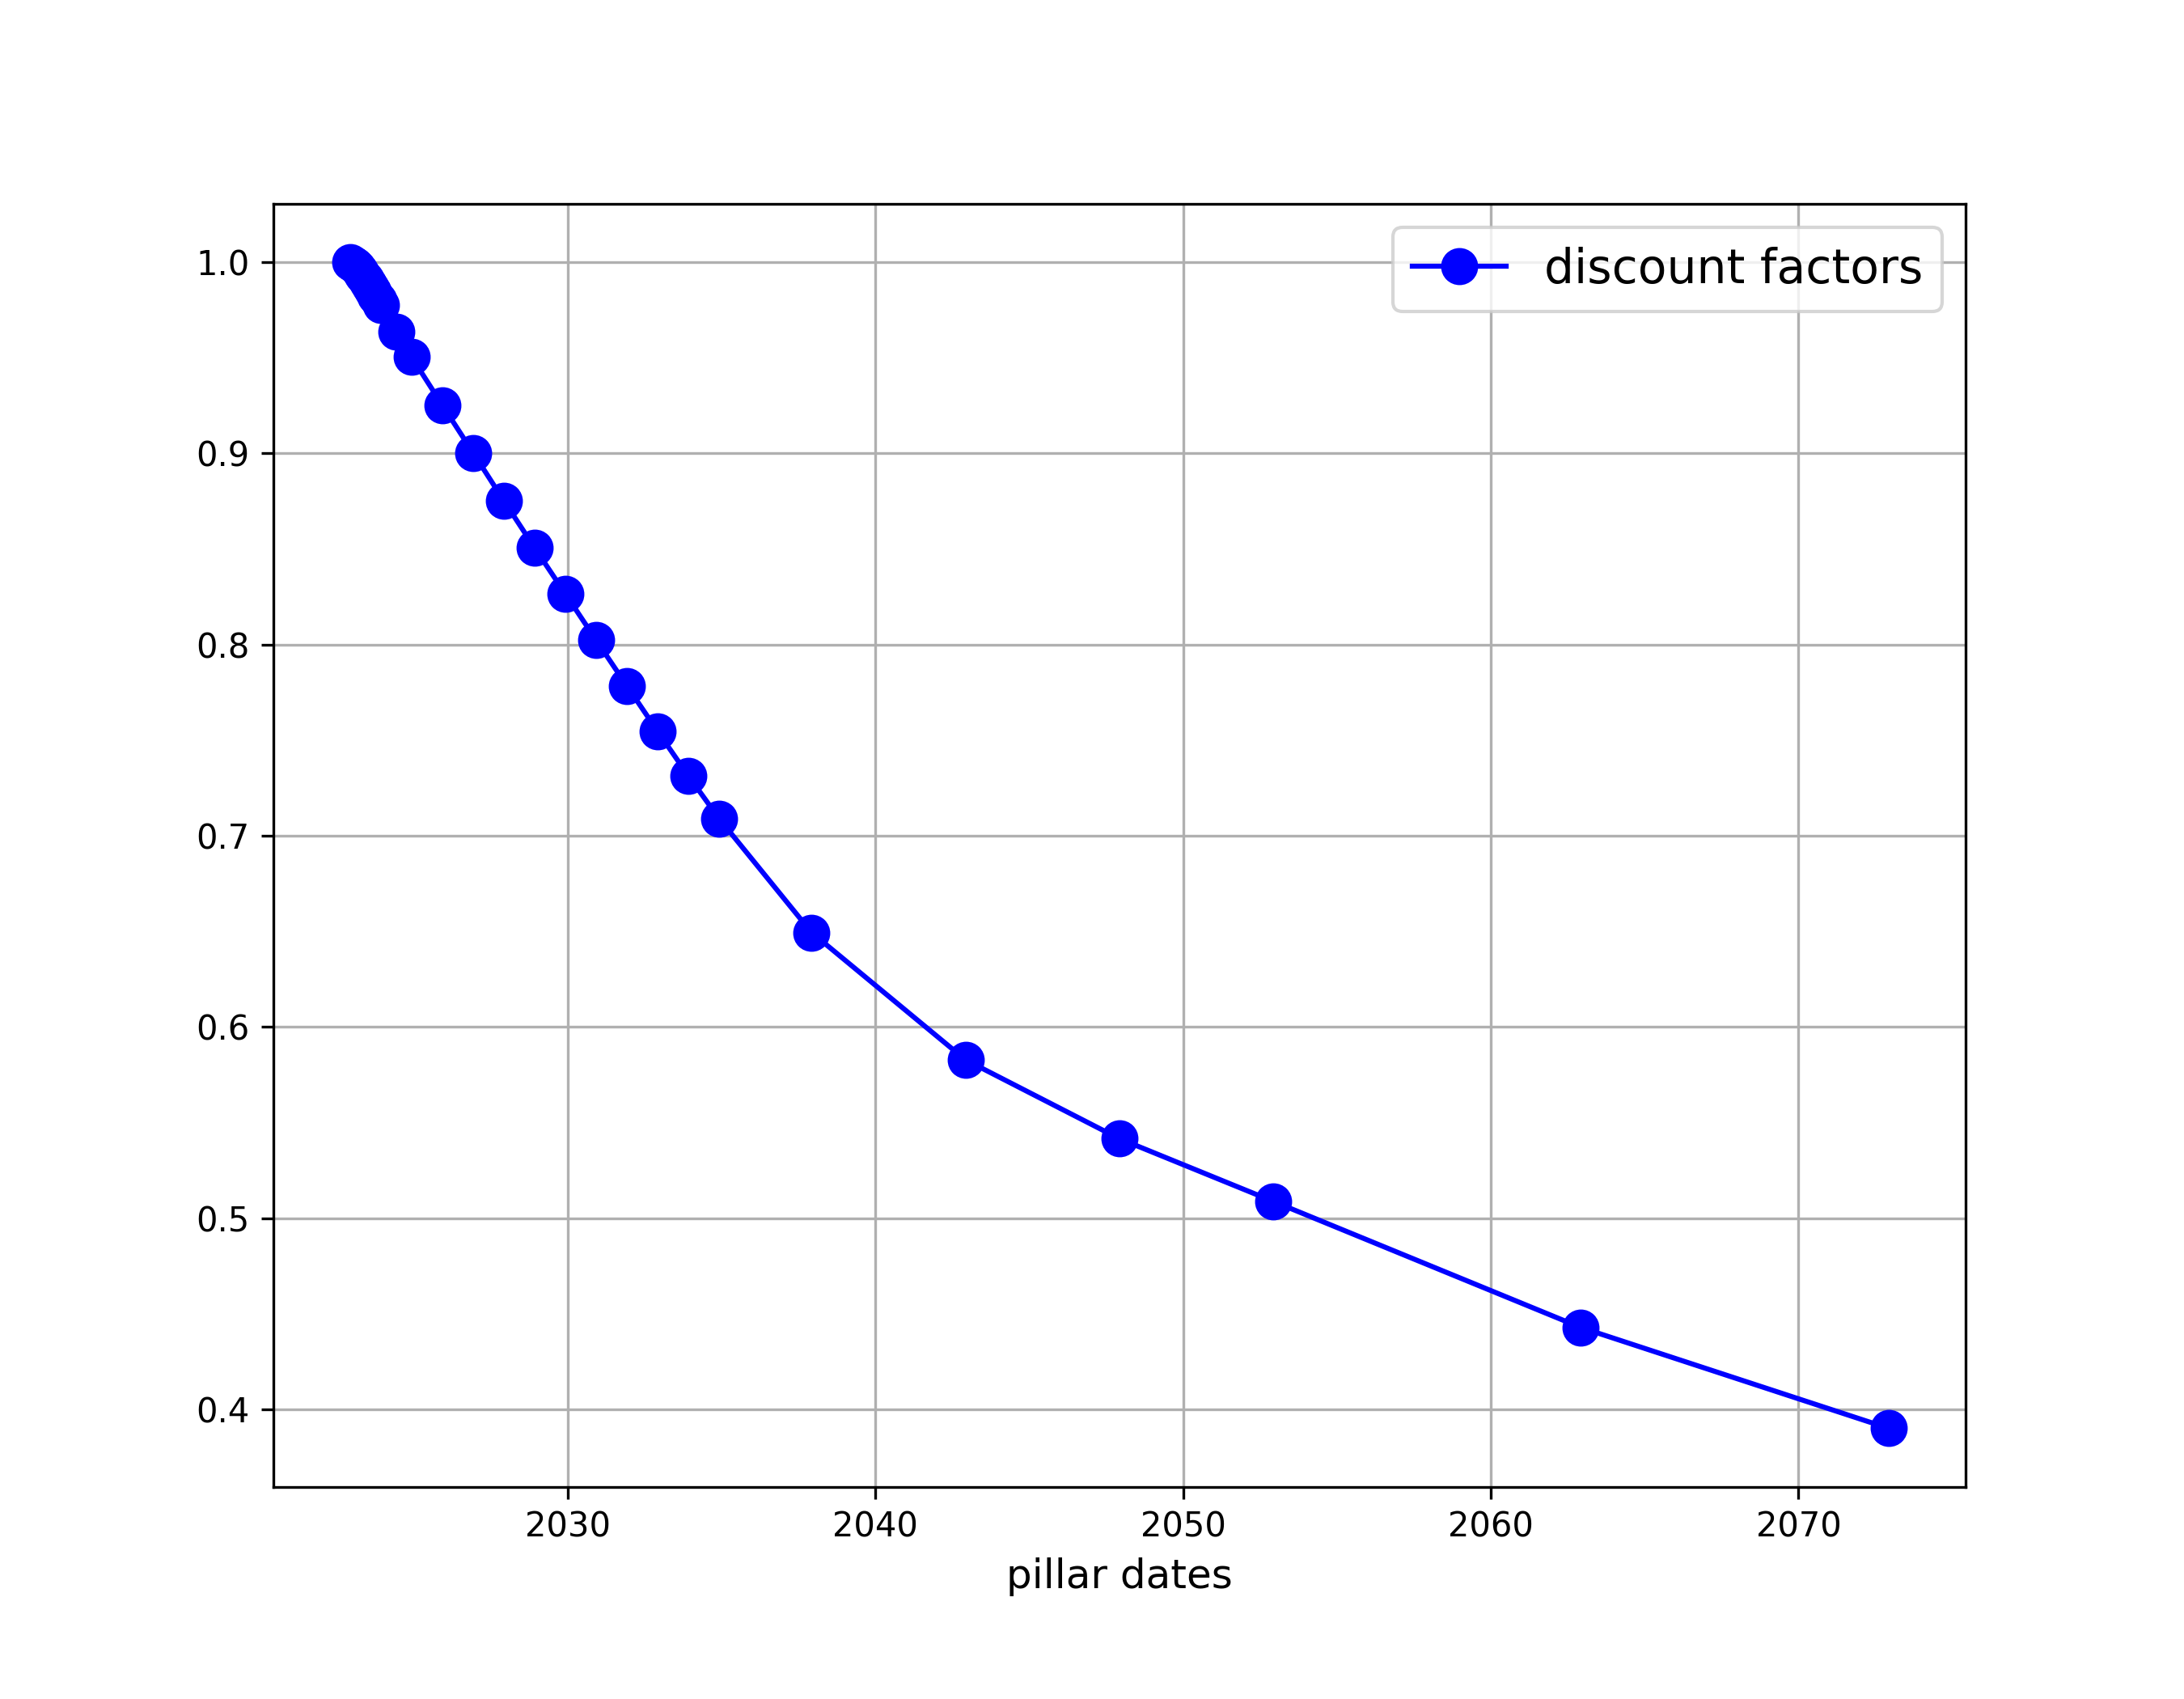
\includegraphics[width=0.7\textwidth]{figures/example_discount_curve}
	\caption{Plot of the discount curve implied by Overnight Index Swap market quotes.}
	\label{fig:discount_curve}
\end{figure}

\subsection{Bootstrap as Minimization Problem}
\label{sec:bootstrap_as_minimization}

The bootstrap algorithm can alternatively be seen under another point of view. Define a vector of spot rates $\mathbf{r} = (r_1, r_2, r_3, \ldots)$ and 
seek for a particular set $\mathbf{\hat{r}}$ which solves the following equation:

\begin{equation}
F = f_1^2(\hat{r}_1,P_1) + f_2^2(\hat{r}_1, \hat{r}_2,P_2) + f_3^2(\hat{r}_1, \hat{r}_2, \hat{r}_3,P_3) + f_4^2(\hat{r}_1, \hat{r}_2, \hat{r}_3, \hat{r}_4,P_4) + \ldots = 0
\label{eq:bootstrap_as_minimization}
\end{equation}

Solving Eq.~\ref{eq:bootstrap_as_minimization} is equivalent to find the solution of the system~\ref{eq:fifth_year_rate}.
Under this terms the bootstrap method becomes a \emph{minimization problem}. In fact we need to find $\mathbf{\hat{S}}$ which \emph{minimize} $F$,
(i.e. makes it as close as possible to 0).

This means that the OIS NPV's should be close to 0 hence the objective function~\ref{eq:bootstrap_as_minimization} becomes

\begin{equation}
\mathrm{Objective Function} = \sum_{i=1}^{n}\mathrm{NPV}^\mathrm{OIS}_i(\mathcal{C})^2
\end{equation}.

Once the OIS characteristics (e.g. nominal, maturity\ldots) have been specified the only unknown parameter in the NPV calculation is the discount
curve $\mathcal{C}$ (i.e. the minimization algorithm will adjust $\mathcal{C}$ to reach the minimum).

In previous examples the number of minimization parameters, \emph{the degrees of freedom} of the problem, were clear:
\begin{itemize}
\item 1 for the can example, the can radius;
\item 2 for the fence problem, width and height of the field.
\end{itemize}

A discount curve is characterized by a set of pillar dates ($\mathbf{d}$) and a set of discount factors ($\mathbf{x}$), but it hasn't yet been
identified any constraint on how many points the curve has to be made of (too many or too few points may prevent us from finding the solution).

In practice \textbf{it makes sense to choose the degrees of freedom to match the number of market quotes}. In particular it is wise to choose the pillar
dates of the discount curve equal to the swap expiry dates, leaving as unknown parameters just the discount factors.

The final version of the optimization problem becomes

\begin{equation}
 \mathrm{min}_{\mathbf{x}} \left\{\sum_{i=1}^{N}\mathrm{NPV}^\mathrm{OIS}_i( \mathcal{C}(\mathbf{x}))^2\right\}
\end{equation}
i.e. finding the minimum of the above expression as a function of the discount factors $\mathbf{x}$.

Notice how each $f_i$ is squared since we want all of them to be minimized at the same time and not only $F$ globally
(i.e. without the square there may be cancellation effects between the terms of the sum, which makes $F$ zero but not all $f_i$ individually).

Let's repeat the bootstrapping with the swaps defined above.
%(today's discount factor is fixed to 1 so it is not included among the minimization parameters).
Note that the objective function has constant additional parameters so they will be passed using \texttt{args} (see Section~\ref{sec:kwargs_args}).

Set the initial value of the discount factors $x_i^0$ to 1 with a range of variability $[0.01, 10]$. Discount factor 0 will be set fixed to 1.
Finally launch the minimizer to find the discount factors

\pythoncodenon{code/bootstrap_5.py}

\begin{ioutput}
  message: CONVERGENCE: NORM_OF_PROJECTED_GRADIENT_<=_PGTOL
  success: True
   status: 0
      fun: 1.547769660487322e-12
        x: [ 9.994e-01  9.983e-01 ...  4.428e-01  3.901e-01]
      nit: 7
      jac: [ 2.598e-07  4.056e-07 ...  1.766e-07  4.188e-07]
     nfev: 279
     njev: 9
 hess_inv: <30x30 LbfgsInvHessProduct with dtype=float64>
 \end{ioutput}

\subsection{Discount Factors with Pseudo-inverse}
An alternative procedure to derive discount factors involves matrix inversion and in some special cases the usage of the \emph{pseudoinverse} described in Section~\ref{sec:the-moore-penrose-pseudoinverse}. Details on this algorithm can be found in~\cite{bib:boostrap_pseudoinv}.

Consider a set of $n$ financial instruments (e.g. bonds, futures, swaps, \ldots). The price of such instruments is connected to the discount factors by the following relationship

\begin{equation}
P_i = \sum_{j=0}^{m} C_{i,j} d_j
\label{eq:discounted_cashflows}
\end{equation}
where $P_i$ is the market quote of the $i^{th}$ product, $C_{i,j}$ is the $j^{th}$ cash-flow of the $i^{th}$ product and $d_j$ is the discount factor relative to period $(t_0, t_j)$.
Eq.~\ref{eq:discounted_cashflows} can be written in matrix form

\begin{equation}
\boldsymbol{P} = [C]\boldsymbol{d}
\label{eq:discount_matrix}
\end{equation}
and now $P$ and $d$ are column vectors while $[C]$ is a $n \times m$ matrix where each row element is a cash-flow associated to the row product.

Recalling Section~\ref{solving-systems-of-equations-using-matrix-inverses}, Eq.~\ref{eq:discount_matrix} represents a system of equations which can be solved to determine the unknown $\boldsymbol{d}$.
The sought solution is
\begin{equation}
\boldsymbol{d} = [C^{-1}] \boldsymbol{P}
\end{equation}
If matrix $[C]$ is not invertible (i.e. the system of equations is under-determined) $[C^{-1}]$ can be replaced by the optimal approximation $[C^+]$ (i.e. the pseudo-inverse).

To illustrate the algorithm let's consider again the previous example with five coupon bearing bonds (coupon of 4\%, 5\%, 6\%, 7\% and 8\% respectively) with maturities ranging from 1 to 5 years, each having a value of \euro{100}. In this case we have
\begin{equation*}
\boldsymbol{P} =
\begin{bmatrix}
100 \\
100 \\
100 \\
100 \\
100
\end{bmatrix}; \quad
[C] =
\begin{bmatrix}
104 & 0 & 0 & 0 & 0 \\
5 & 105 & 0 & 0 & 0 \\
6 & 6 & 106 & 0 & 0 \\
7 & 7 & 7 & 107 & 0 \\
8 & 8 & 8 & 8 & 108
\end{bmatrix}; \quad \boldsymbol{d} =
\begin{bmatrix}
d_1 \\
d_2 \\
d_3 \\
d_4 \\
d_5
\end{bmatrix}
\end{equation*}
The \texttt{python} implementation to determine the solution is given in the snippet below. The code use by default the pseudo-inverse since if $[C]$ is invertible holds $[C^+] = [C^{-1}]$.

\pythoncodenon{code/bootstrap_pseudoinverse.py}

\begin{ioutput}
[0.96153846 0.90659341 0.83765291 0.75756548 0.66938146]
\end{ioutput}
To determine the corresponding yields just use \texttt{brentq} to solve $d=1/(1+y_n)^{n}$

\begin{ioutput}
yield y1: 0.0400
yield y2: 0.0503
yield y3: 0.0608
yield y4: 0.0719
yield y5: 0.0836
\end{ioutput}
which matches those in Table~\ref{tab:rates}.

In this simple example just bonds were considered but clearly the method can be extended also to other instruments when creating the cash-flow matrix $[C]$.

%\section*{Exercises}
%\begin{question}
Consider two 5\% coupon paying bonds (par value of 100 EUR) with the clean market prices of 99.50 EUR and 98.30 EUR and having maturities of 6 months and 1 year respectively.
Determine the spot rate for 6-month and 1-year.  
\end{question}

\cprotEnv\begin{solution}
At the end of 6 months the first bond will pay a coupon of 2.5 EUR (= 100 EUR * 5\%/ 2) plus the principal amount (= 100 EUR) which sums up to 102.50 EUR. To determine the 6M spot rate we can write the following equation,

\begin{ipython}
S_6m = 2*(102.5/99.5 - 1) 
print (S_6m)
\end{ipython}
\begin{ioutput}
0.06030150753768826
\end{ioutput}

\begin{equation*}
\cfrac{102.5}{(1 + S_{6M}/2)} = 99.5\qquad\Rightarrow\qquad S_{6M} = 2 \cdot \Big( \cfrac{102.5}{99.5} - 1 \Big) =  6.03 \%
\end{equation*}

At the end of another 6 months the second bond will pay a coupon of 2.5 EUR (= 100 EUR * 5\% / 2) plus the principal amount (= 100 EUR) which sums up to 102.50 EUR. The bond is traded at 98.30 EUR, therefore, the 1-year spot rate $S_{1y}$ can be calculated using $S_{6M}$ as,

\begin{equation*}
\cfrac{2.5}{(1+S_{6M}/2)} + \cfrac{102.5}{(1 + S_{1y}/2)^{2}} = 98.30
\end{equation*}

\begin{equation*}
\cfrac{102.5}{(1 + S_{1y}/2)^{2}} = 98.30 - \cfrac{2.5}{(1+0.03015)}
\end{equation*}

\begin{equation*}
(2 + S_{1y})^{2} = \cfrac{4\cdot102.5}{98.87317} = 4.276428
\end{equation*}

\begin{equation*}
S_{1y}^{2} + 4\cdot S_{1y} - 0.276428 = 0
\end{equation*}

\begin{ipython}
import numpy as np
coeff = [1, 4, -0.276428]
np.roots(coeff)
\end{ipython}
\begin{ioutput}
array([-4.06795261,  0.06795261])
\end{ioutput}

\begin{equation*}
S_{1y} = -2 \pm \sqrt{4 + 0.276428} =\begin{cases}\text{\sout{-4.06795}} \\ 6.80\%\end{cases}
\end{equation*}
\end{solution}

\begin{question}
A small petroleum company owns two refineries. Refinery 1 costs 20000 USD per day to operate, and it can produce 400 barrels of high-grade oil, 300 barrels of medium-grade oil, and 200 barrels of low-grade oil each day. Refinery 2 is newer and more modern. It costs 25000 USD per day to operate, and it can produce 300 barrels of high-grade oil, 400 barrels of medium-grade oil, and 500 barrels of low-grade oil each day.
The company has orders totaling 25000 barrels of high-grade oil, 27000 barrels of medium-grade oil, and 30000 barrels of low-grade oil. How many days should it run each refinery to minimize its costs and still refine enough oil to meet its orders?

\noindent\textbf{Hint:} you need to identify the unknown quantities (working days for each refinery) and set the constraints on the production of barrels. The objective is to minimize the costs. If you have multiple constraints you can define a list of dictionaries (one for constraint). Furthermore in this case the constraint is not \emph{equal to} but rather \emph{greater than} so you have to set \texttt{ineq} type.
\end{question}

\cprotEnv\begin{solution}
Let's implement the usual steps for a minimization. In this case our unknown are \texttt{x[0]} and \texttt{x[1]} the working days for each refinery. Then define the objective function with the production costs and three more functions, one for each oil-grade for the constraints.

\begin{ipython}
from scipy.optimize import minimize

def of(x):
    return 20000*x[0] + 25000*x[1]

def cons1(x):
    return 400*x[0] + 300*x[1] - 25000

def cons2(x):
    return 300*x[0] + 400*x[1] - 27000

def cons3(x):
    return 200*x[0] + 500*x[1] - 30000

cons = [{"type":"ineq", "fun":cons1},
        {"type":"ineq", "fun":cons2},
        {"type":"ineq", "fun":cons3}]
\end{ipython}
Set limits and initial values and run the minimizer.
\begin{ipython}
x0 = [10, 10]
bounds = [(0, 100) for _ in range(len(x0))]
r = minimize(of, x0, bounds=bounds, constraints=cons)
print (r)
\end{ipython}
\begin{ioutput}
     fun: 1750002.070622686
     jac: array([20000., 25000.])
 message: 'Optimization terminated successfully.'
    nfev: 8
     nit: 6
    njev: 2
  status: 0
 success: True
       x: array([25.00004033, 50.00005056])
\end{ioutput}    
So refinery 1 should work 25 days while refinery 2 50 days to minimize the production costs to 1.75 M USD (see objective function value in the minimization report).
\end{solution}

\begin{question}
Read the OIS market data from \href{https://raw.githubusercontent.com/matteosan1/finance_course/master/input_files/ois_quotes.csv}{\texttt{ois\_quotes.csv}} and construct the corresponding swaps.
\end{question}

\cprotEnv\begin{solution}

\begin{ipython}
obs_date = date.today()
df = pd.read_csv('ois_quotes.csv')
swaps = []

for i in range(len(df)):
    swap = OvernightIndexSwap(1e6,
                              obs_date,
                              "{:.0f}m".format(df.iloc[i]['maturity']),
                              df.iloc[i]['rate'])
    swaps.append(swap)
\end{ipython}
\end{solution}

\begin{question}
From the \texttt{OvernightIndexSwap} created in the previous example derive a discount curve using the bootstrap method.
\end{question}

\cprotEnv\begin{solution}
We have just created some swaps from the market quotes in the previous exercise, so now we can just create a list with the pillar dates.
Set the initial value of the discount factors ($x_i$) to 1 with a range of variability $[ 0.01, 10]$, in addition the first element of the list, today's discount factor, will be fixed to 1 (variability $[1, 1]$).
Finally launch the minimizer to find the discount factors ($\mathbf{x}$).


\begin{ipython}
obs_date = date.today()
pillar_dates = []
for swap in swaps:
    pillar_dates.append(swap.payment_dates[-1])
    pillar_dates = sorted(pillar_dates)

def objective_function(x, obs_date, pillar_dates):
    curve = DiscountCurve(obs_date, pillar_dates, x)
    sum_sq = 0.0
    for swap in swaps:
        sum_sq += swap.npv(curve)**2
    return sum_sq

x0 = [1.0 for i in range(len(pillar_dates))]
bounds = [(0.01, 10.0) for i in range(len(pillar_dates))]
bounds[0] = (1.0, 1.0)

result = minimize(objective_function, x0, bounds=bounds,
                  args=(obs_date, pillar_dates))
print (result)
\end{ipython}
\begin{ioutput}
      fun: 8331.633347139361
 hess_inv: None
      jac: array([        nan, -1.69020495, -1.75787135, -1.8173523 , -1.870103  ,
       -1.91303115, -1.94595485, -1.97032931, -1.98488123, -1.98579072,
       -1.9725121 , -7.53570926,  2.40634107,  2.07692209,  1.87283148,
       -2.06928234,  3.4475306 ,  7.70742186,  6.94308252,  3.00806276,
       -0.71722752, -2.09674907, -0.76743163,  2.65299603,  6.86359268,
        9.26702337, 13.24679026, -4.50745572, -4.37703418, -6.18147169])
  message: 'CONVERGENCE: REL_REDUCTION_OF_F_<=_FACTR*EPSMCH'
     nfev: 300
      nit: 8
     njev: 10
   status: 0
  success: True
        x: array([1.        , 0.9998132 , 0.99971258, 0.99961015, 0.99950111,
       0.999392  , 0.99928207, 0.99916369, 0.99903027, 0.998895  ,
       0.99874906, 0.99860278, 0.99807755, 0.99748218, 0.99674117,
       0.99582871, 0.9895829 , 0.97817149, 0.96223341, 0.94242757,
       0.9199792 , 0.89555418, 0.86968308, 0.84279963, 0.81599921,
       0.78928685, 0.71347125, 0.61195638, 0.53249028, 0.46683191])
\end{ioutput}

\end{solution}

\begin{question}
Consider the bearing coupon bonds listed in the next Table. Using the pseudo-inverse method determine discount factors and yields (assume continuous compounding).

\begin{table}[htb]
	\begin{center}
		\begin{tabular}{|c|c|c|}
			\hline
			\textbf{price} & \textbf{maturity} & \textbf{coupon} \\
			\hline
			96.60 EUR & 1 & 2.0\% \\
			\hline
			93.71 EUR & 2 & 2.5\% \\
			\hline
			91.56 EUR & 3 & 3.0\% \\
			\hline
			90.24 EUR & 4 & 3.5\% \\
			\hline
			89.74 EUR & 5 & 4.0\% \\
			\hline
			90.04 EUR & 6 & 4.5\% \\
			\hline
			91.09 EUR & 7 & 5.0\% \\
			\hline
 			92.82 EUR & 8 & 5.5\% \\
			\hline
			95.19 EUR & 9 & 6.0\% \\
			\hline
			98.14 EUR & 10 & 6.5\% \\
			\hline
		\end{tabular}
	\end{center}
\end{table}
	
\end{question}

\cprotEnv\begin{solution}
\begin{ipython}
import numpy as np

C = np.array([[102, 0, 0, 0, 0, 0, 0, 0, 0, 0],
              [2.5, 102.5, 0, 0, 0, 0, 0, 0, 0, 0],
              [3, 3, 103, 0, 0, 0, 0, 0, 0, 0],
              [3.5, 3.5, 3.5, 103.5, 0, 0, 0, 0, 0, 0],
              [4, 4, 4, 4, 104, 0, 0, 0, 0, 0],
              [4.5, 4.5, 4.5, 4.5, 4.5, 104.5, 0, 0, 0, 0],
              [5, 5, 5, 5, 5, 5, 105, 0, 0, 0],
              [5.5, 5.5, 5.5, 5.5, 5.5, 5.5, 5.5, 105.5, 0, 0],
              [6, 6, 6, 6, 6, 6, 6, 6, 106, 0],
              [6.5, 6.5, 6.5, 6.5, 6.5, 6.5, 6.5, 6.5, 6.5, 106.5]])

P = np.array([96.60, 93.71, 91.56, 90.24, 89.74, 
              90.04, 91.09, 92.82, 95.19, 98.14])

Cinv = np.linalg.pinv(C)
d = Cinv.dot(P.T)
print (d)
\end{ipython}
\begin{ioutput}
[0.94705882 0.89114491 0.83539212 0.7814726  0.72999737 0.68140865
 0.63578693 0.59296268 0.55300618 0.51574181]
\end{ioutput}

\begin{ipython}
import numpy as np

for i in range(10):
    print ("y{}: {:.3f}%".format(i+1, -np.log(d[i])/(i+1)*100))
\end{ipython}
\begin{ioutput}
y1: 5.439%
y2: 5.762%
y3: 5.995%
y4: 6.164%
y5: 6.294%
y6: 6.393%
y7: 6.470%
y8: 6.533%
y9: 6.582%
y10: 6.621%
\end{ioutput}
\end{solution}


\chapter{Bayesian Statistics}
\label{cap:bayes}

\emph{Bayesian statistics} is a particular approach to applying probability to statistical problems. It provides us with mathematical tools to update our beliefs about random events in light of seeing new data or evidence about those events.

In particular Bayesian inference interprets probability as a measure of confidence that an individual may possess about the occurrence of a particular event.

We may have a \emph{prior belief} about an event, but our beliefs are likely to change when \emph{new evidence} is brought to light. Bayesian statistics gives a solid mathematical means of incorporating our prior beliefs, and evidence, to produce \emph{new posterior beliefs}.

This is in contrast to another form of statistical inference, known as \emph{frequentist statistics}, which assumes that probabilities are the frequency of particular random events occurring in a long run of repeated trials.

For example, as we roll a fair six-sided die repeatedly, we would see that each number on the die tends to come up 1/6 of the time.

\section{Frequentist vs Bayesian}
When carrying out statistical inference, that is, inferring statistical information from probabilistic systems, the two approaches, frequentist and Bayesian, have very different philosophies.

Frequentist statistics tries to eliminate uncertainty by providing estimates. Bayesian statistics tries to preserve and refine uncertainty by adjusting individual beliefs in light of new evidence.

In order to make clear the distinction between the two differing statistical philosophies, we will consider two examples of probabilistic systems:
\begin{itemize}
\item Coin flips, what is the probability of an unfair coin coming up head ?
\begin{itemize}
	\item \textbf{frequentist}: the probability of seeing a head when the unfair coin is flipped is the long-run relative frequency of seeing a head when repeated flips of the coin are carried out. That is, as we carry out more coin flips the number of heads obtained as a proportion of the total flips tends to the "true" probability of the coin coming up as head. In particular the individual running the experiment does not incorporate her own beliefs about the fairness of the coin.
	\item \textbf{Bayesian}: prior to any flip of the coin an individual may believe that the coin is fair. After a few flips the coin continually comes up head. Thus the prior belief about fairness of the coin is modified to account for the fact that three heads have come up in a row and thus the coin might not be fair. After 500 flips, with 400 heads, the individual believes that the coin is very unlikely to be fair. The posterior belief is heavily modified from the prior belief of a fair coin.
\end{itemize}
\item Election of a particular candidate for UK Prime Minister, what is the probability of seeing an individual candidate winning, who has not stood before ? (i.e. the candidate only ever stands once for this particular election and so we cannot perform "repeated trials") 
\begin{itemize}
	\item \textbf{frequentist}: here we construct "virtual" trials of the election process. The probability of the candidate winning is defined as the relative frequency of the candidate winning in the "virtual" trials as a fraction of all trials.	
	\item \textbf{Bayesian}: an individual has a prior belief of a candidate's chances of winning an election and their confidence can be quantified as a probability. However another individual could also have a separate differing prior belief about the same candidate's chances. As new data arrives, both beliefs are (rationally) updated by the Bayesian procedure.
\end{itemize}
\end{itemize}

Thus in the Bayesian interpretation a probability is a summary of an individual's opinion. A key point is that different (intelligent) individuals can have different opinions (and thus different prior beliefs), since they have differing access to data and ways of interpreting it. However, as both of these individuals come across new data that they both have access to their (potentially differing) prior beliefs will lead to posterior beliefs that will begin converging towards each other under the rational updating procedure of Bayesian inference.

In the Bayesian framework an individual would apply a probability of 0 when there is no confidence in an event occurring, while she would apply a probability of 1 when she is absolutely certain of an event occurring. A probability assigned between 0 and 1 allows weighted confidence in other potential outcomes.

In order to carry out Bayesian inference, we need to utilize a famous theorem in probability known as \emph{Bayes' rule} and interpret it in the correct fashion.

\section{Conditional Probability}
\label{sec:conditional_prob}
We begin by considering the definition of \emph{conditional probability}, which gives us a rule for determining the probability of an event $A$, given the occurrence of another event $B$. For example "what is the probability of rain occurring given that there are clouds in the sky ?"
To derive the general formula let's start with an example.

A fair die is rolled. Let $A$ be the event set that the outcome is an odd number ($A={1,3,5}$). Also let $B$ be the event set that the outcome is less than or equal to $3$ ($B={1,2,3}$). What is the probability of $A$ ($P(A)$) ? And what is the probability of $A$ given $B$, the probability we get $A$ conditioned to having also $B$ and denoted with $P(A|B)$ ?

Being a simple example we can compute the result by hand:

\begin{equation}
P(A) = \cfrac{|A|}{|S|} = \cfrac{|\{1,3,5\}|}{6} = \cfrac{1}{2}\qquad\textrm{(where S is the entire sample space)}
\end{equation}

Now let's find the conditional probability of $A$ given that $B$ occurred. If we know $B$ has occurred, the outcome must be among $\{1,2,3\}$. For $A$ to also happen the outcome must be in $A\cap B = \{1,3\}$. Since all die rolls are equally likely, we argue that $P(A|B)$ must be equal to

\begin{equation}
P(A|B) = \cfrac{|A\cap B|}{|B|} = \cfrac{2}{3}
\end{equation}

To find the mathematical definition we can rewrite the calculation by dividing the numerator and denominator by the entire space of the events $|S|$ hence:

\begin{equation}
  P(A|B) = \cfrac{|A\cap B|}{|B|} = \cfrac{\cfrac{|A\cap B|}{|S|}}{\cfrac{|B|}{|S|}} = \cfrac{P(A\cap B)}{P(B)}
  \label{eq:conditional_prob}
\end{equation}

This simply states that the probability of $A$ occurring given that $B$ has occurred is equal to the probability that they have both occurred, relative to the probability that $B$ has occurred.
Or in the language of the example above: the probability of rain given that we have seen clouds is equal to the probability of rain and clouds occurring together, relative to the probability of seeing clouds at all.
See Figure~\ref{fig:conditional_prob} for a graphical interpretation of conditional probability.

\begin{figure}[tb]
  \centering
  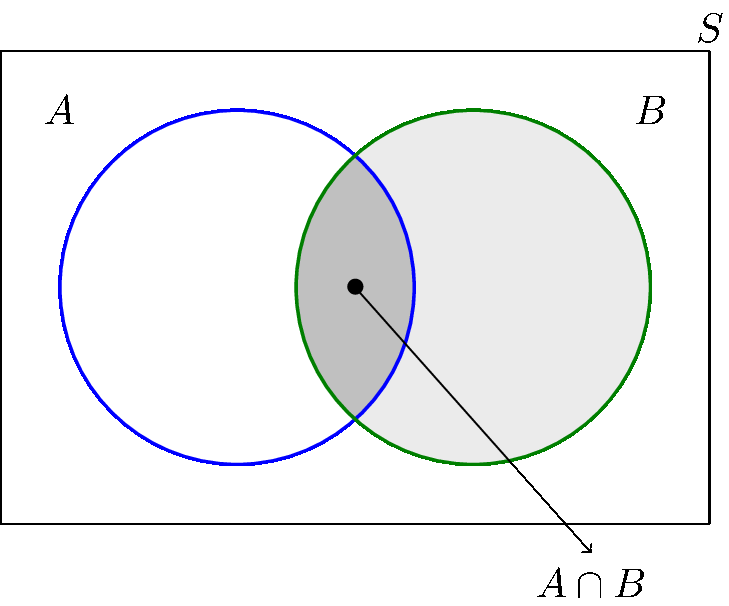
\includegraphics[width=0.5\linewidth]{figures/conditional_b}
  \caption{Graphical representation of conditional probability (the grey shaded area).}
  \label{fig:conditional_prob}
\end{figure}

\section{Bayes' Rule}

If we multiply both sides of Eq.~\ref{eq:conditional_prob} by $P(B)$ we get:
\begin{equation}
P(B)P(A|B)=P(A\cap B)
\end{equation}

What if we repeat the same reasoning applied to $P(B|A)$ instead, which is akin to asking "what is the probability of seeing clouds, given that it is raining ?"

\begin{equation}
  P(B|A)=\frac{P(B\cap A)}{P(A)}
\end{equation}
Note that $P(A\cap B) = P(B\cap A)$ (i.e. having together events $A$ and $B$ is the same as having together events $B$ and $A$) and so by substituting the above and multiplying by $P(A)$, we get:
\begin{equation}
  P(A)P(B|A)=P(A\cap B)
\end{equation}
We are now able to set the two expressions for $P(A\cap B)$ equal to each other:
\begin{equation}
  P(A)P(B|A)=P(B)P(A|B)
\end{equation}
If we now divide both sides by $P(B)$ we arrive at the celebrated Bayes' rule:
\begin{equation}
  P(A|B)=\frac{P(B|A)P(A)}{P(B)}
\end{equation}

However, it will be helpful for later usage to modify the denominator, $P(B)$ on the right hand side to be written in terms of $P(B|A)$. From the \emph{law of total probability} we can actually write:
\begin{equation}
P(B)=\sum_{a\in A}P(B\cap a)
\end{equation}
this is possible if the events $A$ are an exhaustive partition of the sample space. So that by substituting the definition of conditional probability we get:
\begin{equation}
P(B)=\sum_{a\in A}P(B\cap a) = \sum_{a\in A}P(B|a)P(a)  
\end{equation}

Finally, we can substitute this into Bayes' rule from above to obtain an alternative version, which is used heavily in Bayesian inference:
\begin{equation}
P(A|B)=\frac{P(B|A)P(A)}{\sum_{a\in A}P(B|A)P(A)}
\end{equation}

\section{Applying Bayes' Rule for Bayesian Inference}
The basic idea of Bayesian inference is to continually update our prior beliefs about events as new evidence is presented. This is a very natural way to think about probabilistic events. As more and more evidence is accumulated our prior beliefs are steadily "washed out" by any new data.

Consider a (rather nonsensical) prior belief that the Moon is going to collide with the Earth. For every night that passes, the application of Bayesian inference will tend to correct our prior belief to a posterior belief that the Moon is less and less likely to collide with the Earth, since it remains in orbit.

In order to demonstrate a concrete numerical example of Bayesian inference it is necessary to introduce some new notation.

Firstly, we need to consider the concept of \emph{parameters} and \emph{models}. A \emph{parameter} could be the weighting of an unfair coin, which we could label as $\theta$. Thus $\theta = P(H)$ would describe the probability distribution of our beliefs that the coin will come up as head ($H$) when flipped. The \emph{model} is the actual means of encoding this flip mathematically. In this instance, the coin flip can be modelled as a \emph{Bernoulli trial}. A Bernoulli trial is a random variable with only two outcomes, usually labelled as "success" or "failure", in which the probability of success is exactly the same every time the trial is carried out. This probability is given by $\theta$, and is a number between 0 and 1 $\theta\in[0,1]$.

Over the course of carrying out some coin flip experiments (repeated Bernoulli trials) we will generate some data, $D$, about heads or tails. A natural question to ask is "what is the probability of seeing 3 heads in 8 flips (8 Bernoulli trials), given a fair coin ($\theta=0.5$) ?".

%A model helps us to ascertain the probability of seeing this data, $D$, given a value of the parameter $\theta$.
The probability of seeing data $D$ under a particular value of $\theta$ is given by $P(D|\theta)$. However, if you consider it for a moment, we are actually interested in the alternative question, "what is the probability that the coin is fair (or unfair), given that I have seen a particular sequence of heads and tails ?".

Thus we are interested in the \emph{probability distribution} which reflects our belief about different possible values of $\theta$, given that we have observed some data $D$, denoted by $P(\theta|D)$. Notice that this is the converse of $P(D|\theta)$. The Bayes' rule is the link that allows to go between the two situations.
\begin{equation}
  P(\theta|D) = P(D|\theta)P(\theta)/P(D)
\end{equation}
where:
\begin{itemize}
\item $P(\theta)$ is the \emph{prior}. This is the strength in our belief of $\theta$ without considering the evidence. Our prior view on the probability of how fair the coin is.
\item $P(\theta|D)$ is the \emph{posterior}. This is the (refined) strength of our belief of $\theta$ once the evidence $D$ has been taken into account. After seeing 4 heads out of 8 flips, say, this is our updated view on the coin fairness.
\item $P(D|\theta)$ is the \emph{likelihood}. This is the probability of seeing the data $D$ as generated by a model with parameter $\theta$. If we knew the coin was fair, this tells us the probability of seeing a number of heads in a particular number of flips.
\item $P(D)$ is the \emph{evidence}. This is the probability of the data as determined by summing (or integrating) across all possible values of $\theta$, weighted by how strongly we believe in those particular values of $\theta$. If we had multiple views of what the coin fairness is (but didn't know for sure), then this tells us the probability of seeing a certain sequence of flips for all possibilities of our belief.
\end{itemize}

The entire goal of Bayesian inference is to provide us with a rational and mathematically sound procedure for incorporating our prior beliefs, with any evidence at hand, in order to produce an updated posterior belief. What makes it such a valuable technique is that posterior beliefs can themselves be used as prior beliefs under the generation of new data. Hence Bayesian inference allows us to continually adjust our beliefs under new data by repeatedly applying Bayes' rule.

Note that in the derivation of the Bayes Theorem we have used the conditional probability definition. Indeed Bayes's formula actually connects two different conditional probabilities $P(A|B)$ and $P(B|A)$, and is essentially a formula for "turning the conditioning around". The Reverend Thomas Bayes referred to this in terms of "inverse probability".

Let's see now a concrete example using the age-old tool of statisticians: the coin-flip.

\subsection{Coin-Flipping Example}
Consider multiple flips of a coin with unknown fairness. We will use Bayesian inference to update our beliefs on the fairness of the coin as more data (i.e. more coin flips) becomes available. The coin will actually be fair, but we won't learn this until the trials are carried out. At the start we have no prior belief on the fairness of the coin, that is, we can say that any level of fairness is equally likely (uniform distribution).

In statistical language we are going to perform $N$ repeated Bernoulli trials with $\theta=0.5$. %We will use a \emph{uniform distribution} as a means of characterising our prior belief that we are unsure about the fairness. This states that we consider each level of fairness (or each value of $\theta$) to be equally likely.
We are going to use a Bayesian updating procedure to go from our prior beliefs to posterior beliefs as we observe new coin flips. 
This process can be quite complicated in the general case but for this particular example the concept of \emph{conjugate priors} can be used.

\subsection{Conjugate Priors}
We have just outlined Bayes' rule and have seen that we must specify a likelihood function, a prior belief and the evidence (i.e. a normalizing constant). Let's take a closer look to the likelihood using again the coin-flips example.

We are interested in the probability of the coin coming up head as a function of the underlying fairness parameter $\theta$.
If we denote by $k$ the random variable that describes the result of the coin toss, which is drawn from the set $\{1, 0\}$, where $k=1$ represents a head and $k=0$ represents a tail, then the probability of seeing a head, with a particular fairness of the coin, is given by:
\begin{equation}
  P(k=1|\theta) = \theta 
\end{equation}
And the probability of coming up tail as:
\begin{equation}
  P(k=0|\theta) = 1-\theta 
\end{equation}
This can also be written as:
\begin{equation}
  P(k|\theta) = \theta^k(1-\theta)^{1-k} 
\end{equation}

This is known as the \emph{Bernoulli distribution}, in essence it tells us the probability of a coin coming up head or tail depending on how fair the coin is.

We can also consider another way of looking at the above function. If we consider a fixed observation, i.e. a known coin flip outcome, $k$, and the fairness parameter $\theta$ as a continuous variable then it tells us the probability of a fixed outcome $k$ given some particular value of $\theta$. As we adjust $\theta$ (e.g. change the fairness of the coin), we will start to see different probabilities for $k$.

This is known as the \emph{likelihood function} of $\theta$. Note that the likelihood function is not actually a probability distribution in the true sense since integrating it across all values of the fairness parameter $\theta$ does not actually equal 1, as is required for a probability distribution.

With the Bernoulli likelihood function we can determine the probability of seeing a particular sequence of flips, given by the set $\{k_1,\ldots,k_N\}$. Since each of these flips is independent of any other, the probability of the sequence occurring is simply the product of the probability of each flip occurring.

If we have a particular fairness parameter $\theta$, then the probability of seeing this particular stream of flips, given $\theta$, is given by:
\begin{equation}
  P(\{k\}|\theta)=\prod_{i}P(k_i|\theta)=\prod_i \theta^{k_i}(1-\theta)^{1-k_i}
\end{equation}

What about if we are interested in the number of heads, say, in $N$ flips? If we denote by $z$ the number of heads appearing, then the formula above becomes:
\begin{equation}
  P(z,N|\theta) = \binom{N}{z}\theta^z(1-\theta)^{N-z}
\end{equation}
where $\binom{N}{z}$ is the binomial coefficient. That is, the probability of seeing $z$ heads, in $N$ flips, assuming a fairness parameter $\theta$. 

\subsubsection{Quantifying our Prior Beliefs}
In the Bayesian approach we need to determine our prior beliefs on parameters and then find a probability distribution that quantifies these beliefs.
In this example we are interested in our prior beliefs on the fairness of the coin. That is, we wish to quantify our uncertainty in how biased the coin is. $\theta=0$ indicates a coin that always comes up tail, while $\theta=1$ implies a coin that always comes up head. A fair coin is denoted by $\theta=0.5$.

The question then becomes, which probability distribution do we use to quantify our beliefs about the coin ?

In this instance we are going to choose the \emph{beta distribution}. The probability density function of the beta distribution is given by:
\begin{equation}
	P(\theta|\alpha,\beta)=\theta^{\alpha -1}(1-\theta)^{\beta-1}/B(\alpha,\beta)
\end{equation}
where the term in the denominator, $B(\alpha,\beta)$ is present to act as a normalizing constant so that the area under the PDF actually sums to 1.

\begin{figure}[htb]
  \centering
  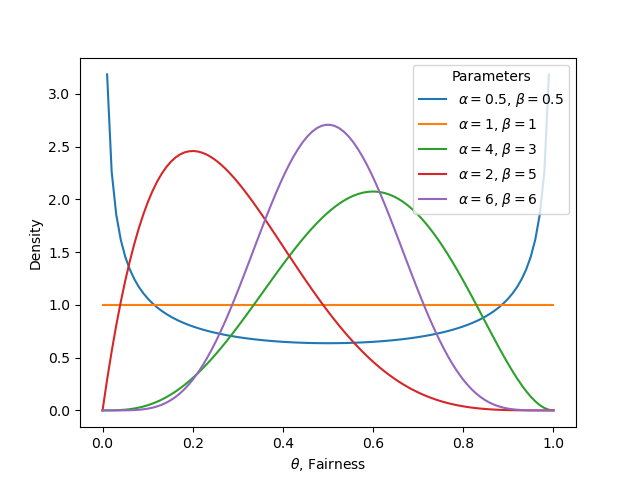
\includegraphics[width=.7\textwidth]{figures/beta_distro}
  \caption{Different realizations of the beta distribution for various parameters $\alpha$ and $\beta$.}
  \label{fig:beta_distro}
\end{figure}

Essentially, as $\alpha$ becomes larger the bulk of the probability distribution moves towards the right (a coin biased to come up heads more often), whereas an increase in $\beta$ moves the distribution towards the left (a coin biased to come up tails more often).
However, if both parameters increase then the distribution begins to narrow. If they both increase equally, then the distribution will peak over $\theta=05$, i.e. when the coin is far. Note also that the \emph{uniform distribution} is a particular case of a beta distribution (i.e. $\alpha = \beta = 1$).

Among various interesting properties we have chosen the beta function as our prior because it is a conjugate prior for the Bernoulli distribution.

\subsubsection{Conjugate Prior}
In Bayes' rule we can see that the posterior distribution is proportional to the product of the prior distribution and the likelihood function:
\begin{equation}
  P(\theta|D)\propto P(D|\theta)P(\theta)
\end{equation}

A \emph{conjugate prior} is a choice of prior distribution, that when coupled with a specific type of likelihood function, provides a posterior distribution that is of the \emph{same family} as the prior distribution, i.e. the prior and posterior both have the same probability distribution family, but with differing parameters.

Conjugate priors are extremely convenient from a calculation point of view as they provide closed-form expressions for the posterior, thus negating any complex numerical integration.

In our case, if we use a Bernoulli likelihood function AND a beta distribution as the choice of our prior, we immediately know that the posterior will also be a beta distribution.

%Using a beta distribution for the prior in this manner means that we can carry out more experimental coin flips and straightforwardly refine our beliefs. The posterior will become the new prior and we can use Bayes' rule successively as new coin flips are generated.

We can actually use a simple calculation to prove why the choice of the beta distribution for the prior, with a Bernoulli likelihood, gives a beta distribution for the posterior.

As mentioned above, the probability density function of a beta distribution, for our particular parameter $\theta$, is given by:
\begin{equation}
  P(\theta|\alpha,\beta)=\theta^{\alpha -1}(1-\theta)^{\beta-1}/B(\alpha,\beta)
\end{equation}

You can see that the form of the beta distribution is similar to the form of a Bernoulli likelihood. In fact, if we multiply the two together, we get:
\begin{equation}
  \theta^{\alpha -1}(1-\theta)^{\beta-1}/B(\alpha,\beta)\times \theta^k(1-\theta)^{1-k} \propto \theta^{\alpha+k-1}(1-\theta)^{\beta+k}
\end{equation}

Notice that the term on the right hand side of the proportionality sign has the same form as our prior (up to a normalizing constant).

The last issue we need to address is how to connect $\alpha$ and $\beta$ parameters to more intuitive parameters like mean and variance. It turns out that we can use the following relationships:
\begin{equation}
  \begin{gathered}
    \mu = \frac{\alpha}{\alpha+\beta} \\
    \sigma = \sqrt{\frac{\alpha\beta}{(\alpha + \beta)^2(\alpha + \beta + 1)}}
  \end{gathered}
\end{equation}

Re-arrange these formulae 
\begin{equation}
  \begin{gathered}
    \alpha = \left(\frac{1-\mu}{\sigma^2} - \frac{1}{\mu} \right) \mu^2\\
    \beta = \alpha\left(\frac{1}{\mu}-1 \right)
  \end{gathered}
\end{equation}

%Note that we have to be careful here, as we should not specify a , since this is the standard deviation of a uniform density (which itself implies no prior belief on any particular fairness of the coin).

So suppose I think the fairness of the coin is around 0.5, but I'm not particularly certain, I may specify a standard deviation of about 0.1. Plugging in the numbers into the above formulae gives us $\alpha = 12$ and $\beta = 12$ and the beta distribution in this instance looks like the following:
\begin{figure}[htb]
  \centering
  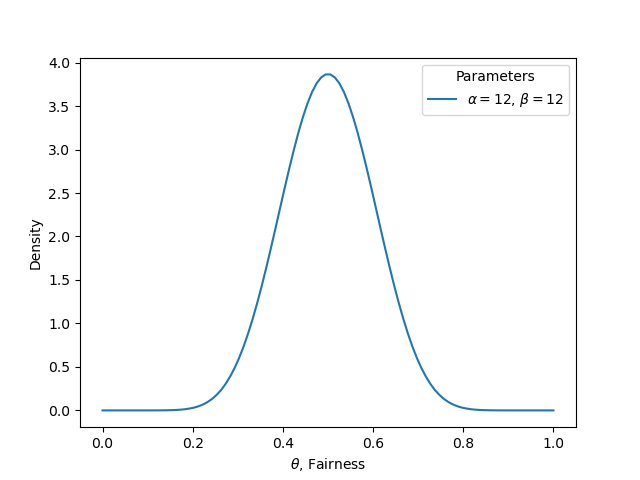
\includegraphics[width=.7\textwidth]{figures/beta_12_12}
  \caption{A beta distribution with $\alpha=12$ and $\beta=12$.}
  \label{fig:beta_12_12}
\end{figure}

Notice how the peak is centred around 0.5 but that there is significant uncertainty in this belief, represented by the curve width.

\subsection{Using Bayes' Rule to Calculate a Posterior}

We are now finally in a position to be able to calculate our posterior beliefs using Bayes' rule for repeated coin-flips
\begin{equation}
  P(\theta|z,N)=P(z,N|\theta)P(\theta)/P(z,N)
\end{equation}

If we substitute in the values for the likelihood function calculated above, as well as our prior belief beta distribution, we get:
\begin{equation}
  P(\theta|z,N)\propto P(z,N|\theta)P(\theta)\propto \theta^{z+\alpha - 1}(1-\theta)^{N-z+\beta -1} 
\end{equation}
so the posterior is given by $\textrm{beta}(\theta|z+\alpha,N-z+\beta)$ .
All we need do is specify the mean and standard deviation of our prior beliefs, carry out $N$ flips and observe the number of heads $z$ and we automatically have a rule for how our beliefs should be updated.

In Fig.~\ref{fig:bayes} we can see six particular points at which we have carried out a number of coin flips. In the top-left plot we have carried out no trials and our probability density function (in this case our original prior density) is the uniform distribution.
Originally we were not able to assume anything about the coin fairness, so the result states that we have equal belief in all values of $\theta$.

The next plot shows 2 trials carried out and they both come up heads. Our Bayesian procedure allows us to update to a posterior density. Notice how the weight of the density is now shifted to the right hand side of the chart. This indicates that our prior belief of equal likelihood of fairness of the coin, coupled with 2 new data points, leads us to believe that the coin is more likely to be unfair (biased towards heads than it is tails).

The following two plots show 10 and 20 trials respectively. Notice that since we have seen 6 tails in 10 trials we are now more convinced that the coin is likely to be unfair and biased towards tails. After 20 trials, we have seen a few more heads appear. The density of the probability has now shifted closer to $\theta = P(H) = 0.5$. Hence we are now starting to believe that the coin is possibly fair.

After 50 and 500 trials respectively, we are now beginning to believe that the coin fairness is very likely to be around $\theta=0.5$. This is indicated by the shrinking width of the probability density, which is now clustered tightly around $\theta=0.5$ in the final panel. Were we to carry out another 500 trials (since the coin is actually fair) we would see this probability density become even tighter and centred closer to $\theta=0.5$.

Thus it can be seen that Bayesian inference gives us a rational procedure to go from an uncertain situation with limited information to a more certain situation with significant amounts of data.

\begin{finmarkets}
Below code implements the coin fairness example described in the text.
\end{finmarkets}

\pythoncode{code/bayes_1.py}

\begin{figure}[htb]
  \centering
  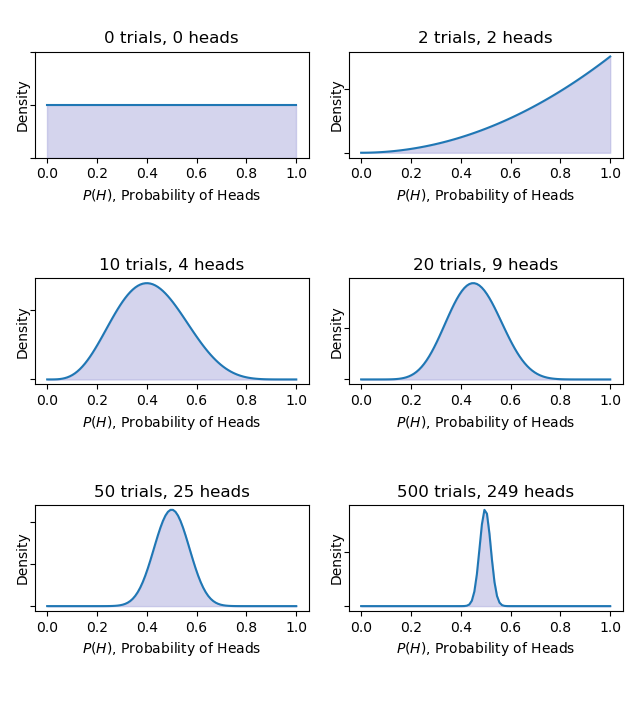
\includegraphics[width=.7\textwidth]{figures/bayes}
  \caption{Bayesian update procedure using the Beta-Binomial model.}
  \label{fig:bayes}
\end{figure}

%\section*{Exercises}
%\cprotEnv\begin{question}
Using the function \texttt{randint} of the module \texttt{random} make a Monte Carlo simulation of rolling three dice to check the probability of getting the same values on the three of them.
From probability theory you should expect:

\begin{equation*}
P_{d1=d2=d3} = \frac{1}{6}\cdot\frac{1}{6}\cdot\frac{1}{6}\cdot 6 = \frac{1}{36} = 0.0278
\end{equation*}
\end{question}

\cprotEnv\begin{solution}
\begin{ipython}
from random import seed, randint

seed(1)
trials = 10000000
success = 0

for _ in range(trials):
    d1, d2, d3 = randint(1, 6), randint(1, 6), randint(1, 6)
    if d1 == d2 and d2 == d3:
        success += 1

print ("The probability to get three equal dice is {:.4f}".format(success/trials))
\end{ipython}
\begin{ioutput}
The probability to get three equal dice is 0.0278
\end{ioutput}
\end{solution}

\begin{question}
Two fair dice are rolled, find the probability that their sum is:
\begin{enumerate}[start=1]
\item equal to 1;
\item equal to 4;
\item less than 13.
\end{enumerate}
	
\noindent\textbf{Hint:} the possible combinations of the outcomes of two dice are 36 (to realize it you can simply think that for each one of the six faces of the first die you have six possible faces of the second hence $6\cdot 6=36$). It is not possible to get 1 since the dice have no face with 0 so the first probability should come out 0. The sum of the two dice is always less than 13 (the maximum is 12\ldots) so the answer to point 3 is 1. We can get a sum of 4 in 3 cases (1-3, 3-1 or 2-2) so the expected probability is $3/36=1/12=0.0833$
\end{question}

\cprotEnv\begin{solution}
\begin{ipython}
import random

random.seed(1)
successes = {"=1":0.0, "=4":0.0, "<13":0.0}
trials = 100000

for _ in range(trials):
    d1 = random.randint(1, 6)
    d2 = random.randint(1, 6)

    if (d1 + d2) == 1:
        successes["=0"] += 1.0
    if (d1 + d2) == 4:
        successes["=4"] += 1.0
    if (d1 + d2) < 13:
        successes["<13"] += 1.0

for k,v in successes.items():
    print ("P({}): {:.3f}".format(k, v/trials))
\end{ipython}
\begin{ioutput}
P(=1): 0.000
P(=4): 0.084
P(<13): 1.000
\end{ioutput}
\end{solution}

\begin{question}
Let’s assume we have a process constructed from 3 stages $(X1, X2, X3)$. Each one has an average duration (5, 10 and 15 minutes) which vary following the normal distribution and we know their variance (all 1 minute).

We want to know what is the probability that the process will exceed 34 minutes?
\end{question}

\cprotEnv\begin{solution}
We know all the individual components so let’s define the relationship between them:

\begin{equation*}
Y = X_1 + X_2 + X_3
\end{equation*}

The single-component can be represented with a short function
\begin{ipython}
import numpy as np

def mc_normal(mean, std_dev, samples):
    results = []
    for _ in range(samples):
        results.append(np.random.normal(mean, std_dev))
    return np.array(results)
\end{ipython}

The Monte Carlo simulation code shown below uses this function as a basic block. The number of iterations for this use case is set at 10000 but you can change it. The last section of a code checks the probability of exceeding the limit of 34 minutes. Note how this can be computed when using \texttt{numpy.array}: \texttt{total > upper\_limit} returns an array with 1 or 0 depending on each element of total is greater then the limit or not; the element sum of the new array gives the number of "successes". 

\begin{ipython}
s = 100000

upper_limit = 34

component_1 = mc_normal(5,1,s)
component_2 = mc_normal(10,1,s)
component_3 = mc_normal(15,1,s)

total = component_1 + component_2 + component_3
probability = np.sum(total > upper_limit)/len(total)*100
print("Probability of exceeding the time limit: ", round(probability, 3), "%")
\end{ipython}

After running the following code we get an answer but it will vary every time you run the code:
\begin{ioutput}
Probability of exceeding the time limit:  1.016 %
\end{ioutput}

Now we can plot the histogram of the estimated parameter (time). We clearly see it follows the normal distribution.

\begin{figure}[htbp]
	\begin{center}
		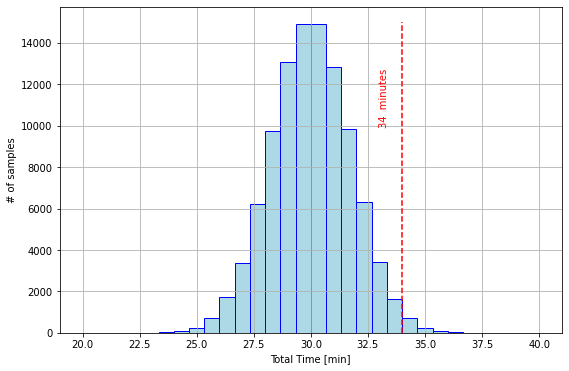
\includegraphics[width=0.7\linewidth]{figures/mc_processes}
	\end{center}
	\caption{Distribution of estimated times for the total process.}
	\label{fig:mc_processes}
\end{figure}
\end{solution}

\begin{question}
Write a Greedy Pig (see Ex.~\ref{ex:greedy_pig}) Monte Carlo simulation for a player aiming at $k$ points each turn (i.e. the turn simulation goes on until a 1 is rolled or $k$ points are reached).
Plot the distribution of the average number of points as a function of $k$.
\end{question}
\cprotEnv\begin{solution}
\begin{ipython}
import numpy as np
from random import randint

k = 20
sim = 1000000
points = [0 for _ in range(51)]

for s in range(sim):
    for k in range(1, 51):
        p = 0 
        while p < k:
            d = randint(1, 6)
            if d == 1:
                p = 0
                break
            else:
                p += d

points[k] += p
points = np.array(points)/sim
\end{ipython}

Figure~\ref{fig:greedy_pig_sim} confirms what has been already found in a previous Exercise. Aiming at 20 points per turn is the strategy that maximizes the number of expected points.

\begin{figure}[htbp]
	\begin{center}
		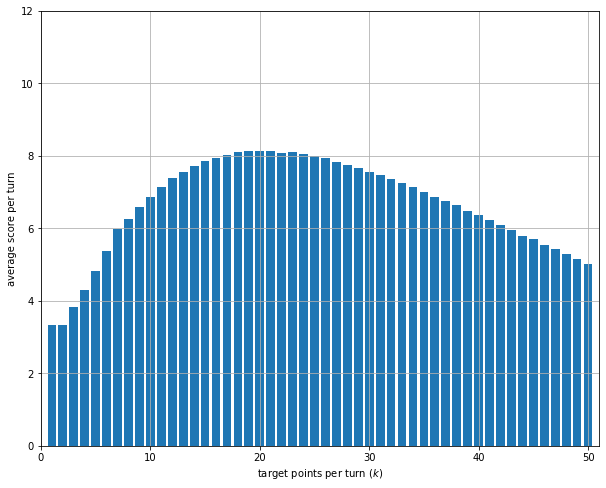
\includegraphics[width=0.7\linewidth]{figures/greedy_pig_sim}
	\end{center}
\caption{Distribution of expected number of points per turn.}
\label{fig:greedy_pig_sim}
\end{figure}
\end{solution}

\begin{question}
There are 60 chemical flasks in the laboratory, 6 of which are incorrectly labeled. What is the chance that if we randomly choose 5 flasks, exactly 3 of them will be labeled correctly ?

\noindent\textbf{Hint:} the probability is approximately 0.5 \%.
\end{question}

\cprotEnv\begin{solution}
\begin{ipython}
import random

flasks = ["C"]*54 + ["U"] * 6
random.seed(1)
trials = 1000
success = 0.

for _ in range(trials):
    draw = random.sample(flasks, 5)
    if draw.count("U") == 3:
        success += 1.

print ("Probability: {:.3f}%".format(success/float(trials)*100))
\end{ipython}
\begin{ioutput}
Probability: 0.499%
\end{ioutput}
\end{solution}

\begin{question}
Given the following historical series (1895-2020) find average September temperature in US and report the 99\% confidence interval of your measure.
\noindent
Input (temperatures are in Fahrenheit degrees): \href{https://raw.githubusercontent.com/matteosan1/finance_course/master/input_files/histo_temp.csv}{histo\_temp.csv}
\end{question}

\cprotEnv\begin{solution}
\begin{ipython}
from scipy.stats import norm
import numpy as np
import pandas as pd

# first download the input file
df = pd.read.csv("histo_temp.csv")
temperatures = df['T'].to_array()
alpha = 0.99

A = norm.ppf((1 + alpha)/2)
m, se = np.mean(temperatures), np.std(temperatures)
h = A*se/np.sqrt(len(temperatures))

print ("Avg temperature in September (US): {:.1f}".format(m))
print ("{:.1f}% confidence interval: +- {}".format(alpha*100, h))
\end{ipython}
\begin{ioutput}
Avg temperature in September (US): 65.1
99% confidence interval: +- 0.3
\end{ioutput}
\end{solution}

%\begin{question}
%Using the function \texttt{normal} of \texttt{numpy.random} simulate the price of a stock which evolves according to a log-normal stochastic process with a daily rate of return \(\mu=0.1\) and a volatility \(\sigma=0.15\) for 30 days.
%Also plot the price. Try to play with \(\mu\) and \(\sigma\) to see how the plot changes.
%\end{question}
%
%\cprotEnv\begin{solution}
%\begin{ipython}
%from numpy.random import normal, seed
%from matplotlib import pyplot as plt
%import math
%
%S = 100
%mu = 0.1
%sigma = 0.15
%T = 1
%seed(1)
%
%historical_series = [S]
%for i in range(30):
%    S = S * math.exp((mu - 0.5 * sigma * sigma) * T +
%        sigma * math.sqrt(T) * normal())
%    historical_series.append(S)
%
%plt.plot(range(31), historical_series)
%plt.xlabel("days")
%plt.ylabel("Price of stock X")
%plt.show()
%\end{ipython}
%
%\begin{figure}[!htb]
%\begin{center}
%  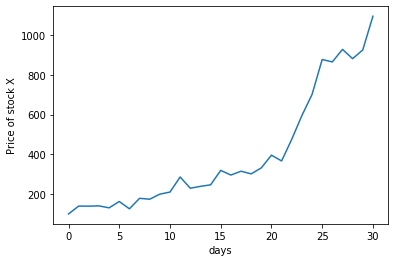
\includegraphics[width=0.7\linewidth]{figures/lesson6_solutions_5_0.png}
%\end{center}
%\caption{A realization of a stock price 30 days evolution.} 
%\end{figure}
%\end{solution}


\begin{thebibliography}{9}
\bibitem{cit:bernoulli_distribution}\href{https://en.wikipedia.org/wiki/Bernoulli_distribution}{\emph{Bernoulli Distribution Wikipedia}}
\end{thebibliography}









 % da riguardare
\chapter{Monte Carlo Simulation}
\label{cap:montecarlo}

The modern version of the Monte Carlo method dates back to the application of the first computers during the years 1940-45 with the purpose of computing neutron diffusion in atomic bombs.

The Monte Carlo approach was primarily promoted by physics researchers Stanislaw Ulam, Nicholas Metropolis and John von Neumann. They were well aware of the potential of such technique but it was only with the first electronic computer, the ENIAC, which was able to solve differential equations at a tremendous, and so far inconceivable, speed, that Monte Carlo method was eventually triggered.

The name Monte Carlo refers to the city in Monaco where Ulam's uncle used to indulge his gambling passion. The characteristics of randomness and the repetitive nature of many processes correspond with the games played in a casino. Note that the famous roulette wheel is one of the simplest mechanical devices to generate random variables.

Monte Carlo tools find their application mostly in cases where the inherent complexity of a problem makes the use of other techniques impossible or where no analytically tractable solution exists.
They are are widely used in many fields: Engineering, Physics, Computational biology, Computer graphics, Applied statistics and Artificial intelligence for games. It started to be en vogue in financial mathematics in the 1980s, particularly when the theories of the random walk of asset prices came up.

In this Chapter the Monte Carlo technique is reviewed with some applications.

\section{The Algorithm}
\label{whats-monte-carlo-simulation}

A Monte Carlo simulation is a mathematical technique that simulates the range of possible outcomes for an uncertain event. It relies on the assumption that many random samples mimic patterns of the total population.
Indeed it can be considered as the algorithmic translation of the expectation value, i.e.
$$
V_0 = \mathbb{E}^{\mathbb{Q}} \left[ D(0,T)\cdot X_T \right] \implies \mathbb{E} \text{ calculation} \iff \text{MC simulation}
$$
As we know

$$\mathbb{E}[g(X)] = \int_{-\infty}^{+\infty} g(x) f(x) \, dx$$
When the involved integral can't be analytically solved we can rely on the Strong Law of Big Numbers which states that: \textit{"sampling $N$ independent values $x_1, x_2, \dots, x_N$ from the distribution $f(x)$, the sample mean converges to the true value"}:

$$\lim_{N \to \infty} \frac{1}{N} \sum_{i=1}^{N} g(x_i) = \mathbb{E}[g(X)]$$

So the MC method is a direct application of the previous formula
\begin{enumerate}
	\item sampling: generate $N$ random scenarios/trajectories ($x_i$) complying the probability distribution of the system ($f(x)$).
	\item valuation: compute the function value (or payoff) $g(x_i)$ for each generated scenario.
	\item Monte Carlo estimator: compute the arithmetic mean of the previous calculations. This is the estimate of the expected value.
$$V_0 = e^{-rT} \, \mathbb{E}^{\mathbb{Q}}[X_T] \quad \approx \quad e^{-rT} \cdot \frac{1}{N} \sum_{i=1}^{N} X_T^{(i)}$$
where the MC approximates $\mathbb{E}^{\mathbb{Q}}$ of the payoff $X_T$ simulating $N$ plausible scenarios at time $T$.
\end{enumerate}

%The algorithm proceeds by simulating the process under study replacing every source of uncertainty by random numbers sampled from appropriate distributions (PDF).
%The results is re-calculated many times, using a different set of random numbers within the estimated range. This process generates many probable outcomes, which become more accurate as the number of inputs grows, i.e. law of large numbers.

The main advantage of the technique is that predictions are based on an estimated range of values instead of a fixed set and evolve randomly.
Note that depending upon the number of uncertainties and their ranges, a Monte Carlo simulation could involve thousands or even millions of recalculations before it is completed.
%
%Although they might vary from case to case, the general steps to a Monte Carlo simulation can be summarized as follows:
%
%\begin{itemize}
%\item Build the mathematical model.
%\item Determine an appropriate probability distribution (PDF) for each random variable and their range of variability $\Omega$.
%\item Run the random variables through the mathematical model to perform many iterations of the simulation.
%\item Aggregate the results, and determine mean and standard deviation to determine if the result is as expected. Visualize the results on a histogram.
%\end{itemize}

As an example imagine to simulate the results of rolling a die: the only variable is the die outcome, so $\Omega =1,2,3,4,5,6$ and the outcome probability is a uniform distribution (i.e. we are using a fair die and outcomes are equiprobable). Hence the simulation consists of sampling uniform distributed integers between 1 and 6.

\section{Pseudo-Random Numbers}
\label{pseudo-random-numbers}

The need of generating random inputs during a MC simulation requires large amounts of \emph{random numbers} to be generated. A random number is a "randomly chosen" number from a particular distribution.
Their use in Monte Carlo simulations spurred the development of \emph{pseudo-random number generators}. Nowadays every programming language has libraries that allow to produce huge series of random numbers. 

These series, which have very large periodicity (e.g. $2^{20000}$), are calculated by algorithms that take as input a \emph{seed} which determines them uniquely. \textbf{This means that choosing the same seed will produce the same set of numbers every time} (which is great for debugging purposes though).

In \texttt{python} there are two main ways to generate random numbers by using either \texttt{numpy.random} or \texttt{scipy.stats} modules. Among others, they have the following useful functions:
\begin{itemize}
\tightlist
\item \texttt{numpy.random.seed}: set the seed of the random number generator;
\item \texttt{numpy.random.uniform}, \texttt{scipy.stats.uniform.rvs}: returns a random number between 0 and 1 (with uniform probability);
\item \texttt{numpy.random.randint(min,\ max)}: returns an integer random number between \texttt{min} and \texttt{max} (with uniform probability);
\item \texttt{numpy.random.choice(aList,\ k=n, replace=True)}: samples n elements from the list \texttt{aList} with or without replacement.
\item \texttt{numpy.random.normal}, \texttt{scipy.stats.norm.rvs}: throws random numbers sampled from a normal distribution ($\mathcal{N}(0, 1)$).
\end{itemize}

\pythoncodenon{code/monte_carlo_1.py}
\begin{ioutput}
uniform distributed floats with seed 1
0.417022004702574, 0.7203244934421581
uniform distributed floats with seed 2
0.43599490214200376, 0.025926231827891333
uniform distributed floats with seed 1 again
0.417022004702574, 0.7203244934421581
random integer between 1-9: 6
choose two items among aList: ['c' 'd']
\end{ioutput}

\subsection{Sampling from a Distribution}

In probabilistic modeling and simulation, sampling from a given distribution means generating random numerical realizations governed by the mathematical laws of that distribution.
Rather than picking numbers arbitrarily, every draw respects the underlying probability density function: values associated with high probability occur frequently, while extreme or tail events appear only in proportion to their theoretical likelihood. 

For instance, sampling from a standard normal distribution $\mathcal{N}(0, 1)$ will yield numbers that cluster densely around zero, with large deviations becoming exponentially rare.

If we need to sample from a generic distribution it is convenient to use \texttt{scipy.stats}. Lots of useful distribution have been defined there, each with convenient methods e.g. \texttt{rvs(size=n)} allows to sample as many time as specified by the argument \texttt{size}. 

Below two examples which sample 50000 times from the discrete uniform distribution (\texttt{randint}) and from the normal distribution, the results are shown in  Fig.~\ref{fig:gauss_dist}.

\pythoncodenon{code/monte_carlo_2.py}

\begin{figure}[hb]
\centering
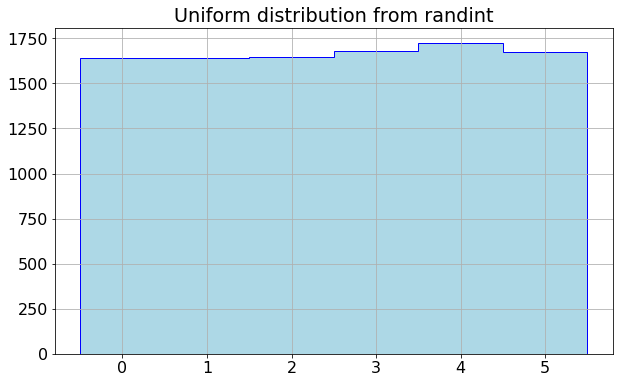
\includegraphics[width=0.45\textwidth]{figures/uniform}
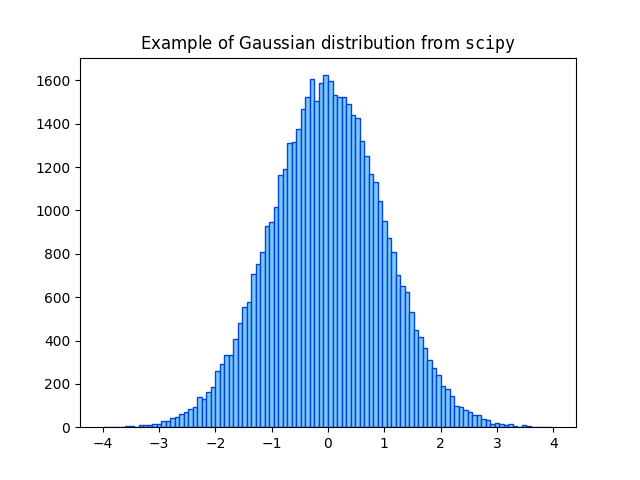
\includegraphics[width=0.45\textwidth]{figures/standard_normal}
\caption{Uniform distribution generated with \texttt{numpy.random.randint} function (left). Normal distribution generated with \texttt{scipy.stats.norm} function (right).}
\label{fig:gauss_dist}
\end{figure}

\section{Monte Carlo Simulation Examples}
\label{example-of-monte-carlo-simulation}

In this Section we go through some applications of the Monte Carlo method.

\subsection{Probability to Draw Two Kings From a Deck}

Imagine we would like to determine the probability of drawing consecutively two kings from a deck of 40 cards. At the beginning all the cards are available with 4 possible kings, so according to the frequentist approach~\ref{cap:bayes}, the probability to get the first king is $4/40=10\%$. Next, assuming we've got a king the first time, we are left with 39 cards and 3 kings only, so the probability to get the second one is $3/39=7.7\%$. Since we want both events to happen, the final probability is the product of the two:

\begin{equation*}
P_\textrm{two kings} = \frac{4}{40} \cdot \frac{3}{39} = \frac{1}{130} \approx 0.77\%
\end{equation*}

Let's now estimate the same probability with a MC simulation, following the steps outlined above.

\pythoncode{code/monte_carlo_3.py}

In this case the domain is a deck of cards; to simulate it we can define a list with the values of each card (actually we can create first the list of "cards" for a single suit and then "multiply" the list by four, see line 4). We pick up randomly, one million times, two cards from the virtual deck (line 8); for debugging purpose the first ten draws are printed on screen. Check if the card pair is \texttt{['K', 'K']} (line 11) and in case increase the counter of successes (line 12). Finally just print \texttt{successes/trials} which is the sought probability.
In the example we are going to set the seed to 1 to make it reproducible.

\begin{ioutput}
['3' '2']
['2' '3']
['7' '3']
['Q' '4']
['7' '5']
['5' 'J']
['4' 'K']
['K' '2']
['5' 'Q']
['A' 'J']

The probability to draw two kings is 0.0076
\end{ioutput}

The result is in agreement with the theoretical expectations, further considerations about this result in Section~\ref{sec:confidence_interval}.

\subsection{Determine $\pi$}
\label{determine-pi}

We know that $\pi\approx 3.141592653589793\ldots$ and in order to get an estimate through MC simulation of this famous constant a geometric approach can be considered. Imagine a circle of radius $r$ which is \emph{inscribed} in a square with side length $2r$, see Fig.~\ref{fig:circle_inscribed}.

\begin{figure}[htb]
\centering
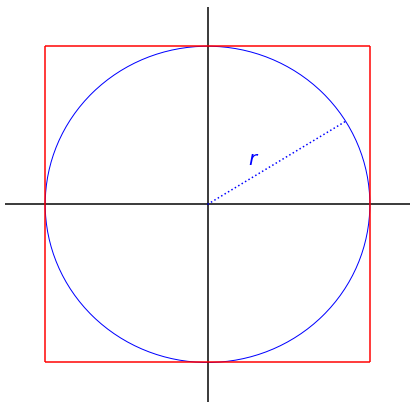
\includegraphics[width=0.5\textwidth]{figures/circle_inscribed}
\caption{A circle of radius $r$ inscribed in a square of side length $2r$.}
\label{fig:circle_inscribed}
\end{figure}

Computing the ratio of the two figure areas and solving for $\pi$ we get

\begin{equation}
\frac{\text{Area Circle}}{\text{Area Square}} = \frac{\pi r^2}{4r^2} = \frac{\pi}{4} \implies \pi \approx \cfrac{4\cdot\text{Area Circle}}{\text{Area Square}}
\end{equation}

The algorithm to approximate $\pi$ should then be

\begin{itemize}
\item select 2 random numbers, $x_1$ and $x_2$, from the interval $[-r,r]$; 
\item determine if the point $(x_1, x_2)$ lies within or on the circle, keeping track both of the total number of tested points and of those satisfying the condition $\sqrt{x_1^2 + x_2^2}\leq r$; 
\item approximate the ratio of the areas by the number of points within or on the circle divided by the total number of tested points; 
\item multiply the approximated area by 4 to get $\pi$.
\end{itemize}

\pythoncodenon{code/monte_carlo_4.py}
\begin{ioutput}
Approx. pi: 3.1524
\end{ioutput}

\section{Accuracy of Monte Carlo Simulation}
\label{sec:confidence_interval}

A general consideration that we can make is that the lower is the probability we try to estimate with MC the higher has to be the number of simulations. The result precision indeed depends on the amount of "successes" and if the success probability is small, many trials are needed. 
Imagine an event has a probability of 0.001 to happen. Running only 100 experiments we should see $100*0.001 \approx 0.1$ successful events, which means most likely no event will be recorded. 

\textbf{Note that this doesn't mean we can conclude the process has a 0 probability to happen, but just that I need to run a number of MC simulation of order of the thousands.} This can also be checked by playing with the number of simulations in the previous examples. We may run an entire simulation without getting two consecutive kings, nevertheless we cannot conclude there is zero probability of such event.

The only conclusion we can draw is that, despite its undoubted power, Monte Carlo simulation is not always the best approach to follow, especially for computationally heavy experiments. Many times indeed the simulation of a single experiment requires a lot of computing resources (and time) and it may not be practical to embark into quite a large simulation.

In the following example it is apparent how increasing the number of experiments the result precision increases. Fig.~\ref{fig:circle_approx} shows graphically the results with 100, 1000, 10000, 100000 and 1000000 simulations.

\pythoncodenon{code/monte_carlo_5.py}
\begin{ioutput}
pi=3.120000 0.0001s
pi=3.096000 0.0012s
pi=3.121200 0.0147s
pi=3.139560 0.1997s
pi=3.142136 1.0671s
\end{ioutput}

\begin{figure}[htb]
\centering
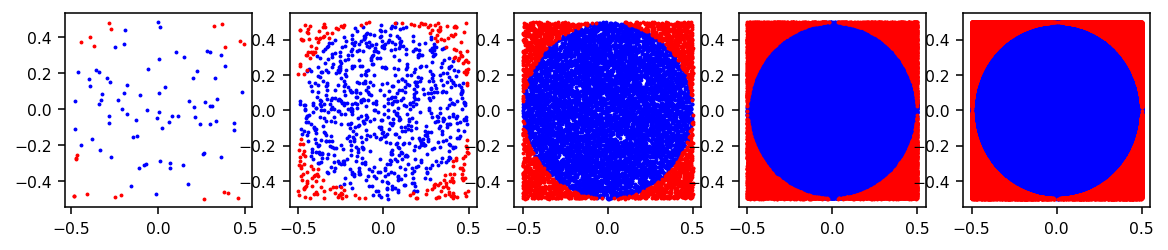
\includegraphics[width=1\textwidth]{figures/mc_vs_n_experiments}
\caption{Graphical representation of geometrical approximation of $\pi$. Results are reported for $N = 100, 1000, 10000, 100000, 1000000$ simulations. It is clear how the result improves with $N$.}
\label{fig:circle_approx}
\end{figure}
In this case the simulation is so simple that even in the larger case ($N=1000000$) the program runs for only about a second.

Now let's go back to the card example and imagine that you couldn't analytically compute the probability of getting two consecutive $'K'$ from the 40 cards deck. 

\pythoncodenon{code/monte_carlo_6.py}
\begin{ioutput}
0.0084
\end{ioutput}

What can be concluded from the result of this single MC experiment ? Unfortunately not much, butthe Central Limit Theorem~\cite{bib:central_limit} (CLT) come to rescue us. It states that if we have $X_1, X_2,\dots, X_n$ which are $n$ random samples from a distribution $X$ with true mean $\mu$ and variance $\sigma^{2}$, then with $n$ sufficiently large,

\begin{equation*} 
\mu_n = \cfrac{X_1 + X_2 +\ldots + X_n}{n} = \cfrac{1}{n}\sum_i^n X_i
\end{equation*}
has approximately a normal distribution $\mathcal{N}(\mu, \sigma^2/n)$.

This means that if one repeats the same MC experiment many times (changing the random number generator seed otherwise we are always repeating the \textbf{same} experiment) would obtain results normally distributed around the \textbf{true} value $\mu$. \emph{Also the best estimate $\mu_n$ of the unknown parameter $\mu$ is the mean of the MC experiment results.}

Another very important consequence of the CLT is that the error of our estimate $\mu_n$ is \emph{the standard deviation of the sample ($\sigma_{Y_i}$) divided by the square root of the sample size}. Indeed
\begin{equation*}
\begin{gathered}
\bar{X} = \cfrac{X_1 + X_2 +\ldots +X_n}{n}\\
\var(\bar{X}) = \var\left(\cfrac{X_1 + X_2 +\ldots +X_n}{n}\right)=\cfrac{\var(X_1)}{n^2}+\cfrac{\var(X_1)}{n^2}+\ldots+\cfrac{\var(X_n)}{n^2} = \\
=\cfrac{1}{n^2}[\sigma^2+\sigma^2+\ldots+\sigma^2] = \cfrac{\sigma^2}{n}
\end{gathered}
\end{equation*}

This is sometimes called the standard deviation of the sample mean (contrary to the standard deviation of a sample). Hence, the sample mean is much less volatile than the samples themselves. Consequently, the error reduces at the rate of 1 over the square root of the sample size. 

Suppose we first conduct a Monte Carlo simulation using $n_1$ experiments. The standard deviation of the unknown value estimate is $\cfrac{\sigma}{\sqrt{n_1}}$. Now if we would like to reduce that uncertainty by 50\% how much larger must the sample should be ? Let this new sample size be $n_2$. Then the standard deviation of the estimate becomes $\cfrac{\sigma}{\sqrt{n_2}}$.
Finally note that,
\begin{equation*}
  \cfrac{1}{2}\cfrac{\sigma}{\sqrt{n_1}}  = \cfrac{\sigma}{\sqrt{n_2}} \implies n_2 = 4 n_1
\end{equation*}
Thus, to achieve a 50\% increase in accuracy, we must \textbf{quadruple} the number of random experiments.











%No matter where you look, a bell curve is close by.
%
%Place a measuring cup in your backyard every time it rains and note the height of the water when it stops: Your data will conform to a bell curve. Record 100 people’s guesses at the number of jelly beans in a jar, and they’ll follow a bell curve. Measure enough women’s heights, men’s weights, SAT scores, marathon times — you’ll always get the same smooth, rounded hump that tapers at the edges.
%
%Why does the bell curve pop up in so many datasets?
%
%The answer boils down to the central limit theorem, a mathematical truth so powerful that it often strikes newcomers as impossible, like a magic trick of nature. “The central limit theorem is pretty amazing because it is so unintuitive and surprising,” said Daniela Witten (opens a new tab), a biostatistician at the University of Washington. Through it, the most random, unimaginable chaos can lead to striking predictability.
%
%It’s now a pillar on which much of modern empirical science rests. Almost every time a scientist uses measurements to infer something about the world, the central limit theorem is buried somewhere in the methods. Without it, it would be hard for science to say anything, with any confidence, about anything.
%
%
%
%Perhaps it shouldn’t come as a surprise that the push to find regularity in randomness came from the study of gambling.
%Abraham de Moivre made early mathematical investigations into games of chance.
%
%Flipping a coin, rolling a die, and drawing a card from a deck are random actions, with every outcome equally likely. What de Moivre realized is that when you combine many random actions, the result follows a reliable pattern.
%
%Flip a coin 100 times and count how often it comes up heads. It’ll be somewhere around 50, but not very precisely. Play this game 10 times, and you may get 10 different counts.
%
%Now imagine playing the game 1 million times. The bulk of the outcomes will be close to 50. You’ll almost never get under 10 heads or over 90. If you make a graph of how many times you see each number between zero and 100, you’ll see that classic bell shape, with 50 at the center. The more times you play the game, the smoother and clearer the bell will become.
%
%De Moivre figured out the exact shape of this bell, which came to be called the normal distribution. It told him, without his having to actually play the game, how likely different outcomes were. For instance, the probability of getting between 45 and 55 heads is about 68%.
%
%Let’s take an example slightly more complex than coin flips: dice rolls. Every roll of a die has six equally likely outcomes. If you repeatedly roll the die and tally the results, you’ll get a chart that looks flat — you’re bound to see about as many rolls of 1 as you do 2 or 4 or 6.
%
%Now roll that die 10 times and take the average. You’re likely to get somewhere around 3.5. Repeat the experiment many more times and graph up all the results. You’ll get a bell curve that peaks at 3.5, with a precisely defined structure on either side.
%
%That’s the magic of the central limit theorem. You started with a distribution of possible outcomes that has no structure at all — equal chances of rolling 1 through 6. But by taking an average of multiple measurements, then repeating that process over and over, you get a precise, predictable, mathematical structure: the bell curve.
%
%Laplace distilled this structure into a simple formula, the one that would later be known as the central limit theorem. No matter how irregular a random process is, even if it’s impossible to model, the average of many outcomes has the distribution that it describes. “It’s really powerful, because it means we don’t need to actually care what is the distribution of the things that got averaged,” Witten said. “All that matters is that the average itself is going to follow a normal distribution.”
%
%Averaging might seem like something it takes a human to do, but the central limit theorem applies invisibly to all kinds of things we can observe in the world, like human heights. “Somebody’s height might depend on their dad’s height, and their mom’s height, and their genetics, and their nutrition, and all these little effects that add up,” said Jeffrey Rosenthal (opens a new tab), a statistician at the University of Toronto. Those effects are unrelated to each other (generally, your dad’s height has nothing to do with the food you eat). “It’s kind of like averaging a bunch of little effects,” said Rosenthal, which is why height approximately follows a normal distribution.
%
%The theorem also gives statisticians the power to tell when something fishy is happening. Say you’re sipping coffee at Old Slaughter’s when a patron hands you a coin and bets that you can’t get 45 heads in 100 flips. You try, and only get 20. How can you tell whether he gave you a trick coin and the process is not as random as it ought to be? Thanks to the central limit theorem, you know that the numbers up to 20 only cover 0.15% of the bell, so there’s only a 0.15% chance a fair coin would give such a bad result. You’re almost certainly being had.
%
%That’s the true power of Laplace’s formula. He knew that averaging over any process gives you a bell curve, which lets you say something about that process, without knowing anything deeper about how it works.
%
%Despite its centrality to modern science, the central limit theorem has limits of its own. It only works when you’re combining many samples, and those samples need to be independent. If they’re not — for example, if you only run a national presidential poll in a single small town in Maine — repeating the experiment won’t get you closer to the expected bell curve.


\subsection{Central Limit Theorem in the Kings Example}

We can check the Central Limit Theorem by repeating many times the virtual deck MC experiment and see how the distribution of $\mu_n$ behaves.

\pythoncodenon{code/monte_carlo_7.py}
\begin{ioutput}
mu_true: 0.007692
mu: 0.007640 +- 0.000151
\end{ioutput}

Looking at Fig.~\ref{fig:repeated_MC} it is clear that the various results are distributed as a Gaussian (in this example the distribution is still a bit asymmetric but it will eventually become Gaussian running more simulations). Also playing with the parameter experiments it easy to see how the precision of the estimate increase always staying within the assigned error interval.

\begin{figure}[htb]
\centering
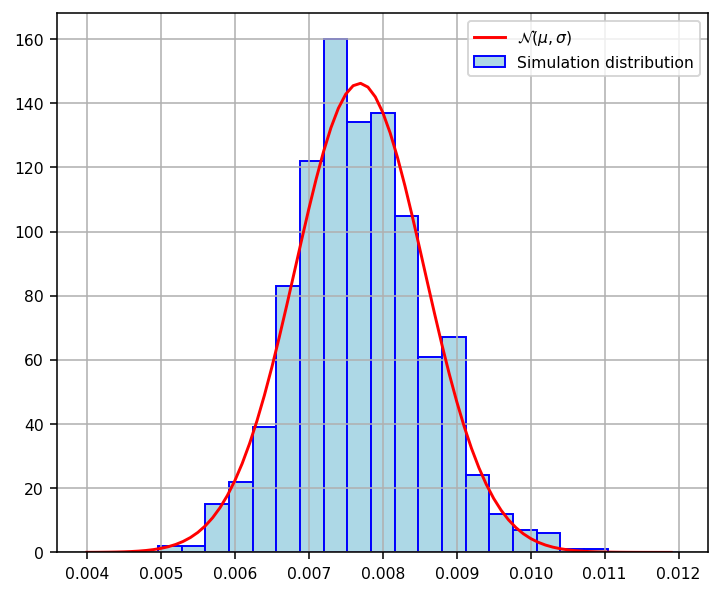
\includegraphics[width=0.7\textwidth]{figures/experiment_distribution}
\caption{Distribution of the results of 1000 experiments.}
\label{fig:repeated_MC}
\end{figure}

\subsection{Confidence Interval}

From the Central Limit Theorem we know that: 

\begin{equation}
\mu_n - \mu \approx \mathcal{N}(0, \sigma^2/n)
\end{equation}
Remembering the definition of quantiles~\ref{sec:quantile-function} it is then possible to define an interval such that there is a certain probability to find $\mu$ in there. Referring to Fig.~\ref{fig:confidence_interval} we can write:

\begin{equation}
P\left(\mu_n - 1.96\frac{\sigma}{\sqrt{n}}\le \mu \le \mu_n + 1.96\frac{\sigma}{\sqrt{n}}\right) = 0.95
\end{equation}
(which corresponds to the pink area).

\begin{figure}[htb]
\centering
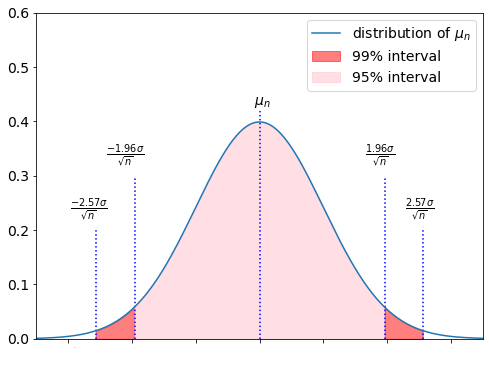
\includegraphics[width=0.7\textwidth]{figures/confidence_interval}
\caption{Confidence interval for a MC experiment.}
\label{fig:confidence_interval}
\end{figure}

This interval is called \textbf{95\% confidence interval} because it covers 95\% of the total area under the Gaussian. It can be interpreted like the following: if you repeat many times a simulation, the fraction of calculated confidence intervals that contains the true parameter $\mu$ would tend toward 95\%.

The most commonly used intervals are 99\% and 95\% confidence level and are respectively defined as \(\pm \cfrac{2.57\sigma}{\sqrt{n}}\) and \(\pm \cfrac{1.96\sigma}{\sqrt{n}}\).

To construct an interval with a custom confidence level $\alpha$, we have to find a number $A$ such that
\begin{equation}
\Phi(A) = 1 - \frac{1-\alpha}{2}\quad\implies\quad A = \Phi^{-1}\left(\cfrac{1+\alpha}{2}\right)
\label{for:A}
\end{equation}
then the $\alpha$-confidence interval guarantees
\begin{equation}
P(\mu - A\sigma \le X \le \mu+ A\sigma) = \alpha 
\end{equation}

Below an example of how to compute a confidence level in \texttt{python} given a set of simulation results (the inverse of the Gaussian CDF $\Phi^{-1}$, used in Eq.~\ref{for:A}, is computed with the method \texttt{norm.ppf()}, see Section~\ref{sec:quantile-function}).

\pythoncodenon{code/monte_carlo_8.py}
\begin{ioutput}
95% confidence int.: 4.437 +- 0.812
\end{ioutput}

%\section{Integration by Monte Carlo}
%\label{sec:integration}
%
%\begin{finmarkets}
%Function integration in \texttt{python} can be performed using \texttt{scipy.integrate.quad}. This method takes in input: the function to integrate, the integration limits and, if needed, optional arguments for the integrand (see Section~\ref{sec:kwargs_args}). Since it is a numerical integration the result will be a tuple with the actual result and its associated error.
%
%For example imagine to integrate
%\begin{equation*}
%f(x) = \int_{0}^{\infty}\frac{e^{-x}}{\left(a + (x-1)^2\right)}~dx
%\end{equation*}
%for $a=3$.
%
%\pythoncodebox{code/monte_carlo_7.py}
%\begin{ioutput}
%(0.2802620835548487, 1.5887625490132047e-09)
%\end{ioutput}
%\end{finmarkets}
%
%Sometimes it may be useful to calculate the approximate result of an integral of a function $f$ through Monte Carlo simulation. The technique relies on the fact that the average of $f$ calculated in the integration interval can be expressed as
%
%\begin{equation}
%<f(x)> = \frac{1}{b-a} \int_{a}^{b} f(x) \,dx
%\end{equation}
%Rearranging the terms
%\begin{equation}
%\int_{a}^{b} f(x) \,dx = 
%(b-a) <f(x)> \approx (b-a) \frac{1}{N} \sum_{i=1}^{N} f(x_i)
%\end{equation}
%Then the integral can be computed by sampling values of $x$ from a uniform distribution between $[a,b]$, average the evaluations of $f(x)$ and then multiplying the result by $(b-a)$.
%
%Considering the previous integral
%
%\pythoncodenon{code/monte_carlo_8.py}
%\begin{ioutput}
%0.28061306413101306
%\end{ioutput} 
% 
%Although there are various improvements that can be added to our simple MC implementation, the result that we obtained is in good agreement with the one from the \texttt{python} implementation.  

\section*{Exercises}
\cprotEnv\begin{question}
Using the function \texttt{randint} of the module \texttt{random} make a Monte Carlo simulation of rolling three dice to check the probability of getting the same values on the three of them.
From probability theory you should expect:

\begin{equation*}
P_{d1=d2=d3} = \frac{1}{6}\cdot\frac{1}{6}\cdot\frac{1}{6}\cdot 6 = \frac{1}{36} = 0.0278
\end{equation*}
\end{question}

\cprotEnv\begin{solution}
\begin{ipython}
from random import seed, randint

seed(1)
trials = 10000000
success = 0

for _ in range(trials):
    d1, d2, d3 = randint(1, 6), randint(1, 6), randint(1, 6)
    if d1 == d2 and d2 == d3:
        success += 1

print ("The probability to get three equal dice is {:.4f}".format(success/trials))
\end{ipython}
\begin{ioutput}
The probability to get three equal dice is 0.0278
\end{ioutput}
\end{solution}

\begin{question}
Two fair dice are rolled, find the probability that their sum is:
\begin{enumerate}[start=1]
\item equal to 1;
\item equal to 4;
\item less than 13.
\end{enumerate}
	
\noindent\textbf{Hint:} the possible combinations of the outcomes of two dice are 36 (to realize it you can simply think that for each one of the six faces of the first die you have six possible faces of the second hence $6\cdot 6=36$). It is not possible to get 1 since the dice have no face with 0 so the first probability should come out 0. The sum of the two dice is always less than 13 (the maximum is 12\ldots) so the answer to point 3 is 1. We can get a sum of 4 in 3 cases (1-3, 3-1 or 2-2) so the expected probability is $3/36=1/12=0.0833$
\end{question}

\cprotEnv\begin{solution}
\begin{ipython}
import random

random.seed(1)
successes = {"=1":0.0, "=4":0.0, "<13":0.0}
trials = 100000

for _ in range(trials):
    d1 = random.randint(1, 6)
    d2 = random.randint(1, 6)

    if (d1 + d2) == 1:
        successes["=0"] += 1.0
    if (d1 + d2) == 4:
        successes["=4"] += 1.0
    if (d1 + d2) < 13:
        successes["<13"] += 1.0

for k,v in successes.items():
    print ("P({}): {:.3f}".format(k, v/trials))
\end{ipython}
\begin{ioutput}
P(=1): 0.000
P(=4): 0.084
P(<13): 1.000
\end{ioutput}
\end{solution}

\begin{question}
Let’s assume we have a process constructed from 3 stages $(X1, X2, X3)$. Each one has an average duration (5, 10 and 15 minutes) which vary following the normal distribution and we know their variance (all 1 minute).

We want to know what is the probability that the process will exceed 34 minutes?
\end{question}

\cprotEnv\begin{solution}
We know all the individual components so let’s define the relationship between them:

\begin{equation*}
Y = X_1 + X_2 + X_3
\end{equation*}

The single-component can be represented with a short function
\begin{ipython}
import numpy as np

def mc_normal(mean, std_dev, samples):
    results = []
    for _ in range(samples):
        results.append(np.random.normal(mean, std_dev))
    return np.array(results)
\end{ipython}

The Monte Carlo simulation code shown below uses this function as a basic block. The number of iterations for this use case is set at 10000 but you can change it. The last section of a code checks the probability of exceeding the limit of 34 minutes. Note how this can be computed when using \texttt{numpy.array}: \texttt{total > upper\_limit} returns an array with 1 or 0 depending on each element of total is greater then the limit or not; the element sum of the new array gives the number of "successes". 

\begin{ipython}
s = 100000

upper_limit = 34

component_1 = mc_normal(5,1,s)
component_2 = mc_normal(10,1,s)
component_3 = mc_normal(15,1,s)

total = component_1 + component_2 + component_3
probability = np.sum(total > upper_limit)/len(total)*100
print("Probability of exceeding the time limit: ", round(probability, 3), "%")
\end{ipython}

After running the following code we get an answer but it will vary every time you run the code:
\begin{ioutput}
Probability of exceeding the time limit:  1.016 %
\end{ioutput}

Now we can plot the histogram of the estimated parameter (time). We clearly see it follows the normal distribution.

\begin{figure}[htbp]
	\begin{center}
		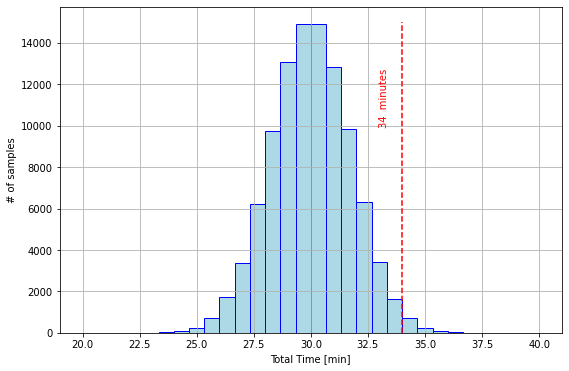
\includegraphics[width=0.7\linewidth]{figures/mc_processes}
	\end{center}
	\caption{Distribution of estimated times for the total process.}
	\label{fig:mc_processes}
\end{figure}
\end{solution}

\begin{question}
Write a Greedy Pig (see Ex.~\ref{ex:greedy_pig}) Monte Carlo simulation for a player aiming at $k$ points each turn (i.e. the turn simulation goes on until a 1 is rolled or $k$ points are reached).
Plot the distribution of the average number of points as a function of $k$.
\end{question}
\cprotEnv\begin{solution}
\begin{ipython}
import numpy as np
from random import randint

k = 20
sim = 1000000
points = [0 for _ in range(51)]

for s in range(sim):
    for k in range(1, 51):
        p = 0 
        while p < k:
            d = randint(1, 6)
            if d == 1:
                p = 0
                break
            else:
                p += d

points[k] += p
points = np.array(points)/sim
\end{ipython}

Figure~\ref{fig:greedy_pig_sim} confirms what has been already found in a previous Exercise. Aiming at 20 points per turn is the strategy that maximizes the number of expected points.

\begin{figure}[htbp]
	\begin{center}
		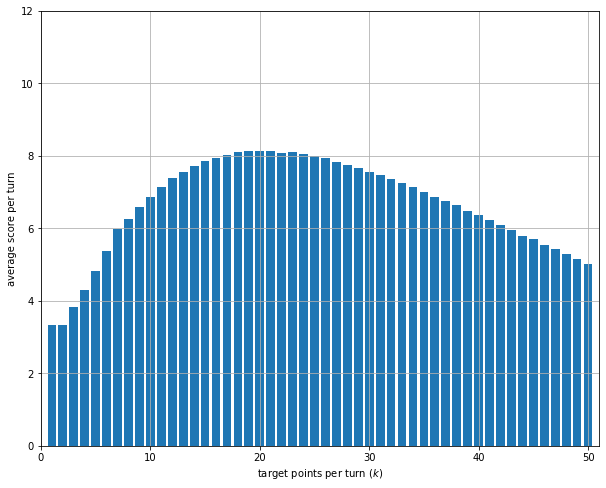
\includegraphics[width=0.7\linewidth]{figures/greedy_pig_sim}
	\end{center}
\caption{Distribution of expected number of points per turn.}
\label{fig:greedy_pig_sim}
\end{figure}
\end{solution}

\begin{question}
There are 60 chemical flasks in the laboratory, 6 of which are incorrectly labeled. What is the chance that if we randomly choose 5 flasks, exactly 3 of them will be labeled correctly ?

\noindent\textbf{Hint:} the probability is approximately 0.5 \%.
\end{question}

\cprotEnv\begin{solution}
\begin{ipython}
import random

flasks = ["C"]*54 + ["U"] * 6
random.seed(1)
trials = 1000
success = 0.

for _ in range(trials):
    draw = random.sample(flasks, 5)
    if draw.count("U") == 3:
        success += 1.

print ("Probability: {:.3f}%".format(success/float(trials)*100))
\end{ipython}
\begin{ioutput}
Probability: 0.499%
\end{ioutput}
\end{solution}

\begin{question}
Given the following historical series (1895-2020) find average September temperature in US and report the 99\% confidence interval of your measure.
\noindent
Input (temperatures are in Fahrenheit degrees): \href{https://raw.githubusercontent.com/matteosan1/finance_course/master/input_files/histo_temp.csv}{histo\_temp.csv}
\end{question}

\cprotEnv\begin{solution}
\begin{ipython}
from scipy.stats import norm
import numpy as np
import pandas as pd

# first download the input file
df = pd.read.csv("histo_temp.csv")
temperatures = df['T'].to_array()
alpha = 0.99

A = norm.ppf((1 + alpha)/2)
m, se = np.mean(temperatures), np.std(temperatures)
h = A*se/np.sqrt(len(temperatures))

print ("Avg temperature in September (US): {:.1f}".format(m))
print ("{:.1f}% confidence interval: +- {}".format(alpha*100, h))
\end{ipython}
\begin{ioutput}
Avg temperature in September (US): 65.1
99% confidence interval: +- 0.3
\end{ioutput}
\end{solution}

%\begin{question}
%Using the function \texttt{normal} of \texttt{numpy.random} simulate the price of a stock which evolves according to a log-normal stochastic process with a daily rate of return \(\mu=0.1\) and a volatility \(\sigma=0.15\) for 30 days.
%Also plot the price. Try to play with \(\mu\) and \(\sigma\) to see how the plot changes.
%\end{question}
%
%\cprotEnv\begin{solution}
%\begin{ipython}
%from numpy.random import normal, seed
%from matplotlib import pyplot as plt
%import math
%
%S = 100
%mu = 0.1
%sigma = 0.15
%T = 1
%seed(1)
%
%historical_series = [S]
%for i in range(30):
%    S = S * math.exp((mu - 0.5 * sigma * sigma) * T +
%        sigma * math.sqrt(T) * normal())
%    historical_series.append(S)
%
%plt.plot(range(31), historical_series)
%plt.xlabel("days")
%plt.ylabel("Price of stock X")
%plt.show()
%\end{ipython}
%
%\begin{figure}[!htb]
%\begin{center}
%  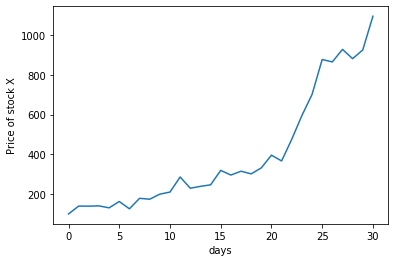
\includegraphics[width=0.7\linewidth]{figures/lesson6_solutions_5_0.png}
%\end{center}
%\caption{A realization of a stock price 30 days evolution.} 
%\end{figure}
%\end{solution}











\chapter{Stochastic Processes}

%In financial engineering, simulation tools have been increasingly gaining importance due to both the continuous enhancement of computational efficiency and the development of very complex financial instruments, e.g. derivatives. 

\section{Markov Process}
 
A \emph{stochastic or random process} can be defined as a collection of random variables indexed by some mathematical set (usually time), meaning that each random variable of the stochastic process is uniquely associated with an element in that set. Figure~\ref{fig:random_process} shows a graphical representation of a random process.

\begin{figure}[htb]
\centering
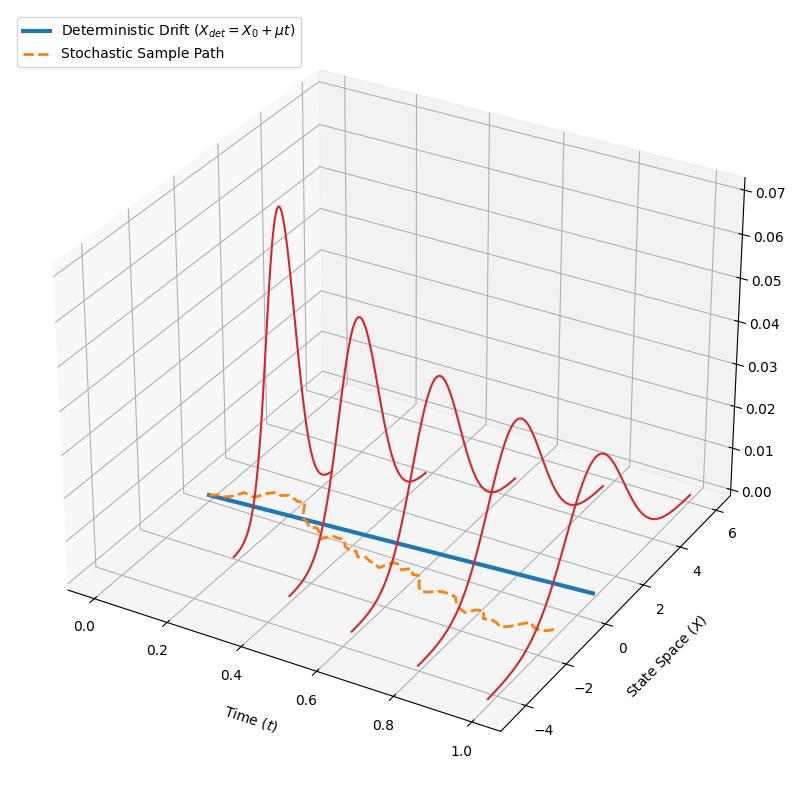
\includegraphics[width=0.55\textwidth]{figures/brownian_process}
\caption{Representation of a random process $X(t)$. Notice that, at each time $t$, the corresponding random variable has a probability distribution whose $\sigma$ increase with $t$.}
\label{fig:random_process}
\end{figure}

A model of the dynamics of asset prices is a nice example of a \emph{Markov process} since it must reflect the stochastic nature of price movements. Markov processes are a particular type of stochastic process without any history: past values and the way the present has emerged from the past are irrelevant, in other words they are memory-less.

\subsubsection{Wiener Process}
The \emph{Wiener process} ($W$) or elementary Brownian motion is the simplest example of Markov process. It is characterized by stationary and independent increments that are normally distributed. Those can be expressed as

\begin{equation}
\Delta W = Z\sqrt{\Delta t}
\end{equation}
where $Z\approx \mathcal{N}(0, 1)$ represents the standard normal Gaussian. 
The mean of $\Delta W$ is zero and its variance is $\Delta t$, which means the standard deviation grows with the square root of time. It follows that $W(t)\approx \mathcal{N}(0, t)$ because each $\Delta W$ is independently distributed like a standard Gaussian. Figure~\ref{fig:wiener_process} shows two realizations of Wiener process.

\begin{figure}[htb]
	\centering
	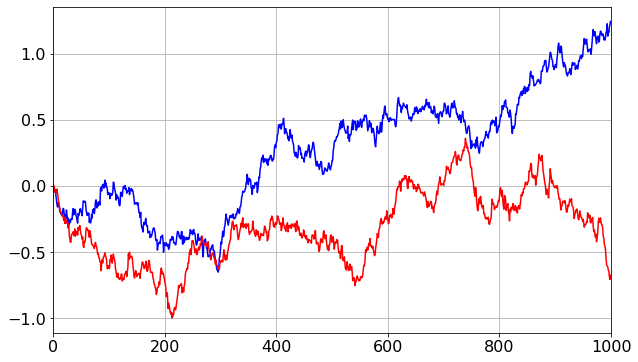
\includegraphics[width=0.7\linewidth]{figures/wiener_process.png}
	\caption{Two Wiener process realizations.}
	\label{fig:wiener_process}
\end{figure}

\subsubsection{It$\hat{o}$ Processes} 
An It$\hat{o}$ process ($X$) increments instead satisfy the following \emph{stochastic differential equation} (SDE) 
\begin{equation}
dX(t) = \mu(t, X(t)) dt + \sigma(t, X(t)) dW(t)
\end{equation}
A stochastic differential equation has one or more of the terms which are stochastic, resulting in a solution which is also a stochastic process.

In the special case where both \emph{drift} $\mu$ and the diffusion coefficient $\sigma$ are deterministic and independent of time $t$ and $X$, the process $X(t)$ is called an \emph{arithmetic Brownian motion}. The corresponding SDE is
\begin{equation}
dX(t) = \mu dt + \sigma dW(t) = \mu dt + \sigma \sqrt{t} \mathcal{N}(0,1) 
\end{equation}
thus $X(t)\approx \mathcal{N}(\mu t, \sigma^2 t)$.

Figure~\ref{fig:random_process} shows how the stochastic term grows linearly with time in an arithmetic Brownian motion.
Since such a process can take negative values is apparently unsuitable for simulating asset prices. These are rather assumed to follow a \emph{geometric Brownian motion} (GBM) instead, which is going to be described in the next Section. 

\section{Geometric Brownian Motion}
\label{derivation-of-log-normal-stochastic-differential-equation}

A stock price ($S(t)$ or $S_t$) deviates from a steady state as a result of random fluctuations given by the trades. Its relative change during a period $dt$ can be decomposed into two parts

\begin{itemize}
\tightlist
\item \emph{deterministic part}: represented by the expected return from the stock held during $dt$ and which can be expressed as $\mu S_tdt$ (with $\mu$ being the expected rate of return);
\item \emph{stochastic part}: reflects the random changes of the market (e.g. as a response to external effects such as unexpected news). A reasonable assumption is to consider this contribution proportional to the stock so $\sigma S_t dW_t$, where $dW_t$ is a Wiener process.
\end{itemize}
Putting the two contributions together the resulting SDE is:

\begin{equation}
dS_t = \mu S_t dt + \sigma S_t dW_t
\label{eq:differential}
\end{equation}
or dividing by $S_t$
\begin{equation}
\cfrac{dS_t}{S_t} = d\textrm{log}(S_t) = \mu dt + \sigma dW_t
\label{eq:differential_relative}
\end{equation}

The solution of Eq.~\ref{eq:differential_relative} can be derived by applying It$\hat{o}$'s formula~\cite{bib:ito_lemma}, which, roughly speaking, says that the derivative of a stochastic function with respect to time has an additional \emph{deterministic} term compared to the usual derivative we know from standard calculus. More formally it states that for any given continuous and differentiable function $G(S, t)$ where $S$ satisfies $dS=a\cdot dt +b\cdot dW_t$ holds

\begin{equation}
dG = \left(a\cfrac{\partial G}{\partial S} + \cfrac{\partial G}{\partial t} + \cfrac{1}{2}b^2\cfrac{\partial^2 G}{\partial S^2} \right)dt + b \cfrac{\partial G}{\partial S}dW
\label{eq:itos_lemma}
\end{equation}
which is essentially an extension of the \emph{Taylor series} expansion applicable to stochastic functions.

\begin{attention}
\subsubsection{Derivation of It$\hat{o}$'s Lemma}
Assume $X_t$ is a process that satisfies the stochastic differential equation
\begin{equation*}	
dX_{t}=\mu_{t}\,dt+\sigma_{t}\,dW_{t}
\end{equation*}
If $f(x, t)$ is a twice-differentiable scalar function, its expansion in a Taylor series is
	
\begin{equation*}
df={\cfrac {\partial f}{\partial t}}\,dt+{\cfrac {\partial f}{\partial x}}\,dx+{\cfrac {1}{2}}{\cfrac {\partial ^{2}f}{\partial x^{2}}}\,dx^{2}+\cdots 
\end{equation*}

Substituting $X_t$ for $x$ and therefore $\mu_t dt + \sigma_t dW_t$ for `$dx$ gives
	
\begin{equation*}
df={\cfrac {\partial f}{\partial t}}\,dt+{\cfrac {\partial f}{\partial x}}(\mu _{t}\,dt+\sigma _{t}\,dW_{t})+{\cfrac {1}{2}}{\cfrac {\partial ^{2}f}{\partial x^{2}}}\left(\mu _{t}^{2}\,dt^{2}+2\mu _{t}\sigma _{t}\,dt\,dW_{t}+\sigma _{t}^{2}\,dW_{t}^{2}\right)+\cdots 
\end{equation*}

In the limit $dt\rightarrow 0$, the terms $dt^2$ and $dt\cdot dW_t$ tend to zero faster than $dW_t^2$, which is $O(dt)$. Neglecting those terms, substituting $dt$ for $dW_t^2$ (it is a Wiener process), and collecting the $dt$ and $dW_t$ terms, we obtain
	
\begin{equation*}
df=\left({\cfrac {\partial f}{\partial t}}+\mu _{t}{\cfrac {\partial f}{\partial x}}+{\cfrac {\sigma _{t}^{2}}{2}}{\cfrac {\partial ^{2}f}{\partial x^{2}}}\right)dt+\sigma _{t}{\cfrac {\partial f}{\partial x}}\,dW_{t}
\end{equation*}
\end{attention}

If we set $G = \textrm{log}(S_t)$ we can compute the derivatives:

\begin{equation}
\begin{gathered}
\cfrac{\partial G}{\partial S} = \cfrac{1}{S_t}\\[5pt]
\cfrac{\partial G}{\partial t} = 0\\[5pt]
\cfrac{\partial^2 G}{\partial S^2} = -\cfrac{1}{S_t^{2}}
\end{gathered}
\end{equation}
Substituting back into Eq.~\ref{eq:itos_lemma} and taking the values of $a$ and $b$ from Eq.~\ref{eq:differential} we get:

\begin{equation}
\begin{gathered}
d(\textrm{log} S_t) = \left(\mu S_t \cfrac{1}{S_t} + \cfrac{1}{2}\sigma^2 S_t^2 (-\cfrac{1}{S_t^2})\right)dt + \sigma Z\sqrt{dt}\\[5pt]
\textrm{log} (S_t) - \textrm{log} (S_{t-1}) = \textrm{log} \cfrac{S_t}{S_{t-1}} = \left(\mu - \cfrac{1}{2}\sigma^2\right)dt + \sigma Z\sqrt{dt}\\[5pt]
S_t = S_{t-1}\cdot\textrm{exp}\left[\left(\mu - \cfrac{1}{2}\sigma^2\right)dt + \sigma Z\sqrt{dt}\right] \implies S_t = S_0 \prod_{i=0}^{t-1} dS_i 
\end{gathered}
\label{eq:gbm_solution}
\end{equation}
As can be seen from the second of Eqs.~\ref{eq:gbm_solution} the variation in $\textrm{log} S_t$ has a constant (the \emph{drift} $\mu - \frac{1}{2}\sigma^2$) plus a Gaussian distributed random variable (remember that $Z$ is $\mathcal{N}(0,1)$). Therefore $\textrm{log} S_t$ at some time $T$ is 

\begin{equation}
\textrm{log}S_t \approx\mathcal{N}\left[\left(\mu-\frac{\sigma^2}{2}\right)T, \sigma^2 T\right]
\end{equation}
A random variable like $S_t$ whose logarithm is normally distributed is said to be \emph{log-normal}. 

It follows that the stock price at time $T$, given today's price, is log-normally distributed. One of the most important properties of a log-normal distribution is to be positive definite and that's why it is a good characteristic for stock prices, see Figure~\ref{fig:log_normal}. 

%It is possible to check how a log-normal PDF looks like with the following lines of code. Figure~\ref{fig:log_normal} shows the resulting distribution.
%
%\begin{ipythonnon}
%from matplotlib import pyplot as plt
%from scipy.stats import lognorm
%from numpy import arange
%
%x = arange(-1, 5, 0.01)
%plt.plot(x, lognorm.pdf(x, 1), color='blue', label='Log-normal PDF')
%plt.grid(True)
%plt.xlim(-1, 5)
%plt.ylim(0, 0.7)
%plt.legend()
%plt.show()
%\end{ipythonnon}

\begin{figure}[htb]
\centering
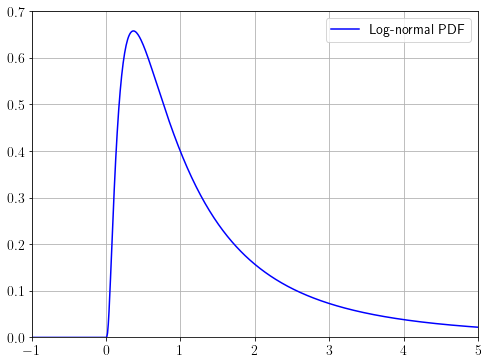
\includegraphics[width=0.5\textwidth]{figures/log_normal}
\caption{Log-normal PDF, it is apparent how such distribution doesn't have non-zero probabilities for $x<0$.}
\label{fig:log_normal}
\end{figure}

Actually this result was expected, in fact looking at the initial $dS$ expression (Eq.~\ref{eq:differential}) we had:

\begin{equation}
dS_t = \mu S_tdt + \sigma S_t dW_t
\end{equation}
which shows that the closer $S_t$ is to 0, the smaller is its variation $dS$, so it will never go negative.

\section {Simulating Stochastic Differential Equations}
Several kind of numerical schemes can be used to simulate SDEs, however we restrict our discussion to the two most fundamental ones, the \emph{Euler scheme} and the \emph{Milstein scheme}. 

As a starting point for both methods, consider an SDE of the form
\begin{equation}
dX(t) = \mu(t, X(t))dt + \sigma(t, X(t)) dW (t)
\label{eq:sde}
\end{equation}

Suppose that we are interested in simulating values of $X(T)$ without knowing an explicit solution of Eq.~\ref{eq:sde}. 

\subsection{Euler Scheme}
Consider $X$ at a time $t_i$, the value at $t_{i+1} = t_i +\Delta t$ can be determined directly applying the SDE of Eq.~\ref{eq:sde} sampling from the standard normal $Z_i \approx \mathcal{N}(0,1)$

\begin{equation}
X(t_{i+1}) = X(t_i) + \mu(t_i , X(t_i))\Delta t + \sigma(t_i , X(t_i))\sqrt{\Delta t}Z_{i+1}
\label{eq:euler_scheme}
\end{equation}
The process is discretized at constant time steps and the implementation is quite straightforward, at least if drift and diffusion are easy to evaluate.

\begin{attention}
\subsection{Milstein Scheme}
The accuracy of numerical solutions of ordinary differential equations may be improved by simple Taylor expansions. A very similar strategy also applies to SDEs. Yet it is crucial to account for the rules of It$\hat{o}$ calculus in order to maintain consistency.

Inspecting the Euler scheme from the perspective of Taylor expansions leads to a possible inconsistency: such an approximation expands the drift to the order $O(\Delta t)$ but the diffusion term only to $O(\sqrt{\Delta t})$. This suggests to focus on the latter to improve the Euler scheme.

The \textit{Milstein scheme} is defined as an ordinary Euler scheme where the next order terms of the It$\hat{o}$ expansion of Equation~\ref{eq:sde} are included. This eventually leads to

\begin{equation}
\begin{aligned}
X(t_{i+1})= X(t_i) &+ \mu(t_i, X(t_i))\Delta t+\sigma(t_i,X(t_i))\sqrt{\Delta t}Z_{i+1} \\
&+\cfrac{1}{2}\sigma'(t_i ,X(t_i))\sigma (t_i ,X(t_i))\Delta t(Z^2_{i+1} -1)
\end{aligned}
\end{equation}

The Milstein approximation thus simply involves the addition of a term to the Euler scheme so that both the drift and diffusion terms are expanded to $O(\Delta t)$ to eliminate the inconsistency. 

However, the question remains whether it is of great difference if one applies Euler’s or Milstein’s approximation for a particular diffusion equation. 

Generally the approximations turn out to be very close in many cases. In more sophisticated models, the Milstein scheme appears to be a little better, which may be the additional benefit of the increased complexity. Of course, the two approximations do not differ at all if the diffusion coefficient $\sigma (t,X(t))$ does not depend on $X(t)$.
\end{attention}

\subsection{Simulation of a Stock Price}

Equation~\ref{eq:gbm_solution} allows to simulate realizations of possible asset price paths by Monte Carlo. Particularly, a random path can be generated by sampling iteratively from $\mathcal{N}(0,1)$ and substituting into Eq.~\ref{eq:gbm_solution}.
%Below two implementations are proposed, the latter exploiting \texttt{numpy} vectorialization, see~\ref{sec:vectorialization} more concise and faster.

\begin{ipythonnon}
import numpy as np

from scipy.stats import norm
  
def gbm(mu, sigma, dT, steps):
    return exp((mu - 0.5 * sigma**2)*dT + sigma * sqrt(T) * normal(size=steps))

np.random.seed(1)
tsteps = 30
mu = -0.01
sigma = 0.05
S0 = 100.0

historical_series = S0*cumprod(gbm(mu, sigma, dt, tsteps))
\end{ipythonnon}

It is important to note that both $\mu$ and $\sigma$ are \textit{variation} per unit of time and must match the $\Delta t$ used in the simulation. In other words if $\Delta t = 1$~day then the two parameters should represents the daily variations of the stock price. Figure~\ref{fig:stock_price_sim} shows possible asset price paths following a geometric Brownian motion. 

\begin{figure}[htb]
\centering
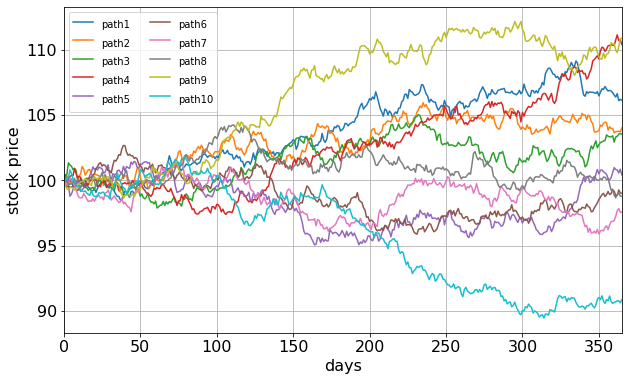
\includegraphics[width=0.7\textwidth]{figures/asset_price_simulation}
\caption{Simulation with Monte Carlo method of various realization of a stock price, using geometric Brownian motion.}
\label{fig:stock_price_sim}
\end{figure}

\subsection{Pricing Vanilla European Options by Monte Carlo}
Monte Carlo simulation fits particularly well to the pricing of a derivative: we can simulate different stock paths, calculate the average of the corresponding payoffs (i.e. the expectation), and finally discount the result.

Let's consider a vanilla European call option. This may seem a little pointless, as there is the Black-Scholes formula which provides an analytical method that easily delivers the true option price, nevertheless, it is a good example of financial simulation. 

The price $C$ of a call option with strike $K$ and duration $T$ is defined by

\begin{equation} 
C = e^{-rT} \mathbb{E}[(S(T)-K)^+ ]
\label{eq:call_payoff}
\end{equation}
However, it is impossible to price an option without any information about the distribution of its underlying price or its return. Therefore, we necessarily need to specify the particular distribution of the final asset price $S(T)$. 

Let's model $S(T)$ as a log-normal random variable and simulate one path for the asset price as shown before. Then calculate, according to Eq.~\ref{eq:call_payoff}, the corresponding payoff. Repeat this step numerous times and finally compute the mean of the discounted payoffs. 

The fact that this Monte Carlo estimate is indeed consistent with the Black-Scholes formula is illustrated in Fig.~\ref{fig:error_BS} where the distribution of 10000 simulations is plotted with the 95\% confidence interval. This is another indication that Monte Carlo provides correct results in the limit $n\rightarrow\infty$.

\begin{figure}[htb]
\centering
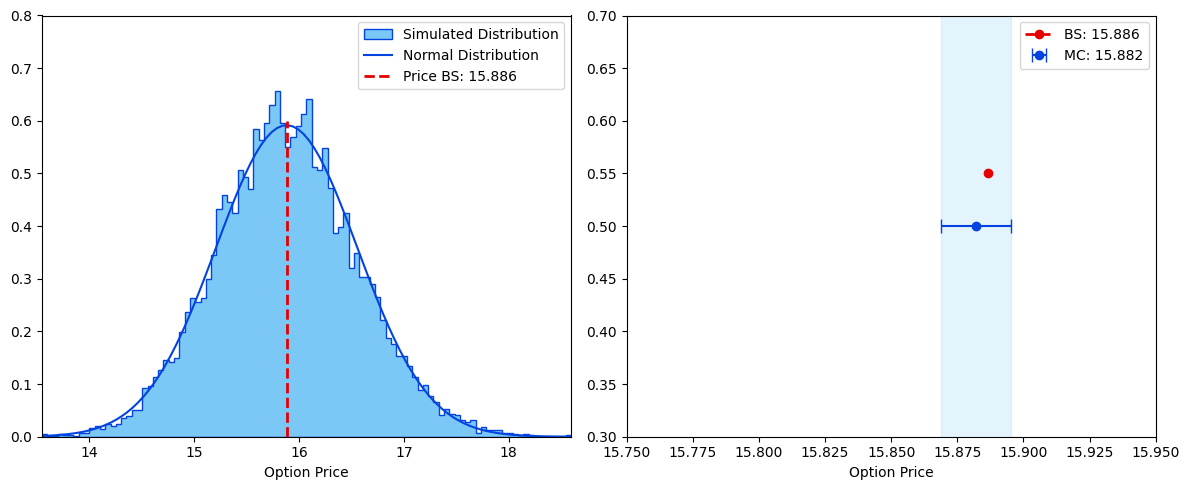
\includegraphics[width=0.9\textwidth]{figures/call_pricing_error.png}
\caption{Call option price: on the left the distribution of the results of 10000 MC simulation, on the right the 95\% confidence interval and the Black-Scholl price.}
\label{fig:error_BS}
\end{figure}

\section{Markov Chain}
\label{sec:markov_chain}
A \emph{Markov chain} is a mathematical system usually defined as a collection of random variables, that transition from one state to another according to certain probabilistic rules. This set of transitions satisfies the Markov property, in other words the probability of transitioning to any particular state is dependent solely on the current state and not on the sequence of states that preceded it. 

Markov Chains are widely employed in economics, game theory, communication theory, genetics and finance. When it comes to real-world problems, they are used to study cruise control systems in motor vehicles, queues or lines of customers, exchange rates of currencies\ldots

%A Markov chain is then a random process and has either discrete state space (set of possible values of the random variables) and discrete index set (often representing time). 

\subsection{Discrete Time Markov Chain}
A discrete-time Markov chain involves a system which is in a certain state at each step, with the state changing randomly. The steps are often thought of as moments in time (but you might as well refer to physical distance or any other discrete measurement). This kind of Markov chain is a sequence of random variables $X_1, X_2, X_3,\ldots$ with the Markov property. Putting this is mathematical probabilistic formula:

\begin{equation}
P(X_{n+1}) = x | X_1 = x_1, X_2 = x_2, \ldots, X_n = x_n) = P( X_{n+1} = x | X_n = x_n)
\end{equation}

The probability of $X_{n+1}$ only depends on the probability of $X_n$ that precedes it. Which means the knowledge of the previous state is all that is necessary to determine the probability distribution of the current state.

\begin{attention}
Some interesting properties of Markov chains are:

\begin{itemize}
\tightlist
\item reducibility: a Markov chain is said to be irreducible if there exists a chain of steps between any two states that has positive probability;
\item periodicity: a state in a Markov chain is periodic if the chain can return to the state only at multiples of some integer larger than 1. Otherwise the state is called aperiodic;	
\item transience and recurrence: a state $i$ is said to be transient if, given that we start in state $i$, there is a non-zero probability that we will never return to $i$. State $i$ is recurrent (or persistent) if it is not transient;
\item ergodicity: a state $i$ is said to be ergodic if it is aperiodic and recurrent. If all states in an irreducible Markov chain are ergodic, then the chain is said to be ergodic;
\item absorbing state: a state $i$ is called absorbing if it is impossible to leave this state. If every state can reach an absorbing state, then the Markov chain is an absorbing Markov chain.
\end{itemize}
\end{attention}

%The possible values of $X_i$ form a countable set $S$ called the state space of the chain. The state space can be anything: letters, numbers, basketball scores or weather conditions. While the time parameter is usually discrete, the state space of a discrete time Markov chain does not have any widely agreed upon restrictions, and rather refers to a process on an arbitrary state space. However, many applications of Markov chains employ finite or countably infinite state spaces, because they have a more straightforward statistical analysis.

\subsection{The Markov Model}
A Markov chain can be represented by a set of probabilities associated with the various possible transitions (the changes of state of the system). These probabilities are usually represented as a matrix (i.e. the \emph{transition matrix}).
Each element of the matrix $P(X_{n+1} = x | X_n = x_n)$ can be read as the probability of going to state $X_{n+1}$ given the current value of state $X_n$. 

If the Markov chain has $N$ possible states, the matrix will be $N \times N$, such that entry $(i, j)$ is the probability of transitioning from state $i$ to state $j$. Additionally, the transition matrix must be such that entries in each row must add up to exactly 1, since each row represents a state probability distribution.

%The model is characterized by a state space (the set of possible state of the system), a transition matrix describing the probabilities of particular transitions, and an initial state across the state space. Let's work out a real example. 

\subsection{Markov Chain to Predict Market Trends}
Markov chains and their respective diagrams can be used to model the probabilities of certain financial market climates and thus predicting the likelihood of future market conditions.
These conditions, also known as trends, are:
\begin{itemize}
\item bull markets: periods of time where prices generally are rising, due to the actors having optimistic hopes of the future;
\item bear markets: periods of time where prices generally are declining, due to the actors having a pessimistic view of the future;
\item stagnant markets: periods of time where the market is characterized by neither a decline nor rise in general prices.
\end{itemize}

The transition matrix is usually determined using historical data. For example, consider a hypothetical market with Markov properties where historical data has given us the patterns depicted in Fig.~\ref{fig:markov_chain}.
After a week characterized of a \emph{bull market} trend there is a 90\% chance that another bullish week will follow. Additionally, there is a 7.5\% chance that the bull week instead will be followed by a bearish one, or a 2.5\% chance that it will be a stagnant one. Similarly for the other states. 

\begin{figure}[htb]
\centering
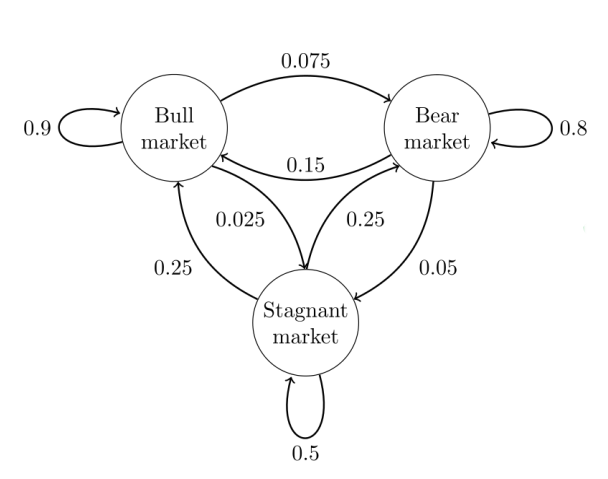
\includegraphics[width=0.7\textwidth]{figures/markov_chain}
\caption{Graph showing the transition probabilities between three weekly market states: bull, bear and stagnant.}
\label{fig:markov_chain}
\end{figure}

By compiling these probabilities into a table, it is easy to derive the transition matrix $\Pi$

\[\Pi = 
\begin{bmatrix}
p_{11} & p_{12} & p_{13} \\
p_{12} & p_{22} & p_{23} \\
p_{13} & p_{32} & p_{33}
\end{bmatrix} =
\begin{bmatrix}
0.9 & 0.075 & 0.025 \\
0.15 & 0.8 & 0.05 \\
0.25 & 0.25 & 0.5
\end{bmatrix} 
\]

Let's indicate with a $1 \times 3$ vector $C$ the current state of the market; where column 1 represents a bull week, column 2 a bear week and column 3 a stagnant week. Finally suppose this week the market is in a bearish state, resulting in the vector $C_0  = (0, 1, 0)$.

To calculate the probabilities of a bull, bear or stagnant week for any number of $n$ weeks into the future it is enough to multiply $C$ by the transition matrix $n$ times ($C_n = C_0\cdot \Pi^n$)

\[C_1 = C_0 \cdot \Pi =  
\begin{bmatrix}
0 \\
1 \\
0 
\end{bmatrix}
\begin{bmatrix}
0.9 & 0.075 & 0.025 \\
0.15 & 0.8 & 0.05 \\
0.25 & 0.25 & 0.5
\end{bmatrix} = 
\begin{bmatrix}
0.15 \\
0.8 \\
0.05 
\end{bmatrix}
\]

The model predicts an 80\% probability for the market to stay in a bearish mode also in the next week, 15\% to become bullish and just a 5\% to be stagnant.

With \texttt{python} it is possible to determine longer term behavior up to the \emph{stationary distribution}. The stationary distribution is the fraction of time that the system spends in each state as the number of iterations approaches infinity.

\begin{ipythonnon}
import numpy as np

n = 50
hist_C = np.zeros(shape=(n, 3))
C = np.array([0, 1, 0])
P = np.array([[0.9, 0.075, 0.025],[0.15, 0.8, 0.05],[0.25, 0.25, 0.5]])

for i in range(n):
    hist_C[i] = C
    C = C.dot(P)

print (C)
\end{ipythonnon}
\begin{ioutput}
[0.62499979 0.31250019 0.06250002]
\end{ioutput}

From this example it can be concluded that as $n \rightarrow \infty$, the probabilities will converge to a steady state, 63\% of all weeks will be bullish, 31\% bearish and 6\% stagnant. Figure~\ref{fig:markov_chain_sim} reports the various probabilities at each iteration. The system converges to the stationary state after about 20 weeks.
It can also be shown, by changing $C_0$ that the steady-state probabilities of this Markov chain do not depend upon the initial state. 

\begin{figure}[!t]
	\centering
	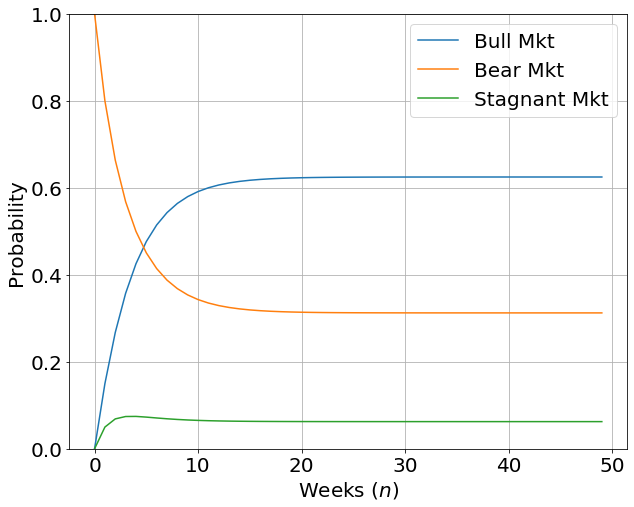
\includegraphics[width=0.7\textwidth]{figures/markov_chain_sim}
	\caption{Simulation of weekly market trend for $n=50$. The system reaches the stationary state relatively quickly after about 20 weeks.}
	\label{fig:markov_chain_sim}
\end{figure}

These results can be used in various ways, some examples are: calculating the average time it takes for a bearish period to end or the risk that a bullish market turns bearish or stagnant.

\subsection{The Generator Matrix}

As we have seen we can "evolve" a transition matrix by multiplying it by itself multiple times. Each multiplication move forward by a multiple of the original time horizon, e.g. in credit risk, a transition matrix $(P)$ shows the probability of a borrower’s credit rating changing from one grade to another over a specific period—typically one year, so $P^4$ represents the same probability for a 4 years horizon.
 
However, it is sometimes needed the probabilities for different time frames (e.g., a 3-month outlook). Converting a 1-year matrix to these "other horizons" involves specific mathematical approaches.
The most robust and "preferred" method for converting transition matrices to any arbitrary time horizon is using the \emph{Generator Matrix} $(A)$, often referred to as the \emph{Matrix Logarithm} approach.

In this case instead of just multiplying the matrix by itself, we treat the credit migration as a \emph{continuous-time Markov chain}. So first calculate the Generator Matrix $A$ from the observed $t$-year matrix $P$ as:
\begin{equation}
A = \frac{1}{t}\ln(P)
\end{equation}
Then scale that generator by the desired time horizon $(h)$ and finally convert it back to a probability matrix $(P_h)$ using the matrix exponential:
\begin{equation}
P_h = \exp(A\cdot h)
\end{equation}

This technique allows you to calculate transitions for non-integer periods (e.g., 0.5 years or 2.3 years) and ensures that the transition behavior remains mathematically consistent across all time slices.

The mathematical intuition behind the Generator Matrix relies on the transition from discrete jumps to continuous flow. The easiest way to visualize this is through interest rates.
If you have an annual interest rate, you multiply your principal by $(1+r)$ once a year. If interest is compounded every microsecond, you use the exponential function $e^{rt}$.

In credit risk, a standard transition matrix is discrete, i.e. a snapshot of what happened over 12 months. This method treats credit migration as a continuous process where a company's credit quality is "decaying" or "improving" every single second.

To move between horizons, we use the relationship between a probability matrix $(P)$ and a generator matrix $(A)$:
\begin{equation}
P(t)=\exp(At)=\sum_{k=0}^{\infty}\frac{(At)^k}{k!}
\end{equation}

This represents the "instantaneous intensity" of migration. The diagonal elements are negative (representing the rate at which a firm leaves its current rating), and the off-diagonal elements are positive (the rate at which it moves to others). The Matrix Exponential isn't just taking the $e$ of every number in the grid; it’s a power series expansion that accounts for all possible "paths" a borrower could take e.g., migrating from A to BBB and back to A within the time frame.

To find the generator $A$ from an observed 1-year matrix $P$, we perform a matrix logarithm, and once you have $A$, the time variable $t$ becomes a simple scaler, e.g. for a 6-month horizon $P_{0.5} = \exp(A\cdot 0.5)$.

For the math to work (for the logarithm to exist and result in real numbers), the matrix $P$ must be diagonally dominant. This means the probability of staying in the same rating must be significantly higher than the probability of moving. If a rating system is so volatile that more people leave a grade than stay in it, the "Preferred Method" fails because the matrix logarithm may result in complex numbers—essentially saying the "path" of credit risk is mathematically undefined.

\section*{Exercises}
\begin{question}
Using the Euler scheme, write a program to simulate:
\begin{itemize}
\tightlist
\item a Wiener process;
\item a Brownian motion with $S_0 = 100$, $\mu=0.05$ and $\sigma=0.17$;
\item the stock price following a Geometric Brownian motion with $S_0 = 100$, $\mu=0.05$ and $\sigma=0.17$.
\end{itemize}
\end{question}

\cprotEnv\begin{solution}
\begin{ipython}
from numpy.random import normal, seed
import numpy as np

S = 100
mu = 0.05
sigma = 0.17
T = 1
steps = 360

seed(1)
wiener = [S]
abm = [S]
gbm = [S]

for i in range(steps):
    wiener.append(wiener[-1] + normal()*np.sqrt(T/steps))
    abm.append(abm[-1] + mu * T/steps + sigma * np.sqrt(T/steps) * normal())
    S = S * np.exp((mu - 0.5 * sigma * sigma) * T/steps + sigma * \
                    np.sqrt(T/steps) * normal())
    gbm.append(S)
\end{ipython}

\begin{figure}[htbp]
\centering
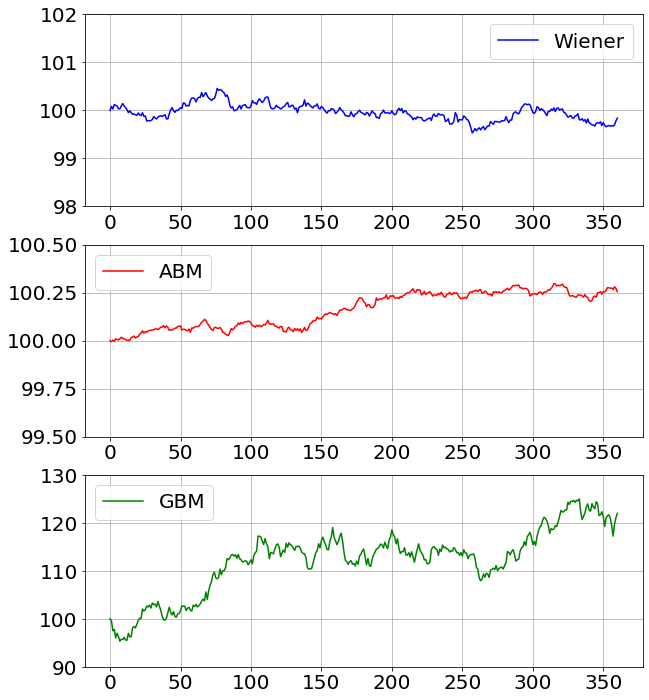
\includegraphics[width=0.5\linewidth]{figures/ex_stochastic}
\caption{Realizations of different kind of stochastic processes.}
\end{figure}
\end{solution}

\cprotEnv\begin{question}
Using the Euler scheme and a Monte Carlo simulation price an European vanilla call option

\begin{ipython}
S0 = 110
r = 0.05
sigma = 0.17
ttm = 1
K = 105
\end{ipython}

Plot the relative pricing difference (simulated price minus Black-Scholes price) versus the number of simulated scenarios (e.g. 10000 simulations).
Also measure the timing for the entire simulation and try to improve it.
\end{question}

\cprotEnv\begin{solution}
The reference price is the one computed using the Black-Scholes formula
\begin{ipython}
from finmarkets import call

S0 = 110
r = 0.05
sigma = 0.17
T = "1y"
K = 105

C0 = call(S0, K, r, sigma, T)

print ("BS call price: {:.2f}".format(C0))
\end{ipython}
\begin{ioutput}
BS call price: 13.28
\end{ioutput}

The first Monte Carlo implementation uses standard lists and for-loops
\begin{ipython}
import time
from math import exp, sqrt
from numpy.random import normal, seed

t1 = time.time()
S0 = 110
r = 0.05
sigma = 0.17
T = 1
K = 105

values = []
for sim in range(1, 10000):
  seed(sim)
  payoff = []
  for i in range(sim):
    St = S0 * exp((r - 0.5 * sigma * sigma) * T + sigma * sqrt(T) * normal())
    payoff.append(exp(-r*T)*max(0, St-K))
  values.append(sum(payoff)/sim)

Cs = []
for i in range(1, len(values)):
  Cs.append((sum(values[:i])/i - C0)/C0)

print ("Elapsed time: ", time.time() - t1)
\end{ipython}
\begin{ioutput}
Elapsed time:  296.0764889717102
\end{ioutput}

Plotting the relative difference between the MC and BS price it is apparent how the agreement improves as the number of simulations increases.

\begin{figure}[htbp]
\centering
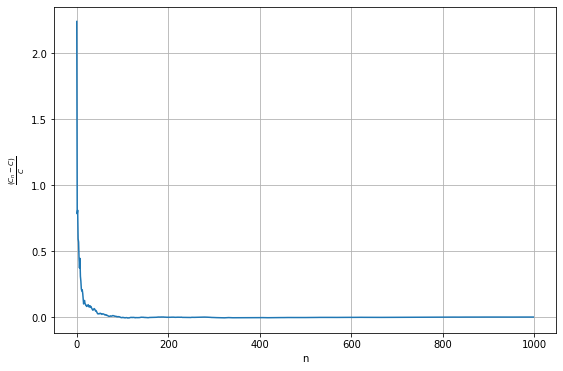
\includegraphics[width=0.7\linewidth]{figures/ex_call_pricing_error}
\caption{Call pricing difference as a function of the number of simulated scenarios.}
\end{figure}

The very same algorithm implemented using \texttt{numpy.array} is more concise, and more importantly, much faster since it runs in one hundredth of the time. Note that this is kind of cheating since we are relying on the \texttt{C} implementation underlying \texttt{numpy}.

\begin{ipython}
import numpy as np
import time
from scipy.stats import norm

t1 = time.time()
S0 = 110
r = 0.05
sigma = 0.17
T = 1
K = 105

Cs = []
for i in range(1, 10000):
  np.random.seed(i)
  Z = norm.rvs(size=i)
  St = S0 * np.exp((r - 0.5 * sigma ** 2) * T + sigma * np.sqrt(Tt) * Z)
  Cs.append(np.mean(np.exp(-r * T) * np.maximum(St - K, 0)))

n = 1/np.arange(1, 10000)
c = np.cumsum(Cs)*n

print ("Elapsed time: ", time.time() - t1)
\end{ipython}
\begin{ioutput}
Elapsed time:  4.282579183578491
\end{ioutput}
\end{solution}

\begin{question}
Assume that a man’s profession can be classified as professional, skilled labourer, or unskilled labourer. Assume that, of the sons of professional men, 80 percent are professional, 10 percent are skilled labourers, and 10 percent are unskilled labourers.

In the case of sons of skilled labourers, 60 percent are skilled labourers, 20 percent are professional, and 20 percent are unskilled. Finally, in the case of unskilled labourers, 50 percent of the sons are unskilled labourers, and 25 percent each are in the other two categories. Assume that every man has at least one son, and form a Markov chain by following the profession of a randomly chosen son of a given family through several generations. Set up the matrix of transition probabilities. Find the probability that a randomly chosen grandson of an unskilled labourer is a professional man.
\end{question}

\cprotEnv\begin{solution}
The Markov chain in this exercise has the following set states
\begin{equation*}
S = \{\textrm{Professional, Skilled, Unskilled}\}
\end{equation*}
with the following transition probabilities:

\begin{table}[htbp]
\centering
\begin{tabular}{l c c c}
&Professional& Skilled &Unskilled \\
Professional & .8 & .1 & .1 \\
Skilled & .2 & .6 & .2 \\
Unskilled & .25 & .25 & .5 \\
\end{tabular}
\end{table}
\noindent
so that the transition matrix for this chain is

\begin{equation*}
\Pi =
\begin{bmatrix}
.8 &.1 &.1\\
.2 &.6 &.2\\
.25 &.25 &.5
\end{bmatrix}
\end{equation*}

Since we are interested to find the probability that a grandson of an unskilled labourer is a professional we need to apply twice the transition matrix to the initial state $C=(0, 0, 1)$.
\begin{ipython}
import numpy as np

C = np.array([0,0,1])
P = np.array([[.8, .1,.1],[.2,.6,.2],[.25,.25,.5]])

C_grandson = C.dot(P).dot(P)
print (C_grandson[0])
\end{ipython}
\begin{ioutput}
0.375
\end{ioutput}
\end{solution}

\begin{question}
Consider an experiment of mating rabbits. We watch the evolution of a particular gene that appears in two types, $G$ or $g$. A rabbit has a pair of genes, either $GG$ (dominant), $Gg$ (hybrid, the order is irrelevant, so $gG$ is the same as $Gg$) or gg (recessive).

In mating two rabbits, the offspring inherits a gene from each of its parents with equal probability. Thus, if we mate a dominant ($GG$) with a hybrid ($Gg$), the offspring is dominant with probability 1/2 or hybrid with probability 1/2.
Start with a rabbit of given character ($GG$, $Gg$, or $gg$) and mate it with a hybrid. The offspring produced is again mated with a hybrid, and the process is repeated through a number of generations, always mating with a hybrid.
\begin{tasks}
\task Write down the transition probabilities of the Markov chain thus defined;
\task assume that we start with a hybrid rabbit. Let $\mu_n$ be the probability distribution of the character of the rabbit of the n$^{th}$ generation. In other words, $\mu_n(GG)$, $\mu_n(Gg)$, $\mu_n(gg)$ are the probabilities that the n$^{th}$ generation rabbit is $GG$, $Gg$, or $gg$, respectively. Compute $\mu_1$, $\mu_2$, $\mu_3$.
\end{tasks}
\end{question}

\cprotEnv\begin{solution}
The set of states is 
\begin{equation*}
S = \{\textrm{GG, Gg, gg}\}
\end{equation*}
with the following transition probabilities:

\begin{table}[htbp]
\centering
\begin{tabular}{l c c c}
&GG& Gg & gg \\
GG & .5 & .5 & 0 \\
Gg & .25 & .5 & .25 \\
gg & 0 & .5 & .5 \\
\end{tabular}
\end{table}
\noindent
We can rewrite the transition matrix in the following form:

\begin{equation*}
\Pi =
\begin{bmatrix}
.5 &.5 &0\\
.25 &.5 &.25\\
0 &.5 &.5
\end{bmatrix}
\end{equation*}

The elements from the second row of the matrix $\Pi^n$ will give us the probabilities for a hybrid to give dominant, hybrid or recessive species in $(n − 1)^{th}$ generation in this experiment, respectively (reading this row from left to right).
\begin{ipython}
import numpy as np

P = np.array([[.5,.5,0],[.25,.5,.25],[0,.5,.5]])

mu1 = P[1, :]
mu2 = P.dot(P)[1, :]
mu3 = P.dot(P).dot(P)[1, :]

print (mu1)
print (mu2)
print (mu3)
\end{ipython}
\begin{ioutput}
[0.25 0.5  0.25]
[0.25 0.5  0.25]
[0.25 0.5  0.25]
\end{ioutput}
so that $\mu_i(GG) = .25, \mu_i(Gg) = .5, \mu_i(gg) = .25$, $i = 1, 2, 3$.
Actually the probabilities are the same for any $i \in \mathbb{N}$. 

\begin{curiosity}
If you obtained this result before 1858 when Gregor Mendel started to breed garden peas in his monastery garden and analysed the offspring of these matings, you would probably be very famous because it definitely looks like a law! This is what Mendel found when he crossed mono-hybrids.
\end{curiosity}
\end{solution}











\chapter{Black-Scholes Model}
\label{ch:BS}

\section{Black-Scholes Model}
Suppose that stock price $S$ follows a geometric Brownian motion

\begin{equation}
dS = \mu Sdt + \sigma SdW
\label{eq:bs_gbm}
\end{equation}
we are going to derive a partial differential equation (PDE) for the price of a derivative based on such a stock.

The model proposed by Black and Scholes relies on the following set of additional assumptions (besides the geometric Brownian motion):
\begin{itemize}
\tightlist 
\item constant risk-less interest rate $r$;
\item no transaction costs;
\item it is possible to buy/sell any (also fractional) number of stocks; similarly with the cash;
\item no restrictions on short selling;
\item option is of European type.
\end{itemize}

After the derivation of the model equation we will determine the explicit solution for European call and put options.

\subsection{Merton Derivation}
In this Section we are going to provide the steps followed by Merton to derive the Black-Scholes PDE.

Firstly, let's consider the case of a non-dividend paying stock. Imagine a portfolio consisting of options, stocks and cash with the properties that at each time $t$ the portfolio has zero value and it is \emph{self-financing}, which means that if there is no exogenous infusion or withdrawal of money, the purchase of a new asset must be financed by the sale of an old one. Let be 
\begin{itemize}
\item $Q_S$, the number of stocks, each of them with value $S$;
\item $Q_V$, number of options, each of them with value $V$;
\item $B$, cash on the account, which is continuously compounded using the risk-free rate $r$.
\end{itemize}
The required properties can be formulated mathematically as
\begin{equation}
\begin{cases}
SQ_S+VQ_V+B=0 \\
SdQ_S + V dQ_V +\delta B = 0 \\
dB = rBdt+\delta B
\end{cases}
\label{eq:bs_properties}
\end{equation}
Differentiating the first of Eq.~\ref{eq:bs_properties}
\begin{equation}
\begin{split}
&d(SQ_S + VQ_V +B) = d(SQ_S + VQ_V) + \overbrace{dB}^{rBdt+\delta B} = 0 \\
& \overbrace{SdQ_s + VdQ_V +\delta B}^{=0} + Q_S dS + Q_V dV + rBdt = 0 \\
& Q_SdS+Q_VdV \overbrace{-r(SQ_S + VQ_V)}^{rB}dt=0\\
\end{split} 
\end{equation}
Dividing by $Q_V$ and setting $\Delta = -\frac{Q_S}{Q_V}$
\begin{equation}
dV -rVdt-\Delta (dS - rSdt)=0
\end{equation}
$dS$ can be determined from Eq.~\ref{eq:bs_gbm}, while $dV$ applying It$\hat{o}$'s lemma. Then we choose $\Delta$ (i.e. the ratio between the number of stocks and options) so that it eliminates the randomness (i.e. the coefficient at $dW$ is zero).
  
\begin{equation}
dV = \left(\cfrac{\partial V}{\partial t} + \mu S  \cfrac{\partial V}{\partial S} + \cfrac{1}{2} \sigma^2 S^2  \cfrac{\partial^2 V}{\partial S^2} \right) dt + \sigma S \cfrac{\partial V}{\partial S} dW
\end{equation} 
Therefore:
\begin{equation}
dP =  \left(\cfrac{\partial V}{\partial t} + \mu S  \cfrac{\partial V}{\partial S} + \cfrac{1}{2} \sigma^2 S^2  \cfrac{\partial^2 V}{\partial S^2} + \delta \mu S\right) dt + \left(\sigma S  \cfrac{\partial V}{\partial S} + \delta \sigma S \right)dW
\end{equation}
We eliminate the randomness
\begin{equation}
\delta = -\cfrac{\partial V}{\partial S}
\end{equation}

\begin{equation}
\cfrac{\partial V}{\partial t} + \cfrac{1}{2} \sigma^2 S^2 \cfrac{\partial^2 V}{\partial S^2}+ rS \cfrac{\partial V}{\partial S} - rV = 0
\end{equation}

\section{Solutions of Black-Scholes PDE}
Now we need to find a solution $V(S, t)$ to the partial differential equation which holds for $S >0$, $t \in [0, T)$.

So far we have not used the fact that we consider an option (in general the PDE holds for any derivative that pays a payoff at time $T$ depending on the stock price at this time).
Clearly the type of derivative determines the terminal condition at time $T$, so in general $V(S, T)$ = payoff of the derivative.

\subsection{Simple Solutions}
How to price the derivatives with the following payoffs:
\begin{itemize}
\tightlist
\item $V(S, T) = S$, it is in fact a stock so $V(S, t) = S$
\item $V(S, T) = E$ with a certainty we obtain the cash $E$ ($V(S, t) = Ee^{-r(T-t)}$)
\end{itemize}
by substitution into the PDE it is possible to check that they are indeed solutions.
%EXERCISES:
%Find the price of a derivative with payoff
%$V(S, T) =S^n$,where $n\in N$.

%HINT: Look for the solution in the form
%$V(S, t) =A(t)S^n$

%Find all solutions to the Black-Scholes PDE, which are independent of time, i.e., for which
%$V(S, t) = V(S)$

\subsection{Binary Options}
Let us consider a binary option, which pays \$1 if the stock price is higher than $K$ at expiration time, otherwise its payoff is zero.
In this case
\begin{equation}
V(S, T) = 
\begin{cases}
  1, \quad\textrm{if }S > K\\
  0, \quad\textrm{otherwise}	
\end{cases}
\end{equation}

This partial differential equation (PDE) can be solved directly with numerical methods. But then some tricky stability issues must be tackled. Here we prefer applying variable transformations as much as possible in order to obtain a simpler form (i.e. the goal is to re-formulate Black-Scholes PDE into a heat equation).

The first step is to apply the transformation $x = \textrm{ln}(S/K)$ and a new function $Z(x, \tau) = V (Ee^x, T -\tau)$. 
The PDE for $Z(x, \tau)$ becomes:
\begin{equation}
\begin{gathered}
\cfrac{\partial Z}{\partial \tau}-\cfrac{1}{2}\sigma^2 \cfrac{\partial^2 Z}{\partial x^2}+\left(\cfrac{\sigma^2}{2}-r\right)  \cfrac{\partial Z}{\partial x} + rZ = 0\\ \\
Z(x, 0) =V(Ee^x, T)
\end{gathered}
\end{equation}
Then consider the new function $u(x,\tau)=e^{\alpha x + \beta\tau}Z(x,\tau)$ where the constants $\alpha, \beta \in \mathbb{R}$ are chosen so that the PDE for $u$ is the heat equation.

The corresponding PDE for $u$ is
\begin{equation}
\begin{gathered}
\cfrac{\partial u}{\partial \tau} -\cfrac{\sigma^2}{2} \cfrac{\partial^2 u}{\partial x^2}+A\cfrac{\partial u}{\partial x} + Bu = 0\\ \\
u(x,0)=e^{\alpha x}Z(x,0)=e^{\alpha x}V(Ke^x, T)
\end{gathered}
\end{equation}
where
\begin{equation}
\begin{cases}
A=\alpha\sigma^2 + \cfrac{\sigma^2}{2}-r\\
B=(1+\alpha)r-\beta-\cfrac{\alpha^2\sigma^2+\alpha\sigma^2}{2}
\end{cases}
\end{equation}
In order to have $A=B=0$ to get the heat equation we set
\begin{equation}
\begin{cases}
\alpha=\cfrac{r}{\sigma^2}-\cfrac{1}{2}\\
\beta=\cfrac{r}{2}+\cfrac{\sigma^2}{8}+\cfrac{r^2}{2\sigma^2}
\end{cases}
\end{equation}
The solution $u(x,\tau)$ of the resulting PDE is given by the \emph{Green formula}
\begin{equation}
u(x, \tau)=\cfrac{1}{\sqrt{2\sigma^2\pi\tau}}\int^{+\infty}_{-\infty}e^{-\frac{(x-s)^2}{2\sigma^2\tau}}u(s,0)ds
\end{equation}

After evaluating the integral it is possible to find the original solution $V(S,t)$ performing backward substitutions

\begin{equation}
V(S, t) = e^{-r(T-t)}N(d_2)
\end{equation}
where $d_2=\frac{\textrm{log}(\frac{S}{K}+\left(r-\frac{\sigma^2}{2}\right)(T-t)}{\sigma\sqrt{T-t}}$.

\subsection{Call Options}
In this case
\begin{equation}
V(S,T)=\textrm{max}(0,S-K)=
\begin{cases}
S-K,\quad \textrm{if}~S>K\\
0, \quad\textrm{otherwise}
\end{cases}
\end{equation}

The steps are similar to the previous example (i.e. same sequence of transformations, initial conditions for the heat equation):
\begin{equation}
u(x,0)=
\begin{cases}
e^{\alpha x}(S-K),\quad \textrm{if}~x>0\\
0, \quad\textrm{otherwise}
\end{cases}
\end{equation}
and similar evaluation of the integral. Finally the option price
\begin{equation}
V(S,t) = SN(d_1)-Ke^{-r(T-t)}N(d_2)
\end{equation}
where $N$ is the distribution function of a normalized normal distribution and  $d_1=\frac{\textrm{log}(\frac{S}{K}+\left(r+\frac{\sigma^2}{2}\right)(T-t)}{\sigma\sqrt{T-t}}$, $d_2=d_1-\sigma\sqrt{T-t}$.

Figure~\ref{fig:call_option} shows the option price as a function of the stock price for various values of $t$.

\begin{figure}[htb]
  \centering
  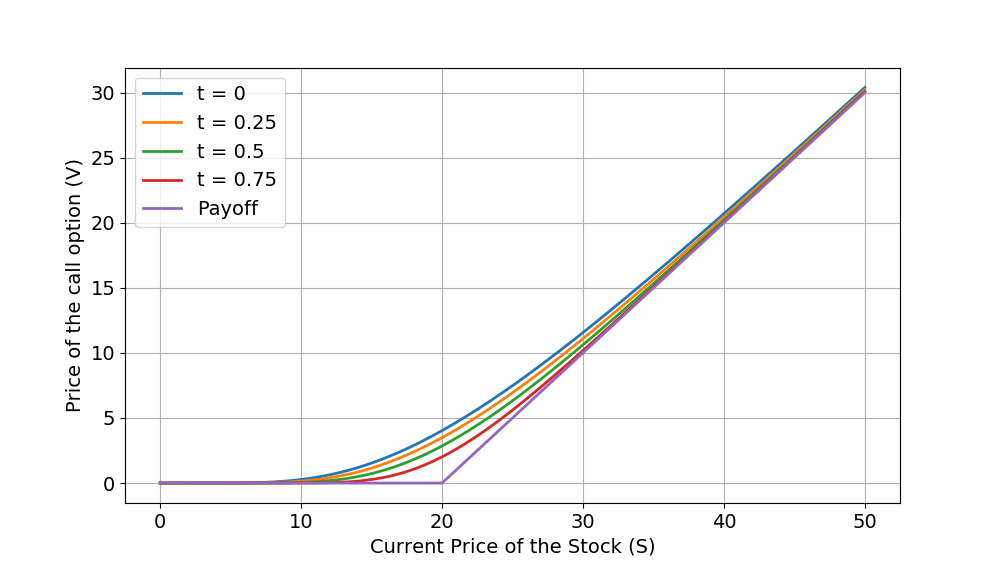
\includegraphics[width=0.9\textwidth]{figures/call_option_price}
  \caption{Option price as a function of the underlying price for various values of $t$.}
  \label{fig:call_option}
\end{figure}

\section{Asian Options}
\label{sec:asian_option}

An Asian option is a special option where the payoff is determined by \emph{the average underlying price over some preset-set period of time}; 
Asian options are thus one of the basic forms of exotic options. 

One advantage of Asian options is that these reduce the risk of market manipulation of the underlying instrument at maturity.
Because of the averaging feature, Asian options reduce the volatility inherent in the option; therefore, Asian options are typically cheaper than European or American options. 

There are numerous permutations of Asian option; the most basic are listed below:
\begin{itemize}
\item \textbf{Fixed strike} Asian call payout
$C(T)={\text{max}}\left(A(0,T)-K,0\right),$
where $A$ denotes the average price for the period $[0, T]$, and $K$ is the strike price. 
The equivalent put option is given by
$P(T)={\text{max}}\left(K-A(0,T),0\right)$.

\item The \textbf{floating strike} Asian call option has the payout
$C(T)={\text{max}}\left(S(T)-kA(0,T),0\right),$
where $S(T)$ is the price at maturity and $k$ is a weighting, usually 1 so often omitted from descriptions.
The equivalent put option payoff is given by
$P(T)={\text{max}}\left(kA(0,T)-S(T),0\right)$.
\end{itemize}

The average $A$ may be obtained in many ways. Conventionally, this means an arithmetic average. In the continuous case, this is obtained by
$A(0,T)={\frac  {1}{T}}\int _{{0}}^{{T}}S(t)dt$.
For the case of discrete monitoring (with monitoring at the times 
$0=t_{0},t_{1},t_{2},\dots ,t_{n}=T$ we have the average given by
$A(0,T)=\frac{1}{n}\sum_{i=1}^{n}S(t_{i})$.

There also exist Asian options with geometric average; in the continuous case, this is given by
$A(0,T)=\exp \left(\frac{1}{T}\int_0^T \log(S(t))dt\right)$.

\subsection{Pricing of Asian options}
We are able to derive a closed-form solution only for the geometric Asian option.
This is given by 
\begin{equation}
\begin{aligned}
C_A&=S_{0}e^{(b-r)T}\Phi (d_{1})-Ke^{-rT}\Phi (d_{2})\\
P_A&=Ke^{-rT}\Phi (-d_{2})-S_{0}e^{(b-r)T}\Phi (-d_{1})
\end{aligned}
\end{equation}
where 
\begin{equation}
\begin{aligned}
b&=\frac{1}{2}\left(r-\frac{1}{2}\sigma _A^2\right)\\
\sigma _A&=\frac{\sigma}{\sqrt{3}} \\
d_1 &=\log{\frac{S_0}{K}}+\left(b+\frac{1}{2}\sigma^2_A\right)\frac{T}{\sigma_A \sqrt{T}},\quad d_2=d_1-\sigma_A \sqrt {T}
\end{aligned}
\end{equation}

The arithmetic average type instead needs to be estimated with Monte Carlo techniques.


\section{Longstaff-Schwartz algorithm}
The Longstaff-Schwartz algorithm, widely known as the \emph{Least Squares Monte Carlo} (LSM) approach, represents a seminal advancement in financial engineering for valuing derivatives with early-exercise features.
Unlike European options, which only require a forward-looking simulation to maturity, American options present an optimal stopping problem where the holder must decide at every moment whether the immediate 
"intrinsic value" exceeds the expected value of all future payoffs, known as the \emph{continuation value}. Because this expectation is conditional on the state of the market at time $t$, it cannot be solved through simple forward simulation alone.

The LSM approach elegantly sidesteps the "curse of dimensionality" that plagues traditional lattice-based methods (like binomial trees) by combining Monte Carlo simulation with \emph{cross-sectional regression}. 

The algorithm operates in two distinct phases. Initially, it performs a forward pass to generate a large number of stochastic paths for the underlying asset(s) using Geometric Brownian Motion or other jump-diffusion models. Once the paths are secured, it executes a backward induction process starting from the final expiration date and moving toward the present.

At each discrete time step, the algorithm isolates the paths that are currently "in-the-money." It then uses the realized \emph{future cash flows} from those paths as the dependent variable in a least-squares regression, where the independent variables are the \emph{current asset prices} transformed by a set of basis functions (such as Laguerre, Hermite, or simple power polynomials).

This regression provides a functional approximation of the continuation value. By comparing this estimate against the immediate exercise payoff, the algorithm establishes an optimal exercise rule for each path. 
If the immediate payoff is higher, the path is "exercised," and the future cash flow for that path is updated to the current payoff; otherwise, the future cash flow is simply discounted back one step. 
By the time the induction reaches $t=0$, the average of these optimized, discounted cash flows provides the Net Present Value (NPV) of the American option. This methodology is particularly robust for multi-asset options and complex path-dependent structures where traditional partial differential equation (PDE) solvers become computationally prohibitive.

As an example consider the evaluation of an American put option using the Longstaff-Schwartz algorithm. The initial underlying value is $S_0=36$, the volatility is 20\%, the strike price $K=40$, $T=1$, and the risk-free rate 6\% flat.

We start with the forward pass represented by the simulation of $N$ paths of the stock price until maturity T. Then, starting from the last exercise date we apply the stopping rule; at any time $t$ you have a choice:
either exercise (receive $K-S_t$ for a put) or continue (receive $\mathbb{E}[V(t+1) e^{-rt}|S_t]$).
Plotting the future  payoffs against the underlying price we can see that the analytical price for a put interpolated the cloud of Monte Carlo points, see Fig.~\ref{fig:longstaff_fit}(left). 
This suggest us that the price at time $t_1$ can be computed by means of an average on all discounted payoff (i.e. the barycentre of the cloud made of discounted payoff). 
Which in turn suggests that the future value of an option can be seen as the problem of finding the curve that best fits the cloud of discounted payoff up to the date of interest.
So we have an empirical pricing formula for the put to be used in the Monte Carlo Simulation
\begin{equation}
	P(t_1,T,S(t_1),K)=c_0+c_1 S(t_1) + c_2 S(t_1)^2 + c_3 S(t_1)^3 + c_4 S(t_1)^4 + c_5 S(t_1)^5
\end{equation}
Since we don't know the "true" expected value of continuing, we approximate it using the cross-section of all simulated paths. We regress the realized future payoffs against the current stock price.
If the regression says "exercising is better," we replace that path's future cash flow with the immediate payoff.

\begin{figure}[htb]
	\centering
	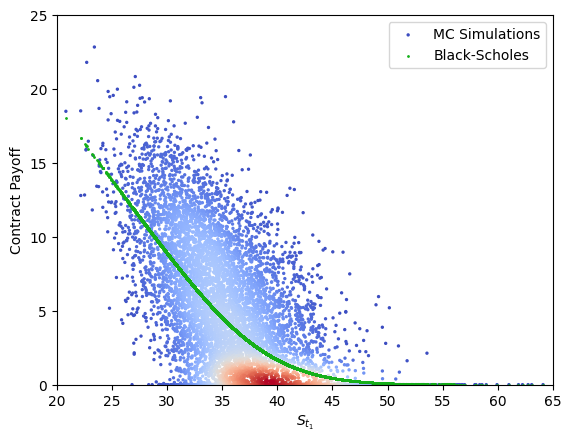
\includegraphics[width=0.45\textwidth]{figures/longstaff_fit}
	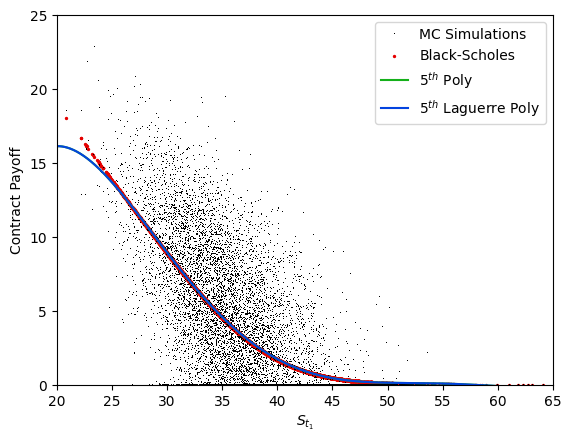
\includegraphics[width=0.45\textwidth]{figures/longstaff_fit_2}
	\caption{(Left) Scatter plot of the contract payoff and the underlying value ($S_t$) at time $t_1$. The green line represents the analytical price computed using Black-Scholes model. (Right) Cross-sectional
		regression of the contract payoff with two fifth order polynomials.}
	\label{fig:longstaff_fit}
\end{figure} 

\begin{ipythonnon}
import numpy as np
	
from datetime import date
	
from finmarkets.utils import OptionType 
from finmarkets import DiscountCurve, TimeInterval
	
def payoff(S0, K, T, r, sigma, n_paths, t_steps, option_type=OptionType.Call):    
  S = GBM(r, sigma, S0, T, t_steps, n_paths)    
	
  if option_type == OptionType.Put:
    payoffs = np.maximum(K - S, 0)
  else:
    payoffs = np.maximum(S - K, 0)
  return S, payoffs
	
def longstaff-schwarz(today, paths, payoffs, dc):    
  t_steps, n_paths = paths.shape
  dt = 1 / t_steps
	
  value = payoffs[-1]
	
  for t in range(t_steps - 1, 0, -1):
    itm_idx = np.where(payoffs[t] > 0)[0]
    df = dc.df(today+TimeInterval(f"{t}d"))
    if len(itm_idx) > 0:
      X = S[t, itm_idx]
      Y = value[itm_idx] * dc.df(today+TimeInterval(f"{t}d"))
      coeffs = np.polynomial.laguerre.lagfit(X, Y, 5)
      continuation_value = np.polynomial.laguerre.lagval(X, coeffs)	
      exer_now = payoffs[t, itm_idx]	
      exer_mask = exer_now > continuation_value
      value[itm_idx[exer_mask]] = exer_now[exer_mask]
	
      non_exer_mask = ~exer_mask
      value[itm_idx[non_exer_mask]] = value[itm_idx[non_exer_mask]] * df
	
      otm_idx = np.setdiff1d(np.arange(n_paths), itm_idx)
      value[otm_idx] = value[otm_idx] * df
    else:
      value = value * df
    return np.mean(value * dc.df(today+TimeInterval(f"{1}d")))
	
obs_date = date.today()
dates = [obs_date + TimeInterval(f"{i}m") for i in range(13)]
dc = DiscountCurve(dates, np.array([np.exp(-r*t/12) for t in range(13)]))
	
S, payoffs = payoff(36, 40, 1, 0.06, 0.2, 25000, 365, OptionType.Put)
	
npv = american_option_lsm(obs_date, S, payoffs, dc)
print(f"American Option NPV: {npv:.4f}")	
\end{ipythonnon}
\begin{ioutput}
	American Option NPV: 3.9954
\end{ioutput}


%\subsection{Asian Option Pricing with Monte Carlo}
%
%Every time a Monte Carlo simulation is run, we get an estimate of the quantity we are trying to calculate. It is desirable to quantify how precise our estimate is through the "standard error" (i.e. confidence interval).
%
%As we have seen above an obvious way to make our estimate more precise is to increase the number $N$ of simulations (e.g. random price paths) considered. However this can be computationally expensive therefore different methods have been developed, namely \emph{variance reduction techniques}.


%\subsubsection{Control Variate Variance Reduction Method}
%
%Say desired simulation quantity is $\mathbb{E}[X]$, and there is another known random variable $Y$ with known analytical expectation $\mu_Y = \mathbb{E}[Y]$. For any constant $c$ one can see that $Z = X + c\cdot(Y -\mu_Y)$ is an unbiased estimator of $X$, by linearity of expectation. Also it can be shown that $\var(Z) = \var(X) + 2c\cdot \var(Y) + 2c\cdot\cov(X; Y)$ is minimized when $c = -\frac{\cov(X;Y)^2}{\var(Y)}$. 
%$Y$ is called a \textbf{control variate} of $X$. 
%
%To reduce variance, $Y$ can be chosen as much correlated as possible with $X$. In practice, we can select a $Y$ which is approximately equal to $X$, easy to simulate and whose expectation is known. 
%
%In our case given that $X$ is the payoff of an Asian Option with Arithmetic average, these requirements are satisfied perfectly when we take $Y$ to be the Asian Option payoff with Geometric average (a closed form solution for its price is known).
%
%In practice we are going to simulate a set of paths for the underlying and compute $Z$ from  $X$, $Y$ and $\mu_Y$.
%
%\begin{finmarkets}
%The following class \texttt{AsianOption} implements all the methods described above besides the analytical pricing formula of the Geometric average Asian option.
%\end{finmarkets}
%
%\pythoncodenon{code/options_asian.py}
%
%\subsubsection{An Example}
%We are going to consider an Asian Option (fixed strike) with the following properties
%\begin{ipythonnon}
%S0 = 100 #underlying price
%K = 100 # strike
%tau = 1 # time to maturity (years)
%sigma = 0.2 # volatility
%r = 0.05 # constant risk-free rate
%\end{ipythonnon}
%and compare the results from the different Monte Carlo techniques.
%
%The baseline result is represented by a "naive" Monte Carlo simulation where various underlying price paths are generated with the Euler scheme. The option price is determined as the mean of the discounted payoffs corresponding to each simulation
%\begin{equation*}
%C = \frac{1}{N}\sum_{i=1}^{N} e^{-r\tau}\max(0, A_i(0, \tau)-K)
%\end{equation*}
%
%Baseline results are compared to analogous simulations performed with antithetic and control variate techniques.
%Figures~\ref{fig:asian_mc_results} shows the comparison of prices and uncertainties as a function of $N$ and $K=100$.
%In general the larger the number of simulations, the more accurate the estimate.
%One can see also that with control variates, the option value is almost constant, whereas the naive implementation tends to jump around before converging.
%
%%\begin{table}[htbp]
%%\begin{center}
%%\begin{tabular}{l|c|c|c|c|c} 
%%  \hline
%%  & 80 & 90 & 100 & 110 & 120 \\
%%  \hline
%%  100 & 20.845 & 12.005 & 5.250 & 1.549 & 0.386 \\ 
%%  \hline
%%  1000 & 21.403 & 12.455 & 5.670 & 1.949 & 0.531 \\ 
%%  \hline
%%  10000 & 21.313 & 12.434 & 5.621 & 1.915 &  0.496 \\ 
%%  \hline
%%  100000 & 21.461 & 12.553 & 5.721 & 1.967 &  0.519 \\ 
%%  \hline
%%  1000000 & 21.489 & 12.591 & 5.754 & 1.981 &  0.522 \\ 
%%\end{tabular}
%%\end{center}
%%\end{table}
%%
%%
%%\begin{table}[htbp]
%%\begin{center}
%%\begin{tabular}{l|c|c|c|c|c} 
%%  \hline
%%  & 80 & 90 & 100 & 110 & 120 \\
%%  \hline
%%  100 & 1.0870 & 0.9900 & 0.7425 & 0.4388 & 0.2595 \\ 
%%  \hline
%%  1000 & 0.3543 & 0.3292 & 0.2524 & 0.1560 & 0.0807 \\ 
%%  \hline
%%  10000 & 0.1118 & 0.1027 & 0.0783 & 0.0473 &  0.0231 \\ 
%%  \hline
%%  100000 & 0.0335 & 0.0328 & 0.0251 & 0.0153 &  0.0077 \\ 
%%  \hline
%%  1000000 & 0.0113 & 0.0104 & 0.0080 & 0.0049 &  0.0025 \\ 
%%\end{tabular}
%%\end{center}
%%\end{table}
%%
%%
%%\begin{table}[htbp]
%%\begin{center}
%%\begin{tabular}{l|c|c|c|c|c} 
%%  \hline
%%  & 80 & 90 & 100 & 110 & 120 \\
%%  \hline
%%  100 & 20.845 & 12.005 & 5.250 & 1.549 & 0.386 \\ 
%%  \hline
%%  1000 & 21.403 & 12.455 & 5.670 & 1.949 & 0.531 \\ 
%%  \hline
%%  10000 & 21.313 & 12.434 & 5.621 & 1.915 &  0.496 \\ 
%%  \hline
%%  100000 & 21.461 & 12.553 & 5.721 & 1.967 &  0.519 \\ 
%%  \hline
%%  1000000 & 21.489 & 12.591 & 5.754 & 1.981 &  0.522 \\ 
%%\end{tabular}
%%\end{center}
%%\end{table}
%%
%%
%%\begin{table}[htbp]
%%\begin{center}
%%\begin{tabular}{l|c|c|c|c|c} 
%%  \hline
%%  & 80 & 90 & 100 & 110 & 120 \\
%%  \hline
%%  100 & 1.0870 & 0.9900 & 0.7425 & 0.4388 & 0.2595 \\ 
%%  \hline
%%  1000 & 0.3543 & 0.3292 & 0.2524 & 0.1560 & 0.0807 \\ 
%%  \hline
%%  10000 & 0.1118 & 0.1027 & 0.0783 & 0.0473 &  0.0231 \\ 
%%  \hline
%%  100000 & 0.0335 & 0.0328 & 0.0251 & 0.0153 &  0.0077 \\ 
%%  \hline
%%  1000000 & 0.0113 & 0.0104 & 0.0080 & 0.0049 &  0.0025 \\ 
%%\end{tabular}
%%\end{center}
%%\end{table}
%%
%%\begin{table}[htbp]
%%\begin{center}
%%\begin{tabular}{l|c|c|c|c|c} 
%%  \hline
%%  & 80 & 90 & 100 & 110 & 120 \\
%%  \hline
%%  100 & 21.385 & 12.377 & 5.577 & 1.761 & 0.428 \\ 
%%  \hline
%%  1000 & 21.483 & 12.561 & 5.723 & 1.939 & 0.508 \\ 
%%  \hline
%%  10000 & 21.472 & 12.576 & 5.720 & 1.967 &  0.517 \\ 
%%  \hline
%%  100000 & 21.476 & 12.572 & 5.731 & 1.963 &  0.512 \\ 
%%  \hline
%%  1000000 & 21.483 & 12.585 & 5.749 & 1.979 &  0.521 \\ 
%%\end{tabular}
%%\end{center}
%%\end{table}
%%
%%\begin{table}[htbp]
%%\begin{center}
%%\begin{tabular}{l|c|c|c|c|c} 
%%  \hline
%%  & 80 & 90 & 100 & 110 & 120 \\
%%  \hline
%%  100 & 0.1299 & 0.3639 & 0.2373 & 0.2925 & 0.1592 \\ 
%%  \hline
%%  1000 & 0.0464 & 0.1233 & 0.0817 & 0.0999 & 0.0555 \\ 
%%  \hline
%%  10000 & 0.0135 & 0.0390 & 0.0253 & 0.0312 &  0.0166 \\ 
%%  \hline
%%  100000 & 0.0043 & 0.0123 & 0.0080 & 0.0099 &  0.0053 \\ 
%%  \hline
%%  1000000 & 0.0014 & 0.0039 & 0.0026 & 0.0031 &  0.0017 \\ 
%%\end{tabular}
%%\end{center}
%%\end{table}
%%
%%\begin{table}[htbp]
%%\begin{center}
%%\begin{tabular}{l|c|c|c|c|c} 
%%  \hline
%%  & 80 & 90 & 100 & 110 & 120 \\
%%  \hline
%%  100 & 21.460 & 12.576 & 5.761 & 1.998 & 0.509 \\ 
%%  \hline
%%  1000 & 21.494 & 12.598 & 5.762 & 1.993 & 0.536 \\ 
%%  \hline
%%  10000 & 21.488 & 12.590 & 5.758 & 1.986 &  0.527 \\ 
%%  \hline
%%  100000 & 21.490 & 12.593 & 5.758 & 1.986 &  0.525 \\ 
%%  \hline
%%  1000000 & 21.490 & 12.593 & 5.758 & 1.986 &  0.525 \\ 
%%\end{tabular}
%%\end{center}
%%\end{table}
%%
%%\begin{table}[htbp]
%%\begin{center}
%%\begin{tabular}{l|c|c|c|c|c} 
%%  \hline
%%  & 80 & 90 & 100 & 110 & 120 \\
%%  \hline
%%  100 & 0.0249 & 0.0221 & 0.0190 & 0.0146 & 0.0131 \\ 
%%  \hline
%%  1000 & 0.0101 & 0.0088 & 0.0074 & 0.0065 & 0.0063 \\ 
%%  \hline
%%  10000 & 0.0029 & 0.0025 & 0.0021 & 0.0019 &  0.0017 \\ 
%%  \hline
%%  100000 & 0.0009 & 0.0008 & 0.0007 & 0.0006 &  0.0006 \\ 
%%  \hline
%%  1000000 & 0.0003 & 0.0003 & 0.0002 & 0.0002 &  0.0002 \\ 
%%\end{tabular}
%%\end{center}
%%\end{table}
%
%\begin{figure}{h}
%  \begin{center}
%    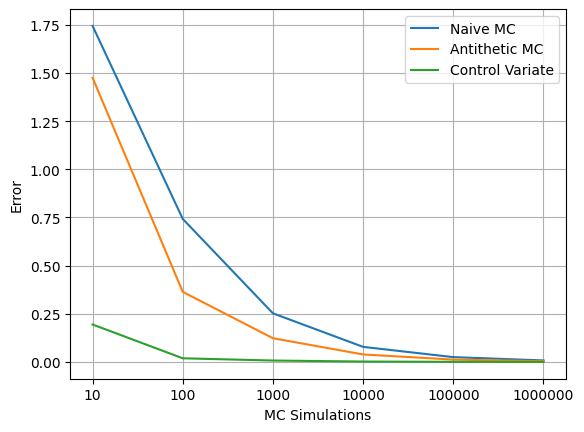
\includegraphics[width=0.4\linewidth]{figures/asian_option_price}
%    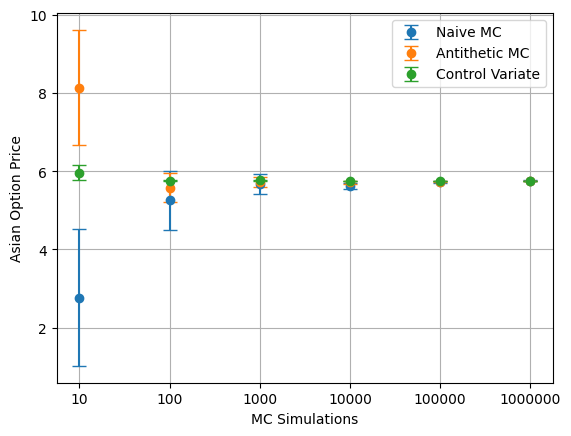
\includegraphics[width=0.4\linewidth]{figures/asian_option_error}
%  \end{center}
%  \caption{The left plot reports the estimated prices as a function of the number of simulated Monte Carlo events for naive, antithetic and control variate techniques.
%    Right plot instead reports the estimate uncertainties.}
%  \label{fig:asian_mc_results}
%\end{figure}
%
%%\section*{Exercises}
%%\input{options_ex_text} % da riguardare
\chapter{Short Rate Models}

The volume of traded interest rate derivatives in both the OTC and exchange-traded markets have been increasing sharply over the past decades. As the number of new and simultaneously exotic interest rate products virtually exploded, it has been a key challenge to find good and primarily robust procedures for pricing and also hedging these products. To reach this goal it is essential to have reliable models to describe the evolution of the interest rate with time.

In this Chapter the most common interest rate modeling techniques are reviewed together with related \texttt{python} applications.

\section{The Short Rate and Term Structure Dynamics}

Bond, option, and other derivative prices depend fundamentally on the stochastic process followed by the short rate $r$ under a risk-neutral probability measure.

Let $Z(t, T)$ be the price at time $t$ of a zero-coupon bond with maturity $T$. The corresponding annualized continuously-compounded yield $R(t, T)$ is defined by the relation:

$$Z(t, T) = e^{-R(t, T)(T-t)} \implies R(t, T) = -\frac{\ln Z(t, T)}{T-t}$$

The \textbf{zero-coupon yield curve} (or term structure of interest rates) represents the collection of these yields across various maturities $T$.

The \textbf{instantaneous short rate} $r(t)$ at time $t$ represents the rate applicable over an infinitesimally short time interval. Analytically, it corresponds to the limit of the yield curve as maturity approaches the current time:

$$r(t) = \lim_{T \to t^{+}} R(t, T)$$

Once the stochastic process for $r(t)$ is fully specified, the theoretical evolution of the entire yield curve is determined. Short-rate models are prized in quantitative finance for their high degree of mathematical tractability and flexibility, often yielding closed-form solutions for zero-coupon bonds and European options.

The risk-neutral evolution of these models is commonly represented by the generalized stochastic differential equation (SDE):

$$dr(t) = \left[\theta(t) - \alpha(t)r(t)\right] dt + \sigma(t)r(t)^{\gamma} dW(t)$$
where $dW(t)$ is a standard Brownian motion under the risk-neutral measure, and $\theta$, $\alpha$, and $\sigma$ are deterministic functions of time governing the drift and diffusion terms.

\subsection{Equilibrium vs. No-Arbitrage}

Short-rate models are generally categorized into two broad philosophical classes based on how they interact with market data:
\begin{itemize}
\item \textbf{Equilibrium Models}: these models originate from fundamental economic assumptions regarding macroeconomic variables and market equilibrium. They derive the short-rate process dynamically, treating the resulting term structure as an output. Consequently, equilibrium models do not automatically fit today’s observed term structure of interest rates verbatim (requiring parameter estimation or market calibration). Examples include the Vasicek and Cox-Ingersoll-Ross (CIR) models, where parameters ($\theta, \alpha, \sigma$) are typically assumed to be time-homogeneous constants.
\item \textbf{No-Arbitrage Models}: these models are explicitly constructed to take today's observed yield curve as an exact input, ensuring that the model prices traded zero-coupon bonds perfectly at $t = 0$ (e.g., Hull-White or Black-Karasinski extensions).
\end{itemize}

A prevalent subset within both categories is represented by \textbf{one-factor models}, in which the stochastic evolution of $r(t)$ is driven by a single Brownian motion $dW(t)$.

By relying on a single source of uncertainty, one-factor models assume that the dynamics of the entire term structure are fully captured by the short rate. While this implies that all yields across different maturities must move in the same direction over any infinitesimal time interval, it does not restrict them to move by the same magnitude.

Although one-factor formulations provide immense analytical tractability, capturing complex yield curve shifts (such as twists and butterflies) often necessitates multi-factor extensions.

\section{Vasicek Model}\label{vasicek-model}

In Vasicek model the process for $r$ is described by

\begin{equation}
	dr = k(\theta - r_t)dt + \sigma dW
	\label{eq:vasicek_process}
\end{equation}
where \(k\), \(\theta\) and \(\sigma\) are constants.

One important difference between interest rates and other stochastic quantities is that interest rates appear to be pulled back to some long-run average level over time. This characteristic is called \emph{mean reversion}. When $r$ is high, mean reversion tends to cause it to have a negative drift; when $r$ is low, mean reversion tends to cause it to have a positive drift.

There are real economic arguments in favor of mean reversion. When rates are high, the economy tends to slow down and there is low demand for funds from borrowers. As a result, rates decline. When rates are low, there tends to be a high demand for funds on the part of borrowers and rates tend to rise.

The Vasicek model incorporates this feature (the short rate is pulled to a level $\theta$ at a rate $k$), which is a good property, but interest rates can go negative, which instead is not such as good property.

\begin{finmarkets}
	The following code implements the \texttt{VasicekModel} referring to the process described by Eq.~\ref{eq:vasicek_process}.
\end{finmarkets}

\pythoncodenon{code/short_rates_vasicek.py}

Figure~\ref{fig:vasicek_path} shows just various realizations of the short rate using the following parameters: $r_0=0.02$, $k=0.3$, $\theta=0.1$ and $\sigma=0.03$. 
Two facts can be noticed by this plot: each process starts at $r_0$, but is pulled towards 0.10 which is the value of $\theta$ (dashed red line), and the interest rate can drop below 0\%. The Figure also shows the expected value of the process.

\begin{figure}[htb]
	\centering
	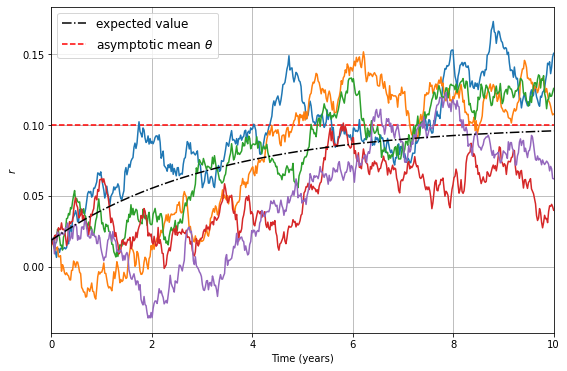
\includegraphics[width=0.7\linewidth]{figures/vasicek_short_rate}
	\caption{A realization of a path determined with Vasicek model ($k=0.3, \theta=0.1, \sigma=0.03$).}
	\label{fig:vasicek_path}
\end{figure}

\subsubsection{Vasicek Stochastic Differential Equation}
\label{vasicek-stochastic-differential-equation}

In this Section we outline the steps necessary to determine the solutions of Eq.~\ref{eq:vasicek_process}.
Multiplying both sides by \(e^{kdt}\) and rearranging the terms gives

\begin{equation*}
	e^{kdt}dr_t + e^{kdt}kr_t dt = e^{kt}k\theta dt + e^{kt}\sigma dW
\end{equation*}
The left-hand side follows the product rule for the derivative

\begin{equation*}
	d(e^{kdt}r_t) = e^{kdt}dr_t + e^{kdt}kr_t dt= e^{kt}k\theta dt + e^{kt}\sigma dW
\end{equation*}
Then we can integrate both sides

\begin{equation*}
	\int^{t=T}_{t=s} d(e^{kdt}r_t)\,dt = \int^T_s e^{kt}k\theta dt +\int^T_s e^{kt}\sigma dW
\end{equation*}
The integral on the left-hand is trivial since \(\int^b_a\,dx = x(b)-x(a)\), so

\begin{equation*}
	e^{kT}r_T - e^{ks}r_s = \int^T_s e^{kt}k\theta\,dt +\int^T_s e^{kt}\sigma\,dW
\end{equation*}
and solving for $r(T)$

\begin{equation*}
	r_T=e^{-k(T-s)}r_s+ e^{-kT}\int^T_s e^{kt}k\theta\,dt +e^{-kT}\int^T_s e^{kt}\sigma dW
\end{equation*}
The second term of the right-hand side is a simple deterministic integral

\begin{equation*}
	e^{-kT}\int^T_s e^{kt}k\theta\,dt=e^{-kT}k\theta\int^T_s e^{kt}d_t=e^{-kT}k\theta\frac{1}{k}(e^{kt}|^T_s)= e^{-kT}\theta(e^{kT}-e^{ks})=\theta\left(1-e^{-k(T-s)}\right)
\end{equation*}
Substituting back we get the searched solution

\begin{equation}
	r_T=e^{-k(T-s)} r_s+\theta(1-e^{-k(T-s)})+ \sigma e^{-kT}\int^T_s e^{kt}\,dW
\end{equation}

The first thing to note is that the short rate is made of a deterministic term
and a stochastic integral.
Therefore, the rate is distributed like a normal Gaussian

\begin{equation*}
	r_T \sim \mathcal{N}(\mathbb{E}(r_t), \textrm{var}(r_t))
\end{equation*}
We can also determine the mean and the variance of such a distribution.
Concerning the mean

\begin{equation}
	\mathbb{E}(r_T)=e^{-k(T-s)} r_s+\theta\left(1-e^{-k(T-s)}\right)
\end{equation}
where the property that $\mathbb{E}(\textrm{stochastic~Integral}) = 0$ has been used.

Regarding the variance, noting that the variance of a deterministic variable is zero, we only need to calculate it for the stochastic integral. We can do this by using the It$\hat{o}$ Isometry, as the terms inside the Stochastic Integral are deterministic functions of time.

\begin{equation*}
	\textrm{var}(r_T)=\mathbb{E}(r^2_T)-(\mathbb{E}(r_T))^2
\end{equation*}
where $(\mathbb{E}(r_T))^2 = 0$ therefore

\begin{equation}
	\begin{aligned}
		\textrm{var}(r_T)&=\mathbb{E}(r^2_T)=\mathbb{E}(\sigma^2 \int^T_s e^{-2k(T-t)}\,dt)=\sigma^2 e^{-2kT} \mathbb{E}( \int^T_s e^{-2k(-t)}\,dt)=\\
		&=\sigma^2 e^{-2kT} \frac {1}{2k}(e^{2kT}-e^{2ks})=\sigma^2 \frac {1}{2k}(1-e^{2k(T-s)}) 
	\end{aligned}
\end{equation}
where we have used that $dW^2 = dt$.
So in conclusion the distribution of the stochastic rate is

\begin{equation}
	r_T \sim \mathcal{N}(e^{-k(T-s)} r_s+\theta(1-e^{-k(T-s)}),\sigma^2 \frac {1}{2k}(1-e^{2k(T-s)}))
\end{equation}

\subsubsection{Bond Pricing Equation}\label{bond-pricing-equation}

Although applied to bonds this kind of technique is more general and may be used to price many other contracts.

Since the whole idea relies on building a hedged portfolio we need to face the technical problem of the lack of an underlying asset with which
to hedge a bond (since it is a ``derivative'' of $r$). The only way to do that is by hedging one bond with another of a different maturity.

So let's set up a portfolio containing two bonds with different maturities $T_1$ and $T_2$ and price respectively $Z_1(r, t, T_1)$
and $Z_2(r, t, T_2)$. We hold one of the former and a number $\Delta$ of the latter

\begin{equation*}
	\Pi = Z_1-\Delta Z_2
\end{equation*}
The change in this portfolio in a time $dt$ is given by

\begin{equation*}
	d\Pi = \cfrac{\partial Z_1}{\partial t}dt + \cfrac{\partial Z_1}{\partial r}dr + \cfrac{1}{2}\sigma^2 \cfrac{\partial^2 Z_1}{\partial r^2}dt - \Delta\left(\cfrac{\partial Z_2}{\partial t}dt + \cfrac{\partial Z_2}{\partial r}dr + \cfrac{1}{2}\sigma^2 \cfrac{\partial^2 Z_2}{\partial r^2}dt\right)
\end{equation*}
where we have applied It$\hat{o}$'s lemma to functions of $r$ and $t$. All the randomness in this expression comes from $dr$ terms given that the rate follows Eq.~\ref{eq:vasicek_process} which contains the Brownian motion $dW$. So to eliminate it (hedging) we need to choose $\Delta$ such that $dr$ terms canceled out

\begin{equation*}
	\Delta = \cfrac{\cfrac{\partial Z_1}{\partial r}}{\cfrac{\partial Z_2}{\partial r}}
\end{equation*}
So we get

\begin{equation*}
	d\Pi = \cfrac{\partial Z_1}{\partial t}dt + \cfrac{1}{2}\sigma^2 \cfrac{\partial^2 Z_1}{\partial r^2}dt - \Delta\left(\cfrac{\partial Z_1}{\partial t}dt + \cfrac{1}{2}\sigma^2 \cfrac{\partial^2 Z_1}{\partial r^2}dt\right) = r\, \Pi dt = r \left(Z_1 - \Delta Z_2\right)dt
\end{equation*}
where we have used arbitrage arguments to set the return of the portfolio equal to the risk-free rate (i.e. this risk-free rate is just the spot rate). Rearranging the terms

\begin{equation*}
	\cfrac{\cfrac{\partial Z_1}{\partial t} + \cfrac{1}{2}\sigma^2 \cfrac{\partial^2 Z_1}{\partial r^2} - rZ_1}{\cfrac{\partial Z_1}{\partial r}}=\cfrac{\cfrac{\partial Z_2}{\partial t} + \cfrac{1}{2}\sigma^2 \cfrac{\partial^2 Z_2}{\partial r^2} - rZ_2}{\cfrac{\partial Z_2}{\partial r}}
\end{equation*}

Since the two sides of the equation depend on $T_1$ and $T_2$ separately the only way for this to be possible is for both sides to be independent of the maturity date. So in general

\begin{equation*}
	\cfrac{\cfrac{\partial Z}{\partial t} + \cfrac{1}{2}\sigma^2 \cfrac{\partial^2 Z}{\partial r^2} - rZ}{\cfrac{\partial Z}{\partial r}}= a(r, t)
\end{equation*}
for some function $a(r, t)$. A convenient definition for $a$ is $a(r, t) = \sigma(r, t)\lambda(r, t)-u(r, t)$ which leads to the bond pricing equation
\begin{equation}
	\cfrac{\partial Z}{\partial t} + \cfrac{1}{2}\sigma^2 \cfrac{\partial^2 Z}{\partial r^2} + (u-\lambda\sigma)\cfrac{\partial Z}{\partial r}-rZ = 0
	\label{eq:bond_pricing_equation}
\end{equation}

The function $\lambda$ is called the market price of risk since it can be interpreted as the excess return above the risk-free rate for accepting a certain level of risk.

\subsubsection{Solution for the Vasicek Model}
\label{solution-for-the-vasicek-model}
The value of a zero-coupon bond according to Eq.~\ref{eq:bond_pricing_equation} in the context of the Vasicek model is

\begin{equation} 
	\begin{gathered}
		Z(0, T) = e^{A(0,T)-r_0 B(0,T)} \\
		B(0, T) = \cfrac{1-e^{-kT}}{k}\\
		A(0, T) = \cfrac{(B(0, T)-T)(k^2\theta - \sigma^2/2)}{k^2} - \cfrac{\sigma^2 B(0, T)^2}{4k}
		\label{eq:zcb_vasicek}
	\end{gathered}
\end{equation}
Furthermore
\begin{equation}
	R(t, T) = \cfrac{1}{T-t} A(t,T)+\cfrac{1}{T-t}B(t, T)r(t)
	\label{eq:term_structure_vasicek}
\end{equation}
showing that the entire term structure can be determined as a function of $r(t)$ once the model parameters have been chosen.

All the formulas discussed in the previous Sections have been implemented in the \texttt{VasicekModel}.
To demonstrate some of the possible curve shapes allowed by the Vasicek model solving Eq.~\ref{eq:zcb}, Figure~\ref{fig:yield_vasicek} shows yield curves with different spot rates. Notice that the yield curve can be both increasing or decreasing with maturity.

\begin{figure}[htb]
	\centering
	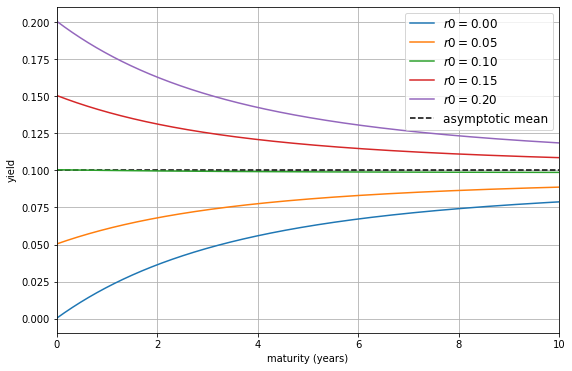
\includegraphics[width=0.7\linewidth]{figures/vasicek_yields}
	\caption{Various yield curves computed according to the Vasicek model ($k=0.3, \theta=0.1, \sigma=0.03$).}
	\label{fig:yield_vasicek}
\end{figure}

Just to cross check the bond pricing formula was implemented correctly, the price using Eq.~\ref{eq:zcb_vasicek} versus the price using Monte Carlo simulation of $\mathbb{E}\left[e^{-\int_0^T r_s ds}\right]$ have been compared. The prices are in excellent agreement.

\pythoncodenon{code/short_rates_vasicek_mc_check.py}
\begin{ioutput}
Exact Vasicek Price: 0.9697
MC Price: 0.9697 +- 0.0002
\end{ioutput}

\subsubsection{Model Calibration}
In order to estimate the Vasicek model parameters from market data, it is possible to discretize the SDE of Eq.~\ref{eq:vasicek_process} as follows
\begin{equation*}
	r_{t=\delta t} = r_t (1-k\delta t) + k\theta\delta t + \sigma \sqrt{\delta t}\mathcal{N}(0,1)
\end{equation*}
which can be rearranged as
\begin{equation}
	r_{t+\delta t} = ar_t + b + \epsilon
	\label{eq:vasicek_regression}
\end{equation}
Equation~\ref{eq:vasicek_regression} can be used in a linear regression (see Section~\ref{sec:linear-regression}) to determine the model parameters as follows
\begin{equation}
	\begin{gathered}
		k = \frac{1-a}{\delta t} \\
		\theta = \frac{b}{1-a} \\
		\sigma^2 = \frac{Var(\epsilon)}{\delta t}
	\end{gathered}
	\label{eq:vasicek_parameters_estimate}
\end{equation}

As an example the Vasicek model has been calibrated on the 3-months Treasury Bills monthly data since 2010 (\href{https://raw.githubusercontent.com/matteosan1/finance_course/develop/input_files/TB3MS.csv}{TB3MS.csv}). Figure~\ref{fig:TB3MS} reports the scatter plot of $r(t)$ vs $r(t+1)$.

\begin{figure}[htb]
	\centering
	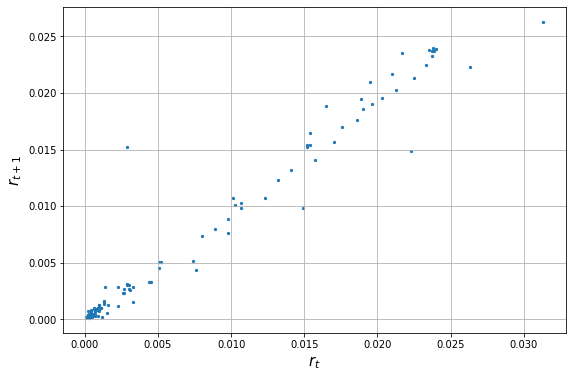
\includegraphics[width=0.7\linewidth]{figures/TB3MS}
	\caption{Scatter plot of 3-months Treasury Bills data since 2010.}
	\label{fig:TB3MS}
\end{figure}

The regression is performed in the following code, notice that it is necessary to remove possible \texttt{NaN} values from the dataframe for the algorithm to work. For a more detailed explanation of the regression summary please look in Sec.~\ref{sec:linear_regression}.
The corresponding Vasicek model parameter values have been estimated using Eqs.~\ref{eq:vasicek_parameters_estimate}, lines 17-20

\pythoncode{code/short_rates_vasicek_calibration.py}

\begin{ioutput}
OLS Regression Results                            
==============================================================================
Dep. Variable:                  TB3MS   R-squared:                       0.964
Model:                            OLS   Adj. R-squared:                  0.964
Method:                 Least Squares   F-statistic:                     3711.
Date:                Wed, 26 Oct 2022   Prob (F-statistic):          1.25e-101
Time:                        07:38:04   Log-Likelihood:                 713.32
No. Observations:                 140   AIC:                            -1423.
Df Residuals:                     138   BIC:                            -1417.
Df Model:                           1                                         
Covariance Type:            nonrobust                                         
==============================================================================
coef    std err          t      P>|t|      [0.025      0.975]
------------------------------------------------------------------------------
const       9.773e-05      0.000      0.625      0.533      -0.000       0.000
prec           0.9478      0.016     60.922      0.000       0.917       0.979
==============================================================================
Omnibus:                      147.784   Durbin-Watson:                   1.043
Prob(Omnibus):                  0.000   Jarque-Bera (JB):             7494.971
Skew:                           3.357   Prob(JB):                         0.00
Kurtosis:                      38.210   Cond. No.                         123.
==============================================================================

k: 0.627, theta: 0.0019, sigma: 0.018
\end{ioutput}

\begin{figure}[htb]
	\centering
	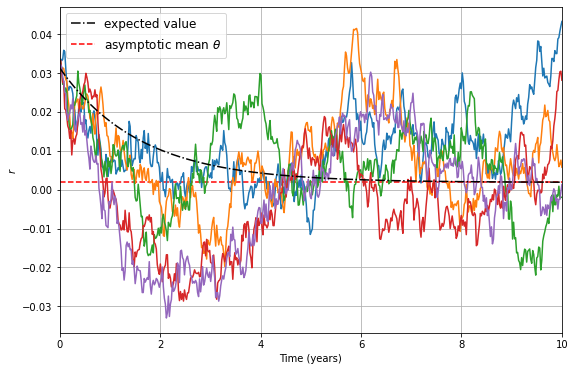
\includegraphics[width=0.7\linewidth]{figures/vasicek_calibrated_paths}
	\caption{Realizations of $r(t)$ with the Vasicek calibrated model ($k=0.63, \theta=0.0019, \sigma=0.018$).}
	\label{fig:vasicek_calibrated_paths}
\end{figure}

\subsection{Cox, Ingersoll and Ross (CIR) Model}
\label{cox-ingersoll-and-ross-cir-model}

In Vasicek model the short term interest rate, $r$ can become negative. In the CIR model this can never happen since the process is expressed as

\begin{equation}
dr = k(\theta - r_t)dt + \sigma\sqrt{r_t}dW
\label{eq:cir_process}
\end{equation}

This has still mean reverting drift but the standard deviation of the change in the short rate in a short period of time is proportional to $\sqrt{r}$. This means that, as the short-term interest rate increases, its standard deviation increases.

In CIR bond prices have similar general form as in Vasicek model $ZBC(0, T)=A(0, T)e^{B(0, T)r_0}$, where

\begin{equation}
B(t, T) = \cfrac{2(e^{\gamma(T-t)}-1)}{(\gamma+k)(e^{\gamma(T-t)}-1)+2\gamma}
\label{eq:cir_B_param}
\end{equation}

\begin{equation}
A(t, T) = \left[\cfrac{2\gamma e^{(k+\gamma)(T-t)/2}}{(\gamma+k)(e^{\gamma(T-t)}-1)+2\gamma}\right]^{2k\theta /\sigma^2}
\label{eq:cir_A_param}
\end{equation}
with $\gamma = \sqrt {k^2 + 2\sigma^2}$. As in the Vasicek model the value of $r(t)$ determines the term structure level at time $t$.

%\begin{finmarkets}
%The following code implements the \texttt{CIRModel} class which has similar methods to \texttt{VasicekModel} for computing short rate, and zero coupon bond value.
%\end{finmarkets}
%
%\pythoncodenon{code/short_rates_cir.py}

Figures~\ref{fig:cir_path} and~\ref{fig:cir_yields} show respectively one simulation of the short rate and the interest rate resulting from the application of the CIR model. Notice how it remains always positive.

\begin{figure}[htb]
\centering
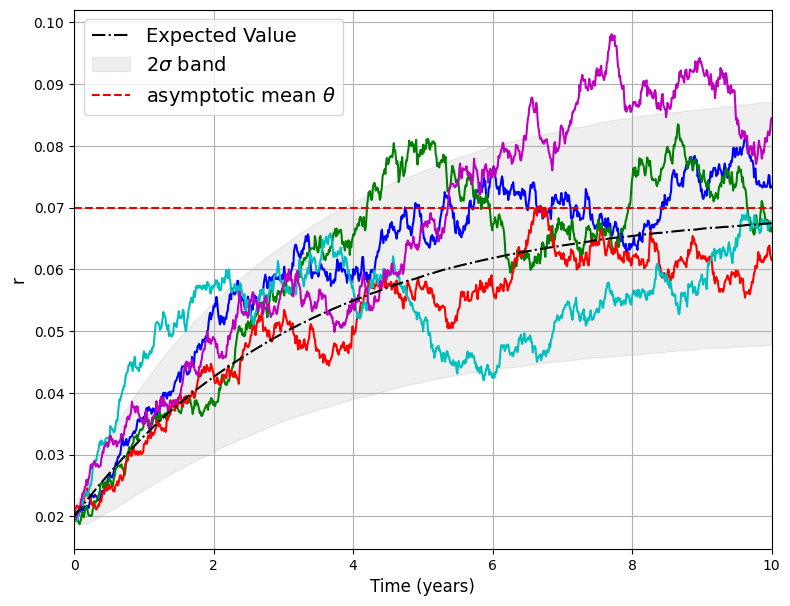
\includegraphics[width=0.65\linewidth]{figures/cir_short_rate}
\caption{Various realizations of short rate determined with CIR model ($k=0.3, \theta=0.07, \sigma=0.03$). The plot shows also the expected value and the $2\sigma$ band.}
\label{fig:cir_path}
\end{figure}

\begin{figure}[htb]
\centering
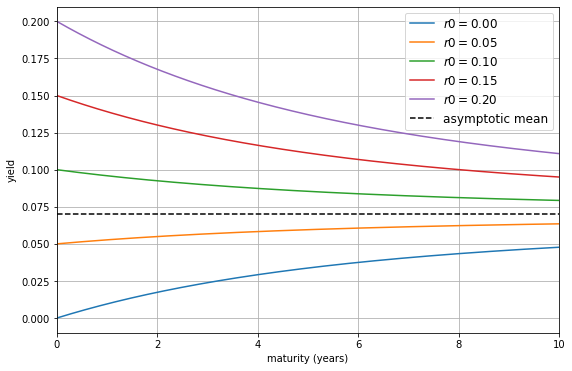
\includegraphics[width=0.65\linewidth]{figures/cir_yields}
\caption{Various yield curves computed according to the CIR model ($k=0.3, \theta=0.07, \sigma=0.03$).}
\label{fig:cir_yields}
\end{figure}

%\section{No-arbitrage Model}
%\label{no-arbitrage-model}
%
%The main disadvantage of the equilibrium, models is that they do not automatically fit today's term structure of interest rates. By choosing the appropriate parameters they can provide an approximate fit to many of the term structures but the fit is not usually exact and in some cases no reasonable fit can be found.
%
%A no-arbitrage model is designed to be exactly consistent with today's term structure of interest rates (i.e.~todas's term structure of interest rate is an input of the model). In this kind of models the drift term is in general dependent on time since the shape of the initial zero curve governs the average path taken by \(r\).
%
%However, in order to fit today’s term structure, the model parameters have to be calibrated to prevailing market data. The calibration process is responsible that a model eventually yields consistent instrument prices. Nonetheless, calibrating a model correctly is somehow burdensome and takes significant additional computing effort.
%
%%\subsection{Ho-Lee Model}\label{ho-lee-model}
%%Ho and Lee [55] did pioneer work by proposing the first no-arbitrage model consistent with the initial term structure. Allowing for time-dependent drift parameters typically makes short rate models consistent with a prevailing set of bond prices. In the continuous-time Ho-Lee model the stochastic process followed by the short rate is [55, 60, p.1020, p.184]
%%
%%This model was presented by Ho and Lee in the form of a binomial tree of
%%bond prices with two parameters: the short rate standard deviation and
%%the market price of risck of the short rate. It has since been shown
%%that the model is
%%
%%\[dr=\theta(t)dt +\sigma dW\]
%%where \(\sigma\), the instantaneous standard deviation of the short
%%rate, is constant and \(\theta(t)\) is a function of time chosen to
%%ensure that the model fits the initial term structure.
%%The variable
%%\(\theta(t)\) defines the average direction that \(r\) moves at time
%%\(t\). This is independent of the level of \(r\).
%%
%%The variable \(\theta(t)\) can be calculated analytically, it is
%%
%%\[\theta(t)=F_t(0, t) + \sigma^2 t\]
%%
%%where \(F(0, t)\) is the instantaneous forward rate for the maturity
%%\(t\) as seen at time zero and the subscript \(t\) denotes a partial
%%derivstive with respect to \(t\). As an approximantion \(\theta(t)\)
%%equals \(F_t(0, t)\). This means that the average direction that the
%%short rate will be moving in the future is approximately equal to the
%%slope of the instantaneous forward curve.
%%Similar to the Vasicek model, for every t there is a positive probability that the interest rates become negative.
%%
%%Applying Itˆo’s lemma, the SDE (6.9) can be solved explicitly for bond prices and short rates. There is an explicit formula available in the Ho-Lee model and thus the term structures are defined as
%%
%%In Ho-Lee model bond price can be determined analytically
%%
%%\[Z(t, T)=A(t, T)e^{-r(t)(T-t)}\]
%%where
%%
%%\[\ln A(t, T)=\ln\cfrac{Z(0,T)}{Z(0,t)}+(T-t)F(0,t)-\cfrac{1}{2}\sigma^2 t(T-t)^2\]
%%
%%In these equations, time zero is today, Times \(t\) and \(T\) are
%%general times in the future with \(T\geq t\). The equations, therefore,
%%define the price of a zero coupon bons at a future time \(t\) in terms
%%of the short rate at time \(t\) and the prices of bonds today. The
%%latter can be calculater from today's term structure.
%
%\subsection{Hull-White Model}
%\label{hull-white-model}
%The unsatisfactory fitting of the observed term structure of interest rates implied by the Vasicek model brought Hull and White~\cite{bib:hull_white_model} in 1990 to propose a new model that basically combines the advantages of the Vasicek and those of no-arbitrage models.
%
%As they defined it, it is an extension of the Vasicek model. However, in H-W the parameters are time dependent, what increases the possibility of calibrating them with respect to market data. The Hull-White model is growing in importance lately due to the reason that it allows the interest rates to be negative while we will not find this feature in many other models. 
%In the past, when the people surrounding the financial world thought of negative interest rates as something impossible, it was criticized for the same reason. However, nowadays reality is quite different and negative rates are all over the market. Furthermore, many specialists on the matter say they are here to stay.
%
%The explanation of why negative interest rates are possible in this model is that the short rate in Hull-White is normally distributed (it is a so-called Gaussian model), therefore:
%\begin{equation}
%dF = σ_N F dW;\quad F(0) = f
%\end{equation}
%where $σ_N$ is the normal volatility. 
%
%The Hull-White stochastic process is defined as
%\begin{equation}
%dr = \left(\theta(t) - a r \right)dt + \sigma dW
%\end{equation}
%where $a$ and $\sigma$ are constants. This can be seen as a pure no-arbitrage model with mean reversion ($a$ is the mean reverting parameter, and is defined in a way in which the drift of the process will be negative for values of $r$ greater than $\theta/a$ and vice-versa) but at the same time, as a Vasicek model with a time-dependent reversion level. Firstly, the Hull-White model makes the parameter $\theta$ time-dependent so that there are enough degrees of freedom to fit the model to the interest rate initial term structure. Here $\theta$ is a deterministic function of time and will be calibrated against the theoretical yield curve. On the other hand, $a$ and $\sigma$ should be chosen to reflect the current and future volatilities of the short-term-interest rate. So like in Vasicek model they can be fitted to the current term structure of interest rates and the current term structure of interest-rate volatility respectively.
%
%We can appreciate it better recalling the Term Structure equation with the Zero Coupon boundary condition and the Hull-White $r$-dynamics:
%\begin{equation}
%\begin{cases}
%\cfrac{\partial F^T}{\partial t} + \left[\theta(t) − a r(t)\right]\cfrac{\partial F^T}{\partial r}
%+\cfrac{1}{2}\sigma^2\cfrac{\partial^2 F^T}{\partial r^2} - r(y)F^T = 0 \\
%F(r, T, T) = 1
%\end{cases}
%\label{eq:HW_PDE}
%\end{equation}
%
%%We see that µ(t, r) − λ(t, r)σ(t) = θ(t) − a(t)r(t) and so, the drift includes the market price of risk and the volatility that should be calibrated against real data. T
%
%The analytical solution for the short rates in this model is as follows:
%\begin{equation}
%r(t) = r(s)e^{−a(t−s)} + \int_{s}^{t}e^{−a(t−u)}\theta(u)du + \sigma\int_s^t e^{−a(t−u)}dW(u)
%\end{equation}
%where
%\begin{equation}
%\theta(t) = f(0, T) + a f(0, T) + \cfrac{\sigma^2}{2a}\left(1 − e^{−aT}\right)
%\end{equation}
%and the Zero-Coupon bond price:
%\begin{equation}
%p(t, T) = A(t, T)e^{B(t,T)r(t)}
%\end{equation}
%\begin{equation}
%A(t, T) = \cfrac{p(0, T)}{p(0, t)}\textrm{exp}\left\{B(t, T)f(0, t) − \cfrac{\sigma^2}{4a}B(t, T)^2\left(1 − e^{−2at}\right)\right\}
%\end{equation}
%\begin{equation}
%B(t, T) = \cfrac{1}{a} \left(1 − e^{−a(T −t)}\right)
%\end{equation}
%with $f(0, t)$ being the forward rate and $p(0, t)$ the price of a bond starting today with maturity at time $t$.
%
%\subsection{Approximate Solution with Finite Difference}
%In this Section we are going to implement the pricing of Zero-Coupon bonds solving the Hull-White PDE through the Finite Difference Method, in particular, Crank-Nicolson~\ref{sec:finite_difference}.
%
%To solve the PDE in Eq.~\ref{eq:HW_PDE} through Crank-Nicolson we then need to define a grid with the rates as rows and time as columns. The idea behind this grid is to discretize these two variables in $N$ pieces of $h$ length equal to $d$r and $T$ pieces of $k$ length equal to $dt$. Therefore, applying the central and second central differences to both variables we get
%\begin{equation}
%\begin{cases}
%u_{i,j} = u(r_i, t_j ) \\[1ex]
%\cfrac{\partial u(r_i, t_j )}{\partial t} = \cfrac{u_{i,j+1} − u_{i,j−1}}{2k} \\[1ex]
%\cfrac{\partial u(r_i, t_j )}{\partial r} = \cfrac{u_{i+1,j} − u_{i−1,j}}{2h} \\[1ex]
%\cfrac{\partial^2 u(r_i, t_j )}{\partial r^2}=\cfrac{u_{i+1,j} + u_{i−1,j} − 2u_{i,j}}{h^2}
%\end{cases}
%\end{equation}
%Now, applying these Crank-Nicolson equalities to the Hull-White term-structure Equation~\ref{eq:HW_PDE} we have
%\begin{equation}
%\cfrac{\partial u_{i,j}}{\partial t} = r_i u_{i,j} − \left(\theta(t) − ar(t)\right) \cfrac{u_{i+1,j} − u_{i−1,j}}{2h}
%−\cfrac{1}{2}\sigma^2\cfrac{u_{i+1,j} + u_{i−1,j} − 2u_{i,j}}{h^2}
%\end{equation}
%that can be rearranged to give the multipliers of each $u_{i,j}$
%\begin{equation}
%\cfrac{\partial u_{i,j}}{\partial t} = \left(-\cfrac{\sigma^2}{2h^2}+ \cfrac{\theta(t) − a r(t))}{2h}\right)
%u_{i−1,j}+\left(\cfrac{\sigma^2}{h^2}+r_i\right)u_{i,j}−\left(\cfrac{\sigma^2}{2h^2}+ \cfrac{\theta(t) − a r(t))}{2h}\right)
%u_{i+1,j}
%\end{equation}
%Thus, letting:
%\begin{equation}
%\begin{cases}
%P_d = −\cfrac{\sigma^2}{2h^2} + \cfrac{\theta(t) − ar(t)}{2h} \\[1ex]
%P_m = \cfrac{\sigma^2}{h^2}+r_i \\[1ex]
%P_u = \cfrac{\sigma^2}{2h^2}+ \cfrac{\theta(t) − a r(t))}{2h}
%\end{cases}
%\end{equation}
%we can perform the following matrix where $t_j = jk; j = 0, 1, 2, \ldots , T$ and $r_i =ih; i = 0, 1, 2, \ldots, N$
%\begin{equation}
%A =
%\begin{bmatrix}
%P_m(r_0, t_j) & P_u(r_0, t_j) & 0 & 0 & 0 & \cdots & 0 \\
%P_d(r_1, t_j) & P_m(r_0, t_j) & P_u(r_0, t_j) & 0 & 0 & \cdots & \vdots \\
%0 & P_d(r_2, t_j) & P_m(r_2, t_j) & P_u(r_2, t_j) & 0 & \cdots & \vdots \\
%0 & 0 & P_d(r_3, t_j) & P_m(r_3, t_j) & P_u(r_3, t_j) & \cdots & \vdots \\
%\vdots & \vdots & \vdots & \vdots & \vdots & \vdots & \vdots \\
%0 & 0 & 0 & \cdots & 0 & P_d(r_N, t_j) & P_m(r_N, t_j) 
%\end{bmatrix}
%\end{equation}
%that will define the behavior of the rates every time-step $k$ passes. Letting a vector $\mathbf{u}$ represent the rates at time $j$, following Crank-Nicolson, we will have the functions that define increments in rates from $j$ to $j + 1$ as:
%\begin{equation}
%\cfrac{\mathbf{u}_{j+1} − \mathbf{u}_j}{k}=\cfrac{[A](tj)\mathbf{u}_j + [A](t_{j+1})\textbf{u}_{j+1}}{2}
%\end{equation}
%that will be solved as:
%\begin{equation}
%\textbf{u}_j = \left([I] + \cfrac{k}{2}[A](t_j)\right)^{-1}\left([I] − \cfrac{k}{2}[A](t_{j+1})\right)\mathbf{u}_{j+1}
%\end{equation}
%
%Reprocessing this calculations starting from maturity backwards for all timesteps and organizing $\mathbf{u}$ in a matrix we will get the solution for the PDE. 
%
%As we are pricing Zero-Coupon bonds, at maturity our derivatives will be worth 1. Therefore, the first boundary condition for this system of equations will be $\mathbf{u}^T = 1$ for all $i$.
%
%On the other hand, $\cfrac{\partial^2 u(r_i, t_j )}{\partial r^2}=0$ is used as boundary conditions at the first step of the grid ($P_d(r_0, t_j )$, $P_m(r_0, t_j )$ and $P_u(r_0, t_j )$).
%
%%6.3 Forward rate models
%%6 Term structure modeling
%%Forward rate models describe the arbitrage-free dynamics of the term structure of interest rates through the evolution of forward rates f (t, T ). The distinguishing feature of these models is that they explicitly describe the evolution of the full term structure, contrary to the previously discussed short rate models, which do only provide a description of the dynamics of the short rate r(t) [46, p.149]. Instantaneous short rate models, as we have seen before, are mostly easy to implement and are usually able to price many standard and also nonstandard interest rate derivatives consistently [56, p.679].
%%However, to legitimize the application of forward rate models, there are the two major limi- tations of short rate models that are generally overcome by using different types of forward rate models:
%%- In short rate models the current value of all term structure quantities is solely determined by the current value of the short rate. Thus, the term structure is entirely summarized by today’s short rate. In multifactor models the complexity of the yield curve dynamics is subsumed into the current values of a finite, but usually small number of underlying factors [46, 56, p.149, p.679f]. The new generation of correlation-dependent instruments, however, requires models that describe the state of the world by the full term structure and not necessarily by a finite number of factors, which are often not able to deal with this new dimension of complexity [92, p.311].
%%- Short rate models do not provide us with a complete freedom in the choice of the corre- sponding volatility structure. In a forward rate framework the forward rate dynamics are completely specified through their instantaneous volatility structure. In contrast, in short rate models the volatility of the short rate alone is not sufficient to fully characterize the relevant interest rate model [20, 56, 92, p.183, p.679, p.311f].
%%Forward rate models can basically be divided into two classes, namely models based on con- tinuous and simple rates, respectively. The by far most popular continuous forward rate model is the Heath, Jarrow and Morton framework. It was one of the first forward rate models pro- posed and simultaneously establishes a basis for models based on simple rates. These models are therefore closely related to the Heath, Jarrow and Morton approach and called LIBOR market models. The seemingly minor shift from continuous to simple rates has surprisingly far-reaching practical and theoretical implications [46, p.165f], as we will see later on. As in the application of both models, Heath–Jarrow–Morton as well as LIBOR market model, Monte Carlo tech- niques play a decisive role, we will give these two approaches a fundamental treatment and will implement them in Section 7 and 8, respectively.
%%52
%%
%%7 Heath, Jarrow and Morton
%%In 1992 Heath, Jarrow and Morton (hereafter, HJM) published the important paper Bond pricing and the term structure of interest rates [53] describing an alternative framework for modeling the term structure of interest rates. Under the risk-neutral measure, they derived a generalized formula for the drifts of instantaneous forward rates in terms of the volatilities of the forward rates. One of the key insights of this framework is that the HJM model is completely defined by specifying the volatilities of forward rates. Consequently, by using the observed term structure of forward rates as an input one can easily match a HJM model with the current market discount bond prices [6, p.310]
%%Basically, there are two common formulations of the model. Firstly, the price based and secondly the forward based approach. The former technique is based on the dynamics of discount bonds, i.e. it takes them as the fundamental building block. The latter directly obtains the no- arbitrage SDE which is obeyed by the forward rates [92, p.314]. For a rigorous proof of the equivalence of these two approaches it is referred to the paper of Carverhill [27]. Note, though, that, historically, the pioneering results of the HJM were first achieved in the forward rates context.
%%The virtue of the HJM theory lies in the fact that within such a framework virtually any (exogenous term structure) interest rate model can be derived. Even market models (see Section 8), for instance, have evolved starting from the instantaneous forward rate dynamics of the HJM approach. However, the disadvantage is that there are only a few volatility structures which lead to a corresponding short rate process which is indeed Markovian. This means that models of this form will, except for some wise choices of volatility specifications, which we will look at in Section 7.2, generally be path-dependent and thus non-Markovian processes [6, 20, p.310, p.184]. A short rate process can be characterized as being Markovian if its future evolution is in no way affected, in a stochastic sense, by its past realizations. If a process is indeed not influenced by its past, then the short rate process is, to use Carverhill’s [26] apt oxymoron, randomly determined [92, p.347f].
%%In general, prices of fixed-income instruments, e.g. bonds, do not depend on the values of a few individual factors but rather on the entire history of the forward rate process. This fact makes computation exceptionally difficult and often only possible by simulation since the nodes of non-recombining, or bushy trees grow exponentially and therefore the approximating lattice will literally explode already after a small number of steps [6, p.310]. As a result, Monte Carlo simulation is the computational tool of choice in the HJM setting.
%%7.1 Framework
%%As mentioned before, the HJM characterizes the dynamics of the entire forward rate curve f (t, T ), whereas 0 ≤ t ≤ T ≤ τ . The origin of any consistent implementation of the HJM approach is the current yield curve, which is obviously based on market data. This yield curve can be described either by the collection of discount bonds P(0,T) or by the instantaneous
%%forward rates f (t, T ). The forward rate at time t for date T > t is defined by [46, 53, 92, p.150, p.79, p.314]
%%∂lnP(t,T) ∂T
%%By solving the differential equation of Expression (7.1) the relationship between forward rates, spot rates and bond prices become obvious. In particular, spot rates, r(t,T), and bond prices, P(t,T), are written in terms of forward rates, f(t,T), as
%%and
%%r(t, T ) = P(t,T) = exp −
%%f(t,T) = −
%%. (7.1)
%%1T T−tt
%%f (t, s)ds 
%%f(t,s)ds ,
%%
%%respectively, for all T ∈ [0,τ], t ∈ [0,T] [6, 53, 92, p.310, p.80, p.314]. Note that the spot rate at time t, r(t), is exactly the same as the instantaneous forward rate at time t for date t, i.e., r(t) = f (t, t) [53, p.80].
%%In the HJM setting, the dynamics of the instantaneous forward rate curve are specified, under a given measure, through the SDE [46, 53, 60, p.150, p.80f, p.200]
%%df(t,T) = α(t,T,ω)dt+σ(t,T,ω)dW(t), (7.4)
%%where ω is a vector containing the past and present values of interest rates as well as bond prices at time t in the sample space Ω. The process W is a standard d-dimensional Brownian motion, whereas d is the number of factors or volatility curves which describe the forward rates. Thus, the HJM approach can be constructed as a one factor as well as a multifactor model.
%%Due to the absence of arbitrage, requested by the no-arbitrage condition, asset prices must
%%be martingales when divided by the numeraire, which in this case is exp 0t r(s)ds. However,
%%forward rates and asset prices are by no means the same. Therefore, the restrictions imposed
%%on the dynamics in (7.4) with the purpose to avoid any arbitrage opportunities are different.
%%Nevertheless, asset prices, particularly bonds, serve as a starting point in order to find theset
%%restrictions. To ensure that the discounted bond prices P (t, T ) exp − r(s)ds are positive
%%0
%%martingales, Heath et al. [53, p.81f] derived the dynamics of the form dP(t,T)
%%P(t,T) =r(t)dt+v(t,T,ω)dW(t), (7.5)
%%where 0 ≤ t ≤ T ≤ τ [46, 60, p.151, p.200]. The volatilities of the bonds v(t, T, ω) may either be functions of observed bond prices or, equivalently, of current forward rates since (7.1) indicates that they are one-to-one related to each other. Applying Itˆo’s formula yet again, Heath et al. showed [53, p.80ff] that forward rate volatilities may be derived from bond price volatilities and we therefore must have
%%∂ ∂T
%%σ(t,T,ω) = − 54
%%v(t,T,ω)
%%and T
%%v(t, T, ω) = − σ(t, s)ds + constant, (7.6)
%%t
%%simultaneously [46, p.152]. Notice, however, that P (t, T ) approaches 1 as t → T and therefore we must have v(T,T,ω) = 0 because bond’s price volatility declines to zero at maturity [92, p.318]. Thus the constant in Equation (7.6) is zero which allows us to rewrite the expression for α as [20, 46, 60, p.186, p.152f, p.200f]
%%
%%α(t, T, ω) = σ(t, T, ω) σ(t, s)ds = σi(t, T, ω) σi(t, s)ds. (7.7)
%%t i=1 t
%%This expression represents the risk-neutral drift imposed by the no-arbitage condition. Addition- ally, (7.7) reveals a key result of the HJM research activities. The assumption of arbitrage-free dynamics has led to a specific relationship between the drift and the volatility. Namely that the drift of the dynamics in (7.4) is completely determined by the volatility structure of the instantaneous forward rates. Thus we know that the HJM drifts themselves are simply a function of the volatilities, either of forward rates, or of discount bonds. If we substitute (7.7) into (7.4) then the new HJM dynamics are [46, 53, 92, p.152, p.89f, p.318ff]
%%
%%df(t,T)= σ(t,T,ω) σ(t,s)ds dt+σ(t,T,ω)dW(t). (7.8)
%%t
%%This SDE defines the no-arbitrage dynamics of the forward rate curve under the risk-neutral measure and is simultaneously the central insight of the HJM approach. Recall why the model eventually fulfills the required no-arbitrage condition. While deriving the forward rate restriction (7.7) and the corresponding dynamics (7.8), a proper specification of the drift was chosen in order to guarantee the absence of arbitrage, or more precisely, to make the discounted bond prices martingales. However, integrating (7.8) leads to the dynamics of f(t,T
%%f(t,T) = f(0,T)+ σ(u,T,ω) σ(u,s)dsdu+ σ(s,T,ω)dW(s), (7.9)
%%0u0
%%which are completely determined once the vector volatility function σ is specified [20, 53, p.186, p.89f]. Only a small step takes us now from the dynamics of the forward rates to the dynamics of the zero coupon bond price P(t,T):
%%dP(t,T)=P(t,T) r(t)dt− σ(t,s)ds dW(t) , (7.10)
%%t
%%where r(t) denotes the instantaneous short term interest rate at time t. The dynamics of r(t) are given by [20, 53, p.186, p.90]
%%
%%r(t) = f (t, t) = f (0, t) + σ(u, t, ω) σ(u, s)ds du + σ(s, t, ω)dW (s). (7.11)
%%0u0
%
%%The decisive discrepancy between HJM and previously discussed instantaneous short rate models has become apparent. We know that the HJM drift is determined once the volatility is finally specified. In contrast, the derivation of the short rate models disclosed that their dynamics and thus their drift parameters could be completely specified independent of any diffusion coefficients. Even though no volatility structures were taken into account, there was still no arbitrage introduced. A wise choice of the drift parameters is indeed crucial for calibrating short rate models to the observed bond prices. Provided that the initial forward rate curve is chosen in a way that the consistency, implied by (7.1), is guaranteed, the HJM model, however, is automatically calibrated to prevailing bond prices. To conclude, while calibrating a HJM model the initial forward curve conditions rather than individual parameters are essential. With regard to the calibrating process of a HJM framework itself, the main effort lies in choosing σ properly to firstly match bond prices and eventually the market prices of interest rate derivatives [46, 60, 92, p.153, p.200, p.312f].
%%7.2 Volatility functions
%%The proceeding section has already foreshadowed that the consequences of the choice of volatility specification for the implementation and simulation of a HJM model are enormous. The short rate process (7.11) is, as mentioned before, not a Markov process in general. However, there are suitable specifications of the volatility function σ(t, T, ω) for which r(t) is yet Markovian [20, 60, p.186f, p.203f]. For an extensive treatment of Markovian short rate processes it is referred to either the paper of Carverhill [26] or the Chapter 16 of Rebonato [92, p.347-359]. In the general case when σ(t,T,ω) is not Markovian, we may encounter major computational problems when discretizing the Dynamics (7.11) for the pricing of even simple derivatives. However, several standard Markovian functional forms for σ(t,T,ω) have been explored. Two of them, both single factor models (d = 1), are listed and shortly explained below [60, p.203]:
%%- Constant σ: σ(t, T, ω) ≡ σ.
%%In this one factor model with constant volatility each increment dW(t) moves the entire forward curve, i.e. all existing points on the curve, by an equal amount of σdW(t). Thus, the forward curve is constrained to move only in parallel [46, p.153]. For this particularly simple specification, bond prices are assumed to be lognormal and all forward rates are normal and exhibit exactly the same volatility. If these distributional assumptions are fulfilled, the according models are qualified as Gaussian [92, p.317f]. They are analytically well-tractable but also unrealistic to some extent, what we will see later on. If we insert σ into Equation (7.7) the resulting drift of a HJM model with constant σ has the form [46, p.153]
%%T
%%α(t, T, ω) = σ σ ds = σ2(T − t).
%%t
%%Solving (7.8) with constant σ leads to the dynamics of the forward rates f(t,T)=f(0,T)+ 12σ2[T2 −(T −t)2]+σW(t),
%%which is simultaneously the continuous-time equivalent of the Ho-Lee model [60, 92, p.202, p.318].
%%Flesaker [40] conducted an empirical test about the constant volatility version of the HJM model for Eurodollar futures and futures options. He found that this general version of the HJM model is unable to explain cross-sectional pricing pattern of futures options and that it exhibits systematic biases, why the model is eventually soundly rejected. Moreover, he observed that the model tends to overvalue short-term options relative to long-term options. Accordingly, he clearly motivated further empirical studies of HJM models where the volatility is allowed to vary over time rather than artificially kept constant.
%%-Exponentialσ: σ(t,T,ω)=σexp(−λ(T−t)),forsomeconstantsσ,λ>0.
%%This diffusion term σ(t,T,ω) has a greater impact on forward rates for short maturities than on forward rates for long maturities [46, p.154]. Due to this fact the HJM model in- cluding an exponential σ is eventually completely equal to the general short rate dynamics proposed by Hull and White [57], see (6.11). This makes clear that one can establish a one-to-one equivalence between the HJM one factor model and the general formulation of the Gaussian one factor instantaneous short rate model of Hull and White [20, p.187].
%%This volatility specification keeps its analytical tractability but is able to perform slightly better than the HJM model with constant σ. Yet, the results are still unsatisfactory and therefore the HJM model including exponential volatility is also rejected [60, p.203].
%%Asides from many standard approaches with the goal of finding suitable specifications of σ(t,T,ω), which make the short rate process indeed Markovian, there have been developed some more sophisticated techniques, too. They basically exploit that, even though a short rate process might not be Markovian, there may yet exist a higher-dimensional Markov process that possesses the instantaneous short rate as one of its components [20, p.188]. Ritchken and Sankarasubramanian [95], for instance, proposed a model for simply capturing the path dependence of the short rate r(t) through a single statistic. In particular, they found a few necessary and sufficient conditions which are imposed on the volatility structure of the forward rates. These conditions enable them to control the short rate’s path dependence and make them analytically tractable [20, 60, p.189, p.205].
%%A second model, which was proposed by Mercurio and Moraleda [78], derives an interest rate model within the HJM framework which explicitly assumes a humped volatility structure in the instantaneous forward rate dynamics and thus is also analytically tractable. They motivate their assumption of a humped volatility structure by the fact that forward rates themselves commonly exhibit humped volatility functions that are generally implied by simple market quotes. They have shown that their model consequently outperforms similar existing models, which do not explicitly contain such a humped shape in volatilities [20, 78, p.191f, p.213].
%%      
    
%\section*{Exercises}
%\begin{question}
Assume that company A has agreed to pay a 6-month LIBOR and receive a fixed interest rate of 8\% per year (with interest payable every six months) from the face value of \$100 million. Swap is 1.25 years to expire. The interest rates for 3, 9 and 15 months are: 10\%, 10.5\% and 11\% respectively. Assume that interest rates are continuously compounded. The 6-month LIBOR is currently 10.2\%. 

Calculate the value of this swap for company A.
\end{question}


%  Add to \texttt{finmarkets} module a class to valuate swaptions, it should have as attributes the underlying IRS, the swap rate volatility and the question date.
%  The class should have the capability of estimating the payoff of the swaptions both with the Black-Scholes formula and Monte Carlo Simulation.
%\end{question}
%
%\begin{solution}
%	class InterestRateSwaption:
%	def __init__(self, exercise_date, irs):
%	self.exercise_date = exercise_date
%	self.irs = irs
%	def npv_bs(self, discount_curve, libor_curve, sigma):
%	A = self.irs.annuity(discount_curve)
%	S = self.irs.swap_rate(discount_curve, libor_curve)
%	T = (self.exercise_date - discount_curve.today).days / 365
%	d1 = (math.log(S/self.irs.fixed_rate) + 0.5 * sigma**2 * T)
%	/ (sigma * T**0.5)
%	d2 = d1 - (sigma * T**0.5)
%	npv = self.irs.notional * A * (S * scipy.stats.norm.cdf(d1) -
%	self.irs.fixed_rate * scipy.stats.norm.cdf(d2))
%	return npv
%	
%	def npv_mc(self, discount_curve, libor_curve, sigma, n_scenarios=10000):
%	A = self.irs.annuity(discount_curve)
%	S = self.irs.swap_rate(discount_curve, libor_curve)
%	T = (self.exercise_date - discount_curve.today).days / 365
%	discounted_payoffs = []
%	for i_scenario in range(n_scenarios):
%	S_simulated = S * math.exp(-0.5 * sigma * sigma * T +
%	sigma * math.sqrt(T) * numpy.random.normal())
%	
%	swap_npv = self.irs.notional * (S_simulated - self.irs.fixed_rate) * A
%	discounted_payoffs.append(max(0, swap_npv))
%	npv_mc = numpy.mean(discounted_payoffs)
%	npv_error = 3 * numpy.std(discounted_payoffs) / math.sqrt(n_scenarios)
%	return npv_mc, npv_error
%\end{ipython}

\begin{question}
Suppose that the LIBOR Forward rates and the discount curve are those defined in
\href{https://github.com/matteosan1/finance_course/raw/develop/libro/input_files/libor_curve.xlsx}{libor\_curve.xlsx} and \href{https://github.com/matteosan1/finance_course/raw/develop/libro/input_files/discount_curve.xlsx}{discount\_curve.xlsx} respectively.
Determine the value of an option to pay a fixed rate of 4\% and receives LIBOR on a 5 year swap starting in 1 year. Assume the notional is 100 EUR, the exercise date is on October, 30th 2020 and the swap rate volatility is 15\%.

\noindent\textbf{Hint:} add \texttt{InterestRateSwap} class to \texttt{finmarkets.py}.
\end{question}

\cprotEnv\begin{solution}
\begin{ipython}
from finmarkets import InterestRateSwap
from datetime import date
from dateutil.relativedelta import relativedelta
from curve_data import discount_curve, libor_curve
from scipy.stats import norm
import math

pricing_date = date.today()
start_date = date.today() + relativedelta(years=1)
exercise_date = date(2020, 10, 30)

irs = InterestRateSwap(start_date, 100, 0.04, 12, 5)
sigma = 0.15
A = irs.annuity(discount_curve, pricing_date)
S = irs.swap_rate(discount_curve, libor_curve, pricing_date)
T = (exercise_date - pricing_date).days / 365
d1 = (math.log(S/irs.fixed_rate) + 0.5 * sigma**2 * T) / (sigma * T**0.5)
d2 = (math.log(S/irs.fixed_rate) - 0.5 * sigma**2 * T) / (sigma * T**0.5)
npv = irs.notional * A * (S * norm.cdf(d1) - irs.fixed_rate * norm.cdf(d2))

print(f"Swaption NPV: {npv:.3f} EUR")
\end{ipython}
\begin{ioutput}
Swaption NPV: 13.587 EUR
\end{ioutput}
\end{solution}


    

\chapter{Interest Rate Derivatives}
\label{interest-rate-swaps-and-swaptions}

In Chapter~\ref{sec:swaps-and-bootstrapping} we introduced the Overnight Index Swap, here we describe the plain vanilla Interest Rate Swap contract and see how it can underlie a Swaption, the European options analogous for interest rate market.

\section{Interest Rate Swaps}\label{sec:interest-rate-swaps}

Interest rate swaps (IRS) consist of two legs. The floating leg pays the reference index fixing at a frequency equal to the floating rate tenor, so for example an IRS on a 3-month EURIBOR will pay a floating coupon every three months.
The fixed leg pays a predetermined cash-flow at annual frequency, regardless of the underlying floating rate tenor (for simplicity we will only consider swaps with maturities which are multiples of 1 year).

The contract parameters are:

\begin{itemize}
\tightlist
\item start date $d_0$;
\item notional $N$;
\item fixed rate $K$;
\item floating rate tenor (months);
\item maturity (years).
\end{itemize}

\subsection{IRS Valuation}
\label{irs-valuation}

Let $d_0^{\mathrm{fixed}},...,d_p^{\mathrm{fixed}}$ be the fixed leg payment dates and $d_0^{\mathrm{float}},...,d_p^{\mathrm{float}}$ be the floating leg payment dates and let's use the following notation:

\begin{itemize}
\tightlist
\item $d$ the pricing date;
\item $D(d, d')$ the discount factor observed in date $d$ for the value date $d'$;
\item $F(d, d', d'')$ the forward rate observed in date $d$ for the period $[d', d'']$;
\item the tenor is $\tau = d' - d$.
\end{itemize}
The NPV of the fixed leg is calculated as follows:

\begin{equation}
\mathrm{NPV}_{\mathrm{fixed}}(d, K) = N\cdot K\cdot\sum_{i=1}^{n}D(d, d_{i}^{\mathrm{fixed}})
\end{equation}
while the NPV of the floating leg is:

\begin{equation}
\mathrm{NPV}_{\mathrm{float}}(d, F) = N\cdot\sum_{i=1}^{m}F(d, d_{j-1}^{\mathrm{float}}, d_{j}^{\mathrm{float}}) \cdot \frac{d_{j}^{\mathrm{float}}-d_{j-1}^{\mathrm{float}}}{360}
\cdot D(d, d_{i}^{\mathrm{float}})
\end{equation}

Therefore the NPV of the swap (seen from the point of view of the counter-party which receives the floating leg) is

\begin{equation}
\mathrm{NPV}(d, F, K) = \mathrm{NPV}_{\mathrm{float}}(d, F) - \mathrm{NPV}_{\mathrm{fixed}}(d, K)
\label{eq:irs_npv}
\end{equation}

For reasons which will become apparent later, it's actually more convenient to express the NPV of an IRS as a function of the fair value fixed rate $S$ of the IRS, also known as the \textbf{swap rate}, which is the value of $K$ which makes $\mathrm{NPV}=0$. On the basis of the previous expressions, we can easily calculate $S$ as

\begin{equation}
\begin{gathered}
\mathrm{NPV}_{\mathrm{fixed}}(d, S) = \mathrm{NPV}_{\mathrm{float}}(d, F)\\[5pt]
N\cdot S\cdot\sum_{i=1}^{n}D(d, d_{i}^{\mathrm{fixed}}) = N\cdot\sum_{i=1}^{m}F(d, d_{j-1}^{\mathrm{float}}, d_{j}^{\mathrm{float}}) \cdot \frac{d_{j}^{\mathrm{float}}-d_{j-1}^{\mathrm{float}}}{360} \cdot D(d, d_{i}^{\mathrm{float}})\\[5pt]
S=\frac{\sum_{i=1}^{m}F(d, d_{j-1}^{\mathrm{float}}, d_{j}^{\mathrm{float}}) \cdot \frac{d_{j}^{\mathrm{float}}-d_{j-1}^{\mathrm{float}}}{360}
\cdot D(d, d_{i}^{\mathrm{float}})}{\sum_{i=1}^{n}D(d, d_i^{\mathrm{fixed}})}
\end{gathered}
\end{equation}

Once we have calculated $S$, we can express the $\mathrm{NPV}$ of an IRS as follows:

\begin{equation}
\begin{split}&\mathrm{NPV}(d, F, K) = \mathrm{NPV}_{\mathrm{float}}(d, F) - \mathrm{NPV}_{\mathrm{fixed}}(d, K) = \\
&= \underbrace{\mathrm{NPV}_{\mathrm{float}}(d, F) - \mathrm{NPV}_{\mathrm{fixed}}(d, S)}_{\textstyle\mathrm{=0}} + \mathrm{NPV}_{\mathrm{fixed}}(d, S) - \mathrm{NPV}_{\mathrm{fixed}}(d, K) \\
& = N\cdot(S-K)\cdot\underbrace{\sum_{i=1}^{n}D(d, d_{i}^{\mathrm{fixed}})}_{\textstyle \mathrm{annuity}}
\end{split}
\label{eq:irs_npv2}
\end{equation}

\begin{finmarkets}
Now we analyze the \texttt{InterestRateSwap} class which allows to valuate IRS contracts. Its attributes are all the parameters needed to define an Interest Rate Swap, also it has methods to compute the annuity, the swap rate and the NPV of the contract.
\end{finmarkets}

\pythoncodenon{code/ir_derivatives_irs.py}

For convenience the relevant inputs that will be used later (forward rate and discount curve definitions) have been saved in \href{https://github.com/matteosan1/finance_course/raw/master/input_files/euribor_curve.xlsx}{euribor\_curve.xlsx} and \href{https://github.com/matteosan1/finance_course/raw/master/input_files/discount_factors_2022-10-05.xlsx}{discount\_factors\_2022-10-05.xlsx} respectively.

Let's test our class instantiating an IRS with 1M notional, 2.3\% fixed rate, 3 months tenor and a maturity of 4 years.

\pythoncodenon{code/ir_derivatives_2.py}

\begin{ioutput}
32807.53
\end{ioutput}
\textbf{Can you guess what could be the \textbf{swap rate} given the NPV obtained above ?}
\noindent
From Eq.~\ref{eq:irs_npv} and since the actual NPV value is positive it is clear that, NPV$_{\textrm{fixed}}$ has to increase with an higher fixed rate to balance the value of NPV$_{\textrm{float}}$.
Alternatively looking at Eq.~\ref{eq:irs_npv2}, $N$ and the annuity are positive so has to be $S > K$ to match the positive sign of the left hand side.
Below we verify that our conclusion was correct and check that a new swap defined with the fixed rate equal to the swap rate just computed has null NPV.

\begin{ipythonnon}
swap_rate = irs.swap_rate(dc, fr)
print (swap_rate)

irs_new = InterestRateSwap(nominal, start_date, maturity,
                           swap_rate, tenor, side="Payer")
print (irs_new.npv(dc, fr))
\end{ipythonnon}
\begin{ioutput}
0.03172845078751083
0.0
\end{ioutput}
\noindent
The result will be as close to zero as the accuracy of the swap rate used in the definition of the new IRS.

%\section{Inheritance Again}
%\begin{finmarkets}
%Now that we have introduced two kinds of swap we can try to make an alternative implementation of their classes, this time using inheritance.
%
%The base (or parent) class will be \texttt{GenericSwap} and it will implement just a constructor with the attributes given by the basic characteristics of a swap: notional, maturity, tenor and rate of the fixed leg.
%\end{finmarkets}
%
%\begin{ipython}
%from finmarkets import generate_dates
%
%class Swap:
%    def __init__(self, start_date, notional, rate_l1, rate_l2,
%                 tenor_months_l1, tenor_months_l2, maturity_years):
%        self.notional = notional
%        self.rate_l1 = rate_l1
%        self.rate_l2 = rate_l2
%        self.dates_l1 = generate_dates(start_date, 12 * maturity_years,
%                                       tenor_months_l1)
%        self.dates_l2 = generate_dates(start_date, 12 * maturity_years,
%                                       tenor_months_l2)
%
%    def npv_l1(self, dc):
%        val = 0
%        for j in range(1, len(self.dates_l1)):
%            F = self.rate_l1.forward_rate(self.dates_l1[j], self.dates_l1[j-1])
%            tau = (self.dates_l1[j] - self.dates_l1[j-1]).days / 360
%            P = dc.df(self.dates_l1[j])
%            val += F * tau * P
%        return val
%
%    def npv_l2(self, dc):
%        val = 0
%        for i in range(1, len(self.dates_l2)):
%            tau = (self.dates_l2[i] - self.dates_2[i - 1]).days / 360
%            val += dc.df(self.dates_l2[i]) * tau
%        return self.notional * self.rate_l2 * val
%
%    def npv(self, dc):
%        return self.npv_l1(dc) - self.npv_l2(dc)
%
%class OvernightIndexSwap(Swap):
%    def npv_l1(self, dc):
%        return self.notional * (dc.df(self.dates_l1[0]) - dc.df(self.dates_l1[-1]))
%
%class InterestRateSwap(Swap):
%    def annuity(self, dc):
%        a = 0
%        for i in range(1, len(self.dates_l2)):
%            a += dc.df(self.dates_l1[i])
%        return a
%
%    def swap_rate(self, dc):
%        num = self.npv_l1(dc)
%        return num / self.annuity(dc)
%
%    def npv(self, dc):
%        S = self.swap_rate(dc)
%        A = self.annuity(dc)
%        return self.notional * (S - self.rate_l2) * A
%\end{ipython}
%\begin{finmarkets}
%This is just an example. Actually may be an overkill to use inheritance here, since there is not much code to share between the classes (the implementation of the NPV calculation is different in each of them). Anyway this is a practical application to show how it works.
%\end{finmarkets}

\section{Swaptions}
\label{interest-rate-swaptions}

Swaptions are the equivalent of European options for the interest rate market. \emph{They give the option holder the right but not the obligation to enter into an interest rate swap at a predetermined fixed rate at the exercise date $d_{ex}$}.

Clearly the option holder will only choose to do this if the underlying swap NPV at $d_{ex}$ is positive. Looking at the expression of the IRS NPV in terms of the swap rate $S$ therefore, we can see that the payoff of the swaption is

\begin{equation}
\mathrm{payoff} = N\cdot \mathrm{max}(0, S(d_{\mathrm{ex}}) - K)\cdot\sum D(d, d_i^{\mathrm{fixed}})
\label{eq:swaption_payoff}
\end{equation}

\subsection{Swaption Valuation}

In order to valuate the swaption payoff the key issue is to estimate $S(d_{\mathrm{ex}})$ and it will be done with two alternative approaches.

\subsubsection{Evaluation through Black Formula}
\label{evaluation-through-black-scholes-formula}

In this case we are going to use (but not to derive) a generalization of the Black formula

\begin{equation}
\mathrm{NPV} = N\cdot A\cdot [S \Phi(d_+) - K\Phi(d_-)]
\end{equation}
where $\Phi$ represents the cumulative distribution function of the normal distribution and

\begin{equation}
\begin{gathered}
d_{\pm} = \frac{\mathrm{log}(\frac{S}{K}) \pm \frac{1}{2}\sigma^{2}T}{\sigma\sqrt{T}}\qquad(\sigma~\textrm{is the volatility of the swap rate})\\
A = \sum_{i=1}^{p}D(d, d_{i}^{\mathrm{fixed}})\qquad\mathrm{(annuity})
\end{gathered}
\end{equation}

\subsubsection{Valuation through Monte Carlo Simulation}
\label{evaluation-through-monte-carlo-simulation}

When pricing swaptions via Monte Carlo simulation, two primary modeling philosophies can be adopted:

\begin{enumerate}
	\item \textbf{Direct Swap-Rate Modeling (Black-Type Framework):} under this approach, one models the target swap rate directly. Starting from the current swap rate $S(d)$ evaluated at the pricing date $d$, we assume it follows a log-normal stochastic process with zero drift under the corresponding forward measure. Its distribution at the exercise date $d_{\mathrm{ex}}$ (with time-to-maturity $T = d_{\mathrm{ex}} - d$) is given by:
	\begin{equation*}
		S(d_{\mathrm{ex}}) = S(d)\exp\left(-\frac{1}{2}\sigma^{2}T+\sigma \sqrt{T}Z\right)
	\end{equation*}
	where $Z\sim\mathcal{N}(0,1)$ and $\sigma$ represents the Black volatility. This method is the industry standard for European swaptions because it matches market quotation conventions directly and requires no modeling of the entire term structure.	
	\item \textbf{Short-Rate Modeling (Equilibrium or No-Arbitrage Framework):} alternatively, one can simulate the evolution of the instantaneous short rate $r(t)$ (such as through the Vasicek model). By generating paths for $r(t)$, we dynamically determine the entire term structure of zero-coupon bond prices, which in turn allows us to price the underlying swap's legs and evaluate derivative payoffs consistently across different maturities and complex exercise structures.
\end{enumerate}

While direct log-normal simulation of the swap rate is computationally efficient and practical for European-style options, the implementation chosen for pedagogical purposes in this text relies on the Vasicek short-rate model. Simulating the short rate directly provides a unified framework: it demonstrates to students how a single foundational stochastic process can simultaneously govern term structure dynamics, yield curve shapes, bond pricing equations, and derivative valuation.

\begin{finmarkets}
The \texttt{finmarkets} module has a class, \texttt{Swaption}, capable of valuing swaptions both with Monte Carlo simulation and Black-Scholes formula. As usual its attributes are the parameters needed to define the swaption itself and the underlying IR swap.
\end{finmarkets}

\pythoncodenon{code/ir_derivatives_3.py}

As an example let's consider a swaption expiring in 1 year whose underlying is a 6 months IRS with a notional of 1~M, fixed rate of 3.5\%, and a maturity of 4 years. In addition we assume a volatility associated to the swap rate of 15\%.
The interest rate are modelled according to the Vasicek model with parameters $a=0.1; b=0.03; \sigma=0.01$ and $r_0=0.02$.
First compute the derivative NPV with the MC simulation estimating also the 95\% confidence level.

\pythoncodenon{code/ir_derivatives_4.py}

\begin{ioutput}
Swaption Price: 58,240.83 +- 981.97 EUR
\end{ioutput}
Figure~\ref{fig:mc_swaption_price} shows the distribution of the simulated swaption prices.

\begin{figure}[htb]
	\centering
	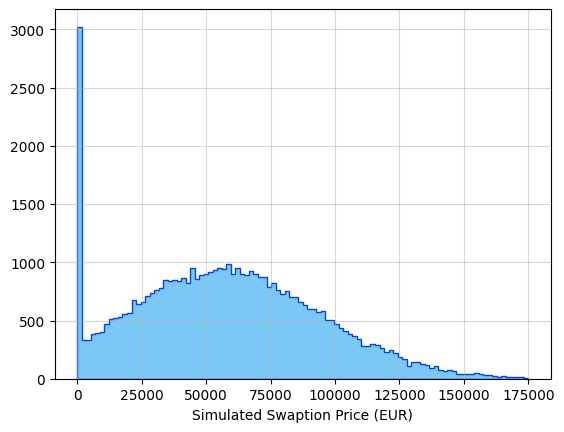
\includegraphics[width=0.55\textwidth]{figures/simulated_swaption_price}
	\caption{Distribution of the simulated swaption prices, the large number of zeros represents simulation with out-of-the-money option.}
	\label{fig:swap_rate}
\end{figure}

Then repeat the pricing using the Black formula; the discount and forward curves are the spot curves estimated with the Vasicek model.

\pythoncodenon{code/ir_derivatives_5.py}
\begin{ioutput}
Swaption Price Black: 57,918.47 EUR
\end{ioutput}
The NPV calculated via the Black formula falls well within the confidence interval of the Monte Carlo simulation so we can assert the two estimates are in agreement at the 95\% confidence level.

Finally the MC simulation has been repeated a number of times to check how the swaption NPV changes with the underlying IRS fixed rate $K$. As for plain vanilla European options, when the strike $K$ is much lower then the swap rate the NPV is almost 0. Conversely when $K$ is much lower the swaption is much valuable. In the intermediate situation where $K$ is close to the swap rate, the swaption value is influenced by under and over-fluctuation in the simulated swap rate such that there is not a sharp transition between zero and non-zero value.
The results are reported in Fig.~\ref{fig:swaption_npv_vs_K}.

\begin{figure}[htb]
\centering
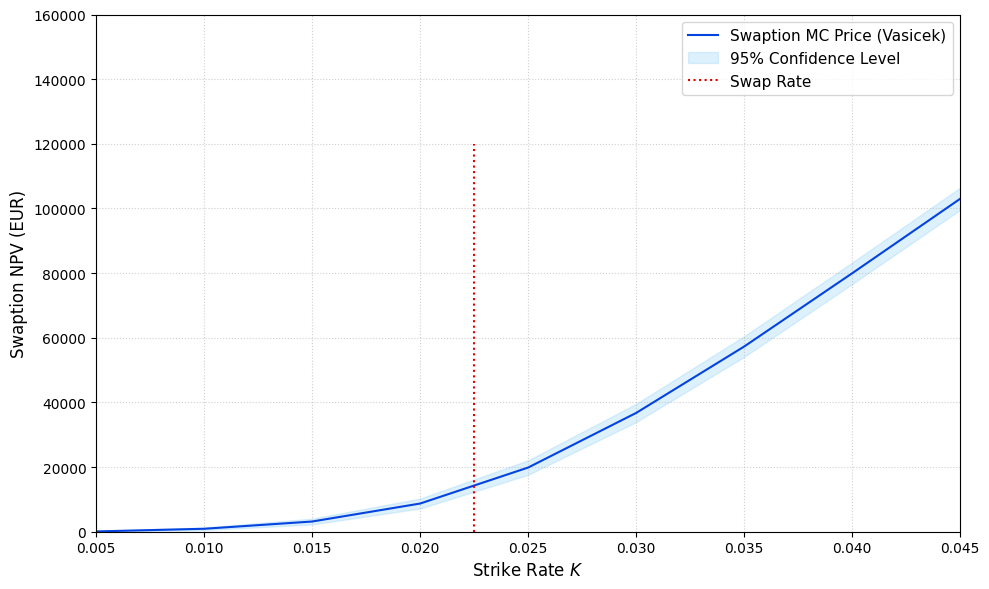
\includegraphics[width=0.6\textwidth]{figures/swaption_npv_vs_K}
\caption{Swaption NPV as a function of the strike $K$.}
\label{fig:swaption_npv_vs_K}
\end{figure}

\section*{Exercises}
\begin{question}
Assume that company A has agreed to pay a 6-month LIBOR and receive a fixed interest rate of 5.6\% per year (with interest payable every six months) from the face value of 100 million EUR. Swap is 1.5 years to expire. The interest rates for 6, 12 and 18 months are: 10\%, 10.5\% and 11\% respectively. Assume that interest rates are continuously compounded. The 6-month LIBOR is currently 10.2\%. 

Calculate the value of this swap for company A.
\end{question}

\cprotEnv\begin{solution}
\begin{ipython}
import pandas as pd
from finmarkets import InterestRateSwap, ForwardRateCurve, DiscountCurve
from datetime import date
from dateutil.relativedelta import relativedelta

fixed_rate = 0.056
tenor_fix = "6m"
tenor_float = "6m"
N = 100e6
obs_date = date.today()
start_date = obs_date 
discount_data = pd.read_excel('discount_curve.xlsx')
dates = [obs_date + relativedelta(months=i) for i in discount_data['months']]
dc = DiscountCurve(obs_date, dates, discount_data.loc[:, 'dfs'])

dates = [obs_date + relativedelta(months=i) for i in [0, 6, 12, 18]]
fr = ForwardRateCurve(obs_date, dates, [0.102, 0.10, 0.105, 0.11])

irs = InterestRateSwap(N, start_date, "18m", fixed_rate, tenor_float, tenor_fix)
print (f"IRS NPV: {-irs.npv(dc, fr):.2f} EUR")
\end{ipython}
\begin{ioutput}
IRS NPV: 84577.81 EUR
\end{ioutput}
\end{solution}

\begin{question}
Suppose that the IBOR forward rates and the discount curve are those defined in
\href{https://github.com/matteosan1/finance_course/raw/master/input_files/euribor_curve.xlsx}{euribor\_curve.xlsx} and \href{https://github.com/matteosan1/finance_course/raw/master/input_files/discount_curve.xlsx}{discount\_curve.xlsx} respectively.
Determine the value of an option to pay a fixed rate of 4\% and receives IBOR on a 5 year swap starting in 1 year. Assume the notional is 100 EUR, the exercise date is in one year from now and the swap rate volatility is 15\%.
\end{question}

\cprotEnv\begin{solution}
\begin{ipython}
import pandas as pd
from finmarkets import InterestRateSwaption, ForwardRateCurve, DiscountCurve
from datetime import date
from dateutil.relativedelta import relativedelta

obs_date = date.today()
start_date = obs_date + relativedelta(years=1)
exercise_date = start_date
discount_data = pd.read_excel('discount_curve.xlsx')
euribor_data = pd.read_excel('euribor_curve.xlsx')


dates = [obs_date + relativedelta(months=i) for i in discount_data['months']]
dc = DiscountCurve(obs_date, dates, discount_data.loc[:, 'dfs'])

dates = [obs_date + relativedelta(months=i) for i in euribor_data['months']]
fr = ForwardRateCurve(obs_date, dates, euribor_data['rates'])

sigma = 0.15
rate = 0.04
swaption = InterestRateSwaption(1e6, start_date, exercise_date,
                                "5y", sigma, rate, "6m")
print(f"Swaption NPV: {swaption.payoffBS(obs_date, dc, fr):.0f} EUR")
\end{ipython}
\begin{ioutput}
Swaption NPV: 16496600 EUR
\end{ioutput}
\end{solution}

%\begin{question}
%A \emph{currency swap}, sometimes referred to as a cross-currency swap, involves the exchange of interest—and sometimes of principal—in one currency for the same in another currency. Interest payments are exchanged at fixed dates through the life of the contract. 
%
%Assume that yield curves in Japan and in the US are flat. The interest rate in Japan is equal to 4\% per annum, and in the US to 9\% per annum (with continuous compounding). A financial institution takes position in a swap contract, under which it receives 5\% on an annual basis of the amount denominated in yen and pays 8\% per annum of the amount denominated in dollars. These amounts are respectively 10 million USD and 1200 million yen. The contract is valid for 3 years and the current exchange rate is 110 USDJPY. What is the value of this currency swap?
%
%\textbf{Hint:} write a \texttt{CurrencySwap} class in order to valuate the swap.
%\end{question}
%
%\cprotEnv\begin{solution}
%\begin{ipython}
%import numpy as np
%
%class CurrencySwap:
%    def __init__(self, amount_for, amount_dom, r_for, r_dom,
%                 fixed_for, fixed_dom, exchg_rate, maturity):
%        self.amount_for = amount_for
%        self.amount_dom = amount_dom
%        self.r_for = r_for
%        self.r_dom = r_dom
%        self.fixed_for = fixed_for
%        self.fixed_dom = fixed_dom
%        self.exchg_rate = exchg_rate # for/dom
%        self.maturity = maturity
%
%    def foreign_npv(self):
%        b_f = 0
%        for t in range(1, maturity+1):
%            b_f += np.exp(-self.r_for*t)*self.fixed_for*self.amount_for
%        b_f += np.exp(-self.r_for*t)*self.amount_for
%        return b_f
%
%    def domestic_npv(self):
%        b_d = 0
%        for t in range(1, maturity+1):
%            b_d += np.exp(-self.r_dom*t)*self.fixed_dom*self.amount_dom
%        b_d += np.exp(-self.r_dom*t)*self.amount_dom
%        return b_d
%
%    def value_dom(self):
%        return self.foreign_npv()/self.exchg_rate - self.domestic_npv()
%
%    def value_for(self):
%        return self.domestic_npv()*self.exchg_rate - self.foreign_npv() 
%\end{ipython}
%\noindent
%\begin{ipython}
%rf = 0.04
%rd = 0.09
%kf = 0.05
%kd = 0.08
%Nf = 1200e6
%Nd = 10e6
%S = 110
%
%cs = CurrencySwap(Nf, Nd, rf, rd, kf, kd, S)
%print ("Domestic Value: {:.0f} USD".format(cs.value_dom()))
%print ("Foreign Value: {:.0f} yen".format(cs.value_for()))
%\end{ipython}
%\begin{ioutput}
%Domestic Value: 1542996 USD
%Foreign Value: -169729535 yen
%\end{ioutput}
%
%The swap value for the financial institution is about 1.54 million USD. If the institution paid in yen and received cash flows in dollars, the swap value would be around -1697 million yen.
%\end{solution}
 
\chapter{Optimizing Monte Carlo}
\label{cap:variation_reduction}

Results of Monte Carlo simulations are always estimates with a margin of error. \emph{Variance Reduction Techniques} (VRTs) are a set of
mathematical strategies designed to make that estimate more precise (reducing the "noise" or variance) without requiring millions of additional, computationally expensive simulations.
	
Think of it like trying to determine the average height of people in a city. You could either: pick 100 people completely at random (standard method), or pick 50 people at random, 
but for every tall person you pick, you intentionally pick a short person to balance the scale (VRT method). The second approach reaches the "true" average much faster because
you've manually removed the extreme outliers that skew the results.
	
When you simulate a complex model like Vasicek or GBM, "raw" Monte Carlo is often too slow or jittery for real-time risk management. VRTs  allow you to achieve the same level of accuracy with smaller effort.

Some of the most popular variation reduction techniques will be described in this Chapter:
	
\begin{itemize}
	\tightlist
	\item Antithetic Variates
	\item Control Variates
	\item Importance Sampling
\end{itemize}
	
As we have seen the standard error of a Monte Carlo estimate is given by: $\text{standard error} = \frac{\sigma}{\sqrt{N}}$. To cut the error in half using the standard method, you need 4 times
more paths ($N$). With Variance Reduction, instead of increasing $N$, you focus on shrinking $\sigma$ (the numerator) through clever sampling, which is often much more efficient for high-performance
banking systems.
	
\section{Antithetic Variates}
\label{sec:monte-carlo-with-antithetic-variates}
	
\emph{Antithetic Variates} is a powerful \textbf{variance reduction} technique used in Monte Carlo simulations to improve computational efficiency and precision. The core idea is to introduce a deliberate
negative correlation between pairs of simulated paths. 

For every random sample $Z$ drawn from a standard normal distribution to generate a path, a second "mirror" path is generated using $-Z$. By averaging these two complementary observations, the terms with high
positive variance tend to cancel out those with high negative variance. Mathematically, this reduces the standard error of the estimate because the covariance between the two paths is negative, leading to a faster
convergence toward the true value compared to using twice as many independent random draws.
	
Technically, the Antithetic Variates technique can be used for any distribution, but it is most effective and straightforward when the distribution is symmetric around a mean.
	
While the \emph{normal distribution} is the most common use case (especially in finance), the principle relies on the probability integral transform, see Sec.~\ref{sec:distribution-transformation}.

\paragraph{Symmetric Distributions}: if a distribution is symmetric around its mean $\mu$, you can generate antithetic paths directly. If you sample $X$, your antithetic sample is $X'=2\mu -X$ 
(in the case of a Standard Normal $\mathcal{N}(0,1)$, this simplifies to $X'=-X$).

\paragraph{Non-Symmetric Distributions}: even if a distribution is not symmetric, you can still use the technique. This is because almost all random variables are generated by transforming a Uniform distribution $\mathcal{U}(0,1)$. The "mirroring" happens at the Uniform level: generate a random number $u$ from $\mathcal{U}(0,1)$, use $1-u$ as your antithetic sample, transform both ($u$ and $1-u$) into your target
distribution using the Inverse Cumulative Distribution Function ($F^{-1}$).

As an example let's see how to simulate an exponential distribution. Its CDF is: $F(x)=1-e^{-\lambda x}$. To sample, we set $F(x)=u$ (where $u$) is a random uniform number
between 0 and 1). Solving for x: 
\begin{equation}
	\begin{gathered}
		u=1-e^{-\lambda x} \\
		1-u=e^{-\lambda x} \\
		\ln(1-u)=-\lambda x \\
		x=-\ln(1-u)/\lambda
	\end{gathered}
\end{equation}

Finally you take $X=\frac{-\ln(u)}{\lambda}$ and $X'=\frac{-\ln(1-u)}{\lambda}$. These two values will be negatively correlated, successfully reducing variance.
	
The effectiveness of Antithetic Variates depends on the function you are simulating being monotonic. If the function is not or if the variance of the average of the pairs is higher than the variance of the individual
samples, the technique fails. The mathematical condition for success can be expressed as 

\begin{equation}
\var(f(U))+\var (f(1-U))+2\cov (f(U),f(1-U))]
\end{equation}
	
This occurs only if $\cov(f(U),f(1-U))<0$ (negative correlation). In the $x^2$ example: Since $(x)^2=(-x)^2$, the correlation is +1, which actually maximizes the estimate variance instead of reducing it.
	
This example shows the use of antithetic variates for estimating the mean and standard error of two different functions: $X^2$ and $e^{X/2}$, where $X$ follows a standard normal distribution.

\begin{ipythonnon}
import numpy as np
import matplotlib.pyplot as plt

def simulate_exp2(n_samples):
	x1 = np.random.randn(n_samples)
	x2 = -x1
	x_std = np.random.randn(n_samples*2)
	return np.exp(x1/2), np.exp(x2/2), np.exp(x_std/2)

def simulate_x2(n_samples):
	x1 = np.random.randn(n_samples)
	x2 = -x1
	x_std = np.random.randn(n_samples*2)
	return np.power(x1, 2), np.power(x2, 2), np.power(x_std, 2)

def simulate_exponential(n_samples, rate=1.0):
	u = np.random.uniform(0, 1, n_samples // 2)
	u_antithetic = 1 - u
	x1 = -np.log(u) / rate
	x2 = -np.log(u_antithetic) / rate
	x_std = -np.log(np.random.uniform(0, 1, n_samples)) / rate    
	return x1, x2, x_std

def analysis(x1, x2, x_std):
	anti_mean = (x1 + x2) / 2
	std_mean = x_std.reshape(-1, 2).mean(axis=1)
	
	print(f"Variance (Standard MC): {np.var(std_mean):.6f}")
	print(f"Variance (Antithetic):  {np.var(anti_mean):.6f}")
	print(f"Reduction: {100*(1-np.var(anti_mean)/np.var(std_mean)):.2f}%")

N = 20000
x1, x2, x_std = simulate_exponential(N)
analysis(x1, x2, x_std)	

x1, x2, x_std = simulate_x2(N)
analysis(x1, x2, x_std)

x1, x2, x_std = simulate_exp2(N)
analysis(x1, x2, x_std)
\end{ipythonnon}
\begin{ioutput}
Variance (Standard MC): 0.181873
Variance (Antithetic):  0.038561
Reduction: 78.80%
Variance (Standard MC): 1.012585
Variance (Antithetic):  2.014346
Reduction: -98.93%
Variance (Standard MC): 0.506297
Variance (Antithetic):  0.183833
Reduction: 63.69%
\end{ioutput}
	
\subsection{European Call Option with Antithetic Variates}
\label{sec:monte-carlo-european-call-option-with-antithetic-variates}
	
Here we implement a Monte Carlo simulation to price a European call option, incorporating the antithetic variates technique for variance reduction.
	
\begin{ipythonnon}
import numpy as np
from scipy.stats import norm

def mc_comparison(S0, K, r, T, sigma, n):
	A = (r - 0.5 * sigma**2) * T
	B = sigma * np.sqrt(T)
	discount = np.exp(-r * T)
	
	Z = np.random.randn(n)
	payoff_a1 = np.maximum(0, S0 * np.exp(A + B * Z) - K)
	payoff_a2 = np.maximum(0, S0 * np.exp(A + B * (-Z)) - K)
	
	E_antithetic = discount * 0.5 * (payoff_a1 + payoff_a2)
	price_anti = np.mean(E_antithetic)
	se_anti = np.std(E_antithetic) / np.sqrt(n)
	
	Z_std = np.random.randn(2 * n)
	payoff_std = discount * np.maximum(0, S0 * np.exp(A + B * Z_std) - K)
	
	price_std = np.mean(payoff_std)
	se_std = np.std(payoff_std) / np.sqrt(2 * n)
	
	return (price_anti, se_anti), (price_std, se_std)

S0, K, r, T, sigma, n = 100, 100, 0.05, 1, 0.2, 10000

(p_anti, s_anti), (p_std, s_std) = mc_comparison(S0, K, r, T, sigma, n)

print(f"Antithetic: Price = {p_anti:.4f}, Std Error = {s_anti:.6f}")
print(f"Standard:   Price = {p_std:.4f}, Std Error = {s_std:.6f}")
print(f"Variance Reduction: {100*(1-(s_anti**2/s_std**2)):.2f}%")
\end{ipythonnon}	
	
\begin{ioutput}
Antithetic: Price = 10.6164, Std Error = 0.074618
Standard:   Price = 10.5487, Std Error = 0.104660
Variance Reduction: 49.17%
\end{ioutput}
	
Try to guess what would be the outcome of a similar simulation involving a \emph{Straddle} option (a bet on volatility), whose payoff $V$ is $|S_T - K|$.
	
\section{Control Variates}

Control Variates is a variance reduction technique that improves the precision of a Monte Carlo simulation by leveraging the known solution of a simpler, related problem.

In this approach, instead of simulating only the target asset (the "unknown"), you simultaneously simulate a "control" variable whose expected value is already known analytically. 
By observing how the simulated control variable deviates from its true theoretical value, you can apply a correction to the target simulation.

For instance, when pricing a complex Asian option, a practitioner might use a standard European option as the control variate. If the European simulation happens to overestimate the 
price due to random noise, the Asian estimate is adjusted downward by a proportional amount. This "error correction" significantly narrows the confidence intervals, allowing for 
high-precision results with far fewer paths.

Mathematically, the Control Variates technique is rooted in the property of the variance of a sum. When you add a "control" to your estimator, you are effectively performing a linear regression on the noise.
Here is the step-by-step mathematical breakdown. 

Suppose we want to estimate $\mu =\mathbb{E}[Y]$ (e.g., the expected payoff of a complex option). We find another variable $X$ (the control) where we already know the true expected value
$\mu_X=\mathbb{E}[X]$ analytically. We define a new estimator, $Y_{CV}$: 
\begin{equation}
Y_{CV}=Y+c(X-\mathbb{E}[X])
\end{equation}

Notice that $Y_{CV}$ is an unbiased estimator because if you take the expectation of both sides: 
\begin{equation}
\mathbb{E}[Y_{CV}]=\mathbb{E}[Y]+c(\mathbb{E}[X]-\mathbb{E}[X])=\mathbb{E}[Y]
\end{equation}

The goal is to choose a constant $c$ that makes $\var(Y_{CV})$ as small as possible. The variance of our new estimator is:
\begin{equation}
\var(Y_{CV})=\var(Y+cX)=\var(Y)+\var(X)+2c\cov(Y,X)
\end{equation}

To find the minimum, we take the derivative with respect to $c$ and set it to zero: 
\begin{equation}
\frac{d\var(Y_{CV})}{dc} = 2c\var(X)+2\cov(Y,X)=0
\end{equation}

Solving for $c$: 
\begin{equation}
c^*= -\frac{\cov(Y,X)}{\var(X)}
\end{equation}

If we plug this optimal $c^*$ back into the variance equation, we get the minimum variance: 
\begin{equation}
\var(Y_{CV})=\var(Y)-\frac{\cov(Y,X)^2}{\var(X)}=\var(Y)(1-\rho_{XY}^2)
\end{equation}
where $\rho_{XY}$ is the correlation coefficient between your target $Y$ and your control $X$. If $\rho =1$ (perfect correlation), the variance becomes zero. If $\rho =0$ (no correlation), the variance
remains $\var(Y)$. Even a moderate correlation (e.g., 0.9) results in a $1-0.92=19\%$ residual variance, meaning an 81\% reduction.
	
\subsection{European Call Option with Control Variates}
\label{sec:monte-carlo-european-call-option-with-control-variates}
	
Here we will see a Monte Carlo simulation to price a European call option using the control variates technique for variance reduction.
	
\begin{ipythonnon}	
import numpy as np

def mc_control_variate(S0, K, r, T, sigma, n):
	dt = T
	drift = (r - 0.5 * sigma**2) * dt
	vol = sigma * np.sqrt(dt)
	discount = np.exp(-r * T)
	
	Z = np.random.randn(n)
	ST = S0 * np.exp(drift + vol * Z)
	
	Y = discount * np.maximum(0, ST - K)
	
	X = discount * ST
	E_X = S0 
	
	cov_matrix = np.cov(Y, X)
	c = -cov_matrix[0, 1] / cov_matrix[1, 1]
	
	Y_cv = Y + c * (X - E_X)
	
	price_cv = np.mean(Y_cv)
	se_cv = np.std(Y_cv) / np.sqrt(n)
	
	price_std = np.mean(Y)
	se_std = np.std(Y) / np.sqrt(n)
	
	return (price_cv, se_cv), (price_std, se_std)

S0, K, r, T, sigma, n = 100, 105, 0.05, 1, 0.2, 20000

(p_cv, s_cv), (p_std, s_std) = mc_control_variate(S0, K, r, T, sigma, n)

print(f"Standard MC: {p_std:.4f} (SE: {s_std:.6f})")
print(f"Control Var: {p_cv:.4f} (SE: {s_cv:.6f})")
print(f"Variance Reduction: {100*(1-(s_cv**2/s_std**2)):.2f}%")	
\end{ipythonnon}
\begin{ioutput}
Standard MC: 8.0789 (SE: 0.093061)
Control Var: 7.9719 (SE: 0.042260)
Variance Reduction: 79.38%
\end{ioutput}
	
\section{Importance Sampling}
\label{sec:importance-sampling}

Assume we want to calculate the expectation $\mathbb{E}[f(X)] = \int_{-\infty}^\infty f(x)p(x)dx$ where $p(x)$ is the probability density function associated to $X$.

We can approximate this expectation using numerical approximation by sampling $n$ random values from the distribution $p$ and then calculate the sample mean:
\begin{equation}
\bar{f}(x) = \frac{1}{n}\sum_i f(x_i)
\end{equation}

The idea behind \textbf{importance sampling} is to use a simple re-formulation trick and write the expectation as
\begin{equation}
\mathbb{E}[f(X)] = \int_{-\infty}^\infty f(x)\frac{p(x)}{q(x)}q(x)dx
\end{equation}
giving the expectation of $f(x)p(x)/q(x)$ over the distribution $q$. And with that, allowing us to calculate the sample mean by sampling from $q$:
\begin{equation}
\bar{f}(x) = \frac{1}{n}\sum_i f(x_i)\frac{p(x)}{q(x)}
\end{equation}

\section{Variance Reduction}
\label{variance-reduction}

The variance of the standard Monte Carlo estimator is given by:
\begin{equation}
\frac{1}{n}\var[f(x)] = \frac{1}{n}\mathbb{E}[(f(X)-\mathbb{E}[f(X)])^2]
\end{equation}

The variance for the reformulated importance sampling estimator is:
\begin{equation}
\frac{1}{n}\var\left[\frac{p(x)}{q(x)}f(x)\right]
\end{equation}

This give us a hint on how to find a way to reduce the variance. And indeed it is relatively easy to see that this variance could be reduced to 0 by choosing $q$ as:
\begin{equation}
	\begin{split}
		q(x) = \frac{f(X)p(x)}{\mathbb{E}[f(X)]} &\implies \frac{1}{n}\var[\mathbb{E}[f(X)]] = \frac{1}{n}\mathbb{E}[(\mathbb{E}[f(X)]-\mathbb{E}[\mathbb{E}[f(X)]])^2] \\
		&= \frac{1}{n}\mathbb{E}[(\mathbb{E}[f(X)]-\mathbb{E}[f(X)])^2] = 0
	\end{split}
\end{equation}

Naturally, we don't know $\mathbb{E}[f(X)]$, as the reason we are doing this sampling after all is to find the expectation of $f$.

However, we can think of the denominator of the previous expression as some normalisation constant, and consider to construct $q$ such that it has \textbf{high} density wherever $f(x)p(x)$ is \textbf{high}.

\subsubsection{A Practical Example}

For the sake of demonstration, we choose $f=\mathcal{N}(5, 1)$, and the probability distribution $p=\mathcal{N}(9,2)$ which do not overlap too well, see Fig.~\ref{fig:importance_sampling_1}.
\begin{ipythonnon}
import numpy as np
import matplotlib.pyplot as plt

from scipy.stats import norm

f = norm(5, 1)
p = norm(9, 2)
\end{ipythonnon}

\begin{figure}[htb]
	\centering
	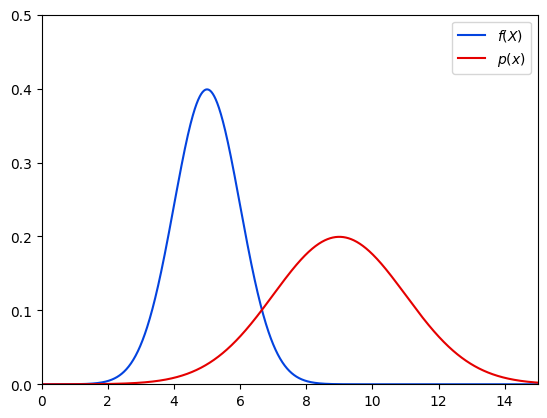
\includegraphics[width=0.7\textwidth]{figures/importance_sampling_1}
	\caption{$f$ and $p$ distributions used in the example.}
	\label{fig:importance_sampling_1}
\end{figure}

To approximate numerically the expectation, as stated above, we would now sample values $x_i$ from the distribution $p$, and compute the mean of $f(x_i)$.

Intuitively one can see why sampling from this distribution is a bad idea: for most values sampled from $p$, $f$ will be close to 0, but for a few sampled values $f$ will be very large, thus we obtain a
large variance.
\begin{ipythonnon}
N = 10000
samples = p.rvs(size=N)
f_sampling = f.pdf(samples)
mean = f_sampling.mean()
variance = f_sampling.var()

print (f"Numerical Simulation: mean {mean:.5f}, variance {variance:.5f}")
\end{ipythonnon}
\begin{ioutput}
Numerical Simulation: mean 0.03578, variance 0.00767
\end{ioutput}

Figure~\ref{fig:importance_sampling_2} (left) shows the distribution of the simulation results, there is a huge peak at 0, while the non-zero events are spread up to 0.4 leading to a large variance.

Therefore, as outlined above, we now try a new distribution $q = \mathcal{N}(5.8, 1)$, which satisfies the criterion that its PDF is high in regions where $f(x)p(x)$ is high.

\begin{figure}[htb]
	\centering
	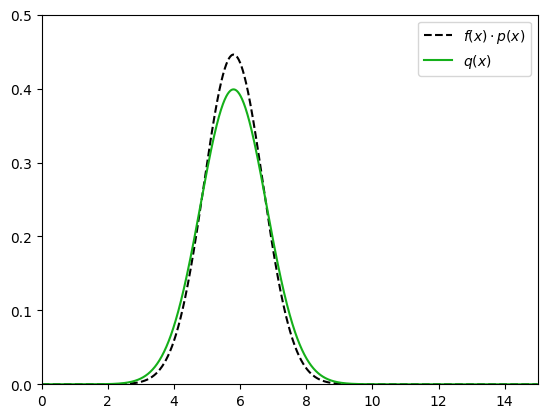
\includegraphics[width=0.7\textwidth]{figures/importance_sampling_3}
	\caption{Distribution of function $q$ to be used in the importance sampling example. Notice how it is non-zero in the relevant region $f(x)p(x) \gg 0$.}
	\label{fig:importance_sampling_3}
\end{figure}

\begin{ipythonnon}
samples2 = q.rvs(size=N)
f_sampling2 = f.pdf(samples2)*p.pdf(samples2)/q.pdf(samples2)
mean2 = f_sampling2.mean()
variance2 = f_sampling2.var()

print (f"Numerical Simulation: mean {mean:.5f}, variance {variance:.5f}")
print (f"Importance Sampling: mean {mean2:.5f}, variance {variance2:.5f}")
\end{ipythonnon}
\begin{ioutput}
Numerical Simulation: mean 0.03581, variance 0.00760
Importance Sampling: mean 0.03602, variance 0.00003
\end{ioutput}

Figure~\ref{fig:importance_sampling_2} (right) shows the distribution of the the simulation results, now the data is much more condensed around the mean leading to a much lower variance.
Looking at the numerical results we achieved a reduced variance by a factor of 200,  still with the correct mean (and the same number of samples).

\begin{figure}[htb]
	\centering
	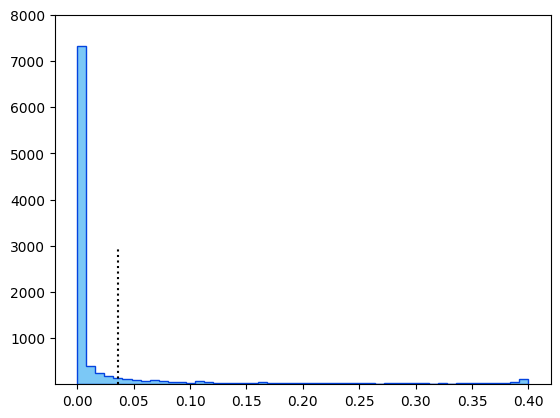
\includegraphics[width=0.45\textwidth]{figures/importance_sampling_2}
	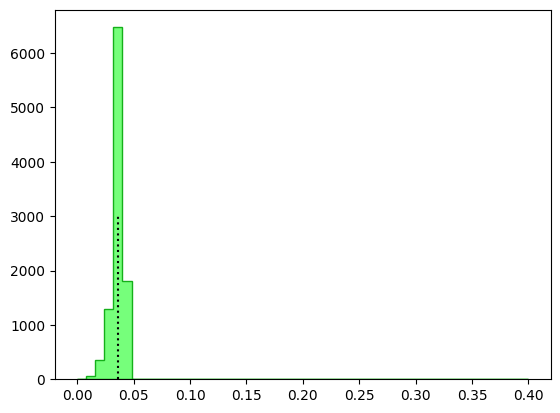
\includegraphics[width=0.45\textwidth]{figures/importance_sampling_4}
	\caption{The distribution of simulated results with standard Monte Carlo (left) and with importance sampling Monte Carlo (right). The dashed line represents the mean.}
	\label{fig:importance_sampling_2}
\end{figure}

\textbf{Note} it's not trivial to find $q$, and certainly there are much more difficult real-word scenarios. For this example I actually plotted $p(x)f(x)$ and then picked a $q$ which resembled it best.

\subsubsection{How unlucky is a 25 standard deviation return ?}
\label{sec:how-unlucky-is-a-25-standard-deviation-return}

Imagine you want to estimate the following probability:
\begin{equation}	
\theta := P(X\geq 25) = \mathbb{E}[\mathbbm{1}_{X\geq 25}]  \quad\text{where } X\sim \mathcal{N}(0, 1)
\end{equation}

The standard Monte Carlo approach proceeds as follows: generate $(X_1, X_2, \ldots ,X_n$ i.i.d. $\mathcal{N}(0,1)$; set $\mathbbm{1}_j=\mathbbm{1}_{X_j\geq 25}$ for $j=1,\ldots ,n$, set
$\hat{\theta}=\sum_{j=1}^n \mathbbm{1}_j/n$, compute approximate 95\% c.l. as $\hat{\theta}_n\pm 1.96\hat{\sigma}_n/\sqrt{n}$.

Why is this a bad idea ? Beyond knowing that $\theta$ is very small, do we even care about estimating $\theta$ accurately ?

\begin{ipythonnon}
import numpy as np
M = 1000000
Z = np.random.normal(size=M)

# Indicator function, count number of sampled variables above 25
ZT = np.where(Z>25, 1, 0)
X = np.mean(ZT)

# Calculate standard error and 95% Condifence intervals
sigma = np.std(ZT)
SE = sigma/np.sqrt(M)
CIs = [X-SE*1.96, X+SE*1.96]

print (X)
print(f'95% Confidence Level. Returns are [{CIs[0]:0.3e}, {CIs[1]:0.3e}]')
\end{ipythonnon}
\begin{ioutput}
0.0
95\% Confidence Levels. Returns are [0.000e+00, 0.000e+00]
\end{ioutput}

We have got 0 because not even one "simulation" returned a value larger than 25. So it would be better to say that the result is \textbf{undefined}.
Starting today and simulating 1 million experiments per second, most likely our Sun will be dead well before we have got a non-zero result from our MC.

Using the importance sampling technique instead we can improve our estimate giving a meaningful result.

Let's write 
\begin{equation}
	\begin{aligned}
		\theta &= \mathbb{E}[\mathbbm{1}_{\{X\geq 25\}}] = \int_{-\infty}^{\infty}\mathbbm{1}_{\{X\geq 25\}}\cfrac{1}{\sqrt{2\pi}}\exp{\left(-\frac{x^2}{2}\right)}dx = \\
		&= \int_{-\infty}^{\infty}\mathbbm{1}_{\{X\geq 25\}} \left(
		\cfrac{\frac{1}{\sqrt{2\pi}}\exp{\left(-\frac{x^2}{2}\right)}}{\frac{1}{\sqrt{2\pi}}\exp{\left(-\frac{(x-\color{red}{\mu})^2}{2}\right)}}
		\right) \frac{1}{\sqrt{2\pi}}\exp{\left(-\frac{(x-\color{red}{\mu})^2}{2}\right)}dx =\\
		&= \mathbb{E}_\mu\left[\mathbbm{1}_{\{X\geq 25\}} \cfrac{1}{\sqrt{2\pi}}\exp{\left(-\frac{-\color{red}\mu X+\color{red}\mu^2}{2}\right)} \right]
	\end{aligned}
\end{equation}

Now choosing $X\sim\mathcal{N}(\mu, 1)$ with $\mu=25$ leads to a much more efficient estimator as can be seen from the following simulation (\textbf{note how 1000 events are now enough to get a
meaningful result}).

\begin{ipythonnon}
from scipy.stats import norm

M = 1000
mu = 25

np.random.seed(1)

# Method 1 - use scipy stats PDF functions
p = norm(0, 1)
q = norm(mu, 1)
x = q.rvs(size=M)
ZT = np.where(x>25, 1, 0) * p.pdf(x)/q.pdf(x)

# Method 2 - direct with analytical ratio
#ZT = np.where(x>25,1,0)*np.exp(-mu*x + mu**2/2)

X = np.mean(ZT)
sigma = np.std(ZT)
SE = sigma/np.sqrt(M)
CIs = [X-SE*1.96,X+SE*1.96]
print (X)
print(f'95% Confidence Levels are [{CIs[0]:0.3e}, {CIs[1]:0.3e}]')
\end{ipythonnon}
\begin{ioutput}
2.810646171611043e-138
95\% Confidence Levels are [1.873e-138, 3.748e-138]
\end{ioutput}

\subsection{European Call Option with Importance Sampling}
\label{sec:monte-carlo-european-call-option-with-importance-sampling}
	
Suppose we wish to estimate the value of a call option which is well "out of the money" using Monte Carlo methods ($K \gg S_0$).

In this case, using crude Monte Carlo, the majority of the values randomly generated for $S_T$ would fall below the strike and contribute zero to the option price.

One possible remedy is to generate values of $S_T$ under a distribution that is more likely to exceed the strike, but of course this would increase the simulated value of the option. So we need to
compensate for changing the underlying distribution by multiplying by a factor adjusting the mean (i.e.~importance sampling).

More specifically, we wish to estimate
\begin{equation}
\mathbb{E}^{\mathbb{Q}}[e^{-rT}(S_0e^{Z_t}-K)^+],\text{ where }Z_t\sim\mathcal{N}((r-\sigma^2/2)T,\sigma^2T)
\end{equation}

Suppose we modify the underlying probability measure of $Z_T$ to $\mathbb{Q}_0$ with a larger drift.

The new simulation generates paths that are less likely to produce options expiring with zero value, and in a sense has this eliminated some computational waste.
\begin{ipythonnon}
import numpy as np

from finmarkets import GBM
from finmarkets.options.vanilla import call

S0 = 100.0
K = 170.0
T = 1.0
mu = 0.06
vol = 0.20
N = 100
tsteps = 100

np.random.seed(1)
ST = GBM(mu, vol, S0, T, tsteps, N)
ST2 = GBM(0.5, vol, S0, T, tsteps, N)

C_BS = call(S0, K, mu, vol, 1)
print (f"{C_BS:.4f}")
\end{ipythonnon}
\begin{ioutput}
0.0789
\end{ioutput}

\begin{figure}[htb]
	\centering
	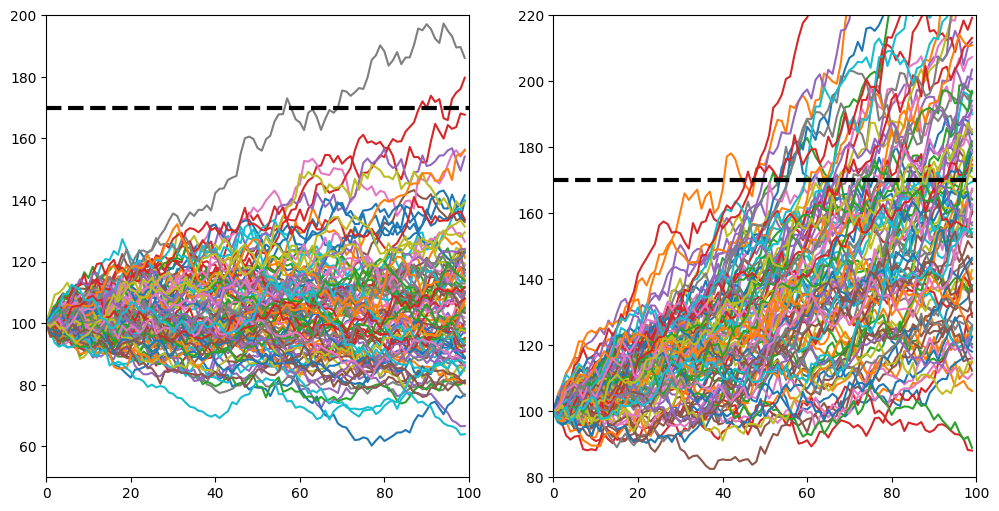
\includegraphics[width=0.85\textwidth]{figures/importance_sampling_5}
	\caption{Distribution of GBM paths (left) with real drift term, (right) with adjusted drift term.}
	\label{fig:importance_sampling_5}
\end{figure}

There is a clear connection between importance sampling and Radon-Nikodym derivative (or Girsanov theorem):
\begin{equation}
	\begin{gathered}
		\mathbb{E}[f(x)] = \int f(x)p(x) dx = \int f(x) \cfrac{p(x)}{q(x)} dx\\
		\mathbb{E}^{\mathbb{Q}}[f(S_T)]= \mathbb{E}^{\mathbb{Q}_0}\left[f(S_T)\cfrac{d\mathbb{Q}}{d\mathbb{Q}_0}\right]
	\end{gathered}
\end{equation}

The importance sampling adjustment that insures that the estimator continues to be an unbiased estimator of the option price is the ratio of the two probability densities (likelihood ratio).
So we can simulate events under $\mathbb{Q}_0$ and the multiply by the Radon-Nikodym derivative. So we get
\begin{equation}
	\begin{gathered}
		\mathbb{E}^{\mathbb{Q}}[e^{-rT}(S_0 e^{Z_T} - K)^+], \text{ where } Z_T\sim \mathcal{N}((r-\cfrac{\sigma^2}{2})T, \sigma^2T) \\
		\mathbb{E}^{\mathbb{Q}_0}[e^{-rT}(S_0 e^{Z_T} - K)^+], \text{ where } Z_T\sim \mathcal{N}(\mu T, \sigma^2T)
	\end{gathered}
\end{equation}

We would like to determine the \emph{optimal} $\mu$ such that the variance is minimized. Unfortunately there is not straightforward way to do that. One can try to determine a relatively optimal value by
\begin{equation}
\min_{\mu}\mathbb{E}^{\mathbb{Q}}\left[f^2(x)\cfrac{p(x)}{q_\mu(x)}\right]
\end{equation}

\begin{ipythonnon}
from scipy.stats import norm
from scipy.optimize import fmin, minimize

def Q0(mu, x, sigma, T):
	return norm(mu*T, sigma*T).pdf(x)

def Q(x, r, sigma, T):
	return norm((r - 0.5*sigma**2)*T, sigma*T).pdf(x)

def f(x, r, S0, K):
	return np.exp(-r*T)*np.maximum(0, S0*np.exp(x) - K)

M = 1000000
def arg_min(x, mu, sigma, T):
	x_T = np.random.normal(size=M)
	z = (mu - 0.5*sigma**2)*T + sigma*x_T*np.sqrt(T)
	return np.mean(f(z, mu, S0, K)**2*Q(z, mu, vol, T)/Q0(x, z, vol, T))

res = minimize(arg_min, 0.6, args=(mu, vol, T), method='Nelder-Mead',
               options={'maxiter':2000})
print (res)
mu_star = res.x	
\end{ipythonnon}
\begin{ioutput}
message: Optimization terminated successfully.
success: True
status: 0
fun: 0.012807191452145612
x: [ 6.295e-01]
nit: 10
nfev: 26
final_simplex: (array([[ 6.295e-01], [6.296e-01]]), 
                array([ 1.281e-02,  1.287e-02]))
\end{ioutput}

So we can check how importance sampling works with different number of samples. ranging from 100 to 50000, see Fig.~\ref{fig:importance_sampling_6}.

\begin{ipythonnon}
np.random.seed(1)
C0_is, SE_is = [], []
C0_wo, SE_wo = [], []

Ms = [100, 500, 1000, 2500, 5000, 10000, 25000, 50000]
for M in Ms:
	x_T = np.random.normal(size=M)
	z = mu_star*T - vol*x_T*np.sqrt(T)
	C_is = f(z, mu, S0, K)*Q(z, mu, vol, T)/Q0(mu_star, z, vol, T)

z = (mu-0.5*vol**2)*T + vol*x_T*np.sqrt(T)
C_wo = f(z, mu, S0, K)
C0_is.append(np.mean(C_is))
SE_is.append(np.std(C_is))
C0_wo.append(np.mean(C_wo))
SE_wo.append(np.std(C_wo))

data = pd.DataFrame({"M":Ms, "DP_wo":C0_wo, "DP_is":C0_is, "std_wo":SE_wo,
                     "std_is":SE_is})
data['reduction'] = data['std_wo']/data['std_is']
print (data.head(20))
\end{ipythonnon}
\begin{ioutput}
       M     DP_wo     DP_is    std_wo    std_is  reduction
0    100  0.000000  0.088340  0.000000  0.085636   0.000000
1    500  0.156567  0.074716  2.661602  0.082478  32.270467
2   1000  0.072207  0.080365  1.183912  0.085448  13.855288
3   2500  0.090879  0.078064  1.512354  0.083297  18.156072
4   5000  0.106882  0.079540  1.624668  0.084151  19.306581
5  10000  0.071713  0.078611  1.308213  0.083662  15.636928
6  25000  0.079021  0.078641  1.238422  0.083380  14.852823
7  50000  0.083900  0.078832  1.343988  0.083419  16.111264
\end{ioutput}

\begin{figure}[htb]
	\centering
	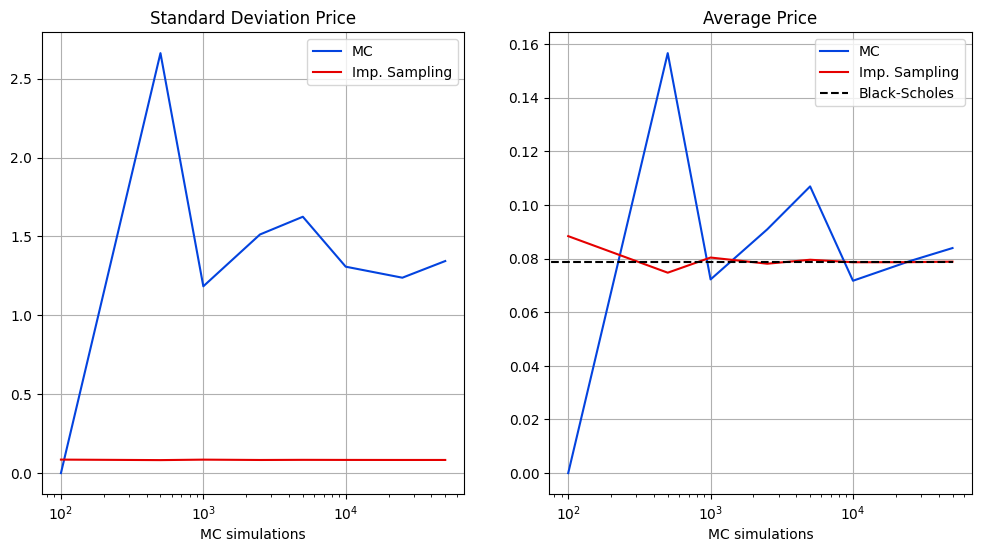
\includegraphics[width=0.8\textwidth]{figures/importance_sampling_6}
	\caption{Convergence of the importance sampling technique compared to "raw" Monte Carlo as a function of the number of simulations. It is apparent how the variation reduction technique dramatically improves
	the result.}
	\label{fig:importance_sampling_6}
\end{figure}

\subsection{Variation Reduction Techniques Comparison}
There is a common misconception that Importance Sampling (IS) is always the "strongest" technique. In reality, IS is a specialized tool, whereas Control Variates (CV) and Antithetic Variates
(AV) are general-purpose tools.

Indeed comparing the results of the previous examples turns out that IS is not the best method, this conclusion can be due to the following issue.
Importance Sampling is designed to solve one specific problem: \emph{rare events}.
Considering again the European option case we may have two possibilities. If $S_0=100$ and $K=100$, the option is at-the-money and it has a 50\% chance of finishing in the money. Standard MC is already very good here. If you use IS, you are "forcing" the math to look at something it already sees clearly, often adding noise via the likelihood ratio.
If instead $S_0=100$ but $K=180$ (deep out-of-the-money), the option only finishes in the money 1\% of the time. Standard MC will give you zeros for 99\% of paths (huge variance). This is where IS wins, 
because it forces the simulation to look at that 1\% area.

In IS, your estimator is: $\text{Payoff}\times \text{Likelihood Ratio}$; with the likelihood ratio being an exponential function. Exponential functions have very high variance so
\begin{itemize}
	\item In Antithetic, you are averaging two correlated payoffs. This smooths the data.
	\item  In Control Variates, you	are subtracting known error. This anchors the data.
	\item In Importance Sampling, you are multiplying the payoff by a volatile weight. If your shift ($\mu_{shift}$) is too aggressive, the weight can explode or vanish, increasing the intrinsic standard deviation of the samples.
\end{itemize} 

%%This section implements a Monte Carlo simulation to price a European call option using the importance sampling technique for variance reduction.
%%	
%%	\textbf{Note on the original MATLAB code:} The provided MATLAB code for
%%	importance sampling contained some issues in the calculation of the
%%	likelihood ratio (\texttt{is\_ratio}) and the final estimator.
%%	Specifically, \texttt{VY\ =\ A\_is\ +\ B*n;} incorrectly used \texttt{n}
%%	(number of paths) instead of a random variable, and the
%%	\texttt{is\_ratio} and final \texttt{E\_is} calculations did not follow
%%	the standard importance sampling methodology. The
%%	\texttt{normfit(DiscPayoff.*ISRatios)} also referred to undefined
%%	variables and an inappropriate function for simply getting the mean/std.
%%	
%%The Python code below implements a standard and correct importance sampling approach, where we shift the mean of the underlying normal distribution to focus sampling efforts on the region where the option
%%has a non-zero payoff (i.e., where \(S_T > K\)). We then adjust the	payoffs by the likelihood ratio (Radon-Nikodym derivative) to ensure the estimator remains unbiased.
%%	
%%Yes, this code is mathematically and logically correct for implementing	Importance Sampling (IS) in the Black-Scholes framework.
%%	
%%You have correctly applied the Change of Measure (Girsanov Theorem simplified for the normal distribution). By shifting the mean of Z, you are forcing the simulation to generate more ``In-The-Money'' (ITM)
%%paths, which are the ones that actually contribute to the option's value. Why the Math is Correct 1. The Shift (μshift\hspace{0pt})
%%	
%%You chose μshift\hspace{0pt} such that the ``average'' simulated price ST\hspace{0pt} ends up exactly at the strike K.
%%	
%%\begin{verbatim}
%%In standard Monte Carlo, if an option is Out-of-the-Money (OTM), most paths result in a payoff of 0. This is "wasted" computation.
%%		
%%By shifting the distribution, you ensure that roughly 50% of your paths end up ITM, providing more "information" to the estimator.
%%\end{verbatim}
%%	
%%	\begin{enumerate}
%%		\def\labelenumi{\arabic{enumi}.}
%%		\setcounter{enumi}{1}
%%		\tightlist
%%		\item
%%		The Likelihood Ratio (Radon-Nikodym Derivative)
%%	\end{enumerate}
%%	
%%When you change the distribution from P to Q, you must multiply the	result by the likelihood ratio L=dQdP\hspace{0pt} to keep the estimator unbiased. For a shift in a normal distribution N(0,1)→N(μ,1), the ratio
%%is: L(Z)=exp(−μZ+21\hspace{0pt}μ2)
%%	
%%(Note: Your code uses - 0.5 * mu\_shift**2, which is correct because you are evaluating it using the original samples Z before the shift was applied). 
%%In your code, you use Z\_original\_samples to calculate the	likelihood\_ratio. While correct, it can be confusing because the likelihood ratio is usually expressed in terms of the samples used in
%%the payoff (Zshifted\hspace{0pt}).
%%	
%%If you rewrite it using the actual samples that went into ST\hspace{0pt}: \# Likelihood ratio using the samples that were actually shifted 
%%likelihood\_ratio = np.exp(-mu\_shift * Z\_shifted\_samples + 0.5 * mu\_shift**2)
%%	
%%This is mathematically identical to your version but matches the standard textbook formula for the Radon-Nikodym derivative more closely.
%%	
%%\begin{Verbatim}[commandchars=\\\{\}]
%%Estimated European Call Option Price (IS): 10.4063
%%Standard Deviation of Price Estimate (IS): 17.5629
%%\end{Verbatim}

\section{Computation of Monte Carlo Greeks}

In their everyday operations, banks report the P\&L attribution, which explains the impact of the daily fluctuations on the derivative values. Consider a portfolio conisting of an option $V(t,S)$ and $\Delta$ stocks of the underlying $S$ used for hedging purposes, $\Pi(t,S)=V(t,S)-\Delta S(t)$.
In a short time interval
$$
\Pi_{i+1} = \Pi_i + V_{i+1} - V_i - \Delta(S_{i+1}-S_i)
$$

When the left- and right-hand sides of the equation are sufficiently close, the P\&L is said to be **well-explained*, i.e. all risk factors modeled are sufficient to materially explain the changes in the portfolio
values. On the other hand, when the two sides differ substantially, this is an indication that the hedge has not been performed correctly, i.e. some risk factors are most likely not taken into account properly in the hedge strategy.

The option Greeks form the basis of these attributions because in practice, asset price models are calibrated to financial market option prices, yielding an optimal set of model parameters, $\theta = (\theta_1,\ldots, \theta_N)$.
From a risk management perspective, it is then crucial to understand how financial derivative prices would evolve if the asset model parameters change. If option price varies significantly with them, this would imply a
frequent hedging re-balancing strategy and therefore an increase in the hedging costs. Otherwise the re-balancing frequency is low with a reduction of the costs.

In the context of Monte Carlo pricing techniques, there are basically three methods for approximation of the option Greeks: finite difference techniques (bump-and-revalue), pathwise sensitivity and likelihood ratio methods, that are discussed next.

\subsection{Finite Differences} 
\label{sec:finite_difference}
A common method to numerically solve Ordinary Differential Equations (ODE), like heat equation or Black-Scholes equation, is the \emph{finite difference method}. An ODE is a differential equation containing one or more functions of one independent variable and their derivatives~\cite{bib:ode}. The term ordinary is used in contrast with the term partial differential equation (PDE) which may be with respect to more than one independent variable.
With this technique a differential equation is transformed into a system of algebraic equations to solve by approximating each derivative with finite difference formulas at evenly spaced grid points.

Imagine to divide the ranges $[0, S_{max}]$ and $[0, T]$ into $M$ and $N$ intervals respectively (e.g. $S = i\Delta S$ with $i\in[0, M]$, $t = j\Delta t$ with $j \in[0,N]$).

The differential equation is enforced only at the grid points, and the first and second derivatives can be obtained as follows.
With the help of Taylor expansion we can discretize the ODE  derivatives ($y(x, t)$) leading to a recursive formula for $y_{i,j}$ (assume $y\in\mathbb{C}^{n+1}$ and the grid spacing is small). For a point $x_i$ between $x$ and $x+h$,

\begin{equation}
	y(x+h)=y(x)+hy'(x)+\cfrac{1}{2}h^2y''(x)+\ldots+\cfrac{h^n}{n!}y^{(n)}(x)+\cfrac{h^{n+1}}{(n+1)!}y^{(n+1)}(\xi)
\end{equation}
Replacing terms after $h^2$ with $O(h^2)$ and moving $y'(x)=\cfrac{\partial y}{\partial x}$ to the left-hand side, we have the \emph{forward difference}, which has error order 1

\begin{equation}
	%\begin{split}
	y(x+h)=y(x)+hy'(x)+\cfrac{1}{2}h^2y''(x)+O(h^2)
	\implies \cfrac{\partial y}{\partial x} = \cfrac{y(x+h)-y(x)}{2h}
	%\end{split}
\end{equation}

Likewise, $y'$ and $y''$ can be approximated by \emph{backward difference} and \emph{central difference}. Figure~\ref{fig:graph_finite_difference} shows a graphical representation of the different types of finite differences. Commonly, the central difference formulas is used, due to the fact that it yields better accuracy. 
Table~\ref{tab:derivative_approximations} reports a summary of derivatives approximation.

\begin{figure}[htb]
	\centering
	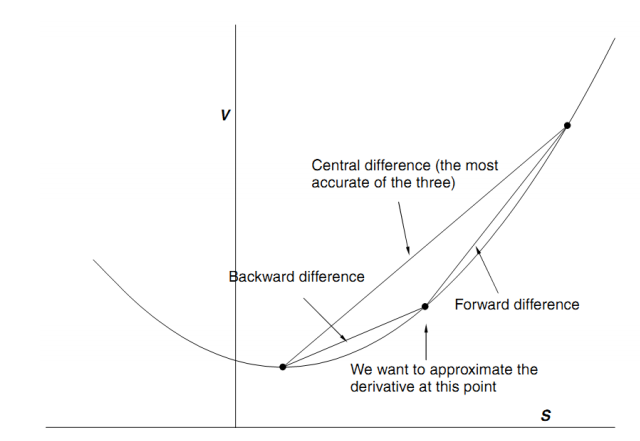
\includegraphics[width=0.7\textwidth]{figures/graph_finite_difference}
	\caption{Graphical representation of first order derivative using backward, forward and central difference.}
	\label{fig:graph_finite_difference}
\end{figure} 

\begin{table}[htb]
	\centering
	\begin{tabular}{|l|c|c|}
		\hline
		Type & Approximation & Error Order \\
		\hline
		Forward difference & $\cfrac{\partial y}{\partial x} = \cfrac{y_{i+1,j}-y_{i,j}}{\Delta x}$, $\cfrac{\partial y}{\partial t} = \cfrac{y_{i,j+1}-y_{i,j}}{\Delta x}$ & 1 \\[1ex]
		\hline
		Backward difference & $\cfrac{\partial y}{\partial x} = \cfrac{y_{i,j}-y_{i-1,j}}{\Delta x}$ & 1 \\[1ex]
		\hline
		Central difference & $\cfrac{\partial y}{\partial x} = \cfrac{y_{i+1,j}-y_{i-1,j}}{2\Delta x}$& 2 \\[1ex]
		\hline
		Second difference & $\cfrac{\partial^2 y}{\partial x^2} = \cfrac{y_{i+1,j}-2y_{i,j} + y_{i-1,j}}{\Delta x^2}$& 2 \\[1ex]
		\hline
	\end{tabular}
	\caption{Summary of derivative approximations and relative errors.}
	\label{tab:derivative_approximations}
\end{table}

These finite difference expressions are used to replace the derivatives of $y$ in the differential equation which leads to a system of $n+1$ linear algebraic equations if the differential equation is linear. If the differential equation is non-linear, the algebraic equations will also be non-linear.

Depending on which combination of presented schemes for derivatives is used in the discretization of the equation, one can end up with different approaches, \emph{explicit}, \emph{implicit} or \emph{Crank-Nicolson}. %Graphical illustration of these methods are shown with the grid in Fig.~\ref{fig:grid_finite_difference}. 
Table ~\ref{tab:various_methods} summarizes the possibilities.

%\begin{figure}[htb]
%	\centering
%	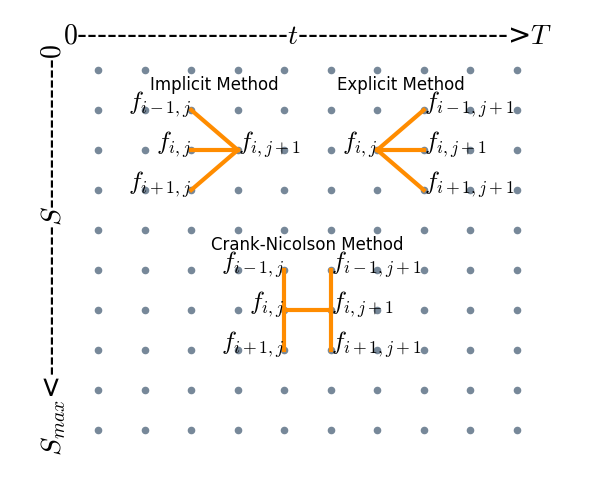
\includegraphics[width=0.7\textwidth]{figures/grid_finite_differences}
%	\caption{Example of grid used to solve an Ordinary Differential Equation.}
%	\label{fig:grid_finite_difference}
%\end{figure} 

\begin{table}[htb]
	\centering
	\begin{tabular}{|l|c|c|}
		\hline
		Method & x-derivatives & time-derivatives \\
		\hline
		Explicit & central difference & backward difference \\
		\hline
		Implicit & central difference & forward difference \\
		\hline
		Crank-Nicolson & central difference & central difference \\
		\hline
	\end{tabular}
	\caption{Possible variations of finite difference method.}
	\label{tab:various_methods}
\end{table}

Let's check an example that computes the $\Delta$ for a vanilla Interest Rate Swap when the interest rates are modelled according to the Vasicek model.

\begin{ipythonnon}
import numpy as np

r0, kappa, theta, sigma = 0.03, 0.15, 0.05, 0.03
T_max = 5.0
dt = 0.01
n_paths = 500000 
K = 0.035
pay_times = np.arange(0.5, T_max + 0.5, 0.5)

def finite_difference(r0):
  np.random.seed(42)
  n_steps = int(T_max / dt)
  r = np.full(n_paths, r0)
  integral_r = np.zeros(n_paths)
  npv = np.zeros(n_paths)

  for s in range(1, n_steps + 1):
    z = np.random.standard_normal(n_paths)
    r += kappa * (theta - r) * dt + sigma * np.sqrt(dt) * z
    integral_r += r * dt
    t = s * dt
    if any(np.isclose(t, pay_times, atol=dt/2)):
      df = np.exp(-integral_r)
      flow = (r - K) * 0.5
      npv += df * flow
  return np.mean(npv)

eps = 0.0001
price_up = finite_difference(r0 + eps)
price_dn = finite_difference(r0 - eps)
print(f"FD Delta: {(price_up - price_dn) / (2 * eps):.8f}")
\end{ipythonnon}
\begin{ioutput}
FD Delta: 3.13512801
\end{ioutput}

\subsection{Likelihood Ratio Method}
The Likelihood Ratio Method (LRM) is a powerful "Greeks" estimation technique in Monte Carlo simulations. Unlike Pathwise (Delta) methods, LRM differentiates the probability density function of the underlying process rather than the payoff itself.

This makes it particularly useful for payoffs that aren't smooth (though a vanilla swap is smooth, the logic remains the same).

Under the Vasicek model, the short rate $r_t$ follows:
\begin{equation}
dr_t=\kappa (\theta - r_t)dt+\sigma dW_t
\end{equation}

For a transition from $r_0$ to $r_T$, the density $p(r_T|r_0)$ is Gaussian. The LRM estimator for the sensitivity with respect to a parameter $\alpha$ is:
\begin{equation}
\Delta=\mathbb{E}\left[\text{Payoff}\cdot\frac{\partial\ln p(r_T|r_0)}{\partial\alpha}\right]
\end{equation}

Imagine to discretize the path in $N$ steps: $r_1, r_2,\ldots,r_N$.
The probability to observe that precise path is the product of the probabilities for each jump (Markov property):
\begin{equation}
P(r_1,\ldots,r_N|r_0)=p_1(r_1|r_0)\cdot p_2(r_2|r_1)\cdots p_N(r_N|r_{N-1})
\end{equation}

The LRM $\Delta$ is given by the expectation of the payoff multiplied by the score, or the derivative of the logarithm of the joint density w.r.t. $r_0$:
\begin{equation}
\text{Score}=\frac{\partial\log P}{\partial r_0}=\sum_{j=1}^N \frac{\partial\log p_j(r_j|r_{j-1})}{\partial r_0}
\end{equation}

At the first step, $r_1$ depends directly on $r_0$ but from the second on, $r_j$ depends on $r_{j-1}$, which in turn depends on $r_{j-2}$\ldots down to $r_0$.

For the chain rule, the derivative at each summation term is:
\begin{equation}
\frac{\partial\log p_j(r_j|r_{j-1})}{\partial r_0}=\frac{\partial\log p_j}{\partial r_j}\cdot \frac{\partial r_{j}}{\partial r_{j-1}}\cdots\frac{\partial r_1}{\partial r_0}
\end{equation}

When using a model like Vasicek where $r_j = r_{j-1}+\kappa (\theta - r_{j-1})dt$, $\frac{\partial r_j}{\partial r_{j-1}}$ equals to $(1-\kappa dt)$.
The Score at $t$ results a weighted sum of each shock along the path, with exponentially decaying weights due to mean reversion.

In a swap, cash flows are at $\{T_1, T_2,\ldots,T_k\}$ and the total value is $V=\sum\text{Payoff}(T_i)$, hence 
\begin{equation}
\Delta = \mathbb{E}\left[\sum_{i=1}^k\text{Payoff}(T_i)\cdot \text{Score}(T_i)\right]
\end{equation}

Notice that each payoff must be multiplied by the Score computed up to that time. The payoff in $T_1$ cannot be influenced by the density (hence the Score) realized between $T_1$ an $T_2$, because future doesn't influence past.

There is an issue though. In LRM  the Score in a single Euler step is proportional to 
\begin{equation}
\text{Score}_{\text{step}} \approx \frac{z}{\sigma\sqrt{dt}}
\end{equation}
where $z$ is $\mathcal{N}(0,1)$. When $dt$ becomes smaller (for a better pricing precision) the Score increases, and in the limit becomes a stochastic variable with infinitely large variance.

Adding up all the Scores for say 500 steps (5 years with $dt=0.01$), you are essentially summing variables with large oscillations. Mathematically the average should converge to the right $\Delta$ but you need a very large number of simulations.

In conclusion for a swap, LRM is correct but you should apply variance reduction techniques to increase the convergence of the Monte Carlo: \textbf{control variates} using analytic delta of a ZCB, \textbf{conditional expectation} do not use the Score at each micro-step, but only at the payment dates.

\begin{ipythonnon}
def LRM():
  np.random.seed(42)
  delta_lrm_total = 0

  for Ti in pay_times:
    exp_kTi = np.exp(-kappa * Ti)
    mean_Ti = r0 * exp_kTi + theta * (1 - exp_kTi)
    var_Ti = (sigma**2 / (2 * kappa)) * (1 - np.exp(-2 * kappa * Ti))
    std_Ti = np.sqrt(var_Ti)

    z = np.random.standard_normal(n_paths)
    r_Ti = mean_Ti + std_Ti * z

    score_r0 = ((r_Ti - mean_Ti) / var_Ti) * exp_kTi

    df = np.exp(-(r0 + r_Ti) / 2 * Ti)
    flow = (r_Ti - K) * 0.5

    payoff = df * flow
    deriv_discount = flow * df * (-Ti / 2)

    delta_lrm_total += np.mean(payoff * score_r0 + deriv_discount)

    return delta_lrm_total

print(f"LRM Delta: {LRM():.6f}")
\end{ipythonnon}
\begin{ioutput}
LRM Delta: 3.136966
\end{ioutput}

\subsection{Pathwise Method}

The Pathwise Method is a technique used in Monte Carlo simulations to calculate sensitivities (Greeks) by differentiating the payoff of a financial instrument directly along each simulated path. Unlike methods that shift the entire probability distribution, the Pathwise approach assumes that while the underlying market variables change due to a parameter shift (like a change in the initial interest rate $r_0$), the random shocks driving the simulation remain fixed. Mathematically, it applies the chain rule to the discounted payoff, requiring the payoff function to be continuous so that the derivative is well-defined.

When applied to a Vanilla Interest Rate Swap, for each payment date, the sensitivity is calculated as the sum of two distinct effects: the change in the floating rate and the change in the discount factor.

Because a shift in the initial rate $r_0$ propagates through the entire term structure—dampened by the model's mean reversion—the method tracks the "path derivative" ($\partial r_t/\partial r_0$) at every step. By aggregating these differentiated flows across all payment dates, the Pathwise method provides a high-precision Delta with significantly lower variance than other stochastic estimators, as it directly captures how the swap's Net Present Value "stretches" or "shrinks" in response to an infinitesimal move in the starting curve.

To formalize the method for a vanilla interest rate swap under the Vasicek model, we represent the Net Present Value (NPV) as the sum of $n$ discounted net cash flows.

The $\Delta$ is the expected value of the derivative of the discounted payoff with respect to the initial rate $r_0$. According to the Leibniz integral rule, we can move the derivative inside the expectation:
\begin{equation}
\Delta=\frac{\partial}{\partial r_0}\mathbb{E}\left[\sum_{i=1}^n e^{-\int_0^{T_i} r_s ds}\cdot(r_{T_i}-K)\Delta T\right]=\mathbb{E}\left[\sum_{i=1}^n\frac{\partial}{\partial r_0}(D(0,T_i)\cdot \text{Flow}_i)\right]
\end{equation}
where $D(0,T_i)$ is the stochastic discount factor and $\text{Flow}_i=(r_{T_i}-K)\Delta T$ is the cash flow at time $T_i$.

For each individual payment in the swap, we apply the product rule to account for the sensitivity of both the discount factor and the floating rate:
\begin{equation}
\frac{\partial}{\partial r_0}(D_i\cdot\text{Flow}_i)=\underbrace{D_i\cdot\frac{\partial\text{Flow}_i}{\partial r_{T_i}}\cdot\frac{\partial r_{T_i}}{\partial r_0}}_{\text{Rate Sensitivity}}+\underbrace{\text{Flow}_i\cdot\frac{\partial D_i}{\partial r_0}}_{\text{Discount Sensitivity}}
\end{equation}

In the Vasicek model, the sensitivity of the rate at any future time $t$ to the starting rate $r_0$ is deterministic and governed by the speed of mean reversion $\kappa$:

\begin{equation}
\begin{aligned}
	\frac{\partial r_t}{\partial r_0} &= e^{-\kappa t} \quad\text{(path derivative)}\\
	\frac{\partial D_i}{\partial r_0} &= D_i\cdot\left(-\int_0^{T_i}\frac{\partial r_s}{\partial r_0}ds\right) = D_i\cdot\left(-\int_0^{T_i}e^{-\kappa s}ds\right)\quad\text{(discount derivative)}
\end{aligned}
\end{equation}

Combining these, the Pathwise Delta for the entire swap is computed along each simulated path as:
\begin{equation}
\Delta = \sum_{i=1}^n D(0,T_i)\Delta T\left[e^{-\kappa T_i}-(r_{T_i}-K)\left(\frac{1-e^{-\kappa T_i}}{\kappa}\right)\right]
\end{equation}

This formula explains why the method is so stable: it avoids the $1/\sqrt{dt}$ terms found in LRM and instead uses the smooth, exponential decay of the Vasicek mean-reversion process.

\begin{ipythonnon}
def pathwise(r0):
  np.random.seed(42)
  n_steps = int(T_max / dt)
  r = np.full(n_paths, r0)

  integral_r = np.zeros(n_paths)
  npv = np.zeros(n_paths)

  path_deriv = np.ones(n_paths)
  integral_path_deriv = np.zeros(n_paths)
  delta_pw_acc = np.zeros(n_paths)

  for s in range(1, n_steps + 1):
    z = np.random.standard_normal(n_paths)

    path_deriv += -kappa * path_deriv * dt
    integral_path_deriv += path_deriv * dt

    r += kappa * (theta - r) * dt + sigma * np.sqrt(dt) * z
    integral_r += r * dt

    t = s * dt
    if any(np.isclose(t, pay_times, atol=dt/2)):
      df = np.exp(-integral_r)
      flow = (r - K) * 0.5
      npv += df * flow

      d_df = df * (-integral_path_deriv)
      d_flow = path_deriv * 0.5
      delta_pw_acc += (d_df * flow + df * d_flow)
  return np.mean(delta_pw_acc)

print(f"PW Delta: {pathwise(r0):.8f}")        
\end{ipythonnon}
\begin{ioutput}
PW Delta: 3.13512794
\end{ioutput}

\subsubsection{Technique Comparison}

The numerical results reported in the previous sections referred to a single MC with 100000 simulations for each method and the results were consistent.
To improve a Monte Carlo simulation means to achieve the same level of precision with a smaller number of trials, \emph{convergence acceleration}.
Hence it is interesting to look at the convergence plot, i.e. $\Delta$ versus number of simulations, Fig.~\ref{fig:MC_greek_comparison}.

\begin{figure}[htb]
	\centering
	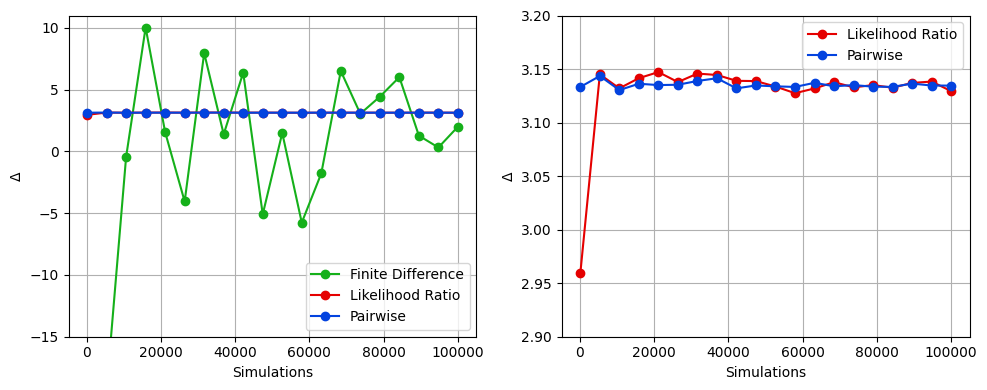
\includegraphics[width=0.9\textwidth]{figures/mc_greek_comparison}
	\caption{Left plot compares the three methods. Right plot shows with a finer detailed Pairwise and Likelihood Ratio results.}
	\label{fig:MC_greek_comparison}
\end{figure}

From the left plot it is apparent how Likelihood Ratio and Pairwise technique outperform the simpler finite difference, from the right one instead we can see that, at least for the IRS case, the Pairwise is slightly better than the LR. % da riguardare
%\include{hjm}
\chapter{Credit Risk}\label{credit_default_swaps}

Credit risk is the possibility of a loss resulting from a borrower's failure to repay a loan or meet contractual obligations. Traditionally, it refers to the risk that a lender may not receive the owed principal and interests, which results in an interruption of cash-flows and increased costs for collection. 

Although it's impossible to know exactly who will default on obligations, properly assessing and managing credit risk can lessen the severity of a loss. Interest payments from the borrower or issuer of a debt obligation are a lender's or investor's reward for assuming credit risk.

In this Chapter the definition of credit event is introduced together with the Credit Default Swaps, a new type of instrument whose value depends on the likelihood that a given company will suffer a credit event over a given period.

\section{Credit curves}
\label{credit-curves}

A \emph{credit event} can be a default, the failure to make payments, the issuer entering into bankruptcy proceedings, or the occurrence of other legal events. The exact definition of what constitutes a credit event depends on a series of factors and is usually defined in some kind of ISDA (International Swaps and Derivatives Association) master agreement. In any case in the rest of these notes, with credit event we will mean a \emph{default}.

\emph{Non-default probability} (NDP or survival probability) is the probability that a company will not suffer a credit event \textbf{before} a given date, i.e. non-default probability is a cumulative probability.

\emph{Credit curves} are a way of representing survival probabilities, and just like discount curves, they are built by specifying a sequence of pillar dates to which corresponds a sequence of NDPs. 

\begin{finmarkets}
	Similarly to discount curves we implement a class to handle credit curves, \texttt{CreditCurve}. It is characterized by a list of pillar dates with the corresponding survival probabilities. Like the \texttt{DiscountCurve} object you don't need to pass the observation date value (survival probability 1) since it is done automatically by the class constructor. Two methods are available: one to interpolate survival probabilities and the second to compute the hazard rate at any arbitrary date (beware that extrapolation is not allowed so the input date must be within the pillar dates range).
\end{finmarkets}

\pythoncodenon{code/credit_risk_credit_curve.py}
Let's test the class with some inputs.
\begin{ipythonnon}
from dates import GlobalConst as gc, TimeInterval
from curves import CreditCurve

cc = CreditCurve([ gc.OBS_DATE + relativedelta(years=2)], [0.8])

print (cc.ndp( gc.OBS_DATE + TimeInterval("1y")))
print (cc.hazard( gc.OBS_DATE + TimeInterval("1y")))
\end{ipythonnon}
\begin{ioutput}
0.9
0.11111111111112416
\end{ioutput}

\subsection{Credit Event Simulation}
\label{sec:credit_event_simulation}
The simplest way to simulate possible default is to use the $\texttt{scipy.stats.binom.rvs(n, p, size)}$ function:
\begin{itemize}
	\item default is a binary process: a borrower either defaults or do not with default probability $\Pdef$;
	\item instead of generating $n$ individual random numbers in a loop to check each borrower's fate, $\texttt{scipy.stats.binom}$ samples the total count of defaults directly from the theoretical distribution in a single, optimized operation;
	\item with multiple \textbf{independent} counterparties we can simulate their defaults at once specifying each different ${\Pdef}^i$.
\end{itemize}	

As an example let's consider 10 firms with 10\% default probability each and compute the probability of having 5 defaults within the next year.
\begin{ipythonnon}
import numpy as np

from scipy.stats import binom

np.random.seed(1)

n_assets = 10
PD = np.ones(shape=(n_assets,)) * 0.1

N = 1000000

defaults = binom.rvs(1, PD, size=(N, n_assets)) # simulate N default scenarios
print ("Simulated defaults (first 5 simulations):")
print (defaults[:5])

outcomes = np.sum(defaults, axis=1) # compute number of defaults per scenario
print ("\nTotal defaults per simulation:")
print (outcomes[:5])

successes = (outcomes >= 5)
print ("\nSimulation with >= 5 defaults:")
print (successes[:5].astype(int))

print (f"\nP(ndefs >=5): {np.mean(successes)}")
\end{ipythonnon}
\begin{ioutput}
Simulated defaults (first 5 simulations):
[[0 0 0 0 0 0 0 0 0 0]
[0 0 0 0 0 0 0 0 0 0]
[0 1 0 0 0 0 0 0 0 0]
[0 0 1 0 0 0 0 0 0 0]
[1 0 0 0 0 0 1 0 0 0]]

Total defaults per simulation:
[0 0 1 1 2]

Simulation with >= 5 defaults:
[0 0 0 0 0]

Probability of having at least 5 uncorrelated defaults: 0.00166
\end{ioutput}

We can check the correctness of the result by saying that to get at least 5 defaults out of 10 assets we need to have (at least) 5 defaults and 5 no-defaults, so the probability is $\Pdef^5$ times $\Psur^5$ times the number
of ways in which I can choose 5 defaulting assets out of ten (combinations $\binom{10}{5}=252$):
\begin{equation*}
\Pdef(5) > (0.1)^5 \cdot (0.9)^5 \cdot 252 \approx 0.0015
\end{equation*}

This number doesn't exactly match the MC simulation since the calculation doesn't consider the case with 6 and more defaults, but it gives the correct order of magnitude though.

\subsection{Hazard Rate or Default Intensity}
\label{hazard-rate}

The \emph{hazard rate}~\cite{bib:hazard} represents the instantaneous probability of a party defaulting conditioned on it not having defaulted until that moment. Indeed it is often called a \emph{conditional failure rate} since its expression is a direct application of the conditional probability concept, see Section~\ref{sec:conditional_prob}.

Let $\tau$ be the random time of default, with a cumulative distribution function $\Pdef(t) = \mathbb{P}(\tau \le t)$ and a probability density function $f(t) = \frac{d\Pdef(t)}{dt}$.
The probability of surviving past time $t$ is:
$$\Psur(t) = \mathbb{P}(\tau > t) = 1 - \Pdef(t)$$
We look at the probability of defaulting between $t$ and $t + \Delta t$ conditioned on survival up to $t$:
$$\mathbb{P}(t < \tau \le t + \Delta t \mid \tau > t) = \frac{\mathbb{P}((t < \tau \le t + \Delta t) \cap (\tau > t))}{\mathbb{P}(\tau > t)}$$
Since the event $\{t < \tau \le t + \Delta t\}$ is a subset of $\{\tau > t\}$, their intersection simplifies to $\mathbb{P}(t < \tau \le t + \Delta t)$. Expressing this in terms of the CDF and the survival function $\Psur(t)$:
$$\mathbb{P}(t < \tau \le t + \Delta t \mid \tau > t) = \frac{\Pdef(t + \Delta t) - \Pdef(t)}{\Psur(t)}$$
To find the instantaneous rate per unit of time, we divide by the interval length $\Delta t$ and take the limit as $\Delta t \to 0$:

$$\lambda(t) = \lim_{\Delta t \to 0} \frac{\mathbb{P}(t < \tau \le t + \Delta t \mid \tau > t)}{\Delta t} = \lim_{\Delta t \to 0} \frac{\Pdef(t + \Delta t) - \Pdef(t)}{\Delta t \cdot \Psur(t)}$$
Factoring out $\Psur(t)$ (which does not depend on $\Delta t$), the limit of the numerator is precisely the probability density function $d\Pdef(t)/dt$:

$$\lambda(t) = -\frac{1}{P_{\text{sur}}(t)} \frac{dP_{\text{sur}}(t)}{dt} = -\frac{d}{dt} \ln P_{\text{sur}}(t)$$
Given the hazard rate, the survival probability can be determined as:
\begin{equation}
\begin{gathered}
\lambda(t) = -\cfrac{1}{dt}\cdot\cfrac{d\Psur(t_0, t)}{\Psur(t_0, t)} = -\cfrac{d(\log\Psur(t_0, t))}{dt} \implies d(\log\Psur(t_0, t)) = -\lambda dt\\[5pt]
\Psur(t_0, t) = \mathrm{exp}\left(-\int_{t_0}^{t}\lambda(s) ds\right)
\end{gathered}
\label{eq:constant_hazard_rate_prob}
\end{equation}

In practice hazard rate will be calculated numerically, and therefore we will consider the \emph{annualized} conditional probability of the issuer defaulting between a date and the next.

\label{sec:constant_hazard_rate}
The simplest possible survival distribution is obtained by assuming a constant risk over time, so the hazard is $\lambda (t)=\lambda$ for all $t$. The corresponding survival function is $\Psur(t_0, t) = e^{-\lambda (t-t_0)}$.

\subsection{Poisson Process}
\label{sec:poisson_process}

The kind of processes described by Eqs.~\ref{eq:constant_hazard_rate_prob} belong to a class of models called \emph{Poisson processes}. 
They can be used to model the frequency of events during a certain period of time assuming that one knows the average occurrence of those events. An alternative derivation of the same formulas will give us interesting insights on how it would be possible to simulate default times.

Consider random events such as the arrival of customer at a shop, or the arrival of emails to a mail server or the arrival of calls to a call-center. These events can be described by a counting function $N(t)$ defined for all $t\ge 0$.

This counting function represents the number of events that occurred in $[0, t]$. For each interval $[0,t]$ the value $N(t)$ is an observation of a random variable where the only possible values are the integers $0, 1, 2\ldots$

The counting process $\{N(t):t\ge 0\}$ is said to be a \emph{Poisson process} with mean rate $\lambda$ if the following assumptions are fulfilled:
\begin{itemize}
\item $N(0)=0$;
\item it has independent increments: that is the number of arrivals during non-overlapping time intervals are independent random variables;
\item the number of events in any interval of length $t$ is a Poisson random variable with parameter $\lambda t$.
\end{itemize}

Therefore
\begin{equation}
P(N(t)=n)=\cfrac{e^{-\lambda t}(\lambda t)^n}{n!}
\label{eq:poisson_pdf}
\end{equation}

The last assumption implies that the distribution of the number of arrivals between, say, $t$ and $t+s$ depends only on the length of the interval $s$ and not on the starting point $t$. This property is usually called \emph{stationarity}. Consequently:
\begin{equation}
P(N(t)-N(s)=n)=\cfrac{e^{-\lambda (t-s)}(\lambda (t-s))^n}{n!}
\end{equation}

and because of the properties of the Poisson distribution:
\begin{equation}
\mathbb{E}[N(t)-N(s)]=\lambda (t-s)
\end{equation}

Now consider the time at which arrivals occurs in a Poisson process. Let the first arrival occur at time $T_1$, the second occur at time $T_1 + T_2$ and so on. Thus $T_1$, $T_2, \ldots$ are successive \emph{inter-arrival times}. The first arrival occurs after time $t$ if and only if there are no arrivals in the interval $[0,t]$ so 
\begin{equation}
\{T_1>t\}=\{N(t)=0\}
\end{equation}
and consequently
\begin{equation}
P(T_1>t)=P(N(t)=0)=e^{-\lambda t}
\end{equation}

Thus the probability that the first arrival will occur in $[0,t]$ is given by
\begin{equation}
P(T_1\le t)= 1-P(T_1>t)=1-e^{-\lambda t}
\end{equation}
which is the same function obtained for the default probability in case of constant hazard rate, see~\ref{sec:constant_hazard_rate}.

Recall that CDF of $X$ returns the probability that the interval of time between consecutive events will be less than or equal to some value $t$.
Hence, $T_1$ is distributed exponentially
\begin{equation}
P_{T_1}(t) = \cfrac{d}{dt}(1-e^{-\lambda t}) = \lambda e^{-\lambda t}
\end{equation}
with mean  
\begin{equation}
\mathbb{E}[P_{T_1}(t)] = \cfrac{1}{\lambda}
\end{equation}
It can also be shown that all inter-arrival times $T_1, T_2,\ldots$ are exponentially distributed and independent with mean $1/\lambda$.

Finally the inverse function of the CDF is:
\begin{equation}
F^{-1}(X) = -\frac{\log(1-X)}{\lambda}
\end{equation}

A constant hazard rate ($\lambda$) implies that the probability of defaulting in the next instant, given that the entity has survived until now, is exactly the same regardless of whether the entity is 1 day old or 20 years old.

In the real world, this is considered unrealistic for several key reasons:
\begin{itemize}
	\item the "Aging" Effect (Credit Quality Dynamics): a constant hazard rate follows a memoryless property. It assumes that the entity's history or current age provides no information about its future stability. In reality, as a company matures, it typically builds retained earnings, establishes market share, and stabilizes its capital structure, which might lower its default risk over time. Conversely, a startup has a much higher "infant mortality" rate.
	\item the Credit Cycle and Macroeconomics: default risk is heavily tied to the economic cycle (recessions vs. expansions). Hazard rates are stochastic and time-dependent. We expect default risk to be higher during a projected downturn in 2 years than it might be in the current stable month. A constant $\lambda$ cannot capture the "mean-reverting" nature of economic conditions.
	\item Term Structure of Credit Spreads: If you look at the market prices for Credit Default Swaps (CDS) or corporate bonds, the "Credit Curve" is rarely flat.    \textit{Upward Sloping}: investors often demand a higher premium for longer maturities because there is more uncertainty about the distant future (e.g., the company might face new competitors or technological obsolescence). \textit{Downward Sloping}: for distressed entities, the risk of defaulting now (liquidity crisis) is often much higher than the risk of defaulting in 5 years if they manage to survive the current quarter. Constant Hazard Rate results in a perfectly flat credit curve, which almost never matches market data.
	\item Information Dissipation: the longer an entity survives, the more information the market has about its management and resilience. A constant hazard rate ignores the fact that survival itself acts as a signal of quality. In many models (like those using the Lévy process or Structural models), the probability density of default changes as the entity's asset value moves relative to its "default barrier."
\end{itemize}

So in conclusion most entities follow a \textit{Bathtub Curve}: high risk at the start (startups), low, relatively constant risk in the middle and increasing risk as the entity or industry becomes obsolete.

The simplest improvement to account for the previous consideration in the credit risk modeling is to consider a \textbf{piecewise constant $\lambda$}.

\begin{finmarkets}
We now have enough information to simulate credit events according to a Poisson process. 

The following class is an \emph{extension} of \texttt{scipy.stats} that implements distributions of the form $\lambda e^{-\lambda t}$. %This is another example of \emph{sub-classing} an existing class (for inheritance, see Section~\ref{inheritance-and-overriding-methods}) since its parent is \texttt{rv\_continuous} the starting point for each continuous distribution in \texttt{scipy}.

Once the default intensity has been set, we can model the cumulative default probability over a certain period of time using the \texttt{cdf} method. Contrary feeding different probability values, using the inverse-CDF (the \texttt{ppf} method), gives us the corresponding default times for the respective probabilities.
Default times can also be obtained by sampling from the distribution as shown in the next example.
\end{finmarkets}

\pythoncodenon{code/credit_risk_poisson_process.py}
Let's plot the distribution of the arrival time of events described by a Poisson process with constant $\lambda=5$, see Figure~\ref{fig:default_time_simulation}.

\pythoncodenon{code/credit_risk_poisson_process_mc.py}

\begin{figure}[htb]
	\centering
	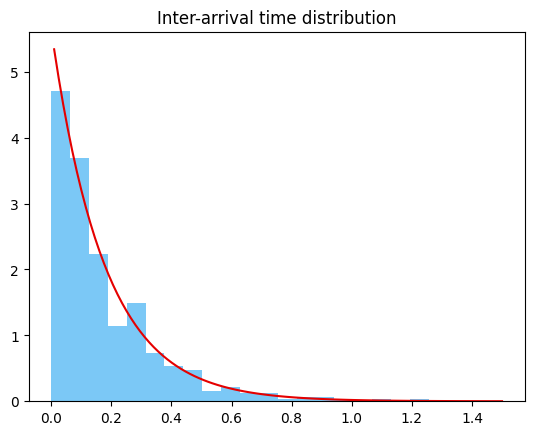
\includegraphics[width=0.7\textwidth]{figures/default_time_simulation}
	\caption{Default times simulated through the sampling from a Poisson process with $\lambda=5$ and time interval $t=100$. An exponential fit shows that the decay rate is about $1/\lambda=0.2$.}
	\label{fig:default_time_simulation}
\end{figure}

\subsubsection{Calibration Example}

To calibrate the such a Poisson process to a non-flat market credit curve, we need to find the set of $\lambda$ values that make the model's survival probabilities match the market's implied survival probabilities at specific pillar dates.

Although this is typically done using a bootstrapping process, here we are going to use a global optimization approach (e.g. least squares). 
In the example below the function \texttt{calibrate} takes market pillar dates and their corresponding market survival probabilities and will use \texttt{scipy.optimize.least\_squares} to solve for the hazard rates.

\begin{ipythonnon}
from scipy.optimize import least_squares

from distributions import PoissonProcess

def calibrate_credit_process(market_times, market_probs, initial_guess=0.02):
  times = np.array(market_times)
  probs = np.array(market_probs)
    
  def residuals(log_lambdas):
    temp_lambdas = np.exp(log_lambdas)
    temp_process = PoissonProcess(temp_lambdas, times)
    return temp_process.survival_prob(times) - probs

  x0 = np.log(np.ones(len(times)) * initial_guess)
  sol = least_squares(residuals, x0, method='lm')   
  if not sol.success:
    raise ValueError("Calibration failed to converge")

  return PoissonProcess(np.exp(sol.x), times)
\end{ipythonnon}

When you run this calibration, you'll see that lambda values are no longer identical. This allows the model to "bend" the survival curve to fit market expectations. For example if the 1Y hazard rate is higher than the 5Y rate, the market is pricing immediate distress. Also if the rates increase over time, the market sees the entity as safe now but potentially risky in the long run.

Suppose you have CDS market data that implies the following survival probabilities (usually derived from CDS spreads): 1Y 98\% survival, 3Y 92\% survival and 5Y 85\% survival.

\begin{ipythonnon}
t_market = [1, 3, 5, 10]
p_market = [0.99, 0.95, 0.88, 0.70] 
	
calibrated_model = calibrate_credit_process(t_market, p_market)
	
print("Calibrated Lambdas:", calibrated_model.lambdas)
print(f"Prob at 5Y: {calibrated_model.survival_prob(5.0):.2%}")
\end{ipythonnon}
\begin{ioutput}
Calibrated Lambdas: [0.01005034 0.02062148 0.03827004 0.04576831]
Prob at 5Y: 80.00%
\end{ioutput}

Because the hazard rate is piecewise constant, the default PDF will have visible \textit{jumps} at the pillar dates (1Y, 3Y, 5Y). While this looks strange on a graph, it is the industry standard because it makes the math of pricing instruments like CDS very fast and consistent, as we will see in the next Section.

\section{Credit Default Swaps}
\label{sec:credit-default-swaps}

A Credit Default Swap (CDS) is a financial agreement in which the seller commits to compensate the buyer in case of a default or other credit event. That is, the seller of the CDS "insures" the buyer against some reference asset defaulting. In exchange the buyer of the CDS makes a series of payments (the CDS \emph{spread}) to the seller.

\subsection{Valuation of CDS}
\label{sec:cds_valuation}

Credit Default Swaps are made up of two legs:

\begin{itemize}
\tightlist
\item \emph{premium} leg: which pays the spread $S$ periodically until a credit event occurs;
\item \emph{default} leg: which pays $L = F(1 - R)$, known as the \textbf{loss given default} (LGD), if and when the credit event occurs ($F$ is the notional of the contract, $R$ is the \textbf{recovery rate} or the percentage of the loss recovered from a default. The recovery rate varies by industry, the degree of seniority in the capital structure, the amount of leverage in the capital structure in total, and whether a particular security is secured or otherwise collateralized. A common baseline assumption is to set it to 40\%.
\end{itemize}

\subsubsection{Premium leg}\label{premium-leg}

In the valuation of the premium leg, we'll use the following notation:

\begin{itemize}
\tightlist
\item $d$ pricing date;
\item $d_0$ the start date of the CDS (could be different from pricing date);
\item $d_1, ..., d_n$ the payment dates of the premium leg. We assume that $d_n$ is the end date of the CDS;
\item $D(d')$ the discount factor between $d$ and $d'$;
\item $\Psur(d, d')$ the survival probability between $d$ and $d'$;
\item $\tau$ the \emph{random variable} representing the credit event date.
\end{itemize}

At each payment date $d_i$, a cash flow of $F\cdot S$ is paid if and only if the credit event has \emph{not} occurred before that date. Therefore the NPV of each flow is

\begin{equation}
f_{\textrm{premium}}^i = \mathbb{E}\left[F\cdot S\cdot D(d_i)|\mathbbm{1}(\tau > d_i) \right]
\end{equation}
where the indicator function $\mathbbm{1}(\tau > d_i)$ means that the expectation value has to be evaluated when $\tau > d_i$. 

Since the NPV depends on the random variable $\tau$, the estimate of its value needs to be done through an expectation.
Remembering the definition of expected value (see Section~\ref{sec:expected-value}), %we can interpret 
%\(F\cdot S\cdot D(d_i)\) as the variables and $\Psur(d, d_i)$ as the probabilities so 
the premium leg NPV can be expressed as:

\begin{equation}
\textrm{NPV}_{premium} = F\cdot S \cdot \sum_{i=1}^{n} D(d_i) \cdot \Psur(d, d_i)\frac{d_i-d_{i-1}}{365}
\end{equation}

\subsubsection{Default leg}
\label{default-leg}

We assume that as soon as a credit event occurs (at a time $\tau$) the LGD is paid out (i.e. on the same date, but could potentially be paid on any date between $d_0$ and $d_n$). Mathematically, therefore, the NPV of the default leg can be expressed as follows:

\begin{equation}
\mathrm{NPV_{default}} =\mathbb{E}[F(1-R)\cdot D(\tau)|\mathbbm{1} \{\tau \leq d_n\} ] = \mathbb{E}[F(1-R)\cdot D(\tau)|\Pdef(\tau \leq d_n) ]
\end{equation}

Also in this case we are dealing with a probabilistic event so the expectation value has to be computed taking into account the payments $F(1-R)\cdot D(\tau)$ averaged over the default probability $\Pdef(d, \tau)$. 

Using the law of total probability (see~\ref{sec:conditional_prob}), we can break the previous expression down into the sum of "daily NPVs" calculated as a function of the \emph{daily} default probabilities:

\begin{align}
\begin{split}
\mathrm{NPV_{default}} &= \mathbb{E}[F(1-R)\cdot D(\tau)|\Pdef(\tau \leq d_n) ] = \sum_{d'=d_0}^{d_n} \mathbb{E}[F(1-R) \cdot D(d')|\Pdef(d, d')] \\
&= F(1-R) \sum_{d'=d_0}^{d_n} D(d') \left(\Pdef(\tau \geq d') - \Pdef( \tau \geq d'+1) \right) \\
&= F(1-R) \sum_{d'=d_0}^{d_n} D(d') \left(\Psur(d, d') - \Psur(d, d'+1) \right)
\end{split}
\end{align}
where the last step holds since $\Pdef(\tau\geq d') = 1 - \Pdef(\tau < d') = 1 - (1-\Psur(d, d')) = \Psur(d, d')$. 
Figure~\ref{fig:default_p} illustrates the steps to convert the daily default probability $\Pdef(d, d')$.

\begin{figure}[htb]
\centering
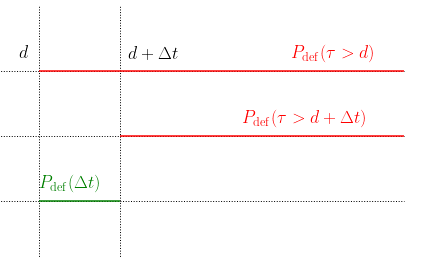
\includegraphics[width=0.7\textwidth]{figures/timeline}
\caption{The probability that a default occurs at a time $\tau = d+\Delta t$ is equivalent to the default probability at $\tau > d$ minus the default probability at $\tau>d+\Delta t$.}
\label{fig:default_p}
\end{figure}

\begin{finmarkets}
As for the other kind of contracts we develop also a \texttt{CreditDefaultSwap} class. In this case the class has methods to compute NPVs for two legs and the break-even spread.

The break-even spread of a credit default swap is the value of the fixed rate paid in the premium leg that makes the CDS net present value equal to 0.

To determine the break-even spread is enough to impose that the NPV of the premium and default legs are equal:

\begin{equation}
S \cdot\sum_{i=1}^{n} D(d_i) \cdot \Psur(d, d_i)
= (1-R) \sum_{d'=d_0}^{d_n} D(d') \left(\Psur(d, d') - \Psur(d, d'+1) \right)
\end{equation}
solving for $S$ we obtain the wanted spread

\begin{equation}
S_{\mathrm{breakeven}} = \cfrac{(1-R) \sum_{d'=d_0}^{d_n} D(d') \left(\Psur(d, d') - \Psur(d, d'+1) \right)}{\sum_{i=1}^{n} D(d_i) \cdot \Psur(d, d_i)}
\end{equation}
\end{finmarkets}

\pythoncodenon{code/credit_risk_cds.py}

To test the class data contained in \href{https://github.com/matteosan1/finance_course/raw/master/input_files/discount_factors_2022-10-05.xlsx}{discount\_factors\_2022-10-05.xlsx} is used.

\begin{ipythonnon}
import pandas as pd

from dates import GlobalConsts as gc, TimeInterval
from curves import DiscountCurve
from credit import CreditDefaultSwap

dc_data = pd.read_excel("discount_curve.xlsx")
dates = [gc.OBS_DATE + TimeInterval(i) for i in dc_data['maturities']]
dc = DiscountCurve(dates, dc_data['dfs'])

pillars = [gc.OBS_DATE + TimeInterval('36m')]
credit_curve = CreditCurve(pillars, [0.7])
cds = CreditDefaultSwap(1e6, gc.OBS_DATE, "3y", 0.03)

print (f"NPV premium leg: {cds.npv_premium_leg(dc, credit_curve):.2f}")
print (f"NPV default leg: {cds.npv_default_leg(dc, credit_curve):.2f}")
print (f"NPV CDS: {cds.npv(dc, credit_curve):.2f}")
\end{ipythonnon}
\begin{ioutput}
NPV premium leg: 75761.20
NPV default leg: 180902.43
NPV CDS: 105141.23
\end{ioutput}
	
\begin{finmarkets}
An alternative implementation of the default leg calculation (i.e. \texttt{npv\_default\_leg} method) is possible. The explicit daily loop over the lifetime of the swap could indeed be replaced by a numerical intergral between $[t_0, T]$.
The code below provide an example exploiting the integration function \texttt{scipy.integrate.quad}. For more information about integration in \texttt{python} please refer to Section~\ref{sec:integration}.

\begin{ipythonnon}
from scipy.integrate import quad

def npv_default_leg_quad(self, cc, dc):
  def integrand(t, cc, dc):
    current_date = self.payment_dates[0] + \ 
                   TimeInterval(f"{int(t * 365)}d"))
	return dc.df(current_date) * (cc.ndp(current_date) \
                  - cc.ndp(current_date + TimeInterval("1d")))
  maturity_in_years = yearFraction(self.payment_dates[0], 
                                   self.payment_dates[-1])
  npv, _ = quad(integrand, 0, maturity_in_years, args=(cc, dc))
  return self.nominal * (1 - self.recovery) * npv * 365
\end{ipythonnon}

This new approach provide a higher precision and is often faster especially for long swap maturities, although it requires a little overhead in converting at each step the year fraction into an actual date.

Furthermore if your credit curve uses a piecewise constant hazard rate ($\lambda$), you don't actually need numerical integration at all. Indeed within each segment where $\lambda$ is constant, the integral has a closed-form solution:

\begin{equation}
\int_{t_1}^{t_2} e^{-rt} \lambda e^{-\lambda t} dt = \frac{\lambda}{r +\lambda} \left(e^{-(r+\lambda)t_1}-e^{-(r+\lambda)t_2}\right)
\end{equation}

Using this summation across the "buckets" of your credit curve is the industry standard for CDS pricing because it is mathematically exact and near instantaneous.
\end{finmarkets}


%\section{Credit Ratings}\label{credit-ratings}
%
%A credit rating is a quantified assessment of the creditworthiness of a borrower either in general terms or with respect to a particular debt or financial obligation. A credit rating can be assigned to any entity that seeks to borrow money (e.g. an individual, corporation, state or provincial authority, or sovereign government).
%
%A loan is a essentially a promise and the credit rating determines the likelihood that the borrower will be able to pay back it within the loan agreement terms. A high credit rating indicates a high possibility of paying back the loan in its entirety without any issue; a poor credit rating suggests that the borrower has had trouble paying back loans in the past and might follow the same pattern in the future.
%
%Individual credit is scored from credit bureaus (e.g. Experian and TransUnion) and it is reported as a number, generally ranging from 300 to 850.
%
%Credit assessment and evaluation for companies and governments instead is generally done by credit rating agencies (e.g. Standard \& Poor's (S\&P), Moody's, or Fitch), which typically assign letter grades to indicate ratings. Standard \& Poor's, for instance, has a credit rating scale ranging from AAA (excellent) to C and D. A debt instrument with a rating below BB is considered to be a speculative grade or a junk bond, which means it is more likely to default on loans.
%
%\subsection{Why Credit Ratings Are Important}\label{why-credit-ratings-are-important}
%
%A borrowing entity will strive to have the highest possible credit rating since it has a major impact on interest rates charged by lenders. Rating agencies, on the other hand, must take a balanced and objective view of the borrower's financial situation and capacity to repay the debt.
%
%A credit rating not only determines whether or not a borrower will be approved for a loan but also determines the interest rate at which the loan will need to be repaid. Since companies depend on loans for many expenses, being denied a loan could spell disaster, and in any case a high interest rate is much more difficult to pay back.
%Credit ratings also play a large role in a potential investor's determining whether or not to purchase bonds. A poor credit rating is a risky investment; it indicates a larger probability that the company will be unable to make its bond payments.
%
%It is important for a borrower to remain diligent in maintaining a high credit rating. Credit ratings are never static; in fact, they change all the time based on the newest data, and one negative debt will bring down even the best score. 
%Credit also takes time to build up. An entity with good credit but a short credit history is not seen as positively as another entity with the same quality of credit but a longer history. Debtors want to know a borrower can maintain good credit consistently over time.

\section{Determine Default Probabilities from Market Quotes}
In this Section we find out how to derive default probabilities implied by market quotes, checking how it can be done both from bonds and Credit Default Swaps.

\subsection{Default Probability from Bonds}
\label{default-probabilities-and-bond-prices}

The price of a bond issued by a party is directly linked to the credit rating of that party, since there is always an associated default risk (the borrower might not be able to repay fully or partially the amount of the taken loan). 

Bonds with low ratings, called junk bonds, are sold at lower prices (since riskier), while those with higher ratings, called investment-grade bonds, are sold at higher prices.

The average default intensity can be approximated by considering the spread $s$ between the rates of a risky and a risk-free bond, and the recovery rate $R$.

The risk-free zero coupon bond value $e^{-(r+s)\cdot T}$ equals that of the risky bond which can be computed remembering the expression for the default probability as a function of the hazard rate when this is constant (see Example~\ref{sec:constant_hazard_rate})

\begin{equation}
e^{-(r+s)\cdot T} = 
\begin{cases}
R\;\;\textrm{with probability}\;1 - e^{-\lambda T} \\
1\;\;\textrm{with probability}\;e^{-\lambda T} \\
\end{cases} = 
(e^{-\lambda T} + R - R e^{-\lambda T})e^{-rT}
\end{equation}

If $\lambda$ is small we can use the Taylor expansion neglecting orders higher than the first $e^{x} = 1 + x$ (the discount factor can be simplified away from both sides)

\begin{equation}
\begin{gathered}
e^{-sT} = e^{-\lambda T} + R - R e^{-\lambda T} \\
1 - sT = 1 - \lambda T + R - R(1 - \lambda T) = 1 - \lambda T + R - R + R\lambda T\\
\end{gathered}
\end{equation}
Simplifying and changing signs we are left with
\begin{equation}
s = (1 - R)\cdot \lambda \implies \lambda = \frac{s}{1-R}
\end{equation}

Imagine for example a bond that yields 150 basis points more than a similar risk-free bond and assume an expected recovery rate of 40\%.

\begin{equation*}
\bar{\lambda} = \cfrac{0.015}{(1-0.4)} = 2.5\%
\end{equation*}

% \subsubsection{Better Approximation}

% To estimate the default probability with a higher precision is possible to calculate the expected loss in terms of the unconditional default probability $Q$. As before

% \begin{equation}
% Q = \cfrac{s}{\sum\mathrm{expected\_losses}}
% \end{equation}
% where $s$ is now the difference in price between the risky and the risk-free bonds.

% Consider a 5-year corporate bond which provides an annual 6\% coupon (paid semiannually), with an yield of 7\%. The yield of a similar risk-free bond is instead 5\%. Assume a recovery rate of 40\% and that defaults can happen only immediately before coupon payment dates at times 0.5, 1.5, 2.5, 3.5 and 4.5. 

% Let's determine the unconditional default probability $Q$ in \texttt{python}.

% \begin{ipython}
% from math import exp
% import numpy as np

% default_dates = [0.5, 1.5, 2.5, 3.5, 4.5]
% R = 0.4

% def bond_price(N, C, y, maturity, tenor):
%     val = 0
%     for i in np.arange(tenor, maturity+tenor, tenor):
%         val += N*C*tenor*exp(-y*i)
%     val += N*exp(-y*i)
%     return val

% def expected_loss(N, C, r, maturity, tenor):
%     loss = 0
%     for i in range(len(default_dates)):
%         val = 0
%         for t in np.arange(default_dates[i], maturity+tenor, tenor):
%             val += N*C*tenor*exp(-r*(t-default_dates[i]))
%         val += N * exp(-r*(t-default_dates[i]))
%         val = (val-N*R)*exp(-r*default_dates[i])
%         loss += val
%     return loss

% Pr = bond_price(100, 0.06, 0.07, 5, 0.5)
% Prf = bond_price(100, 0.06, 0.05, 5, 0.5)
% spread = abs(Pr - Prf)
% print ("{:.2f}%".format(spread / expected_loss(100, 0.06, 0.05, 5, 0.5)*100))
% \end{ipython}
% \begin{ioutput}
% 3.03%
% \end{ioutput}

% This algorithm can be generalized for example by defining $Q$ as a function of the hazard rate. By using several bonds with different maturities also it is possible to derive the term structure of the default probability with an approach similar to the bootstrap.

%Let's see with an example how the default probability can be determined from bond prices. Imagine to have a bond and let \(x\) represent the present value of its cash flow stream. To valuate the bond when a default probability is associated to the issuer it is necessary to take each possible value of $x$ (the value of the bond), multiply it by the corresponding default probability and sum the results.  In other words the value of the bond should equal the mathematical expectation (see Section~\ref{sec:expected-value}) of $x$.
%
%Consider a bond which pays $F$ at maturity and that the issuer of this bond has a default probability $P$ (the recovery is $R$). What will be the price of this bond ?
%
%\begin{equation}
%V_{bond} =
%\begin{cases}
%& D \cdot R \cdot F\quad\textrm{(in case of default of the issuer)}\\
%&D \cdot F\quad\textrm{(in case of no default)}\\
%\end{cases}\end{equation} 
%where \(D\) is the proper discount factor. Since we don't
%know if the issuer will default or not we can estimate the bond price as
%
%\begin{equation}
%V_{bond} = D \cdot R \cdot F \cdot DP ( \tau ) + D \cdot F \cdot ( 1 − DP ( \tau)) = D\cdot F \cdot ( 1 − ( 1 − R ) DP ( \tau ))
%\end{equation}
%\noindent
%where $\tau$ represent the maturity date of the bond.
%From the this equation is clear that the higher the default probability the lower the bond price. Conversely, given the market price of the bond ($V_{bond}$) we can estimate the issuer default probability.
%
%%The probability of a company default can be estimated directly from
%%the prices of its issued bonds. Imagine that the spread $s$
%%between a corporate bond over the risk-free rate should compensate for
%%the losses in case of default, so naively:
%%
%%\[\lambda = \frac{s}{1-R}\]
%%where $\lambda$ is the annualised hazard rate and $R$ the recovery rate.
%
%%In a more detailed way let $X$ represents the present value of a bond cash flow stream. When you
%%have a default probability then $X$ becomes a random variable with a range
%%of possible values. The way
%%to value the bond in this case is to take each possible value of $X$, multiply it
%%by its probability and sum the results. In other words the value of the bond
%%should equal the mathematical expectation of $X$.
%
%\begin{attention}
%To generalize, consider the case of a bond with $N$ coupon payments until maturity. Let $S$ be the probability that the bond \emph{survives} from one coupon payment to the next and let $X_i$ ($i$ = 0, 1,\ldots, $N$) be the value of $X$ given that the bond defaults after making its $i$-th coupon payment. The expectation of $X$ can then be expressed as:
%
%\begin{align}
%\begin{split}
%\mathbb{E}(X) &= X_0(1-S) + X_1 S(1-S) + X_2 S^2 (1-S) + X_3 S^3 (1-S) + X_4 S^4 + \ldots \\
%&= X_0 + (X_1 - X_0)S + (X_2 - X_1)S^2 + (X_3 - X_2)S^3 + (X_4 - X_3)S^4 + \ldots
%\end{split}
%\end{align}
%
%Assuming a constant recovery value $R$ the values $X_i$ are:
%
%\begin{align}
%\begin{split}
%X_0 &= RF \\
%X_1 &= (C + RF)\cdot D \\
%X_2 &= C\cdot D + (C + RF)\cdot D^2 \\
%X_3 &= C\cdot D + C\cdot D^2 + (C + RF)\cdot D^3 \\
%X_4 &= C\cdot D + C\cdot D^2 + C\cdot D^3 + (C + F)\cdot D^4 \\
%\cdots 
%\end{split}
%\end{align}
%where $D$ represent the proper discount factor and $F$ the bond face value.
%Substituting into the expectation formula:
%
%\begin{align}
%\begin{split}
%\mathbb{E}(X) &= C((SD) + (SD)^2 + (SD)^3 + (SD)^4) + \\
%&RF(1-S)(1+(SD)+(SD)^2 + (SD)^3) + F(SD)^4 + \ldots
%\end{split}
%\end{align}
%
%It is now easy to write previous equation in a more compact form:
%
%\begin{equation} 
%\mathbb{E}(X) = C \sum_{k=1}^{N}{(SD)^k} + RF(1-S)\sum_{k=1}^{N-1}{(SD)^k} + F(SD)^N 
%\end{equation}
%
%Each of the sums in this s formula is a geometric series that can be collapsed into a single term. The formula for collapsing a general geometric series is 
%
%\begin{equation}
%\sum_{k=0}^N a^k = 1 + a + a^2 + \ldots + a^N = \cfrac{1-a^{N+1}}{1-a} 
%\end{equation}
%Hence we get:
%
%\begin{align}
%\begin{split}
%\mathbb{E}(X) &= (CSD) \cfrac{1-(SD)^N}{1-(SD)}+RF(1-S)\cfrac{1-(SD)^N}{1-(SD)} + F(SD)^N \\
%&= \Big(CSD + RF(1-S)\Big)\cfrac{1-(SD)^N}{1-(SD)} + F(SD)^N 
%\end{split}
%\end{align}
%
%With $\mathbb{E}(X)$ equal to the price of the bond, this equation can be solved numerically for the survival probability $S$.
%
%To get the default probability for the bond, simply subtract the survival probability from 1. The cumulative default probability, or the probability that the bond defaults anytime within the next $k$ coupon periods is $(1 - S^k)$.
%
%There are several ways to test the formula for logical consistency. First look at the case where the survival probability is zero so that with $S = 0$ the formula reduces to:
%
%\begin{equation}
%\mathbb{E}(X) = RF
%\end{equation}
%this is logical since when default is immanent the price should just equal the recovery amount. In the case where survival is certain and the risk free rate is zero you have $S = 1$ and $D=1$:
%
%\begin{equation}
%\mathbb{E}(X) = NC + F 
%\end{equation}
%The price here is equal to the total of the coupon payments plus the face value, as you would expect.
%
%Next an example with a \texttt{python} implementation which uses \texttt{brentq}.
%
%\begin{attpython}
%from scipy.optimize import brentq
%
%C = 0.05 # coupon
%r = 0.03 # risk-free rate
%D = 1/(1+r) # discount factor
%F=100 # bond face value
%R=0.4 # recovery
%N=4 # maturity
%trading_price = 80
%
%def func(x):
%    return C*x*D + R*F*(1-x)*(1-(x*D)**N)/(1-x*D)+F*(x*D)**N
%        -trading_price
%res = brentq(func, 0, 1)
%
%print ("P-default before next coupon: {:.1f}%".format((1-res)*100))
%\end{attpython}
%\begin{ioutput}
%P-default before next coupon: 4.7\%
%\end{ioutput}
%\end{attention}

\subsection{Default Probability from CDS}
\label{default-probabilities-and-cds-spread}

\subsubsection*{Default Probability and CDS Spread}

Hazard rate can be estimated from the market quote of a CDS. Going back to the definition of the CDS leg NPV's indeed, and assuming that the premium is paid \emph{continuously} we can write
\begin{equation}
  \begin{aligned}
    \mathrm{NPV_{default}} &= F(1-R) \int_{d_0}^{d_n} D(t) (-d\Psur(t)) dt \\
    \textrm{NPV}_{premium} &= F\cdot S \cdot \int_{d_0}^{d_n} D(t) \cdot \Psur(t) dt 
  \end{aligned}
\end{equation}

If the survival probability is described according to a Poisson process $\Psur(t) = e^{-\lambda t}$ its infinitesimal variation in a time interval $dt$ can be expressed as
\begin{equation*}
  d\Psur(t) = -\lambda e^{-\lambda t} dt = -\lambda \Psur(t) dt 
\end{equation*}

Considering the market value of the CDS spread $S_{mkt}$, by definition, it makes the contract value null so we can equal the two NPV expression above to get

\begin{equation*}
  \begin{gathered}
    \cancel{F}(1-R) \int_{d_0}^{d_n} D(t) \underbrace{(-d\Psur(t)) dt}_{-\lambda  \Psur(t) dt} =  \cancel{F}\cdot S_{mkt} \cdot \int_{d_0}^{d_n} D(t) \cdot \Psur(t) dt \\
    (1-R) \lambda \cancel{\int_{d_0}^{d_n} D(t) \Psur(t) dt} =  S_{mkt} \cdot \cancel{\int_{d_0}^{d_n} D(t) \cdot \Psur(t) dt} \\
    (1-R) \lambda = S_{mkt} \implies  \lambda = \frac{ S_{mkt}}{(1-R)}
  \end{gathered}
\end{equation*}

So given the market quote of a CDS and the corresponding recovery rate we could estimate the hazard rate, hence the default probability, of the reference entity associated to the swap.

As an example if the recovery rate is 40\% a CDS spread of 200~bp would translate into an implied probability of default of about 3.3\%.

\subsubsection*{Default Probability with Bootstrap}
\label{default-probabilities-and-cds}

To derive default probabilities from Credit Default Swap market quotes we can exploit again the \emph{bootstrap technique}. 
If we consider the parallelism between discount and credit curves indeed we can follow the same steps applied in Section~\ref{sec:the-bootstrapping-technique} 
when deriving the discount factors from Overnight Index Swaps.

% Let's summarize the procedure: 
% \begin{itemize}
% \tightlist
% \item create a CDS for each available market quote;
% \item implement an objective function to minimize the squared sum of the CDS NPVs, in the computation it will use a \texttt{CreditCurve} with the unknown (to be determined) survival probabilities;
% \item set initial guesses and boundary conditions for the unknown survival probability (the first one has to be set to 1 since no default happened, the others free to move between $[0., 1]$ because they are probabilities);
% \item with \texttt{scipy.optimize.minimize} find the curve.
% \end{itemize}

We now implement the code to bootstrap for the survival probabilities using the market quotes saved in 
\href{https://github.com/matteosan1/finance_course/raw/master/input_files/cds_quotes.xlsx}{cds\_quotes.xlsx} and for the discount curve 
\href{https://github.com/matteosan1/finance_course/raw/master/input_files/discount_factors_2022-10-05.xlsx}{discount\_factors\_2022-10-05.xlsx}.

So first load market data and create a discount curve and the swaps, than apply boostrapping.

\pythoncode{code/credit_risk_cds_bootstrap.py}

We can now get the list of non-default probabilities corresponding to the expiry dates of our CDSs.

\begin{ipython}
for i in range(len(pillar_dates)):
    print (f"S(t<{credit_curve.pillar_dates[i]}): {credit_curve.ndps[i]:.2f}")
\end{ipython}
\begin{ioutput}
S(t<2025-08-10): 0.98
S(t<2026-08-10): 0.95
S(t<2027-08-10): 0.92
S(t<2030-08-10): 0.83
S(t<2034-08-10): 0.74
S(t<2044-08-10): 0.54
\end{ioutput}

\section*{Exercises}
%\cprotEnv\begin{question}
Applying the bootstrap technique derive the issuer credit curve of the following CDS market quotes
\href{https://github.com/matteosan1/finance_course/raw/master/input_files/exercise_14.65.xlsx}{exercise\_14.65.xlsx}.
The discount curve to be used can be downloaded from  \href{https://github.com/matteosan1/finance_course/raw/master/input_files/discount_curve.xlsx}{discount\_curve.xlsx}:
\end{question}

\cprotEnv\begin{solution}

Both the discount and credit curves have been saved to file using the \texttt{saveObj} utility of \texttt{finmarkets} such that they can be used in the next exercise.

\begin{ipython}
import pandas as pd
from finmarkets import generate_dates, CreditDefaultSwap
from finmarkets import CreditCurve, DiscountCurve, saveObj
from datetime import date
from scipy.optimize import minimize

obs_date = date.today()
cds_quotes = pd.read_excel('exercise_14.65.xlsx')
discount_data = pd.read_excel('discount_curve.xlsx')
dates = [obs_date + relativedelta(months=i) for i in discount_data['months']]
dc = DiscountCurve(obs_date, dates, discount_data.loc[:, 'dfs'])

cds_dates = []
creditdefaultswaps = []
for q in range(len(cds_quotes)):
    creditdefswap = CreditDefaultSwap(1, obs_date, 
                                      cds_quotes['maturity'].iloc[q], 
                                      cds_quotes['spread'].iloc[q])
    creditdefaultswaps.append(creditdefswap)
    cds_dates.append(creditdefswap.payment_dates[-1])
    
def obj_function(unknown_ndps, obs_date, cds_dates, dc):
    curve_c = CreditCurve(obs_date, cds_dates, unknown_ndps)
    sum_sq = 0.0
    for cds in creditdefaultswaps:
        sum_sq += cds.npv(dc, curve_c) ** 2
    return sum_sq

x0_guess = [0.001 for i in range(len(creditdefaultswaps))]
bounds_credit_curve = [(0.01, 1) for i in range(len(creditdefaultswaps))]
results = minimize(obj_function, x0_guess, bounds=bounds_credit_curve,
                   args=(obs_date, cds_dates, dc))
print (results.x)
credit_curve = CreditCurve(obs_date, cds_dates, results.x)
saveObj("credit_curve.pkl", credit_curve)
saveObj("discount_curve.pkl", dc)
\end{ipython}
\begin{ioutput}
[0.90641296 0.80370758 0.70836204 0.49555918 0.29156774 0.06680166]
\end{ioutput}
\end{solution}

\cprotEnv\begin{question}
Using the \texttt{Credit\ Curve} and \texttt{DiscountCurve} found in the previous question price the CDS defined in \href{https://github.com/matteosan1/finance_course/raw/master/input_files/exercise_14.66.xlsx}{exercise\_14.66.xlsx}.
\end{question}

\cprotEnv\begin{solution}
\begin{ipython}
import pandas
from finmarkets import CreditDefaultSwap, CreditCurve, DiscountCurve, loadObj
from datetime import date

obs_date = date.today()
cds_to_price = pd.read_excel('exercise_14.66.xlsx')
cc = loadObj("credit_curve.pkl")
dc = loadObj("discount_curve.pkl")
npv_cds_to_price = []
for q in range(len(cds_to_price)):
    cds = CreditDefaultSwap(cds_to_price['nominal'].iloc[q], 
                            obs_date,
                            cds_to_price['maturity'].iloc[q], 
                            cds_to_price['spread'].iloc[q])
    npv_cds_to_price.append(round(cds.npv(dc, cc), 2))
print (npv_cds_to_price)
\end{ipython}
\begin{ioutput}
[-116830.83, -137319.91, -158270.54, 
-162685.25, -217167.88, -238611.07, 
-313501.27, -326567.29, -298467.30]
\end{ioutput}
\end{solution}


\chapter{Asset Allocation}
\label{portfolio-optimization}

A \emph{portfolio} is a collection of financial investments like stocks, bonds, commodities,\ldots
It is fully described by the \emph{weights} $w_i$ (with $0 \le w_i \le 1$), each one representing the fraction of the total wealth that has been invested in asset $i$ (clearly it must hold at least $\sum_i w_i <= 1$).
Some notations that will be used later on are

\begin{itemize}
	\tightlist
	\item
	portfolio expected return:
	\begin{equation}
		\mathbb{E}(R_{p}) = \sum _{i}w_{i} \mathbb{E}(R_{i}) = \mathbf{w}\cdot \mathbb{E}(\mathbf{R}) = \mathbf{w}^T \mathbb{E}(\mathbf{R})=
		\begin{bmatrix}
			w_1 \\
			w_2 \\
			\vdots \\
			w_n
		\end{bmatrix}
		\begin{bmatrix}
			\mathbb{E}(R_1) & \mathbb{E}(R_2) & \cdots & \mathbb{E}(R_n)
		\end{bmatrix}
	\end{equation}
	where $R_{i}$ is the return on asset $i$;
	\item
	portfolio return variance:
	\begin{equation}
		\begin{aligned}
			\sigma _{p}^{2} = &\sum _{i}\sum _{j}w_{i}w_{j}\sigma _{ij} = \mathbf{w}^T\Sigma\mathbf{w} =
			\begin{bmatrix}
				w_1 \\
				w_2 \\
				\vdots \\
				w_n
			\end{bmatrix}
			\begin{bmatrix}
				\sigma_{11} & \sigma_{12} & \cdots & \sigma_{1n} \\
				\sigma_{21} & \sigma_{22} & \cdots & \sigma_{2n} \\
				\vdots & & \\
				\sigma_{n1} & \sigma_{n2} & \cdots & \sigma_{nn} \\
			\end{bmatrix}
			\begin{bmatrix}
				w_1 & w_2 & \cdots & w_n
			\end{bmatrix} =\\
			&\begin{bmatrix}
				\sigma_{11} *w_1 + \sigma_{12} *w_2 + \cdots + \sigma_{1n}*w_n \\
				\sigma_{21} *w_1 + \sigma_{22} *w_2  +\cdots + \sigma_{2n}*w_n \\
				\vdots \\
				\sigma_{n1} *w_1 + \sigma_{n2}*w_2 + \cdots + \sigma_{nn}*w_n \\
			\end{bmatrix}
			\begin{bmatrix}
				w_1 & w_2 & \cdots & w_n
			\end{bmatrix}
		\end{aligned}
	\end{equation}
	where $\sigma_{ii}$ is the (sample) standard deviation of the periodic returns on an asset, and $\rho _{ij}$ is the correlation coefficient between the returns on assets $i$ and $j$. For a brief introduction to matrices see Chapter~\ref{sec:matrices};
	\item
	portfolio return volatility (standard deviation):
	\begin{equation}
		\sigma _{p}= \sqrt{\sigma _{p}^{2}}
	\end{equation}
\end{itemize}

\pythoncodenon{code/var_portfolio.py}
\begin{ioutput}
Portfolio return 0.3003
Portfolio variance 0.0452
Portfolio std. dev. 0.2126
\end{ioutput}

Portfolio optimization looks for the optimal way to make investments. Usually investors expect either a maximum return for a given level of risk or a given return for a minimum risk so these models are typically based on two criteria: maximization of the expected return and/or minimization of the risk.

While the concept of return is straightforward there are a variety of risk measures. The most popular one is the variance in return and we will mainly focus on it in this Chapter.

\section{Modern Portfolio Theory}
\label{the-markowitz-meanvariance-portfolio-model}

Although investors may expect a particular return when buying a stock, they also may be disappointed or pleasantly surprised, because fluctuations in stock prices result in fluctuating returns.

The Modern Portfolio Theory (MPT), introduced by Markowitz, \textbf{defines risk as the possibility that actual returns will deviate from expected returns} (the degree of potential fluctuation determines the degree of risk).
So it assumes that an investor has two considerations when constructing an investment portfolio: expected return and variance in return (i.e. measure of risk).

Hence the Markowitz model requires two major information:

\begin{itemize}
\tightlist
\item the estimated expected return for each candidate investment;
\item the covariance matrix of returns, which characterizes not only the individual variability of the return on each investment, but also how each investment's return tends to move with the others (\textit{correlation}).
\end{itemize}

In the following examples we are going to use real data from:  AAPL (Apple), AMZN (Amazon), FB (Facebook), GOOG (Google), NFLX (Netflix), historical series can be directly used from \href{https://raw.githubusercontent.com/matteosan1/finance_course/develop/input_files/portfolio_data.csv}{portfolio\_data.csv}. The data, shown in Figure~\ref{fig:stocks}, is made of the asset closing prices between 2014 and 2018.

\begin{figure}[htbp]
\centering
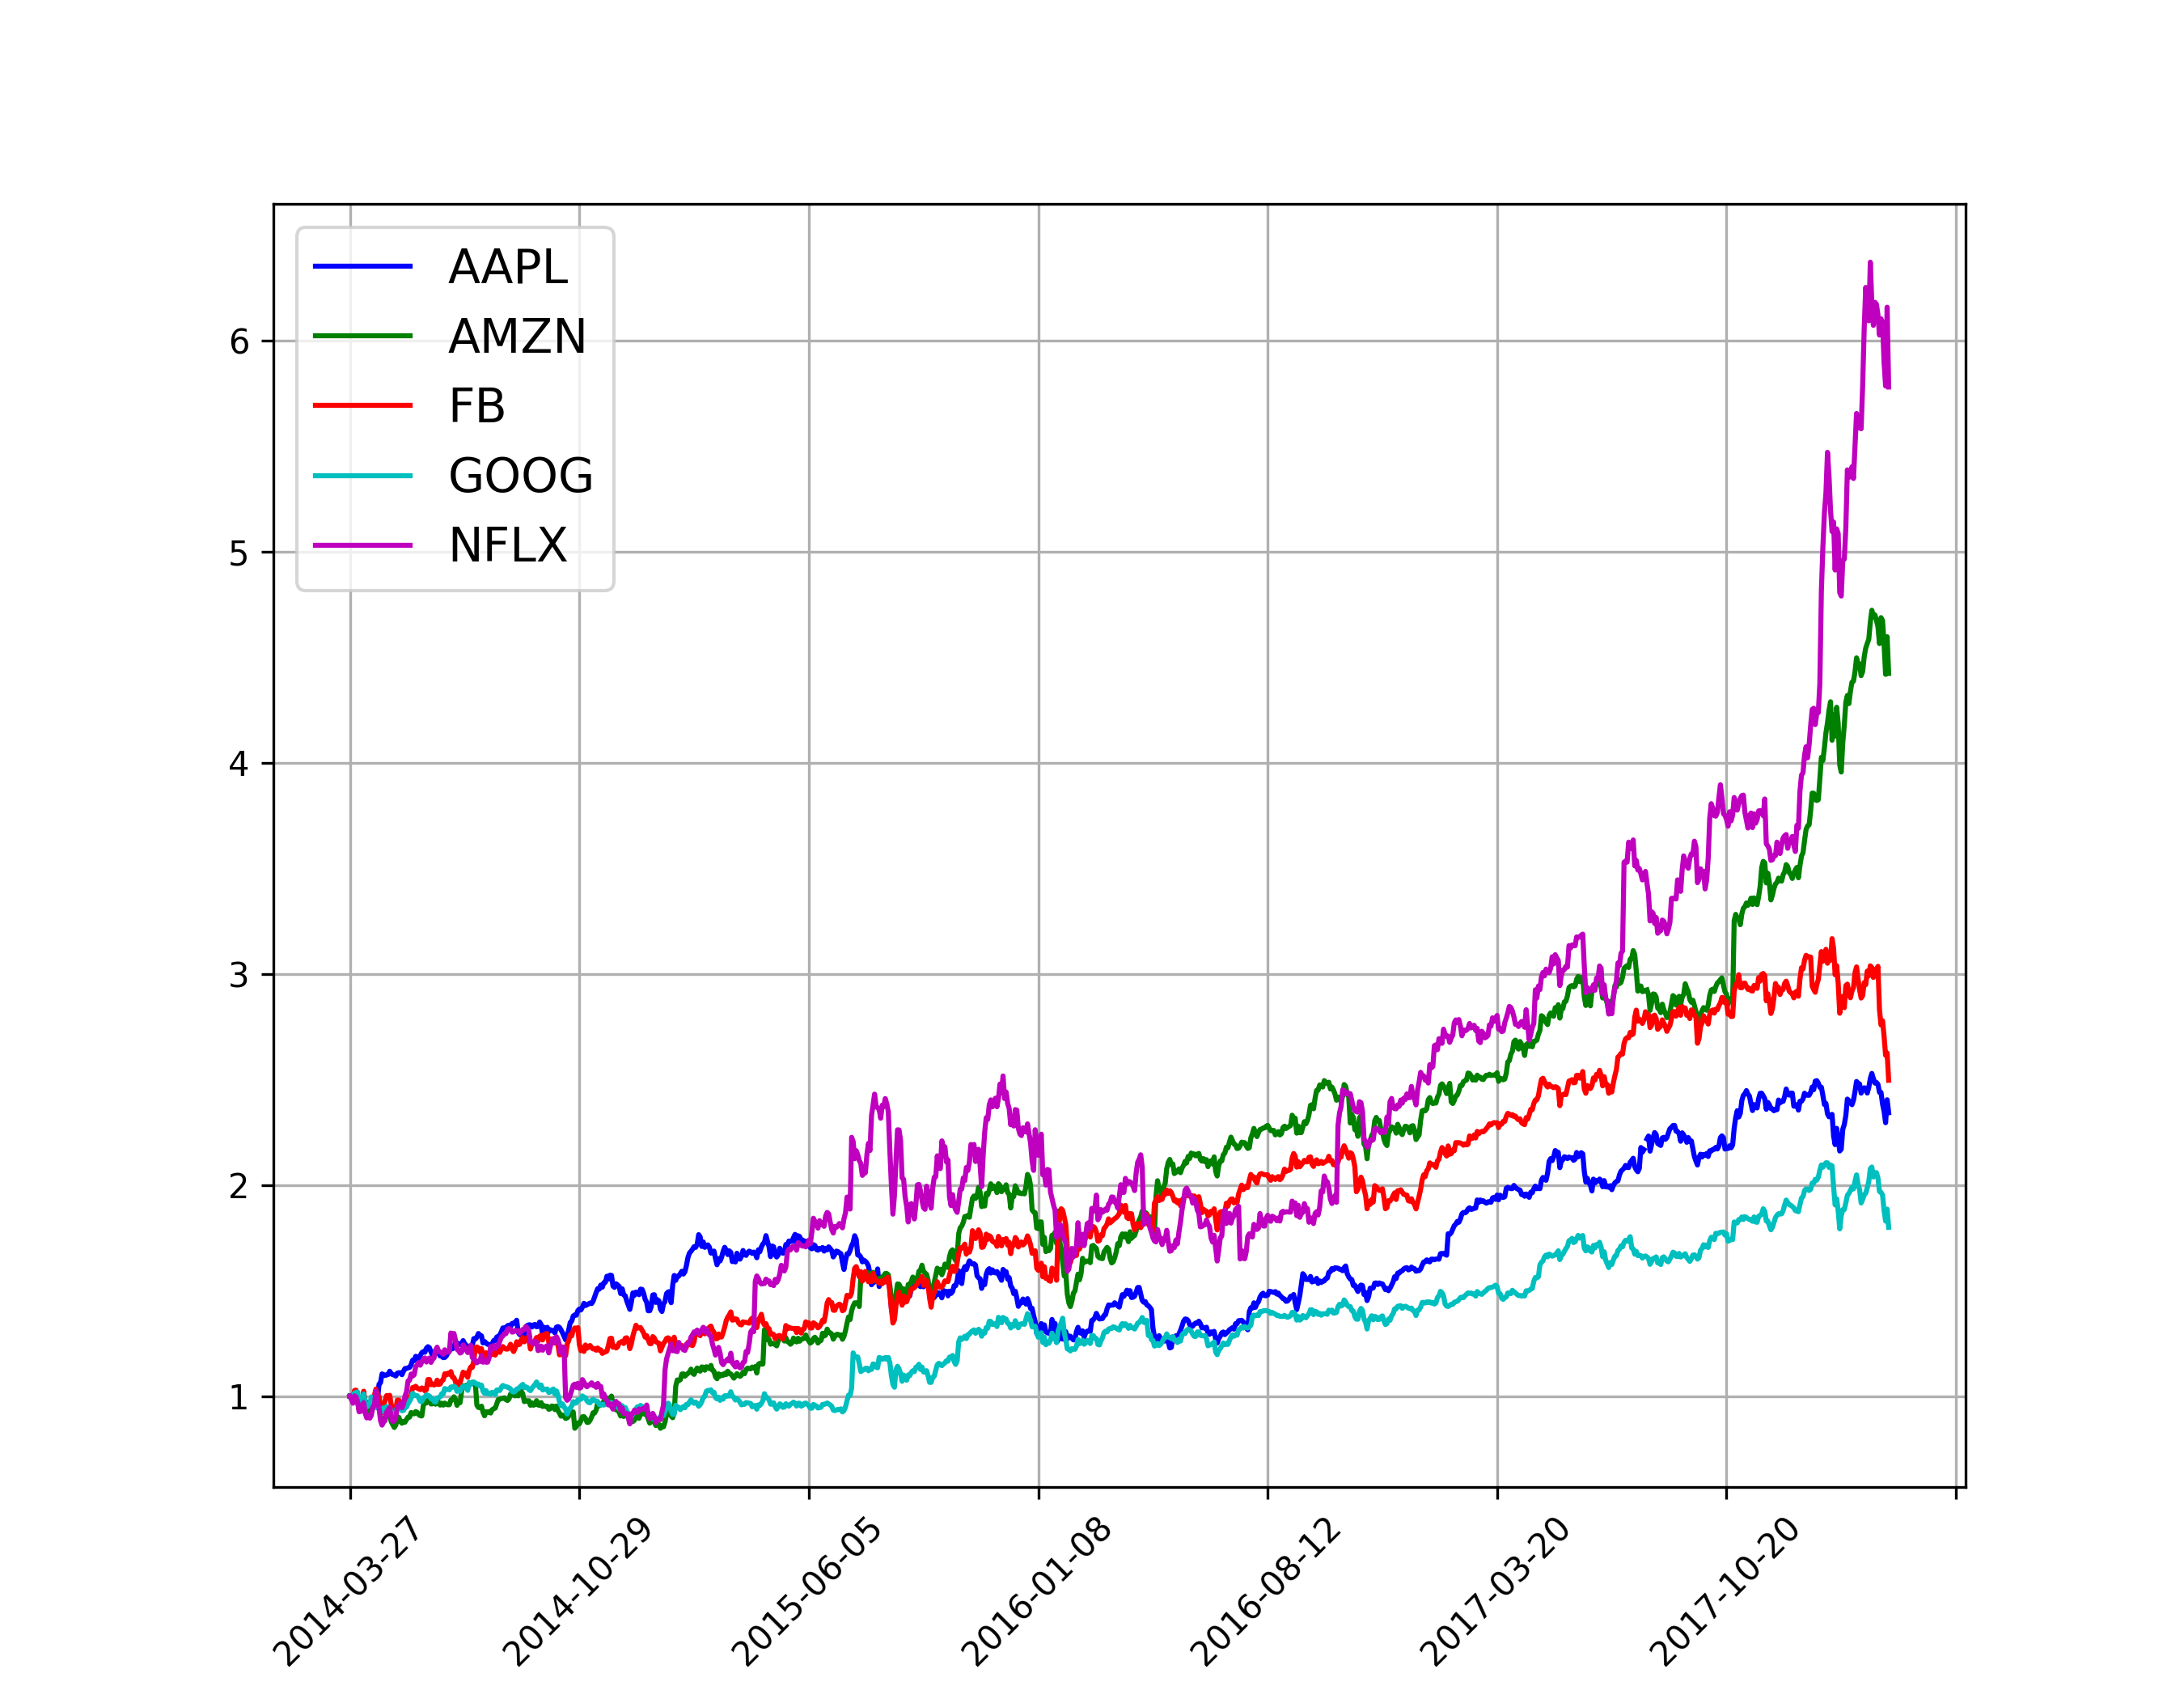
\includegraphics[width=0.7\textwidth]{figures/portfolio_sample}
\caption{Historical series of the closing price of five companies. To compare them, prices have been normalized to the first value in each series}
\label{fig:stocks}
\end{figure}

The correlation of returns across time intervals (called \emph{auto-correlation}) is in general close to zero for most assets. This means that variances can be added across time intervals, hence they will grow with the length of the forecast horizon (while the risk with the square root of the time horizon). Thus, a 5\% annual risk is equivalent to a 2.5\% risk over the first quarter or a 10\% risk over four years.
This can be used to “annualize” risk, i.e. standardize risk numbers to an annual period. The observed daily return standard deviation ($\sigma_{daily}$) can be converted to annual risk according to
\begin{equation}
\sigma_{yearly} = \sigma_{daily}\cdot\sqrt{252}
\end{equation}

These quantities (e.g. daily returns, covariance matrix,\ldots) are easily computed with \texttt{pandas}.

%\subsection{Portfolio Simulation}
%In order to "simulate" a portfolio of $n$ assets it is enough to throw $n$ random weights with the only constraint that they had to sum up to 1.
%In Figure~\ref{fig:mc_portfolio} a large number of simulated portfolios, each made of different proportion of the five assets mentioned above, are shown in a return vs volatility plot.
%Note that in these simulation no attempt of any optimization whatsoever has been made yet.
%
%\begin{figure}[hbtp]
%\centering
%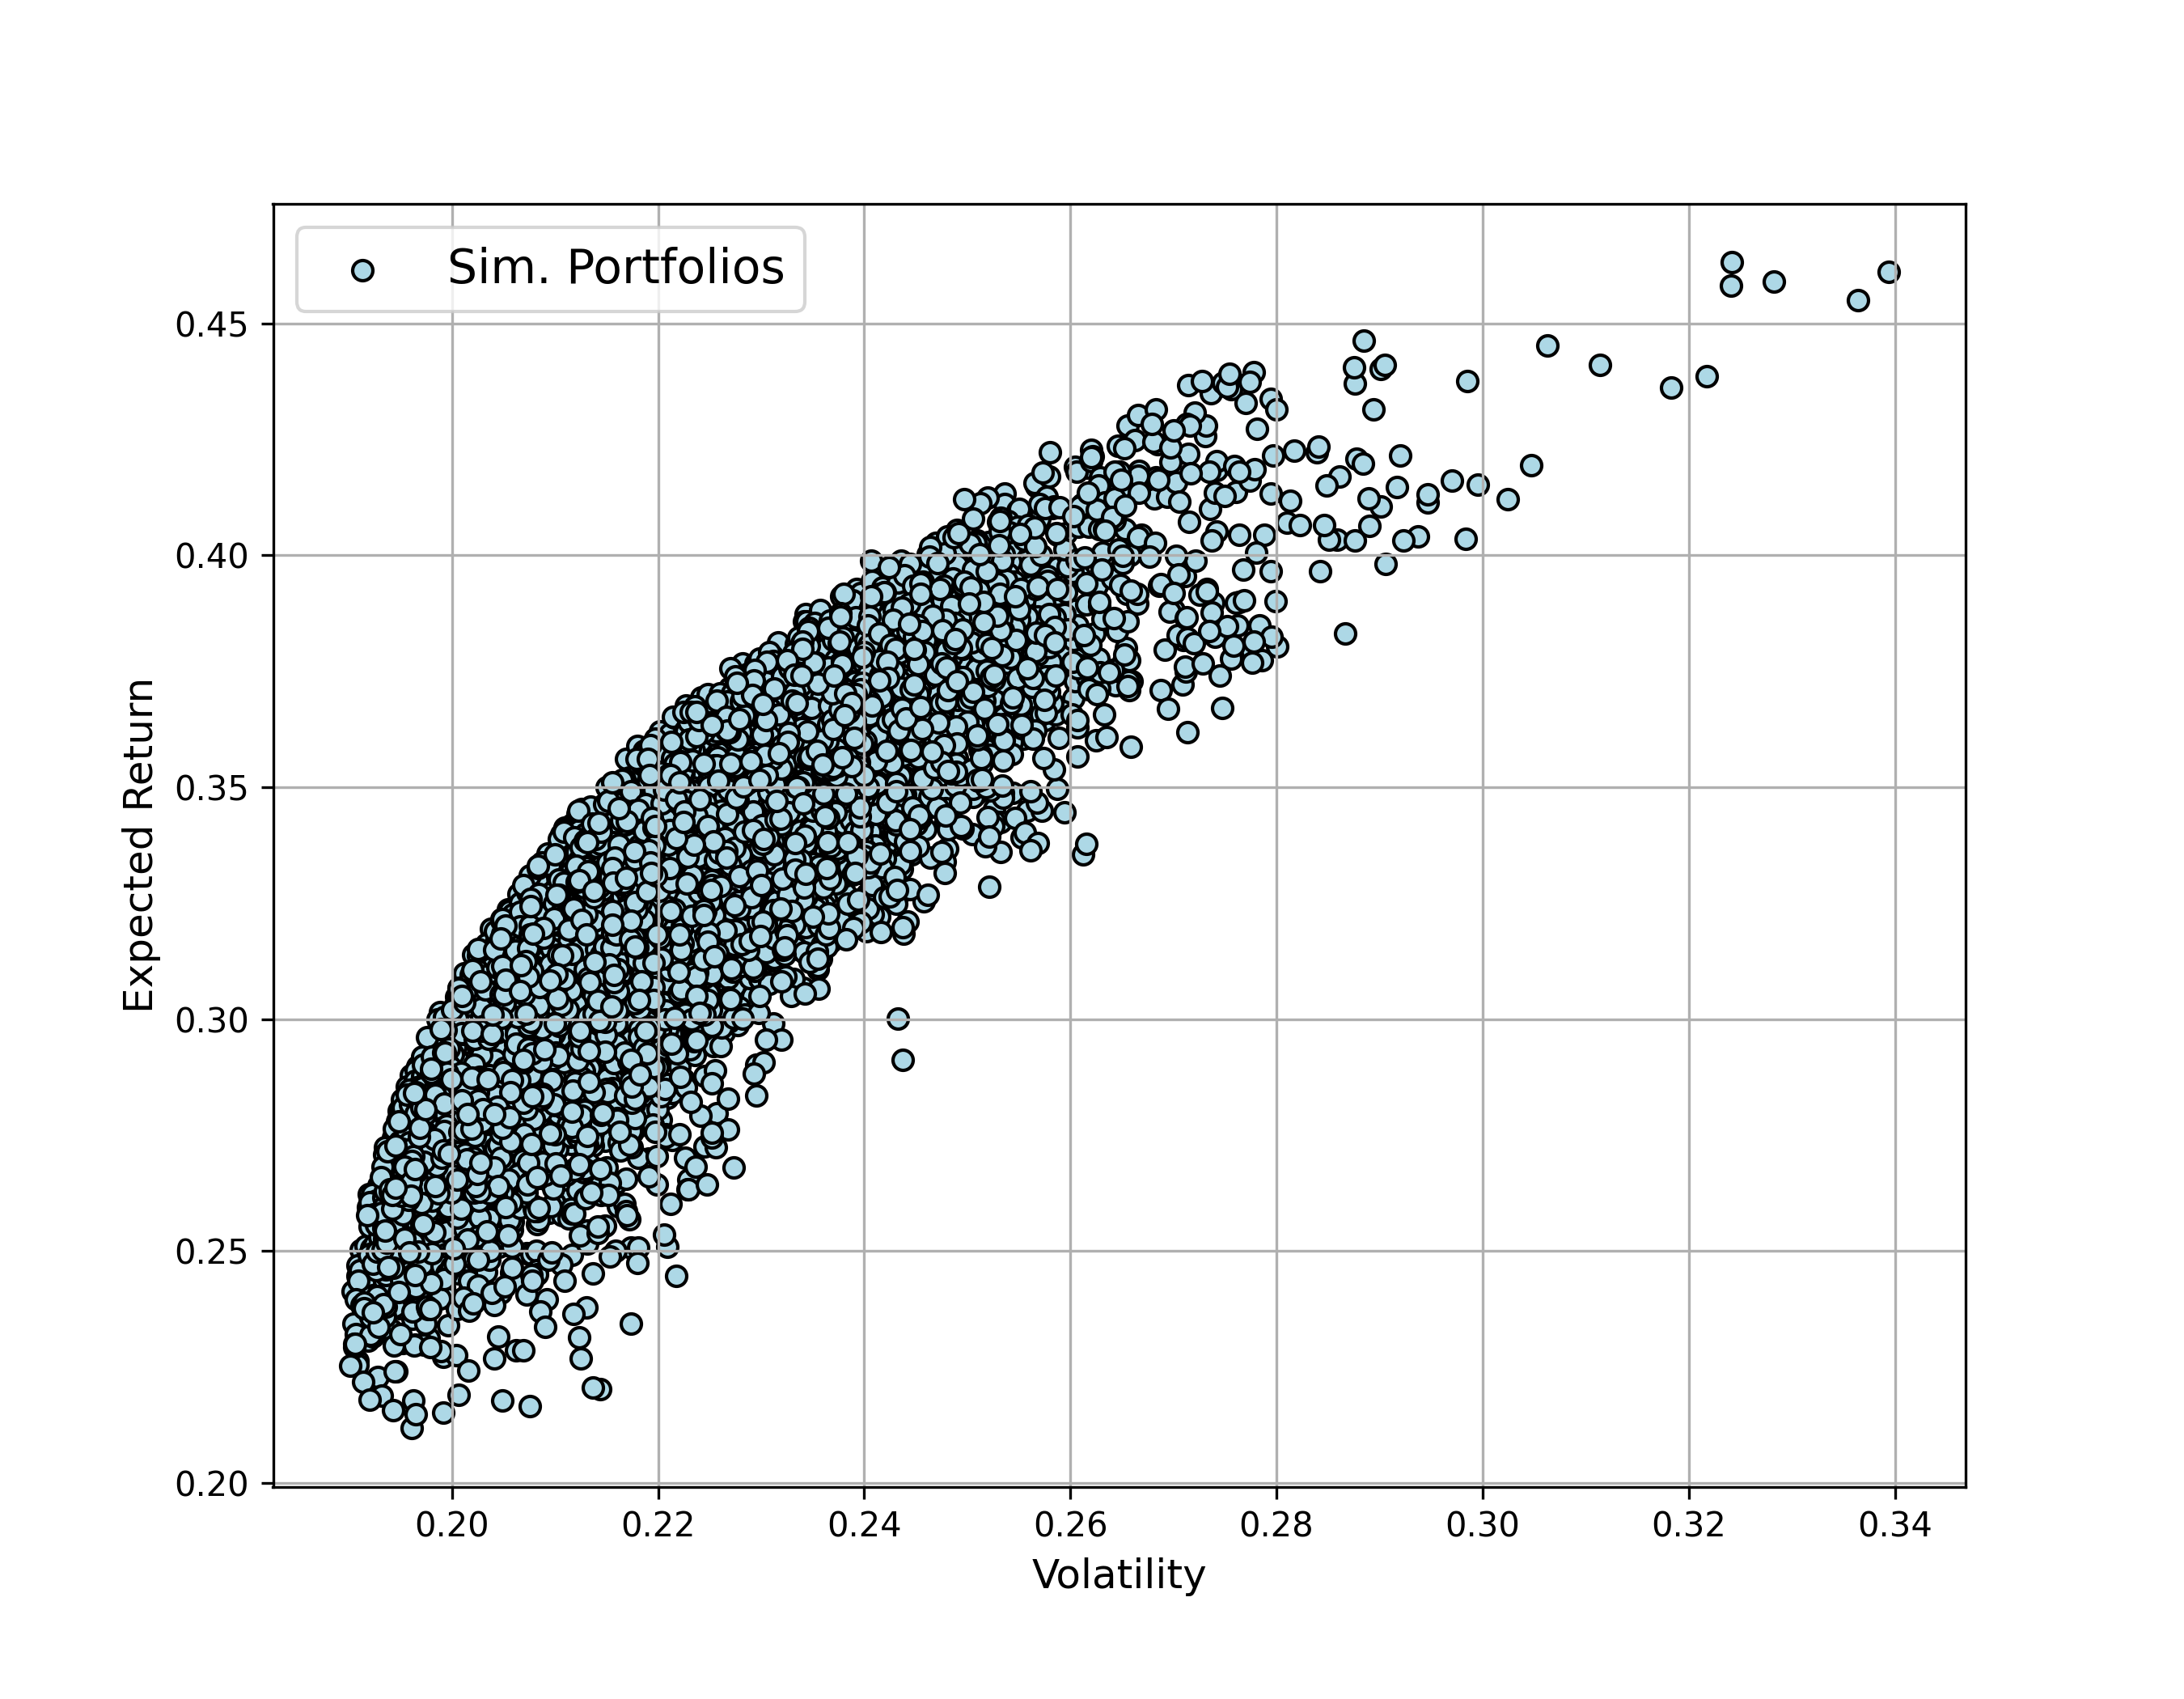
\includegraphics[width=0.7\textwidth]{figures/return_variance}
%\caption{Scatter plot of expected return vs volatility of a large number of simulated portfolios.}
%\label{fig:mc_portfolio}
%\end{figure}
%
%Investors may use \emph{short sales} in their portfolios (a portfolio is short in those stocks with negative weights).
%Although short selling extends the set of possible portfolios we are not going to consider it here.

\subsection{The Model}
\label{optimization}

The Modern Portfolio Theory model states that \textbf{the weights of a portfolio should be chosen such that its volatility (or its variance) is minimized, given a certain level of return}. Alternatively weights can be found by maximizing the return given a certain level of risk.

The application of this model reduces to a minimization problem: given the covariance matrix of the portfolio $\Sigma$, we need to find

\begin{equation}
\underset{\mathbf{w}}{\min}\{\sigma_p^2\} = \underset{\mathbf{w}}{\min}\{\mathbf{w}^T\Sigma\mathbf{w}\}
\end{equation}
with the constraints $\sum_{i}w_i = 1$ , $0 \le w_i \le 1$ and $\mathbf{w}\cdot\mathbf{R}=R_{\textrm{target}}$.

In \texttt{python} we have already seen how to solve minimization problems (see  Section~\ref{sec:minimization-algorithm}) so it is enough to repeat the same steps.
%:
%
%\begin{itemize}
%\tightlist
%\item define an objective function (i.e. the portfolio variance);
%\item define the set of constraints;
%\item set an initial guess for the weights;
%\item run the algorithm with \texttt{scipy.optimize.minimize}.
%\end{itemize}
%
\pythoncodenon{code/portfolios_mpt.py}
\begin{ioutput}
    message: Optimization terminated successfully
    success: True
     status: 0
        fun: 0.19495739520298233
          x: [ 4.342e-01  2.030e-01  1.208e-01  1.796e-01  6.252e-02]
        nit: 6
        jac: [ 1.873e-01  2.208e-01  1.909e-01  1.732e-01  2.350e-01]
       nfev: 36
       njev: 6
multipliers: [ 1.423e-01  2.107e-01]
Expected portfolio return: 0.25
\end{ioutput}

The optimization recommends to devote about 44\% of the portfolio to AAPL, about 10\% to AMZN, 12\% to FB and so on\ldots The expected return is 25\% as desired, with a variance of about 0.036 or, equivalently, a standard deviation of 0.19.

Note that if a \texttt{target\_return} is not specified the algorithm find the \textit{absolute} minimum variance portfolio, the one with the lowest possible risk given the investment universe regardless the portfolio return.

There is no precise way for an investor to determine the “correct” trade off between risk and return. The desired higher expected return needs to be paid for with higher risk. Thus, one is frequently interested in looking at the relative distribution of the two.
In finance terminology, means to trace the \emph{efficient frontier of return and risk}. This can be done by solving the previous minimization for a variety of target returns.

The following example computes the efficient frontier plot (shown in Fig.~\ref{fig:efficient_frontier}) with the return ranging from 0.20 to 0.50.

\pythoncodenon{code/portfolios_efficient_frontier.py}

\begin{figure}[htb]
\centering
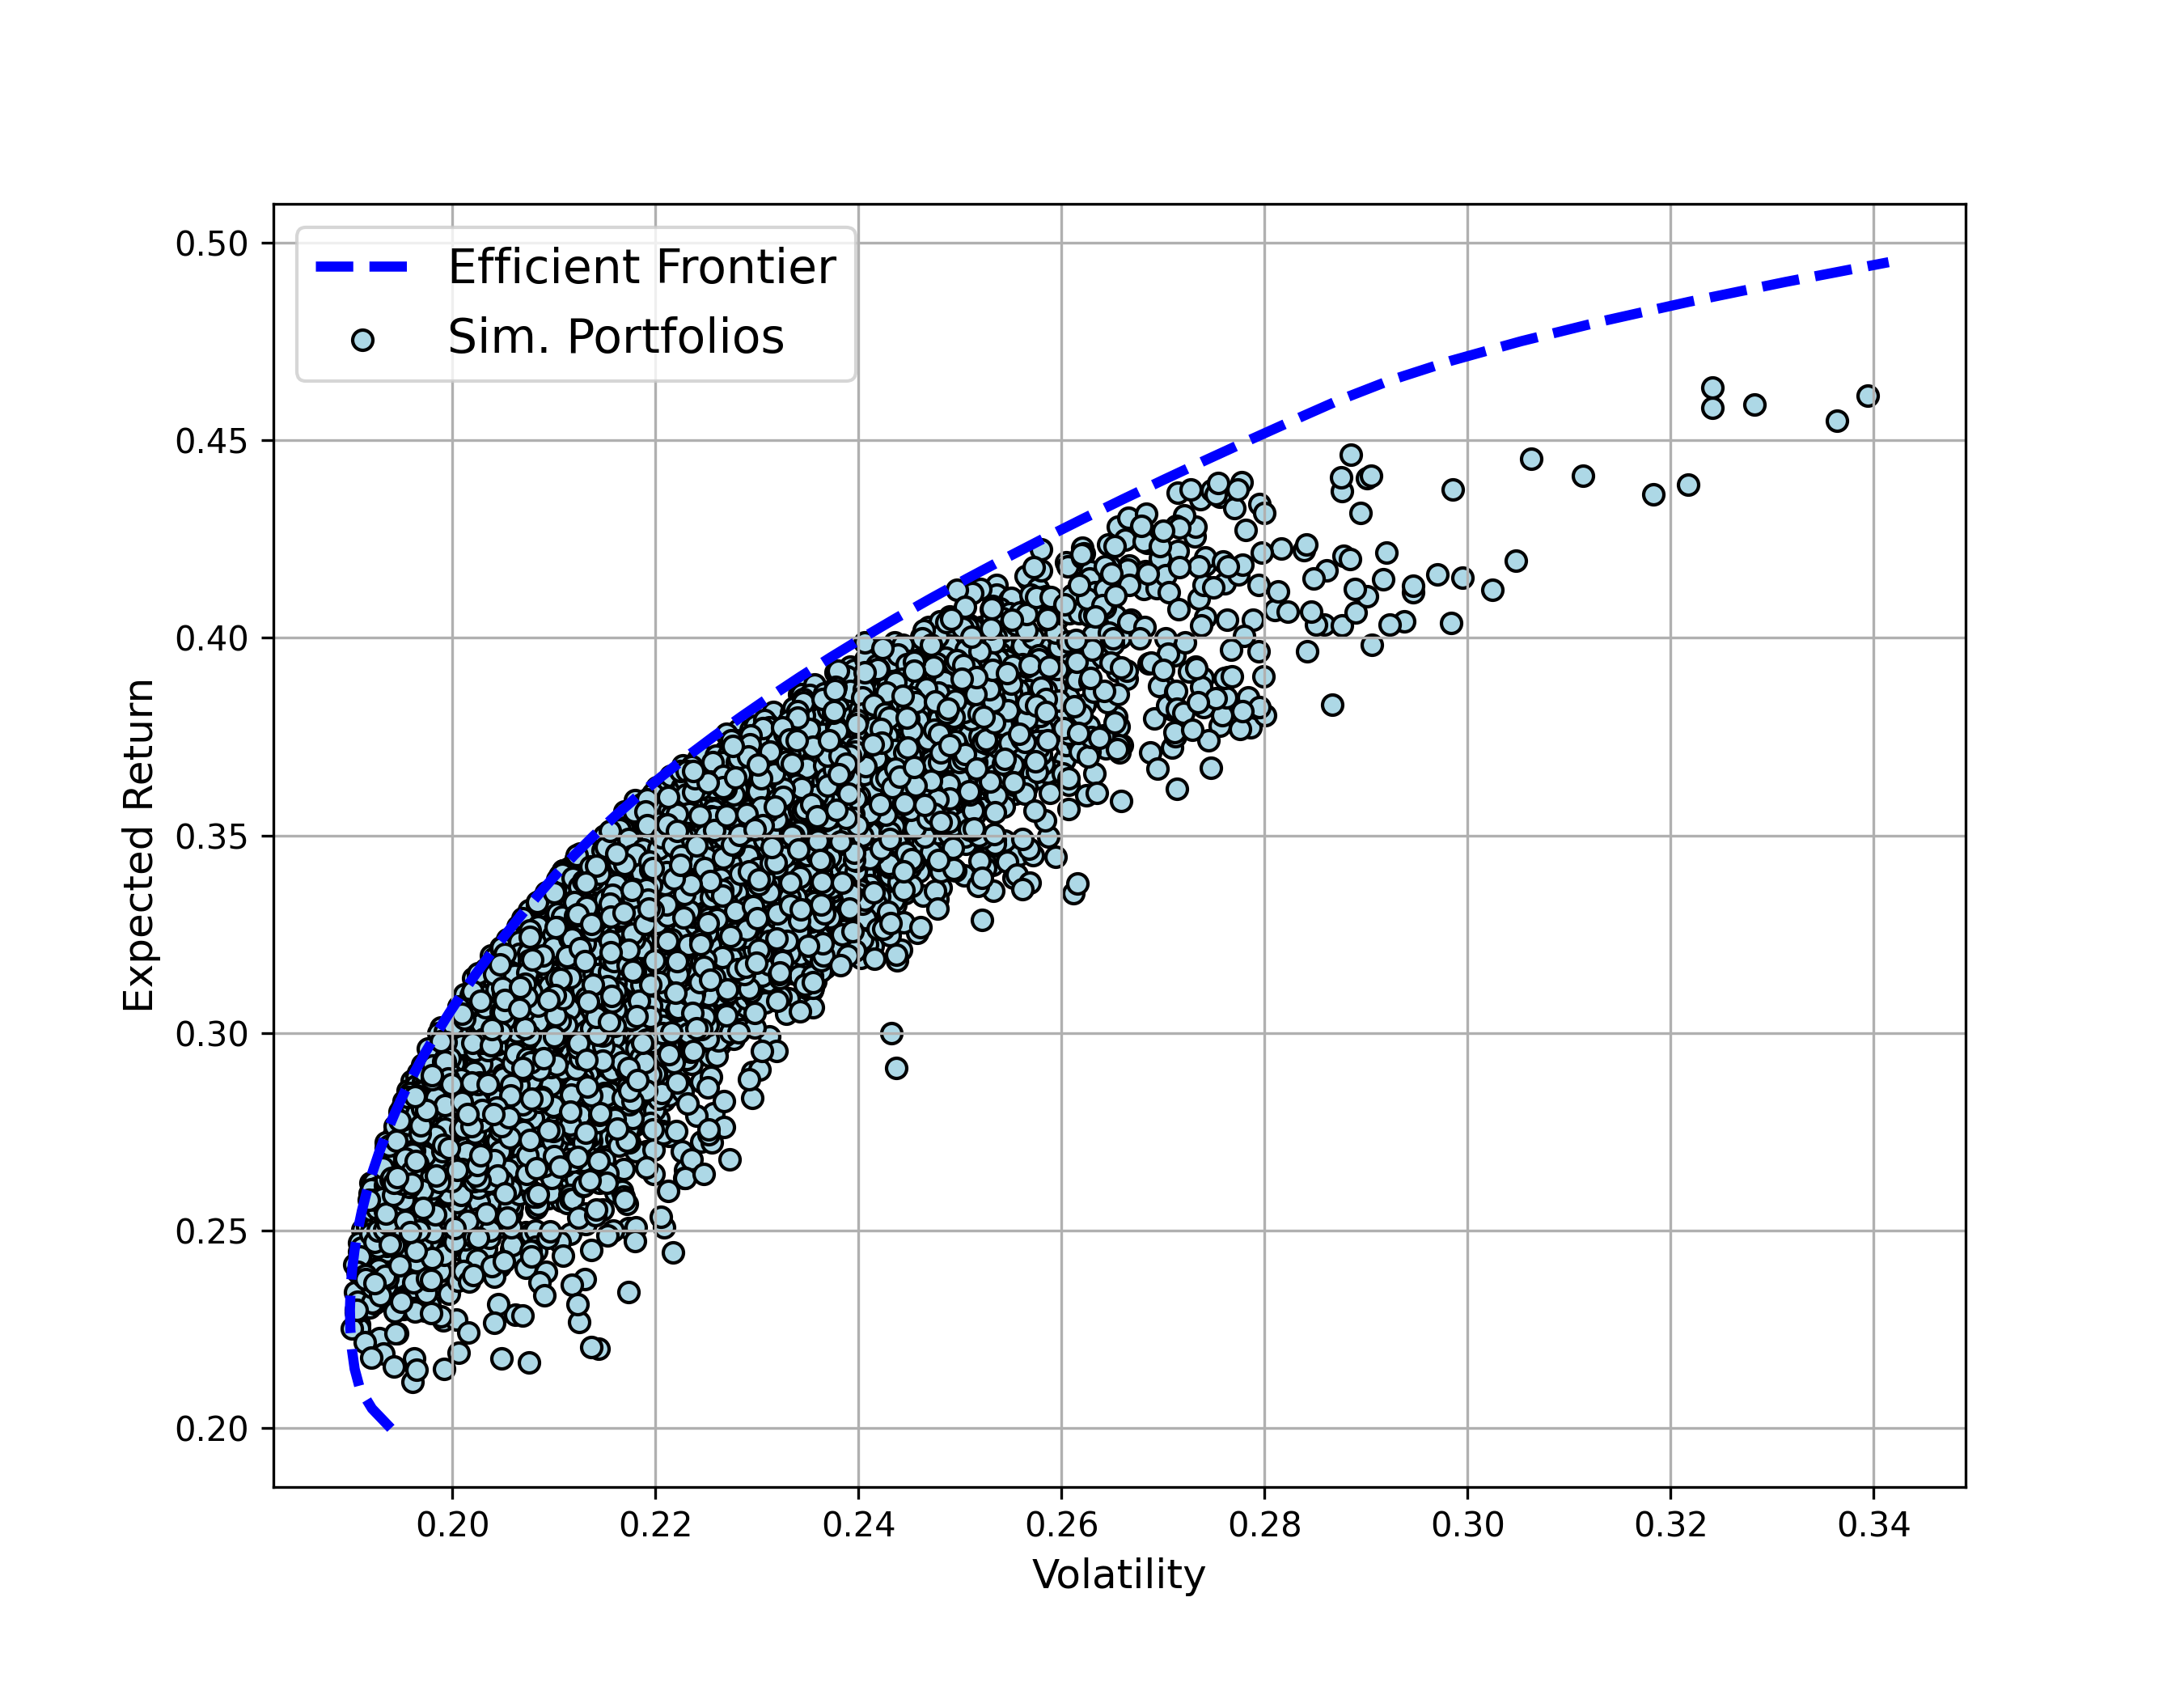
\includegraphics[width=0.7\textwidth]{figures/efficient_frontier}
\caption{Efficient frontier for our example portfolio obtained minimizing the the variance and requiring an expected return between 0.20 and 0.50.}
\label{fig:efficient_frontier}
\end{figure}

\emph{Efficient portfolios} offer investors the highest possible expected return for a given level of risk.
An investor seeking high expected returns and low volatility should invest only in efficient portfolios and will choose from their set based on her risk tolerance.

\subsection{Limits of the Markowitz Model}
\label{sec:limits-of-the-markowitz-model}

Despite the significant utility of the Markowitz theory, there are some major limitations in this model:

\begin{enumerate}
\tightlist
\item the tendency to produce extreme portfolios combining extreme shorts with extreme longs. As a result, portfolio managers generally do not trust these extreme weights. This problem is typically caused by
estimation errors in the mean return vector and covariance matrix;
\item the portfolio weights tend to be extremely sensitive to very small changes in the expected returns. For example, even a small increase in the expected return of just one asset can dramatically alter the optimal composition of the entire portfolio;
\item the presence of heavy tails in the return distributions can result in significant errors in covariance estimates as well.
\end{enumerate}

%Extensions of the Markowitz model are defined in~\cite{bib:post_modern_theory} and~\cite{bib:black_litterman}, although they are beyond the scope of these lectures.

\section{Portfolios with a Risk-Free Asset}
\label{portfolios-with-a-risk-free-asset}

When one of the investments available is a risk-free asset, then the efficient frontier transform to a particularly simple form. The risk–return combinations of the risk-free investment and a risky portfolio lie on a straight line connecting the two investments: the \emph{capital allocation line} (CAL). The slope of the CAL measures the trade off between risk and return: a higher slope means investors receive a higher expected return in exchange for taking on more risk.

The capital allocation line aids investors in choosing how much to invest in a risk-free asset and one or more risky assets.

The simplest example of such kind of portfolios is the one containing only two assets: a risk-free Treasury bill and a stock. Assume that the expected return of the Treasury bill is $\mathbb{E}(R_f)=3\%$ (its risk is 0\%), and that the expected return of the stock is $\mathbb{E}(R_r)=10\%$ and its standard deviation $\sigma_r=20\%$. The question that needs to be answered for any individual investor is how much to invest in each of these assets.

The expected return ($\mathbb{E}(R_p)$) of this portfolio is calculated as follows:

\begin{equation*}
\mathbb{E}(R_p) = \mathbb{E}(R_f)\cdot w_f + \mathbb{E}(R_r)\cdot (1- w_f)
\end{equation*}
where $w_f$ is the relative allocation to the risk-free asset.

The calculation of this portfolio risk is simple because the standard deviation of the Treasury bill is 0\%. Thus

\begin{equation*}
\sigma_p = (1-w_f)\cdot \sigma_r
\end{equation*}
%In this simple example, if an investor invested 100\% into the risk-free asset ($w_f=1$), the expected return would be 3\% and the risk of the portfolio would be 0\%. Otherwise, investing 100\% into the stock ($w_f=0$) would give an investor an expected return of 10\% and a portfolio risk of 20\%. If the investor allocated 25\% to the risk-free asset and 75\% to the risky asset, the portfolio expected return and risk calculations would be
%
%\begin{equation*}
%\begin{gathered}
%\mathbb{E}(R_p) = (3\% \cdot 25\%) + (10\% \cdot 75\%) = 0.75\% + 7.5\% = 8.25\% \\
%\sigma_p = 75\% \cdot 20\% = 15\%
%\end{gathered}
%\end{equation*}
%\noindent
%If you plot these three points they lay on a line.

If we added a risk-free asset, with an expected return of 10\%, to the five risky ones considered so far we could repeat the Markowitz minimization to determine the efficient frontier of the resulting portfolio. We need to update the \texttt{PortfolioOptimizer} class to take into account the new asset, in particular we update the return vector, appending the risk-free return, and the covariance matrix, adding a row and a column with zeros.

\pythoncodenon{code/portfolios_cal.py}

\begin{figure}[htb]
\centering
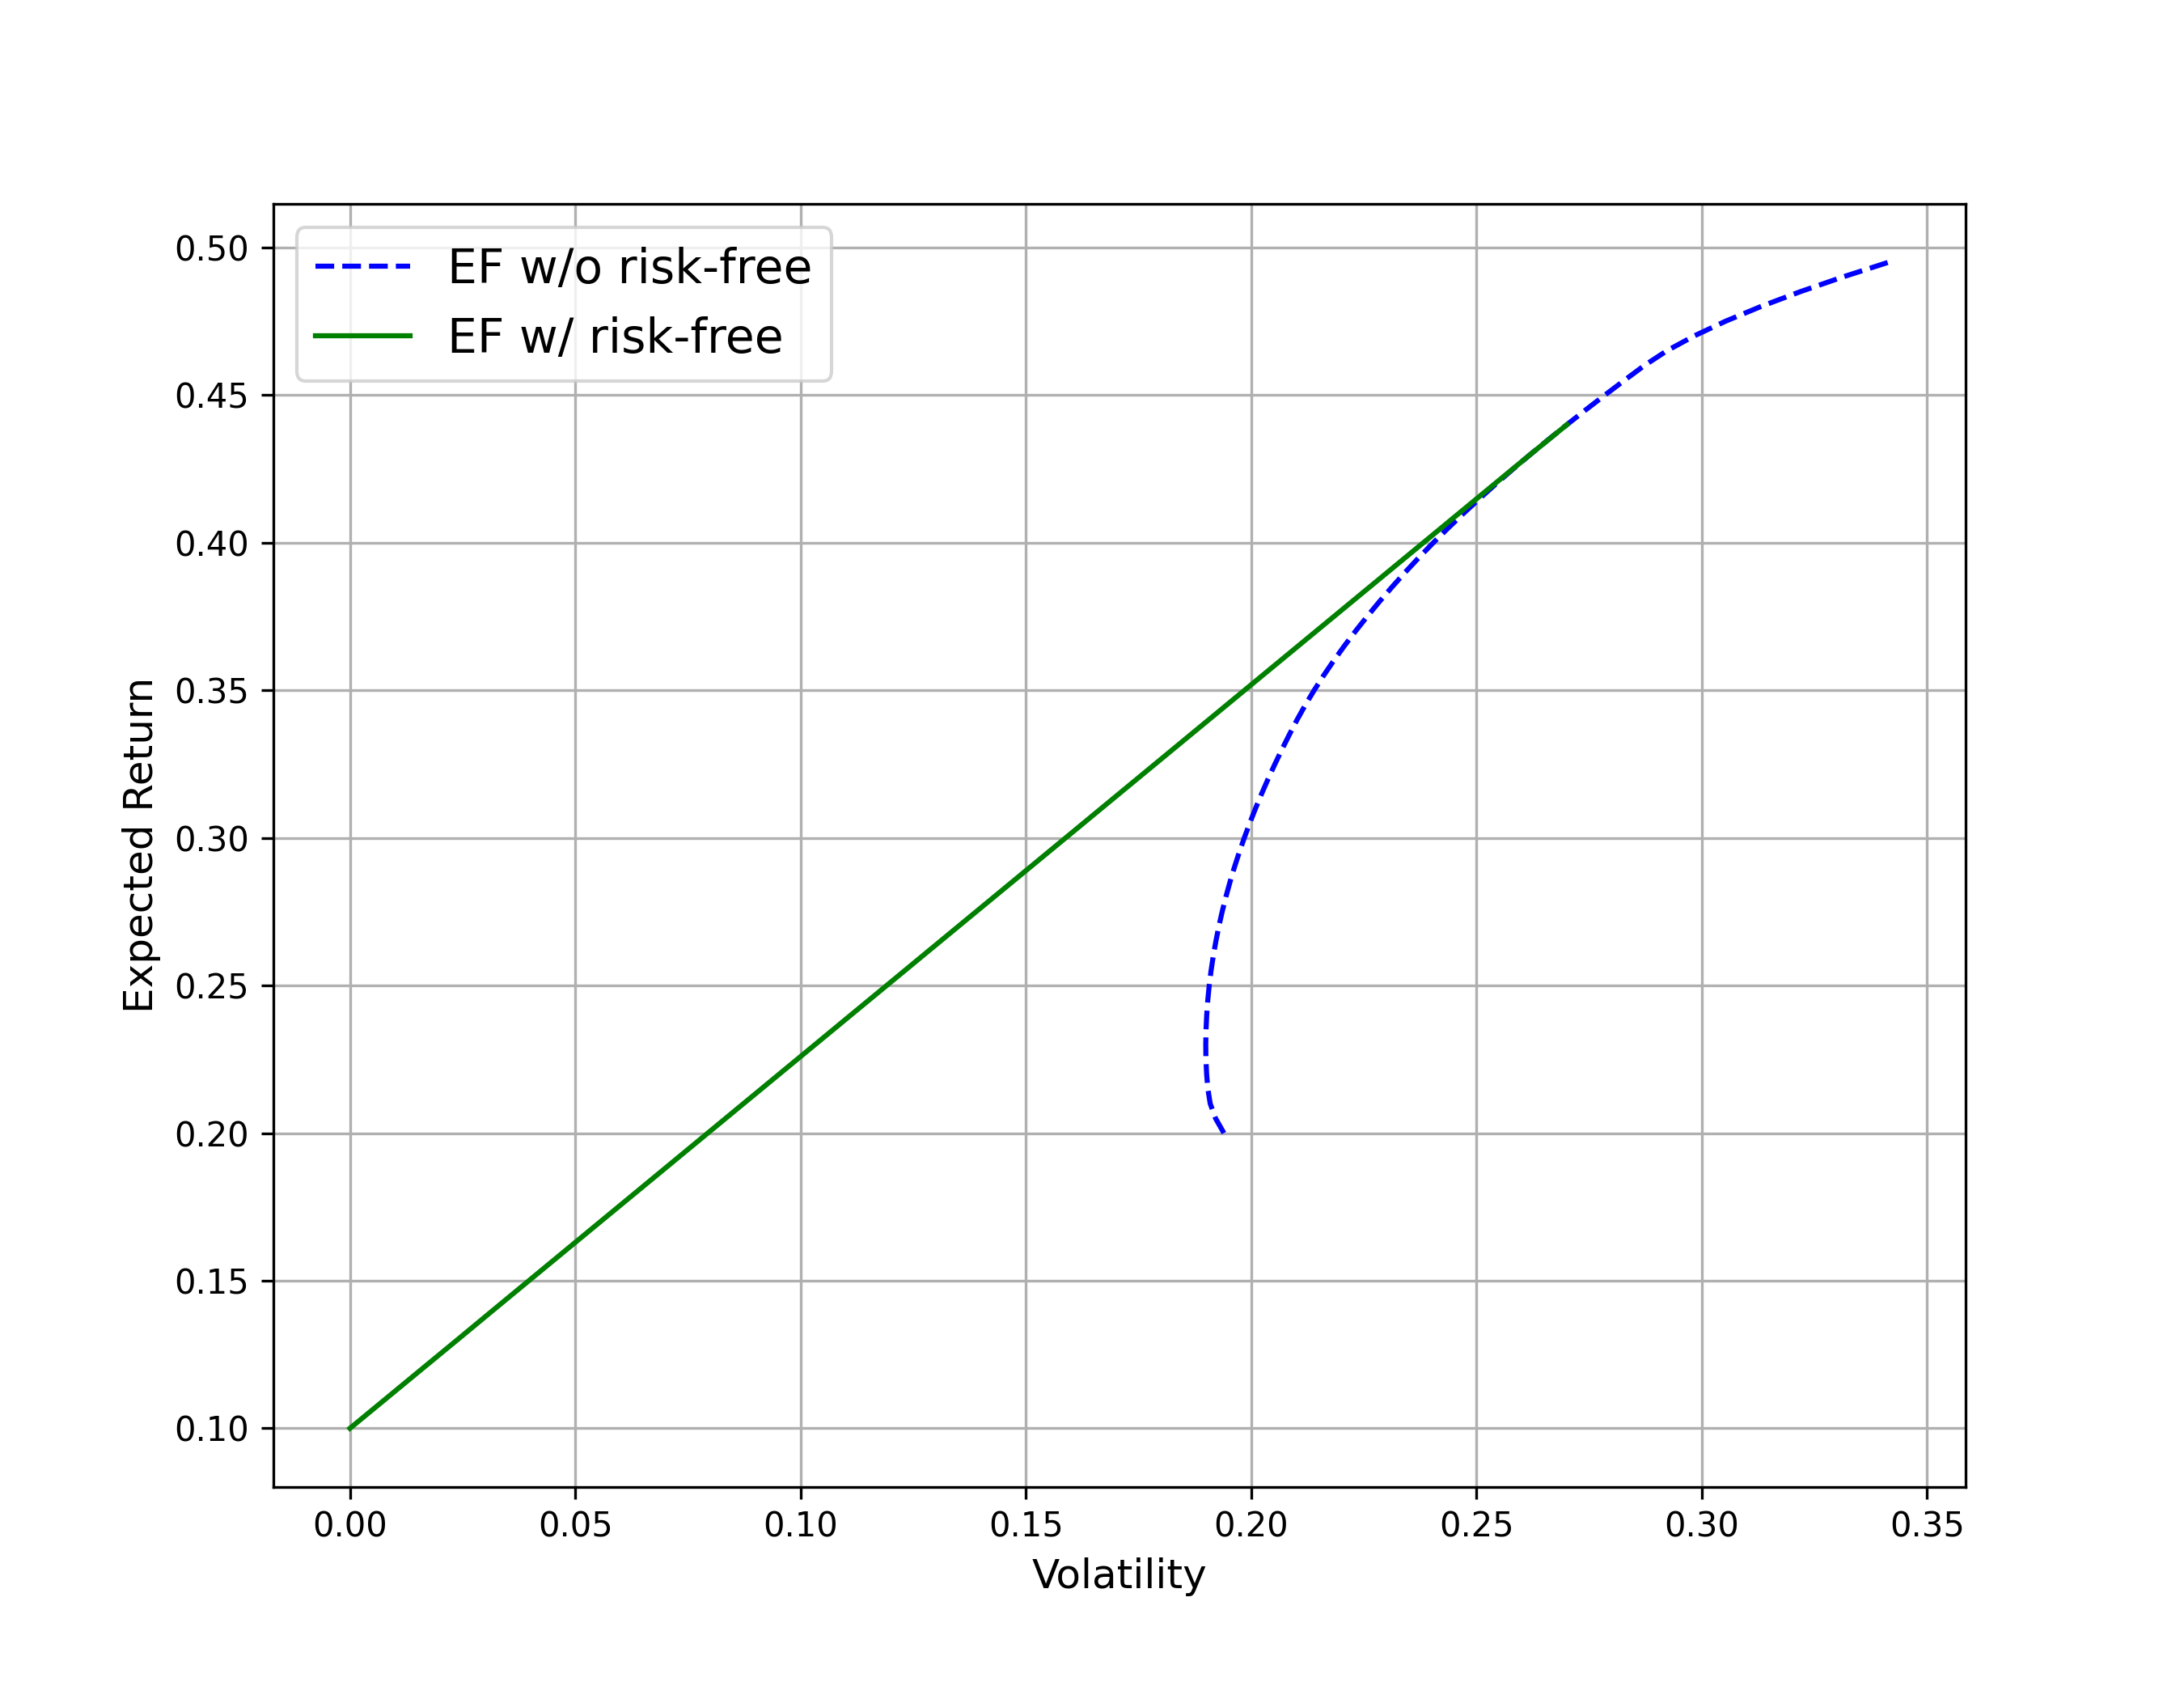
\includegraphics[width=0.7\textwidth]{figures/cal}
\caption{Comparison of efficient frontier with a risk-free asset (red) and with risky asset only (blue).}
\label{fig:cal}
\end{figure}

As expected the efficient frontier has become a straight line, tangent to the frontier of the risky assets (Fig.~\ref{fig:cal}). When the target is 10\% the entire investment is allocated to the risk-free asset, as the target increases the fraction of risky assets grows proportionally to the volatility.

\textit{It is important to notice that in general the relative proportions among the risky investments do not change with or without the risk-free asset. Only the allocation between the risk-free and the risky parts varies.}

\subsection{The Sharpe Ratio}
\label{sec:the-sharpe-ratio}
The goal of an investor who is seeking to earn the highest possible expected return for any level of volatility is to find the portfolio that generates the steepest possible line when combined with the risk-free investment. This line slope is called the \emph{Sharpe ratio} of the portfolio.

For a portfolio of risky assets let be

\begin{itemize}
\tightlist
\item $R_r$ its expected return;
\item $\sigma_r$ its standard deviation in return;
\item $r_f$ the return of a risk-free asset.
\end{itemize}

A plausible single measure of attractiveness of a portfolio (as opposed to the two measures, risk and return, proposed by MPT model) is the Sharpe ratio:

\begin{equation}
\mathcal{S} = \cfrac{R_r - r_f}{\sigma_r}
\end{equation}
\noindent
In words, it measures how much additional return is achieved for the higher risk taken on, relative to investing all in the risk-free asset.

The portfolio that maximizes this ratio has some interesting properties. Suppose that

\begin{itemize}
\tightlist
\item
  $R_\textrm{target}$ the desired target return;
\item
  $w_r$ the fraction of wealth placed in the portfolio (the rest placed in the risk-free asset).
\end{itemize}
\noindent
To meet the target return the weights need to be chosen such that:

\begin{equation*}
(1 - w_r)\cdot r_f + w_r\cdot R_r = R_\textrm{target}
\end{equation*}
\noindent
The standard deviation of the investment is: $w_r\cdot \sigma_r$. Solving for $w_r$ in the equation above, we get:

\begin{equation*}
	w_r = \cfrac{R_\textrm{target} - r_f}{R_r - r_f}
\end{equation*}
Thus, the standard deviation of the portfolio is:

\begin{equation*}
w_r\cdot \sigma_r = \left(\cfrac{R_\textrm{target} - r_f}{R_r - r_f}\right)\cdot \sigma_r
\end{equation*}
Minimizing the portfolio standard deviation means:

\begin{equation}
\textrm{min}\left\{\cfrac{R_\textrm{target} - r_f}{R_r - r_f}\cdot \sigma_r\right\} = \textrm{min}\left[\cfrac{R_\textrm{target} - r_f}{\mathcal{S}}\right]
\end{equation}

Since in the above formula both $R_{\textrm{target}}$ and $r_f$ are constant, the minimization is equivalent to the maximization of the denominator of the expression, hence of the Sharpe ratio $\mathcal{S}$.

\begin{equation}
\textrm{min}\left\{\cfrac{R_\textrm{target} - r_f}{\mathcal{S}}\right\}
\implies\textrm{max}\left\{\cfrac{R_r - r_f}{\sigma_r}\right\}
\end{equation}

So, regardless of investor risk/return preference, \emph{the investment should go in the portfolio that maximizes the Sharpe ratio}, because it will be the one that minimize the risk (i.e. standard deviation) and maximize the return at the same time.

Let's compute the Sharpe portfolio with our sample.

\pythoncodenon{code/portfolios_sharpe.py}

\begin{ioutput}
    message: Optimization terminated successfully
    success: True
     status: 0
        fun: -1.0543579694260374
          x: [ 9.120e-02  6.081e-01  3.437e-17  2.708e-17  3.007e-01 0.000e+00]
        nit: 6
        jac: [-3.780e-01 -3.792e-01 -2.520e-01  1.715e-02 -3.790e-01 nan]
       nfev: 37
       njev: 6
multipliers: [-3.786e-01]
Sharpe ratio: 1.054
\end{ioutput}

Figure~\ref{fig:sharpe_ratio} shows the optimization results. Notice that in general the relative proportions of the stocks are the same as in the previous case (at the same level of return) where we explicitly included a risk free asset.

\begin{figure}[htb]
\centering
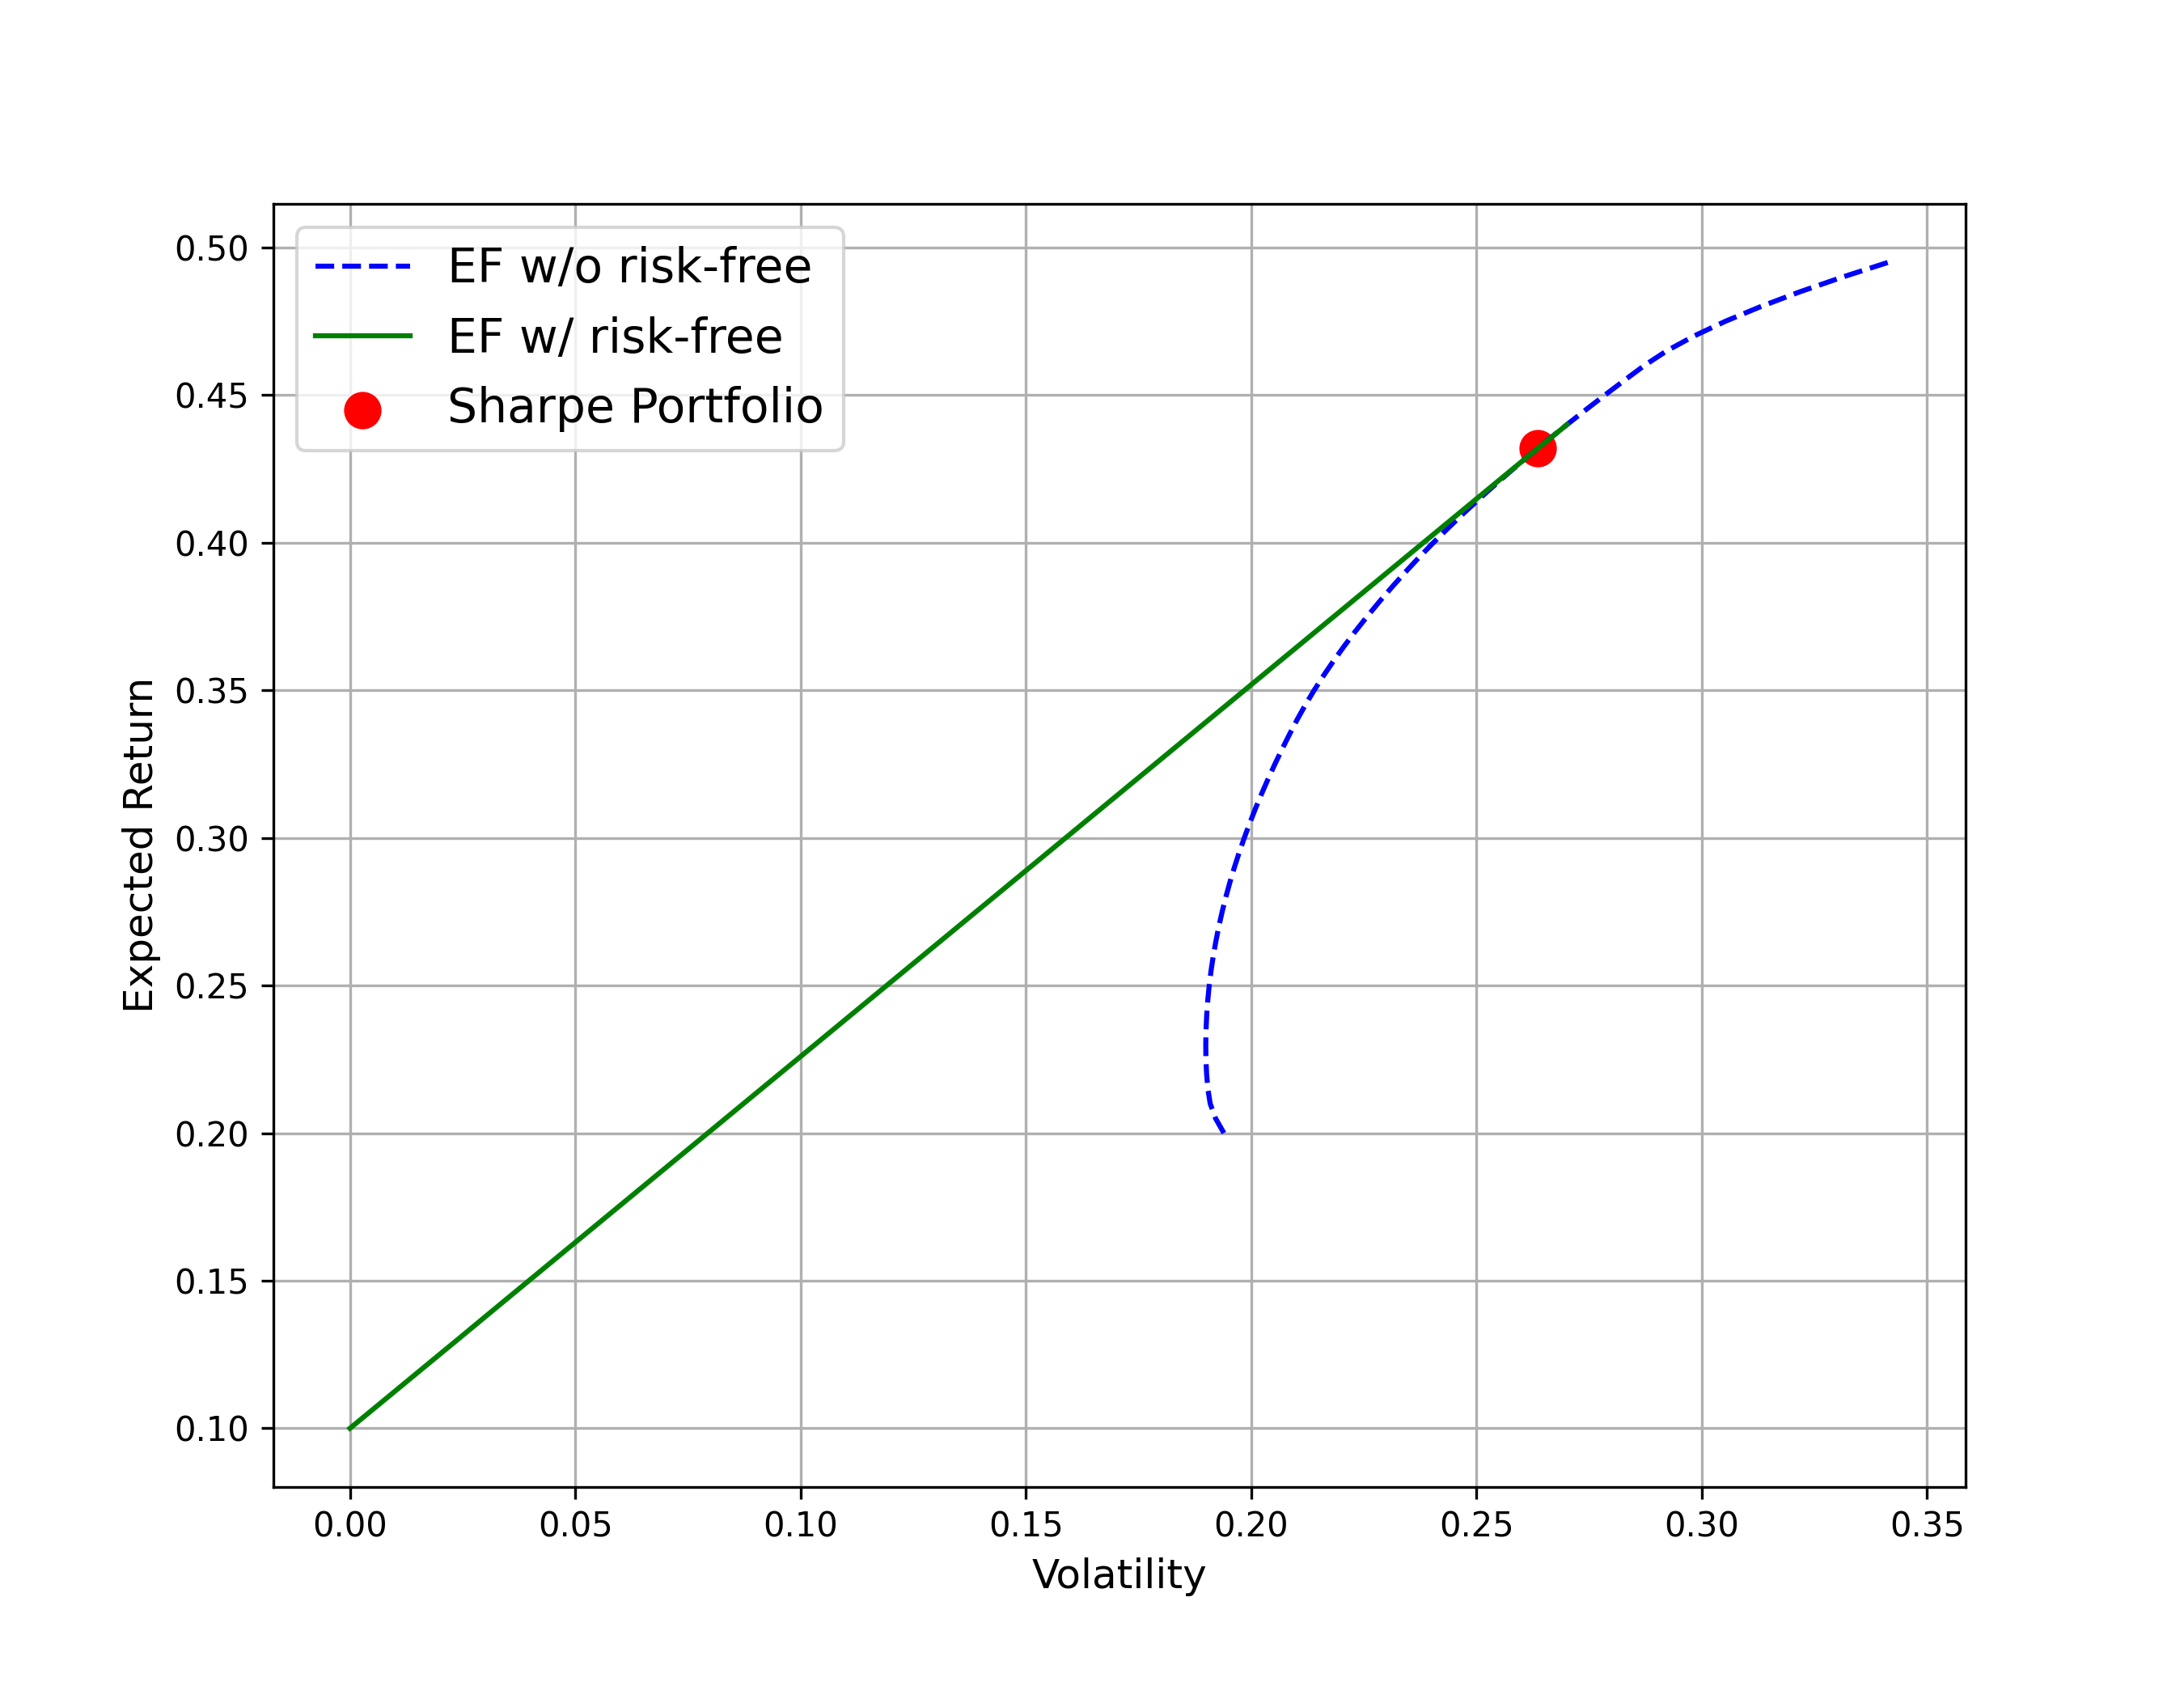
\includegraphics[width=0.7\textwidth]{figures/sharpe_ratio}
\caption{Sharpe portfolio (green cross) compared to the efficient frontier with a risk-free asset (red) and with risky asset only (blue).}
\label{fig:sharpe_ratio}
\end{figure}

So using the Sharpe ratio gives a portfolio that is on the efficient frontier, and gives the maximum return relative to putting all our money in the risk-free asset so is on the CAL too. Graphically it sits in the only place that belongs to both curves: the tangent point.

Usually, any Sharpe ratio greater than 1.0 is considered acceptable to good by investors. A ratio higher than 2.0 is rated as very good. A ratio of 3.0 or higher is considered excellent. A ratio under 1.0 is sub-optimal.

\begin{finmarkets}
As we have seen the goal of Sharpe ratio optimization in asset allocation is to find portfolio weights that maximize the Sharpe ratio, which is:
\begin{equation*}
\text{Sharpe Ratio} = \frac{\text{Expected Portfolio Excess Return}}{\text{Portfolio Volatility}}
\end{equation*}

Maximizing Sharpe ratio under certain assumptions (no leverage constraint, full investment,\ldots) leads to weights proportional to:
\begin{equation}
w^*\propto (\delta\Sigma)^{-1}(\mu-r_f)
\label{eq:linear_algebra_optimization_sharpe}
\end{equation}
where $\mu$ is the expected returns vector, $\Sigma$ the covariance matrix (risk), $\delta$ the risk aversion parameter (higher $\delta$ more risk-averse) and $r_f$ the risk-free rate.

This formula comes from mean-variance optimization where the investor maximizes, see Sec.~\ref{sec:markowitz_utility}:
\begin{equation*}
\text{Utility} = \mu_p - \frac{\delta}{2} \sigma_p^2
\end{equation*}
The first-order condition for this optimization gives indeed Eq.~\ref{eq:linear_algebra_optimization_sharpe}.

Note that after computing raw weights $w^*$, they have to be normalized so that the sum equals 1 (fully invested portfolio).
Without normalization, the weights would only be proportional, not actual allocation percentages.

In \texttt{python} this becomes
\begin{ipythonbox}
import numpy as np

excess_returns = mu - rf
weights_raw = np.linalg.inv(delta * sigma).dot(excess_returns)

weights = weights_raw / np.sum(weights_raw)
\end{ipythonbox}

This algorithm gives an \textbf{uncostrained} solution. If you need to add some constrains instead, e.g. avoid short selling, you have to revert back to quadratic programming with \texttt{scipy.optimize.minimize} as done in the previous Sections.
\end{finmarkets}

%\subsection{Optimal Portfolio with Risk-Free Asset}
%
%In the Markowitz portfolio theory presented, there is an assumption that all of the securities have $\sigma > 0$, which excludes the choice for a risk-free security, such as the treasury bond. Of course most investors would like to include a risk-free component in the portfolio, and an obvious solution is to combine a minimum variance portfolio represented by $(\sigma_B, \mu_B)$ with a risk-free asset represented by $(0, r)$ and the combined portfolio will have its risk-return pair $(x, y) = w_0(0, r) + (1-w_0)(\sigma_B, \mu_B)$.
%By varying $w_0$ we end up all the possible portfolios with their risk-return, see~\ref{fig:cal}.
%
%It is natural to choose the risky portfolio to be on the frontier, and even more specifically, we should choose the portfolio that corresponds to the point on the frontier that leads to the tangent line when we connect it with $(0, r)$. This portfolio is indeed very special and it is sometimes referred to as \emph{the market portfolio} $(\sigma_M, \sigma_M)$.
%The straight line in this case is called the \emph{capital market line} (CML), which is a special case of the capital allocation line (see~\ref{portfolios-with-a-risk-free-asset}) where the risky portfolio is the market portfolio. This combination using $(0, r)$ and $(\sigma_M, \mu_M)$ gives us all the points on the CML and they represent an optimized combination.
%
%To see that the CML represents the optimal combination, just perturb the straight line in both directions and see what will happen. If you move the straight line up, then there is no point within the Markowitz bullet, which means the risky portfolio cannot be constructed. On the other hand, if we move the straight line down, there will be a secant line with the bullet, which gives a set of portfolios that are not on the frontier. That would suggest that this risky portfolio can be improved, therefore it is not optimal. \emph{With these arguments we conclude that the combination with the risky portfolio is the optimal combination}.

\section{Utility Function and Markowitz Model}
\label{sec:markowitz_utility}

An \emph{utility function} $u(x)$ is a function of wealth ($x$) that quantifies the ``happiness'' level of the investor. Typically this function has $u'(x) > 0$ and $u''(x) < 0$. The first condition reflects the simple concept that ``the more I have the happier I am''. The latter instead will be described later on in this Section.

In real life, the future wealth level will be uncertain, so we would use a random variable $X$ as the input of the utility function, leading us to the study of its expectation. First of all, it must be noticed that in general $\mathbb{E}[u(X)] \neq u(\mathbb{E}[X])$.
Since investors care for the utility we should prefer a random variable such that $\mathbb{E}[u(X)]$ is maximized.

%From the Jensen’s inequality we get that $\mathbb{E}[u(X)] < u (\mathbb{E}[X])$. Indeed
Using a simple Taylor expansion around the value $\mathbb{E}[X]$:
\begin{equation*}
u(X) = u (\mathbb{E}[X]) + u'(\mathbb{E}[X]) (X - \mathbb{E}[X]) + \frac{1}{2}u''(\mathbb{E}[X]) (X - \mathbb{E}[X])2 + \ldots
\end{equation*}

If we take the expectation of both sides, assuming $u'' < 0$,
\begin{equation*}
  \begin{aligned}
  \mathbb{E}[u(X)] &= u(\mathbb{E}[X]) + u'(\mathbb{E}[X]) \mathbb{E}[X-\mathbb{E}[X]] + \frac{1}{2}u''(\mathbb{E}[X]) \mathbb{E}(X-\mathbb{E}[X])^2 + \ldots\\
  &= u (\mathbb{E}[X]) + \frac{1}{2}u'' (\mathbb{E}[X]) \var(X) + \ldots < u (\mathbb{E}[X])
  \end{aligned}
\end{equation*}
If we let $X$ to be the realized return of certain investment, the investors’ goal would be to maximize the expected utility, and from the last equation above it seems
that we should maximize the expected value of the return ($\mathbb{E}[X]$) and minimize the variance of the return ($Var(X)$) at the same time. \emph{This is what is contained in Markowitz portfolio theory}.
But this result shows that optimizing the return of the portfolio can be viewed as maximizing the utility for the investor. The
advantage of the utility approach is that now we can use different utility functions for different investors’ preferences, mostly about their preferences towards risk.

\subsection{Exponential Utility}
Assume for example $u(x) = 1-e^{-x}$ and $X$ is a normal random variable. Then we find
\begin{equation*}
  \mathbb{E}[u(X)] = 1-\mathbb{E}[e^{-X}] = 1-e^{-\mathbb{E}[X]+ \frac{1}{2}2\var(X)}
\end{equation*}

Since the exponential is an increasing function, the following are equivalent:
\begin{equation*}
\max \mathbb{E}[u(X)] \equiv \min e^{-\mathbb{E}[X]+ \frac{1}{2}\var(X)} \equiv \min\left[-\mathbb{E}[X] + \frac{1}{2}\var(X)\right] \equiv \max\left[\mathbb{E}[X] - \frac{1}{2}\var(X)\right]
\end{equation*}

\emph{In other words maximising the expectation of the utility is equivalent to the Markowitz optimization}.
This is achieved when the expectation of $X$ is high and the variance of $X$ is low, with some balance. If we modify the exponential term to $e^{-\gamma x}$ with $\gamma > 0$, we can modify the balance bias by choosing the parameter a carefully.

How do we interpret the condition $u''<0$ ? Using the approximation
\begin{equation*}
  \mathbb{E}[u(X)] = u (\mathbb{E}[X]) + \frac{1}{2}u''(\mathbb{E})\var(X)
\end{equation*}
we can summarize the risk preference of the investor via utility functions as follows.
\begin{itemize}
\item if $u'' < 0$, $\mathbb{E}[R^A] > \mathbb{E}[R^B]$ so investor prefers $A$ to $B$, so is \emph{risk-averse};
\item if $u'' = 0$, $\mathbb{E}[R^A] = \mathbb{E}[R^B]$ so investor is indifferent to $A$ and $B$, so is \emph{risk-neutral};
\item if $u'' > 0$, $\mathbb{E}[R^A] < \mathbb{E}[R^B]$ so investor prefers $B$ to $A$, so is \emph{risk-seeking}.
\end{itemize}

\subsection{CRRA Utility}

The Constant Relative Risk Aversion utility function (CRRA) is defined as:
\begin{equation}
\begin{cases}
U(W) = \cfrac{W^{(1-\gamma)}}{1-\gamma}\quad\text{for $\gamma \neq 1$}\\
U(W) = \ln(W)\quad\text{for $\gamma = 1$}
\end{cases}
\end{equation}
where $\gamma$ is the coefficient of relative risk aversion.

Let's try to calculate $\mathbb{E}[U(W)]$ with $W = W_0(1 + R)$ where $R\approx N(\mu, \sigma^2)$.
For $\gamma\neq 1$:
\begin{equation*}
\mathbb{E}[U(W)] = \mathbb{E}\left[\cfrac{(W_0(1 + R))^{(1-\gamma)}}{1-\gamma}\right] = \cfrac{W_0^{(1-\gamma)}}{1-\gamma}\mathbb{E}[(1 + R)^{(1-\gamma)}]
\end{equation*}

The key problem arises here since $\mathbb{E}[(1 + R)^(1-\gamma)]$ does not have a simple closed-form expression in terms of $\mu$ and $\sigma^2$ when $R$ is normally distributed. This is due to the fact that CRRA utility involves raising $(1 + R)$ to a power; this non-linear transformation of a normal random variable is not normally distributed in turn which means that the resulting distribution is not characterized by just mean and variance.

Secondly, and unlike the exponential utility case, we cannot use the moment generating function since the expectation involves fractional moments of a lognormal distribution. If we try to approximate using Taylor expansion around $\mu$:
\begin{equation*}
(1 + R)^{(1-\gamma)} \simeq (1 + \mu)^{(1-\gamma)} + (1-\gamma)(1 + \mu)^{-\gamma}(R-\mu) + [(1-\gamma)(-\gamma)/2](1 + \mu)^{-\gamma-1}(R-\mu)^2
\end{equation*}
This shows that higher-order moments matter, not just mean and variance.

Practical implications are that investors with CRRA utility consider skewness, kurtosis, and higher moments hence: mean-variance optimization is not optimal for CRRA investors, portfolio selection requires consideration of higher moments and risk management strategies based purely on variance may be inadequate,

Note that the only case where CRRA utility leads to mean-variance-like preferences is when returns are very small and we can use a second-order Taylor approximation. However, this is an approximation, not an equivalence.

\subsubsection{Lognormal Wealth}

Assume now that future wealth $W$ follows a lognormal distribution $\ln(W)\approx N(\mu,\sigma^2)$. The expected utility calculation now becomes

\begin{equation*}
\mathbb{E}[U(W)] = \mathbb{E}\left[\frac{W^{(1-\gamma)}}{1-\gamma}\right] = \frac{1}{1-\gamma} \cdot \mathbb{E}[W^{(1-\gamma)}]
\end{equation*}

In this particular case (i.e. lognormal variable,) we can use the formula for its moments $\mathbb{E}[X^k]=\exp(k\mu+(k^2\sigma^2)/2)$, therefore
\begin{equation*}
\mathbb{E}[W^{(1-\gamma)}] = \exp\left((1-\gamma)\mu + \frac{(1-\gamma)^2\sigma^2}{2}\right)
\end{equation*}

This gives us:
\begin{equation*}
\mathbb{E}[U(W)] = \frac{1}{1-\gamma} \cdot \exp\left((1-\gamma)\mu + \frac{(1-\gamma)^2\sigma^2}{2}\right)
\end{equation*}

Let's take the natural log of the utility multiplied by $(1-\gamma)$:
\begin{equation*}
\ln((1-\gamma)\mathbb{E}[U(W)] = (1-\gamma)\mu + \frac{(1-\gamma)^2\sigma^2}{2}
\end{equation*}

We can rearrange this into a form similar to mean-variance utility:
\begin{equation*}
\ln((1-\gamma)\mathbb{E}[U(W)] = (1-\gamma)\left[\mu + \frac{(1-\gamma)}{2}\sigma^2\right]
\end{equation*}

which shows that this is equivalent to maximizing:
\begin{equation*}
V(\mu, \sigma^2) = \mu + \frac{(1-\gamma)}{2}\sigma^2
\end{equation*}

In the special case where $\gamma=1$
\begin{align*}
U(W) &= \ln(W) \\
\mathbb{E}[\ln(W)] &= \mu - \frac{\sigma^2}{2}
\end{align*}
which is exactly the mean-variance form.

In conclusion with lognormal wealth and the expectation of the CRRA utility can be expressed as a function of only $\mu$ and $\sigma^2$ and the risk adjustment depends on relative risk aversion $\gamma$.

In this case mean-variance optimization with adjusted risk parameter can be used (risk adjustment depends on investor's relative risk aversion). The asset allocation is valid for longer investment horizons where lognormal returns are more plausible.

\section{Covariance Matrix Denoising}

The question of building reliable estimators of covariance has a long history in finance. The problem comes from the high dimensionality of these matrices; when the size of the time series $T$ is very large, each of the coefficients of the covariance/correlation matrix can be estimated with negligible error (if is assumed not to vary with time). But if $N$ is also large and of the order of $T$, as is often the case in finance, the large number of noisy variables creates important systematic errors in the computation of the inverse of the matrix, which is a direct input of Markowitz’s optimisation formula. These systematic errors lead to sub-optimal portfolios with grossly underestimated out-of-sample risk.

In the following we consider a universe made of $N$ different financial assets that we observe at (say) the daily frequency, defining a vector of returns $r_t$. Since we focus specifically on correlations and not on volatilities, we standardise these returns as follows: we remove the sample mean of each asset; we normalise each return by an estimate $\hat{\sigma}_{it}$ of its daily volatility (for simplicity we use the cross-sectional daily volatility $\hat{\sigma}_{it}=\sqrt{\sum_j r_{jt}^2}$ to remove a substantial amount of non-stationarity in the volatilities, although other possible choices are available like Garch or Figarch models, or simply implied volatilities from option markets). The final standardised return matrix $X = \tilde{r}_{it}/\sigma_i$ where $\sigma_i$ is the sample estimator of the volatility of $\tilde{r}_{it}$, which is now, to a first approximation, stationary.

The most common estimator of the \emph{true} underlying correlation matrix (that we henceforth denote by $[C]$) is to use the sample estimator:
\begin{equation}
[E] = \cfrac{1}{T}[X][X]^{T} = \sum_{k=1}^{N} \lambda_k u_k u_k^{T}
\end{equation}
for the eigenvalues $\lambda_i$ and the associated eigenvectors $u_i$ (see~\ref{sec:eigenvectors-and-eigenvalues}). When $q=N/T\rightarrow 0$, i.e. when the data set is very long, one expects that $[E]\rightarrow [C]$, whereas important distortions survive when $q=O(1)$, even if $T\rightarrow \infty$. In fact, it can be showed that the spectrum of $[E]$ is a broadened version of that of $[C]$, with an explicit $q$-dependent formula relating the two. The distorsion is caused by the \emph{noise} included in the measurement, in particular small $\lambda_i$ are too small and large $\lambda_i$ s are too large compared to the true eigenvalues $[C]$. Thus, recalling that Markowitz’s optimal strategy overweight low variance modes, we understand why using the sample estimator $[E]$ can lead to disastrous results, and why some cleaning procedure should be applied to $[E]$ before any application to portfolio construction.

%The noise masks the actual correlation between the asset returns leading to wrong estimate and consequently to bad portfolio weights.
%Various techniques have been devised in order to eliminate (or at least reduce) the noise and extract a better estimate of the correlation from market data.
\subsection{Mar\v{c}enko-Pastur Technique}
According to the studies of Mar\v{c}enko and Pastur the eigenvalues of the covariance matrix follow the \emph{Mar\v{c}enko-Pastur distribution} which describes the eigenvalues density of a random matrix. The main parameter of the distribution is ratio $q=T/N$ where $T$ is the length of the time-series used to derived the covariance matrix and $N$ the number of variables (assets in our case).

The eigenvalue density ranges between:
\begin{equation}
\lambda_{-} = \sigma^2 \left( 1 - \sqrt{q} \right)^2 \quad \text{and} \quad \lambda_{+} = \sigma^2 \left( 1 + \sqrt{q} \right)^2
\label{eq:marcenko-pastur-distro}
\end{equation}
where $\sigma^2$ is the variance in presence of white-noise i.e. under ideal conditions.

In order to \emph{denoise} the covariance matrix we need to:
\begin{enumerate}
\item compute eigenvalues and eigenvectors of empirical covariance matrix;
\item filter eigenvalues to keep only those above $\lambda_+$, since they are considered real signal, the others are noise;
\item rebuild covariance matrix using only filtered eigenvalues.
\end{enumerate}

This technique allows to reduce covariance matrix noise, improving the parameter estimate accuracy. It is well suited when we are in presence of overfitting i.e. when the number of observations is relatively small compared to the number of variables.
Note that the Mar\v{c}enko and Pastur results do not require multivariate normality of the returns, which then can have fat-tailed distributions.

Below a simple implementation of the described procedure, Fig.~\ref{fig:marcenko_pastur} reports a comparison between original and denoised eigenvalues. Correctly since the original matrix was produced with uncorrelated data all the eigenvalues have been discarded.

\pythoncodenon{code/portfolios_marcenko_pastur.py}

\begin{figure}[htb]
\centering
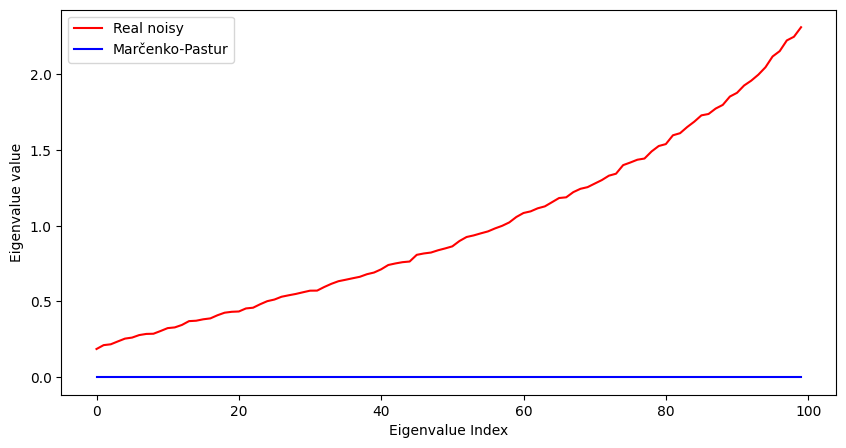
\includegraphics[width=0.7\textwidth]{figures/marcenko_pastur}
\caption{Comparison of the original vs denoised eigenvalues using Mar\v{c}enko-Pastur denoising technique.}
\label{fig:marcenko_pastur}
\end{figure}

\subsection{Rotationally Invariant, Optimal Shrinkage}
This method was first proposed by Ledoit \& Péché (2011) to overcome the issues of another technique called \emph{Eigenvalues substitution}.
For large $N$, the \emph{optimal rotational invariant} (RIE) of $[C]$ reads:
\begin{equation}
\Xi^{RIE} = \sum_{k=1}^N \xi_k^{RIE}u_k u_k^T
\end{equation}
with
\begin{equation}
\xi^{RIE} = \cfrac{\lambda_k}{(1-q+qz_ks_k(z_k))^2}
\label{eq:rie_eigenvalues}
\end{equation}
where $s(z)=N^{-1}\text{tr}(z[I_N]-[E])^{-1}$ and $z_k=\lambda_k - i\eta$.

The rotational invariant hypothesis on an estimator $\Xi$ assumes that one does not have any prior knowledge of the structure of the true eigenvectors, and therefore that the best one can do is to keep the eigenvectors $u_i$ of $[E]$ untouched.

For practical applications, however, Eq.~\ref{eq:rie_eigenvalues} contains the parameter $\eta$ that must be chosen to be small, but at the same time such that $N\eta \gg 1$. A good trade-off is to set $\eta = N^{-1/2}$. Unfortunately, in cases where $N$ is not extremely large (say $N = 400$), this corresponds to $\eta = 0.05$, which is not very small, and this induces a systematic downward bias in the estimator of small
eigenvalues. This bias can be explicitly calculated in simple cases and suggests the following heuristic correction for any $k$:
\begin{equation}
\hat{\xi}_k = \xi^{RIE}_k \cdot \max(1, \Gamma_k)
\end{equation}

Note that $\hat{\xi}_k$ is always greater than or equal to $\xi^{RIE}_k$: this allows one to correct nearly perfectly a systematic
downward bias in the trace of the RIE correlation matrix $\Xi^{RIE}$.

The complete procedure to construct the optimal estimator for $[E]$ reads as this: given the eigenvalues $\lambda_k$ of the sample correlation matrix $[E]$ and $q=N/T$, we define the complex variable $z_k =\lambda_k-i\sqrt{N}$ for any $k$, then

\begin{enumerate}
\item compute for any $k\in[1,N]$:
\begin{equation}
\xi^{RIE}_k=\cfrac{\lambda_k}{(1q+qz_ks_k(z_k))^2}
\end{equation}
with:
\begin{equation}
s_k(z_k)=\cfrac{1}{N}\sum_{j=1;j\neq k}^{N}\cfrac{1}{z_k-\lambda_j}
\end{equation}
\item evaluate at the same time for any $k$
\begin{equation}
\Gamma_k=\sigma^2\cfrac{(1-q+q z_k g_{mp}(z_k))^2}{\lambda_k}
\end{equation}
where
\begin{equation}
g_{mp}(z) = \cfrac{z+\sigma^2(q-1)-\sqrt{z-\lambda_N}\sqrt{z-\lambda_+}}{2qz\sigma^2}
\end{equation}
with:
\begin{equation}
\lambda_+ = \lambda_N\left(\cfrac{1+\sqrt{q}}{1-\sqrt{q}}\right)^2,\quad\quad\sigma^2=\cfrac{\lambda_N}{(1-\sqrt{q})^2}
\end{equation}
where $\lambda_N$ is the smallest empirical eigenvalue;
\item the debiased optimal RIE for any $k$ is
\begin{equation}
\hat{\xi}_k =
\begin{cases}
\Gamma_k\xi^{RIE}_k\quad\text{if }\Gamma_k>1\\ \\
\xi^{RIE}_k\quad\text{otherwise}
\end{cases}
\end{equation}
\end{enumerate}

\section{Portfolio Diversification}

A security total risk can be divided into \emph{unsystematic}, the risk portion peculiar to the company that can be diversified away, and systematic, the non-diversifiable portion that is related to the movement of the stock market and is therefore unavoidable.

\textbf{Diversification} is a common topic in portfolio construction and allows to combine risky stocks so that the resulting portfolio is less risky than the sum of its components. 
%Although such diversification is a familiar notion, it may be worthwhile to review the manner in which diversification reduces risk.
%Suppose there are two companies located on an isolated island whose chief industry is tourism. One company manufactures suntan lotion; its stock predictably performs well in sunny years and poorly in rainy ones. The other company produces umbrellas; its stock performs equally poorly in sunny years and well in rainy ones. Each company earns a 12\% average return.
%In purchasing either stock, investors incur a great amount of risk because of the price variability driven by fluctuations in weather conditions. Investing half the funds in the suntan lotion stock and half in the umbrella manufacturer stock, however, results in a return of 12\% regardless of which weather condition prevails. Portfolio diversification thus transforms two risky stocks, each with an average return of 12\%, into a risk-less portfolio certain of earning the expected 12\%.
Unfortunately, the perfect negative relationship between the returns on two stocks is very rare in real world. To some extent, corporate securities move together, so complete elimination of risk through simple portfolio diversification is impossible. However, as long as some lack of parallelism in the returns of securities exists, diversification will always reduce risk.
Empirical studies have demonstrated that risk can be virtually eliminated in portfolios of 30 to 40 randomly selected stocks. Of course, if investments are made in closely related industries, more securities are required to eradicate it.

When using the standard variation of the portfolio return as a measure of the risk, as in the Markowitz model, it is easy to show how diversification allows to reduce the risk.
Indeed the standard deviation of a portfolio is not the weighted average of the standard deviations of the component stocks.
For example, suppose the correlation between the return of stocks 1 and 2 is $\rho_{12}$. If the portfolio is equally weighted then

\begin{equation}
\sigma_{P} = \sqrt{(0.5\cdot\sigma_1 )^2 + (0.5\cdot\sigma_2 )^2 + 2\cdot(0.5\cdot\sigma_1)(0.5\cdot\sigma_2)\rho_{12}} < (0.5\cdot\sigma_1 ) + (0.5\cdot\sigma_2 )
\end{equation}

The inequality holds unless $\rho_{12}=1$, so in general, for risk, the whole is less than the sum of its parts.
This is the key to portfolio diversification.

Figure~\ref{fig:diversification} shows the risk of a portfolio made up of IBM and General Electric stocks against the fraction of GE stocks in the portfolio. The curved line represents the risk of the portfolio; the straight line is the sum of the two contributions. The risk of GE is 27.4\% per year, the risk of IBM is 29.7\% per year, and the two are 62.9\% correlated. The gap between the lines is an indication of the benefit of diversification in reducing risk.

\begin{figure}[htb]
\centering
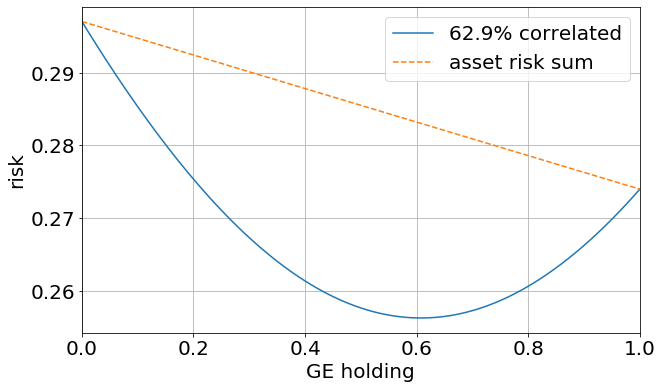
\includegraphics[width=0.7\textwidth]{figures/diversification}
\caption{Risk of a portfolio made up from IBM and General Electric against the fraction of GE stock in the portfolio. The curved line represents the risk of the portfolio; the straight line represents the sum of the two single risks.}
\label{fig:diversification}
\end{figure}

\subsection{Maximum Diversification Portfolio}
\label{maximum-diversification-portfolio}

Diversification is most often either pursued in tandem with other objective, such as return maximization, or pursued simply by including more asset classes or adding constraints based on intuition.

But it does not have to be this way and diversification can be pursued explicitly as the sole objective in portfolio construction.
In a 2008 paper~\cite{bib:diversification}, the diversification ratio $D$ of a portfolio has been defined as

\begin{equation}
D=\cfrac{\mathbf{w}^T\boldsymbol{\sigma}}{\sqrt {\mathbf{w}^T\Sigma \mathbf{w}}}
\end{equation}
where $\boldsymbol{\sigma}$ is the vector of volatilities and $\Sigma$ is the covariance matrix. The denominator represents portfolio volatility and the numerator the asset weighted average volatilities. More diversification within a portfolio decreases the denominator and leads to a higher diversification ratio.
Let's construct a portfolio that maximize this ratio.

\begin{ipythonnon}
def _sum_weights(w: np.array) -> float:
  return np.sum(w) - 1.0

def diversification_ratio(w):
  w_vol = np.dot(np.sqrt(np.diag(covariance)), w.T)
  port_vol = np.sqrt(np.dot(w.T, np.dot(covariance, w)))
  diversification_ratio = w_vol/port_vol
  return -diversification_ratio

covariance = optimizer.covariance
returns = optimizer.returns
num_assets = len(optimizer.assets)
bounds = tuple((0, 1) for asset in range(num_assets))
cons = ({'type': 'eq', 'fun': _sum_weights},)
#cons = cons + ({'type': 'ineq', 'fun': long_only_constraint},)
weights = [1./num_assets for _ in range(num_assets)]
opts = minimize(diversification_ratio, weights, bounds=bounds,
                constraints=cons)
print (opts)
\end{ipythonnon}
\begin{ioutput}
    message: Optimization terminated successfully
    success: True
     status: 0
        fun: -1.3545218215934602
          x: [ 3.500e-01  1.803e-01  1.552e-01  1.236e-01  1.909e-01]
        nit: 5
        jac: [-3.762e-04  3.166e-04 -4.323e-04  8.811e-04  1.648e-04]
       nfev: 32
       njev: 5
multipliers: [ 9.138e-05]
\end{ioutput}
\begin{ipythonnon}
ret = np.sum(returns*opts.x)
vol = np.sqrt(opts.x.T.dot(np.dot(covariance, opts.x)))
print (f"Return: {ret:.3f}")
print (f"Vol: {vol:.3f}")
print (f"Diversification: {-opts.fun:.3f}")
\end{ipythonnon}
\begin{ioutput}
Return: 0.280
Vol: 0.207
Diversification: 1.355
\end{ioutput}
Figure~\ref{fig:max_div} shows how the maximum diversified portfolio compares to the efficient frontier.

\begin{figure}[htb]
\centering
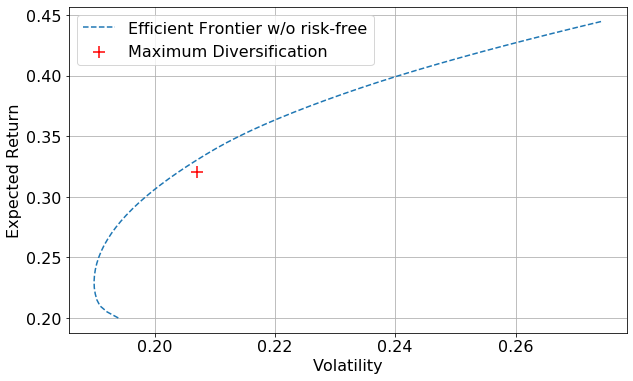
\includegraphics[width=0.7\textwidth]{figures/max_div}
\caption{Portfolio constructed with the maximum diversification technique shown in the return/variance plane.}
\label{fig:max_div}
\end{figure}

%We can see the power of diversification in another example. Given a  portfolio of $N$ stocks, each with risk $\sigma$ and uncorrelated returns, the risk of an equal-weighted portfolio of these stocks will be
%\begin{equation}
%\sigma_P = \cfrac{\sigma}{\sqrt{N}}
%\end{equation}
%
%Assume now that the correlation between the returns of all pairs of stocks is equal to $\rho$. Then the risk of an equally weighted portfolio is:
%\begin{equation}
%\sigma_P = \sigma\cdot\sqrt{\cfrac{1+\rho(N-1)}{N}};\quad \lim_{N \to +\infty} \sigma_P = \sigma\cdot\sqrt{\rho}
%\label{eq:risk_correlation}
%\end{equation}
%which can be further simplified when considering a portfolio contains a very large number of correlated stocks
%
%To get a feel for this, consider the example of an equal-weighted portfolio of the 20 Major Market Index constituent stocks. In December 1992, these stocks had an average risk of 27.8\%, while the equal-weighted portfolio has a risk of 20.4\%. Equation~\ref{eq:risk_correlation} then implies an average correlation between these stocks of 0.52.

%As we have already seen no measure of unsystematic risk appears in the risk premium, of CAPM model, since it is assumed that diversification has eliminated it.
%
%In the Markowitz model instead diversification is achieved by seeking to combine in a portfolio assets with returns that are less than perfectly positively correlated, in an effort to lower portfolio risk (variance) without sacrificing return, through the reduction of the correlation matrix $\Sigma$.

\section{Risk Parity Portfolio}
\label{risk-parity-portfolio}

An alternative approach to optimize a portfolio is given by the \emph{risk parity}. A risk parity portfolio is an investment allocation strategy which focuses on the allocation of risk, rather than on the allocation of capital.
Such a portfolio is characterized by having equal risk contributions to the total risk from each individual asset.

This allocation strategy has gained popularity in the last decades since it is believed to provide better risk adjusted return than capital based allocation strategies.

Risk parity allocation is also referred to as equally-weighted risk contributions portfolio method. Equally-weighted risk contributions is not about \emph{having the same volatility}, it is about having each asset contributing in the same way to the portfolio overall volatility. For this we will have to define the contribution of each asset to the portfolio risk.

Let's go over a very basic example to better illustrate how to construct a simple risk parity portfolio. Consider a portfolio of \(N\) assets: \(x_{1}, \ldots, x_N\) where as usual the weight of the $i^{th}$ asset is denoted by \(w_{i}\) and all the \(w_{i}\) form the allocation vector \(\mathbf{w}\). Let us further denote the covariance matrix of the assets as \(\Sigma\). The volatility of the portfolio is then defined as:

\begin{equation}
\sigma_p={\sqrt {\mathbf{w}^T\Sigma \mathbf{w}}} = \sum_{i=1}^{N}\sigma _{i}\qquad\textrm{with}~\sigma _{i} = w_{i}\cdot \cfrac{\partial\sigma_p}{\partial w_{i}}={\cfrac {w_{i}(\Sigma \mathbf{w})_{i}}{\sqrt {\mathbf{w}^T\Sigma \mathbf{w}}}}
\end{equation}
so that \(\sigma _{i}\) can be interpreted as the contribution of the $i^{th}$ asset to the overall risk of the portfolio.

\begin{attention}
\subsubsection{Derivation of $\sigma_i$}
Expressing explicitly in matrix form the standard deviation of the portfolio we get
\[
\begin{split}
\sigma_p={\sqrt {\mathbf{w}^T\Sigma \mathbf{w}}} & =
\sqrt{
	\begin{bmatrix}
	w_{1} \\
	w_{2}
	\end{bmatrix}
	\begin{bmatrix}
	\sigma_{11} & \sigma_{21} \\
	\sigma_{12} & \sigma_{22}
	\end{bmatrix}
	\begin{bmatrix}
	w_{1} & w_{2} \\
	\end{bmatrix}
}\\
&=
\sqrt{
	\begin{bmatrix}
	w_{1} \\
	w_{2}
	\end{bmatrix}
	\begin{bmatrix}
w_{1}\sigma_{11} + w_{2}\sigma_{12} & w_{1}\sigma_{21} + w_{2}\sigma_{22} \\
	\end{bmatrix}
} \\
&= \sqrt{
w_{1}w_{1}\sigma_{11} + w_{2}w_{1}\sigma_{12} + w_{1}w_{2}\sigma_{21} + w_{2}w_{2}\sigma_{22} }
\end{split}
\]
Now performing the derivative with respect to $w_1$ we obtain
\[\cfrac{\partial\sigma_p}{\partial w_1} = \cfrac{1}{2}\cdot\cfrac{2\cdot w_1\sigma_{11} + 2\cdot w_{2}\sigma_{21}}{\sigma_p} = \cfrac{w_1\sigma_{11} + w_{2}\sigma_{21}}{\sigma_p} = \cfrac{(\Sigma \mathbf{w})_{1}}{\sigma_p}\]

Summing up $\sum_{i=1}^{N} w_i\cdot\cfrac{\partial\sigma_p}{\partial w_i}$ we get back $\sigma_p$
\end{attention}

Equal risk contribution then means \(\sigma _{i} =\sigma _{j}\) for all \(i,j\) or equivalently \(\sigma _{i}=\sigma_p/N\). So

\begin{equation}
\sigma _{i} = \cfrac{\sigma_p}{N}={\cfrac {w_{i}(\Sigma \mathbf{w})_{i}}{\sqrt {\mathbf{w}^T\Sigma \mathbf{w}}}}\implies w_{i} = \frac {\sigma_p^{2}}{(\Sigma \mathbf{w})_{i}N}
\label{eq:risk_parity_weights}
\end{equation}
Since we want the previous expression to be true for each $i$, the solution for the weights can be found by solving the minimization problem

\begin{equation}
\underset{\mathbf{w}}{\min } \sum _{i=1}^{N}\left[w_{i}-{\frac {\sigma_p^{2}}{(\Sigma \mathbf{w})_{i}N}}\right]^{2}
\end{equation}
\noindent
where ideally it is required to be 0 the difference between the squared sum of the weights and the theoretical values expressed by Eq~\ref{eq:risk_parity_weights}.

Going back to our data sample let's find out the weights to give us a risk parity portfolio.

\pythoncodenon{code/portfolios_risk_parity.py}
Figure~\ref{fig:risk_parity} shows the fraction of risk allocated to each asset with the corresponding weight within the portfolio.

\begin{figure}[htb]
\centering
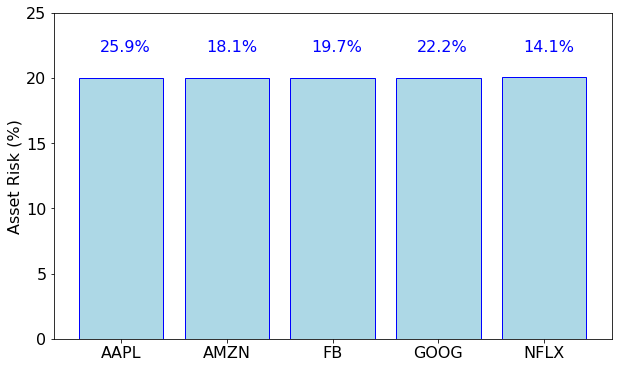
\includegraphics[width=0.7\textwidth]{figures/risk_parity}
\caption{Fraction of risk allocated among the assets of a portfolio. The blue numbers show the corresponding weight of each asset.}
\label{fig:risk_parity}
\end{figure}

\subsection{Risk Budget Allocation}
\label{risk-budget-allocation}

The same technique can be used if we would like to calculate a portfolio with risk budget allocation. In this case we want to associate to each asset a particular level of risk.We can now change the previous equation which was setting every asset risk contribution fraction to $1/N$

\begin{equation}
\sigma _{i}=\cfrac{\sigma_p}{N}
\end{equation}
and replace it with the desired fraction of risk (\(f_i\)) specific for each asset

\begin{equation}
\sigma _{i}=f_i \cdot \sigma_p
\end{equation}
so that the relation to minimize becomes

\begin{equation}
\underset{\mathbf{w}}{\min} \sum _{i=1}^{N}\left[w_{i}-{\frac {f_i \cdot \sigma_p^{2}}{(\Sigma \mathbf{w})_{i}}}\right]^{2}
\end{equation}
\noindent
Translating it into \texttt{python} we get:

\pythoncodenon{code/portfolios_budget_allocation.py}
Figure~\ref{fig:risk_allocation} shows the amount of risk associated to each asset and its weight within the portfolio.
Indeed for each stock we have allocated the desired amount of risk.

\begin{figure}[htb]
\centering
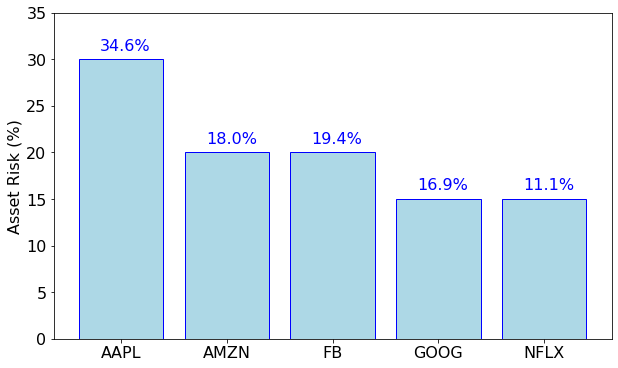
\includegraphics[width=0.7\textwidth]{figures/risk_allocation}
\caption{Fraction of risk allocated among the assets of a portfolio. The blue numbers show the corresponding weight of each asset.}
\label{fig:risk_allocation}
\end{figure}

\section{Black-Litterman Allocation}
\label{sec:black-litterman}
The Black-Litterman (BL) model, established for the first time in the early 1990’s by Fischer Black and Robert Litterman, is a sophisticated strategy for dealing with portfolios. It takes a Bayesian approach~\ref{cap:bayes} to asset allocation. Specifically, it combines a \emph{prior estimate} of returns (for example, the market-implied returns) with views on certain assets, to produce a \emph{posterior estimate} of expected returns. The advantages of this approach are:
\begin{itemize}
	\item you can provide views on only a subset of assets and BL will meaningfully propagate it, taking into account the covariance with other assets;
	\item you can provide confidence in your views;
	\item using Black-Litterman posterior returns results in much more stable portfolios than using mean-historical return (the most important input in mean-variance optimization is the vector of expected returns; however it has been shown that a small increase in the expected return of one of the portfolio's assets can force half of the assets from the portfolio).
\end{itemize}

Essentially, Black-Litterman treats the vector of expected returns itself as a quantity to be estimated. The Black-Litterman formula is given below
\begin{equation}
	\mathbb{E}[R] = [(\tau\Sigma)^{-1}+P^T\Omega^{-1}P]^{-1}[(\tau\Sigma)^{-1}\Pi + P^T\Omega^{-1}Q]
	\label{eq:bl_formula}
\end{equation}
where $\mathbb{E}[R]$ is a $N\times1$ vector of expected returns, where $N$ is the number of assets, $Q$ is a $K\times1$ vector of views, $P$ is the $K\times N$ picking matrix which maps views to the universe of assets (it tells the model which view corresponds to which asset(s)), $\Omega$ is the $K\times K$ uncertainty matrix of views, $\Pi$ is the $N\times 1$ vector of prior expected returns, $\Sigma$ is the $N\times N$ covariance matrix of asset returns, and $\tau$ is a scalar tuning constant.

Though the formula appears to be quite unwieldy, it turns out that simply represents a \emph{weighted average} between the prior estimate of returns and the views, where the weighting is determined by the confidence in the views and the parameter $\tau$.

Similarly, a posterior estimate of the covariance matrix can be calculated
\begin{equation}
	\hat{\Sigma} = \Sigma +[(\tau \Sigma)^{-1} + P^T \Omega^{-1}P]^{-1}
\end{equation}

\begin{attention}
	In real-world scenarios matrix inversion can be tricky or lead to nonsensical results. So a safer expression for the Black-Litterman model not involving matrix inversion can be derived using the following result
	\begin{equation*}
		(A+BDB^T)^{-1} = A^{-1} - A^{-1}B(B^TA^{-1}B+D^{-1})^{-1}BTA^{-1}
	\end{equation*}
	Starting from Eq.~\ref{eq:bl_formula} and applying previous result to the first member of right-hand side with $A=\Sigma^{-1}, B=P^T, D=\Omega^{-1}$,
	we get (for simplicity we set $\tau=1$)
	\begin{equation}
		\begin{aligned}
			\mathbb{E}[R] &= [\Sigma^{-1}+P^T\Omega^{-1}P]^{-1}[\Sigma^{-1}\Pi + P^T\Omega^{-1}Q] \\
			&= [\Sigma - \Sigma P^T(P\Sigma P^T + \Omega)^{-1} P\Sigma][\Sigma^{-1}\Pi + P^T\Omega^{-1}Q] \\
			&= \Pi + \Sigma P^T\Omega^{-1}Q - \Sigma P^T(\ldots)P\Pi - \Sigma P^T(\ldots)^{-1} P\Sigma P^T\Omega^{-1}Q] \\
			&= \Pi + \Sigma P^T(\ldots)^{-1} P\Pi + \Sigma P^T[I - (\ldots)^{-1}P\Sigma P^T]\Omega^{-1}Q \\
			&= \Pi + \Sigma P^T(\ldots)^{-1} P\Pi + \Sigma P^T[(\ldots)^{-1} (\ldots) - (\ldots)^{-1}P\Sigma P^T]\Omega^{-1}Q \\
			&= \Pi + \Sigma P^T(\ldots)^{-1} P\Pi + \Sigma P^T(\ldots)^{-1} \Omega\Omega^{-1}Q \\
			&= \Pi + \Sigma P^T{\underbrace{(P\Sigma P^T + \Omega)}_{A}}^{-1} \underbrace{(Q- P\Pi)}_{b} = \Pi + \Sigma P^T x \\
		\end{aligned}
	\end{equation}
	In the last expression $x$ can be found by solving $Ax=b$ hence completely avoiding inversions.
\end{attention}

\subsection{Priors}
The Black-Litterman model uses “equilibrium” returns as a neutral starting point (i.e. priors). Equilibrium returns are the set of returns that clear the market.
You can think of the prior as the "default" estimate, in the absence of any information. Black and Litterman~\cite{bib:black_litterman} provide the insight that a natural choice for this prior is the market’s estimate of the return, which is embedded into the market capitalization of the asset.

Every asset in the market portfolio contributes a certain amount of risk to the portfolio. Standard theory suggests that investors must be compensated for the risk that they take, so we can attribute to each asset an expected compensation (i.e prior estimate of returns). This is quantified by the market-implied risk premium, which is the market’s excess return divided by its variance:
\begin{equation}
	\delta = \frac{R-R_f}{\sigma^2}
\end{equation}

The risk-aversion coefficient ($\delta$) characterizes the expected risk-return trade-off. It is the rate at which an investor will forego expected return for less variance. In the reverse optimization process, the risk aversion coefficient acts as a scaling factor for the reverse optimization estimate of excess returns; the weighted reverse optimized excess returns equal the specified market risk premium. More excess return per unit of risk (a larger delta) increases the estimated excess returns.

The equilibrium returns (or market-implied returns) are derived using a \emph{reverse optimization} method in which the vector of implied excess equilibrium returns is extracted
\begin{equation}
	\Pi=\delta \Sigma w_{mkt}
\end{equation}

Here, $w_{mkt}$ denotes the market-cap weights. This formula is calculating the total amount of risk contributed by an asset and multiplying it with the market price of risk, resulting in the market-implied returns vector$\Pi$.

Clearly, there is nothing stopping you from using any prior you see fit (but it must have the same dimensionality as the universe). If you think that the mean historical returns are a good prior, you could go with that. But a significant body of research shows that mean historical returns are a completely uninformative prior.

\subsection{Views}
More often than not, investment managers have specific views regarding the expected return of some of the assets in a portfolio, which differ from the Implied Equilibrium return.
In the Black-Litterman model, users can either provide absolute or relative views. Absolute views are statements like: “AAPL will return 10\%” or “XOM will drop 40\%”. Relative views, on the other hand, are statements like “GOOG will outperform FB by 3\%”.
Note that the model does not require that investors specify views on all assets.

These views must be specified in the vector $Q$ and mapped to the asset universe via the picking matrix $P$. A brief example of this is shown below, though a comprehensive guide is given by~\cite{bib:Idzorek}.
Let’s say that our universe is defined by the \emph{ordered} list: SBUX, GOOG, FB, AAPL, BAC, JPM, T, GE, MSFT, XOM. We want to represent four views on these 10 assets, two absolute and two relative:
\begin{itemize}
	\item SBUX will drop 20\% (absolute);
	\item MSFT will rise by 5\% (absolute);
	\item GOOG outperforms FB by 10\%;
	\item BAC and JPM will outperform T and GE by 15\%.
\end{itemize}

The corresponding views vector is formed by taking the numbers above and putting them into a column:
\begin{equation}
	Q = \begin{bmatrix}-0.20 \\ 0.05\\ 0.10\\ 0.15\\\end{bmatrix}
\end{equation}

The picking matrix is more interesting. Remember that its role is to link the views (which mention 8 assets) to the universe of 10 assets. Arguably, this is the most important part of the model because it is what allows us to propagate our expectations (and confidences in expectations) into the model:
\begin{equation}
	P = \begin{bmatrix}
		1 & 0 & 0 & 0 & 0 & 0 & 0 & 0 & 0 & 0 \\
		0 & 0 & 0 & 0 & 0 & 0 & 0 & 0 & 1 & 0 \\
		0 & 1 & -1 & 0 & 0 & 0 & 0 & 0 & 0 & 0 \\
		0 & 0 & 0 & 0 & 0.5 & 0.5 & -0.5 & -0.5 & 0 & 0 \\
	\end{bmatrix}
\end{equation}

Each view has a corresponding row in the picking matrix (the order matters): in particular absolute views have a single 1 in the column corresponding to the ticker’s order in the universe, relative views have a positive number in the nominally outperforming asset columns and a negative number in the nominally under-performing asset columns. The numbers in each row should sum up to 0.

\subsection{Confidence matrix and $\tau$}

Except in the hypothetical case in which a clairvoyant investor is 100\% confident in the expressed view, it is required to set a level of confidence on the views. Determining the individual variances of the error terms ($\omega$) that constitute the diagonal elements of $\Omega$ is one of the most complicated aspects of the model.

The confidence matrix is a diagonal covariance matrix containing the variances of each view. One heuristic for calculating $\Omega$ is to say that is proportional to the variance of the priors. This is a reasonable assumption since quantities that move around a lot are harder to forecast. The off-diagonal elements of $\Omega$ are 0’s because the model assumes that the views are independent of one another. Hence
\begin{equation}
	\Omega = \tau \cdot P\Sigma P^T
\end{equation}

An alternative way for defining $\Omega$ is provided in~\cite{bib:Idzorek}, this allows you to specify your view uncertainties as percentage confidences, but it is not described here.

Another parameter that controls the relative weighting of the priors views is $\tau$. There is a lot to be said about tuning this parameter, with many contradictory rules of thumb. Indeed, there has been an entire paper written on it~\cite{bib:tau}.
%We choose the sensible default τ=0.05.

The scalar $\tau$ is more or less inversely proportional to the relative weight given to the Implied Equilibrium Return Vector ($\Pi$). Unfortunately, guidance in the literature for setting the scalar’s value is scarce. Since the uncertainty in the mean is less than the uncertainty in the return, $\tau$ should be close to zero (one would expect the Equilibrium Returns to be less volatile than the historical returns).

%Somebody sets its value between 0.01 and 0.05, and then calibrates the model based on a target level of tracking error.
%Conversely, Satchell and Scowcroft (2000) say the value of the scalar ($\tau$) is often set to 1.10 Finally, Blamont and Firoozye (2003) interpret $\tau\Sigma$ as the standard error of estimate of the Implied Equilibrium Return Vector ($Pi$); thus, the scalar is approximately 1 divided by the number of observations.

Nevertheless turns out that for the two specific definition of $\Omega$ outlined above the value of $\tau$ does not matter. This is a consequence of the mathematics: the $\tau$ cancels in the matrix multiplications.
When the covariance matrix of the error term $\Omega$ is calculated using the methods outlined above, the actual value of the scalar $\tau$ becomes irrelevant because only the ratio $\omega/\tau$ enters the model. For example, changing the assumed value of $\tau$ from 0.025 to 15 dramatically changes the value of the diagonal elements of $\Omega$, but the new $\mathbb{E}[R]$ is unaffected.

\subsection{Output of the BL model}
Conceptually, the Black-Litterman model is a complex, weighted average of the Implied Equilibrium Return Vector ($\Pi$) and the View Vector ($Q$), in which the relative weightings are a function of the scalar ($\tau$) and the uncertainty of the views ($\Omega$).
Unfortunately, the scalar and the uncertainty in the views are the most abstract and difficult to specify parameters of the model. The greater the level of confidence (certainty) in the expressed views, the closer the new return vector will be to the views.
If the investor is less confident in the expressed views, the new return vector should be closer to the Implied Equilibrium Return Vector ($\Pi$).

The BL model outputs posterior estimates of the returns and covariance matrix. The default suggestion in literature is to then input these into an optimizer, i.e. find the weights that minimize the risk (or maximize the return) given the posteriors. A quick alternative, which may be useful especially for fast checks, is to calculate the weights implied by the returns vector~\cite{bib:walters}.
It is actually the reverse of the procedure we used to calculate the returns implied by the market weights
\begin{equation}
	w = (\delta\Sigma)^{-1}\mathbb{E}[R]
\end{equation}

In the absence of constraints, the Black-Litterman model only recommends a departure from an asset’s market capitalization weight if it is the subject of a view. The magnitude of their departure from their market capitalization weight is controlled by the ratio of the scalar ($\tau$) to the variance of the error term ($\omega$) of the view in question. $\omega$ is inversely related to the investor’s confidence in that particular view (e.g. 0 represents 100\% confidence, complete certainty, in the view). The magnitude of the departure from the market capitalization weights is also affected by other views. %Additional views lead to a different Combined Return Vector ( E[R]), which leads to a new vector of recommended weights.

Having specified $\tau$ and the covariance matrix of the error term $\Omega$, all inputs are entered into the Black-Litterman formula and the New Combined Return Vector ($\mathbb{E}[R]$) is derived.

\newpage
\section*{Exercises}
\begin{question}
One of the approaches to finding the optimal point on the efficient frontier for a given investor is to maximize the investor's utility ($U$). This is a measure of how much benefit investors obtain from portfolio performance. Utility is a measure of relative satisfaction that an investor derives from different portfolios. Utility is a function of the portfolio expected return, the portfolio variance and a measure of risk aversion

\begin{equation*}
U = \mathbb{E}(R_{p}) - \frac{1}{2}A\sigma^2
\end{equation*}
where $U$ = utility, $\mathbb{E}(R)$ = portfolio expected return, $A$ = risk aversion coefficient and $\sigma^2$ = portfolio variance.
In determining the risk aversion ($A$), we measure the marginal reward an investor needs in order to take on more risk. A risk-averse investor will need a high margin reward for taking on more risk. The utility equation shows the following:
\begin{itemize}
\tightlist
\item $U$ can be positive or negative, i.e. it is unbounded;
\item high returns add to utility;
\item high variance reduces utility;
\item $U$ does not measure satisfaction but can be used to rank portfolios.
\end{itemize}

The risk aversion coefficient, $A$, ranges between 1 and 10 (1 for the aggressive investor, 4 for the moderate investor, and 10 for the risk-averse investor.

Given the historical series in \href{https://github.com/matteosan1/finance_course/raw/master/input_files/share_price.csv}{share\_prices.csv} find the best portfolio for aggressive, moderate and risk-averse investors.

\end{question}

\cprotEnv \begin{solution}
\begin{ipython}
import pandas as pd
df = pd.read_csv("share_prices.csv", index_col='Date')
daily_returns = df.pct_change()
returns = daily_returns.mean()*252
covariance = daily_returns.cov()*252

print (returns)
print (covariance)
\end{ipython}
\begin{ioutput}
CHD     0.062666
COST    0.247429
CTRE    0.165151
ENTR    0.002445
HI      0.223906
LDOS    0.075464
TDS    -0.003953
TMUS    0.283815
UEC     0.999521
WM      0.163298
dtype: float64

           CHD     COST       CTRE      ENTR        HI      LDOS       TDS
CHD   0.067815  0.036114  0.016454  0.022583  0.022301  0.029738  0.032921   
COST  0.036114  0.073004  0.031599  0.049279  0.034606  0.034481  0.034043   
CTRE  0.016454  0.031599  0.313706  0.074262  0.136719  0.068927  0.088424   
ENTR  0.022583  0.049279  0.074262  0.113892  0.062266  0.043155  0.040843   
HI    0.022301  0.034606  0.136719  0.062266  0.202751  0.068284  0.097420   
LDOS  0.029738  0.034481  0.068927  0.043155  0.068284  0.110635  0.059296   
TDS   0.032921  0.034043  0.088424  0.040843  0.097420  0.059296  0.185842   
TMUS  0.026069  0.042121  0.073199  0.055806  0.057519  0.046704  0.068516   
UEC   0.045100  0.099269  0.164647  0.147985  0.165341  0.096700  0.143037   
WM    0.034987  0.034676  0.049294  0.034555  0.057760  0.047310  0.048338   
...
\end{ioutput}
\begin{ipython}
import numpy as np
from scipy.optimize import minimize

def sum_weights(w): 
    return np.sum(w) - 1

def utility(w, returns, cov, risk_aversion):
    return -(returns.dot(w) - 0.5*w.T.dot(cov.dot(w))*risk_aversion)

num_assets = 10
constraints = [{'type': 'eq', 'fun': sum_weights},] 
bounds = tuple((0, 1) for _ in range(num_assets))
weights = [1./num_assets for _ in range(num_assets)]

for risk_aversion in (1, 4, 10):
  opts = minimize(utility, weights, args=(returns, covariance, risk_aversion),
                bounds=bounds, constraints=constraints)
  for i, c in enumerate(df.columns):
    print ("{} {:.1f}".format(c, opts.x[i]*100), end=" ")
  print()
  print ("Expected return: {:.3f}".format(opts.x.dot(returns)))
  print ("Variance: {:.3f}".format(opts.x.T.dot(covariance.dot(opts.x))))
\end{ipython}
\begin{ioutput}
# aggressive
CHD 0.0 COST 0.0 CTRE 0.0 ENTR 0.0 HI 0.0 LDOS 0.0 TDS 0.0 TMUS 12.8 UEC 87.2 WM 0.0 
Expected return: 0.908
Variance: 0.734

# moderate
CHD 0.0 COST 47.2 CTRE 0.0 ENTR 0.0 HI 0.0 LDOS 0.0 TDS 0.0 TMUS 33.1 UEC 18.3 WM 1.4 
Expected return: 0.396
Variance: 0.104

# risk averse
CHD 7.1 COST 40.2 CTRE 0.0 ENTR 0.0 HI 1.3 LDOS 0.0 TDS 0.0 TMUS 22.7 UEC 4.1 WM 24.6 
Expected return: 0.252
Variance: 0.055
\end{ioutput}
\end{solution}

\begin{question}
Your are portfolio manager and one of your clients is asking to design her investment in order to reduce at the minimum the risk. Her position involves these shares: 'TMUS', 'TDS', 'ENTR', 'UEC', 'WM', 'CTRE', 'LDOS', 'COST', 'CHD', 'HI'.
Find the weights corresponding to each asset.

\noindent\textbf{Hint:} the historical series of the corresponding companies are stored in \href{https://github.com/matteosan1/finance_course/raw/master/input_files/share_price.csv}{share\_prices.csv}.

\end{question}

\cprotEnv \begin{solution}
\begin{ipython}
import pandas as pd
df = pd.read_csv("share_prices.csv", index_col='Date')

daily_returns = df.pct_change()
returns = daily_returns.mean()*252
covariance = daily_returns.cov()*252
\end{ipython}
\begin{ipython}
import numpy as np
from scipy.optimize import minimize

def sum_weights(w):
    return np.sum(w) - 1

def min_risk(w, cov):
    return np.sqrt(w.T.dot(cov.dot(w)))

num_assets = 10
constraints = ({'type': 'eq', 'fun': sum_weights},)
bounds = tuple((0, 1) for asset in range(num_assets))
weights = [1./num_assets for _ in range(num_assets)]
opts = minimize(min_risk, weights, args=(covariance,),
                bounds=bounds, constraints=constraints)

print (opts)
\end{ipython}
\begin{ioutput}
     fun: 0.20887087318996655
     jac: array([0.2088003 , 0.20897953, 0.20895358, 0.20911743, 0.21106115,
                 0.20858843, 0.20914311, 0.20901022, 0.40519709, 0.20881298])
 message: 'Optimization terminated successfully'
    nfev: 110
     nit: 10
    njev: 10
  status: 0
 success: True
       x: array([3.33744344e-01, 1.68530140e-01, 8.18977235e-03, 9.91808728e-02,
                 0.00000000e+00, 7.10377889e-02, 6.05724516e-03, 8.44657341e-02,
                 3.89635156e-20, 2.28794102e-01])
\end{ioutput}
\begin{ipython}
print ("Portfolio composition")
for i, n in enumerate(df.columns):
    print ("{:5}: {:4.1f}%".format(n, opts.x[i]*100))
print ("Portfolio variance: {:.4f}".format(opts.fun**2))
print ("Expected Portfolio return: {:.3f}".format(opts.x.dot(returns)))
\end{ipython}
\begin{ioutput}
Portfolio composition
CHD  : 33.4%
COST : 16.9%
CTRE :  0.8%
ENTR :  9.9%
HI   :  0.0%
LDOS :  7.1%
TDS  :  0.6%
TMUS :  8.4%
UEC  :  0.0%
WM   : 22.9%
Portfolio variance: 0.0436
Expected Portfolio return: 0.131
\end{ioutput}
\end{solution}

%\begin{question}[title={(Return Allocation Portfolio)}]
%After few months the same client of the previous question, contacted you again asking for larger returns. In particular she would like to increase it by 40\%.
%Find the new portfolio composition that makes your client happy.
%\end{question}
%\begin{solution}
%\begin{tcolorbox}[size=fbox, boxrule=1pt, colback=cellbackground, colframe=cellborder]
%\begin{Verbatim}[commandchars=\\\{\}]
%\PY{k}{def} \PY{n+nf}{efficient\PYZus{}frontier}\PY{p}{(}\PY{n}{w}\PY{p}{,} \PY{n}{asset\PYZus{}returns}\PY{p}{,} \PY{n}{target\PYZus{}return}\PY{p}{)}\PY{p}{:} 
%    \PY{n}{portfolio\PYZus{}return} \PY{o}{=} \PY{n}{np}\PY{o}{.}\PY{n}{sum}\PY{p}{(}\PY{n}{asset\PYZus{}returns} \PY{o}{*} \PY{n}{w}\PY{p}{)} 
%    \PY{k}{return} \PY{p}{(}\PY{n}{portfolio\PYZus{}return} \PY{o}{\PYZhy{}} \PY{n}{target\PYZus{}return}\PY{p}{)}
%		
%\PY{n}{results} \PY{o}{=} \PY{p}{[}\PY{p}{]}
%\PY{n}{bounds} \PY{o}{=} \PY{n+nb}{tuple}\PY{p}{(}\PY{p}{(}\PY{l+m+mi}{0}\PY{p}{,} \PY{l+m+mi}{1}\PY{p}{)} \PY{k}{for} \PY{n}{asset} \PY{o+ow}{in} \PY{n+nb}{range}\PY{p}{(}\PY{n}{num\PYZus{}assets}\PY{p}{)}\PY{p}{)}
%\PY{n}{target} \PY{o}{=} \PY{l+m+mf}{0.172}\PY{o}{*}\PY{l+m+mf}{1.4}
%\PY{n}{constraints} \PY{o}{=} \PY{p}{(}\PY{p}{\PYZob{}}\PY{l+s+s1}{\PYZsq{}}\PY{l+s+s1}{type}\PY{l+s+s1}{\PYZsq{}}\PY{p}{:} \PY{l+s+s1}{\PYZsq{}}\PY{l+s+s1}{eq}\PY{l+s+s1}{\PYZsq{}}\PY{p}{,} \PY{l+s+s1}{\PYZsq{}}\PY{l+s+s1}{fun}\PY{l+s+s1}{\PYZsq{}}\PY{p}{:} \PY{n}{efficient\PYZus{}frontier}\PY{p}{,} 
%                \PY{l+s+s1}{\PYZsq{}}\PY{l+s+s1}{args}\PY{l+s+s1}{\PYZsq{}}\PY{p}{:}\PY{p}{(}\PY{n}{returns}\PY{p}{,} \PY{n}{target}\PY{p}{)}\PY{p}{\PYZcb{}}\PY{p}{,}
%               \PY{p}{\PYZob{}}\PY{l+s+s1}{\PYZsq{}}\PY{l+s+s1}{type}\PY{l+s+s1}{\PYZsq{}}\PY{p}{:} \PY{l+s+s1}{\PYZsq{}}\PY{l+s+s1}{eq}\PY{l+s+s1}{\PYZsq{}}\PY{p}{,} \PY{l+s+s1}{\PYZsq{}}\PY{l+s+s1}{fun}\PY{l+s+s1}{\PYZsq{}}\PY{p}{:} \PY{n}{sum\PYZus{}weights}\PY{p}{\PYZcb{}}\PY{p}{)}
%\PY{n}{weights} \PY{o}{=} \PY{p}{[}\PY{l+m+mf}{1.}\PY{o}{/}\PY{n}{num\PYZus{}assets} \PY{k}{for} \PY{n}{\PYZus{}} \PY{o+ow}{in} \PY{n+nb}{range}\PY{p}{(}\PY{n}{num\PYZus{}assets}\PY{p}{)}\PY{p}{]}
%\PY{n}{opts} \PY{o}{=} \PY{n}{minimize}\PY{p}{(}\PY{n}{markowitz}\PY{p}{,} \PY{n}{weights}\PY{p}{,} \PY{n}{args}\PY{o}{=}\PY{p}{(}\PY{n}{covariance}\PY{p}{,}\PY{p}{)}\PY{p}{,}
%\PY{n}{bounds}\PY{o}{=}\PY{n}{bounds}\PY{p}{,} \PY{n}{constraints}\PY{o}{=}\PY{n}{constraints}\PY{p}{)} 
%		
%\PY{n}{p\PYZus{}variance} \PY{o}{=} \PY{n}{np}\PY{o}{.}\PY{n}{dot}\PY{p}{(}\PY{n}{opts}\PY{o}{.}\PY{n}{x}\PY{o}{.}\PY{n}{T}\PY{p}{,} \PY{n}{np}\PY{o}{.}\PY{n}{dot}\PY{p}{(}\PY{n}{covariance}\PY{p}{,} \PY{n}{opts}\PY{o}{.}\PY{n}{x}\PY{p}{)}\PY{p}{)}
%\PY{n}{ret} \PY{o}{=} \PY{n}{np}\PY{o}{.}\PY{n}{sum}\PY{p}{(}\PY{n}{returns}\PY{o}{*}\PY{n}{opts}\PY{o}{.}\PY{n}{x}\PY{p}{)}
%\PY{n+nb}{print} \PY{p}{(}\PY{l+s+s2}{\PYZdq{}}\PY{l+s+s2}{Portfolio variance: }\PY{l+s+si}{\PYZob{}:.3f\PYZcb{}}\PY{l+s+s2}{\PYZdq{}}\PY{o}{.}\PY{n}{format}\PY{p}{(}\PY{n}{variance}\PY{p}{)}\PY{p}{)}
%\PY{n+nb}{print} \PY{p}{(}\PY{l+s+s2}{\PYZdq{}}\PY{l+s+s2}{Portfolio return: }\PY{l+s+si}{\PYZob{}:.3f\PYZcb{}}\PY{l+s+s2}{\PYZdq{}}\PY{o}{.}\PY{n}{format}\PY{p}{(}\PY{n}{ret}\PY{p}{)}\PY{p}{)}
%
%Portfolio variance: 0.026
%Portfolio return: 0.241
%\end{Verbatim}
%\end{tcolorbox}	
%\end{solution}

\begin{question}
The client is not yet satisfied and decides to move to a risk parity portfolio. Compute the correct weights to have each asset contributing equally to the portfolio risk.
\end{question}

\cprotEnv \begin{solution}
\begin{ipython}
def risk_parity(w, cov):
    variance = w.T.dot(cov.dot(w))
    sum = 0 
    N = len(w)
    for i in range(N):
        sum += (w[i] - (variance/(N*(cov.dot(w))[i])))**2
    return sum

args = (covariance,)
constraints = ({'type': 'eq', 'fun': sum_weights})
bounds = tuple((0, 1) for asset in range(num_assets))
weights = [1./num_assets for _ in range(num_assets)]
opts = minimize(risk_parity, weights, args=(covariance,),
                bounds=bounds, constraints=constraints)

print (opts)
\end{ipython}
\begin{ioutput}
     fun: 3.5766519241779855e-07
     jac: array([ 1.24834913e-03,  1.00388202e-03, -2.28052647e-04,  6.19051279e-04,
                 -5.68149005e-04, -1.03169022e-03, -1.24285291e-03, -4.09550915e-04,
                 -2.02491654e-03,  6.26250036e-06])
 message: 'Optimization terminated successfully'
    nfev: 80
     nit: 7
    njev: 7
  status: 0
 success: True
       x: array([0.161952  , 0.12997992, 0.07022277, 0.10331577, 0.07717795,
                 0.10490077, 0.08475445, 0.10276264, 0.04079525, 0.12413849])
\end{ioutput}
\begin{ipython}
sigma_i = []
for i in range(num_assets):
    std = np.sqrt(opts.x.T.dot(covariance.dot(opts.x)))
    a = opts.x[i]*covariance.dot(opts.x)[i]
    sigma_i.append(a/std)

for i in range(num_assets):
    print ("Risk contribution for asset {}: {:6.3f}%"
           .format(i, sigma_i[i]/sum(sigma_i)*100))
\end{ipython}
\begin{ioutput}
Risk contribution for asset 0:  9.986%
Risk contribution for asset 1: 10.003%
Risk contribution for asset 2:  9.971%
Risk contribution for asset 3:  9.987%
Risk contribution for asset 4: 10.014%
Risk contribution for asset 5:  9.998%
Risk contribution for asset 6: 10.047%
Risk contribution for asset 7:  9.976%
Risk contribution for asset 8: 10.023%
Risk contribution for asset 9:  9.995%		
\end{ioutput}
\end{solution}



r\chapter{Linear Models}
\label{linear-models}

\section{Simple Linear Regression Analysis}
\label{sec:linear-regression}
Regression Analysis is a form of predictive analysis.
In particular the single (or simple) \emph{linear regression} model expresses the (linear) relationship between the dependent variable and one independent variable. The regression analysis attempts to find the strength of that relationship. For example this can be used to find the relation of a company’s performance to the industry performance or competitor business.

Regression models are expressed by an equation representing the dependent variable as a function of the independent variable. A simple linear model can be described by the following equation:
\begin{equation}
y = \beta x + \alpha + \epsilon
\label{eq:linear_regression}
\end{equation}
where $y$ is the dependent variable (target), $\alpha$ the intercept, $\beta$ the slope, $x$ the independent variable (predictor), and $\epsilon$ the residual (error).

The purpose is to estimate the underlying relationship so that we can predict the target variable based on the other (predictor).

\subsection{Ordinary Least Squares}
We need to solve a problem when running the regression model, and this is to fit a straight line to a set of pairs of observations of the dependent and independent variables. The line of best fit is where the sum of the squares of the vertical deviations (distances) between observation points and the line is at its minimum. This is the method of ordinary least squares (OLS) and the one we most commonly apply to a linear regression model.

\begin{figure}[htbp]
	\centering
	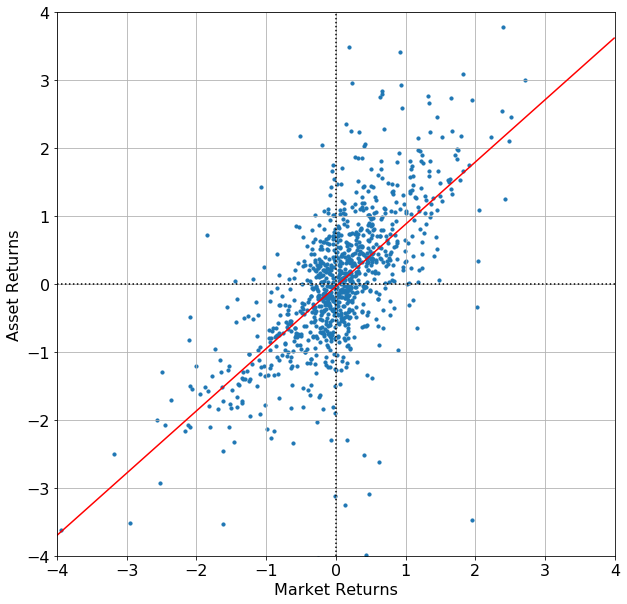
\includegraphics[width=0.7\textwidth]{figures/linear_regression}
	\caption{Example of linear regression.}
	\label{fig:linear_regression_example}
\end{figure}

The regression equation gives no exact prediction of the target value for any predictor variable. The regression coefficients we calculate from our sample data observations are only the best estimate of the real population variables.
This is why we introduce $\epsilon$ (residual/error) to the model, it covers the element of chance that an independent variable can experience variations.

\subsubsection{Covariance}
One of the measures we get from a regression analysis is the covariance

\begin{equation}
\text{Cov}(x, y) = \mathbb{E}[(x - \mathbb{E}[x])(y - \mathbb{E}[y])]
\end{equation}
where: $x$ and $y$ are the values of the independent and dependent variables at each observation.

The formula measures the direction of the relationship: if one variable is going up when the other is going down, then the covariance will be negative, and vice versa.

\subsubsection{Correlation}
That’s where correlation, another measure of regression analysis, comes in. It helps us to standardize the covariance to be able to better understand it.

Correlation takes the covariance and divides it over the product of the standard deviations of the variables. This makes sure we get a correlation coefficient between -1 and +1.
\begin{equation}
\corr(x, y) = \frac{\cov(x, y)}{\std(x)\std(y)}
\end{equation}

A correlation of +1 suggests the two variables are perfectly positively correlated, and a value of -1 suggests an entirely negative correlation.

From the definition of the $\beta$ coefficient (i.e. the slope of the linear regression) through least squares we have
\begin{equation}
\hat{\beta} = \corr(x, y)\cdot \frac{\std(y)}{\std(x)}
\end{equation}
therefore the two only coincide when $\std(y) = \std(x)$ That is, they only coincide when the two variables are, in some sense, on the same scale.

Correlation and slope at some extent give the same information, i.e. they each tell the linear relationship strength between $x$ and $y$. But, they also do each give distinct information:
\begin{itemize}
\item the correlation gives you a bounded measurement that can be interpreted independently of the two variables scale. The closer the estimated correlation is to $\pm1$, the closer the two are to a perfect linear relationship. The regression slope, in isolation, does not tell you that piece of information.
\item the regression slope gives a useful quantity interpreted as the estimated change in the expected value of $y$ for a given value of $x$. Specifically, $\hat{\beta}$ tells you the change in the expected value of $y$ corresponding to a 1-unit increase in $x$. This information can not be deduced from the correlation coefficient alone.
\end{itemize}

\subsection{Multiple Linear Regression}
Simple regression is usually not enough in a real-life scenario, as targets (dependent variables) are rarely impacted only by a single predictor. The natural extention is given by the \emph{multiple linear regression} model which can have two or more independent variables.

The function to represent the regression equation now becomes:
\begin{equation}
y = \beta_1 x_1 + \beta_2 x_2 + \ldots + \beta_n x_n + \alpha + \epsilon
\label{eq:multiple_regression}
\end{equation}

It is crucial to keep in mind that the multiple regression model requires \emph{non-collinearity}. This means the independent variables should have a minimal correlation between them. Otherwise, it is difficult to assess the real relationship between the dependent (target) and the independent (predictors) variables.

%\subsection{Linear Regression Example}
%
%The Chinese Yuan (CNY) was pegged to the US Dollar (USD) prior to July 2005. Then, China announced that the exchange rate would be set with reference to a basket of other currencies, allowing for a movement of up to 0.3\% within any given day. The actual currencies and their basket weights are unannounced by China. Figure~\ref{fig:yuan_rate} reports the Yuan exchange rate to USD between 1999 and 2013.
%
%\begin{figure}[htbp]
%\centering
%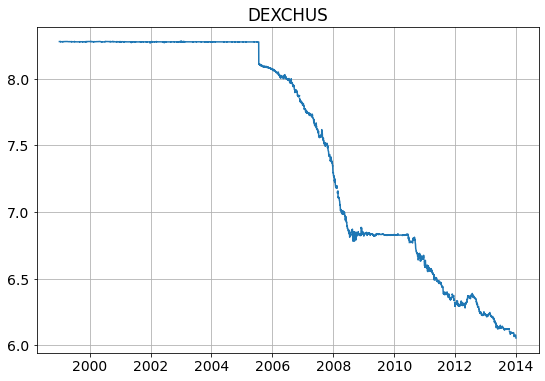
\includegraphics[width=0.7\textwidth]{figures/yuan_exchange_rate}
%\caption{Yuan exchange rate to USD from January 1999 to December 2013.}
%\label{fig:yuan_rate}
%\end{figure}
%
%From an empirical point of view, there are several important questions:
%\begin{itemize}
%\item for any given period, what is the implicit reference basket for the Chinese currency ?
%\item has the reference basket changed over time ?
%\item has the Chinese currency depreciated with respect to the dollar? If so, how much and when?
%\end{itemize}
%
%A possible approach for evaluating the implicit exchange rate regime of the Yuan involves the regression of the changes in the target currency on changes in the values of possible currencies in the reference basket.
%
%Consider the dataset \href{https://raw.githubusercontent.com/matteosan1/finance_course/develop/libro/input_files/exchange_rates.csv}{exchange\_rates.csv} containing daily currencies exchange rates in the 1999 to 2013 period (data has been fetched from the Federal Reserve Archive~\cite{bib:fred}).
%
%To apply this methodology the original dollar-based exchange rates have been converted using the Swiss Franc. This allows currency moves of the dollar to be be used to explain moves in the Yuan. The choice of Swiss Franc is consistent with evaluations with respect to a stable currency. The dataframe already has columns with daily variations.
%
%\begin{ipython}
%import pandas as pd
%
%data = pd.read_csv("exchange_rates.csv", index_col="Date")
%print (data.head())
%\end{ipython}
%\begin{ioutput}
%            DEXCHUS  DEXJPUS  DEXKOUS  DEXMAUS  DEXUSEU  DEXUSUK  DEXTHUS  \
%Date
%1999-01-05   8.2795   111.15   1166.0      3.8   1.1760   1.6566    36.18
%1999-01-06   8.2795   112.78   1160.0      3.8   1.1636   1.6547    36.50
%1999-01-07   8.2798   111.69   1151.0      3.8   1.1672   1.6495    36.30
%1999-01-08   8.2796   111.52   1174.0      3.8   1.1554   1.6405    36.45
%...
%                ret_THB_SFR      ret_USD_SFR
%Date
%1999-01-05        -0.002599        -0.002047
%1999-01-06        -0.002666        -0.011472
%1999-01-07        -0.006288        -0.000794
%1999-01-08        -0.003565        -0.007689
%
%[5 rows x 24 columns]
%\end{ioutput}
%
%%Figure~\ref{fig:rate_variation} shows CNY and USD daily variation with respect to Swiss Franc (SFR).
%%\begin{figure}[htbp]
%%\centering
%%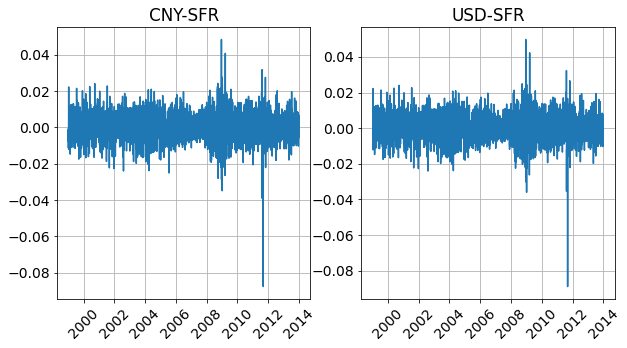
\includegraphics[width=0.7\textwidth]{figures/log_variation_exch}
%%\caption{Daily variation of CNY and USD exchange rates from January 1999 to December 2013 with respect to Swiss Franc.}
%%\label{fig:rate_variation}
%%\end{figure}
%
%To implement the linear regression model it can be used the \texttt{statsmodel} package. It is necessary to define the $X$ vector (i.e. the independent exchange rate variations) and $y$ (i.e. the target Yuan rate to SFR). Then add a constant to the model which represents the rate variation not correlated to other currency variations (i.e. $\alpha$).
%
%First, we fit the regression model for the period prior to July 2005 when the Chinese currency was pegged to the US dollar.
%
%\begin{ipython}
%import statsmodels.api as sm
%
%X = df.loc[df.index < '2005-06-30' ,
%           ['ret_YEN_SFR', 'ret_EUR_SFR',
%            'ret_GBP_SFR', 'ret_USD_SFR']]
%y = df.loc[df.index < '2005-06-30' ,'ret_CNY_SFR']
%X = sm.add_constant(X)
%
%est = sm.OLS(y, X).fit()
%print(est.summary())
%\end{ipython}
%\begin{ioutput}
%                            OLS Regression Results
%==============================================================================
%Dep. Variable:            ret_CNY_SFR   R-squared:                       1.000
%Model:                            OLS   Adj. R-squared:                  1.000
%Method:                 Least Squares   F-statistic:                 3.647e+06
%Date:                Tue, 08 Nov 2022   Prob (F-statistic):               0.00
%Time:                        13:46:53   Log-Likelihood:                 13749.
%No. Observations:                1692   AIC:                        -2.749e+04
%Df Residuals:                    1687   BIC:                        -2.746e+04
%Df Model:                           4
%Covariance Type:            nonrobust
%===============================================================================
%                  coef    std err          t      P>|t|      [0.025      0.975]
%-------------------------------------------------------------------------------
%const       -1.921e-07   1.74e-06     -0.110      0.912   -3.61e-06    3.23e-06
%ret_YEN_SFR    -0.0001      0.000     -0.477      0.633      -0.001       0.000
%ret_EUR_SFR    -0.0003      0.001     -0.379      0.705      -0.002       0.001
%ret_GBP_SFR    -0.0001      0.000     -0.224      0.823      -0.001       0.001
%ret_USD_SFR     1.0002      0.000   2545.320      0.000       0.999       1.001
%==============================================================================
%Omnibus:                      758.491   Durbin-Watson:                   2.824
%Prob(Omnibus):                  0.000   Jarque-Bera (JB):           889538.472
%Skew:                           0.456   Prob(JB):                         0.00
%Kurtosis:                     115.324   Cond. No.                         486.
%==============================================================================
%\end{ioutput}
%
%The most interesting (for us) part of the summary is:
%\begin{itemize}
%\item R-squared: the closer to 1 the higher is the linear correlation between $y$ and $X$;
%\item coef: the estimate of this model parameter (the weight assigned to this feature);
%\item std err: the standard error of our estimate. From these two values we can compute the t-score of our estimate:
%\begin{equation*}
%t = \frac{\textrm{coeff}}{\textrm{std err}}
%\end{equation*}
%which we can find on the third column ($t$);
%\item t: this value essentially provides us with a metric of how small the error is with respect to the estimated value: the larger the t-score, the smaller the error and the more confident we can be in our estimate.
%\item P>|t|: to better quantify our confidence, it’s usual to compute the p-value associated to the t-score. Under relatively common assumptions, we expect the t-score to follow a standard distribution and the probability of obtaining results at least as extreme as the value observed is simply the area under the curve to the right of the t-score value. This area is known as the p-value.
%There are some nuances to interpreting p-values but briefly, the smaller the p-value, the stronger the evidence that the value we’re estimating is different than zero (if the coefficient of a given feature is indistinguishable from zero then that feature is not relevant for our model).
%
%Typical thresholds for the p-value are:
%\begin{itemize}
%	\item $p<0.05$: moderate evidence;
%	\item $p<0.01$: strong evidence;
%	\item $p<0.001$: very strong evidence.
%\end{itemize}
%\end{itemize}
%
%In our example R-squared is 1, and the only largely significant predictor is USD (p-value 0) confirming that indeed CNY was anchored to US dollar prior July 2005.
%
%Second, we fit the regression model for the first six months following the announcement of the change in currency policy.
%
%\begin{ipython}
%X = df.loc[(df.index > '2005-07-01') & (df.index < '2005-12-31'),
%           ['ret_YEN_SFR', 'ret_EUR_SFR',
%            'ret_GBP_SFR', 'ret_USD_SFR',
%            'ret_WON_SFR', 'ret_MYR_SFR',
%            'ret_THB_SFR']]
%y = df.loc[(df.index > '2005-07-01') & (df.index < '2005-12-31'),
%           'ret_CNY_SFR']
%
%X = sm.add_constant(X)
%est = sm.OLS(y, X).fit()
%print(est.summary())
%\end{ipython}
%\begin{ioutput}
%                            OLS Regression Results
%==============================================================================
%Dep. Variable:            ret_CNY_SFR   R-squared:                       0.949
%Model:                            OLS   Adj. R-squared:                  0.946
%Method:                 Least Squares   F-statistic:                     326.3
%Date:                Tue, 08 Nov 2022   Prob (F-statistic):           8.41e-76
%Time:                        13:53:28   Log-Likelihood:                 667.58
%No. Observations:                 130   AIC:                            -1319.
%Df Residuals:                     122   BIC:                            -1296.
%Df Model:                           7
%Covariance Type:            nonrobust
%===============================================================================
%                  coef    std err          t      P>|t|      [0.025      0.975]
%-------------------------------------------------------------------------------
%const          -0.0001      0.000     -0.920      0.359      -0.000       0.000
%ret_YEN_SFR    -0.0097      0.037     -0.262      0.794      -0.083       0.063
%ret_EUR_SFR     0.0583      0.092      0.636      0.526      -0.123       0.240
%ret_GBP_SFR    -0.0306      0.044     -0.688      0.493      -0.119       0.057
%ret_USD_SFR     0.2122      0.148      1.433      0.154      -0.081       0.505
%ret_WON_SFR     0.1790      0.036      5.041      0.000       0.109       0.249
%ret_MYR_SFR     0.7373      0.142      5.178      0.000       0.455       1.019
%ret_THB_SFR    -0.0655      0.059     -1.110      0.269      -0.182       0.051
%==============================================================================
%Omnibus:                      195.464   Durbin-Watson:                   2.331
%Prob(Omnibus):                  0.000   Jarque-Bera (JB):            15756.757
%Skew:                          -5.874   Prob(JB):                         0.00
%Kurtosis:                      55.639   Cond. No.                     1.57e+03
%==============================================================================
%\end{ioutput}
%
%R-squared is quite close to 1 so there is some correlation between $y$ and $X$.
%During this six-month period, there is evidence of the Yuan departing from a US Dollar peg. The exchange rates with the statistically significant regression parameters (lowest p-values) are for the Korean Won (WON) and the Malaysian Ringgit (MYR).
%
%Similar regressions can be performed to examine for further changes in the implicit reference basket from 2006 through 2013.
%
%Finally it is possible to measure the annualized trend in the Yuan exchange rate relative to the other currencies in the studied period. The annualization is performed on the $\alpha$ coefficient which is the only one not related to other currency variations (i.e. the idiosyncratic part of the rate variation).
%
%\begin{ipython}
%print (f"{(1+est.params[0])**126-1:.4f}")
%\end{ipython}
%\begin{ioutput}
%-0.0150
%\end{ioutput}
%\noindent
%So the Yuan depreciated in the studied period.

\section{Capital Asset Pricing Model}
\label{sec:capm}

The Capital Asset Pricing Model (CAPM) describes the relationship between asset expected returns and \emph{systematic risk} of the market. No measure of unsystematic risk appears in the risk premium for in the world of CAPM diversification has already eliminated it.

Sharpe~\cite{bib:capm_sharpe} and Lintner~\cite{bib:capm_lintner} developed the Capital Asset Pricing Model whose central insight is that the riskiness of an asset is not measured by the standard deviation of its return but by its beta. In particular, there is a linear relationship between the expected return of any security (or portfolio) and the expected return of the market portfolio. It is given by

\begin{equation}
r_i = r_f + \beta_i(r_m-r_f)
\label{eq:capm}
\end{equation}
where:
\begin{itemize}
\item $r_i$ is the expected return of the $i^{th}$ security;
\item $r_f$ is the risk-free rate with zero standard deviation (e.g. risk-free asset includes Treasury Bills as they are backed by the U.S. government);
\item $r_m - r_f$ is the risk premium, $r_m$ denotes the market return including all securities in the market, whose proxy can be an index like SP500;
\item $\beta_i$ is a measure of $i^{th}$ asset volatility in relation to the overall market. $\beta$ is used in the CAPM to describe the relationship between market risk, and expected return.
\end{itemize}

The relationship between risk ($\beta$) and expected return is called \emph{Security Market Line} (SML). An example of this line is shown in Fig.~\ref{fig:sml}.

In the freely competitive financial markets described by CAPM, no security can sell for long at prices low enough to yield more than its appropriate return on the SML (\emph{undervalued} asset). The security would then be very attractive compared with other securities of similar risk, and investors would bid its price up until its expected return fell to the appropriate position on the SML. Conversely, investors would sell off any stock selling at a price high enough to put its expected return below its appropriate position (\emph{overvalued} asset). The resulting reduction in price would continue until the stock’s expected return rose to the level justified by its systematic risk.

\begin{figure}[htb]
	\centering
	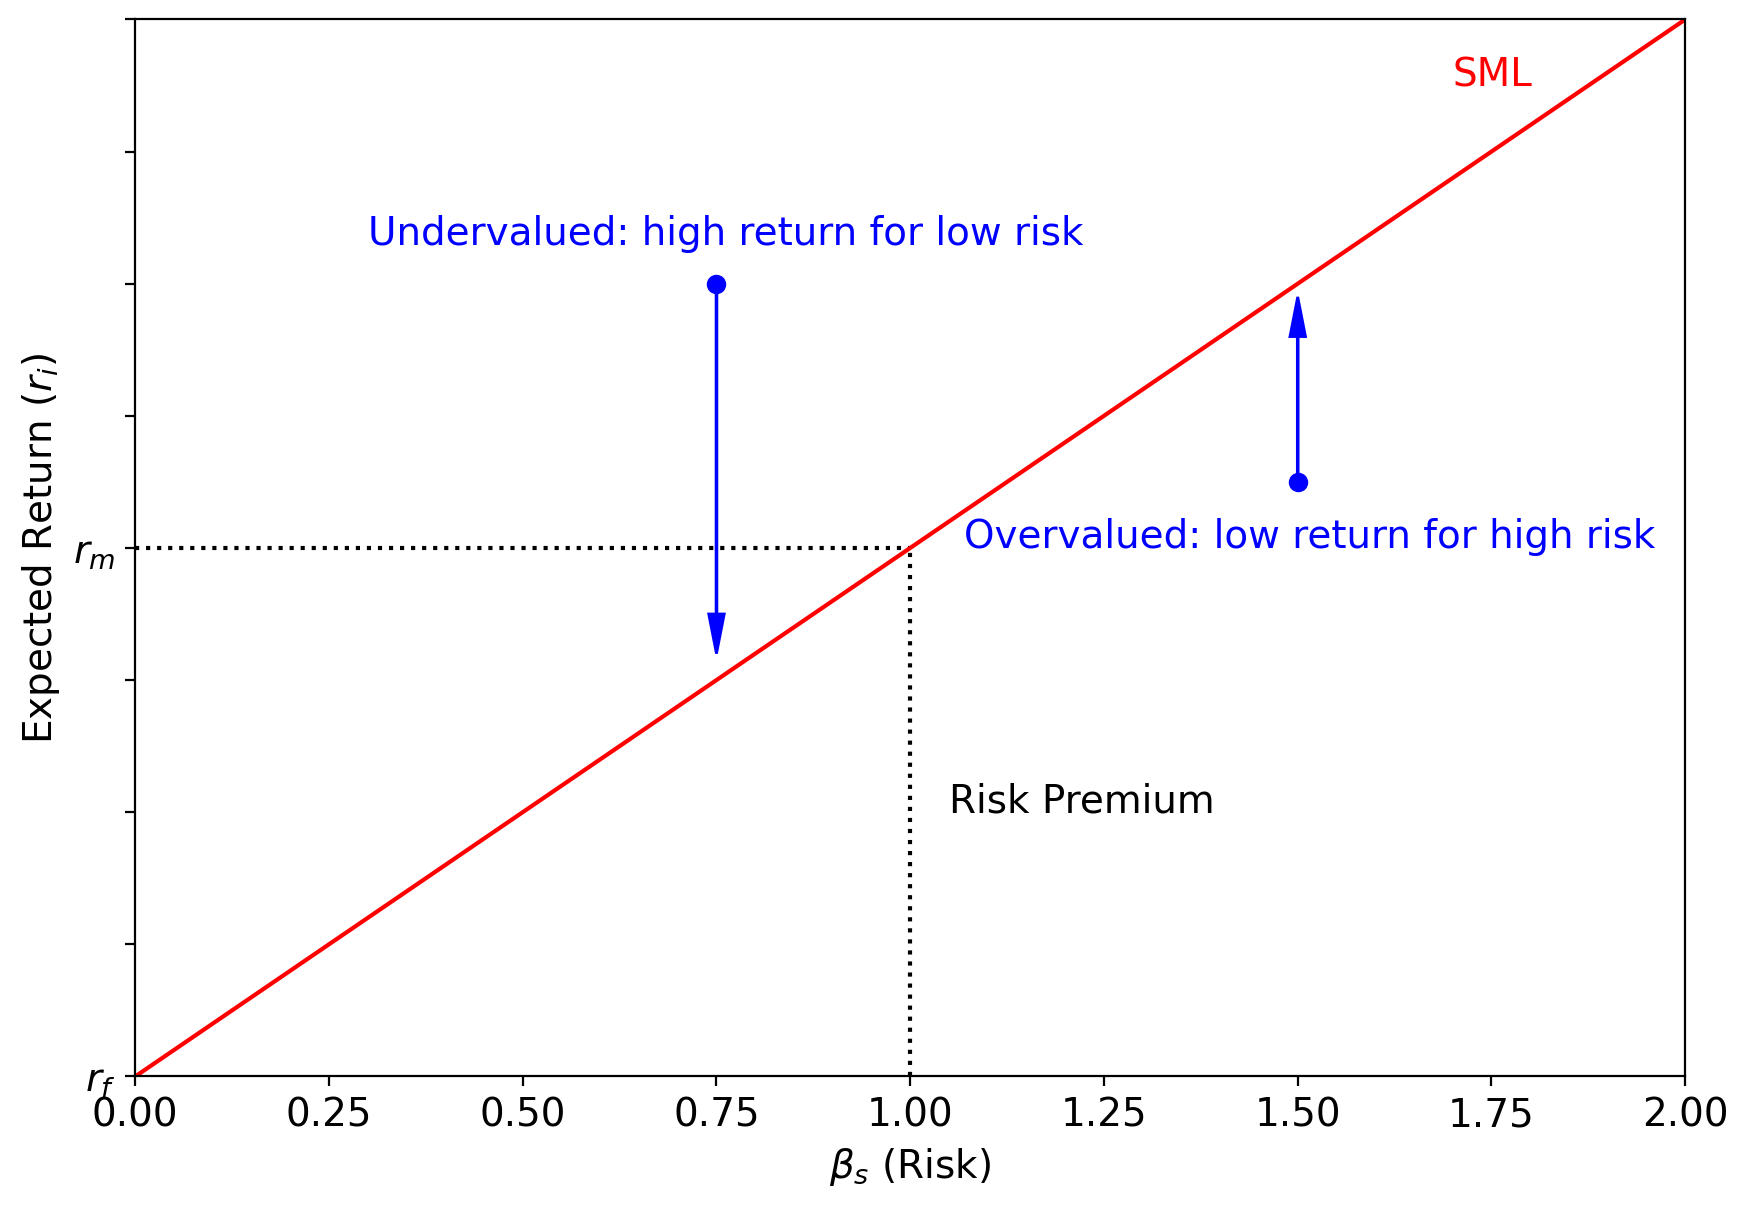
\includegraphics[width=0.7\textwidth]{figures/sml}
	\caption{Security market line.}
	\label{fig:sml}
\end{figure}

The key point in CAPM is the determination of $\beta$. This can be achieved with the measurement of the \emph{regression line} slope, in the market vs individual stock return plot.

\subsection{Regression in CAPM}

The regressed coefficient estimates can be expressed as

\begin{equation}
\beta \approx \cfrac{\text{Cov}(X,y)}{\text{Var}(X)}
\end{equation}

In the case of CAPM the line estimates the stock returns $y$ given the global market returns $X$ and so provides insights about how \emph{volatile}, or how risky, a stock is relative to the rest of the market.

In CAPM $\beta$ calculation is used to help investors understand whether a stock moves in the same direction as the rest of the market but for it to provide any useful clue, the market proxy should be related to the stock.

If $\beta$ of an individual stock = 1.0, means its price is perfectly correlated with the market, if $\beta < 1.0$, which is referred to as "defensive", indicates the security is theoretically less volatile than the market (provides lower returns, so it is less risky), while if $\beta > 1.0$, or "aggressive", indicates the assets price is more volatile than the market.

Those who use CAPM pick individual stocks or portfolios, and compare them to different indexes. The point is to find stocks that have high $\beta$, and portfolios that have high $\alpha$. High $\beta$ means the stock fares better than index with positive market and performs worse for negative market (contrary low $\beta$ gives lower performance for positive market and "better" returns in negative market), so those stocks have a chance at beating the market. $\alpha$ values above zero mean that a portfolio outperforms the market whatever it does.

\subsection{CAPM Example}
\label{sec:linear_regression}

Let's apply CAPM model to a couple of securities, the market proxy is the SP500 index while the risk free rate is approximated by the 3 months Treasury rate.
Input data can be downloaded with \href{https://raw.githubusercontent.com/matteosan1/finance_course/develop/libro/input_files/capm.csv}{capm.csv}.

Consider the General Electrics (GE) stock and apply CAPM to the series of its returns. Figure~\ref{fig:ge_returns} reports the historical series of closing price for GE and SP500.

\begin{figure}[htbp]
\centering
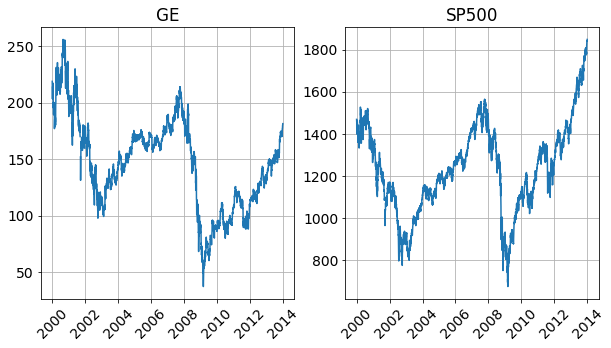
\includegraphics[width=0.7\textwidth]{figures/capm_ge}
\caption{Historical series of closing price for General Electrics stock (left) and SP500 (right).}
\label{fig:ge_returns}
\end{figure}

To implement the linear regression model it can be used the \texttt{statsmodel} package. It is necessary to define the $X$ vector (i.e. the independent exchange rate variations) and $y$ (i.e. the target Yuan rate to SFR). Then add a constant to the model which represents the rate variation not correlated to other currency variations (i.e. $\alpha$).

So to determine $\beta$ and $\alpha$ for GE stock the model is made of its excess of returns ($y$) and market excess of returns ($X)$

\pythoncodenon{code/linear_models_capm.py}

\begin{ioutput}
OLS Regression Results
===========================================================================
Dep. Variable:                 ret_GE   R-squared :                   0.572
Model:                            OLS   Adj. R-squared :              0.572
Method:                 Least Squares   F-statistic:                  4469.
Date:                Thu, 17 Nov 2022   Prob (F-statistic):            0.00
Time:                        08:51:58   Log-Likelihood:              9655.8
No. Observations:                3340   AIC:                     -1.931e+04
Df Residuals:                    3339   BIC:                     -1.930e+04
Df Model:                           1
Covariance Type:            nonrobust
===========================================================================
coef          std err          t      P>|t|      [0.025      0.975]
---------------------------------------------------------------------------
ret_SP500      1.1867      0.018     66.854      0.000       1.152    1.222
===========================================================================
Omnibus:                      900.145   Durbin-Watson:                1.973
Prob(Omnibus):                  0.000   Jarque-Bera (JB):         66833.895
Skew:                           0.275   Prob(JB):                      0.00
Kurtosis:                      24.908   Cond. No.                      1.00
===========================================================================
\end{ioutput}

The most interesting (for us) part of the summary is:
\begin{itemize}
\item R-squared: the closer to 1 the higher is the linear correlation between $y$ and $X$;
\item coef: the estimate of this model parameter (the weight assigned to this feature);
\item std err: the standard error of our estimate. From these two values we can compute the t-score of our estimate:
\begin{equation*}
t = \frac{\text{coeff}}{\text{std err}}
\end{equation*}
which we can find on the third column ($t$);
\item t: this value essentially provides us with a metric of how small the error is with respect to the estimated value: the larger the t-score, the smaller the error and the more confident we can be in our estimate.
\item P>|t|: to better quantify our confidence, it’s usual to compute the p-value associated to the t-score. Under relatively common assumptions, we expect the t-score to follow a standard distribution and the probability of obtaining results at least as extreme as the value observed is simply the area under the curve to the right of the t-score value. This area is known as the p-value.
There are some nuances to interpreting p-values but briefly, the smaller the p-value, the stronger the evidence that the value we’re estimating is different than zero (if the coefficient of a given feature is indistinguishable from zero then that feature is not relevant for our model).

Typical thresholds for the p-value are:
\begin{itemize}
	\item $p<0.05$: moderate evidence;
	\item $p<0.01$: strong evidence;
	\item $p<0.001$: very strong evidence.
\end{itemize}
\end{itemize}

From the summary results that $\beta$ is statistically significant and equal to 1.187. Fig.~\ref{fig:capm_fit} reports the dataset and the linear regression fit.

\begin{figure}[htbp]
\centering
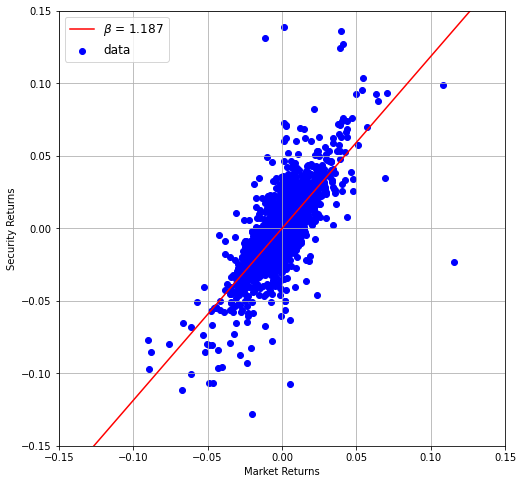
\includegraphics[width=0.7\textwidth]{figures/capm_fit}
\caption{Linear regression of market return vs stock return for GE security.}
\label{fig:capm_fit}
\end{figure}

If you imagine to have a portfolio, and that we have the $\beta$s of each individual stock to apply CAPM it is enough to perform a weighted sum of the expected return according to the model of each stock.

\subsection{Criticism to CAPM}
As we have seen the whole model is about plotting a line in a scatter plot, it’s not a very complex model. Assumptions under the model are even more simplistic. For example:
\begin{itemize}
\tightlist
\item expect that all investors are rational and they avoid risk;
\item everyone have full information about the market;
\item everyone have similar investment horizons and expectations about future movements;
\item stocks are all correctly priced.
\end{itemize}

Moreover, this is a model from the 1960s. Market dynamics were different back then. And of course, this is a retrospective model. We cannot know how future stock prices move and how the market behaves.
Interesting extension of CAPM involves \emph{Bayesian regression}\cite{bib:bayesian_regression} but it will not be discussed here.

\section{Normal Returns Hypothesis}

In finance, returns are almost always modelled with a \textbf{Normal distribution}: 
\begin{itemize}
	\item \emph{Markowitz Theory} (normally distributed single asset returns $R = (R_1, R_2, \dots, R_n)^T$ implies normal distribution for $R_p \sim \mathcal{N}(\mu_p, \sigma_p^2)$, the normal distribution is fully characterized by mean ($\mu$) and variance ($\sigma^2$), so those are the only two parameters an investor should consider);
	\item \emph{CAPM} (if returns wouldn't be normally distributed the relation between $R_i$ and $R_M$ couldn't be linear making the simple regression model useless or ar least incomplete, in a multivariate normal distribution the correlation is fully determined by the covariance matrix, hence $\beta_i = \frac{\cov(R_i, R_M)}{\var(R_M)}$ measure completely each asset contribution to risk).
\end{itemize} 

However, empirical observations of the historical series shows a systematic violation of this assumption and the major limitations of Gaussian models are:
\begin{enumerate}
	\item \textbf{Skewness}: equity returns often show a negative asymmetry: negative market shocks (\textit{crashes}) are stringer and happens more frequently than equally strength rallies;
	\item \textbf{Kurtosis \& Fat Tails}: return distribution is leptocurtic (high kurtosis), meaning that extreme events have higher probability to happen than the Gaussian distribution predicts;
	\item \textbf{Non-linear dependence}: during financial stressed periods, asset correlation increases (\textit{contagion}). The standard Pearson correlation is not able to catch the tail dependence.
\end{enumerate}

To check the actual return distribution we can \textbf{fit} the historical series distribution with Gaussian and other functions (e.g. t-student, a bell-like shaped distribution with fatter tails).

\begin{finmarkets}
	\label{sec:how_to_fit}
	Histogram fitting is the art of choosing a probability model for the unknown population, and calibrating that model (setting the best value for the model parameters) using a representative sample from the population.
	
	In \texttt{python} this can be done quite easily since each \texttt{scipy.stats} distribution has a convenient method \texttt{fit} which performs the calibration and return an array with the best estimate of the parameter values.
\end{finmarkets}

\begin{ipythonnon}
import pandas as pd

from scipy.stats import t, norm

df = pd.read_csv("bmw_siemens.csv", index_col="Date")
df = df.dropna()

bmw = df['BMW.DE']
sie = df['SIE.DE']

bmw_norm = norm.fit(bmw)
sie_norm = norm.fit(sie)

bmw_f2 = norm(loc=bmw_norm[0], scale=bmw_norm[1])
sie_f2 = norm(loc=sie_norm[0], scale=sie_norm[1])

bmw_fit = t.fit(bmw)
sie_fit = t.fit(sie)

bmw_f = t(*bmw_fit)
sie_f = t(df=sie_fit[0], loc=sie_fit[1], scale=sie_fit[2])
\end{ipythonnon}

Figure~\ref{fig:bmw_siemens_returns} clearly shows the superior agreement in the t-student fit, confirming that the Normal hypothesis is a too crude approximation.

\begin{figure}[htbp]
	\centering
	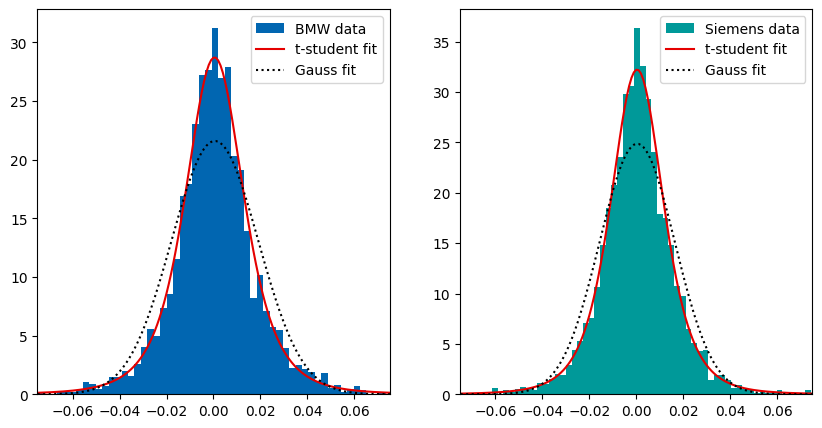
\includegraphics[width=0.7\textwidth]{figures/bmw_siemens_v2}
	\caption{Gaussian and t-student fit to BMW and Siemens historical series of returns.}
	\label{fig:bmw_siemens_returns}
\end{figure}

To give a more quantitative result though, we can perform the \textit{Jarque-Bera Test}. Given a sample of returns $R_1, R_2, \dots, R_T$ with mean $\mu$ and standard deviation $\sigma$, the Jarque-Bera Test check formally the null hypothesis $H_0$ that the sample comes from a Normal distribution, comparing simultaneously skewness and Kurtosis excess:

$$JB = \frac{T}{6} \left( S^2 + \frac{(K - 3)^2}{4} \right) \sim \chi^2(2)$$
Under $H_0$, the $JB$ statistic follows a Chi-2 distribution with 2 dof. If the $p\text{-value} < 0.05$, $H_0$ is rejected: returns are NOT Gaussian.

\begin{ipythonnon}
import scipy

def JarqueBeraTest(df: pd.DataFrame) -> pd.DataFrame:
  results = []
  n_obs = len(df)

  for col in df.columns:
    series = df[col]
    skewness = float(scipy.stats.skew(series))
    kurtosis = float(scipy.stats.kurtosis(series, fisher=False))
    jb_stat, p_value = scipy.stats.jarque_bera(series)

    results.append({"Asset": col, "Obs": n_obs, "Skewness": skewness,
                    "Kurtosis": kurtosis, "JB Statistic": jb_stat,
	                "P-Value": p_value, "Is Normal": bool(p_value > 0.05)})

  return pd.DataFrame(results).set_index("Asset")

print (JarqueBeraTest(df))
\end{ipythonnon}
\begin{ioutput}
         Obs  Skewness  Kurtosis  JB Statistic  P-Value  Is Normal
Asset
BMW.DE  3252 -0.033995  7.563353   2822.303924      0.0      False
SIE.DE  3252  0.058003  8.167413   3619.966069      0.0      False
\end{ioutput}

\section{Multifactor Models}

In its original formulation the Capital Asset Pricing Model (CAPM) treats the market return as the only factor. Nevertheless a stock’s return can depend also on other macro-economic factors, such commodity prices, interest rates, economic growth (GDP). In this case we talk about \emph{multifactor models} which can be used for: return forecasting, risk modeling, transaction cost analysis, and performance attribution.
By decomposing asset returns into different components (\emph{factors}), allows a better understanding of the sources of portfolio return and risk.

Factor models are based on the idea that security returns consist of two components:
\begin{itemize}
\tightlist
\item the part that is driven by a set of common factors;
\item and the part unexplained by these factors hence idiosyncratic in nature.
\end{itemize}
\begin{equation}
r_{t} = \sum_{k=1}^{K} X_{kt} f_{kt} + \epsilon_{t} = \mathbf{Xf} + \boldsymbol{\epsilon}
\label{eq:multifactor}
\end{equation}
where: $r_{t}$ is the security return over period $t$, $X_{kt}$ its \emph{exposure} to k$^{th}$ factor at the beginning of period $t$, $f_{kt}$ is the \emph{factor return} to k$^{th}$ factor over period $t$ and $\epsilon_{t}$ is the residual return over period $t$ (i.e. there are $K$ factors, and $T$ time periods).

\subsection{Types of Factor Models}

In practice, there are three common classes of factor models depending on the statistical techniques used to estimate factor returns and/or factor exposures.

\begin{center}
\scriptsize
\begin{tabularx}{\linewidth}{>{\hsize=.3\hsize}X>{\hsize=.4\hsize}X>{\hsize=.4\hsize}X>{\hsize=.5\hsize}X>{\arraybackslash}X}
Type & Inputs & Outputs & Estimation Method & \textcolor{ansi-green}{Adv.}/\textcolor{ansi-red}{Disadv.} \\
\toprule
Explicit & security returns, factor returns & factor exposures &\begin{tabular}[t]{@{}l@{}}time-series\\ regression\end{tabular}
& \textcolor{ansi-green}{Accommodates any time series as factors, linked to macroeconomic fundamentals.}
\textcolor{ansi-red}{Possible non-intuitive factor exposures.} \\
\midrule
Implicit & security returns, factor exposures & factor returns &\begin{tabular}[t]{@{}l@{}}cross-sectional\\ regression\end{tabular} & \textcolor{ansi-green}{Intuitive exposures linked to asset characteristics, incorporates security fundamental data, responsive to asset characteristics changes.} \textcolor{ansi-red}{Data intensive.} \\
\midrule
Statistical & security returns, factor exposures & factor returns &\begin{tabular}[t]{@{}l@{}}principal component\\analysis\end{tabular} & \textcolor{ansi-green}{Requires only asset-level price data, might capture new risk sources, relatively easy to build.} \textcolor{ansi-red}{Lack of interpretability.} \\
\end{tabularx}
\end{center}
\normalsize

\subsection{Risk Decomposition and Estimation with Factor Models}

Once factor exposures are calculated, one can carry out risk decomposition and forecast at both the individual security and the aggregate portfolio levels.

Let $R_P$ denote the return of some portfolio $P$ over period $t$
\begin{equation}
R_P = \mathbf{w}_P^T \mathbf{r}
\label{eq:portfolio_return}
\end{equation}
where $\mathbf{w}_P$ are the portfolio weights and $\mathbf{r}$ denotes the vector of security returns.

Substituting~\ref{eq:multifactor} into Eq.~\ref{eq:portfolio_return} gives
\begin{equation}
R_P = \mathbf{w}^T_P \mathbf{Xf} + \mathbf{w}^T_P\boldsymbol{\epsilon}
\end{equation}
where $\mathbf{X}$ is a $N\times K$ matrix specifying each security’s exposures to each model factors ($\mathbf{f}$).

The risk $\sigma_P$ of the portfolio can be decomposed into the factor and the idiosyncratic components:
\begin{equation}
\sigma^2_P = \mathbf{w}_P^T\mathbf{\Omega}\mathbf{w}_P = \mathbf{w}_P^T \mathbf{XFX}^T \mathbf{w}_P + \mathbf{w}_P^T \mathbf{\Delta} \mathbf{w}_P
\end{equation}

$\mathbf{\Omega}$ represents the $N \times N$ asset covariance matrix that without a factor model the calculation of $\mathbf{\Omega}$ would involve computing the pairwise sample covariance for each element in the matrix (e.g. $N$ is usually very large, hundreds of assets, relative to the number of time periods $T$ of the return time series, which makes the estimated covariance matrix unstable and ill-conditioned).

The factor model framework allows to reduce the dimensionality of the problem significantly. In this approach, we can express the asset covariance matrix in terms of factor model ingredients:
\begin{equation}
\mathbf{\Omega} = \mathbf{XFX}^T + \mathbf{\Delta}
\end{equation}
where $\mathbf{X}$ is the factor exposure matrix, $\mathbf{F}$ is the $K\times K$ factor covariance matrix, and $\mathbf{\Delta}$ is the $N\times N$ idiosyncratic covariance matrix (which is usually assumed to be diagonal).

\subsubsection{Example}

Consider the example of previous Section and improve the model by adding the crude oil price as a second factor. Perform again the linear regression

\pythoncodenon{code/linear_models_multifactor.py}

\begin{ioutput}
OLS Regression Results
==============================================================================
Dep. Variable:                 ret_GE   R-squared (uncentered):          0.574
Model:                            OLS   Adj. R-squared (uncentered):     0.574
Method:                 Least Squares   F-statistic:                     2251.
Date:                Thu, 17 Nov 2022   Prob (F-statistic):               0.00
Time:                        09:05:11   Log-Likelihood:                 9662.9
No. Observations:                3340   AIC:                        -1.932e+04
Df Residuals:                    3338   BIC:                        -1.931e+04
Df Model:                           2
Covariance Type:            nonrobust
==============================================================================
coef          std err          t      P>|t|      [0.025      0.975]
------------------------------------------------------------------------------
ret_SP500      1.2004      0.018     66.376      0.000       1.165       1.236
ret_Brent     -0.0371      0.010     -3.768      0.000      -0.056      -0.018
==============================================================================
Omnibus:                      878.756   Durbin-Watson:                   1.974
Prob(Omnibus):                  0.000   Jarque-Bera (JB):            63119.110
Skew:                           0.231   Prob(JB):                         0.00
Kurtosis:                      24.292   Cond. No.                         1.90
==============================================================================
\end{ioutput}

The regression coefficient for the oil factor (ret\_Brent) is statistically significant and negative. Over the analysis period, price changes in GE stock are negatively related to the price changes in oil.
Let's apply the same model now to Exxon (XOM) stock.

\begin{ioutput}
OLS Regression Results
==============================================================================
Dep. Variable:                ret_XOM   R-squared (uncentered):          0.549
Model:                            OLS   Adj. R-squared (uncentered):     0.549
Method:                 Least Squares   F-statistic:                     2031.
Date:                Thu, 17 Nov 2022   Prob (F-statistic):               0.00
Time:                        09:07:25   Log-Likelihood:                 10402.
No. Observations:                3340   AIC:                        -2.080e+04
Df Residuals:                    3338   BIC:                        -2.079e+04
Df Model:                           2
Covariance Type:            nonrobust
==============================================================================
coef          std err          t      P>|t|      [0.025      0.975]
------------------------------------------------------------------------------
ret_SP500      0.8129      0.014     56.082      0.000       0.785       0.841
ret_Brent      0.1453      0.008     18.391      0.000       0.130       0.161
==============================================================================
Omnibus:                      477.069   Durbin-Watson:                   2.075
Prob(Omnibus):                  0.000   Jarque-Bera (JB):             6852.309
Skew:                           0.036   Prob(JB):                         0.00
Kurtosis:                      10.017   Cond. No.                         1.90
==============================================================================
\end{ioutput}

The R-squared for XOM is slightly lower than for GE. Its relationship to the market index is less strong (lower t value).
The regression coefficient for the oil factor (ret\_Brent) is statistically significant and, unlike GE, positive.

\subsection{Fama-French Three-Factor Model}
This model was proposed in 1993 by Eugene Fama and Kenneth French to describe stock returns~\cite{bib:fama_french}. The three-factor model is
\begin{equation}
r=\alpha + \beta_m \textrm{MKT} +\beta_s \textrm{SMB}+ \beta_h \textrm{HML}
\end{equation}
where
\begin{itemize}
\tightlist
\item MKT: is the excess return of the market (e.g. the value-weighted return of all firms listed on the NYSE, AMEX, or NASDAQ minus the 1-month Treasury Bill rate);
\item SMB (Small Minus Big): measures the excess return of stocks with small market cap over those with larger market cap;
\item HML (High Minus Low): measures the excess return of value stocks over growth stocks. Value stocks have high book to price ratio (B/P) than growth stocks.
\end{itemize}

This setting represents the original Fama-French model. This very same approach has been also extended with the Fama-French Five-Factor model which comprises two more factors:
\begin{itemize}
\tightlist
\item RMW (Robust Minus Weak): measures the excess returns of firms with high operating profit margins over those with lower profits;
\item CMA (Conservative Minus Aggressive): measures the excess returns of firms investing less over those investing more.
\end{itemize}
Finally, momentum is another commonly used factor. It captures excess returns of stocks with highest returns over those with lowest returns.

The application of such models goes along the lines of the CAPM with the only difference being the calculation of a multidimensional regression.

%* The Fama and French model has three factors:
%* the size of firms (**SMB**, small minus big),
%* book-to-market values (**HML**, high minus low),
%* **excess return on the market** (portfolio's return less the risk-free rate of return).
%
%* SMB accounts for publicly traded companies with small market caps that generate higher returns, while HML accounts for value stocks with high book-to-market ratios that generate higher returns in comparison to the market.
%
%* Represent each characteristic of interest ($f_k(t)$) by a portfolio:
%1. sort all assets by that characteristic;
%2. build the portfolio by going long the top quantile of assets and short the bottom quantile.
%
%* **The factor corresponding to this characteristic is the return on this portfolio**.
%* The $X_{nk}(t)$ are estimated for each asset $n$ by regressing over the historical values of $r_n(t)$ and of the factors.

\section{Principal Components Analysis}
\label{sec:pca}

\emph{Principal Component Analysis} (PCA), is a dimensionality-reduction method that is often used to reduce the complexity of large datasets, by transforming the original set of variables into a smaller one that still contains most of the information of the large set.

Reducing the number of variables of a dataset naturally comes at the expense of accuracy, but the trick in dimensionality reduction is to trade a little accuracy for simplicity.

So, to sum up, the idea of PCA is simple: reduce the number of variables of a dataset, while preserving as much information as possible.

\subsection{Principal Components}

Principal components are new variables that are constructed as linear combinations or mixtures of the original ones. These combinations are done in such a way that the new variables (i.e. principal components) are uncorrelated and most of the information within the initial variables is squeezed or compressed into the first components.

So, the idea is that a $n$-dimensional dataset gives you $n$ principal components, but PCA tries to put maximum possible information in the first component, then maximum remaining information in the second and so on.

Organizing information in principal components this way, will allow you to reduce dimensionality without losing much information, by discarding the components with low information and considering the remaining components as your new variables.

\emph{An important thing to realize here is that the principal components are less interpretable and don’t have any real meaning since they are constructed as linear combinations of the initial variables.}

Geometrically speaking, principal components represent the directions of the data that explain a maximal amount of variance, that is to say, the lines that capture most information of the data. The relationship between variance and information here, is that, the larger the variance carried by a line, the larger the dispersion of the data points along it, and the larger the dispersion along a line, the more the information it has.
%To put all this simply, just think of principal components as new axes that provide the best angle to see and evaluate the data, so that the differences between the observations are better visible.

\subsection{Step-by-Step Explanation}

Let's see how this kind of technique can be implemented starting from a multidimensional initial dataset
\begin{equation}
	X=\begin{bmatrix}
		x^{(1)}_1 &x^{(2)}_1&\cdots &x^{(m)}_1 \\
		x^{(1)}_2 &x^{(2)}_2&\cdots &x^{(m)}_2 \\
		\vdots &\vdots &\vdots &\vdots \\
		x^{(1)}_n &x^{(2)}_n&\cdots &x^{(m)}_n
	\end{bmatrix}
\end{equation}

For the sake of simplicity let's imagine that our sample is the two-dimensional one represented in the left graph of Fig.~\ref{fig:pca_dataset}.

\begin{figure}[htb]
	\centering
	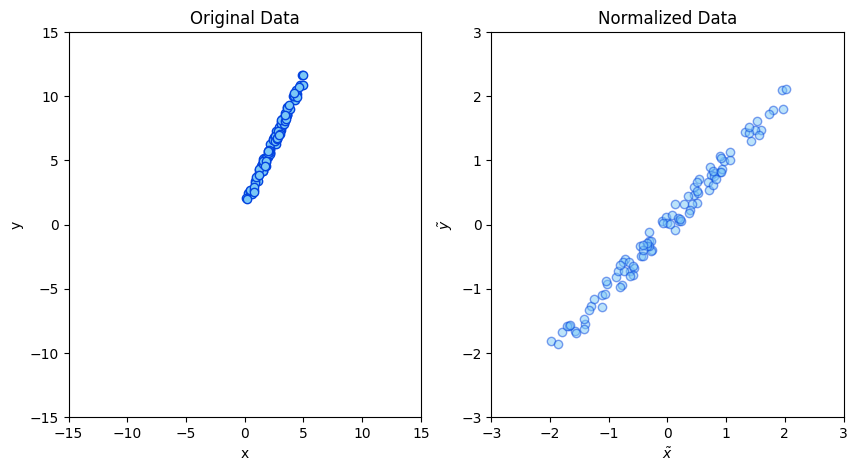
\includegraphics[width=0.9\linewidth]{figures/pca_raw_std_data.png}
	\caption{The dataset used in the PCA example (left), and the same dataset after \emph{normalization} (right).}
	\label{fig:pca_dataset}
\end{figure}

\subsubsection*{Step 1: Standardization}

The aim of this step is to standardize the range of the continuous initial variables so that each one of them contributes equally to the analysis.

More specifically, the reason why it is critical to perform standardization prior to PCA, is that the latter is quite sensitive regarding the variances of the initial variables. That is, if there are large differences between the ranges of initial variables, those variables with larger ranges will dominate over those with small ranges (for example, a variable that ranges between 0 and 100 will dominate over a variable that ranges between 0 and 1), which will lead to biased results. So, transforming the data to comparable scales can prevent this problem.

Mathematically, this can be done by subtracting the mean and dividing by the standard deviation for each value of each variable
\begin{equation*}
x' = \cfrac{x-\bar{x}}{\sigma_x}
\end{equation*}

Once the standardization is done, all the variables will be transformed to the same scale. Right plot of Fig.~\ref{fig:pca_dataset} shows the standardized dataset used in the following.

\subsubsection*{Step 2: Covariance Matrix Computation}

The aim of this step is to understand how the variables of the input dataset are varying from the mean with respect to each other, or in other words, to see if there is any relationship between them.

The covariance matrix is a symmetric $n\times n$ (where $n$ is the number of dimensions) that has as entries the covariances associated with all possible pairs of the initial variables. %Since the covariance of a variable with itself is its variance ($\textrm{cov}(a, a)= \textrm{var}(a)$), in the main diagonal (top-left to bottom-right) we actually have the variances of each initial variable. And since the covariance is commutative ($\textrm{cov}(a, b) = \textrm{cov}(b, a)$), the entries of the covariance matrix are symmetric with respect to diagonal.
Once we have centred our data around 0, $[X^T][X]$ is the covariance matrix.

\begin{equation}
	[\Sigma]=[X^T][X] =
	\begin{bmatrix}
		\var(x_1) & \cov(x_2, x_1) & \cdots & \cov(x_n, x_1) \\
		\cov(x_1, x_2) & \var(x_2) & \cdots & \cov(x_n, x_2) \\
		\vdots & \vdots & \vdots & \vdots \\
		\cov(x_1, x_n) & \cov(x_2, x_n) & \cdots & \var(x_n)
	\end{bmatrix}
\end{equation}

What do the covariances that we have as entries of the matrix tell us about the correlations between the variables ?
It’s actually the sign of the covariance that matters:
\begin{itemize}
	\item if positive then: the two variables increase or decrease together (correlated);
	\item if negative then: one increases when the other decreases (Inversely correlated).
\end{itemize}

\subsubsection*{Step 3: Compute the Eigenvectors and Eigenvalues of the Covariance Matrix to Identify the Principal Components}

It is possible to demonstrate that the eigenvectors of the covariance matrix are actually the directions of the axis where there is the most variance (i.e. most information) and that we call \emph{principal components}. Eigenvalues are simply the coefficients, attached to eigenvectors, which give the amount of variance carried in each principal component (see Sec.~\ref{eigenvectors-and-eigenvalues} for a description of eigenvectors-eigenvalues).

For our example the eigenvectors are defined as
\begin{ioutput}
        PC1       PC2
x  0.707107  0.707107
y  0.707107 -0.707107
\end{ioutput}
with the following eigenvalues (normalized to 1)
\begin{ioutput}
array([0.99662716, 0.00337284])
\end{ioutput}

According to these results PC1 and PC2 carry respectively 99.7\% and 0.3\% of the variance of the data.

\subsubsection*{Step 4: Create a Feature Vector}

In this step, what we do is, to choose whether to keep all these components or discard those of lesser significance (of low eigenvalues), and form with the remaining ones a matrix of vectors that we call \emph{feature vector}.

So, the feature vector is simply a matrix that has as columns the eigenvectors of the components that we decide to keep. This makes it the first step towards dimensionality reduction, because if we choose to keep only $p$ eigenvectors (components) out of $n$, the final data set will have only $p$ dimensions.

Continuing with the example from the previous step, we can either form a feature vector with both of the eigenvectors $v1$ and $v2$, or discard the eigenvector $v_2$, which is the one of lesser significance, and form a feature vector with $v_1$ only.

Discarding the eigenvector $v_1$ will reduce dimensionality by 1, and will consequently cause a loss of information in the final data set. But given that $v_1$ was carrying only 0.3\% of the information, the loss will be therefore not important and we will still have 99.7\% of the information that is carried by $v_2$.

Figure~\ref{fig:pca_result} shows the two principal components.

\begin{figure}[hbt]
\centering
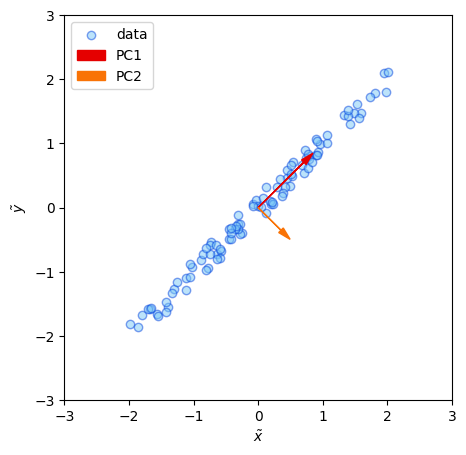
\includegraphics[width=0.5\linewidth]{figures/pca_pcs}
\caption{The directions corresponding to the first two principal components of our example dataset.}
\label{fig:pca_result}
\end{figure}

\subsubsection*{Step 5: Recast Data Along Principal Components}

At this point we can use the feature vector to re-orient data from the original axis to the ones represented by the principal components.
This can be done by multiplying the transpose of the original dataset by the transpose of the feature vector

\begin{equation}
[Y] = [X^T][F^T]
\end{equation}

The rotation transformed our dataset that have now the more variance on one of the Cartesian axis.
You could keep only this dimension and have a fairly good representation of the data. Figure~\ref{fig:pca_rotated} shows the effect of such a rotation to our sample.
%\clearpage
\begin{figure}[hbtp]
\centering
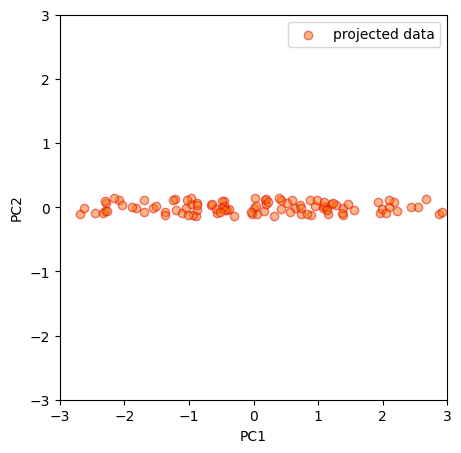
\includegraphics[width=0.5\linewidth]{figures/pca_projected_data}
\caption{The dataset rotated so that the usual Cartesian coordinates correspond to the first two principal components.}
\label{fig:pca_rotated}
\end{figure}

\subsection{Practical problems}
PCA is not invariant to scaling. Before applying PCA, we should consider whether or not to standardize the data $X$, besides removing of the mean from the data before applying PCA. In practice, it depends on the context of the data and the objective, but there are two general tips regarding this problem:
\begin{enumerate}
	\item If features are measured in different units that are not comparable, we should first standardize them before applying PCA.
	\item If features are measured in comparable units, then we can keep them unscaled to preserve the original variability information.
\end{enumerate}

Furthermore PCA can not be used if the data is not Gaussian. PCA is based on the assumption that the data is normally distributed, that is why we can represent all the information from the covariance. In the case of non-Gaussian data, independent component analysis (ICA) is often used.

\begin{finmarkets}
In the previous example and in the following the \texttt{PCAWrapper} class of the \texttt{finmarkets} module has been used.
This is a simple wrapper which implements the PCA algorithm and has few utility methods to get relevant information, e.g. extract components and project the data along the new axis.
\end{finmarkets}

\pythoncodenon{code/linear_models_pca.py}

\subsection{Term Structure Analysis Using PCA}

A bond’s yield is the interest income received by an investor from investing in debt securities. Bonds with a fixed coupon have an interest rate that accrues on the face value.
Current yield is the ratio of annual coupon payments to the current market value of the bond:
\begin{equation}
\text{Current Yield} = \cfrac{\text{Annual Coupon Payment}}{\text{Bond Price}}
\end{equation}

The yield curve represents the time structure of interest rates and shows the relationship between the yields of financial instruments and their maturity.

The Treasuries bond yield curve is not only used as a benchmark to assess the value of other debt instruments but is also considered one of the most important economic indicators to watch as a precursor to a future cyclical downturn in the US economy.

Usually, yields of longer-dated securities are higher than those of shorter-dated securities. Such a yield curve is considered \emph{normal} because the market usually requires more compensation for more risk under normal conditions. Long-term bonds are subject to greater risks, such as changes in interest rates and increased potential default risk.
However, the short-term yield sometimes exceeds the long-term yield, and the spread turns negative. The result is a \emph{concave} curve.

The \emph{inversion} (concavity) of the Treasuries curve in the US is considered one of the proxies for an imminent recession or downturn in the economy.

In the following example, we analyse the data of Treasury bonds between $1^{st}$ January 2017 and $31^{st}$ December 2018 taken using the Federal Reserve Bank of St. Louis API.
The US economy has been growing steadily in the period under review since after a rebound in 2016, it grew by 3.1\% in 2018 after climbing by 2.5\% in 2017.

The dateset is available \href{https://github.com/matteosan1/finance_course/raw/develop/input_files/DGS_2017_2018.csv"}{here}.

\subsection{Factor Model}
Let $X$ be the yield curve consisting of bonds of $p$ maturities with $N$ observations. We will model $X$ as a $k$ factor model.

The $k$ factor model for the yield curve $X$ can then be presented in the following way

\begin{equation}
X = \mu_ X + Zf + e
\end{equation}
\noindent
where $\mu_X = (\mu_1,\ldots, \mu_p)$ is the mean vector of $X$, $e = (e_1,\ldots, e_N )$ is the residuals and
\begin{equation}
Z =
\begin{bmatrix}
	z_{1,1} & z_{1,2} & \cdots & z_{1,k} \\
	z_{2,1} & z_{2,2} & \cdots & z_{2,k} \\
	\vdots & \vdots & \ddots & \vdots \\
	z_{N,1} & z_{N,2} & \cdots & z_{N,k} \\
\end{bmatrix}
\end{equation}
consist of $k$ factors,
\begin{equation}
f =
\begin{bmatrix}
	f_{1,1} & f_{1,2} & \cdots & f_{1,p} \\
	f_{2,1} & f_{2,2} & \cdots & f_{2,p} \\
	\vdots & \vdots & \ddots & \vdots \\
	f_{k,1} & f_{k,2} & \cdots & f_{k,p} \\
\end{bmatrix}
\end{equation}
the factor loading matrix; i.e., the observation $i$ of feature $j$ is

\begin{equation}
x_{i,j} = \mu_j + \sum_{l=1}^k z_{i,l}f_{l,j} + e_{i,j}
\end{equation}

The difference with the previous studies is that instead of identifying external factors, we will focus on self-contained independent drivers, i.e., factors related to the curve itself, such as slope and curvature.

Through this approach, we will recognize the key structure of the yield curve dynamics and will be able to answer how 2Y, 10Y, and 30Y bond yields move together. Moreover, PCA will help us to naturally reduce the dimensionality of the factors based on the coefficient of explained variance.

\subsection{PCA on Term Structure}

The yield/rate time series of different maturities are shown in the top plot of Fig.~\ref{fig:yield_rate_ts}. It is clear that all curves are moving in the same direction, which indicates the idea that some common factors drive the yield dynamic.

In bottom Fig.~\ref{fig:yield_rate_ts} we can see the yield curve term structure on different dates. In contrast to the previous figure, here one can distinctly see the inconsistencies in the dynamics and it is obvious that in some periods the movement is quite the opposite.

\begin{figure}[htb]
	\centering
	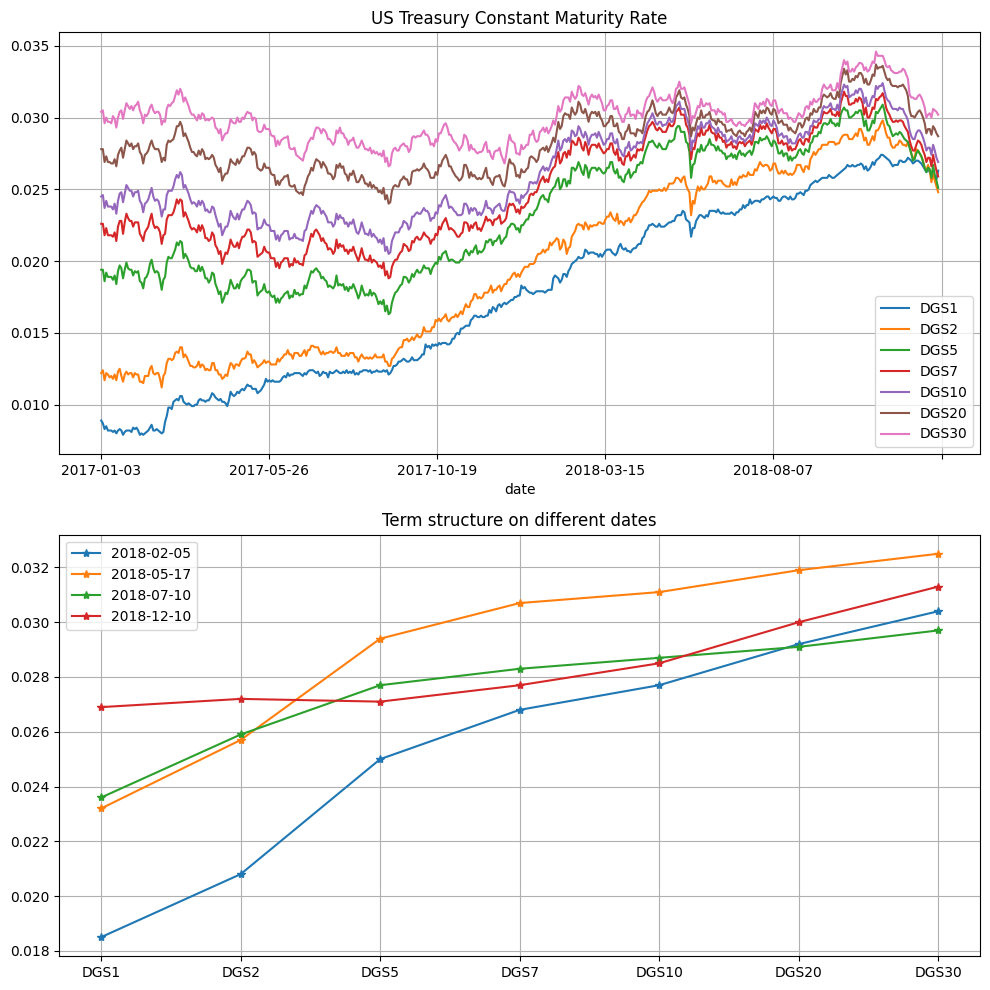
\includegraphics[width=0.7\linewidth]{figures/treasury_rate}
	\caption{Yield rate time series for different maturity Treasury bonds (top). Yield rate at different dates (bottom).}
	\label{fig:yield_rate_ts}
\end{figure}

Let us consider in more detail the different types of changes between the dates:
\begin{enumerate}
\item Level change: modifies the interest rates of all maturities in nearly equal amounts, inducing a parallel shift that changes the level of the entire yield curve. An example of level change can be seen by observing the green (2018-02-05) and orange (2018-05-17) curves. Both are moving in the same direction with almost identical slopes, and the only difference is the level: the green curve is shifted compared to the orange one.
\item Slope change: increases short-term interest rates by much more than long-term interest rates so that the yield curve becomes less abrupt and its slope decreases.
For example, from 2018-05-17 (orange) to 2018-12-10 (pink), the slope of the curve changed as the short-term yield increased while the long-term yield decreased (DGS2 to DGS5).
\item Curvature change: reflects how the difference between the medium-long-term premium (i.e., the long-term minus the medium-term rate level) and the short-medium-term premium (i.e., the medium-term minus the short-term rate level) changes from each day. In other words, the ”belly” of the curve shifts relatively to variations in short-term and long-term levels daily. Moreover, we can say that the orange (2018-05-17) and green (2018-02-05) curves show us a classic example of the so-called \emph{normal yield curve}, a concave curve with a positive slope.
\end{enumerate}

Let's know apply PCA on the matrix $X$ representing the de-meaned daily yield change of $p$ maturities on $N$ days.

\pythoncodenon{code/linear_models_pca_cps.py}

Figure~\ref{fig:pca_explained_variance} indicates that almost 96\% of the variation in the data is described by the first principal component, and combined with the second and third components, it is almost 100\%, which means that all of the dynamics of the yield curve can be described by the first three components.

\begin{figure}[hbtp]
	\centering
	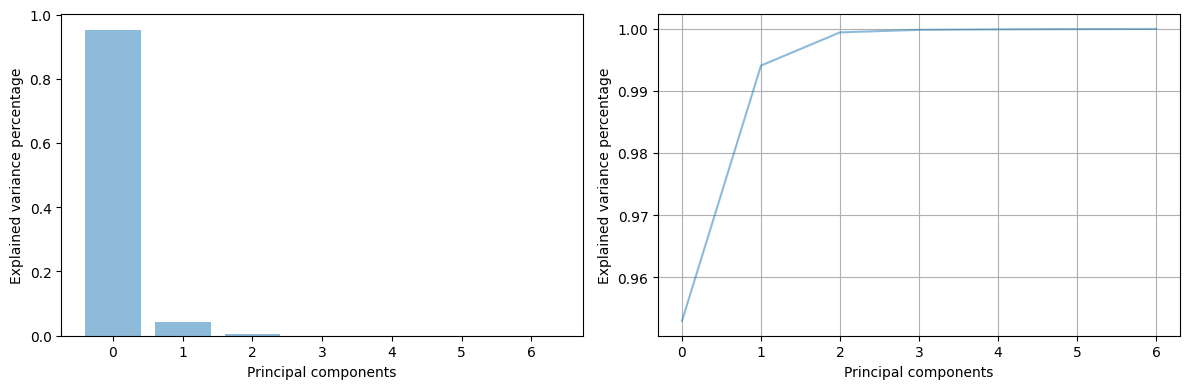
\includegraphics[width=\linewidth]{figures/pca_explained_variance}
	\caption{(left) Variance explained by each principal component. (right) Cumulative explained variance.}
	\label{fig:pca_explained_variance}
\end{figure}

The matrix made of the components values is called the \emph{loading matrix} and represents $X$ in the new coordinates.

\begin{ioutput}
          PC1     PC2     PC3     PC4     PC5     PC6     PC7
DGS1   0.5531  0.5219  0.4068 -0.5032  0.0142 -0.0498 -0.0073
DGS2   0.5484  0.2293 -0.0587  0.7846 -0.1420  0.0332  0.0785
DGS5   0.4014 -0.1873 -0.4582 -0.1051  0.6647  0.0586 -0.3706
DGS7   0.3307 -0.3223 -0.3483 -0.2636 -0.1468 -0.0413  0.7566
DGS10  0.2792 -0.3737 -0.1011 -0.1424 -0.6269 -0.3044 -0.5157
DGS20  0.1804 -0.4297  0.3907 -0.0105 -0.0624  0.7893 -0.0546
DGS30  0.1103 -0.4600  0.5802  0.1733  0.3451 -0.5249  0.1215
\end{ioutput}

Let's check the loading values for the first three components as shown in Fig.~~\ref{fig:yield_pca_components}.

\begin{itemize}
\item PC1 (green): all loads are positive, implying that the PC1 factor causes the movement of the yield curve in the same direction. Therefore, this factor is responsible for the level change. This reflects that short-term yields tend to move more than long-term yields since the loads on the short end are larger. Moreover, this figure demonstrates that most of the variance is accumulated in PC1.
\item PC2 (orange): the loading decreases from a positive value at the short end to a negative value at the long end. Furthermore, it crosses zero one time between two (2Y) and five (5Y) years bonds (this crossing point is said \emph{anchor point}). This indicates that short-term yields and long-term yields tend to move in different directions, so it describes the change in slope of the curve.
\item PC3 (blue): the loadings from short to long-term cross zero twice, which means that the very short-term and long-term yields move in the same direction while the ”belly” part of the curve has the tendency to move in the opposite direction. This factor represents the curvature of the curve in a natural way.
\end{itemize}

\begin{figure}[hbtp]
	\centering
	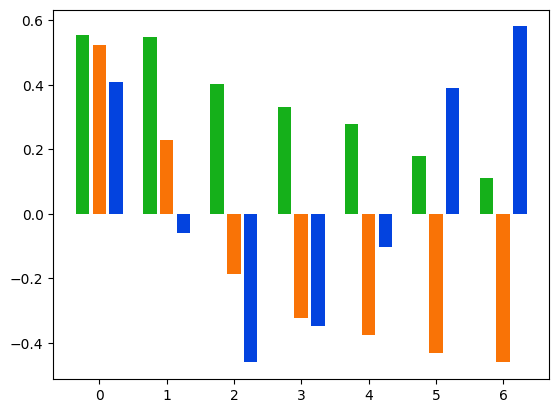
\includegraphics[width=0.45\linewidth]{figures/pca_loading_matrix}
	\caption{Components values after having performed PCA.}
	\label{fig:yield_pca_components}
\end{figure}

When the underlying factors have been found from PCA, we can finally use few principal components to approximate the original data $X$. As we observed above, almost 100\% of the variance can be explained by the first three components therefore, we will use those components to construct $\tilde{X}^{(3)}$.

Upper plots of Figures~\ref{fig:pca_dsg5},~\ref{fig:pca_dsg10} and~\ref{fig:pca_dsg30} shows the approximation of bond yield 5Y, 10Y and 30Y by all PCs in aggregate.
The corresponding residual $R^{(3)}$ are reported in the lower plots.

For 5Y rate it can be seen that even just PC1 is quite adequate to obtain a very close result with an error of the order of $10^{-3}$. In the 10Y bond approximation: PC1 has the dominant explanatory power, its residuals are about $10^{-3}$. Adding PC2 improves the reconstruction so that the residuals are roughly $10^{-4}$, and including PC3, in addition, makes no appreciable difference. This means that PC1 and PC2 are sufficient to provide an explanation of the dynamics. Our last approximation is for 30Y bonds. In comparison to the 10Y curve, PC2 is more significant in explaining the 30Y trends. Moreover, in this case, the contribution of PC3 is much more substantial.

\begin{figure}[htb]
	\centering
	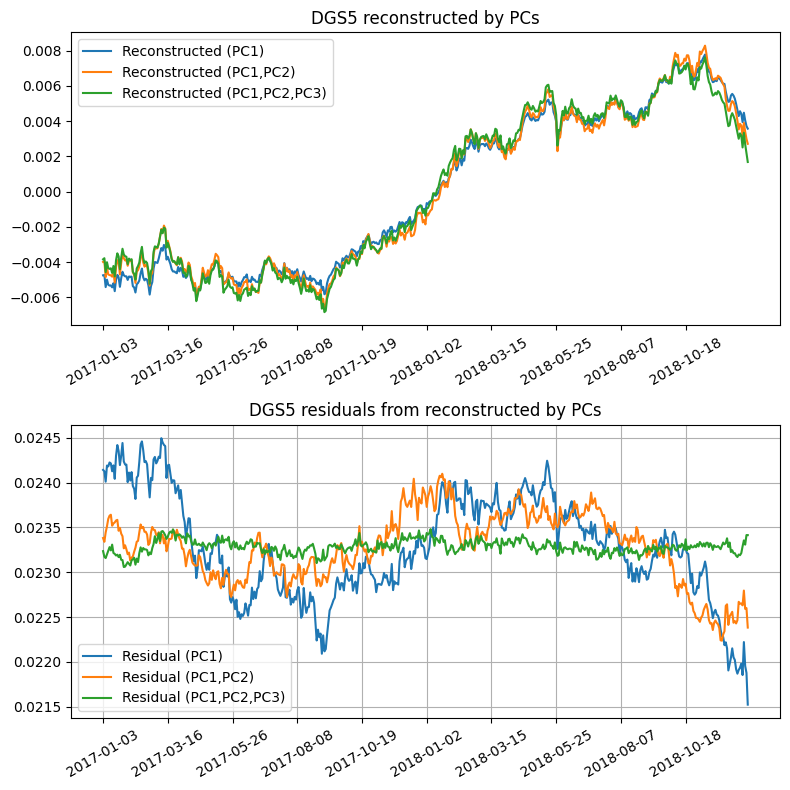
\includegraphics[width=0.6\linewidth]{figures/dgs5_reco}
	\caption{DGS5 reconstruction by PCs (top). Residuals with original data by components (down).}
	\label{fig:pca_dsg5}
\end{figure}

\begin{figure}[hp]
	\centering
	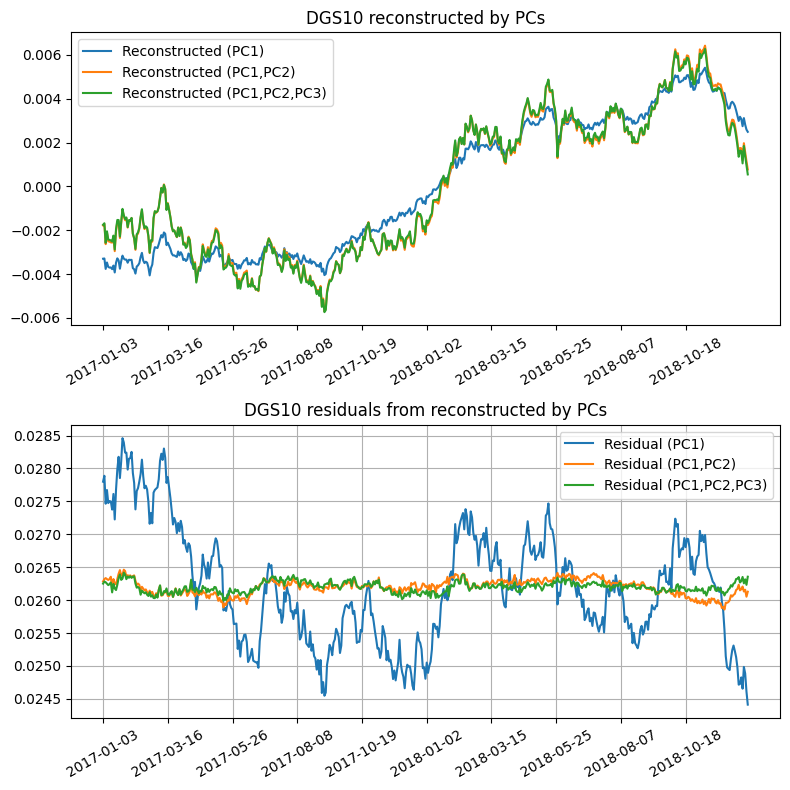
\includegraphics[width=0.65\linewidth]{figures/dgs10_reco}
	\caption{DGS10 reconstruction by PCs (top). Residuals with original data by components (down).}
	\label{fig:pca_dsg10}
\end{figure}

\begin{figure}[hp]
	\centering
	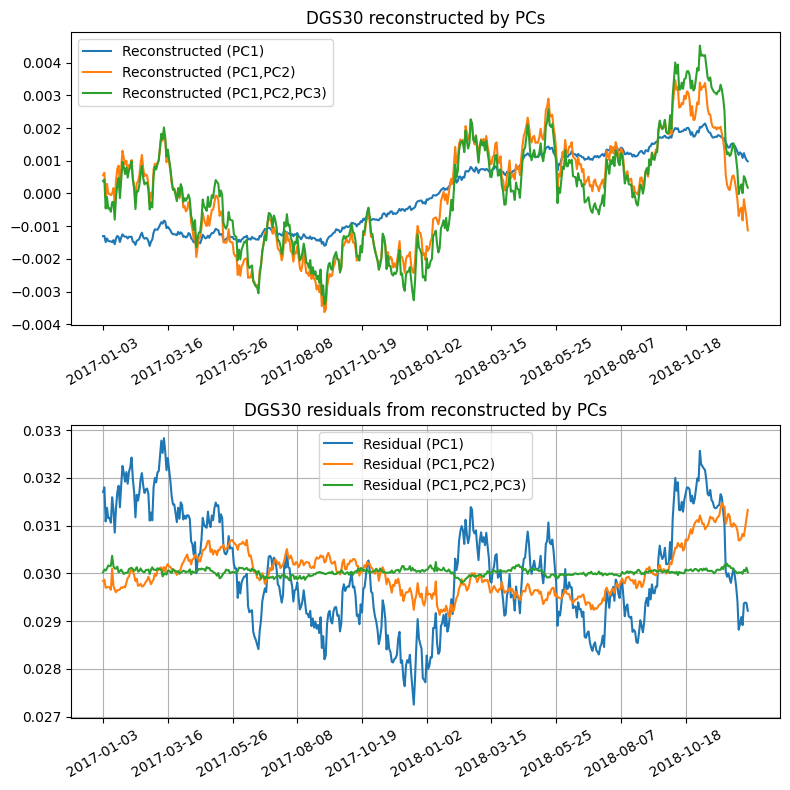
\includegraphics[width=0.65\linewidth]{figures/dgs30_reco}
	\caption{DGS30 reconstruction by PCs (top). Residuals with original data by components (down).}
	\label{fig:pca_dsg30}
\end{figure}

\newpage
\section*{Exercises}

\cprotEnv\begin{question}
The Dow-Jones Industrial Average (DJIA) was first introduced by Charles Dow in 1896 and has since become one of the main references for stock market performance on the New York Stock Exchange.

In this post, we will use it to better understand the pros and cons of simple Linear Regression models, the assumptions they rely on, and how we can use them for feature selection.

Its value is determined with a weighted average of 30 stock prices. Since the Dow components change over time, using the provided dataset (\href{"https://github.com/matteosan1/finance_course/raw/master/input_files/dji.csv}{dji.csv}) and a list of 35 assets, determine which of them are included in the calculation given a time interval. Try to interpret the results.

\textbf{Hint}: in order to cross-check your result split the dataset in two parts (before and after August 2020), then fit the model with the first part and test it with the second.
\begin{ipython}
selected = ['AAPL', 'AMGN', 'AXP', 'BA', 'CAT', 'CRM', 'CSCO', 'CVX', 'DD', 'DIS', 
            'DOW', 'GE', 'GS', 'HD', 'HON', 'IBM', 'INTC', 'JNJ', 'JPM', 'KO', 'MCD', 
            'MMM', 'MRK', 'MSFT', 'NKE', 'PFE', 'PG', 'RTX', 'TRV', 'UNH', 'V', 'VZ', 
            'WBA', 'WMT', 'XOM']
\end{ipython}
\end{question}

\cprotEnv\begin{solution}
Load the dataset and split into two dataframes DJI and the other tickers.
\begin{ipython}
import pandas as pd

closing = pd.read_csv("dji.csv", index_col='Date')
DJI = closing['DJI'].copy()
closing.drop(columns='DJI', inplace=True)
\end{ipython} 
	
\begin{figure}[htbp]
\centering
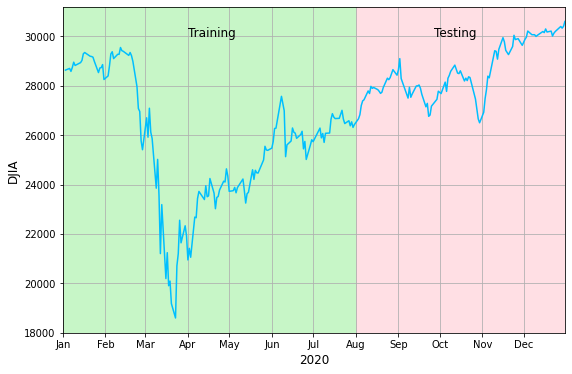
\includegraphics[width=0.7\textwidth]{figures/dji}
\caption{DJIA index daily values in 2020. The dataset has been divided into two parts for training and testing purpose.}
\label{fig:dji-returns}
\end{figure}
	
We need to fit the linear model to the available data prior to August 2020 (\emph{notice that the dataset already contains the intercept column to take care of the $\alpha$ parameter}), see Fig.~/ref{fig:dji-returns}.
\begin{ipython}
import statsmodels.api as sm

model = sm.OLS(DJI[DJI.index <='2020-07-31'], 
               closing[closing.index <='2020-07-31']).fit()
print (model.summary())
\end{ipython}
\begin{ioutput}
                          OLS Regression Results                            
==============================================================================
Dep. Variable:                    DJI   R-squared:                       1.000
Model:                            OLS   Adj. R-squared:                  1.000
Method:                 Least Squares   F-statistic:                 2.107e+06
Date:                Tue, 08 Nov 2022   Prob (F-statistic):          1.99e-297
Time:                        18:16:13   Log-Likelihood:                -364.32
No. Observations:                 143   AIC:                             800.6
Df Residuals:                     107   BIC:                             907.3
Df Model:                          35                                         
Covariance Type:            nonrobust                                         
==============================================================================
coef    std err          t      P>|t|      [0.025      0.975]
------------------------------------------------------------------------------
AAPL          28.1315      0.238    118.405      0.000      27.660      28.602
AMGN           0.0701      0.098      0.714      0.477      -0.124       0.265
AXP            6.2508      0.261     23.940      0.000       5.733       6.768
BA             7.0296      0.047    149.349      0.000       6.936       7.123
CAT            6.8530      0.160     42.953      0.000       6.537       7.169
CRM            0.0452      0.123      0.367      0.714      -0.199       0.289
CSCO           6.9258      0.564     12.274      0.000       5.807       8.044
CVX            7.6117      0.260     29.233      0.000       7.096       8.128
DD             0.4722      0.318      1.484      0.141      -0.159       1.103
DIS            6.9450      0.178     39.057      0.000       6.593       7.298
DOW            6.3940      0.387     16.541      0.000       5.628       7.160
GE             0.2437      0.216      1.130      0.261      -0.184       0.671
GS             6.9331      0.122     56.636      0.000       6.690       7.176
HD             6.6309      0.096     69.009      0.000       6.440       6.821
HON           -0.3708      0.193     -1.918      0.058      -0.754       0.012
IBM            7.3397      0.202     36.317      0.000       6.939       7.740
INTC           6.5288      0.199     32.789      0.000       6.134       6.924
JNJ            6.7114      0.240     27.962      0.000       6.236       7.187
JPM            6.7418      0.236     28.578      0.000       6.274       7.209
KO             6.9641      0.572     12.173      0.000       5.830       8.098
MCD            6.8349      0.150     45.446      0.000       6.537       7.133
MMM            6.4935      0.146     44.401      0.000       6.204       6.783
MRK            7.5556      0.318     23.792      0.000       6.926       8.185
MSFT           6.4336      0.155     41.509      0.000       6.126       6.741
NKE            6.7713      0.231     29.369      0.000       6.314       7.228
PFE            8.0045      0.466     17.163      0.000       7.080       8.929
PG             7.0308      0.294     23.894      0.000       6.447       7.614
RTX            8.4790      0.301     28.136      0.000       7.882       9.076
TRV            6.7275      0.194     34.767      0.000       6.344       7.111
UNH            6.7560      0.073     93.183      0.000       6.612       6.900
V              7.2610      0.174     41.824      0.000       6.917       7.605
VZ             6.6514      0.631     10.546      0.000       5.401       7.902
WBA            6.2044      0.331     18.750      0.000       5.548       6.860
WMT            6.7940      0.211     32.258      0.000       6.376       7.212
XOM            6.0549      0.487     12.435      0.000       5.090       7.020
intercept     -4.1082     21.263     -0.193      0.847     -46.259      38.043
==============================================================================
Omnibus:                       19.720   Durbin-Watson:                   2.012
Prob(Omnibus):                  0.000   Jarque-Bera (JB):               62.557
Skew:                          -0.398   Prob(JB):                     2.61e-14
Kurtosis:                       6.141   Cond. No.                     5.70e+04
==============================================================================
\end{ioutput}

From the $p$-values in Figure~\ref{fig:p-values} (left), we can quickly identify the stocks whose weights are not meaningfully different from zero, namely: AMGN, CRM, DD, GE, and HON. The reason is simply that they are not part of the DJIA in the considered period.
Repeating the fit with the updated model shows that all the included tickers are still contributing to the DJIA index determination, see Fig.~\ref{fig:p-values} (right).
	
\begin{ipython}
selected_columns = list(model.pvalues[model.pvalues<0.05].index)

model_small = sm.OLS(DJI[DJI.index <= '2020-07-31'], 
                     closing[selected_columns][closing.index <= '2020-07-31']).fit()
print (model_small.summary())
\end{ipython}
\begin{ioutput}
                        OLS Regression Results                                
==============================================================================
Dep. Variable:                    DJI   R-squared (uncentered):          1.000
Model:                            OLS   Adj. R-squared (uncentered):     1.000
Method:                 Least Squares   F-statistic:                 2.434e+08
Date:                Thu, 26 Jan 2023   Prob (F-statistic):               0.00
Time:                        11:59:44   Log-Likelihood:                -369.56
No. Observations:                 143   AIC:                             799.1
Df Residuals:                     113   BIC:                             888.0
Df Model:                          30                                                  
Covariance Type:            nonrobust                                                  
==============================================================================
                 coef    std err          t      P>|t|      [0.025      0.975]
------------------------------------------------------------------------------
AAPL          28.1695      0.229    123.120      0.000      27.716      28.623
AXP            6.2176      0.250     24.878      0.000       5.722       6.713
BA             7.0379      0.045    157.710      0.000       6.949       7.126
CAT            6.7754      0.133     50.871      0.000       6.511       7.039
CSCO           7.2883      0.535     13.620      0.000       6.228       8.348
CVX            7.5201      0.239     31.522      0.000       7.047       7.993
DIS            6.8027      0.163     41.760      0.000       6.480       7.125
DOW            6.6917      0.338     19.793      0.000       6.022       7.361
GS             6.9423      0.116     59.693      0.000       6.712       7.173
HD             6.6851      0.089     75.149      0.000       6.509       6.861
IBM            7.2860      0.196     37.126      0.000       6.897       7.675
INTC           6.4310      0.189     34.007      0.000       6.056       6.806
JNJ            6.7935      0.215     31.583      0.000       6.367       7.220
JPM            6.8400      0.214     31.945      0.000       6.416       7.264
KO             6.5188      0.494     13.206      0.000       5.541       7.497
MCD            6.7657      0.139     48.518      0.000       6.489       7.042
MMM            6.4385      0.121     53.174      0.000       6.199       6.678
MRK            7.5965      0.296     25.622      0.000       7.009       8.184
MSFT           6.5577      0.134     48.935      0.000       6.292       6.823
NKE            6.7307      0.208     32.385      0.000       6.319       7.142
PFE            8.0817      0.454     17.806      0.000       7.182       8.981
PG             6.9862      0.267     26.144      0.000       6.457       7.516
RTX            8.6628      0.275     31.476      0.000       8.118       9.208
TRV            6.5894      0.181     36.417      0.000       6.231       6.948
UNH            6.6966      0.066    100.982      0.000       6.565       6.828
V              7.2778      0.160     45.487      0.000       6.961       7.595
VZ             6.3851      0.526     12.134      0.000       5.343       7.428
WBA            6.2725      0.304     20.631      0.000       5.670       6.875
WMT            6.9055      0.198     34.832      0.000       6.513       7.298
XOM            6.5498      0.443     14.782      0.000       5.672       7.428
==============================================================================
Omnibus:                       27.413   Durbin-Watson:                   1.905
Prob(Omnibus):                  0.000   Jarque-Bera (JB):               91.998
Skew:                          -0.630   Prob(JB):                     1.05e-20
Kurtosis:                       6.722   Cond. No.                     1.70e+03
==============================================================================
\end{ioutput}
\begin{figure}[htbp]
\centering
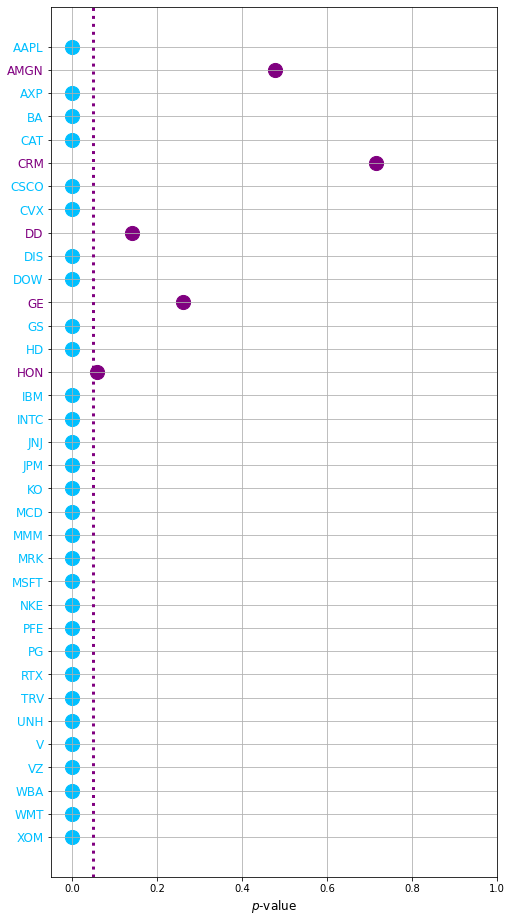
\includegraphics[width=0.4\textwidth]{figures/p-values}
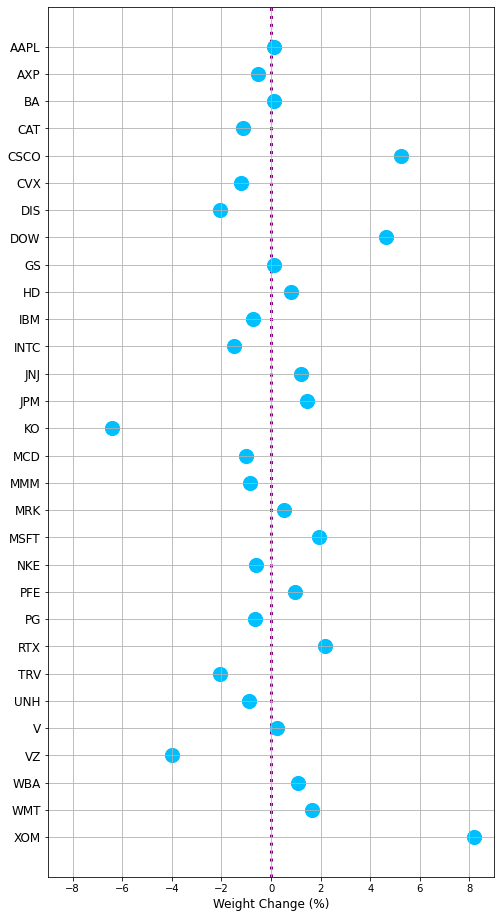
\includegraphics[width=0.4\textwidth]{figures/delta_weights}
\caption{$p$-values resulting from the linear model fit to DJIA returns (left). Parameter percentage difference according to the two models described in the text (right).}
\label{fig:p-values}
\end{figure}
	
Now that we have a good model it is possible to check how it behaves on the test sample (i.e. from August to December 2020). The result is shown in Figure~\ref{fig:prediction}. The residuals plot, the difference between predicted and actual values of the DJIA, shows that there is a clear degradation of the performance after September, see Fig.~\ref{fig:residuals}.

\begin{ipython}
residuals = DJI-model_small.predict(closing[selected_columns])
\end{ipython}
	
\begin{figure}[htbp]
\centering
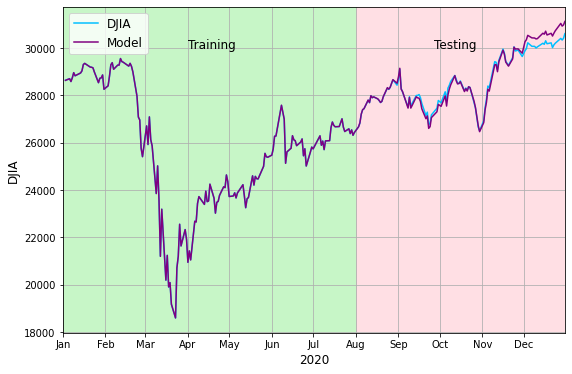
\includegraphics[width=0.7\textwidth]{figures/prediction}
\caption{Model prediction to DJIA index performance comparison.}
\label{fig:prediction}
\end{figure}

As we can see, our model works extremely well for the first few weeks of the testing period and then it completely falls apart. The reason for this puzzling behavior is surprisingly simple: the fundamental assumption underlying our model was no longer valid. The \textbf{composition of the DJIA changed on Aug 31st, 2020} with Pfizer, Raytheon, and Exxon Mobile being dropped and replaced by Amgen, Honeywell, and Salesforce.

\begin{figure}[htbp]
\centering
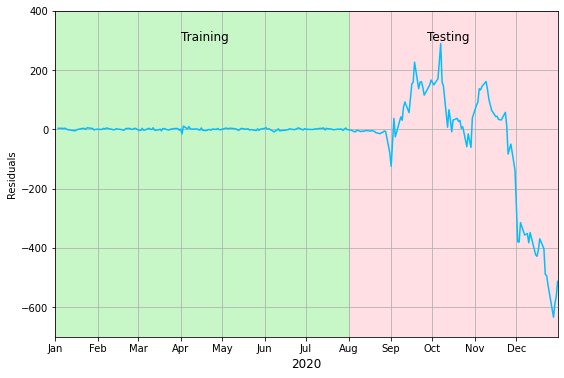
\includegraphics[width=0.7\textwidth]{figures/residuals}
\caption{Residuals of the linear model.}
\label{fig:residuals}
\end{figure}
\end{solution}

\begin{question}
Stock A has a $\beta$ of 1.2 and Stock B has a $\beta$ of 0.6. Which of the following statements is true? 
\begin{enumerate}[label=\emph{\alph*})]
\tightlist
\item Stock A has more unsystematic risk than Stock B;
\item Stock B has more systematic risk than Stock A; 
\item if the risk-free rate and the market risk premium are both positive, Stock A has a higher expected return than Stock B according to the CAPM;
\item both \emph{a} and \emph{b} are true;
\item both \emph{b} and \emph{c} are true
\end{enumerate}
\end{question}

\begin{solution}
The correct answer is \emph{c} indeed according to CAPM formula
\[r_i = r_f + \beta_i (r_M - r_f)\]
if both $r_f$ and $(r_M - r_f)$ are positive then $r_A > r_B$.
\end{solution}	

\begin{question}
Consider a stock with a $\beta$ of 1.5. Which of the following statements is true?

\begin{enumerate}[label=\emph{\alph*}]
\tightlist
\item when the market goes down by 1.5\%, on average, the stock goes down by 1\%;
\item when the market goes up by 1.5\%, on average, the stock goes up by 1\%;
\item when the market goes up by 1\%, on average, the stock goes down by 1.5\%;
\item when the market goes down by 1\%, on average, the stock goes down by 1.5\%. 
\item both \emph{a} and \emph{b}.	
\end{enumerate}
\end{question}

\begin{solution}
The correct answer is \emph{d} since $\beta$ measures the slope of the regression line of the expected return of the stock vs the expected return of the market. So by definition it represents the variation of the stock expected return given the a unit variation of the expected return of the market.
\end{solution}	

\begin{question}
Suppose that the risk-free rate is 3\% and the market risk premium is 8\%. According to the CAPM, what is the required rate of return on a stock with a $\beta$ of 2 ?
\end{question}

\begin{solution}
Careful! The market risk premium is 8\%. This means that $r_M - r_f  = 8\%$. Plug this into the CAPM equation to get

\begin{equation*}
r = r_f + \beta(r_M - r_f) = 3\% + 2\cdot(8\%) =19\%
\end{equation*}
\end{solution}

\begin{question}
You analyze the prospects of several companies and come to the following conclusions about the required return on each:

\begin{center}
\begin{tabular}{lc}
\textbf{Stock Required} & \textbf{Return} \\
Starbucks &18\% \\
Sears &8\% \\
Microsoft &16\% \\
Limited Brands &12\% \\
\end{tabular}
\end{center}

You decide to invest \$4000 in Starbucks, \$6000 in Sears, \$12000 in Microsoft, and \$3000 in Limited Brands. What is the required return on your portfolio?
\end{question}

\cprotEnv \begin{solution}
\begin{ipython}
P = 4000 + 6000 + 12000 + 3000
rp =(4000/P)*0.18 + (6000/P)*0.08 + (12000/P)*0.16 +(3000/P)*0.12
print (f"Portfolio Return: {rp*100:.2f}%")
\end{ipython}
\begin{ioutput}
Portfolio Return: 13.92%
\end{ioutput}
\end{solution}	

\begin{question}
You have a portfolio that consists of 35\% Microsoft stock, 35\% Amazon stock, and 30\% GE stock. Microsoft has a $\beta$ of 1, Amazon has a $\beta$ of 3.0, and GE has a $\beta$ of 0.5. Treasury bills (the risk-free asset) currently offer a return of 4\%, and the expected return on the market is 11.5\%. What return should you expect on your portfolio according to the CAPM ? 
\end{question}

\cprotEnv \begin{solution}
You can work this problem two different ways.

\textbf{Method 1}: calculate the $\beta$ of your portfolio and plug this $\beta$ into the CAPM formula to get the required return of your portfolio.

\begin{ipython}
rm = 0.115
rf = 0.04
beta_p = 0.35 * 1 + 0.35 * 3 + 0.3 * 0.5
rp = rf + beta_p*(rm - rf)

print (f"Portfolio beta: {beta_p:.2f}")
print (f"Portfolio return: {rp*100:.3f}%")
\end{ipython}
\begin{ioutput}
Portfolio beta: 1.55
Portfolio return: 15.625%
\end{ioutput}

\textbf{Method 2}: using the CAPM, calculate the required return on each individual stock. Then,calculate the weighted average of those required returns to get the required return of your portfolio.

\begin{ipython}
Er_msft = rf + 1*(rm-rf)
Er_amzn = rf + 3*(rm-rf)
Er_ge = rf + 0.5*(rm-rf)
rp2 = Er_msft * 0.35 + Er_amzn *0.35 + Er_ge * 0.3

print (f"Er (MSFT): {Er_msft*100:.2f}%")
print (f"Er (AMZN): {Er_amzn*100:.2f}%")
print (f"Er (GE): {Er_ge*100:.2f}%")
print (f"Portfolio return: {rp2*100:.3f}%")
\end{ipython}
\begin{ioutput}
Er (MSFT): 11.50%
Er (AMZN): 26.50%
Er (GE): 7.75%
Portfolio return: 15.625%
\end{ioutput}
Notice that this is the same answer we got using method 1. When calculating the required return of a portfolio, it does not matter which way you do it. But method 1 is a little less work.
\end{solution}


\chapter{Modeling Risk Correlation}

In credit derivative valuation and credit risk management, one of the most important issues is the estimate of default probabilities and their correlations. Two are the possible ways to address this task: using historical default data or mathematical models.

Historical default data has played an important role in the estimate of default probabilities in the past. However, because credit events are rare, there is very limited data available. Moreover, historical data only reflects the past default patterns and it may not be a proper indicator of the future. This makes such technique difficult and inexact. To use this same data to estimate default correlations is even more difficult and inexact.

The market trend now is towards the use of mathematical models that don't rely on historical default data. In Chapter~\ref{sec:credit-default-swaps} we have seen how it is possible to derive default probabilities from market data, here we will see how copulas can be used to model their correlations to evaluate credit derivatives. 

\section{Correlation}
\label{sec:default_correlation}
Correlation is a quantitative measure that evaluates how consistently two variables move together relative to their respective sample means. 

It assesses alignment in deviations rather than raw magnitudes: \emph{positive alignment} both variables lie above (or below) their respective averages simultaneously, \emph{negative alignment} one variable lies above its average while the other lies below.

Mathematically, the standard measure for linear co-movement is the Pearson correlation coefficient ($\rho$):

$$\rho = \frac{\text{Cov}(X,Y)}{\sigma_X \sigma_Y}$$
Covariance ($\text{Cov}(X,Y)$) captures the directional co-variability of the two variables relative to their means. Dividing by the product of the standard deviations scales the result to a standardized range between $-1$ and $+1$:
\begin{itemize}
	\item $+1.0$: perfect positive linear relationship;
	\item $0.0$: no linear relationship;
	\item $-1.0$: perfect negative linear relationship.
\end{itemize}	

In the case of $N>2$ assets, $\rho$ is a symmetric matrix (sometimes also indicated by $\Sigma$).

\begin{equation*}
	\Sigma = \begin{bmatrix}
		\sigma^2 (X_0) & \cov(X_0, X_1) & \cov(X_0, X_2)\\
		\cov(X_1, X_0) & \sigma^2 (X_1) & \cov(X_1, X_2)\\
		\cov(X_2, X_0) & \cov(X_2, X_1) & \sigma^2 (X_2)\\
	\end{bmatrix}
\end{equation*}
Diagonal terms report the variance of each random variable, while the non-diagonal terms represent the correlation between each pair of variables. The matrix is symmetric since the correlation between $X_i$ and $X_j$ is the same as between $X_j$ and $X_i$.

Correlation is not an explanatory tool, but an initial diagnostic signal. It identifies statistically significant co-movements within datasets, establishing baseline patterns that warrant further domain specific investigation and formal causal inference models.
High correlation between two variables is frequently driven by an unobserved third variable (e.g., ambient temperature independently increasing both ice cream sales and swimming activities). Pearson correlation specifically measures the degree to which a linear function describes the relationship. It fails to detect strong non-linear dependencies (e.g., $y = x^2$ yields $\rho \approx 0$ over symmetric domains despite being deterministically related).

The challenge to do a good Monte Carlo simulation to model asset defaults relies on the ability to generate realistic scenarios. That is, being able to be loyal to the average default probability of the pool and to the assets’ default correlation $\rho$. 

\begin{figure}[htb]
	\centering
	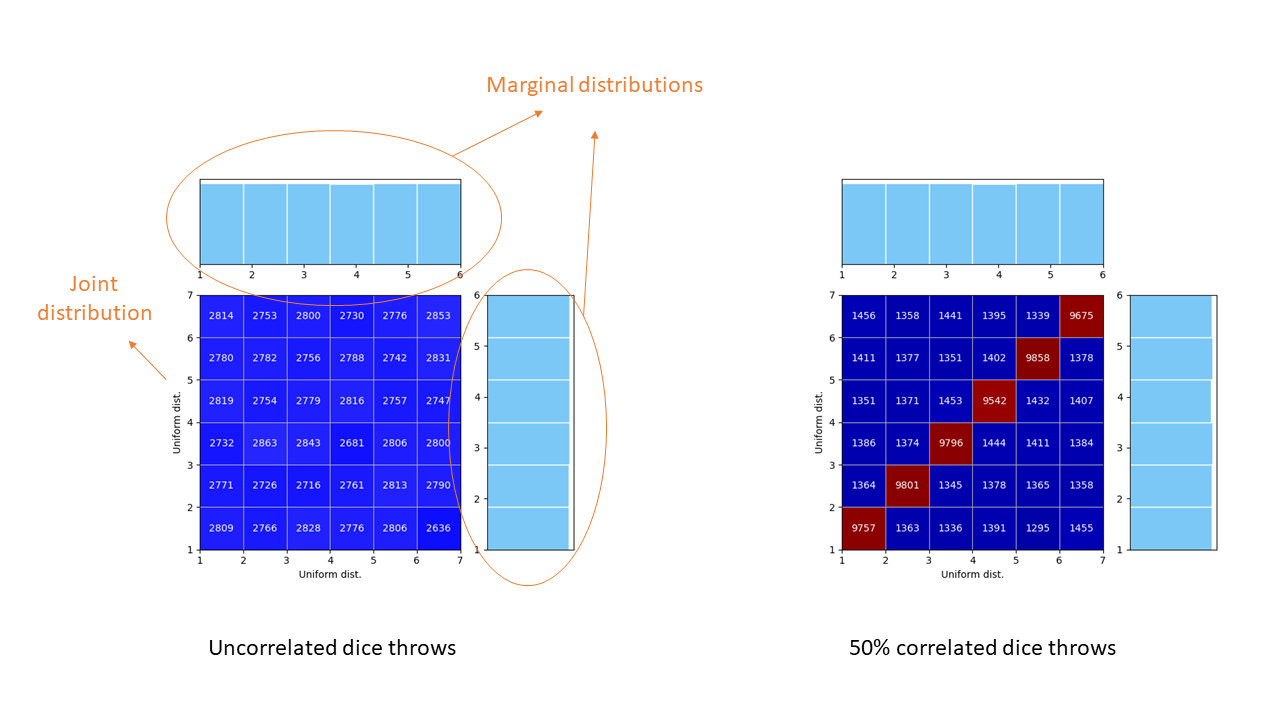
\includegraphics[width=0.9\textwidth]{figures/marginal_joint_correlation}
	\caption{Notice that correlation doesn't affect marginal distribution !}
	\label{fig:marginal_joint}
\end{figure}

\section{Distribution Transformation}
\label{sec:distribution-transformation}

Distribution transformation is a very useful tool which will be extensively used with the copula. This technique allows to transform every random variable distribution into uniform and vice versa and is called \emph{inverse transform} (or \emph{probability integral transform}).
It involves computing the cumulative distribution function $F_{X}$ (or its inverse) which maps a number to a probability between 0 and 1. 

\begin{attention}
\subsubsection{Demonstration}
Let's start with a random variable $X$ and let $F_X$ be its cumulative distribution function ($F(x) = P(X \leq x)$).
We would like to find a transformation $T:[0,1]\rightarrow\mathbb{R}$ such that $T(U)=X$, where $U$ is the uniform distribution in $[0,1]$. 
\begin{equation*}
F_X(x)= P(X\leq x)=P(T(U)\leq x)= P(U\leq T^{-1}(x))=T^{-1}(x),{\text{ for }}x\in \mathbb {R}
\end{equation*}
where the last step used that $P(U\leq y)=y$ when $U$ is uniform on $(0,1)$.

So we got $F_{X}$ to be the inverse function of $T$, or, equivalently $T(u)=F_{X}^{-1}(u)$, $u\in [0,1]$, hence $T$ is the \textbf{quantile function}.
\end{attention}

To transform a generic random variable to uniform (and vice versa) we can use
\begin{equation}
x = F_{X}^{-1}(u)\quad\mathrm{and}\quad u = F_X(x)	
\end{equation} 
\noindent Figure~\ref{fig:inverse_transform} shows graphically how the inverse transform works.

\begin{figure}[htb]
\centering
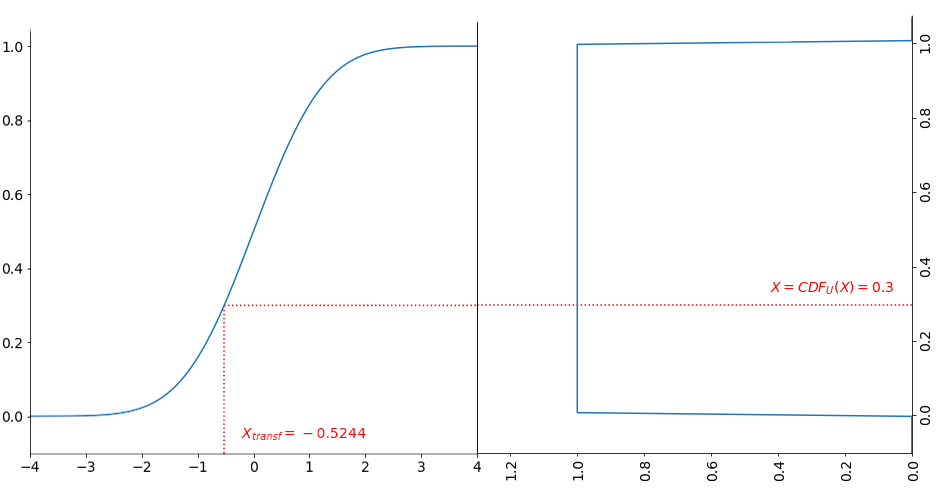
\includegraphics[width=0.9\textwidth]{figures/inverse_transform}
\caption{Inverse transform example. Going from right to left a sample $x$ in $[0,1]$ interval is chosen, this corresponds also to CDF$_{\text{U}}(x)$. This value is selected on the CDF of the other distribution $f$ and it is finally transformed into a sample from $f$ using the quantile function.}
\label{fig:inverse_transform}
\end{figure}

Imagine we want to transform a uniform distribution into Gaussian. The transformation takes uniform samples $u$ between 0 and 1, interpreted as a probabilities, and then returns $F_{\text{normal}}^{-1}(u)$. The following code shows how this can be done in \texttt{python}. 

\pythoncode{code/modelling_risk_1.py}

We start by generating a sample from the uniform distribution using \texttt{scipy.stats.uniform}, line 3. 
In the left plot of Fig.~\ref{fig:a_to_b_to_a} the resulting distribution is shown.
Next we want to transform the sample so that it becomes normally distributed. The transformation to use is the quantile function of the normal distribution, or $(\tt{ppf(x))}$. Remember that all the methods of \texttt{scipy.stats} applied to \texttt{numpy.array} works on each item of the array without the need to make explicit for-loops.
In the mid plot of Fig.~\ref{fig:a_to_b_to_a} the Gaussian obtained with the code below is shown

\begin{figure}[htbp]
	\centering
	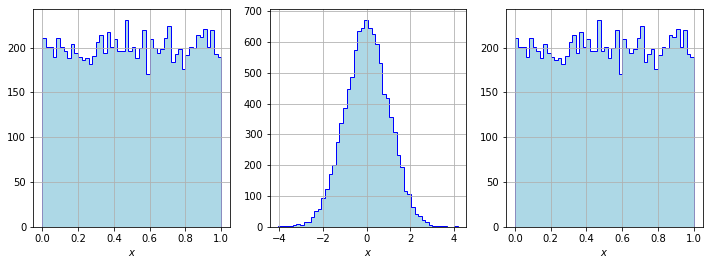
\includegraphics[width=0.8\textwidth]{figures/a_to_b_to_a}
	\caption{Example of transformation, it starts with a uniform distribution, goes into a Gaussian and back to the initial uniform.}
	\label{fig:a_to_b_to_a}
\end{figure}

If we plot the two distribution together we can get a sense of what is going on using the inverse CDF transformation. Indeed it stretches the outer regions of the uniform to yield a normal distribution. This is shown in Fig.~\ref{fig:uniform_to_gauss}. 
    
\begin{figure}[htbp]
\centering
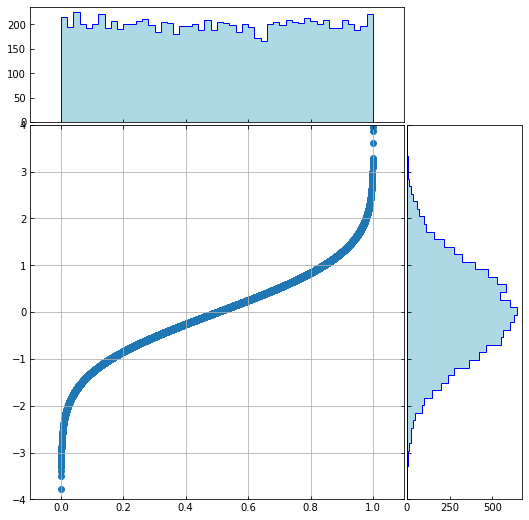
\includegraphics[width=0.6\textwidth]{figures/uniform_to_gauss}
\caption{2D plot showing the transformation that maps our initial uniform distribution to the resulting Gaussian.}
\label{fig:uniform_to_gauss}
\end{figure}
    
Clearly to do the opposite transformation, that is from an arbitrary distribution to uniform, we can just apply the inverse of the inverse CDF, that is the CDF itself, line 5.
In such a way we can go from distribution A to B passing through the uniform rather quickly as shown in three plots of Fig.~\ref{fig:a_to_b_to_a}.

Notice that this technique can be used for any arbitrary (univariate) probability distribution so you can test it with different samples. 

\section{Copula}
\label{copula}

A \emph{copula} $\mathcal{C}(F_1, F_2, \ldots, F_n, \rho)$ allows the joining of multiple univariate distributions to a single multivariate distribution. Copulas are used to describe the dependencies between random variables and have been widely used in quantitative finance to model risk. 

Its exact definition from probability theory is the following: a multivariate, i.e. multidimensional, cumulative distribution function whose \emph{marginal} probability distributions, i.e. the probability distribution of each dimension, are uniform ($F_i = U_i =\mathrm{uniform}(0,1)$), $\rho$ represents the correlation between each variable.

A key part of copulas is the \emph{Sklar’s theorem}. It states that given a joint distribution $F(x_1, x_2, \dots, x_d)$ for $d$ variables with continouos marginals $F_1(x_1), \dots, F_d(x_d)$, there exists a unique copula $\mathcal{C}$ such that:

$$F(x_1, x_2, \dots, x_d) = \mathcal{C}\Big(F_1(x_1), F_2(x_2), \dots, F_d(x_d)\Big)$$
If $u_i = F_i(x_i) \sim U(0,1)$, the copula function maps the marginal uniform probability distributions into the joint distribution.

This property makes them very popular since allow to easily model the distribution of correlated random variables by representing marginals and correlation separately: essentially allow to split a complicated problem into simpler components.

\begin{attention}
Mathematically, the theorem can be stated as follows: suppose we have only two random variables, $X$ and $Y$. If $F(x,y)$ is a joint distribution function with continuous marginals $f_x(x)=u$ and $f_y(y)=v$, then the joint distribution $F(x,y)$ can be written in terms of a unique function $\mathcal{C}(u,v)$:
\begin{equation}
F(x,y)=\mathcal{C}(u,v)
\end{equation}
\noindent
where $\mathcal{C}(u,v)$ is the copula of $F(x,y)$.
The copula function describes how the multivariate function $F(x,y)$ is derived from or coupled with the marginal distribution functions $f_x(x)$ and $f_y(y)$.
\end{attention}

There are a large number of copulas each characterized by a particular correlation structure. The most common ones are the \emph{Gaussian} and \emph{t-student} copulas. The former relies on a multivariate-normal correlation structure $\Phi_\Sigma$, but it couples marginals which can follow arbitrary distributions.
Mathematicaly it can be expressed as

$$\mathcal{C}_R^{\text{Gauss}}(u_1, \dots, u_d) = \Phi_\Sigma \Big( \Phi^{-1}(u_1), \dots, \Phi^{-1}(u_d) \Big)$$
where: $\Phi^{-1}$ is the inverse of the normal CDF (quantile function), and $\Phi_\Sigma$ is the multivariate normal CDF with correlation matrix $\Sigma$.

Despite the probably obscure and daunting definition given above the concept of copula is quite simple so it will be clarified with a practical example.

\section{Working with Correlated Distributions}
\label{sec:generate-correlated-distributions}

\subsection{Correlated Asset Returns}
\label{sec:correlated_stock_returns}

In this example we are going to consider the closing prices of two assets like BMW and Siemens in the period between 2010 and 2022 (the series can be found in \href{https://github.com/matteosan1/finance_course/raw/master/input_files/bmw_siemens.csv}{bmw\_siemens.csv}).

Since the two companies belongs to the same sector and to the same market it is plausible to assume that their returns are correlated, and in particular we would like to estimate the probability that both of them are negative.

From the historical series of the two assets we can determine the distributions of the individual returns irrespective of the other one, i.e. the marginals, but we don't know how we could model the correlated probability distribution, \emph{joint distribution}, with which we should work to answer our question. 

Here is where copula comes in hand, since it bridges the marginal distributions (which by definition have no correlation) into a joint probability distribution. 

In order to simulate $N$ return vectors with gaussian correlation:
\begin{enumerate}
\item Compute the correlation matrix $\Sigma$ from historical series.
\item Generate a sample from $Z \sim \mathcal{N}_d(0, \Sigma)$.
\item Compute $U_i = \Phi(Z_i)$ for each dimension $i$, so $U$ (the copula) has uniform marginals $U(0,1)$ and the wanted correlation structure.
\item Apply inverse transform transformation to each dimension to get the proper marginals.
\end{enumerate}

\begin{finmarkets}
	It may be useful to create a \texttt{python} object to handle copulas. In \texttt{finmarkets} this class is \texttt{Copula} and has a method \texttt{sample} which generates a sample from the specified type of copula with the proper correlation.
\end{finmarkets}

\pythoncodenon{code/modelling_risk_copula.py}

\begin{ipythonnon}
import pandas as pd

df = pd.read_csv("bmw_siemens.csv", index_col='Date').dropna()
corr = df.corr(method="spearman")
print (corr)
\end{ipythonnon}
\begin{ioutput}
          BMW.DE    SIE.DE
BMW.DE  1.000000  0.609494
SIE.DE  0.609494  1.000000
\end{ioutput}
Indeed the returns are correlated by about 60\% as shown in Figure~\ref{fig:bmw_sie_returns}.
\begin{attention}
You may have noticed that we are using the \textit{Sperarman's correlation} here.
A standard historical covariance matrix measures linear relationships (straight lines), assuming data moves together in a predictable, proportional way. However, real financial data is often messy, non-linear, and full of extreme shocks. To bridge this data into a copula, we use Spearman's method because it calculates correlation based on the \textbf{ranks} (the relative order) of the data rather than raw numbers. "Based on rank" means replacing the actual, raw numerical values in your dataset with their ordered positions (from smallest to largest) instead of using the numbers themselves. Instead of asking "How much did the value change?", a rank-based method asks: "Where does this value stand in line compared to the others?" This strips out distortions from outliers and captures non-linear dependencies, giving you a clean, reliable correlation matrix that fits a copula's requirement for uniform, rank-based behavior.
\end{attention}

\begin{figure}[htbp]
\centering
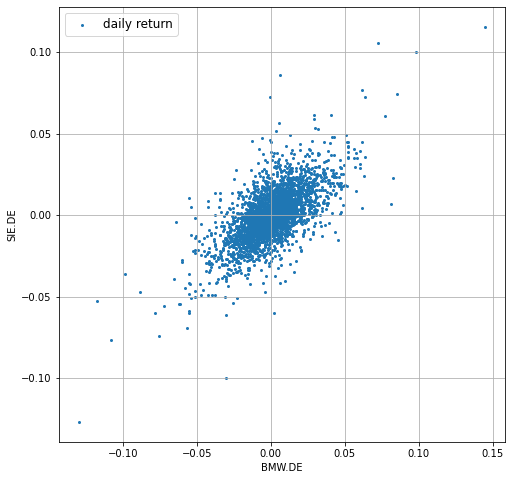
\includegraphics[width=0.6\textwidth]{figures/bmw_sie_daily_returns}
\caption{Distribution of the daily returns of BMW and Siemens stock price from 2010 to 2022.}
\label{fig:bmw_sie_returns}
\end{figure}

By fitting the return histograms, e.g. using t-student~\cite{bib:t_student} functions, we can determine the parametric form of the marginal distributions. The resulting fits are shown in Fig.~\ref{fig:bmw_sie_fit}.

\begin{ipythonnon}
bmw_fit_params = t.fit(df['BMW.DE'], fdf=5)
sie_fit_params = t.fit(df['SIE.DE'], fdf=5)

f_bmw = t(*bmw_fit_params)
f_sie = t(df=sie_fit_params[0], loc=sie_fit_params[1], 
          scale=sie_fit_params[2])	
\end{ipythonnon}

\begin{figure}[htbp]
\centering
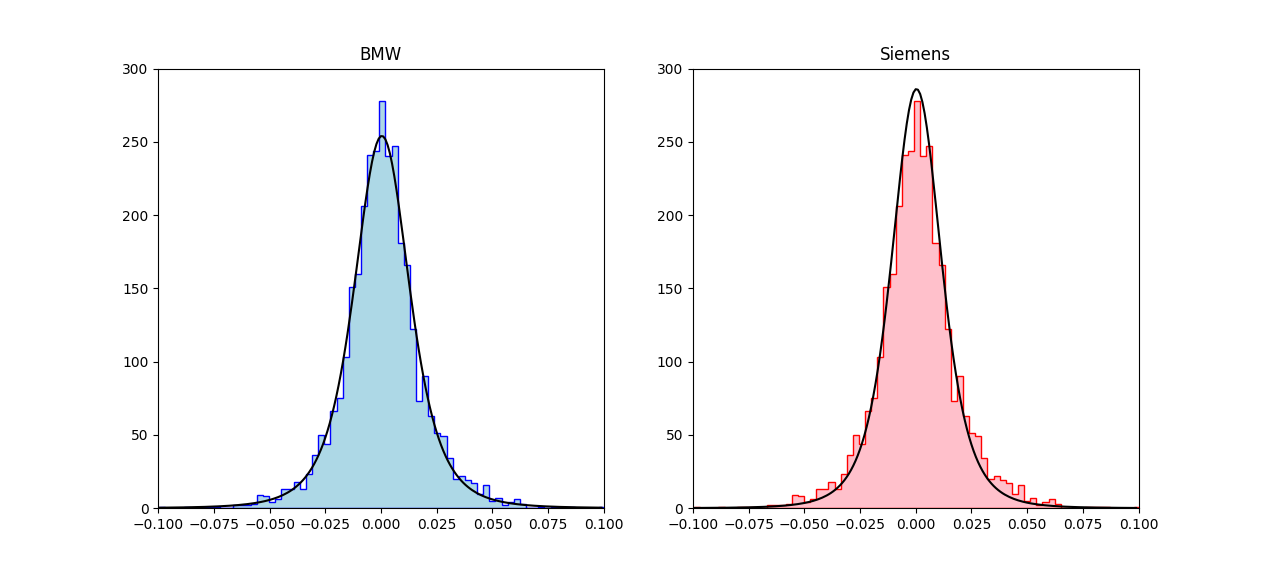
\includegraphics[width=0.75\textwidth]{figures/bmw_siemens_fit}
\caption{Fit of the daily return distributions for BMW (left) and Siemens (right). The assumed functional form is a t-student.}
\label{fig:bmw_sie_fit}
\end{figure}

To model the joint probability distribution we first have to simulate a sample from a multivariate distribution with the specific correlation structure. Right now we assume a Gaussian correlation, this is not mandatory though, later on we will see how to use other distributions.
\begin{ipythonnon}
from copulas import Copula

gauss_copula = Copula(n=2, typ="gauss", params={"mean":df.mean(), "corr": corr})
	
np.random.seed(1)
N = 1_000_000
gauss_copula.rvs(size=N)
x = gauss_copula.samples[:, 0]
y = gauss_copula.samples[:, 1]
\end{ipythonnon}

We then transform the sample so that the marginals are uniform with the technique outlined above (obtaining the copula function and the result is shown in Fig.~\ref{fig:copula}. Plots like this are how copulas are usually visualized. Since we have used a multivariate standard normal to model the correlation this is an example of \textbf{Gaussian Copula}.

\begin{figure}[htbp]
	\centering
	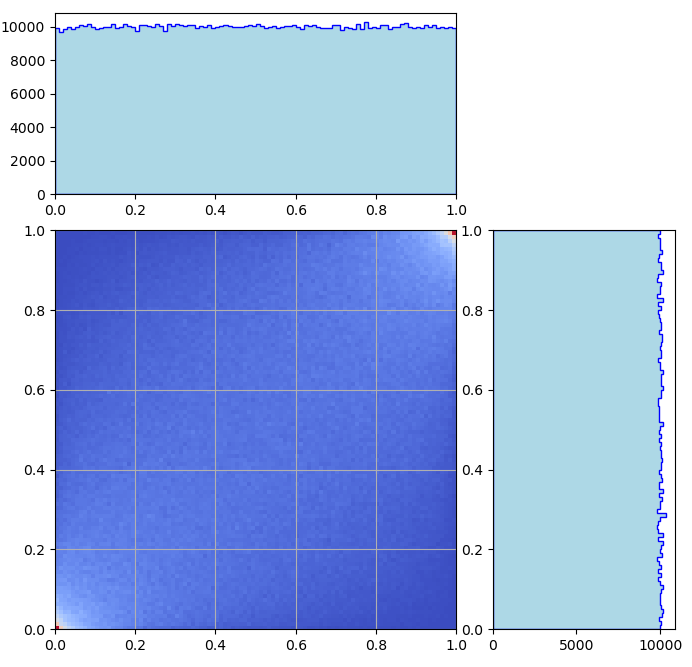
\includegraphics[width=0.45\textwidth]{figures/copula_2d}
	\quad
	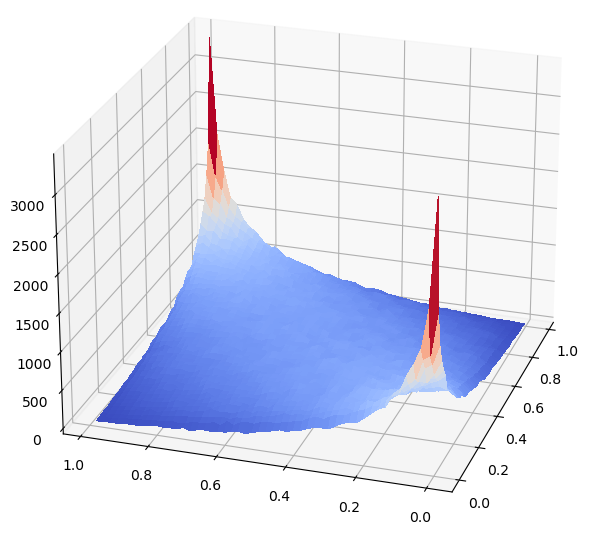
\includegraphics[width=0.5\textwidth]{figures/copula_3d}
	\caption{Graphical representations of the copula, 2D on the left, 3D on the right.}
	\label{fig:copula}
\end{figure}

At this point we can just transform the uniform marginals to the appropriate distributions (t-students in our case) to have the desired correlated distributions. 

\begin{ipythonnon}
correlated_samples = gauss_copula.rvs_marginals(distributions=[bmw_f, sie_f])
\end{ipythonnon}

Now we can reliably check the probability to have both stocks going down at the same time.
\begin{ipythonnon}
n = np.sum(np.all(correlated_samples < 0, axis=1))
print (f"Probability w/ correlation: {n/N}")
\end{ipythonnon}
\begin{ioutput}
Probability w/ correlation: 0.345859
\end{ioutput}

As a comparison let's compute the same probability this time ignoring the correlation between the returns. To do so just sample from the two marginals and count how many times they both are negative.
\begin{ipythonnon}
bmw_uncorr = bmw_f.rvs(size=N)
sie_uncorr = sie_f.rvs(size=N)

n = np.sum((bmw_uncorr < 0) & (sie_uncorr < 0))
print (f"Probability w/o correlation: {n/N}")
\end{ipythonnon}
\begin{ioutput}
Probability w/o correlation: 0.23746
\end{ioutput}

The comparison between the two multivariate distributions in Figure~\ref{fig:bmw_sie_with_corr} clearly shows the different populations in the area of interest (shaded in yellow).

\begin{figure}[htbp]
\centering
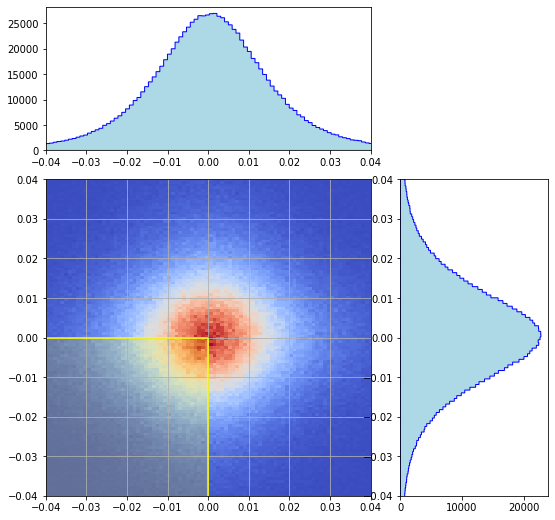
\includegraphics[width=0.45\textwidth]{figures/bmw_sie_uncorrelated}
\quad
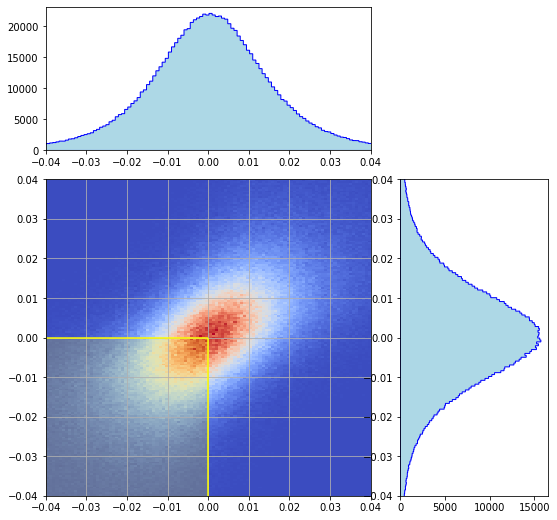
\includegraphics[width=0.45\textwidth]{figures/bmw_sie_correlated}
\caption{Marginalized t-student distributions with their joint when they are (right) and are not (left) correlated.}
\label{fig:bmw_sie_with_corr}
\end{figure}
    
Using the uniform distribution as a common base for our transformations we can easily introduce correlations and flexibly construct complex probability distributions. Everything discussed in this Section could be easily generalized to higher dimensions.

\subsubsection{Remarks on Gaussian Copula}
\begin{quote}
\textit{Extreme, synchronized rises and falls in financial markets occur infrequently but they do occur. The problem with Gaussian models is that they did not assign a high enough likelihood of occurrence to the scenario in which many things go wrong (or right) at the same time the “perfect storm” scenario.}
\end{quote}

In other words Gaussian copula is nice and easy to construct but tends to underestimate events on the tails. Indeed it is often used the t-student copula which has fatter tails but preserves the same (bell shaped, non-skewed) characteristics of the Gaussian.

This result tells us that, not only the Normal hypothesis of the return distribution is not correct, but also the Gaussian copula is not capable of correctly account for extreme events which are rare but not so much as predicted by the model.

The t-student copula instead allows a range of dependence structures depending on the $\nu$ parameter (the number of degrees of freedom of the function). It is a symmetrical copula and has larger tails than the Gaussian. 

\begin{figure}[htbp]
	\centering
	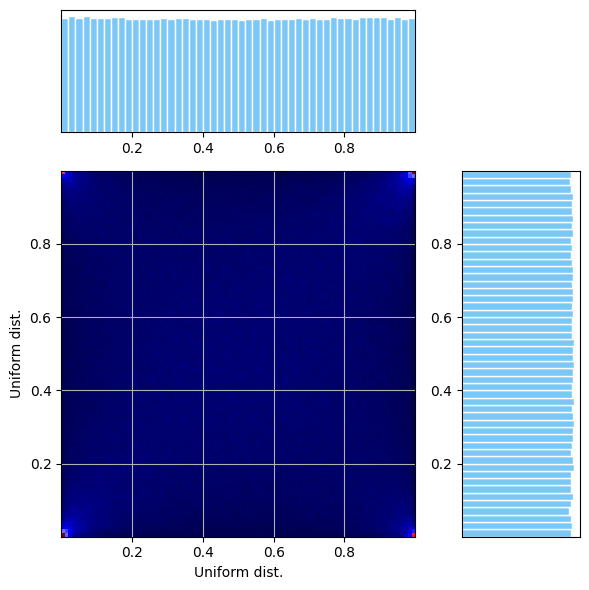
\includegraphics[width=0.45\textwidth]{figures/t-copula_2d}
	\quad
	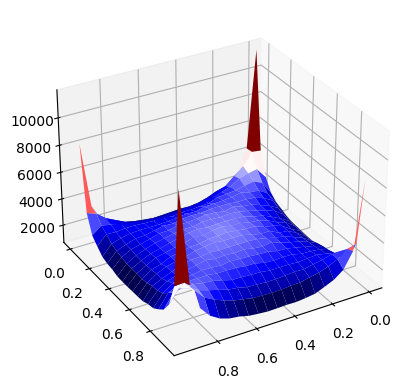
\includegraphics[width=0.5\textwidth]{figures/t-copula_3d}
	\caption{Graphical representations of the t-copula, 2D on the left, 3D on the right.}
	\label{fig:t-copula}
\end{figure}


To make this statement a little bit more quantitative we can compare the number of simultaneous extreme downturn of BMW and Siemens from the historical data to simulated events with Gaussian and t-student copulas. In this simple check we are considering an extreme event when it is $5\sigma$ away the mean.

Clearly before to proceed we need to update the \texttt{Copula} class to generate this new type of copula.

\begin{ipythonnon}
class Copula:
  def __init__(self, n: int, typ: str, params: dict):
    self.n = n
    self.type = typ.lower()
    self.mean = np.zeros(n)
    self.corr = params.get('corr')        
    self.dof = params.get('dof', 4)

    self._normalize_cov()

    if self.type == "gauss":
       self.mv = multivariate_normal(mean=self.mean, cov=self.corr)
    elif self.type == "t":
       self.mv = multivariate_t(loc=self.mean, shape=self.corr, df=self.dof)
    else:
       raise ValueError(f"Copula type {type} unknown.")
    self.x = None
    self.samples = None
  ...
  def rvs(self, size: int, seed: int=1):        
    np.random.seed(seed)
    self.x = self.mv.rvs(size=size)
    if self.type == "gauss":
      self.samples = norm.cdf(self.x)
    elif self.type == "t":
      self.samples = t(df=self.dof, loc=0, scale=1.0).cdf(self.x)
    else:
      raise ValueError(f"Copula type {type} unknown. "
                        "Available types: gauss, t")
  ...
\end{ipythonnon}

%\begin{attention}
%A $n\sigma$ event has a probability to happen equivalent to that of sampling a value bigger than $n$ from a normal distribution.
%To compute the occurrence frequency (in years) of such an event consider the probability to get $n\sigma$ so it is 1 over $(
%[365\cdot P(|x| \ge n\sigma)]$ (the 365 factor comes from the number of working days in a year).
%
%\pythoncodebox{code/modelling_risk_4.py}
%\begin{ioutput}
%4778.843544161504
%\end{ioutput}
%\noindent
%\end{attention}
%
%From the above calculation we expect to have a $5\sigma$ movement of our stock once every about 4800 years, assuming a Gaussian distribution. Looking the the distributions of the returns in the last 12 years in Fig.~\ref{fig:5sigma_contour}, where the red line represents the $5\sigma$ contour it is apparent that there are about twelve of such events instead.

\pythoncode{code/modelling_risk_2.py}

\begin{figure}[htbp]
\centering
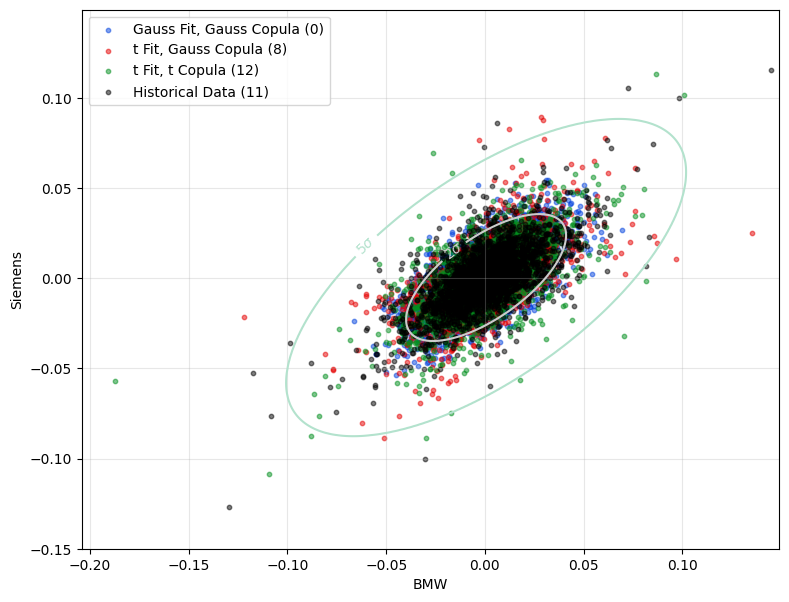
\includegraphics[width=0.7\textwidth]{figures/5_sigma_contour_simulation}
\caption{Distribution of the daily returns of BMW and Siemens stock price from 2010 to 2022 (black points), Gaussian copula simulation (green points), and t-student copula simulation (red points). The red and blue lines represent the $2$ and $5\sigma$ contours.}
\label{fig:5sigma_contour}
\end{figure}

Just \emph{counting} the number of events outside the $5\sigma$ contour it is apparent how the Gaussian copula severely underestimate extreme market shocks (actually there few events already outside the $2\sigma$).

%\subsection{Copula Types}
%There are numerous types of copula but two are the main classes: one-factor and two-factor copulas.
%The most popular one-factor copulas are the Gaussian and the Archimedean. The latter can be split further into Gumbel, Clayton, and Frank copulas.
%Two-factor copulas include the student’s t, Frechet, and Marshal-Olkin copula. 
%We are going to concentrate on the Gaussian copula only though.

\subsection{Correlated Defaults}

Let's now apply the copula to estimate the probability of simultaneous default in the case of correlated assets.
Consider 10 firms with 10\% default probability each and compute the probability of having 5 defaults within the next year when the assets are perfectly correlated ($\rho=1$).
%Imagine a company with probability of defaulting within the next year equal to $\Pdef$.
%
%To simulate the credit event by Monte Carlo it can be thrown a random number from a uniform distribution between 0 and 1  then:
%\begin{itemize}
%\item if it is lower or equal to $\Pdef$ then there has been default;
%\item if it is higher no default happened.
%\end{itemize}

\pythoncodenon{code/modelling_risk_3.py}

%In such a way we have a "successful" experiment with the desired probability.

\begin{ioutput}
Simulated defaults (first 5 scenarios):
[[0. 0. 0. 0. 0. 0. 0. 0. 0. 0.]
[0. 0. 0. 0. 0. 0. 0. 0. 0. 0.]
[0. 0. 0. 0. 0. 0. 0. 0. 0. 0.]
[0. 0. 0. 0. 0. 0. 0. 0. 0. 0.]
[0. 0. 0. 0. 0. 0. 0. 0. 0. 0.]]

Total defaults per simulation:
[0. 0. 0. 0. 0.]

Simulation with >= 5 defaults:
[0 0 0 0 0]

P(ndefs >=5|rho=1): 0.100436
\end{ioutput}

The estimated probability is correctly about 10\% indeed given the perfect correlation either there is no default or five "simultaneous" defaults with probability equal to marginal probability $P_i = 0.1$.
This is very different from the result obtained in the case of independent defaults (see Sec.~\ref{sec:credit_event_simulation}) where the final probability was roughly 
$$
0.1^5 \cdot 0.9^5\cdot 252 \approx 0.0015
$$


%
%In this case the result is close to 10\%, like we had only one single company defaulting. 
%Indeed given the perfect correlation either there is no default or three "simultaneous" defaults with 10\% probability.

%To generate samples from correlated distributions it is enough to determine the copula function as described in the previous Section. At the end of the computation each component of the sample is now converted to a set of random numbers drawn from the proper joint distribution.
%
%Imagine three companies ($A$, $B$ and $C$) which have a cumulative probability of defaulting within the next two years of 10\%.
%Let's compare the probability to have the three of them all defaulting within the next two years in two cases: independent and perfectly correlated default probabilities.
%
%\pythoncodenon{code/modelling_risk_6.py}
%
%In the first case (independent probabilities), the odds to get three defaults within two years is equivalent to the product of the single probabilities, hence $P_{\mathrm{uncorr}} = 10\% \cdot 10\% \cdot 10\% = 0.1 \%
%$.
%
%\begin{ioutput}
%Uncorrelated defaults
%3D copula distribution (first two samples only)
%[[0.91972954 0.72719545 0.95619535]
% [0.7409053  0.81691954 0.5108085 ]]
%Measured P_def: 0.00096
%\end{ioutput}
%
%If we repeat the same Monte Carlo experiment with perfectly correlated default probabilities we have (notice that the covariance matrix has non-diagonal 0.99999999 entries to avoid numerical errors, they should be 1)
%
%In this case the result is close to 10\%, like we had only one single company defaulting. 
%Indeed given the perfect correlation either there is no default or three "simultaneous" defaults with 10\% probability.
%
%\begin{ioutput}
%Correlated defaults
%3D copula distribution (first two samples only)
%[[0.94531087 0.94533677 0.94534905]
% [0.3477901  0.347964   0.3478019 ]]
%Measured P_def: 0.10233
%\end{ioutput}


%\subsubsection{Independent Defaults}\label{independent-defaults}
%
%If the default times of the number of companies are independent,
%default probabilities can be
%calculated through multiplication and integration of the single default
%probability curves without Monte Carlo simulation.
%
%As an example, consider the probability to have two defaults among four
%companies. Let \(\tau_i\) be the default time of name \(i\) and \(F_i(t)\)
%its distribution. Then the probability that name 1 defaults second in
%the basket before time \(t\) is:
%
%\begin{equation}
%\begin{split}
%&\mathbb{P}((\tau_2\lt\tau_1)\cap (\tau_1\lt t)\cap (\tau_1\lt\tau_3)\cap (\tau_1\lt\tau_4)) +\\
%&\mathbb{P}((\tau_3\lt\tau_1)\cap (\tau_1\lt t)\cap (\tau_1\lt\tau_2)\cap (\tau_1\lt\tau_4)) =\\
%&\int_0^t{F_2 (s)\cdot (1-F_3 (s)) \cdot (1-F_4 (s))~dF_1(s)} +  \int_0^t{F_3 (s)\cdot (1-F_2 (s)) \cdot (1-F_4 (s))~dF_1(s)}
%\end{split}
%\label{eq:indep_default}
%\end{equation}
%
%Suppose the default probabilities of three companies, $A$, $B$ and $C$ are
%given as in the following table (in each interval are linear):
%
%\begin{center}
%	\begin{tabular}{|c|c|c|c|}
%		\hline
%		time in years & A & B & C \\
%		\hline
%		\hline
%		0 & 0 & 0 & 0 \\
%		1 & 0.022032 & 0.0317 & 0.035 \\
%		2 & 0.046242 & 0.0655 & 0.075 \\
%		3 & 0.07266 & 0.1022 & 0.121 \\
%		4 & 0.101233 & 0.142 & 0.153 \\
%		5 & 0.131885 & 0.1752 & 0.205 \\
%		\hline
%	\end{tabular}
%\end{center}
%and suppose that the default events of the three companies are
%independent. The integral in Eq.~\ref{eq:indep_default} can be solved by substitution:
%
%\[ \int_{x_0}^{x_1}{(1-F_B(x))(1-F_C(x))dF_A(x)}\]
%
%Setting \(t=m_A x + q_A\) it becomes:
%
%\[ \int_{m_A x_0 + q_A}^{m_A x_1 + q_A}{(1-F_B(x(t)))(1-F_C(x(t)))dt}\qquad\Big(\textrm{with}~x(t) = \cfrac{t -q_A}{m_A}\Big) \]
%and similarly for company $B$ and $C$.
%
%To convert it into \texttt{python} we can use \texttt{scipy.integrate.quad} to
%perform the integral and \texttt{numpy.interp} to determine the
%intermediate default probabilities.	
%	First to default prob at time (1) for company A: 0.02131
%	First to default prob at time (2) for company A: 0.04301
%	First to default prob at time (3) for company A: 0.06460
%	First to default prob at time (4) for company A: 0.08573
%	First to default prob at time (5) for company A: 0.10606
%	First to default prob at time (1) for company B: 0.03080
%	First to default prob at time (2) for company B: 0.06160
%	...
%	\end{Verbatim}
%\end{tcolorbox}

%\section{Cholesky Transformation to Correlate Variables}
%In Section~\ref{sec:cholesky} it has been shown that a given matrix, $[\Sigma]$ can be factored uniquely into a product $[\Sigma]=[L]^T [L]$, where $[L]$ is a lower triangular matrix with positive diagonal entries. The matrix $[L]$ is the Cholesky (or "square root") matrix.
%
%The Cholesky matrix can also be used to correlate random variables. Indeed if $[\Sigma]$ is the covariance matrix of a set of random variables , it transforms them such that their covariances are given by $[\Sigma]$. 
%
%The intuition behind that relies on the following statement: from the transformation properties of the Gaussian distribution it is known that if $X\approx\mathcal{N}(\tau,\Lambda)$ then the transformation $Y=BX+b$ results in $Y$ distributed as $Y\approx\mathcal{N}(B\tau +b,B\Lambda B^{T})$.
%
%Now immagine that $X$ is sampled from a standard $n$-dimensional normal distribution (i.e. $X\approx\mathcal{N}(0,\mathbb{1})$, where $\mathbb{1}$ is the $n\times n$ identity matrix, then $Y=BX+b$ is distributed as $Y\approx\mathcal{N}(b,BB^{T})$, which is just plugging in $\tau=0$ and $\Lambda=\mathbb{1}$ in the relation above.
%
%If you now want $Y$ to be distributed as $Y\approx\mathcal{N}(\mu,\Sigma)$, then you need to choose some transformation matrix $A$, such that $AA^{T}=\Sigma$. A good choice for that is the Cholesky decomposition because it is explicitly structured to fulfill this condition and there are standard functions in lots of libraries which compute it for you.
%
%As a practical example, suppose that $X$ is a vector of independent standard normal variables. The matrix $[L]$ can be used to create a new vector $Z$ such that the covariance of $Z$ equals $[\Sigma]$.
%
%\pythoncodenon{code/modelling_risk_7.py}
%
%\begin{ioutput}
%[[1.73205081 0.        ]
% [0.57735027 0.81649658]]
%\end{ioutput}
%
%Figure~\ref{fig:cholesky_norm} shows the original uncorrelated variable $X$ (left), and the transformed variable $Z$ with correlation $[\Sigma]$ (right).
%
%\begin{figure}[htbp]
%\centering
%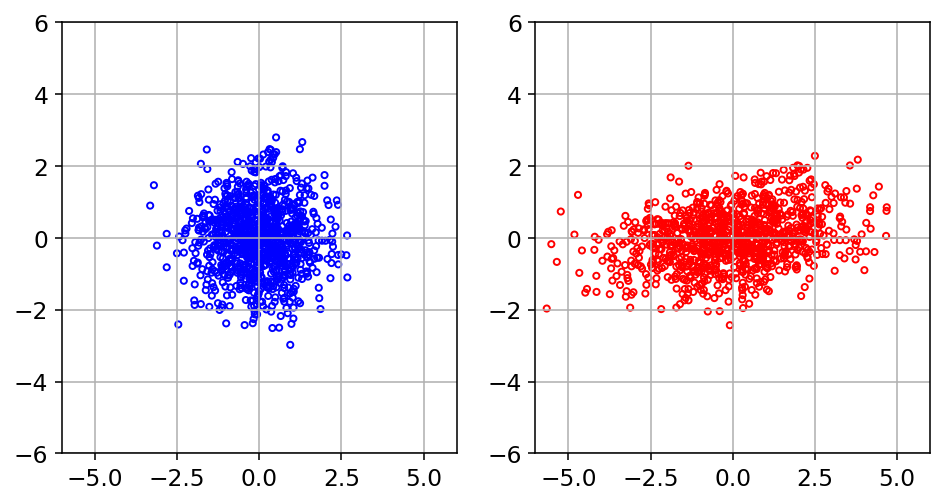
\includegraphics[width=0.7\textwidth]{figures/cholesky_norm}
%\caption{The original uncorrelated variable $X$ (left), the transformed variable $Z$ (right).}
%\label{fig:cholesky_norm}
%\end{figure}
%
%Clearly, if you start with correlated variables, you can apply the Cholesky inverse transformation to get uncorrelated variables.
%If you take the $Z$ points generated above and apply $[L]^{-1}$, the original data is obtained again. Figure~\ref{fig:cholesky_inv} shows the resulting distribution.
%
%\begin{ipythonnon}
%orig_X = np.dot(Z, np.linalg.inv(L))
%\end{ipythonnon}
%
%\begin{figure}[htbp]
%\centering
%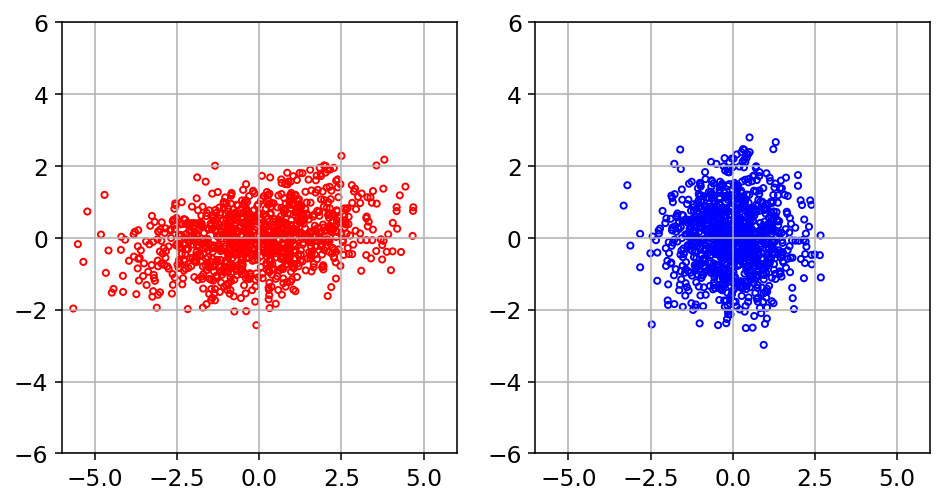
\includegraphics[width=0.7\textwidth]{figures/cholesky_inv}
%\caption{The transformed variable $Z$ (left), and the original data obtained by the application of the inverse Cholesky transformation (right).}
%\label{fig:cholesky_inv}
%\end{figure}

%\subsection{t-copula with $\chi^2$ Method}
%\label{sec:t-student_copula}
%The t-student copula allows a range of dependence structures depending
%on the $\nu$ parameter (the number of degrees of freedom of the t-student function).
%It is a symmetrical copula and has larger tails than the Gaussian. The following algorithm allows to compute it:
%\begin{itemize}
%\item given the correlation matrix $[\Sigma]$ find its Cholesky decomposition $[L]$;
%\item simulate a n-dimensional vector of normal independent identically distributed variables $Y$;
%\item simulate a $\chi^2$ with $\nu$ degrees of freedom $S$;
%\item calculate $Z = \sqrt{\cfrac{\nu}{S}}\cdot [L] \cdot Y$;
%\item finally, $U = CDF_{t-student(\nu)}(Z)$.
%\end{itemize}
%
%\pythoncodenon{code/modelling_risk_8.py}
%
%\begin{figure}[htbp]
%\centering
%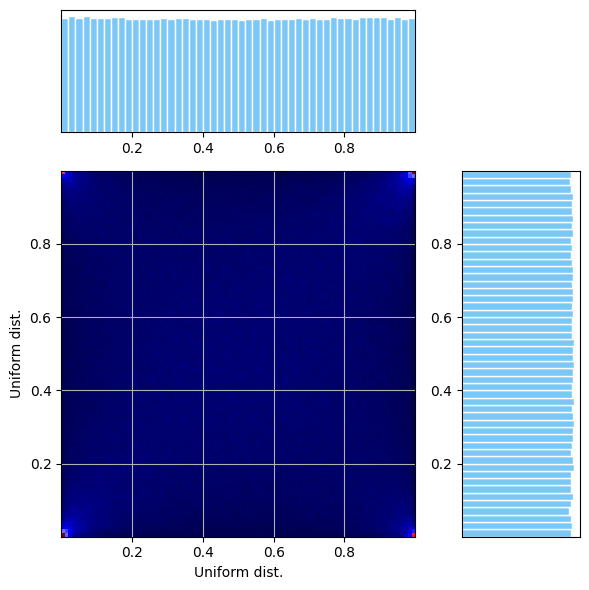
\includegraphics[width=0.45\textwidth]{figures/t-copula_2d}
%\quad
%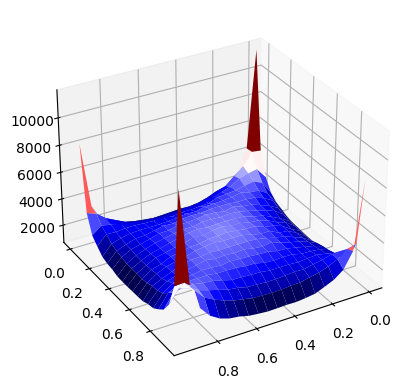
\includegraphics[width=0.5\textwidth]{figures/t-copula_3d}
%\caption{Graphical representations of the t-copula, 2D on the left, 3D on the right.}
%\label{fig:t-copula}
%\end{figure}
%
%\subsection{Copula Types}
%There are numerous types of copula but two are the main classes: one-factor and two-factor copulas.
%The most popular one-factor copulas are the Gaussian and the Archimedean. The latter can be split further into Gumbel, Clayton, and Frank copulas.
%Two-factor copulas include the student’s t, Frechet, and Marshal-Olkin copula. 
%We are going to concentrate on the Gaussian copula only though.

%\section{One Factor Gaussian Copula Model}
%While there are several types of copula function models, the first introduced was the \emph{one-factor Gaussian copula model}. This model is quite simple and has, above all, the advantage that can be solved analytically. 
%
%In essence the one-factor Gaussian copula, is nothing but a numerical algorithm to generate samples of normally distributed random variables that have a given (Gaussian) pair-wise correlation. 
%
%Consider a portfolio of $N$ bonds and assume that the marginal default probabilities are known for each issuer. Define:
%
%\begin{itemize}
%\tightlist
%\item
%$t_i$, the time of default of the $i^{th}$ company:
%\item $Q_i(t)$, the cumulative probability that company $i$ will default before time $t$; that is, the probability that $t_i \le t$.
%\end{itemize}
%
%To generate a one-factor model for the default times ($t_i$) we define random variables $X_i$ $(1\le i \le N)$
%\begin{equation}
%X_i = a_i M + \sqrt{1-a_i^2}Z_i,\qquad i = 1, 2,\ldots, N
%\label{eq:normalized_var}
%\end{equation}
%where $M$ and the $Z_i$ are independent zero-mean unit-variance  distributions (hence $X_i$ are also distributed with zero-mean and unit standard-deviation) and $-1 \le a_i < 1$.
%
%Eq.~\ref{eq:normalized_var} defines a correlation structure between the $X_i$ which are dependent on a single common factor $M$. The $Z_i$ term is called the \emph{idiosyncratic component} of default. The particular functional form of Eq.~\ref{eq:normalized_var} has been chosen to ensure the desired correlation structure among the $X_i$. Indeed the correlation between $X_i$ and $X_j$ is
%
%\begin{equation*}
%\rho(X_i, X_j) = \cfrac{\mathbb{E}[(X_i-\mu_i)(X_j-\mu_j)]}{\sigma_{i}\sigma_{j}} = \mathbb{E}[X_i X_j] = a_i a_j \mathbb{E}[M^2] = a_i a_j
%\end{equation*}
%where we just exploit the definition of $X_i$ and its properties.
%
%%Assume that the $i^{th}$ company has defaulted by the time $t_i$ if $X_i$ is below a threshold value $\bar{x}_i(t_i)$.
%If $F_i$ is the cumulative distribution function of $X_i$, with an inverse transform (see Sec.~\ref{sec:distribution-transformation}) we can map $X_i$ to $t_i$, so that $Q_i(t_i) = P(X_i\le x)=F_i(x)$. Therefore a point $X_i = x$ is transformed to $t_i = t$ with $x = F_i^{-1}[Q_i(t)]$ connecting the marginal distribution of the copula model to the default times.
%
%Let's note that, \textbf{conditional} on $M$, the $N$ default events are \textbf{independent}. So we can write
%\begin{equation}
%\begin{split}
%Q_i^{\textrm{corr}}(t_i|M) = P(X_i\le x|M) &= P(a_i M + \sqrt{1-a_i^2}Z_i\le x) =\\
%&= P\left(Z_i\le \cfrac{x-a_i M}{\sqrt{1-a_i^2}}\right)
%=H_i\left(\cfrac{F^{-1}[Q(t_i)]-a_i M}{\sqrt{1-a_i^2}}\right)
%\end{split}
%\label{eq:generic_copula}
%\end{equation}
%where $H_i$ is the cumulative distribution function of the $Z_i$.
%
%Although in principle any distribution could be used for $M$ and the $Z$'s (provided they have zero mean and unit variance), one common choice is to let them be standard normal distributions (resulting in a Gaussian copula).
%So we can rewrite Eq.~\ref{eq:generic_copula} as
%
%\begin{equation}
%Q_i^{\textrm{corr}}(t_i|M) = \Phi\left(\cfrac{\Phi^{-1}[Q(t_i)]-a_i M}{\sqrt{1-a_i^2}}\right)
%\label{eq:gaussian_one_factor_copula}
%\end{equation}
%where $\Phi$ denotes the standard normal cumulative distribution function.
%
%If we call $\mathcal{C}(t_1,\ldots,t_N)$ the joint distribution of the default times of the $N$ bonds in the portfolio then
%
%\begin{equation}
%\mathcal{C}(t_1,\ldots,t_N, \rho)=\Phi_{N}(\Phi^{-1}(Q_1(t_1)),\ldots,\Phi^{-1}(Q_N(t_N)), \boldsymbol{\rho})
%\label{eq:gaussian_copula}
%\end{equation}
%where $\boldsymbol{\rho}$ represents the correlation matrix of the default probabilities. Eq.~\ref{eq:gaussian_copula} is the one factor Gaussian copula model (one factor because there is only a random variable, $M$, which determines the correlation between $X_i$).
%
%Different distribution choices result in different copula models, and in various natures of the default dependence. For example, copulas where the $M$ have heavy tails, generate models where there is a greater likelihood of a early defaults clustering for several companies.
%
%\subsubsection{Standard Market Model}
%\label{standard-market-model}
%
%Consider the following two assumptions:
%
%\begin{itemize}
%\tightlist
%\item all the companies have the same default intensity (hazard rates), i.e, $\lambda_i = \lambda$ (which means they all have the same default probabilities $Q_i = Q$);
%\item the pairwise default correlations are the same, i.e $a_i = a$; in other words the contribution of the market component $M$ is the same for all the companies and the correlation between any two companies is constant, $\rho = a^2$.
%\end{itemize}
%
%Given the market situation $M = m$, all companies have the same cumulative default probability $Q_i^{\textrm{corr}}(t_i|m)=P(X_i < x|m)$. 
%
%In this case the one factor Gaussian model is also called \emph{Market Standard Model}. Later in this Notes we will also see how the correlation used in Eq.~\ref{eq:gaussian_one_factor_copula} can be implied from the market quotes of credit derivatives.
%
%Letting $l(t|m)$ be the total defaults that have occurred by time $t$ conditional on the market condition $M = m$, then $l(t|m)$ follows a binomial distribution (see Appendix~\ref{binomial-distribution}), and the probability of default of $j$ companies can be expressed as
%
%\begin{equation}
%P_{\mathrm{def}}(l(t|m) = j) = \cfrac{N!}{j!(N-j)!}(Q_i^{\textrm{corr}}(t_i|m))^j(1-Q_i^{\textrm{corr}}(t_i|m))^{N-j},\qquad  j=0, 1, 2,\ldots,N
%\end{equation}
%
%In general to evaluate any function $g(P_{\mathrm{def}}[l(t)])$ regardless the value of one its factor ($M$) (e.g. an NPV or a fair value), is necessary to average according to all possible values that this factor can take. The average is performed by integrating over the market factor (i.e. this is equivalent to perform a weighted sum of $g$ with the probability distribution of the factor).  
%
%\begin{equation}
%g(P_{\mathrm{def}}(l(t) = j)) = \int_{-\infty}^{\infty}{g(P_{\mathrm{def}}[l(t|m) = j])\cdot f_M(m)dm}
%\label{eq:gaussian_quadrature}
%\end{equation}
%
%In the general case where the default probabilities of each company are not the same it is possible to determine $P_{\mathrm{def}}[l(t|M)=j]$ through an iterative procedure before proceeding with the integration of Eq.~\ref{eq:gaussian_quadrature}. An example of this iterative technique will be shown in Section~\ref{sec:expected_losses}.
%
%\subsection{Extensions of the One Factor Copula Model}
%Many other one-factor model have been studied: t-Student copula, Clayton copula,\ldots In general we can define a new model by simply choosing particular functional forms for $M$ and $Z_i$ in Eq.~\ref{eq:normalized_var} provided they are with zero mean and standard deviation one. 
%
%If instead of the single factor $M$ there are two or more, Eq.~\ref{eq:normalized_var} becomes
%
%\begin{equation}
%X_i = a_1 M_1 + a_2 M_2 + \sqrt{1 - a_1^2 - a^2_2}Z_i
%\end{equation}
%and similarly
%\begin{equation}
%Q^{\textrm{corr}}(t|M_1, M_2) = \Phi\left(\cfrac{\Phi^{-1}[Q(t)]-a_1 M_1 - a_2 M_2}{\sqrt{1 - a_1^2 - a^2_2}}\right)
%\end{equation}
%In terms of computation time, this kind of models are proportionally slower with the increase of the factor numbers, since the integration of Eq.~\ref{eq:gaussian_quadrature} has to be carried on each factor of the model.

\section{Basket Default Swaps}
\label{basket-default-swaps}

A Basket Default Swaps (BDS) is a credit derivative on a portfolio of reference entities.

This kind of contracts are very similar to normal CDS except for the protection they offer. With respect to a basket of reference entities, a first-to-default BDS provides insurance for only the first default, a second-to-default BDS provides insurance for only the second default, or a nth-to-default BDS provides insurance for only the $n^{th}$ default. 

For example, in the latter, the seller does not make any payment to the protection buyer for the first $n-1$ defaulted entities, and makes it only for the $n^{th}$. Once there has been this payment the swap terminates.

The cost of protection in nth-to-default basket is obviously dependent on default correlations. Suppose that a basket of 100 reference entities is used to define a 5-year nth-to-default swap and that each reference entity has a 2\% probability of defaulting during the next 5 years. When the default correlation between the reference entities is zero (i.e. they are uncorrelated), the binomial distribution shows that the probability of one or more defaults during 5 years is 86.74\% and the probability of ten or more defaults is 0.0034\%.

A first-to-default is therefore quite valuable whereas a tenth-to-default swap is worth almost nothing.

As the default correlation increases the probability of one or more defaults declines but that for ten or more defaults increases too. In the limit where default correlations are perfect the probability of one or more defaults equals the probability of ten or more and it is 2\%. This is because in this extreme situation the reference entities are essentially the same: either they all default (with 2\% probability) or none of them default (with 98\% probability). Similarly for the value of the basket default swaps.

We now present some numerical results for a nth-to-default basket with two complementary approaches. We assume that principals and expected recovery rates are the same for all underlying reference assets. 

The valuation procedure is similar to that for a regular CDS. There it was based on the probability that a default occurred between times $t_1$ and $t_2$, see Section~\ref{sec:cds_valuation}. Here instead it will rely on the probability that the $n^{th}$ default happened between times $t_1$ and $t_2$. The buyer of protection makes quarterly payments at a specified rate until the $n^{th}$ default occurs, in which case the seller pays $F\cdot(1-R)$, or the end life of the contract is reached. 

Two complementary approaches are going to be presented, each with different ways to compute the default probabilities to construct the needed credit curve.

\subsection{Basket Default Swaps Valuation (Monte Carlo)}
\label{basket-cds-valuation-with-monte-carlo}

\begin{finmarkets}
	In the following we develop a \texttt{BasketDefaultSwaps} class that is able to valuate the basket NPV using a Monte Carlo approach relying on a numerical multivariate Gaussian copula. 
	The logic of the class relies on computing the contract NPV of the contract using a provided discount curve and the appropriate credit curve determined as described above.
\end{finmarkets}

\pythoncodenon{code/credit_derivatives_1.py}

Consider a 2-years 3rd-to-default basket of 10 reference entities, with a spread of 1\%, in the situation where the Gaussian copula correlation varies between is 0.3, the expected recovery rate, $R$, is $40\%$, and the term structure of interest rates is assumed to be flat at 5\%. The default probabilities $Q(t)$ for the ten entities are generated by Poisson processes, see Sec.~\ref{sec:poisson_process}, with constant default intensities, $\lambda_i=0.06$, such that $Q(t) = 1 - e^{-\lambda t}$

\pythoncodenon{code/credit_derivatives_2.py}
\begin{ioutput}
NPV: -0.0129
\end{ioutput}

Using the \texttt{BasketDefaultSwaps} class it is possible to check how the value (and the spread) of such BDS varies as a function of the correlation $\rho$ and the number of defaults (\texttt{n\_defaults}).

Figures~\ref{fig:bds_value_mc} show the resulting distributions. A 1st-to-default is quite valuable for independent defaults, then as correlation increases its value decreases down to the minimum for $\rho=1$.
Other BDS with higher number of required defaults, are less valuable when the default probability is low but increase with correlation. Anyway all of them reach the asymptotic value for $\rho=1$ where all the reference assets act as a single name and can only default all together.

Notice the jiggling nature of each curve in Fig.~\ref{fig:bds_value_mc} (left) this is due to the fluctuation in the results due to Monte Carlo approximation (i.e. finite sampling).

\begin{figure}[htb]
	\centering
	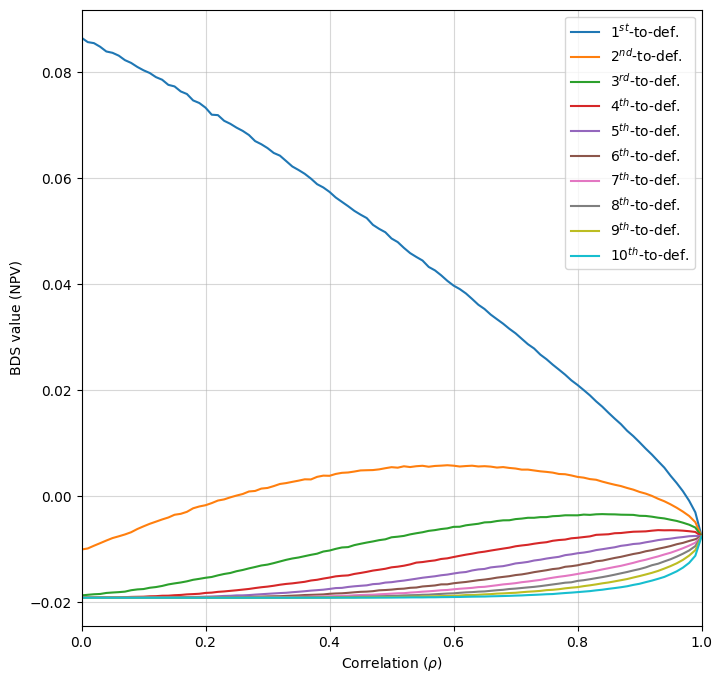
\includegraphics[width=0.45\textwidth]{figures/bds_value_mc}
	\quad
	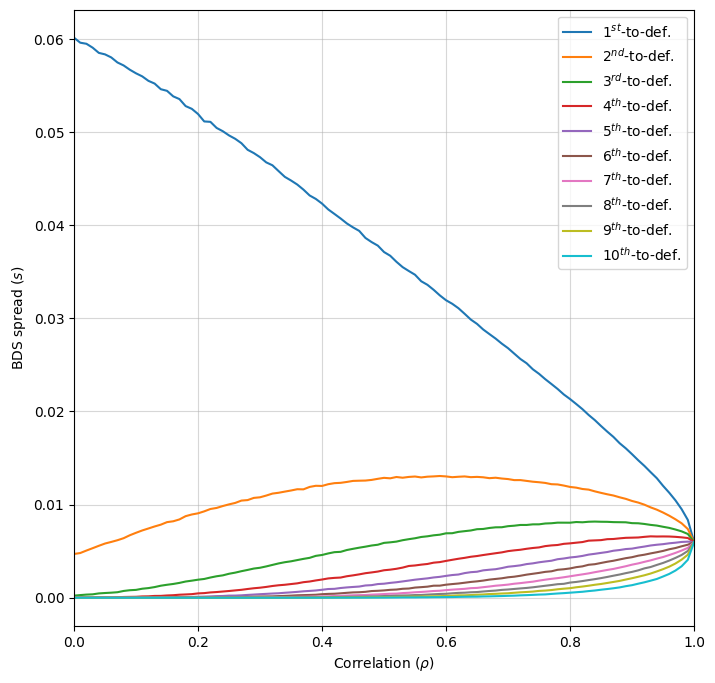
\includegraphics[width=0.45\textwidth]{figures/bds_spread_mc}
	\caption{BDS value (left) and spread (right) as a function of the default correlation $\rho$ and the number of required defaults, using Monte Carlo simulation to determine the credit curve.}
	\label{fig:bds_value_mc}
\end{figure}

\section{Complex Correlation Structures and the Financial Crisis}
\label{complex-correlation-structures-and-the-financial-crisis}

In the derivation of the Gaussian Copula Model we have used the normal distribution. However, we could have used other and more complex copulas as well. For example we might want to assume the correlation is non-symmetric which is useful in finance when correlations become very strong during market crashes and returns very negative.

In fact, Gaussian copulas are said to have played a key role in the 2008 financial crisis as tail-correlations were severely underestimated. Consider a set of mortgages in a CDO (a kind of derivative that will be described in the next Chapter): they are clearly correlated, since if one mortgage fails, the likelihood that another failing is increased. In the early 2000s, the banks only knew how to model the marginals of the default rates. Then an (in)famous paper by Li~\cite{bib:copula_li} suggested to use Gaussian copulas to model the correlations between those marginals. Rating agencies relied on this model so heavily, that severely underestimated the risk and gave false ratings\ldots

If you are interested in the argument read this paper~\cite{bib:copula_and_2008} for an excellent description of Gaussian copulas and the Financial Crisis, which argues that different copula choices would not have made a difference but instead the assumed correlation was way too low.

\section*{Exercises}
\begin{question}
Using the \emph{probability integral transform} morph a Gumbel distribution into a Gaussian. Plot also all the distributions involved in the transformation.
\end{question}

\cprotEnv\begin{solution}
\begin{ipython}
from scipy.stats import gumbel_l, norm
from matplotlib import pyplot as plt

gumbel = gumbel_l()
xg = gumbel.rvs(100000)
xu = gumbel.cdf(xg)
xn = norm.ppf(xu)

sub1 = plt.subplot(1, 3, 1)
sub1.hist(xg, 50)
sub1.grid(True)
sub1.set_xlabel("$x_{gumbel}$")
sub2 = plt.subplot(1, 3, 2)
sub2.hist(xu, 50)
sub2.grid(True)
sub2.set_xlabel("$x_{uniform}$")
sub3 = plt.subplot(1, 3, 3)
sub3.hist(xn, 50)
sub3.grid(True)
sub3.set_xlabel("$x_{normal}$")
plt.show()
\end{ipython}

\begin{figure}[htbp]
\begin{center}
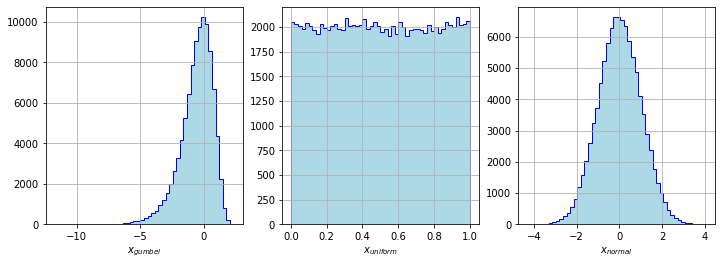
\includegraphics[width=0.9\linewidth]{figures/ex_gumbel_to_gauss.png}
\end{center}
\end{figure}
\end{solution}

\begin{question}
Without using the corresponding \texttt{rvs()} method try to generate 10 random numbers distributed as a Beta distribution with parameters \texttt{a=3} and \texttt{b=10}.

\noindent\textbf{Hint:} starts with generating uniformly distributed random numbers.
\end{question}	

\cprotEnv\begin{solution}
\begin{ipython}
from scipy.stats import beta, uniform

x = uniform.rvs(size=10)
b = beta(a=3, b=10)
x_b = b.ppf(x)

print (x_b)
\end{ipython}
\begin{ioutput}
[0.29190237 0.45669406 0.10336582 0.5403107 0.08305872 0.32425694
0.43902811 0.11820592 0.28659784 0.22316621]
\end{ioutput}
\end{solution}

\begin{question}
Consider two companies whose default probabilities as a function of time are modeled according to a log-normal distribution with $\sigma=0.5$ (\texttt{scipy.stats.lognorm(0.5)}). Compare the joint 2D distributions in case of no correlation and with a Gaussian correlation of 0.8.

\noindent\textbf{Hint:} to plot the joint distribution use \texttt{matplotlib} function \texttt{hist2d(x1, x2, range=[[x1min, x1max], [xmin, x2max]], bins=(50, 50)) }.
\end{question}

\cprotEnv\begin{solution}
\begin{ipython}
from scipy.stats import lognorm, multivariate_normal, norm
import numpy

numpy.random.seed(1)
samples = 1000000
l1_uncorr = lognorm(0.5).rvs(size=samples)
l2_uncorr = lognorm(0.5).rvs(size=samples)
mvnorm = multivariate_normal(mean = (0, 0), 
                             cov = [[1, 0.8],
                                    [0.8, 1]])
x = mvnorm.rvs(size=samples)
x_corr = norm.cdf(x)
l1_corr = lognorm(0.5).ppf(x_corr[:, 0])
l2_corr = lognorm(0.5).ppf(x_corr[:, 1])

plt.figure(figsize=(12, 4))
sub1 = plt.subplot(1, 2, 1)
sub1.hist2d(l1_uncorr, l2_uncorr, range=[[0, 2], [0, 2]], bins=(100, 100))
sub2 = plt.subplot(1, 2, 2)
sub2.hist2d(l1_corr, l2_corr, range=[[0, 2], [0, 2]], bins=(100, 100))
plt.show()
\end{ipython}
\noindent 
The resulting comparison is shown in Fig.~\ref{fig:joint_2d}.
\begin{figure}[htbp]
\begin{center}
	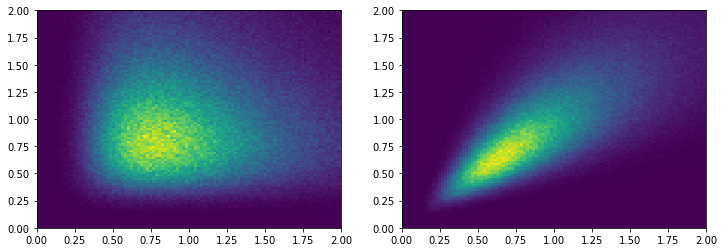
\includegraphics[width=0.9\linewidth]{figures/copula_lognormal.png}
\end{center}
\caption{Comparision of the joint 2D distributions in case of no correlation (left) and with a Gaussian correlation of 0.8 (right).}
\label{fig:joint_2d}
\end{figure}

In order to quantify the difference between the two cases, calculate the probability that both companies default in the next six months.

The probability that a single company defaulted in six months regardless the other can be calculated from the \texttt{cdf} of the log-normal distribution. Hence in case of independent probabilities is just required the squared of this value (about 0.07\%).

\begin{ipython}
default_6m = lognorm(0.5).cdf(.5)
print(default_6m**2)
\end{ipython}
\begin{ioutput}
0.006860563560014724
\end{ioutput}

In case of correlation instead we have to loop over the samples from the joint multivariate distribution and check how many times both values are less than \texttt{default\_6m}. Here two approaches are shown: the traditional one with a for-loop and a \emph{one-liner} using \texttt{numpy.array}.

\begin{ipython}
#success = 0.0
#for i in range(samples):
#    if max(x_corr[i]) < default_6m:
#        success += 1

success = len(x_corr[np.max(x_corr, axis=1) < default_6m])
print (success/samples)
\end{ipython}
\begin{ioutput}
0.044654
\end{ioutput}

This result can be interpreted graphically by saying that the entries in the "square" $[0, 0.5]$ in the left histogram are about 0.7\% of the total while the entries in the right plot in same "square" are about 4.5\% of the total. 
\end{solution}

\begin{question}
Imagine a risk manager which owns two non-investment graded bonds (e.g. rated BB+ and BB respectively). The bonds have been issued by two companies and their yearly default probabilities ($P_{\mathrm{def}}$) are as listed below:

\begin{table}[htbp]
\centering
\begin{tabular}{|c|c|c|}
\hline
Time & $P_{\mathrm{def}}$ Asset 1 & $P_{\mathrm{def}}$ Asset 2 \\
\hline
\hline
1 & 0.065 & 0.238 \\
2 & 0.081 & 0.152 \\
3 & 0.072 & 0.113 \\
4 & 0.064 & 0.092 \\
5 & 0.059 & 0.072 \\
\hline
\end{tabular}
\end{table}

How can a a copula be constructed to estimate the joint default probability of these two companies in the next year, assuming a Gaussian default correlation of $\rho_M = 0.4$ ?
\end{question}

\cprotEnv\begin{solution}
It is possible to map the cumulative default probabilities of each asset to the standard normal distribution via $F^{-1}[Q(t)]$.
\texttt{cumsum} can be used to determine $Q(t)$ from the inputs.

\begin{ipython}
import numpy as np
from scipy.stats import norm

PDF1 = np.array([0.065, 0.081, 0.072, 0.064, 0.059])
PDF2 = np.array([0.238, 0.152, 0.113, 0.092, 0.072])

C1 = PDF1.cumsum()
C2 = PDF2.cumsum()

for c in C1:
    print (f"{c:.3f} -> {norm.ppf(c):.4f}")
print ("")
for c in C2:
    print (f"{c:.3f} -> {norm.ppf(c):.4f}")
\end{ipython}
\begin{ioutput}
0.065 -> -1.5141
0.146 -> -1.0537
0.218 -> -0.7790
0.282 -> -0.5769
0.341 -> -0.4097

0.238 -> -0.7128
0.39 -> -0.2793
0.503 -> 0.0075
0.595 -> 0.2404
0.667 -> 0.4316
\end{ioutput}

\begin{table}[htbp]
\centering
\begin{tabular}{|c|c|c|c|c|c|c|}
\hline
Time & $P_{\mathrm{def}}$ Asset 1 & $Q_{\textrm{BB+}}(t)$ & $F^{-1}[Q_{\textrm{BB+}}(t)]$ & $P_{\mathrm{def}}$ Asset 2 & $Q_{\textrm{BB}}(t)$ & $F^{-1}[Q_{\textrm{BB}}(t)]$\\[5 pt]
\hline
\hline
1 & 0.065 & 0.065 & -1.5141 & 0.238 & 0.238 & -0.7128\\
2 & 0.081 & 0.146 & -1.0537 & 0.152 & 0.39 & -0.2793\\
3 & 0.072 & 0.218 & -0.7790 & 0.113 & 0.503 & 0.0075\\
4 & 0.064 & 0.282 & -0.5769 & 0.092 & 0.595 & 0.2404\\
5 & 0.059 & 0.341 & -0.4097 & 0.072 & 0.667 & 0.4316\\
\hline
\end{tabular}
\end{table}

At this point we can apply the correlation structure $\rho_M$ of the Gaussian multivariate distribution ($M$) to the transformed marginals $F^{-1}[Q_{\textrm{BB+}}(t)]$ and $F^{-1}[Q_{\textrm{BB}}(t)]$.

The joint probability of both companies defaulting within one year can be calculated as

\begin{equation*}
Q(t_{\textrm{BB+}}\leq 1 \cap t_{\textrm{BB}}\leq 1) = M(X_{\textrm{BB+}}\leq -1.5141 \cap X_{\textrm{BB}}\leq -0.7128, \rho=0.4)
\end{equation*}

\begin{ipython}
from scipy.stats import multivariate_normal

g = multivariate_normal(mean=[0,0],
                        cov=[[1, 0.4],
                             [0.4, 1]])

print (g.cdf([-1.5141, -0.7128]))
\end{ipython}
\begin{ioutput}
0.03435364791840133
\end{ioutput}
\noindent
which results to be around 3.4\%. Figure~\ref{fig:copula_no_marginals} shows the joint probability distribution, the number we were looking for is given by the fraction of events delimited by the red lines with respect to the total.

\begin{figure}[htbp]
\centering
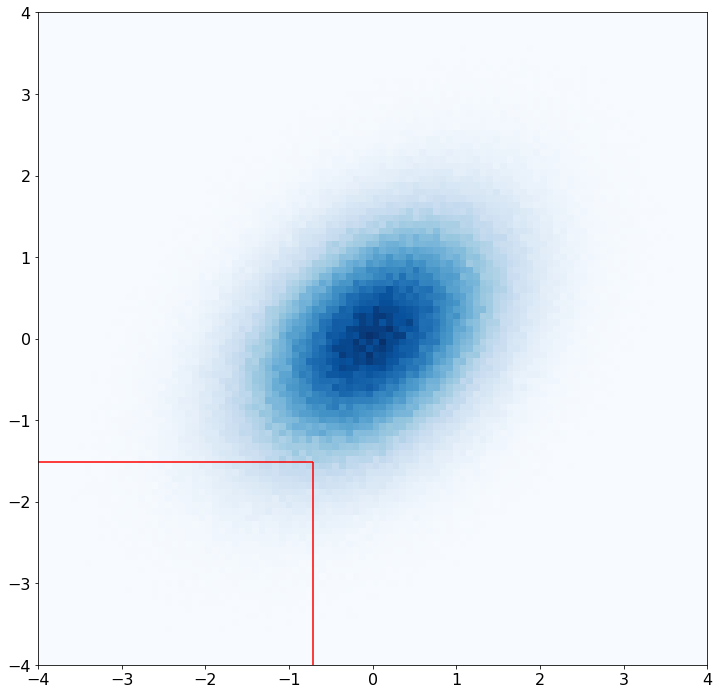
\includegraphics[width=0.5\linewidth]{figures/copula_no_marginals}
\caption{Multivariate Gaussian probability distribution with correlation $\rho=0.4$. The red lines delimited the area representing the default of the two companies within year one.}
\label{fig:copula_no_marginals}
\end{figure}
\end{solution}
 
%\chapter{Credit Derivatives}

A credit derivative is a financial contract that allows parties to minimize their exposure to credit risk. Credit derivatives consist of a privately held, negotiable bilateral contract traded over-the-counter (OTC) between two parties in a creditor/debtor relationship. These allow the creditor to effectively transfer some or all of the risk of a debtor defaulting to a third party. This third party accepts the risk in return for payment, known as the premium.

Credit default swaps have been already introduced in Chapter~\ref{sec:credit-default-swaps}, here two more kind of credit derivatives will be presented: Basket Default Swaps and Collateralized Debt Obligations (CDO).

%\section{Binomial Distribution}
%\label{binomial-distribution}
%
%In statistics, the binomial distribution is a discrete probability of independent events, where each event has exactly two possible outcomes.
%
%For example, if we toss a coin 10 times and we are interested in how many times it will land on heads, the probability of it lending one, two, three, up to 10 head in a row will form a the binomial distribution. 
%
%When we're interested in a specific outcome, let's say 3 heads out of 10 tosses, we call it binomial probability, which is a probability of exactly \(k\) successes on \(n\) repeated trials.
%
%Following the characteristics of this distribution:
%
%\begin{itemize}
%\tightlist
%\item
%  the number of observations or trials is fixed;
%\item
%  each observation or trial is independent. Like in the coin toss, the previous toss doesn't affect the following;
%\item
%  the probability of success is exactly the same from one trial to another. Each coin toss has 50\% chances to fall in heads or tails.
%\end{itemize}
%
%The probability mass function in this case describes the probability of an outcome, and for the binomial distribution is
%
%\begin{equation} \mathrm{PMF}_{\mathrm{binomial}} = \cfrac{n!}{k!(n-k)!}p^k (1-p)^{n-k}
%\label{eq:binomial_pmf}
%\end{equation}
%where \(n\) is the number of observations, \(k\) the desired outcome, \(p\) the probability of an outcome. To have a better understanding of how this formula works let's take a look at two examples.
%
%\subsection{A Fair Coin Flip}\label{a-fair-coin-flip}
%
%If we flip a fair coin 100 times, what is the probability of getting exactly 50 heads ? 
%We might think that since we have equal chances
%of getting heads or tails, the answer would be 50\% probability. On the other hand, what are the odds that we will get 49 heads, or 51 ? Almost 50\% chance too, but what exactly ? 
%
%Let's first answer the first question and then try it for all the possible outcomes to see how our probabilities are distributed. The parameters of the problem are the following: \(n = 100\), \(k = 50\), \(p = 0.5\). Plugging then numbers into Eq.~\ref{eq:binomial_pmf} we get
%
%\begin{equation*}
%P(50) = \cfrac{100!}{50!(100 - 50)!}0.5^{50}(1-0.5)^{(100-50)} \approx 8\%
%\end{equation*}
%
%So there is about an 8\% chance of getting exactly 50 heads on 100 coin tosses. The code below shows how to get this number in \texttt{python}. The probability distribution is shown in Fig.~\ref{fig:binomial_coin_flip}.
%
%\pythoncodenon{code/credit_derivatives_1.py}
%
%\begin{figure}[ht]
%\centering
%    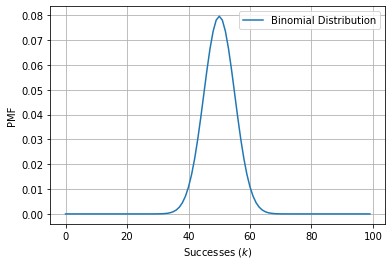
\includegraphics[width=0.7\textwidth]{figures/binomial_2_0.png}
%    \caption{Binomial distribution relative to 100 coin flips.}
%    \label{fig:binomial_coin_flip}
%\end{figure}
%    
%\subsection{Success of Marketing Campaign}
%\label{success-of-marketing-campaign}
%
%In 2014, 8.5\% of adults aged 18 years and older had diabetes. Let's go back to 2014 and pretend we're working for the company that developed a drug for treating diabetes. Our job is to make phone calls to find potential clients. The only statistic we know is that 8.5\% of adults in the US have diabetes. What is the probability that out of 50 calls at least 5 customers have diabetes ? 
%
%Once again let's plug in the numbers into the formula: $n = 50, k > 5, p = 0.085$
%
%\begin{equation*}
%\sum_{k=5}^{n}P(k) = \sum_{k=5}^{n}\Big(\cfrac{50!}{k!(50 - k)!}0.085^{k}(1-0.085)^{(50-k)}\Big) \approx 42.2\%
%\end{equation*}
%there is a 42.2\% chance that out of 50 calls we will find at least five customers with diabetes. Again in \texttt{python} (this time instead of summing PMFs we exploit the binomial CDF, see Fig.~\ref{fig:binomial_cdf})
%
%\pythoncodenon{code/credit_derivatives_2.py}
%
%\begin{figure}[htb]
%\centering
%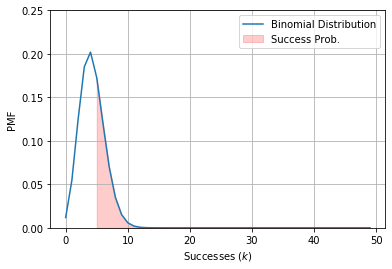
\includegraphics[width=0.7\textwidth]{figures/binomial_5_0.png}
%\caption{Binomial distribution of 50 calls with ($p=0.085$), in red the integrated probability of finding 5 or more successes.}
%\label{fig:binomial_cdf}
%\end{figure}

\section{Basket Default Swaps}
\label{basket-default-swaps}

A Basket Default Swaps (BDS) is a credit derivative on a portfolio of reference entities.

This kind of contracts are very similar to normal CDS except for the protection they offer. With respect to a basket of reference entities, a first-to-default BDS provides insurance for only the first default, a second-to-default BDS provides insurance for only the second default, or a nth-to-default BDS provides insurance for only the $n^{th}$ default. 

For example, in the latter, the seller does not make any payment to the protection buyer for the first $n-1$ defaulted entities, and makes it only for the $n^{th}$. Once there has been this payment the swap terminates.

The cost of protection in nth-to-default basket is obviously dependent on default correlations. Suppose that a basket of 100 reference entities is used to define a 5-year nth-to-default swap and that each reference entity has a 2\% probability of defaulting during the next 5 years. When the default correlation between the reference entities is zero (i.e. they are uncorrelated), the binomial distribution shows that the probability of one or more defaults during 5 years is 86.74\% and the probability of ten or more defaults is 0.0034\%.

A first-to-default is therefore quite valuable whereas a tenth-to-default swap is worth almost nothing.

As the default correlation increases the probability of one or more defaults declines but that for ten or more defaults increases too. In the limit where default correlations are perfect the probability of one or more defaults equals the probability of ten or more and it is 2\%. This is because in this extreme situation the reference entities are essentially the same: either they all default (with 2\% probability) or none of them default (with 98\% probability). Similarly for the value of the basket default swaps.

We now present some numerical results for a nth-to-default basket with two complementary approaches. We assume that principals and expected recovery rates are the same for all underlying reference assets. 

The valuation procedure is similar to that for a regular CDS. There it was based on the probability that a default occurred between times $t_1$ and $t_2$, see Section~\ref{sec:cds_valuation}. Here instead it will rely on the probability that the $n^{th}$ default happened between times $t_1$ and $t_2$. The buyer of protection makes quarterly payments at a specified rate until the $n^{th}$ default occurs, in which case the seller pays $F\cdot(1-R)$, or the end life of the contract is reached. 

Two complementary approaches are going to be presented, each with different ways to compute the default probabilities to construct the needed credit curve.

\subsection{Basket Default Swaps Valuation (Monte Carlo)}
\label{basket-cds-valuation-with-monte-carlo}

\begin{finmarkets}
In the following we develop a \texttt{BasketDefaultSwaps} class that is able to valuate the basket NPV using a Monte Carlo approach relying on a numerical multivariate Gaussian copula. 
The logic of the class relies on computing the contract NPV of the contract using a provided discount curve and the appropriate credit curve determined as described above.
\end{finmarkets}

\pythoncodenon{code/credit_derivatives_1.py}

Consider a 2-years 3rd-to-default basket of 10 reference entities, with a spread of 1\%, in the situation where the Gaussian copula correlation varies between is 0.3, the expected recovery rate, $R$, is $40\%$, and the term structure of interest rates is assumed to be flat at 5\%. The default probabilities $Q(t)$ for the ten entities are generated by Poisson processes, see Sec.~\ref{sec:poisson_process}, with constant default intensities, $\lambda_i=0.06$, such that $Q(t) = 1 - e^{-\lambda t}$

\pythoncodenon{code/credit_derivatives_2.py}
\begin{ioutput}
NPV: -0.0129
\end{ioutput}

Using the \texttt{BasketDefaultSwaps} class it is possible to check how the value (and the spread) of such BDS varies as a function of the correlation $\rho$ and the number of defaults (\texttt{n\_defaults}).

Figures~\ref{fig:bds_value_mc} show the resulting distributions. A 1st-to-default is quite valuable for independent defaults, then as correlation increases its value decreases down to the minimum for $\rho=1$.
Other BDS with higher number of required defaults, are less valuable when the default probability is low but increase with correlation. Anyway all of them reach the asymptotic value for $\rho=1$ where all the reference assets act as a single name and can only default all together.

Notice the jiggling nature of each curve in Fig.~\ref{fig:bds_value_mc} (left) this is due to the fluctuation in the results due to Monte Carlo approximation (i.e. finite sampling).

\begin{figure}[htb]
\centering
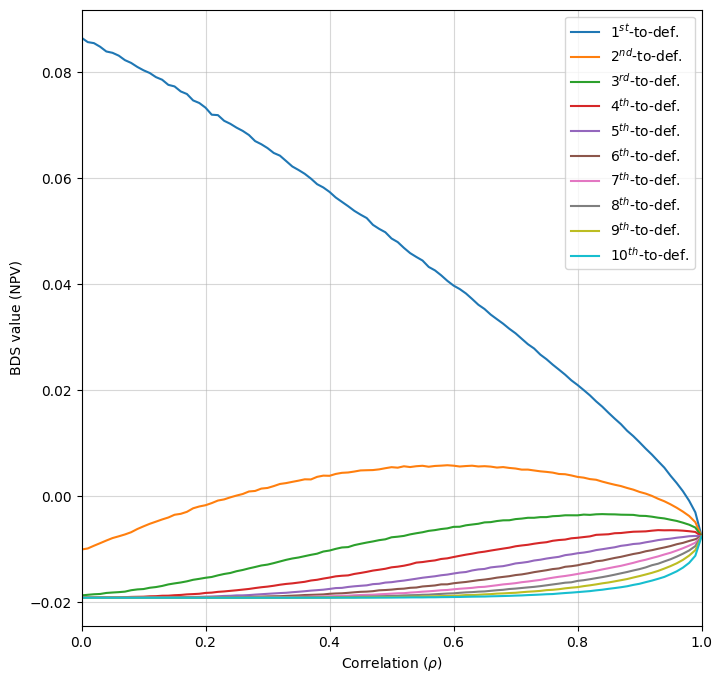
\includegraphics[width=0.45\textwidth]{figures/bds_value_mc}
\quad
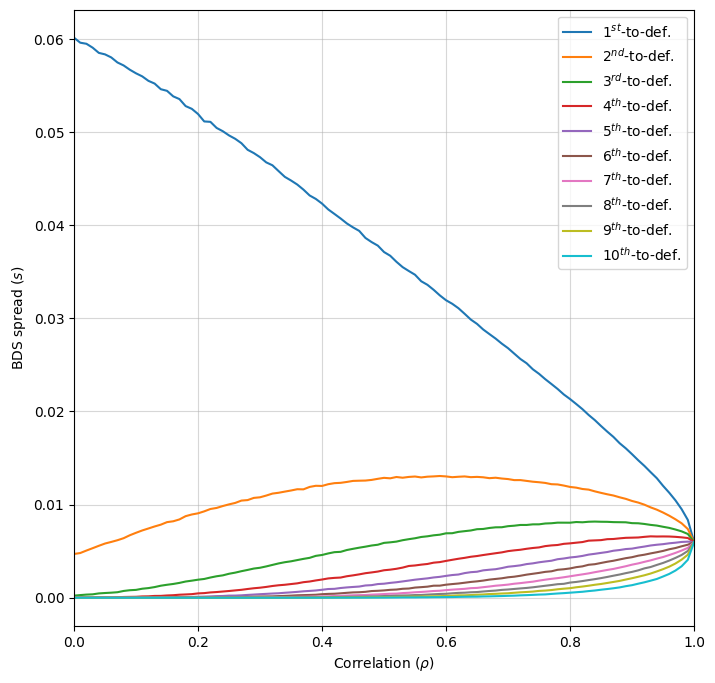
\includegraphics[width=0.45\textwidth]{figures/bds_spread_mc}
\caption{BDS value (left) and spread (right) as a function of the default correlation $\rho$ and the number of required defaults, using Monte Carlo simulation to determine the credit curve.}
\label{fig:bds_value_mc}
\end{figure}

%\subsection{Basket Default Swap Valuation (One Factor Copula Model)}
%\label{basket-cds-valuation-under-market-standard-model}
%
%In this case, since we are under the assumption of the One Factor Copula model, the strategy is:
%\begin{itemize}
%\item compute the correlated default probability of each name according to 
%\begin{equation}
%Q^{\textrm{corr}}(t|M) = \Phi\left(\cfrac{\Phi^{-1}[Q(t)]-\sqrt{\rho} M}{\sqrt{1-\rho}}\right)
%\end{equation}
%\item calculate the probability of having at least $j$ defaults using the binomial distribution
%\begin{equation}
%P_{\mathrm{def}}(l(t|m) \ge j) = \sum_{k=j}^{N}\left[  \cfrac{N!}{k!(N-k)!}Q^{\textrm{corr}}(t|M)^k(1-Q^{\textrm{corr}}(t|M))^{N-k}\right]
%\end{equation}
%\item create a \textbf{credit curve}, $CC(P_{\mathrm{def}})$ according to those probabilities;
%\item re-use the \texttt{CreditDefaultSwap} class to compute NPV and break-even rate with a discount curve $DC$ and the appropriate credit curve determined above, through integration of
%\begin{equation}
%\mathrm{NPV}_{BDS}(DC, CC(P_{\mathrm{def}})) = \int_{-\infty}^{\infty}{\mathrm{NPV}_{CDS}(DC, CC(P_{\mathrm{def}})|M) f_M(m)dm} 
%\end{equation}
%\end{itemize}
%
%To perform the integrals needed by the basket default swap valuation it can be used the method described in Section~\ref{sec:integration}.
%
%\pythoncodenon{code/credit_derivatives_5.py}
%
%Let's repeat a similar scan of the BDS value as a function of the correlation $\rho$ and the number of defaults as performed above. The parameters of the BDS remain unchanged.
%
%\pythoncodenon{code/credit_derivatives_6.py}
%\begin{ioutput}
%0.01791086281290842
%\end{ioutput}
%
%\begin{figure}[htb]
%\centering
%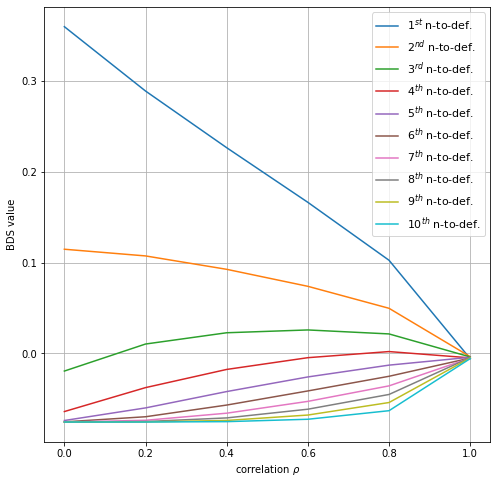
\includegraphics[width=0.5\textwidth]{figures/bds_value_one_factor}
%\caption{BDS value as a function the default correlation $\rho$ and the number of required defaults, under One Factor Gaussian Copula.}
%\label{fig:bds_value_one_factor}
%\end{figure}
%
%Figure~\ref{fig:bds_value_one_factor} shows that the results are close to what obtained with the previous model. It has to be noticed though that the integration performed here is much slower than the simulation with Monte Carlo sampling.

\section{Collateralized Debt Obligation}
\label{collateralized-debt-obligation}

A Collateralized Debt Obligation (CDO) is a credit derivative where the issuer gather risky assets and repackage them into discrete classes, called \emph{tranches}, which are defined on the level of credit risk assumed by the investor. These tranches of securities become the final investment product.

Tranches are named to reflect their risk profile: \emph{senior}, \emph{mezzanine} and \emph{subordinated/equity} and are delimited by an attachment ($L$) and a detachment point ($U$), which represent the percentages of the \textbf{total} principal defining their boundaries. For example, a 5-10\% tranche has an attachment point of 5\% and a detachment point of 10\%. 

Each of these tranches has a different level of seniority relative to the others in the sense that a senior tranche has coupon and principal payment priority over a mezzanine, while a mezzanine tranche has coupon and principal payment priority over an equity one. 

Indeed they receive returns using a set of rules known as \emph{waterfall}. Incomes of the portfolio are first used to provide returns to the most senior tranche, then to the next and so on. So senior tranches are generally safest because they have the first claim on the collateral, although they'll offer lower coupon rates.

It is important to note that a CDO only redistributes the total risk associated with the underlying pool of assets to the priority ordered tranches; it neither reduces nor increases the total risk associated with the pool.

There are various kind of CDOs:
\begin{itemize}
\item in a \textbf{Cash CDO} the reference portfolio consists of corporate bonds owned by the CDO issuer. Cash flows from collateral are used to pay principal and interests to investors. If such cash flows prove inadequate, rewards are paid to tranches according to their seniority. Figure~\ref{fig:cdo_structure} shows a typical structure of a Cash CDO;

\begin{figure}[htb]
\centering
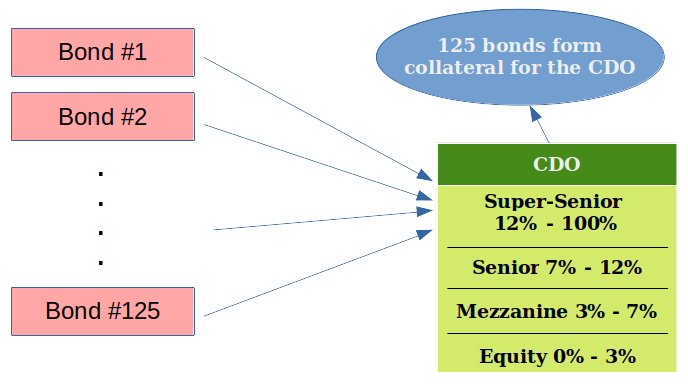
\includegraphics[width=0.7\textwidth]{figures/cdo_structure}
\caption{Typical structure of a Cash CDO, with the reference portfolio made of bonds, which form the contract collateral.}
\label{fig:cdo_structure}
\end{figure}

\item in a \textbf{Synthetic CDO} the underlying reference portfolio is no longer "physical" (e.g. portfolio of bonds or loans), instead it is a \emph{fictitious} portfolio consisting of a number of reference obligations each with an associated notional amount. The value of a synthetic CDO usually comes from insurance premiums of credit default swaps paid for by investors. The investment logic is that sellers assume the underlying assets will perform while investors that will sooner or later default.
\end{itemize}

\subsection{Cash CDO Expected Losses}
\label{sec:expected_losses}

Consider a Cash CDO made of 125 bonds with a maturity of 1 year. Each bond pays a coupon of one unit after 1 year and it has not yet defaulted (the recovery rate $R$ is assumed to be 0). We are interested in the following three tranches: equity ([0, 3] defaults), mezzanine ([4, 6] defaults) and senior ([7, 9] defaults), see Fig.~\ref{fig:cdo_ex_1} (note that in this particular case tranches are identified through the number of defaults and not with principal percentages). 

\begin{figure}[htb]
	\centering
	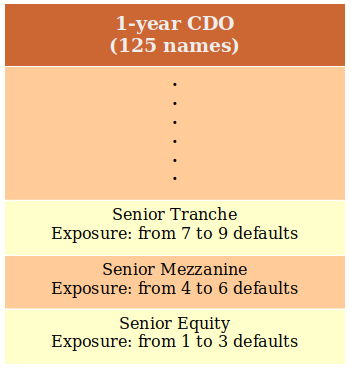
\includegraphics[width=0.5\textwidth]{figures/ex_cdo_1}
	\caption{Structure of the simple Cash CDO considered in the example.}
	\label{fig:cdo_ex_1}
\end{figure}

Assume also that one year default probabilities are identical for each bond ($Q$) and that the correlation between each pair is also identical and equal to $\rho$. Under these assumptions we are in the position to use the Gaussian Copula Model. 

We are interested in the expected losses for each tranche as a function of the correlation $\rho$.

The probability of having $l$ defaults, conditional to the market parameter $M$ will follow a binomial distribution given by
\begin{equation}
p(l|M) = \binom{N}{l}\mathcal{Q}_M^l (1-\mathcal{Q}_M)^{N-l}
\label{eq:def_prob_ex_cdo_1}
\end{equation}
where $N$ is the number of bonds in the portfolio and 
\begin{equation}
\mathcal{Q}_M = \Phi\left(\cfrac{\Phi^{-1}(Q)-\sqrt{\rho}M}{\sqrt{\-\rho}}\right)
\end{equation}
where $\Phi$ is the standard normal CDF and $Q$ the marginal probability of default within 1 year of a single name.

From the definition of each tranche with have that the expected losses are
\begin{itemize}
	\item $\mathbb{E}_{\textrm{equity loss}}(l, \mathcal{Q}_M)=3\cdot p(l\ge 3|M) + \sum_{k=1}^{2}k\cdot p(l=k|M)$
	\item $\mathbb{E}_{\textrm{mezzanine loss}}(l, \mathcal{Q}_M)=3\cdot p(l\ge 6|M) + \sum_{k=1}^{2}k\cdot p(l=k+3|M)$
	\item $\mathbb{E}_{\textrm{senior loss}}(l, \mathcal{Q}_M)=3\cdot p(l\ge 9|M) + \sum_{k=1}^{2}k\cdot p(l=k+6|M)$
\end{itemize}
	
Each probability can be calculated by integrating the above with respect to $M$
	
\begin{equation} 
\mathbb{E}_{\mathrm{tranche}} = \int_{-\infty}^{\infty}{\mathbb{E}_{\mathrm{tranche}}(l, \mathcal{Q}_M) f_M(m)dm}
\end{equation}

Let's see the corresponding \texttt{python} implementation.

\pythoncodenon{code/credit_derivatives_7.py}

We define a function \texttt{p} which implements the expected losses for each tranche according to Eq.~\ref{eq:def_prob_ex_cdo_1}.
The function depends on the parameter \texttt{M}, and takes as inputs the correlation \texttt{rho} and the tranche attach-detach limits.
Finally we loop over a range of possible values for the correlation on each tranche to draw the plot of the expected losses vs correlation, shown in Fig.~\ref{fig:losses_rho}.

Some considerations can be done from these results. First of all, as expected, the equity tranche is the riskier, producing the highest level of loss. 

The 
\begin{equation}
\mathbb{E}_{\textrm{equity loss}} \ge \mathbb{E}_{\textrm{mezzanine loss}} \ge \mathbb{E}_{\textrm{senior loss}}
\end{equation}
relation holds only if each tranche has the same notional exposure (in our example 3).

Then we can notice that, in the equity tranche, losses are decreasing in $\rho$. When the correlation is low, indeed, the probability to have few defaults is higher than that for many. As the correlation increases, there will be more and more "simultaneous" defaults so also other tranches will start to suffer losses. In the extreme case of correlation equal to 1 all the tranches behave the same and expected losses curves join together. 

When considering all the tranches covering the entire number of names, the last tranche (the one with detachment point of 100\%) is always increasing in $\rho$. Again this can be explained with correlated defaults. In this case also, the total expected losses on the three tranches is independent of $\rho$. This is not an accident but it is due to the fact that every default scenario is affecting a tranche so that the total loss remain constant.

\begin{figure}[htb]
	\centering
	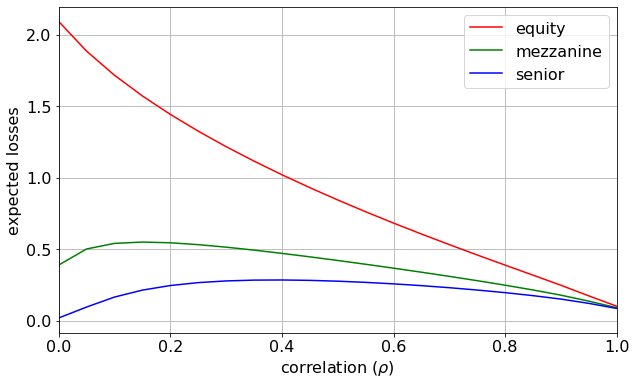
\includegraphics[width=0.7\textwidth]{figures/losses_vs_rho}
	\caption{Expected losses for each tranche as a function of the correlation parameter.}
	\label{fig:losses_rho}
\end{figure}

\begin{attention}
As noticed at the end of Section~\ref{standard-market-model}, in case the entities of the reference portfolio haven't the same default probabilities it is possible to determine Eq.~\ref{eq:def_prob_ex_cdo_1} numerically with an iterative procedure. The next snippet of code shows an example where ten names have different probabilities.

\pythoncodebox{code/credit_derivatives_8.py}
\begin{ioutput}
[0.5655235318063276, 0.350403844356834, 0.11955743831716371,
 0.0330669128164737, 0.007898678014359, 0.00081191731818153,
 5.350491409986e-05, 2.81423807427e-06, 1.2554827537575e-07,
 5.216612301099e-09, 2.08664492043e-10]
\end{ioutput}
\end{attention}

\subsection{Synthetic CDO Valuation}
Imagine a Synthetic CDO made of $N$ references in the portfolio, each one with the same notional amount (the total CDO notional is $F$).
When the $i^{th}$ reference defaults the portfolio incurs in a loss of $\frac{F}{N}(1-R)$ (the recovery rate is assumed to be the same for all names).

The tranche loss function $TL^{L,U}(l)$ for a given time $t$ is a function of the number of defaults $l$ occurred up to that time and is given by
\begin{equation}
TL_{t}^{L,U}=\mathrm{max}(\mathrm{min}(\cfrac{l}{N}\cdot F(1-R), U)-L, 0)
\end{equation}
where $\frac{l}{N}F(1-R)$ is the total portfolio loss, if it is greater than $U$ then the tranche loss is $U$, conversely if it is lower than $L$ there is no loss.

So for example suppose $L=3\%$ and $U=7\%$ and suppose also that the portfolio loss is $5\%$. Then the tranche loss is 2\% of the total portfolio notional (or 50\% of the tranche notional $=7\%-3\%=4\%$).

When an investor \emph{sells protection} on a tranche she is guaranteeing to reimburse any realized losses on the tranche to the \emph{protection buyer} (to better understand this concept it is useful to think of the protection as an \emph{insurance}). 
In return, the protection seller receives a premium at regular intervals (typically every three months) from the protection buyer.

\subsubsection{Premium Leg}
The premium leg payments are made at the end of each time interval and are proportional to the \textbf{remaining notional} in the tranche (this is another important difference with respect to CDS, where the contract ends as soon as a default occurs).

We can then write the NPV of the premium leg as

\begin{equation}
\mathrm{NPV}_{\mathrm{premium}}^{L,U}=S\sum^{n}_{i=1}D(d_i)\cfrac{(d_i - d_{i-1})}{360}\left(F(U-L)-\mathbb{E}[TL_{d-1}^{L,U}]\right)
\label{eq:cdo_npv_premium}
\end{equation}
where $n$ is the number of payment dates, $D(d_i)$ is the discount factor, $S$ is the annualized premium. The expected value represents the tranche loss at time $d_{i-1}$. Note that for simplicity we are ignoring that the default may take place at any time between each payment date.

\subsubsection{Default Leg}
The default leg represents the cash flows paid to the protection buyer upon losses occurring in the considered tranche. 

The NPV of the leg can be expressed as
\begin{equation}
\mathrm{NPV}_{\mathrm{default}}^{L,U}=\sum_{i=1}^{n}D(d_i)\left(\mathbb{E}[TL_{d_i}^{L,U}]-\mathbb{E}[TL_{d_{i-1}}^{L,U}]\right)
\label{eq:cdo_npv_default}
\end{equation}
where the argument in parenthesis is the expected losses between time $d_{i-1}$ up to $d_i$. 

From Equations~\ref{eq:cdo_npv_premium} and~\ref{eq:cdo_npv_default} it is clear that the key ingredient for the valuation of a CDO is the calculation of $\mathbb{E}[TL_{d_i}^{L,U}]$ which appears in both. Luckily using the Gaussian copula it is relatively easy to compute it. Indeed we know that 
\begin{equation}
TL_{t}^{L,U}=\mathrm{max}(\mathrm{min}(\frac{l}{N}\cdot F(1-R), U)-L, 0)
\label{eq:tl}
\end{equation}
where the only random variable is the number of defaults $l$. We also know that 
\begin{equation}
\mathbb{E}[TL_{t}^{L,U}] = \sum_{l=0}^{N}TL_{t}^{L,U}\cdot \int_{-\infty}^{\infty} P_{\mathrm{def}}(l(t|M)=j) \phi(M)dM
\label{eq:etl}
\end{equation}

And has we have already seen this calculation can be carried on without too much effort. The large popularity of the Gaussian copula just resides in this, it allows to compute very quickly very complicated contracts like CDOs which usually involve a large number of correlated names.

\subsection{CDO Fair Value}
The \emph{fair value} of a CDO tranche is that value of the premium $S^*$ for which the expected value of the premium leg equals the expected value of the default leg and for what we have seen depends on the expected value of the tranche loss function.

Given Equations~\ref{eq:cdo_npv_premium} and~\ref{eq:cdo_npv_default} it can be expressed as

\begin{equation}
S^* = \cfrac{\mathrm{NPV_{default}}^{L,U}}{\sum^{n}_{i=1}D(d_i)\cfrac{(d_i - d_{i-1})}{360}\left(F(U-L)-\mathbb{E}[TL_{d-1}^{L,U}]\right)}
\label{eq:cdo_fair_value}
\end{equation}

Equation~\ref{eq:cdo_fair_value} defines the CDO fair value, but can also be used to calibrate the implied correlation parameter from the market. This can be obtained by plugging into the equation the market premium value and solve for the correlation parameter $\rho$. It must be noted though that the derivation of the implied correlation coefficient is not that easy since the assumed model is so simple that may not fit well to real data. Indeed it is most likely that there will be different implied $\rho$s for each tranche (while the model assumes the same correlation everywhere).

As a last consideration we have to notice that all equations shown previously have been derived under the assumptions of the same notional and recovery rate for each entity in the portfolio. Nonetheless their generalization to different notional and recovery rate is pretty straightforward.
 
\begin{finmarkets}
Clearly this class too has to go into the \texttt{finmarkets} module. The following code implements a \texttt{CollDebtObligation} class.
\end{finmarkets}

\pythoncodenon{code/credit_derivatives_9.py}

Let's test the class with a CDO with 1 year maturity and a reference portfolio of 125 names. Each of them have the same default probabilities, defined through a credit curve (\texttt{cc}) and the correlation is set to 0.3. The risk free rate is flat at 5\%. The tenor has been chosen to 12 months mainly for performance reasons since the computation of the expected losses implies the integration in Equations~\ref{eq:tl} and \ref{eq:etl}, for each name, and for each payment date and this can be quite time consuming.
Tranches and premiums are defined as follows:
\begin{itemize}
	\item equity: [0.0, 0.03] (spread 0.15);
	\item mezzanine: [0.03, 0.06] (spread 0.07);
	\item senior: [0.06, 0.09] (spread 0.03);
	\item super-senior: [0.09, 1.0] (spread 0.01).
\end{itemize}

In the following example we are going to evaluate the fair value of each tranche of the contract.

\pythoncodenon{code/credit_derivatives_10.py}

\begin{ioutput}
Tranche 0 ([0.0, 0.03]): 0.15942
Tranche 1 ([0.03, 0.06]): 0.02505
Tranche 2 ([0.06, 0.09]): 0.00773
Tranche 3 ([0.09, 1.0]): 0.00017
\end{ioutput}

As expected the equity tranche has the higher fair value being the riskier, while the senior tranche is the safest hence the one with lower premium.

\section*{Exercises}
\begin{question}
Six companies have default probabilities of 1\%, 2\%, 5\%, 8\%, 11\% respectively for each of the next five years. Also the probabilities are correlated by $\rho=0.4$. Determine the 4th-to-default probabilities for each year when a Gaussian copula is used to model the defaults.
\end{question}

\cprotEnv\begin{solution}

The covariance matrix of the multivariate normal distribution has bee constructed by starting with a matrix whose values are all equal to $\rho$, then the diagonal elements have been zeroed.

\begin{ipython}
from scipy.stats import multivariate_normal, norm

p_default = [0, 0.01, 0.02, 0.05, 0.08, 0.11]
cov = np.ones(shape=(6, 6))*0.4
np.fill_diagonal(cov, 1.0)
mvnorm = multivariate_normal(mean=[0]*6, cov=cov)

n_to_default = 4
trials = 500000
result = [0., 0., 0., 0., 0., 0.]
x = mvnorm.rvs(size=trials)
sim_defaults = np.sort(norm.cdf(x))

for s in sim_defaults:
    for i in range(1, len(p_default)):
        if p_default[i-1] <= s[n_to_default-1] <= p_default[i]:
            result[i] += 1

print ("4th-to-default probabilities")
for i in range(len(p_default)):
    print (f"{i}: {result[i]/trials:.4f}")
\end{ipython}
\begin{ioutput}
4th-to-default probabilities
0: 0.0000
1: 0.0004
2: 0.0009
3: 0.0059
4: 0.0098
5: 0.0135
\end{ioutput}
\end{solution}

\begin{question}
Consider a 3-year 5th-to-default basket on ten reference entities in the situation where the copula correlation is 0.15 and the expected recovery rate, $R$, is $40\%$. The term structure of interest rates is assumed to be flat at 3\%. The default probabilities for the entities are 1\%, 3\% and 7\% respectively in one, two and three years from now.
Determine the breakeven rate and the NPV of the contract.
\end{question}

\cprotEnv\begin{solution}	
\begin{ipython}
from finmarkets import DiscountCurve, BasketDefaultSwaps
from datetime import date
from dateutil.relativedelta import relativedelta

n_cds = 10
rho = 0.15
l = 0.016
ndefaults = 5

obs_date = date.today()
start_date = obs_date
dates = [obs_date + relativedelta(years=i) for i in range(1, 4)]
dfs = [1/(1+0.03)**i for i in range(1, 4)]
dc = DiscountCurve(obs_date, dates, dfs)

basket = BasketDefaultSwaps(1e6, n_cds, l, rho, start_date, "3y", 0.01)
basket.credit_curve(obs_date, dates, ndefaults)
bkeven = basket.breakeven(dc)
print(f"breakeven rate: {bkeven:.5f}:")

new_basket = BasketDefaultSwaps(1e6, n_cds, l, rho, start_date, "3y", bkeven)
new_basket.credit_curve(obs_date, dates, ndefaults)
print(f"NPV: {new_basket.npv(dc):.0f}")
\end{ipython}
\begin{ioutput}
breakeven: 0.00017
NPV: -263
\end{ioutput}
\end{solution}

\begin{question}
Consider a Cash CDO with a maturity of 1 year, made of 125 bonds. Each bond pays a coupon of one unit after 1 year and it has not yet defaulted (the recovery rate $R$ is assumed 0). The CDO has three tranches: equity ([0, 3] defaults), mezzanine ([4, 6] defaults) and senior ([7, 125] defaults).
Draw the expected loss as a function of the correlation $\rho$ for the three tranches and show that the sum of the losses of each tranche is independent from $\rho$.
\end{question}

\cprotEnv\begin{solution}	
To solve this question we need to implement a function that evaluate through the one-factor copula model and the binomial distribution the probability of $l$ defaults.
Then we can compute the expected losses for each tranche and for various values of the correlation parameter $\rho$, saving into a list the results for later plotting.

\begin{ipython}
from scipy.stats import binom, norm
from scipy.integrate import quad
import numpy as np

N = 125
A = 1
R = 0
M = 1
q = 0.02
tranches = [[1,3],[4, 6],[7,125]]
def p(M, rho, lims):
    qM = max(1e-10, norm.cdf((norm.ppf(q)-np.sqrt(rho)*M)/(np.sqrt(1-rho))))
    pN = binom(N, qM)
    prob = (lims[1]-lims[0]+1) * (pN.cdf(N) - pN.cdf(lims[1]-1))
    for i in range(lims[0], lims[1]):
        prob += (i-lims[0]+1)*pN.pmf(i)
    return norm.pdf(M)*prob

res = [[],[],[]]
for i in range(len(tranches)):
    for rho in np.arange(0., 1.05, 0.1):
        if rho == 1.0:
            rho = 0.99
        v = quad(p, -np.inf, np.inf, args=(rho, tranches[i]))
        res[i].append(v[0])
\end{ipython}

\begin{figure}[htbp]
\begin{center}		
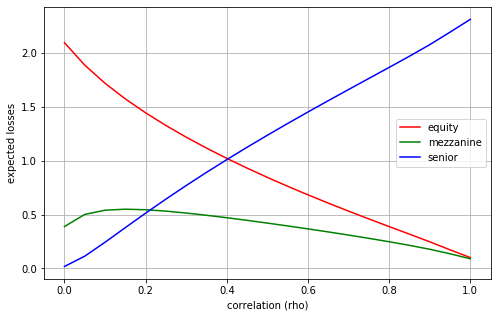
\includegraphics[width=0.7\linewidth]{figures/losses_vs_rho_2}
\end{center}
\end{figure}

To demonstrate that the total expected loss is independent from $\rho$ it is enough to print its values for a couple of different values of the correlation parameter. Since the expected loss of the tranches have been saved into lists the sum can be done among values of the lists with similar indices. 

\begin{ipython}
print (res[0][1] + res[1][1] + res[2][1])
print (res[0][5] + res[1][5] + res[2][5])
print (res[0][9] + res[1][9] + res[2][9])
\end{ipython}
\begin{ioutput}
2.500000000000001
2.5000000000019336
2.5000000062236856
\end{ioutput}
\end{solution}

\begin{question}
Determine the fair value of each tranche in a CDO with 1 year maturity and a reference portfolio of 125 names. Each of them have the same default probabilities, 1\%, and their correlation is set to 0.2. The tenor of the premium leg is 12 months. The risk free rate is flat at 5\%.
\begin{itemize}
	\item equity: [0.0, 0.03] (spread 0.20);
	\item mezzanine: [0.03, 0.06] (spread 0.01);
	\item senior: [0.06, 1.0] (spread 0.005).
\end{itemize}
How does these results change if the default probability raises to 5\% ? \\
How does these results change if instead there is an higher correlation (0.6) ?
\end{question}

\cprotEnv\begin{solution}

\begin{ipython}
from finmarkets import DiscountCurve, CreditCurve, CollDebtObligation
from datetime import date
from dateutil.relativedelta import relativedelta

pillar_dates = []
df = []
obs_date = date.today()
start_date = obs_date
dates = [obs_date + relativedelta(years=i) for i in range(1, 2)]
dfs = [1/(1 + 0.05)**i for i in range(1, 2)]
dc = DiscountCurve(obs_date, dates, dfs)

cc = CreditCurve(obs_date,
                 [obs_date + relativedelta(years=i) for i in range(1, 5)],
                 [0.99, 0.97, 0.95, 0.93])

nnames = 125
tranches = [[0.0, 0.03], [0.03, 0.06], [0.06, 0.09], [0.09, 1.0]]
spreads = [0.15, 0.07, 0.03, 0.01]

cdo = CollDebtObligation(100e6, nnames, tranches,
                         0.3, cc, start_date, spreads,
                         "1y", "12m")

for i in range(len(tranches)):
    print (f"Tranche {i} ({tranches[i]}): {cdo.fair_value(i, dc):.5f}")
\end{ipython}
\begin{ioutput}
Tranche 0 ([0.0, 0.03]): 0.17775
Tranche 1 ([0.03, 0.06]): 0.01570
Tranche 2 ([0.06, 1.0]): 0.00012
\end{ioutput}
With an higher default probability instead, the NPV of the default leg increases and so does the fair value.

\begin{ioutput}
Tranche 0 ([0.0, 0.03]): 0.59296
Tranche 1 ([0.03, 0.06]): 0.22714
Tranche 2 ([0.06, 1.0]): 0.00530
\end{ioutput}
Finally with a larger correlation the probability of multiple defaults increases leading to larger losses in safer tranches. So the fair value increases in mezzanine and senior tranches, but is lower in the equity where the probability of few defaults is reduced.

\begin{ioutput}
Tranche 0 ([0.0, 0.03]): 0.09899
Tranche 1 ([0.03, 0.06]): 0.03498
Tranche 2 ([0.06, 1.0]): 0.00192
\end{ioutput}
\end{solution}


\chapter{Risk Measures}
\label{var-and-credit-risk}

In quantitative finance arguably one of the most important challenge is the financial risk measurement and assessment.
The majority of the financial engineer’s task is connected to this field.
%Risk Measurement for a financial institution is very data intense and computational expensive process. Using the adequate, state of the art technologies is key to keep up with the speed of the financial market innovation, and to be able to meet the regulatory requirements.

There is a wide range of risk measures that spread through the Market: volatility ($\sigma$), Value at Risk (VaR), Expected Shortfall (ES) (Conditional Value at Risk), Average Drawdown, Maximum Drawdown, $\ldots$
In this Chapter we will concentrate specifically on two of them: VaR and ES.

\section{VaR and Expected Shortfall}
\label{value-at-risk}

\emph{Value-at-risk} (VaR) is defined as the loss level that will not be exceeded with a certain confidence level during a certain period of time.
\begin{equation}
\text{VaR}_{\alpha}(X) = -F^{-1}_X(\alpha)
\label{eq:var}
\end{equation}
Mathematically it is the loss corresponding to the $(100-X)^{th}$ percentile of the portfolio returns over the next $N$ days (e.g. in Figure~\ref{fig:var_loss} the graphical representation of the VaR, with $N=1$ and $X=95$, is shown; in the example a normal distribution for the changes in value is assumed). By definition it is a function of two parameters: the time horizon (i.e. $N$ days usually set to 1) and the confidence level (usually 95\%). 

\begin{figure}[htb]
\centering
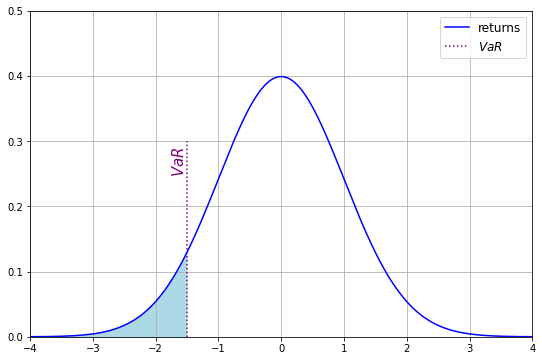
\includegraphics[width=0.6\linewidth]{figures/95_var}
\caption{Example of $VaR$ on the distribution of changes in value.}
\label{fig:var_loss}
\end{figure}

For example, if a bank's 10-day 95\% VaR is 3 million USD, there is considered to be only a 5\% chance that losses will exceed 3 million USD in 10 days.

One problem with VaR is that, when used in an attempt to limit the risks taken by a trader, it can lead to undesirable results. Suppose a bank tells a trader that the one-day 95\% VaR of the trader's portfolio must be kept less than 10 million USD. There is a danger that the trader will construct a portfolio where there is a 95\% chance that the daily loss is less than 10 million USD and a 5\% chance that it is 500 million USD. The trader is satisfying the risk limits imposed by the bank, but is clearly taking unacceptable risks. 

The problem is summarized in Figure~\ref{fig:var_vs_badvar}. It shows the probability distribution for the gain or loss on a portfolio over a specified period of time. Both portfolios have the same VaR. However, the portfolio on the right is much riskier than the portfolio on the left because potential losses are much larger. 

\begin{figure}[htb]
\centering
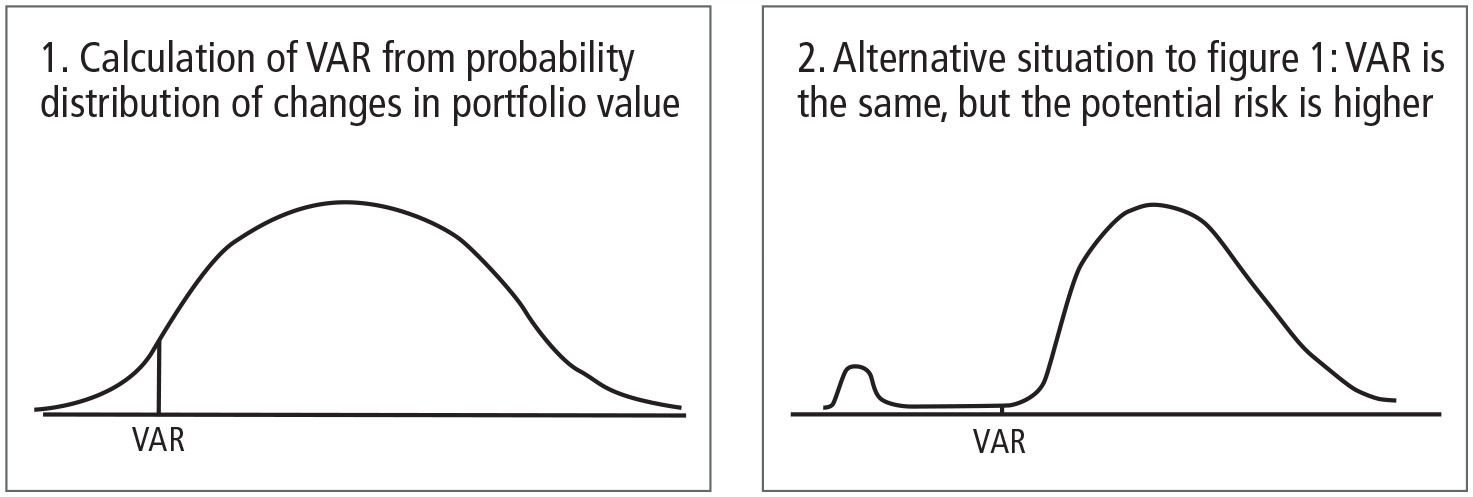
\includegraphics[width=0.8\linewidth]{figures/var_badvar}
\caption{Probability distribution for the gain or loss on a portfolio over a specified period of time. Both portfolios have the same VaR. However, the portfolio on the right is much riskier than the portfolio on the left because potential losses are much larger.}
\label{fig:var_vs_badvar}
\end{figure}

Furthermore VaR hasn't the \textit{sub-additivity property}. So given a portfolio with two assets it is \textbf{not} guaranteed that
\begin{equation*}
\text{VaR}_A +  \text{VaR}_B \geq  \text{VaR}(A+B)	
\end{equation*}

A measure that produces better incentives for traders than VaR is \emph{expected shortfall} (ES). This can be also referred to as conditional VaR. Where VaR asks the question 'how bad can things get?', expected shortfall asks 'if things do get bad, what is our expected loss?'. It is the expected loss during an N-day period, conditional that the loss is greater than the $X^{th}$ percentile of the loss distribution
\begin{equation}
\text{ES}_{\alpha}(X) = \frac{1}{\alpha}\int_0^\alpha \text{VaR}_p(X) dp
\label{eq:es}
\end{equation}

For example, with $X = 99$ and $N = 10$, the expected shortfall is the average amount that is lost over a 10-day period, assuming that the loss is greater than the $99^{th}$ percentile of the loss distribution.  Clearly, the expected shortfall is much higher in Figure~\ref{fig:var_vs_badvar} (right) than (left). 

Expected shortfall is the negative of the expected value of the tail beyond the VaR, hence it is always a equal to or larger than the corresponding VaR, see Figure~\ref{fig:es_loss}.

\begin{figure}[htb]
\centering
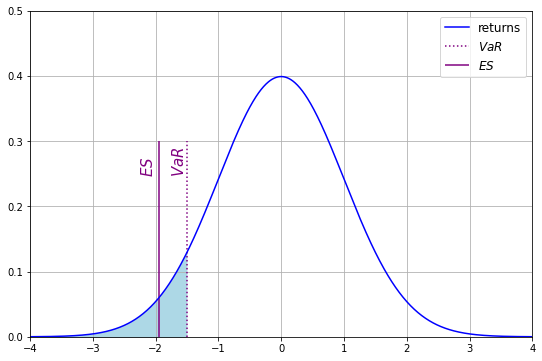
\includegraphics[width=0.6\linewidth]{figures/es}
\caption{Example of 95\% VaR on the distribution of changes in value.}
\label{fig:es_loss}
\end{figure}

Regulators make extensive use of VaR and its importance as a risk measure is therefore unlikely to diminish. However, expected shortfall has a number of advantages over VaR, and this has led many financial institutions to use it as a risk measure internally. 
Contrary to VaR, Expected Shortfall follows the sub-additivity property.

%For details about how to perform the integral in Eq.~\ref{eq:es} refer to Section~\ref{sec:integration}.

\section{How to Compute Risk Measures}
\label{how-to-estimate-the-var}

Throughout this Section the historical series of following tickers AAPL, CSCO, GOOG, INTC, NVDA are used to create an equally weighted reference portfolio. The dataset with their historical series between January 2023 and September 2024 is available in \href{https://raw.githubusercontent.com/matteosan1/finance_course/develop/input_files/historical_data.csv}{historical\_data.csv}.

\subsection{Parametric VaR, ES}

The historical performance of the portfolio can be determined by the series of the constituents. It has been checked that the return distributions are all approximately Gaussian, see Fig.~\ref{fig:asset_return_distro}.

\begin{figure}[htb]
	\centering
	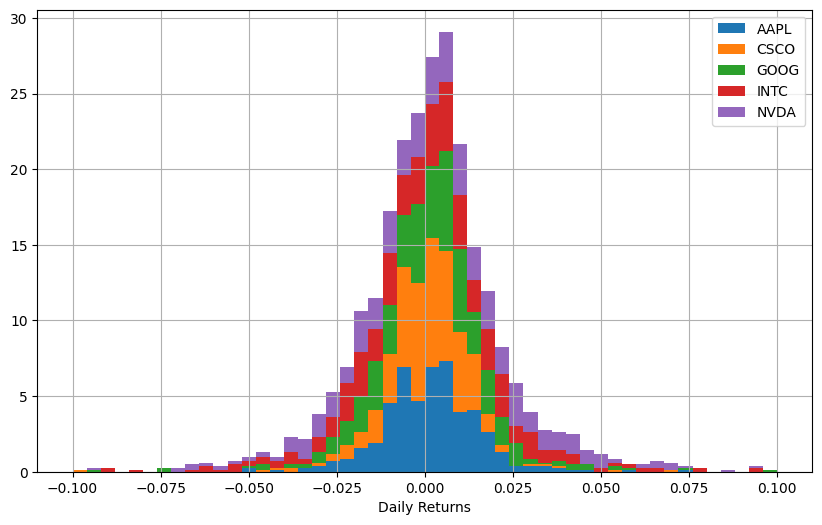
\includegraphics[width=0.6\textwidth]{figures/asset_return_distro}
	\caption{Stacked histogram showing the return distributions of the asset involved in the studied portfolio. The overall distribution is indeed a scaled version of the historical performance histogram of the portfolio. All the returns are approximately distributed as a Gaussian.}
	\label{fig:asset_return_distro}
\end{figure}

Below are reported the resulting VaR and ES using the normal and the t-student models, computed passing in turn the two fitted models.

\pythoncodenon{code/var_var_continuous.py}
\begin{ioutput}
Gaussian
1d-95% VaR: 0.022
1d-95% ES: 0.02801

t-student
1d-95% VaR: 0.02115
1d-95% ES: 0.029971
\end{ioutput}

%\subsection{Historical Simulation}
%\label{historical-simulation}
%
%When it is not obvious which distribution the portfolio returns belong to, it is possible to avoid any assumption by random sampling on the historical returns directly. The obvious advantage of this technique is that no parameter estimation is required, the drawback being that such kind of simulation heavily relies on the assumption that past behaviors are indicative of what might happen in the future. That's why it is important that out historical series was as large as possible otherwise our results will be affected by lack of statistics. 
%
%\begin{finmarkets}
%The \texttt{finmarkets} module has also two functions to compute VaR and ES for the discrete case. They rely on the sampling from the original historical series which has been implemented in a separated utility function. The fastest way to generate random sample of historical returns is to assign an integer for each observation, and, using a random sampling algorithm, we can generate the set of simulated returns. Then the risk measures are calculated as percentiles of the the generated distributions.
%\end{finmarkets}
%
%\pythoncodenon{code/var_var_historical.py}
%\begin{ioutput}
%1d-95% VaR (discrete): 0.0201
%1d-95% ES (discrete): 0.0319
%\end{ioutput}
%
%Figure~\ref{fig:historical_var} shows the results. Notice again that the generated return distributions suffers from the same limitation of the original historical series (e.g. missing data in specific regions).
%
%\begin{figure}[htb]
%\centering
%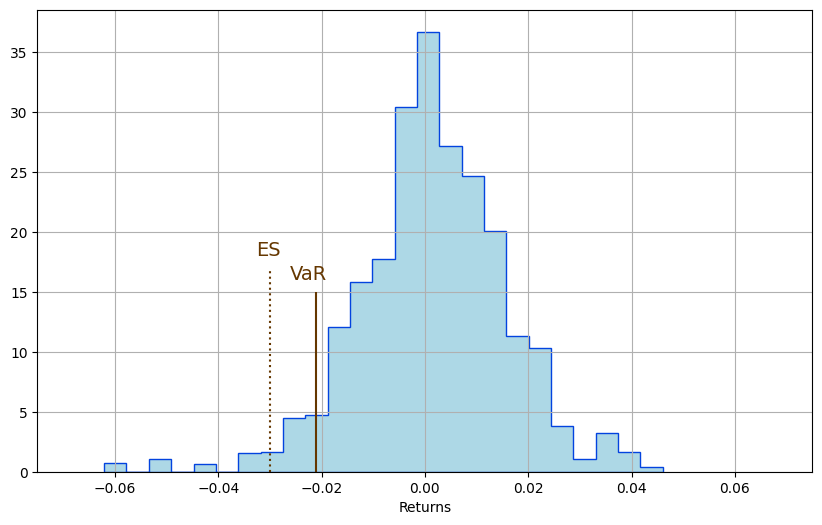
\includegraphics[width=0.6\textwidth]{figures/historical_var}
%\caption{Distribution of the return random sampling. The corresponding $VaR$ and $ES$ are also shown.}
%\label{fig:historical_var}
%\end{figure}

\section{Credit VaR}
\label{credit-var-cr-var}

\emph{Credit VaR} is defined in the usual way other risk measures are (i.e. as percentile of a loss distribution). In this case we are concerned with the default risk associated to one or multiple counter-parties in a specific portfolio instead with to the market risk.

To derive the loss distribution we need to consider the exposure $\text{EE}(\tau)$ defined as the sum of the discounted cash flows at the default date $\tau$. The corresponding loss is then given by

\begin{equation}
L_{\tau} = (1 - R) \cdot \textrm{EE}(\tau)
\end{equation}
where $L$ is non-zero only in scenarios of early counter-party default. 

Given the above definitions we can express the Credit VaR as the (100-X)-quantile of $L_{\tau}$. With respect to the Value at Risk, the time horizon is usually set to one year and the percentile to $99.9^{th}$, so it returns the loss that is exceeded only in 1 case out of 1000. 

Note that in this case quantile has to be computed on the "positive" tail of the loss distribution, because $L$ represents the loss value (i.e. it is a positive quantity).

%Credit VaR is actually either the difference of the percentile from the mean, or the percentile itself. There is more than one possible definition, anyway we  will use the latter.

\subsection{Credit VaR and MC Simulation}
\label{sec:credit-var-sim}

Credit VaR can be calculated through a simulation of the evolution of a portfolio up to the risk horizon; the simulation must of course include possible defaults of the counter-parties. In each experiment the portfolio is priced obtaining a number of scenarios to draw the loss distribution.

Consider a portfolio of 3 swaps all with a 5y maturity and a fixed rate respectively of (3\%, 2.85\% and 3.3\%) on nominals of (1M, 2M and 1.5M).

The recovery rate in case of default is 40\% and the risk free rate is flat at 2.5\% while the EURIBOR rate is assumed to be flat at 3.5\%.

\pythoncode{code/var_cvar.py}
\begin{ioutput}
NPV portfolio: 97,617.16 EUR
Portfolio Credit VaR (at 95% c.l.) 50,203.11 EUR
\end{ioutput}
Results are also reported in Fig.~\ref{fig:credit_var_uncorr}.

\begin{figure}[htb]
	\centering
	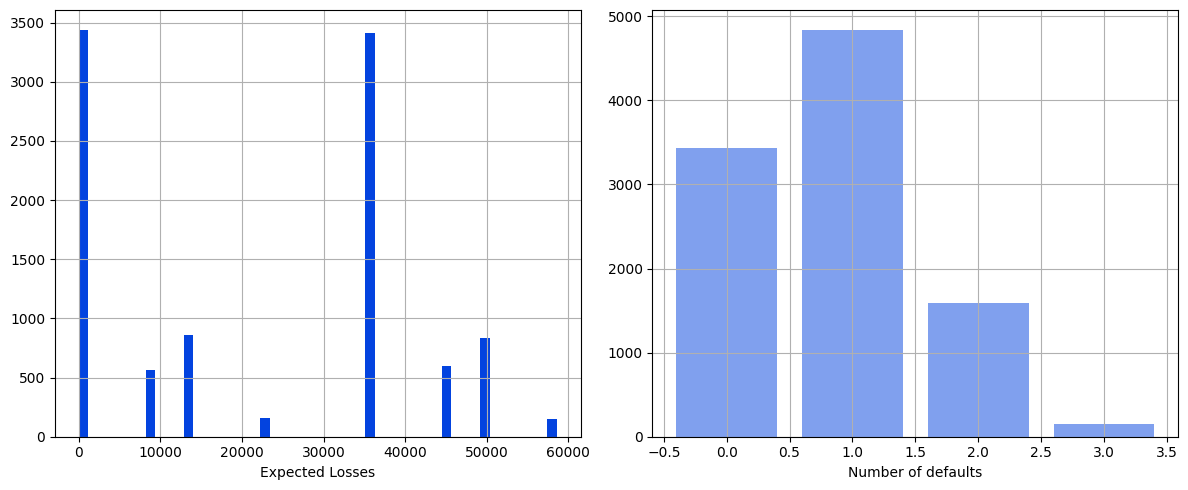
\includegraphics[width=0.9\textwidth]{figures/credit_var_uncorr}
	\caption{Distribution of losses (left) and number of defaults per scenario (right).}
	\label{fig:credit_var_uncorr}
\end{figure}

If these swaps belong to counterparties subject to systematic market risk, assuming independent defaults will underestimate tail risk.

So repeat the exercise modeling default clustering through a Gaussian Copula with:
\begin{itemize}
	\item correlation structure $\rho=0.9999995$ and $P_{\text{def}} = [0.2, 0.2, 0.2]$
	\item correlation structure $\rho=0.9999995$ and $P_{\text{def}} = [0.2, 0.5, 0.15]$
\end{itemize}

\begin{ipythonnon}
from scipy.stats import binom

from copulas import Copula

np.random.seed(42)
n_sims = 10000
PD = np.array([0.2, 0.2, 0.2])
#PD = np.array([0.2, 0.5, 0.15])
R = 0.4
LGD = 1 - R

rho = 0.9999995
correlation = np.full((3, 3), rho)
np.fill_diagonal(correlation, 1.0)

copula = Copula(3, "gauss", {'corr':correlation})
...
\end{ipythonnon}
A comparison of the two cases is reported in Fig.~\ref{fig:credit_var_corr}. Compared to the uncorrelated case (blu bars) the number of simulations with 0 or a single default are reduced in both scenarios. Contrary there is substantial increase in the number of three defaults events.

Comparing the two correlated results emerges a clear threshold effect: when the $\Pdef$s are all equal there are not 1 or 2 default events since the portfolio is equivalent to a single asset. On the other hand, when the assets have different default probabilities, despite the perfect correlation, there are also intermediate scenarios.

\begin{figure}[htb]
	\centering
	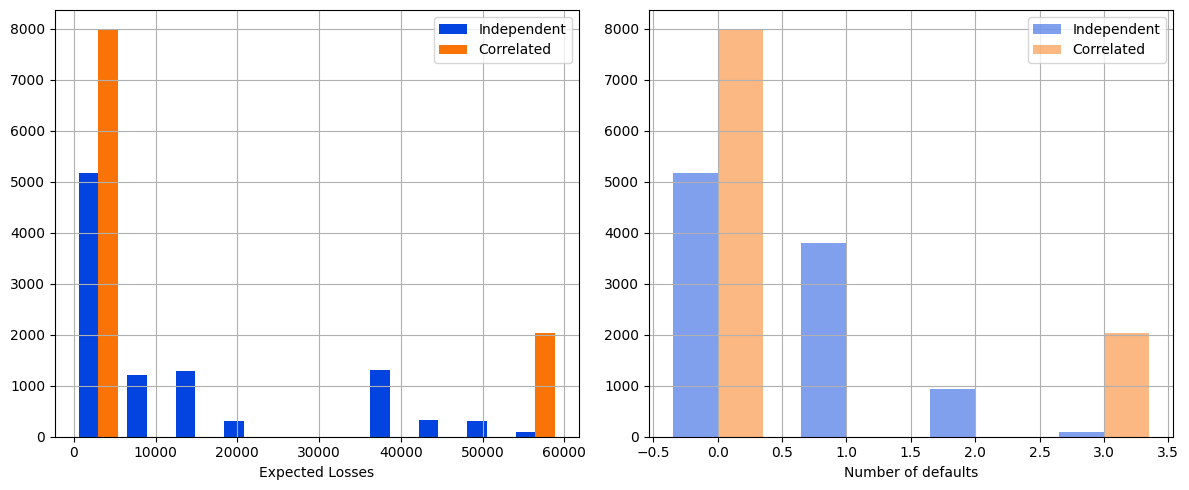
\includegraphics[width=0.9\textwidth]{figures/credit_var_corr_v1}\\
	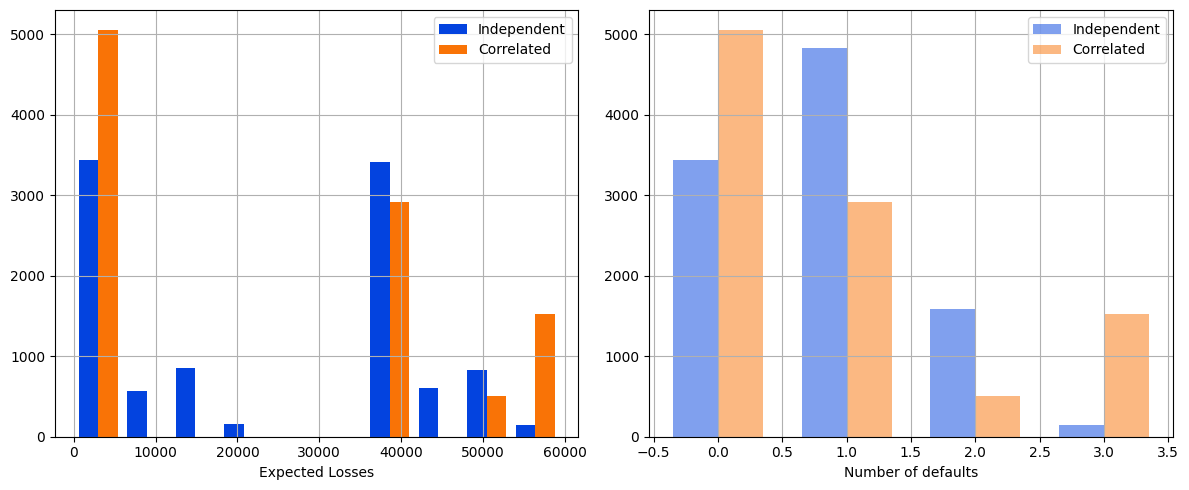
\includegraphics[width=0.9\textwidth]{figures/credit_var_corr_v2}
	\caption{Distribution of losses (left) and number of defaults per scenario (right) for the two cases described in the text: $PD = [0.2, 0.2, 0.2]$ (upper) and $ PD=[0.2, 0.5, 0.15]$ (bottom).}
	\label{fig:credit_var_corr}
\end{figure}


%Consider, for example, a portfolio of five fixed coupon bonds (0.1) each one with the same default probability (a Poisson process with $\lambda=0.5$) and the same face value (100 EUR). The recovery rate in case of default is $R=40\%$ and the discount curve is the one stored in \href{https://github.com/matteosan1/finance_course/raw/master/input_files/discount_factors_2022-10-05.xlsx}{discount\_curve.xlsx}.
%
%In order to better simulate the evolution of the portfolio a helper function \texttt{Bond} is implemented: it is just able to compute the bond NPV at a given date. Also a set of default times has been calculated using \texttt{PoissonProcess} distribution.
%Notice that in this simple example there is no need to run multiple scenarios since any market parameters of the portfolio is changing and no evolution is required (e.g. interest rate is fixed).
% 
%\begin{ipython}
%from finmarkets import generate_dates, maturity_from_str
%
%class Bond:
%    def __init__(self, face_value, start_date, tenor, maturity):
%        self.FV = face_value
%        self.tau = maturity_from_str(tenor, "y")
%        self.payment_dates = generate_dates(start_date, maturity, tenor)
%
%    def npv(self, d, dc, fc):
%        val = 0
%        for i in range(1, len(self.payment_dates)):
%            C = fc.forward_rate(self.payment_dates[i-1], self.payment_dates[i])
%            if self.payment_dates[i-1] <= d < self.payment_dates[i]:
%                rateo = (self.payment_dates[i] - d).days/
%                (self.payment_dates[i] - self.payment_dates[i-1]).days
%                val += C*rateo*self.tau*dc.df(d)
%            elif self.payment_dates[i] > d:
%                val += C*self.tau*dc.df(self.payment_dates[i])
%                val += dc.df(self.payment_dates[-1])
%        return self.FV*val
%\end{ipython}
%\begin{ipython}
%import pandas as pd
%import numpy as np
%from datetime import date
%from dateutil.relativedelta import relativedelta
%from finmarkets import DiscountCurve, CreditCurve, ForwardRateCurve
%from finmarkets import PoissonProcess, generate_dates
%    
%start_date = date.today()
%df = pd.read_excel("discount_curve.xlsx")
%pillars = [start_date + relativedelta(months=i) for i in df['months']]
%dc = DiscountCurve(pillars, df['dfs'])
%
%bonds = []
%maturity = "2y"
%
%fc_dates = generate_dates(start_date, maturity, "1y")
%rates = [0.1 for _ in range(len(fc_dates))]
%fc = ForwardRateCurve(start_date, fc_dates, rates)
%
%for i in range(len(coupons)):
%    bonds.append(Bond(100, start_date, coupons[i], 1, maturity))
%
%np.random.seed(1)
%N = 100000
%R = 0.4
%horizon = 1
%
%Q = PoissonProcess(l=0.5)
%cov = np.ones(shape=(len(bonds), len(bonds)))*rho
%np.fill_diagonal(cov, 1)
%g = GaussianCopula(len(bonds), cov)
%taus = Q.ppf(g.sample(N))
%
%L = []
%for n in range(N):
%    EE = 0
%    for i, b in enumerate(bonds):
%        if taus[n, i] <= horizon:
%            d = start_date + relativedelta(days=365*taus[n, i])
%            EE += b.npv(dc, d)
%    if EE != 0:
%        L.append((1-R)*EE)
%  
%print (np.percentile(L, [95.0]))
%\end{ipython}
%\begin{ioutput}
%338.0718924883006
%\end{ioutput}
%\noindent
%Figure~\ref{fig:credit_var} shows the loss distribution of the portfolio. Each peak corresponds to scenarios where there is an increasing number of defaults and is located roughly at multiple of 60 since each bond value is around 100 which gives a loss of that size (i.e. $1-R$ with $R\simeq$40\%). 
%
%\begin{figure}[htb]
%\centering
%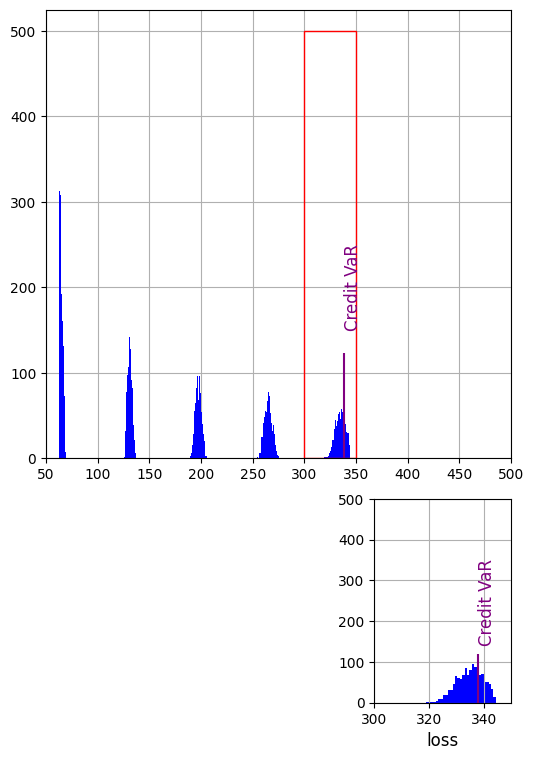
\includegraphics[width=0.5\textwidth]{figures/credit_var}
%\caption{Distribution of losses in a portfolio made of five fixed coupon bonds. In the zoom the tail of the plot is shown to highlight the Credit VaR value.}
%\label{fig:credit_var}
%\end{figure}

%\subsection{Credit VaR and One Factor Copula Model}
%Consider a portfolio made of similar assets. As an approximation assume that the probability of default is the same for each counter-party and that the correlation between each pair is the same and equal to $\rho$. Under these assumption the One Factor Copula model can be used to describe the default correlations (see Eq.~\ref{eq:gaussian_one_factor_copula})
%
%\begin{equation}
%\mathcal{Q}_M(T) = \Phi\Big(\cfrac{\Phi^{-1}[Q(T)]-M\sqrt{\rho}}{\sqrt{1-\rho}}\Big)
%\label{eq:conditional_default_prob}
%\end{equation}
%where $\Phi$ is the cumulative distribution function of the standard normal.
%
%Since there are $n$ counter-parties with the same default probability $\mathcal{Q}_M(T)$ the percentage of defaults at time $T$ is $\mathcal{Q}_M$ itself ($\textrm{\% of defaults} = \textrm{n\_defaults}/n = n\cdot \mathcal{Q}_M/n$). Hence Eq.~\ref{eq:conditional_default_prob} gives the percentage of defaults by time $T$ given $M$. 
%
%Since $M$ is distributed according to a standard Gaussian we can be $X\%$ certain that its value will be \emph{greater} than $\hat{m} = \Phi^{-1}(1-X)=-\Phi^{-1}(X)$, where the equality holds due to the symmetry of the Gaussian distribution (see Figure~\ref{fig:certain_for_X}).
%
%\begin{figure}[htb]
%\centering
%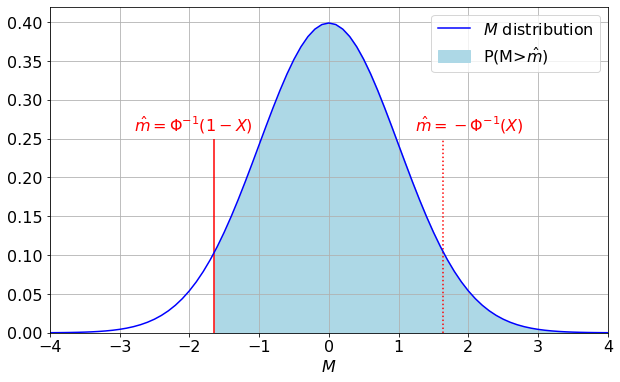
\includegraphics[width=0.7\textwidth]{figures/certain_for_X}
%\caption{$X\%$ probability to get an higher value a threshold for a normally distributed random variable.}
%\label{fig:certain_for_X}
%\end{figure} 
%
%Once the time $T$ has been chosen the only random variable appearing in the conditional default probability expression of Eq.~\ref{eq:conditional_default_prob} is $M$, therefore we can be $X\%$ certain that the percentage of defaults over $T$ years on a large portfolio will be \textbf{less} than $V(X,T)$ where
%
%\begin{equation*}
%V(X,T)= \Phi\Big(\cfrac{\Phi^{-1}[Q(T)]-\hat{m}\sqrt{\rho}}{\sqrt{1-\rho}}\Big) = \Phi\Big(\cfrac{\Phi^{-1}[Q(T)]+\Phi^{-1}(X)\sqrt{\rho}}{\sqrt{1-\rho}}\Big)
%\end{equation*}
%
%When the confidence level is $X\%$ and the time horizon is $T$, a rough estimate of the Credit VaR is therefore $P(1-R)V(X,T)$, where $P$ is the portfolio size and $R$ is the recovery rate.
%
%Suppose that a bank has a total of \euro{100} million of retail exposures. The 1-year probability of default averages to 2\% and the recovery rate averages to 60\%. The copula correlation parameter is estimated as 0.1.
%The 1-year 99.9\% Credit VaR is therefore \euro{5.13} million.

\subsection{CreditMetrics}
Another popular approach to estimate Credit VaR is \emph{CreditMetrics}. It involves computing a probability distribution of credit losses by carrying out Monte Carlo simulations of the counter-party credit rating changes.

Imagine we would like to determine the probability distribution of losses over 1-year period. On each simulation, we are going to determine the credit rating of each counter-party using the estimated probability of migration between one rate to another (or to default). Since the portfolio value depends on its asset ratings we can determine the eventual losses. 

As an example consider Table~\ref{tab:credit_ratings} which shows the percentage probability of a bond moving from one category to another during a 1-year period.

\begin{table}[htb]
\centering
\begin{tabular}{|l|c|c|c|c|c|c|c|c|}
\hline
Initial rating & AAA & AA & A & BBB & BB & B & CCC & default \\
\hline
\hline
AAA & 90.81 & 8.33 & 0.68 & 0.06 & 0.08 & 0.02 & 0.01& 0.01 \\ 
\hline
AA & 0.70 & 90.65 & 7.79 & 0.64 & 0.06 & 0.13 & 0.02 & 0.01 \\ 
\hline
A & 0.09 & 2.27 & 91.05 & 5.52 & 0.74 & 0.26 & 0.01 & 0.06 \\ 
\hline
BBB & 0.02 & 0.33 & 5.95 & 85.93 & 5.30 & 1.17 & 1.12 & 0.18 \\
\hline
BB & 0.03 & 0.14 & 0.67 & 7.73 & 80.53 & 8.84 & 1.00 & 1.06 \\
\hline
B & 0.01 & 0.11 & 0.24 & 0.43 & 6.48 & 83.46 & 4.07 & 5.20 \\
\hline
CCC & 0.21 & 0 & 0.22 & 1.30 & 2.38 & 11.24 & 64.86 & 19.79 \\		
\hline
\end{tabular}
\caption{Example of table with transition probabilities (in percent) between different credit rating categories.}
\label{tab:credit_ratings}
\end{table}

For a correct implementation of this technique credit rate changes cannot be assumed independent, hence a copula approach could be implemented.
Another possibility is the application of Markov chains~\ref{sec:markov_chain}, with the transition matrix which can be deduced by the numbers in Table~\ref{tab:credit_ratings}.

In fact the main difficulty in this application is precisely the determination of the transition matrix. These probabilities could be estimated by analyzing historical data from credit rating agencies, such as Standard\&Poor, Moody's and Fitch. But this could lead to unreliable numbers in case the future does not develop as smoothly as the past. It can therefore be more reliable to base the estimates on a combination of empirical data and more subjective, qualitative data such as opinions from experts. This is because the market view is a mixture of beliefs determined by both historical ratings and a more extreme view of the ratings. 

Another problem with deciding the transition matrix is that maybe it is not appropriate to use a \emph{homogeneous} Markov chain to model credit risk over time. In this kind of chain the transition matrix is considered constant, but it is clearly a crude approximation of reality which doesn't capture the time-varying behavior of the default risk. A non-homogeneous model could be more realistic, but on the other hand more complicated to use. 

\section{Credit Valuation Adjustment}
\label{credit-valuation-adjustment}

Suppose you have a portfolio of derivatives. If a counter-party defaults and the present value of the portfolio at default is positive to the surviving party (you), then the actual gain is only given by the recovery fraction of the value. If however the present value is negative to you, you have to pay it in full to the liquidators of the defaulted entity.

This behavior creates an asymmetry which can be corrected by changing the definition of the deal value as the value without counter-party risk minus a positive adjustment, called \emph{Credit Valuation Adjustment} (CVA).

The CVA can be expressed in the following way:

\begin{equation}
\text{CVA} = (1-R) \int_0^T D(t) \cdot \textrm{EE}(t)\cdot dQ(t)
\label{eq:cva}
\end{equation}
where $T$ is the latest maturity in the portfolio, $D$ is the discount factor, EE is the expected exposure or $\mathbb{E}[\max(0, NPV_{portfolio})]$, and $dQ$ is the probability of default between $t$ and $t+dt$.

For an easier computation it is natural to discretize the above integral and use a time grid going from 0 to the portfolio maturity:

\begin{equation}
\text{CVA} = (1-R) \sum_i^n D(t_i) \cdot \mathrm{EE}(t_i)\cdot Q(t_{i-1}, t_i)
\label{eq:cva_discrete}
\end{equation}

It is important to note the difference between Credit VaR and CVA. While the former measures the risk of losses faced due to the possible default of some counter-party, the latter measures the pricing component of this risk, i.e. the price adjustment of a contract due to this risk.

\subsection{Debit Valuation Adjustment}

The adjustment seen from the point of view of our counter-party is positive, and is called Debit Valuation Adjustment, DVA. It is positive because the early default of the client itself would imply a discount on its payment obligations, and this means a gain. So the client marks an adjustment over the risk free price by adding the positive amount called DVA. 

When both parties have non-null default probabilities, they consistently include both defaults into the valuation. So they will mark a positive CVA to be subtracted and a positive DVA to be added to the default risk free price of the deal. The CVA of one party will be the DVA of the other one and vice versa.

\begin{equation*}
\textrm{price}=\textrm{default risk free price + DVA - CVA}
\end{equation*}
Now, since
\begin{equation*}
\begin{gathered}
\textrm{default risk free price(A)} = - \textrm{default risk free price(A)} \\
\textrm{DVA(A)} = \textrm{CVA(B)} \\
\textrm{DVA(B)} = \textrm{CVA(A)} 
\end{gathered}
\end{equation*}
we get that eventually
\begin{equation*}
\textrm{price(A)} = -\textrm{price(B)}
\end{equation*}
so that both parties agree on the price, or, we could say, there is money conservation.

\subsection{CVA Computation}

The computation of the CVA is carried on with Monte Carlo simulation. 
First calculate the portfolio value at each time point for each MC scenario. Then estimate the CVA using either Eq.~\ref{eq:cva} or its discrete form in Eq.~\ref{eq:cva_discrete}. Finally average the CVA of all the scenarios to get its value.

\subsubsection{Example}
The issuer of a 1-years ZCB (Company A) has a default probability over the bond lifetime that can be modeled with a Poissonian Process with constant hazard rate. Compute the CVA contribution the ZCB price assuming that the interest rate term structure is simulated according to the Vasicek Model.

Inputs:
\begin{itemize}
\item Vasicek Model parameters: $a=0.3$, $b=0.05$ and $\sigma=0.03$;
\item current interest rate is $r_0 =0.03$;
\item recovery rate $R = 40\%$;
\item Company A hazard rate: $\lambda = 0.05$.
\end{itemize}

CVA can be estimated with Monte Carlo simulation through the following formula:

$$
CVA = \frac{1}{N}\sum_{n=0}^N \left[\sum_i \underbrace{LGD}_{\text{loss given default}} \cdot \underbrace{D(t_i)\cdot EE(t_i)}_{\text{ZCB value at time }t_i}\cdot \underbrace{PD(t_{i-1}, t_i)}_{\text{default probability in }[t_{i-1},t_i]}\right]
$$
Let's consider each term of the expression and how we can work them out.
\subsubsection{Loss Given default}
This is the easiest part, we have been given the recovery rate (40\%) so $LGD = 1 - R = 0.6$.

\subsubsection{ZCB Value at $t_i$}
Since for each simulation we are looping \textbf{daily} between $t_0$ (today) to $T$ (bond maturity = 1 year) we need to compute:
$$
D(t_i)\cdot EE(t_i) = e^{-r_i\cdot t_i} = P(t_i, T)
$$
The exercise asks to model the interest rates term structure using the Vasicek Model with parameters ($a=0.3$, $b=0.05$, $\sigma=0.03$ and $r_0 =0.03$).
Given its characteristics the model provides us with a simple way to directly compute the ZCB price as
$$
P(t_i, T) = A e^{B\cdot t_i}
$$
So we first simulate $N=10000$ paths for the short rate evolution then we can apply the simple formula for the ZCB price (we are considering unit nominal value).

\subsubsection{Default Probability between $[t_{i-1}, t_i]$}

We know that Company A, our counterparty, has an estimated constant hazard rate $\lambda = 0.05$. As we have seen we can model the default probability using a Poisson process
$$
P_{\text{def}} = 1 - e^{-\lambda \cdot (t_i-t_0)}
$$

The entire code is reported below:

\pythoncodenon{code/var_cva.py}

\begin{ioutput}
Bond price without adjustment: 0.9679
CVA: 0.029
Price: 0.9392
CVA/Rf-Price: 0.030
\end{ioutput}

\emph{Expressing the CVA as a fraction of the notional can be a useful way to compare the credit risk of different contracts.}
This percentage represents the expected loss due to credit risk as a proportion of the contract's nominal value.
%Figure~\ref{fig:cva_distribution} reports the evolution of the exposure in the swap as time flows.

%\begin{figure}[htb]
%	\centering
% 	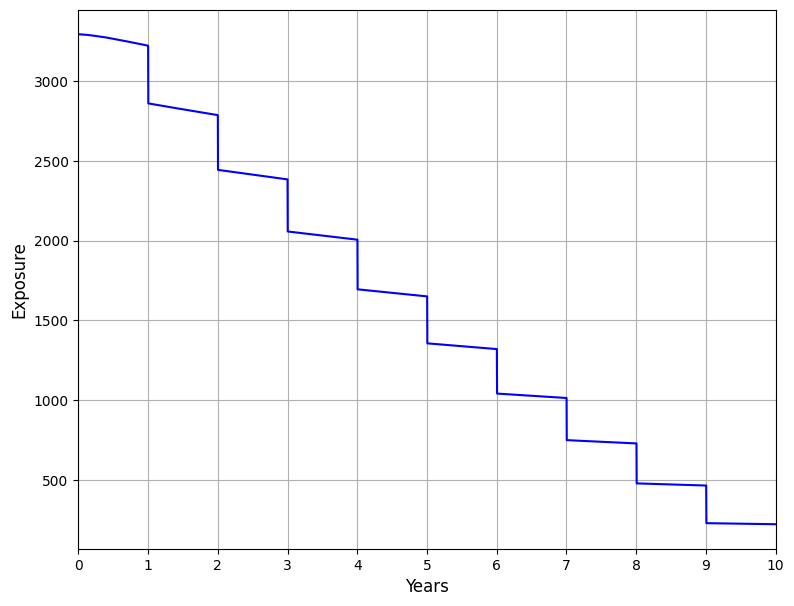
\includegraphics[width=0.65\textwidth]{figures/cva_exposure}
% 	\caption{Swap exposure as a function of time.}
% 	\label{fig:cva_exposure}
%\end{figure} 

\section*{Exercises}
\begin{question}
Given the historical series of three stock prices in the file \href{https://raw.githubusercontent.com/matteosan1/finance_course/master/input_files/historical.csv}{historical.csv} compute the 1-day 95\% VaR and the corresponding Expected shortfall for a portfolio consisting of 40 FOX shares, 35 ABC shares and 25 CBS shares. 

\noindent\textbf{Hint:} when simulating the historical scenarios take care of possible NaN values in the series.
\end{question}

\cprotEnv\begin{solution}
\begin{ipython}
import pandas as pd
import numpy as np

df = pd.read_csv("historical.csv", index_col='date')
w = np.array([0.4, 0.25, 0.35])

df['P'] = df[['FOX', 'CBS', 'ABC']].dot(w)
df = df.pct_change()
df.dropna(inplace=True)
print (df.head())
\end{ipython}
\begin{ioutput}
                 FOX       CBS       ABC         P
date                                              
2018-03-26  0.013858 -0.012607  0.011189  0.006395
2018-03-23 -0.030891 -0.046818 -0.010830 -0.024072
2018-03-22  0.020592  0.020093  0.011543  0.015722
2018-03-21  0.003317  0.012137  0.052941  0.031266
2018-03-20 -0.003306 -0.011991 -0.003464 -0.005276
\end{ioutput}
\begin{ipython}
from numpy.random import seed, choice
from numpy import percentile
from finmarkets import var_discrete, es_discrete
 
var = var_discrete(df, 0.95, 'P')
es = es_discrete(df, 0.95, 'P')

print ("VaR: {:.4f}".format(var))
print ("ES: {:.4f}".format(es))
\end{ipython}
\begin{ioutput}
VaR: 0.0173
ES: 0.0232
\end{ioutput}
\begin{figure}[htbp]
\centering
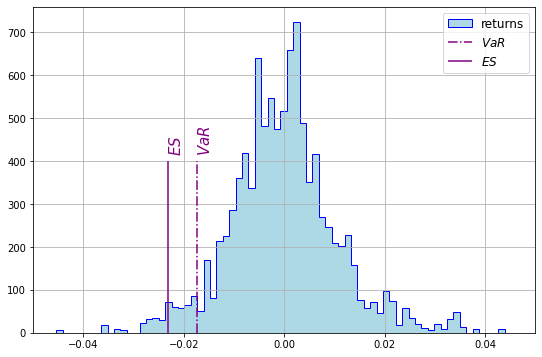
\includegraphics[width=0.7\linewidth]{figures/hist_var_ex}
\end{figure}
\end{solution}

\begin{question}
You have a 3-years call with strike 110 EUR. The underlying initial price is 105 EUR with a volatility of 0.15. The risk-free rate is 0.03 flat.
Compute the CVA of the contract assuming a recovery rate of 40\% and default probabilities for the underlying of 10\%, 20\% and 30\% for first, second and third year respectively.
\end{question}

\cprotEnv\begin{solution}
Below are shown ten realizations of the underlying price.

\begin{figure}[htbp]
\centering
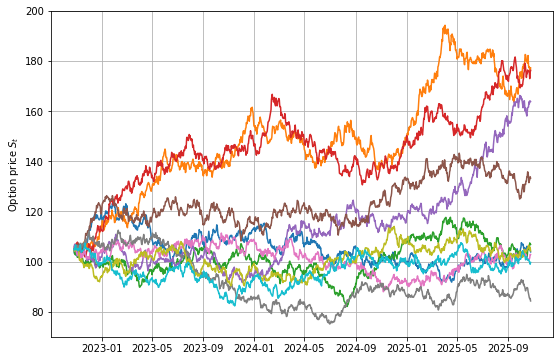
\includegraphics[width=0.7\linewidth]{figures/underlying_simulation}
\end{figure}

This implementation is not optimized in terms of speed, indeed it takes about 2 minutes to run 500 simulations.
A different approach, fully exploiting \texttt{numpy.array}s, could allow to shrink the execution time by a factor of 200.

\begin{ipython}
from datetime import date
from dateutil.relativedelta import relativedelta
from finmarkets import CreditCurve, call
from scipy.stats import norm
import numpy as np
import time

K = 110
sigma = 0.15
r = 0.03
T = 3
steps = 365*T
dt = 1/365
R = 0.4
Q = [0.9, 0.8, 0.7]
S0 = 105

obs_date = date.today()
dates = [obs_date + relativedelta(years=i+1) for i in range(T)]
cc = CreditCurve(obs_date, dates, Q)
t1 = time.time()
scenarios = 500
St = np.zeros(shape=(steps, scenarios))
St[0, :] = S0
ndps = np.zeros(shape=(steps,))
for i in range(1, steps):
    St[i, :] = St[i-1, :] * np.exp((r - 0.5 * sigma**2) * dt \
        + sigma* np.sqrt(dt) * norm.rvs(size=scenarios))
    ndps[i] = cc.ndp(obs_date+relativedelta(days=i-1)) - \
        cc.ndp(obs_date+relativedelta(days=i))

ts = ["{}y".format(t) for t in np.arange(T-dt, 0, -dt)]
cvas = np.zeros(shape=(steps, scenarios))
for s in range(scenarios):
    for j in range(len(ts)):
        cvas[j, s] = call(St[j, s], K, r, sigma, ts[j])*(1-R)*ndps[j]
cvas = np.sum(cvas, axis=0)
print (np.mean(cvas))
print (time.time() - t1)
\end{ipython}
\begin{ioutput}
2.464147656202549
129.0265169143676
\end{ioutput}
\end{solution}

\begin{question}
\label{ex:credit_var}
Consider a 1-years call with strike 110 EUR. The underlying initial price is 100 EUR with a volatility of 0.50. The risk-free rate is 0.03 flat. Compute the 99.9\% Credit VaR assuming a recovery rate of 40\% and default probabilities for the underlying of 30\% within next year.
\end{question}

\cprotEnv\begin{solution}

In order to increase the number of simulations the implemented code fully uses \texttt{numpy.array}.

\begin{ipython}
import numpy as np
from datetime import date
from dateutil.relativedelta import relativedelta
from finmarkets import CreditCurve
from scipy.stats import norm


K = 110
sigma = 0.50
r = 0.03
T = 1
steps = 365*T
dt = 1/365
R = 0.4
S0 = 100

obs_date = date.today()
cc = CreditCurve(obs_date, [obs_date + relativedelta(years=1)], [0.7])
scenarios = 10000
St = np.zeros(shape=(steps, scenarios))
St[0, :] = S0
ndps = np.zeros(shape=(steps,))
for i in range(1, steps):
    St[i, :] = St[i-1, :] * np.exp((r - 0.5 * sigma**2) * dt \
                                   + sigma* np.sqrt(dt) * norm.rvs(size=scenarios))
    ndps[i] = cc.ndp(obs_date+relativedelta(days=i)) - \
        cc.ndp(obs_date+relativedelta(days=i+1))

ts = ["{}y".format(t) for t in np.arange(T-dt, 0, -dt)]
EE = np.zeros(shape=(steps, scenarios))
for s in range(scenarios):
    EE[1:, s] = call(St[:-1, s], K, r, sigma, ts)*(1-R)*ndps[1:]
EE = np.sum(EE, axis=0)
print ("Credit VaR: {:.3f}".format(np.percentile(EE, 99.9)))\end{ipython}
\begin{ioutput}
Credit VaR: 26.281
\end{ioutput}

\begin{figure}[htbp]
\centering
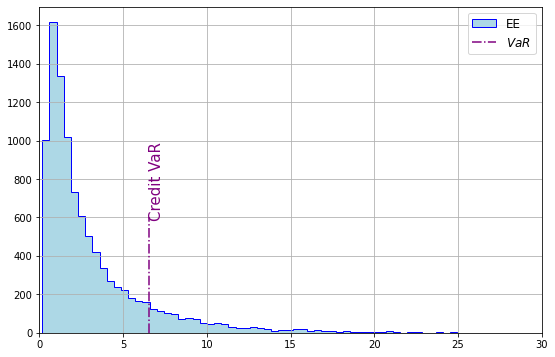
\includegraphics[width=0.7\linewidth]{figures/cr_var_ex}
\caption{Loss distribution to estimate Credit VaR measure of Ex.~\ref{ex:credit_var}.}
\end{figure}
\end{solution}







\chapter{Kernel Density Estimation}
\label{Kernel Density}

\section{Introduction}
Suppose we have some low dimensional data (1 or 2 variables). How do we start exploring them? Usually, one of the first steps is to plot their histogram to get a feeling of how they are distributed. Histograms are nice because they provide a fast and unambiguous way to visualize our data's probability distribution. However, they are discrete, and sometimes it is useful to have a smooth estimation of the underlying probability density function (PDF) at hand. Figure~\ref{fig:kde_example} shows an example of Kernel density estimate.

\pythoncodenon{code/kde_example.py}

\begin{figure}[htb]
\centering
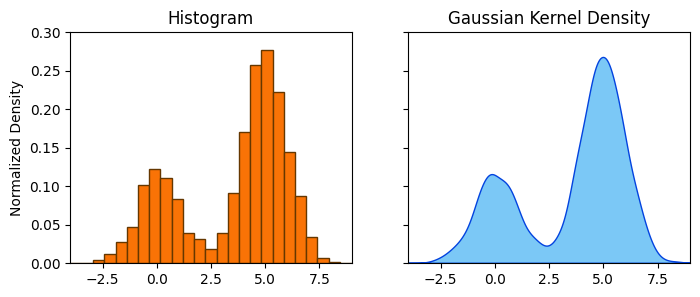
\includegraphics[width=0.75\textwidth]{figures/kde_example}
\caption{Left plot shows an histogram with a sampled distribution. Right plot the Gaussian kernal density estimate.}
\label{fig:kde_example}
\end{figure}

There are two ways to get a smooth PDF from your data.

The \emph{parametric} probability density estimation where we pick a common distribution (say a normal distribution), and we estimate its parameters (e.g., mean, standard deviation) from the data sample.
The \emph{nonparametric} probability such as kernel density estimation (KDE), that we will be discussing today.

\section{The Case of 1 Variable}
In the univariate case KDE is very straightforward. Here is how we'd do it. Assuming we have a set of $N$ samples $x_i=\{x_1,x_2,\ldots,x_N\}$, the KDE, $\hat{f}$, of the PDF is defined as:

\begin{equation}
\hat{f}(x,h)=\cfrac{1}{N}\sum_{i=1}^{N}K_h(x-x_i)
\end{equation}

Basically, in the kernel density estimation approach, we center a smooth scaled kernel function at each data point and then take their average. One of the most common kernels is the \emph{Gaussian kernel}:
\begin{equation}
K(u)=\cfrac{1}{\sqrt{2\pi}}\exp\left(-\cfrac{u^2}{2}\right)
\end{equation}

The $K_h$ is the scaled version of the kernel, i.e., $K_h(u)=\frac{1}{h}K(\frac{u}{h})$. The parameter $h$ of the kernel is called the \emph{bandwidth}, and this little number is a very critical determinant of our estimate's quality. As important as the kernel choice itself! By tweaking its value, we change the width of the kernel.

Kernel density estimation has two main difficulties:
\begin{enumerate}
\item optimal bandwidth estimation;
\item the varying data density makes regions of high data density requiring small bandwidths, and areas with sparse data needing large bandwidths.
\end{enumerate}

Here is a concrete example that sums all of the above assuming a trivial sample $X=\{1,2,3,4,7,9\}$.
And this is the corresponding output:

\begin{equation}
\hat{f}(x, 1)=\cfrac{1}{6}\left(
  \cfrac{e^{-\frac{1}{2}(x-9)^2}}{\sqrt{2\pi}}+
  \cfrac{e^{-\frac{1}{2}(x-7)^2}}{\sqrt{2\pi}}+
  \cfrac{e^{-\frac{1}{2}(x-4)^2}}{\sqrt{2\pi}}+
  \cfrac{e^{-\frac{1}{2}(x-3)^2}}{\sqrt{2\pi}}+
  \cfrac{e^{-\frac{1}{2}(x-2)^2}}{\sqrt{2\pi}}+
  \cfrac{e^{-\frac{1}{2}(x-1)^2}}{\sqrt{2\pi}}\right)
\end{equation}

The following implementation is based on the \texttt{sklearn.neighbors.KernelDensity} utility available in \texttt{python}.

\pythoncodenon{code/kde_one_variable.py}

In Figure~\ref{fig:kde_one_variable}, we plot both the individual Gaussian kernels, along with the kernel density estimate. The black dots are our data points and notice how they are at the kernels' center.

\begin{figure}[htb]
\centering
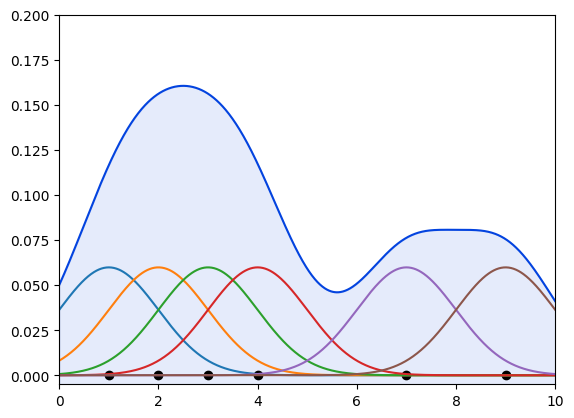
\includegraphics[width=0.75\textwidth]{figures/kde_one_variable}
\caption{In the plot are reported both the individual Gaussian kernels, along with the kernel density estimate for our sample. The black dots are our data points; notice how they are at the kernels' center.}
\label{fig:kde_one_variable}
\end{figure}

In Figure~\ref{fig:kde_bandwidth} the output of our own kernel density estimation for varying values of the bandwidth parameter $h$ is shown. The black dots at the bottom represent our sample data. Notice how for small values of the bandwidth parameter $h$, the KDE is rigged. But, as $h$ increases, the estimate gets smoother and smoother. The selection of the parameter $h$ is, as we have already said, very crucial.

\pythoncodenon{code/kde_bandwidth.py}

\begin{figure}[htb]
\centering
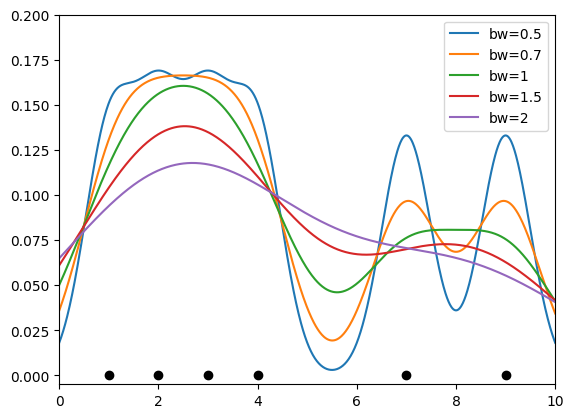
\includegraphics[width=0.75\textwidth]{figures/kde_bandwidth}
\caption{The plot shows how changing the bandwidth parameter affects the density estimate. For small values of $h$ the KDE is rigged. But, as it increases, the estimate gets smoother and smoother.}
\label{fig:kde_bandwidth}
\end{figure}

\subsection{Bandwidth Selection}

There are a number of ways to choose a bandwidth. \emph{Cross validation} is one, but for a much faster approach there are some rules of thumb you can refer to:
\begin{itemize}
\item Scott's Rule: $n^{-\frac{1}{d + 4}}$;
\item Silverman's Rule: $\left(\cfrac{n \cdot (d + 2)}{4}\right)^{-\frac{1}{d + 4}}$.
\end{itemize}

In both of these, $d$ is the dimensionality of your data, and $n$ is the number of data points you have. 
In our example the suggested bandwidth according to Silverman's rule should be 0.74.

\section{Other Kernels}

In principle, we could use whatever kernel we'd like, as long as it is symmetric, non-negative, and integrates to 1. However, our choice should take into consideration the underlying process that generates our data. In the following example, we use a \emph{cosine kernel} on the same data as before.

In Figure~\ref{fig:kde_cosine_kernel} our kernel density estimation for varying bandwidth parameter values $h$ using the cosine kernel.

\pythoncodenon{code/kde_cosine_kernel.py}

\begin{figure}[htb]
\centering
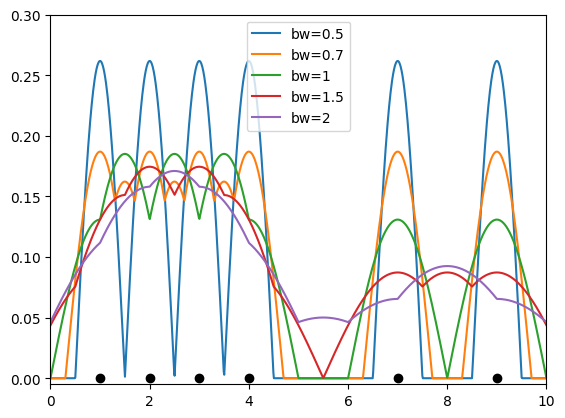
\includegraphics[width=0.75\textwidth]{figures/kde_cosine_kernel}
\caption{The plot shows how changing the bandwidth parameter affects the density estimate. For small values of $h$ the KDE is rigged. But, as it increases, the estimate gets smoother and smoother.}
\label{fig:kde_cosine_kernel}
\end{figure}

\section{KDE and S\&P500}

In this example we attempt to use Kernel Density Estimation techniques to generate a PDF, and then estimate how likely the stock market is to crash from a day to day basis.

So as a first step let's 500 price data (daily OHLC: Open-High-Low-Close) data into a Pandas dataframe
(I have saved in a csv file \href{https://raw.githubusercontent.com/matteosan1/finance_course/refs/heads/develop/input_files/SPX.csv}{SPY.csv}). 
Since we are trying to model the S\&P 500 daily returns, instead of the actual prices, we will use the super-handy \texttt{pct\_change()} function, and put the daily return data into a new column: 'pct\_change'.

It is always good practice to split your data into "training" and "test" sets. Let's say as we use 2009 to 2015's data as the training set, and anything that is 2016 onwards will be used as the test set.

\pythoncodenon{code/kde_spy.py}
\begin{ioutput}
2009-01-05 00:00:00 2015-12-31 00:00:00 2016-01-04 00:00:00 2024-09-24 00:00:00
\end{ioutput}

\begin{figure}[htb]
\centering
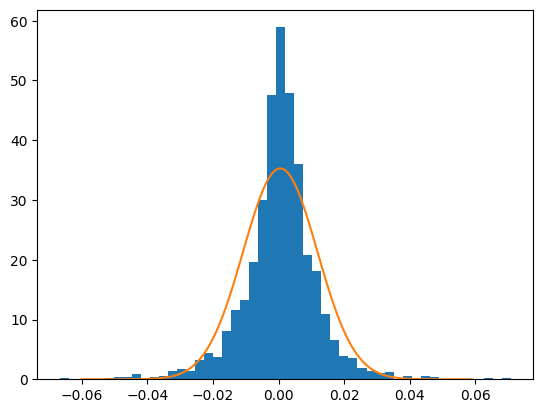
\includegraphics[width=0.7\textwidth]{figures/spy_distro}
\caption{Distribution of the S\&P 500 daily returns in the period 2009-2015.}
\label{fig:spy_distro}
\end{figure}

The histogram in Fig.~\ref{fig:spy_distro} looks like a mal-nourished normal distribution, looks too skinny. Although there are numerical techniques to determine how well (or bad) a PDF matches a distribution we settle for the by eye comparison.

\subsection{KDE Application}

To get a better estimate of the PDF we will be approaching the problem via Kernel Density Estimation. 
Our train\_returns is an 1D-array, meaning it has a shape of (rows,). However most sklearn functions require the data to be re-shaped to have 1 column, i.e. the shape needs to be (rows,1).

Next, the kde variable is loaded up with the Kernel Density object, then fitted with the \texttt{train\_returns\_arr} data.

You may notice that I specified the bandwidth parameter as 0.001. That is just my "guestimate" of a reasonable bandwidth value. Guestimating the bandwidth value is more art than science: if you do not get it right the first time, just change to another value and see if it improves. Feel free to experiment with other numbers for the bandwidth parameter - we will be optimizing this parameter later.

Now, \texttt{kde} is already fitted with the S\&P 500 daily returns data; this means it is a PDF on its own.
We can get the actual probabilities (log-probabilities in this case) values through the \texttt{KernelDensity.score\_samples()} function. Then calculating the actual PDF values is quite straight forward: just calculate the exponential values. Figure~\ref{fig:kde_kde_spy} shows the result.

\pythoncodenon{code/kde_kde_spy.py}

\begin{figure}[htb]
\centering
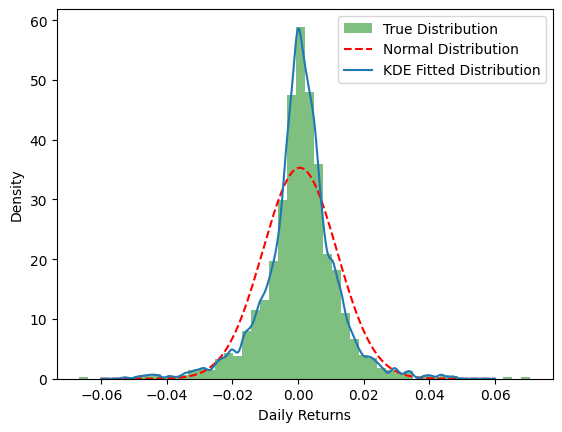
\includegraphics[width=0.75\textwidth]{figures/kde_kde_spy}
\caption{Distribution of the S\&P 500 daily returns in the period 2009-2015 with the KDE PDF.}
\label{fig:kde_kde_spy}
\end{figure}

The KDE Fitted Distribution PDF fits the True Distribution data much better compared to the Normal Distribution curve, i.e. it follows the shape of the True Distribution.

Unfortunately if you zoom into the tails, e.g. -0.02 to -0.06 or 0.02 to 0.06, you can see that the KDE fitted PDF overfits to the True Distribution. To illustrate what I mean, I re-produced the same chart below, but zoomed into one of the tails.

From Fig.~\ref{fig:kde_kde_spy_zoomed} we can see that the KDE Fitted Distribution curve was fooled by the random noise in the True Distribution data. It looks nothing like a "fat tail" distribution.

\begin{figure}[htb]
\centering
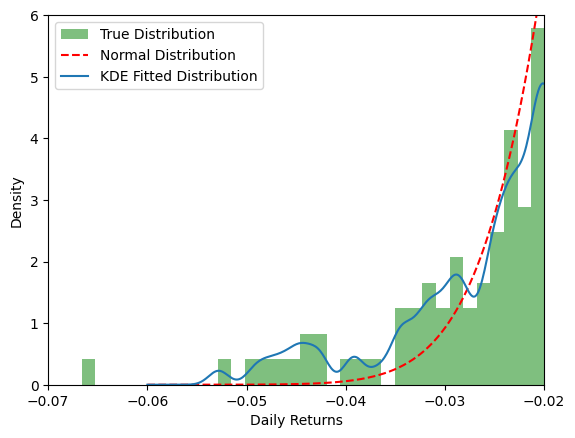
\includegraphics[width=0.75\textwidth]{figures/kde_kde_spy_zoomed}
\caption{Distribution of the S\&P 500 daily returns in the period 2009-2015 with the KDE PDF, zoomed on a tail.}
\label{fig:kde_kde_spy_zoomed}
\end{figure}

\subsection{Optimize the \texttt{KernelDensity} Object}

Luckily \texttt{sklearn} provides the \texttt{GridSearchCV} function: this can help us fine-tuning the \texttt{KernelDensity} parameters so that it generalize better to the noisy data.

\begin{finmarkets}
If you are not familiar with the \texttt{GridSearchCV} function, here is how you work with it: define a "parameter grid" that you want to optimize as a dictionary, for example:

\begin{ipythonbox}
# optimize bandwidth
params = {'bandwidth' : np.linspace(-0.0001, 0.01, 50)}    
                                                           # OR
# optimize bandwidth and kernel type
params = {
    'bandwidth' : np.linspace(-0.0001, 0.01, 30),
    'kernel': ['gaussian', 'epanechnikov', 'exponential']
         }
\end{ipythonbox}
Then run the function, like this:
\begin{ipythonbox}
grid = GridSearchCV(KernelDensity(), 
                    param_grid=params, 
                    cv=20).fit(train_returns_arr)
\end{ipythonbox}                    
Finally read the best parameters via \texttt{grid.best\_params\_}.
\end{finmarkets}

So we can optimize the bandwith (the parameter turns out to be 0.00412) and re-fit the distribution, see Fig.~\ref{fig:kde_opt_band}. 

\pythoncodenon{code/kde_opt_band.py}
\begin{ioutput}
{'bandwidth': 0.004122448979591837}
\end{ioutput}

\begin{figure}[htb]
\centering
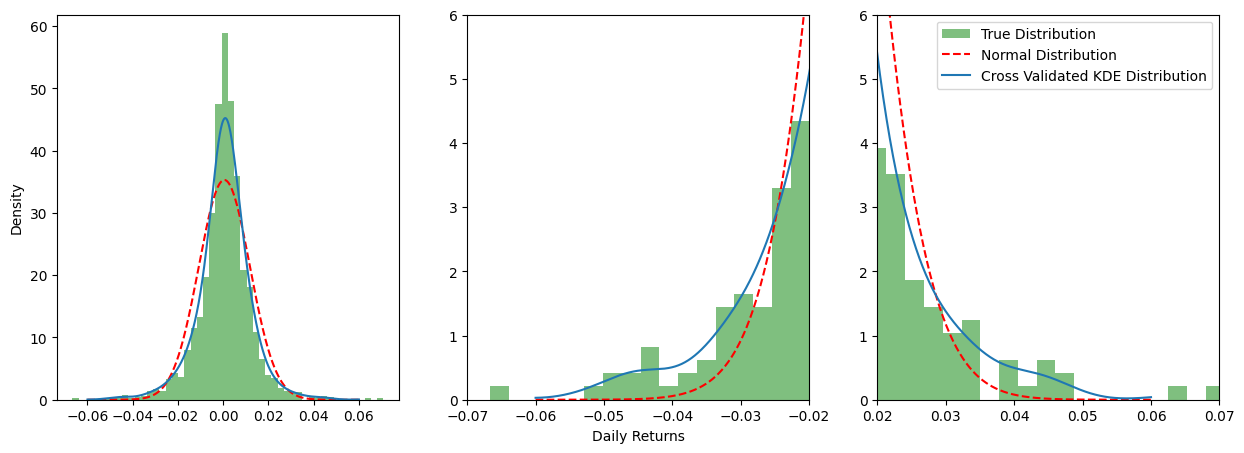
\includegraphics[width=0.9\textwidth]{figures/kde_opt_band}
\caption{Distribution of the S\&P 500 daily returns in the period 2009-2015 with the KDE PDF, zoomed on a tail.}
\label{fig:kde_opt_band}
\end{figure}

Is the optimized KernelDensity any better than before ?
At first glance, the KDE curve looks much better than before. It did not seem to overfit to the random noise at both left and right tails, as you can see by looking at the two right-most plots of Fig.~\ref{fig:kde_opt_band}.

This KDE PDF is by no means perfect, but much better than before.

\subsection{Market Crash Probability}

Let's calculate how likely the stock market will crash more than 4\% a day. Below we are going to use three different methods:
\begin{itemize}
\item using the actual probability, e.g. based on the number of times the S\&P 500 actually crashed more than 4\%;
\item using the optimized KDE's PDF;
\item modelling the stock market returns as a Normal Distribution (which we now know is NOT the right approach).
\end{itemize}

\pythoncodenon{code/kde_market_crash.py}
\begin{ioutput}
Actual probability:              0.568%
Best Fit KDE probability:        0.603%
Normal distribution probability: 0.017%
\end{ioutput}

Within 2009-2015 (our training set's time period), the S\&P 500 crashed (more than 4\%) from a day to day basis, 0.568\% of the time. The best fit (optimized) KDE predicted 0.603\%, not bad at all. But the normal distribution prediction of 0.017% is no where near the reality.

\subsubsection{About Calculating the KDE's Probabilities}

You may have noticed that I calculated the KDE's probabilities using the following:
\begin{ipythonnon}
crash_range = np.linspace(-0.1, -0.04, 1000)
best_kde_probs = np.exp(best_kde.score_samples(crash_range.reshape(-1,1)))
best_kde_probs_integrated = np.trapz(best_kde_probs, x=crash_range)
\end{ipythonnon}

Basically we are trying to calculate the probability of \texttt{train\_returns\_arr} having a value of less than -0.04. That means we need to calculate the probability of it having values between -1.0 and -0.04. This means we are looking for a CDF value:
\begin{equation}
\int_{-\infty}^{-0.04} KDE(x) dx
\end{equation}
(the lower limit of -1.0 is because the most the S\&P 500 can drop is dropping to zero, hence the \texttt{pct\_change()} would be -1.0, or -100\%).

The \texttt{KernelDensity} object does not include a CDF function, so we can only estimate its value by approximating the intergration, in this example I used \texttt{np.trapz()} function (trapz means trapezium rule).

In the code above, \texttt{crash\_range} ranges from -10\% to -4\%, instead of from -100\% and -4\%. -10\% is just an arbitarily small enough number that I chose as the lower limit of the integration, as the KDE's PDF would predict 0\% probability for anything smaller than -0.10 anyway.
 % da riguardare
\chapter{Machine Learning Theory}
\label{ch:neural-network}

In this Chapter we will see how machine learning techniques can be successfully applied to solve financial problems. We first do a quick tour on the theory behind neural networks and then see few examples and practical applications regarding regression and classification issues.

Beware this Chapter just scratches the surface of machine learning theory which has seen a huge development in the latest years leading to thousands of applications in many different fields.
    
\section{Neural Networks}\label{neural-networks}

Artificial Neural Networks (ANN or simply NN) are information processing models that are developed by inspiring from the working principles of the human brain. Their most essential property is \emph{the ability of learning from sample sets}.

\subsection{Neurons and Activation Functions}
The basic unit of an ANN is the neuron. It consists of weights ($w_i$) and takes in input real numbers ($x_i$). After the injection into a neuron all these inputs are individually weighted, added together (sometimes it is added also a bias $w_0$) and passed into the activation function $f$ which produces the final neuron output

\begin{equation}
\textrm{Inputs} = \sum_{i=1}^{N} x_i w_i + w_0 \rightarrow f(\textrm{Inputs}) = \textrm{Outputs}
\end{equation}
Figure~\ref{fig:neuron} shows an example of neuron.

\begin{figure}[htb]
	\centering
	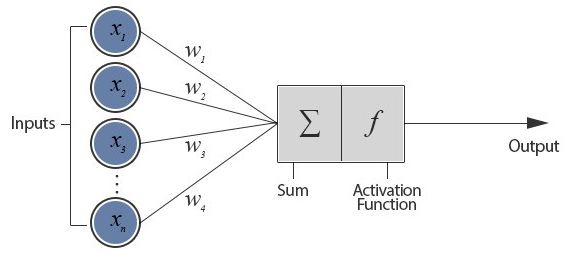
\includegraphics[width=0.45\textwidth]{figures/neuron}
	\caption{Model of an artificial neuron.}
	\label{fig:neuron}
\end{figure}

The activation function is the key ingredient to make neural networks non-linear models, indeed it is responsible to add non-linearity to the neuron output.

There are many different types of activation function:
\begin{itemize}
\item \emph{step function}: which returns just 0 or 1 according to the input value;
\item \emph{sigmoid}: which can be thought of as the continuous version of the step function;
\item \emph{hyperbolic tangent} (tanh);
\item \emph{rectified Linear Unit} (ReLU);
\item \emph{softplus};
\item \emph{softmax}: mainly used for ”classification” problems.
\end{itemize}

Figure~\ref{fig:act_func} reports graphs for various type of activations.
For a deeper discussion on activation functions see~\cite{bib:activation_function}.

\begin{figure}[htb]
\centering
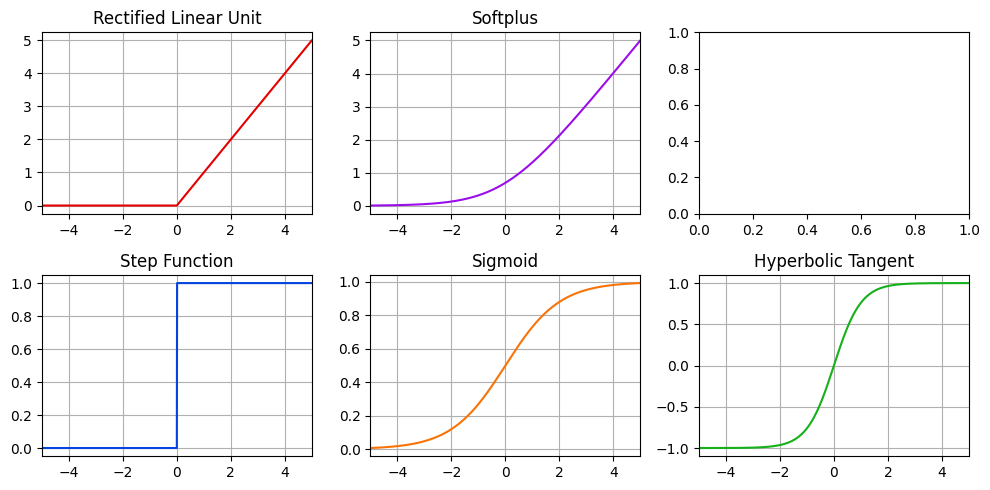
\includegraphics[width=0.90\textwidth]{figures/sigmoid}
\caption{Example graphs of various activation functions.}
\label{fig:act_func}
\end{figure}  

%When teaching children how to recognize a bus, we just tell them, showing an example: "This is a bus (or that is not a bus)." until they learn the concept of what a bus is. Afterwards, if a child sees new objects that she hasn't seen before, we could expect her to recognize correctly whether the new object is a bus or not.
%
%This is exactly the idea behind neuron training. Inputs from a \emph{training} set are presented to the neuron, one after the other, together with the correct output. During the process neuron weights are modified so that its response best matches the target output we provided.
%
%When an entire pass through all of the inputs is completed (an \emph{epoch}) the neuron has learned. Usually, to make it learn even better, the same training data is processed multiple times.
%
%After the training is completed, when an input vector $\mathbf{x}$, contained in the training set, is presented to the neuron, it will output approximately the correct value. With out of sample $\mathbf{x}$, the neuron will respond with an output close to those corresponding to other training vectors similar to $\mathbf{x}$.
%
%This kind of training is called \emph{supervised} because the input dataset is accompanied by the known targets (the true outputs), and we want our model to learn to predict the target from those input variables.
%
%Unfortunately using just a neuron is not too useful since with such a simple architecture is not possible to solve the interesting problems we would like to face. 
%The next step is to put together more neurons in \emph{layers} and connect those layers in more advanced configuration.

\subsection{Multilayered Networks}
\label{multi-layered-neural-networks}

To really make a neural network useful the number of employed neurons must be increased.
The architecture of such networks is called \textit{multilayered neural network} because the neurons are arranged in layers. Usually these networks are also \textit{fully connected} meaning that each neuron from a \emph{layer} is fed up to each node in the next. This kind of connection is repeated for each node down to the \emph{output layer}, For an example see Figure~\ref{fig:multilayered_nn}.

We should note that there can be any number of nodes per layer and there are usually multiple \emph{hidden layers} to pass through before ultimately reaching the output. The \textbf{only two architectural constraints} are: the neuron number in the input layer has to match the inputs number, and the amount of output layer nodes needs to match the desired target. 

\begin{figure}[htb]
\centering
\includegraphics[width=0.6\textwidth]{figures/multilayer.jpeg}
\caption{A multilayered neural network.}
\label{fig:multilayered_nn}
\end{figure}

\section{Neural Network Training}
\label{training-a-multilayered-neural-network}

When teaching children how to recognize a bus, we just tell them, showing an example: "This is a bus (or that is not a bus)." until they learn the concept of what a bus is. 
Afterwards, if a child sees new objects that she hasn't seen before, we could expect her to recognize correctly whether the new object is a bus or not.

This is exactly the idea behind \textit{network training}, the process by which the parameters of the model, i.e. neuron weights, are set to their optimal values. 
Inputs from a training set are presented to the neuron, one after the other, together with the correct output. During the process neuron weights are modified so that its response best matches the target output we provided. When an entire pass through all of the inputs is completed (an \emph{epoch}) the model has learned. Usually, to make it learn even better, the same training data is processed multiple times.

After the training is completed, when an input vector $\mathbf{x}$, contained in the training set, is presented to the NN, it will output approximately the correct value. With out of sample $\mathbf{x}$, the neuron will respond with an output close to those corresponding to other training vectors similar to $\mathbf{x}$.

This kind of training is called \emph{supervised} because the input dataset is accompanied by the known targets (the true outputs), and we want our model to learn to predict the target from those input variables.

In order to understand how the training works, let's imagine we have implemented a very simple model with
\begin{itemize}
\item 1 neuron in the input layer;
\item 2 neurons in a single hidden layer;
\item 1 neuron in the output layer.
\end{itemize}
For the activation function we are going to use softplus.

The training algorithm can be summarized as follows:
\begin{enumerate}
\item \textit{forward pass}: present the training dataset at the input layer and "propagate" it through the network as seen before (note the model parameters are initially set to random values);
\item \textit{loss}: calculate the difference between NN predicted and target output. There are many ways to estimate that difference: here we are going to use the \textit{quadratic difference}
\begin{equation}
L = \sum_{i=0}^N (\text{target}_i - \text{predicted}_i)^2
\end{equation}
\item \textit{backpropagation}: "adjust" the network parameters using \textit{gradient descent} algorithm to reduce the loss $L$;
\item repeat from the first step several times (epochs) until the loss has reached a reasonably small value.
\end{enumerate}

\subsection{Backpropagation}

To illustrate with a simple example how backpropagation works, let's imagine we need to determine $w_3, w_4$ and $b_3$ of our example network, see Figure~\ref{fig:training}.

\begin{figure}[htb]
	\centering
	\includegraphics[width=0.9\textwidth]{figures/training_nn}
	\caption{An example of a multilayered neural network, we need to determine the model parameters at the last neuron.}
	\label{fig:training}
\end{figure}

As said we need to apply the gradient descent algorithm to \textit{minimize} the loss function.

The most efficient way to find the minimum of a function with respect of some parameters is change those parameters following the "direction" given by the gradient.
For our example this means that we need to compute $\frac{\partial L}{\partial w_3}$, $\frac{\partial L}{\partial w_4}$ and $\frac{\partial L}{\partial b_3}$ and update the parameters as
\begin{equation}
w_3^{new} = w_3^{old} - \alpha \cdot \frac{\partial L}{\partial w_3}
\end{equation}
where $\alpha$ is the \textit{learning rate} a constant determining the size of the steps the algorithm takes toward the minimum of the loss function.

The three derivatives can be computed thanks to the \textit{chain rule} which states that given $f(x(t))$:
\begin{equation}
\frac{\partial f}{\partial t} = \frac{\partial f}{\partial x}\cdot \frac{\partial x}{\partial t}
\end{equation}

So following the notation of Figure~\ref{fig:training} and remembering that $L = \sum_{i=0}^N (t_i - p_i)^2$ and $p_i = N^i_1\cdot w_3 + N^i_2\cdot w_4 + b_3$ we get
\begin{equation}
\begin{gathered}
\frac{\partial L}{\partial w_3} = \sum_i \frac{\partial L}{\partial p_i} \frac{\partial p_i}{\partial w_3} = \sum_i -2\cdot(t_i-p_i)\cdot \frac{\partial p_i}{\partial w_3} = \sum_i -2\cdot(t_i-p_i)\cdot N^i_1 \\
\frac{\partial L}{\partial w_4} = \sum_i -2\cdot(t_i-p_i)\cdot N^i_2 \\
\frac{\partial L}{\partial b_3} = \sum_i -2\cdot(t_i-p_i)\cdot 1
\end{gathered}
\end{equation}

Figure~\ref{fig:learning_rate} shows how the convergence of the parameter $b_3$ optimization changes as function of the learning rate. Larger $\alpha$ makes the algorithm to find the optimal value faster.

Nevertheless when the learning rate is too large, the algorithm stops being a "descending" process and starts behaving erratically. Here a list of the possible pitfalls:
\begin{itemize}
\item overshooting the minimum: a large learning rate causes the algorithm to take steps so big that it leaps over the optimal point entirely;
\item divergence: if the learning rate is high enough, each subsequent step takes you further away from the center (the gradients get larger as you move away from the minimum, larger gradients lead to even larger steps);
\item perpetual oscillation: it bounces back and forth between the walls of the cost function, never reaching the bottom. This prevents the model from ever converging.
\end{itemize}

\begin{figure}[htb]
	\centering
	\includegraphics[width=0.8\textwidth]{figures/learning_rate}
	\caption{Convergence of the $b_3$ parameter as a function of the gradient descent learning rate $\alpha$.}
	\label{fig:learning_rate}
\end{figure}

A very similar process can be applied to all the other neurons to adjust all the model parameters. As we go further back the network the derivatives becomes a little bit more complicated, but thanks to the chain rule the entire backpropagation algorithm can be expressed in matricial form becoming essentially a linear algebra problem.

In Appendix~\ref{sec:nn_from_scratch} is reported an implementation from scratch of a neural network, backpropagation included.

\subsection{Hyper-parameters Setting}
\label{neural-network-design}

%There is no rule to guide developers into the design of a neural network in terms of number of layers and neurons (the so called \emph{hyper-parameters}). 
%
%One popular method for hyper-parameter optimization is the \emph{grid search}. A list of possible values for each hyper-parameter is defined, then the model is run multiple times, each time with a different combination of the hyper-parameter values. In the end the set giving the best result is taken. This is the most thorough way of selecting the neural network architecture but it is also the most computationally intense.
%In the end a \emph{trial and error} strategy is what is implemented anyway, and the solution giving the best accuracy is selected, although without an exhaustive check of all the possibilities.
%
%In general a larger number of nodes is better to catch highly structured data with a lot of feature although it may require larger training sample to work correctly. As a rule of thumb a \emph{NN with just one hidden layer and a number of neurons averaging the inputs and outputs} is sufficient in most cases.

Every NN has three types of layers: input, hidden, and output and creating its architecture means coming up with values for the number of layers of each type, the number of nodes in each of these layers and the choice of the activation function type.
Unfortunately there is not standard and accepted method for selecting the so-called \emph{hyper-parameters}. 

\subsubsection*{Input and Output Layers}

Every NN has exactly one of both, no exceptions. 

The number of input neurons is completely and uniquely determined once you know the shape of your training data. Specifically, the number of neurons in the input layer is equal to the number of features (columns) in your data. 

The size of the output layer instead is completely determined by function dimension in case of a \textbf{regressor} model (see Section~\ref{regression}) or by the number of classes if it is a \textbf{classifier} model (see Section~\ref{classification}).

\subsubsection*{The Hidden Layers}

First examine how to determine the number of hidden layers to use with the neural network.

\paragraph{Hidden Layer Number}
If your data is linearly separable, then you don't need any hidden layers at all. Of course, you don't need a NN to resolve your data either, but it will still do the job.

Beyond that, there's a mountain of commentary on the question of hidden layer configuration in NNs. One issue within this subject on which there is a \textbf{consensus} is the performance difference from adding additional hidden layers: the situations in which performance improves with a second (or third\ldots) hidden layer are very few i.e. \emph{one hidden layer is sufficient for the large majority of problems}. Table~\ref{tab:nn} summarizes the capabilities of neural network architectures with various hidden layers.

\begin{center}
	\begin{table}[htbp]
		\begin{tabularx}{\textwidth}{|c|X|}%|p{0.3\linewidth}|p{0.65\linewidth}|}
		\hline
		%\vspace{1mm}
		Number of Hidden Layers & Result\xdef\tempwidth{\the\linewidth}\\
		\hline
		%\vspace{0.2\baselineskip} 
		0 & \multicolumn{1}{|m{\tempwidth}|}{Only capable of representing linear separable functions or decisions.} \\
		\hline
		%\vspace{0.2\baselineskip}
		1 & \multicolumn{1}{|m{\tempwidth}|}{Can approximate any function that contains a continuous mapping from one finite space to another.} \\
		\hline
		%\vspace{0.5\baselineskip}
		2 & \multicolumn{1}{|m{\tempwidth}|}{Can represent an arbitrary decision boundary to arbitrary accuracy with rational activation functions and can approximate any smooth mapping to any accuracy.} \\
		\hline
		%\vspace{0.1\baselineskip}
		More than 2 &  \multicolumn{1}{|m{\tempwidth}|}{Additional layers can learn complex representations (sort of automatic feature engineering)} \\
		\hline
	\end{tabularx}
	\vspace{2mm}
	\caption{Determining the number of hidden layers.}
	\label{tab:nn}
\end{table}
\end{center}

\paragraph{Hidden Neuron Number}

Deciding the number of neurons in the hidden layers is a very important part of deciding your overall neural network architecture. Though these layers do not directly interact with the external environment, they have a tremendous influence on the final output, hence their number must be carefully considered.

In order to secure the network ability to generalize the number of nodes has to be kept as low as possible. If you have a large excess of nodes, your network becomes a memory bank that can recall the training set to perfection, but does not perform well on samples that was not part of the training set. This is usually referred to as \emph{over-fitting}.

On the other hand using too few neurons in the hidden layers will result in something called \emph{under-fitting}. It occurs when the number of neurons is inadequate to detect the signals in a complicated data set.

Obviously, some compromise must be reached between too many and too few neurons in the hidden layers. There are some empirically derived rules of thumb:
\begin{itemize}
\item the number of hidden neurons should be between the size of the input layer and the size of the output layer;
\item the number of hidden neurons should be 2/3 the size of the input layer, plus the size of the output layer~\cite{bib:heaton};
\item the number of hidden neurons should be less than twice the size of the input layer~\cite{bib:heaton};
\item a rough approximation can be obtained by the geometric pyramid rule~\cite{bib:master} (e.g. for a three layer network with $n$ input and $m$ output neurons, the hidden layer would have $\sqrt{n\cdot m}$ neurons);
\item over-fitting can usually be prevented by keeping the number of neurons below~\cite{bib:hagan}:
\begin{equation*}
	N_h = \frac{N_s}{\alpha\cdot(N_i+N_o)}
\end{equation*}
where $N_i$ = number of input neurons, $N_o$ = number of output neurons, $N_s$ = number of samples in training data set, $\alpha$ = an arbitrary scaling factor usually between $[2-10]$. 
You want to limit the number of free parameters in your model (\emph{degree}) to a small portion of the degrees of freedom in your data which is the number of samples times the  dimensions in each sample or $N_s\cdot(N_i+N_o)$. So $\alpha$ is a way to indicate how general you want your model to be, or how much you want to prevent over-fitting (with 10 giving the safest architecture).
\end{itemize}

In sum, for most problems, one could probably get decent performance (even without a second optimization step) by setting the hidden layer configuration using just two rules:
\begin{enumerate}
\item the number of hidden layers equals one; 
\item the number of neurons in that layer is the mean of the neurons in the input and output layers.
\end{enumerate}

\subsubsection{Activation Function}

The activation function choice mainly depends on the actual model performance.

In some cases *sigmoid* and, at a lesser extent, *hyperbolic tangent* may suffer from the **vanishing gradient** problem.

Sigmoid squashes input values into the range $(0,1)$. The function's derivative, which is used during backpropagation to calculate the gradient (see later), has a bell shape and approaches zero as the input gets large (either very positive or very negative).

When gradients are multiplied layer-by-layer during backpropagation through a deep network, these small derivatives rapidly compound, causing the gradients for the initial layers to become very small.

Consequently, the weights in the early layers update very little, or "vanish," making the network unable to learn meaningful features from the input data.

ReLU function solves this issue since its derivative is 1 for every input greater than 0.

If you are dealing with classification models instead, you should go for the softmax function, which "transform" the neuron output into actual probabilities for the sample to belong a certain class.

\subsubsection*{Optimization of the Network Configuration}

Previous rules provide a good starting point to consider. Ultimately, the selection of an architecture for your neural network will come down to a smart \emph{trial and error}. 

\paragraph{Pruning}
The term \emph{pruning} describes a set of techniques to trim network size (by nodes, not layers) to improve computational and sometimes resolution performance. 
The gist of these techniques is removing nodes from the network during training by identifying those nodes which, if removed from the network, would not noticeably affect network performance. To get a rough idea of which nodes are not important it is enough to look at the weight matrix after training and consider to remove the nodes with weights very close to zero. 
Obviously, if you use a pruning algorithm during training, then begin with a network configuration that has excess of nodes.

\paragraph{Genetic Algorithms}

Another approach involves a set of techniques called "genetic algorithms" that try a small subset of the potential options (random number of layers and nodes per layer). It then treats this population of options as "parents" that create children by combining/mutating one or more of the parents much like organisms evolve. The best children and some random OK children are kept in each generation and, over generations, the fittest survive.

For about 100 or fewer parameters (such as the choice of number, type of layers, and number of neurons per layer), this method is super effective. It can be used to create a number of potential network architectures for each generation and training them partially till the learning curve can be estimated. After a few generations, you may want to consider the point in which the train and validation start to have significantly different error rate (over-fitting) as your objective function for choosing children. It may be a good idea to use a very small subset of your data (10-20\%) until you choose a final model to reach a conclusion faster. Also, use a single seed for your network initialization to properly compare the results. 10-50 generations should yield great results for a decent sized network.

\begin{attention}
\subsubsection{Technical Note}
\label{technical-note}

Neural network training and testing is performed using two modules: \texttt{keras}~\cite{bib:keras} (which in turn is based on a Google open source library called \texttt{tensorflow}~\cite{bib:tensorflow}) and \texttt{scikit-learn}~\cite{bib:scikit} which provides many useful utilities.
\end{attention}

\section{Regression and Classification}
\label{regression-and-classification}

Neural network applications can be categorized into two main classes: \emph{classification} and \emph{regression}. Let's see their characteristics and differences.

\subsection{Regression}
\label{regression}

Regression is the process of finding hidden correlations between dependent variables. It helps in predicting market trends, house prices,~$\ldots$

The goal is to find the mapping function between the input variables ($x$) and the \emph{continuous} output variable ($y$), that is to find the best fit which can predict the output.

As an example suppose we want to do weather forecasting. The model is trained on past data, and on the basis of today's inputs can predict the weather for future days. In general whenever we are dealing with function approximations this kind of techniques can be applied.

\subsection{Classification}
\label{classification}

Classification is the process of finding a function which helps in dividing the input dataset into classes based on its characteristics. The goal is to find the mapping function between the input ($x$) and the \textbf{discrete} output ($y$) or, equivalently, to find the decision boundary which can divide the dataset into different classes.

A typical classification problem is the \emph{email spam detection}. The model is trained on different parameters using millions of emails, and whenever it receives a new email, it checks whether is spam or not. Classification algorithms can also be used in speech recognition, car plates identification,~\ldots

\section{Function Approximation Example}
\label{function-approximation}

Let's design an ANN which is capable of learning the functional form underlying a set of data. For this example the training sample is generated as a two columns array: $x$ (input), $f(x)$ (target output) where $f(x)$ is unknown. The dataset is saved in \href{https://raw.githubusercontent.com/matteosan1/finance_course/refs/heads/develop/input_files/function_approx.csv}{function\_approx.csv}. 

Before embarking into the actual training the sample undergoes to a transformation in order to have all the inputs (and outputs) with the same scale. This sample transformation is called \emph{scaling}, and is done to provide the NN with "equalized" inputs since it could be fooled by very large or small numbers giving unstable results.

There are various methods available for data scaling in \texttt{scikit-learn}, the most important being:
\begin{itemize}
\tightlist
\item \emph{StandardScaler}: scales features such that the distribution is centered around 0, with a standard deviation of 1. It is not quite good if data is not normally distributed (i.e. no Gaussian distribution);
\item \emph{MinMaxScaler}: shrinks the range such that it becomes between 0 and 1 (or -1 to 1 if there are negative values in the first place). It is influenced heavily by outliers (i.e. extreme values);
\item \emph{RobustScaler}: similar to the previous one but it instead uses quantile ranges, so that it is robust against outliers. It doesn't take the median of the original sample into account and only focuses on the regions where the bulk data is. Consider that \textbf{robust} doesn't mean immune or invulnerable and that the purpose of scaling is not to remove outliers.
\end{itemize}

Figure~\ref{fig:scalers} reports the different transformations on the distribution of the target outputs. Which one to use depends on the particular case under study: in the actual example we are going to use the \texttt{MinMaxScaler}.

\begin{figure}[htb]
\centering
\includegraphics[width=0.9\textwidth]{figures/scalers}
\caption{Effect of different kind of scalers in the target output distribution.}
\label{fig:scalers}
\end{figure}

\pythoncode{code/machine_learning_function_approx_preprocess.py}
\begin{ioutput}
Data before scaling 3.893108764379634, 4.514195769839021
The same data after scaling 0.0, 1.0
\end{ioutput}

In the following we will use complex networks just for illustration, but no attempt in optimizing the layout has been done at all.
In our first example two hidden layers with 15 and 5 neurons respectively and a \texttt{tanh} activation function are used, see Fig,~\ref{fig:ann_1}. The \texttt{inputs} parameter has to be set to 1 since we have just one single input, the \texttt{x} value.
The training will last 100 epochs and the mean squared error is used as loss function. Note the parameter \texttt{batch\_size} in the \texttt{fit} command; it can be useful in those circumstances where if we will feed the complete dataset during the training process to the model and then will try to do a backpropagation for all examples at once, we might run out of memory, and each training epoch may take too long to execute. To avoid a situation like this, we need to split our dataset indeed into batches.

\pythoncode{code/machine_learning_function_approx.py}

\begin{ioutput}
Epoch 1/100
10/10 .................... 1s 5ms/step - loss: 0.2124
Epoch 2/100
10/10 .................... 0s 4ms/step - loss: 0.1755 
...
Epoch 99/100
10/10 .................... 0s 6ms/step - loss: 0.0184 
Epoch 100/100
10/10 .................... 0s 6ms/step - loss: 0.0191 	
\end{ioutput}

\begin{figure}[htb]
\centering
\includegraphics[width=0.9\textwidth]{figures/ann_1.png}
\caption{Graphical representation of the ANN used to approximate the unknown function.}
\label{fig:ann_1}
\end{figure}

The training output shows: a counter with the current epoch number, the computed loss which is evaluated using the chosen method and the timing. When the training is completed we can evaluate how good it is \textbf{using the loss value.}

Since it takes some time to generate data samples and training, it is always advisable to save them in a file since it may be needed to load it many times during the NN development. 
Also both the training model and the actual scalers need to be stored in files in order to use them for later predictions. 

\begin{ipythonnon}
import joblib

model_name = 'func_approx'
model.save(job_name)

joblib.dump(scale_X, model_name + "_x_scaler.save")
joblib.dump(scale_y, model_name + "_y_scaler.save")
model.save(model_name)
\end{ipythonnon}

The \texttt{fit} command returns a useful dictionary with all the relevant values to check the network training i.e. efficiency and loss as a function of the epochs. We have stored this dictionary in the \texttt{history} variable.

\subsection{Model Prediction}

To get predictions from our trained model is not completely straightforward since we have scaled both input and target values.

As we will see NN are \textbf{not capable} of \textit{extrapolate} results so it is mandatory that the input we present to the NN has the same "characteristics" as the ones used in the training (e.g. if the input variables has a certain range of variability, \textbf{our test input must lay on the same range or the NN will spit out nonsensical results}).

So to make a prediction we need:
\begin{enumerate}
\item scale the input $x$ with the \textbf{very same} transformation used before the training (that's why we saved it...)
\begin{equation*}
x \rightarrow f_{\text{scaleX}}(x) = x_s
\end{equation*}
\item pass $x_s$ to the NN to get a prediction $y_s = NN(x_s)$;
\item the NN has been constructed to return a \textit{scaled output} (since we also scaled $y$ before the training), so we need to \textbf{anti-scale} the NN prediction with the inverse transformation to get a meaningful result
\begin{equation*}
f^{-1}_{\text{scaleY}}(y_s) \rightarrow \tilde{y}
\end{equation*}
\end{enumerate}

\begin{ipythonnon}
x0 = np.array(df['X'].iloc[0])
true_value = df['y'].iloc[0]

x_transf = scaler_X.transform(x0.reshape(-1, 1))
y_pred = scaler_y.inverse_transform(model.predict(x_transf, verbose=0))

print (f"Predicted value (true): {y_pred[0][0]} ({true_value})")
print (f"Difference: {abs(y_pred[0][0]-true_value)}")
\end{ipythonnon}
\begin{ioutput}
Predicted value (true): 4.422266006469727 (4.0)
Difference: 0.42226600646972656
\end{ioutput}

\subsubsection{Hallucinations}

In the context of machine learning models, \textit{hallucination} often translates to extrapolation failure: the model makes a highly confident but nonsensical prediction when given an input that is far outside the distribution of its training data.

As an example let's calculate another prediction from the model this time without scaling the input.

\begin{ipythonnon}
x0 = np.array(df['X'].iloc[-1])
x_transf = scaler_X.transform(x0.reshape(-1, 1))
true_value = df['y'].iloc[-1]

y_pred_x0 = scaler_y.inverse_transform(model.predict(x0.reshape(-1,1), verbose=0))
y_pred_x_transf = scaler_y.inverse_transform(model.predict(x_transf, verbose=0))

print (f"Predicted value w/ scaling: {y_pred_x_transf[0][0]} {true_value}")
print (f"Predicted value w/o scaling: {y_pred_x0[0][0]} {true_value}")
\end{ipythonnon}
\begin{ioutput}
Predicted value w/ scaling: 4.035444736480713 3.996373043598315
Predicted value w/o scaling: 5.130277633666992 3.996373043598315
\end{ioutput}

The second prediction, the one without the scaling is vastly off the true value.

As a second example of hallucination let's try to approximate with a simple network a dataset made of samples from a parabola with some Gaussian noise on top.

\begin{ipythonnon}
import numpy as np, tensorflow as tf

from tensorflow.keras.models import Sequential
from tensorflow.keras.layers import Dense, Input

def true_function(X):
    return X**2

X_train = np.linspace(0, 5, 50).reshape(-1, 1)
noise = np.random.normal(0, 2, X_train.shape)
y_train = true_function(X_train) + noise

X_test = np.linspace(0, 15, 100).reshape(-1, 1)
y_true = true_function(X_test)

model = Sequential([Input(shape=(1,)),
                    Dense(32, activation='relu'),
                    Dense(16, activation='relu'),
                    Dense(1)])

model.compile(optimizer='adam', loss='mse')
history = model.fit(X_train, y_train, epochs=1000, verbose=0, validation_split=0.1)

y_pred = model.predict(X_test).squeeze()
\end{ipythonnon}

Figure~\ref{fig:hallucination1} clearly shows how outside the training region the model predicts values quite off the real distribution.

\begin{figure}[htb]
	\centering
	\includegraphics[width=0.9\textwidth]{figures/hallucination1}
	\caption{Hallucination in a simple example where we try to approximate a parabola plus Gaussian noise..}
	\label{fig:hallucination1}
\end{figure}

\subsection{Overfitting}
\label{sec:overtraining}

A \emph{perfect} model would lead to a zero loss so the lower these number the better is our training. 
Model performance improves with the number of epochs in the training, since the NN has more chances to learn the input features. 
To get an idea of what is going on in Figure~\ref{fig:training_vs_epochs} is shown the actual function we want to approximate and different predictions obtained with the same architecture but various number of epochs (i.e. 5, 100, 1000, 50000). Clearly the agreement improves with the number of epochs.

\begin{figure}[htb]
\centering
\includegraphics[width=0.9\textwidth]{figures/training_vs_epoch}
\caption{Prediction of the target $f(x)$ using different number of epochs in the training (5, 100, 1000 and 50000) respectively.}
\label{fig:training_vs_epochs}
\end{figure}

Clearly the agreement improves with a higher number of epochs which means that the NN had more opportunities to adapt the weights and reduce the loss.

Notice that it is not fair to estimate model performance with the same dataset used for the training: usually the original data is split into two parts named training and testing samples. We will see this in later examples.

\subsubsection{Bias - Variance Trade Off}

When a function $f$ is approximated with a model $h^*$, the "distance" between the model and the truth represents the \textbf{bias} of associated to my model.
If I repeat the training with independent samples I most likely obtain slightly different models ($h_1, h_2, h_3\ldots$). The dispersion of the different model results represents its \textbf{variance}.
Figure~\ref{fig:bias_variance} illustrates an exemplified situation.

\begin{figure}[htb]
	\centering
	\includegraphics[width=0.3\textwidth]{figures/bias_variance}
	\caption{Bias and variance of the model $h$ approximating the function $f$.}
	\label{fig:bias_variance}
\end{figure}

In general \textbf{simple models corresponds to high bias regressions} i.e. they are not capable of catching the full complexity of the original dataset.
Contrary \textbf{more complex models are characterized by a large variance}, since they tend to over-parametrize the original model.

\subsubsection{Epochs vs Model Complexity}

The inherent complexity of a neural network is defined by its architecture (number of layers, neurons, etc.). However, the effective complexity, or how well the model fits the training data, is determined by both the architecture and the training time (epochs).

You can associate the increasing number of epochs in the training with the increasing effective model complexity because additional epochs give the optimization algorithm more time to fine-tune the model's parameters to the training data.

This relationship drives the transition from a high-bias state to a high-variance state.
In the initial epochs, the model is simple or "low-capacity" in the sense that it hasn't used its full potential. The error is dominated by high bias. Each epoch pushes the model's parameters further down the loss surface, making a better fit to the training data. The model reduces its simplistic assumptions (lowers the bias) and captures more detail in the training set.

As you move past the point where the model has learned the main patterns, continued training (more epochs) causes the model to seek out and incorporate the remaining tiny imperfections (i.e. noise).
The model's predictions become overly sensitive to the specific data points used for training. This sensitivity to training set fluctuations is the definition of high variance, which leads to overfitting and poor generalization on new, unseen data.

Sometimes overfitting is explained by saying that the model is "trained too well" on the particular dataset used in the process. This means that the NN mostly memorized data, and its performance accounts for a large accuracy within the training sample but a low accuracy in similar but independent datasets. 

To check for possible overfitting it is required to split the available sample in at least two parts: training and testing (e.g.~80\% and 20\%) and to use the former to perform the training and the latter to cross-check performance. If the two losses are comparable the NN is OK, otherwise if the loss on the training is much smaller than the testing we had overfitting.

The following example illustrates the issue. We get 10 samples from an unknown distribution, 4 for training and six for testing. We first try to model the samples
using the simplest model, a line. The loss results to be 0.003 for the training and 0.018 for the testing sample so we can say the the model underfit the data, Figure~	\ref{subfig:underfitting}.

We then use a third degree polynomial (a more complex model) to approximate the unknown distribution and we get a 0 loss for the training set (one and only one cubic pass through 4 points), while for the testing set it explodes to 103.6. Clearly the model overfits the sample, Figure~\ref{subfig:overfitting}. 

\begin{figure}[htb]
	\centering
	\subfloat[The linear model is too simple to catch the feature of the dataset.\label{subfig:underfitting}]{%
		\includegraphics[width=0.5\textwidth]{figures/underfitting}
	}
	\subfloat[Increasing the model complexity to a third degree polynomial introduces overfitting.\label{subfig:overfitting}]{%
		\includegraphics[width=0.5\textwidth]{figures/overfitting}
	}
	\caption{Illustrative plot to show the connection between model complexity and bias variance trade-off.}
	\label{fig:underfitting_overfitting}
\end{figure}

In the original example, when using 50000 epochs i.e. the most complex model tried, the overfitting check results in
\begin{ipythonnon}
from tensorflow.keras.models import load_model
from sklearn.model_selection import train_test_split

train_X, test_X, train_y, test_y = \
    train_test_split(scaled_X, scaled_y, test_size=0.2)

model50000 = load_model(f"func_50000epochs.keras")

eval_train = model50000.evaluate(train_X, train_y)
eval_test = model50000.evaluate(test_X, test_y)

print(eval_train)
print(eval_test)	
\end{ipythonnon}
\begin{ioutput}
25/25 .................... 0s 4ms/step - loss: 1.1323e-06
7/7 .................... 0s 12ms/step - loss: 1.1882e-06 
1.1509513342389255e-06
1.1420811460993718e-06
\end{ioutput}
The performance with the two datasets are comparable, hence no overfitting occurred.
 
\subsubsection{How to Mitigate Overfitting}

The most common techniques to reduce overfitting focus on limiting the model's complexity or injecting noise into the training process.
\begin{itemize}
\item \textit{Early Stopping} is a very simple yet crucial technique: training is halted when the performance on a separate validation set starts to degrade, preventing the model from over-optimizing for the training data's noise;
\item \textit{Dropout}: randomly deactivates a fraction of neurons during each training step. This forces the network to learn more robust, less dependent features. It is designed to avoid co-adaptation:
 if several neurons always fire together to correct an error, they develop complex co-dependencies. This makes the network highly specialized non-robust because these neurons only work in tandem and often learn noise from the training data, leading to overfitting; with dropout no single neuron can rely on another specific neuron being present. Each neuron is forced to learn features that are useful in conjunction with any random subset of other neurons.
\item \textit{Regularization techniques}: L1 and L2 regularizations are widely used; they add a penalty term to the loss function based on the magnitude of the model's weights, encouraging simpler weight distributions.
	\begin{itemize}
		\item L1 Regularization (Lasso) adds a penalty $\lambda\sum_i |w_i|$; it can force the weights of irrelevant features to become exactly zero (i.e. automatic feature selection), creating a model where less important features are completely eliminated.
		\item L2 Regularization (Ridge) adds a penalty $\lambda\sum_i w_i^2$; drives weights towards zero, but rarely makes them exactly zero. It prefers models where all features contribute a little, rather than a few features contributing a lot. This helps distribute the weight values more evenly, resulting in a model that is less sensitive to small changes in the training data.
\end{itemize}
\end{itemize}

\subsection{Why Am I Getting Different Results ?}

In applied machine learning, we run an algorithm on a dataset to get a model. The model is then used to predict outputs from inputs given a dataset. Unlike the models that we may be used to, neural networks may not be entirely deterministic.
The resulting machine learning models may be different each time they are trained. In turn, the models may make different predictions, and when evaluated, may have a different level of error or accuracy. This is to be expected and might even be a feature of the algorithm, not a bug.
In the following the major sources of difference are listed and analyzed.

\subsubsection{Stochastic Learning Algorithm}

Neural network models are not deterministic but rather stochastic. This means that their behavior incorporates elements of randomness.
Nevertheless stochastic does not mean random: the machine learning algorithms are not learning a random model. They are learning a model conditional on the dataset you have provided. Instead, the specific small decisions made by the algorithm during the learning process can vary randomly.

The impact is that each time the stochastic machine learning algorithm is run on the same data, it learns a slightly different model. In turn, the model may make slightly different predictions, and when evaluated using error or accuracy, may have a slightly different performance.

The random initial weights allow the model to try learning from a different starting point in the search space each time and allow the learning algorithm to “break symmetry” during learning. The random shuffle of examples during training ensures that each gradient estimate and weight update is slightly different.

Nevertheless the randomness used by learning algorithms can be controlled. For example, you set the seed used by the pseudo-random number generator to ensure that each time the algorithm is run, it gets the "same randomness".

This is not a good approach in practice (apart from tutorials or lectures). Since there is no best seed for a stochastic machine learning algorithm you can summarize the performance of these models by fitting multiple final models on your dataset and averaging their predictions.

\subsubsection{Evaluation Procedure}

There may be differences in the training data due to sample splitting.
A train-test split involves randomly assigning rows to either be used to train the model or evaluate the model to meet a predefined train or test set size.

\subsubsection{Differences Caused by Platform}

Different results can arise from running the same algorithm on the same data on different computers.
This can happen even if you fix the random number seed to address the stochastic nature of the learning algorithm and evaluation procedure. The cause in this case is the platform or development environment used to run.

Some of the possible specific causes are:
\begin{itemize}
\tightlist
\item system architecture, e.g. CPU or GPU;
\item operating system, e.g. MacOS or Linux;
\item underlying math libraries, e.g. LAPACK or BLAS;
\item \texttt{python} of library version, e.g. 3.6 or 3.7, \texttt{scikit-learn} 0.22 or 0.23.
\end{itemize}

Honestly, the effect is usually very small in practice (at least in my experience) as long as major software versions are used.

\section{Image Recognition Neural Network}
\label{neural-net-to-recognize-handwritten-digits}

The difficulties of visual pattern recognition becomes immediately apparent if you attempt to write a computer program to recognize digits like those in Fig.~\ref{fig:mnist}.

\begin{figure}[b]
\centering
\includegraphics[width=0.5\textwidth]{figures/mnist_100_digits}
\caption{MNIST sample of handwritten digits.}
\label{fig:mnist}
\end{figure}

Simple intuition about how we discern shapes (e.g. a 9 has a loop at the top, and a vertical stroke in the bottom right) turns out to be not so simple to express algorithmically. When you try to make such rules precise, you quickly get lost in a morass of exceptions, caveats, and special cases so that it seems hopeless.

Neural networks approach the problem in a different way. They take a large number of handwritten digits and develop a system which can learn from those.

By increasing the number of training examples, the network can learn more and more about handwriting, and so improve its accuracy. So while it has been shown just 100 training digits in Fig.~\ref{fig:mnist}, a better handwriting recognizer could be certainly built by using thousands or millions training examples (\textbf{as we have seen above neural nets are not capable of extrapolating results, hence in general it won't recognize a digit written in some strange way not included in the training sample !!!}).

\subsection{Convolutional Layer}

An image can be thought of as a matrix:
\begin{itemize}
\item \emph{grayscale}: each pixel is represented as a number ranging from 0 (black) to 255 (white);
\item \emph{colored}: each pixel is a triplet of numbers ranging from 0 to 255 and indicating the intensity of Red, Green and Blue (RGB) component.
\end{itemize}

Every image can be transformed by applying \emph{kernels} (sometimes referred to as filters). Such kernels are matrices which are \emph{convolved} with the original image, this operation is explained in Fig.~\ref{fig:convolution} and essentially means that each pixel of the kernel is multiplied by the corresponding image pixel and the results are summed together. The process is repeated many times in order to cover the entire image surface.

\begin{figure}[htb]
\centering
\includegraphics[width=0.8\textwidth]{figures/convolution}
\caption{Example of convolution between a kernel and an image.}
\label{fig:convolution}
\end{figure}

Starting from the original image shown in Fig.~\ref{subfig:kernel_orig} it can be seen how by applying various filters (i.e. different definition of the kernel matrix) can be extracted the main features of the image. Figures~\ref{subfig:kernel_hor}, \ref{subfig:kernel_ver} and~\ref{subfig:kernel_blur} show examples of the so called \emph{Sobel} kernels detecting horizontal and vertical edges and of the Gaussian blurring.

\begin{figure}[!p]
\centering
\subfloat[Original image of a road.\label{subfig:kernel_orig}]{%
	\includegraphics[width=0.45\textwidth]{figures/via_gray}
	}\quad
\subfloat[Sobel kernel for horizontal edges.\label{subfig:kernel_hor}]{%
	\includegraphics[width=0.45\textwidth]{figures/hor}
	}\\
\subfloat[Sobel kernel for vertical edges.\label{subfig:kernel_ver}]{%
	\includegraphics[width=0.45\textwidth]{figures/ver}
	}\quad
\subfloat[Gaussian blurring kernel.\label{subfig:kernel_blur}]{%
	\includegraphics[width=0.45\textwidth]{figures/blur}
	}
\caption{Example application of different kernels on an image.}
%\label{fig:dummy}
\end{figure} 

To implement image recognition in machine learning a new kind of network has to be used, the Convolutional Neural Network (CNN). It is based on a different kind of layer (\emph{convolutional layer}) which instead of applying predefined filters like the ones seen before, learns the specific ones which are better in highlighting the training dataset features. If we want to make a parallelism between NN and CNN, the former parameters are the neuron weights while in the latter the those are the elements of the kernel matrices.

Stacking convolutional layers prove to be very effective, and allows to learn both low (e.g. lines) and high level features (e.g. complex shapes or even specific objects).

The CNN output won't be a single number but rather a list containing the probabilities that an image belongs to each class, thanks to the \texttt{softmax} activation at the last layer. 
Next we define the CNN architecture, see Fig.~\ref{fig:cnn2d}, to explore its capabilities the sample provided with the \texttt{mnist} module will be used.

\pythoncode{code/machine_learning_cnn.py}
\begin{ioutput}
Epoch 1/5
1875/1875 [==============================] - 19s 10ms/step - loss: 2.0868
Epoch 2/5
1875/1875 [==============================] - 18s 10ms/step - loss: 0.3320
Epoch 3/5
1875/1875 [==============================] - 18s 10ms/step - loss: 0.2153
Epoch 4/5
1875/1875 [==============================] - 18s 10ms/step - loss: 0.1891
Epoch 5/5
1875/1875 [==============================] - 18s 10ms/step - loss: 0.1799
<keras.callbacks.History at 0x7f07b05d0350>
\end{ioutput}

\begin{attention}
\subsubsection{Pooling}

Looking closely to the convolutional neural network implementation we can notice new kind of layers never used before, in particular the \texttt{MaxPooling2} layer.

Convolutional layers in a CNN systematically apply filters to input images in order to create feature maps that summarize the main characteristics of the sample.

A limitation of such maps is that they record the precise position of features in the input. This means that small movements in its position will result in a different feature map. This can happen with cropping, rotation, shifting, and other minor changes to the input image.

Imagine a program that looks for car plates in pictures taken by a speed radar: cars won't be in the same position in the frame so there may be differences in the classification of similar (but not equal) pictures.

A common approach to address this problem is called \emph{down sampling}. 
This is where a lower resolution version of an input signal (e.g. the picture) is created that still contains the large or important structural elements, without the finer detail that may not be as useful to the task.

Down sampling can be achieved using a pooling layer.
It involves selecting kind of a filter to be applied to the feature maps. The pooling operation size is smaller than the feature map; specifically, it is almost always 2×2 pixels. This means that the pooling layer will always reduce the size of each feature map by a factor of 2, e.g. each dimension is halved. For example, a pooling layer applied to a feature map of 6×6 (36 pixels) will result in an output pooled feature map of 3×3 (9 pixels).

\begin{center}
\includegraphics[width=0.6\textwidth]{figures/MaxpoolSample2}
\end{center}

The most common pooling operation are:
\begin{itemize}
\tightlist
\item Average Pooling: calculate the average value for each patch on the feature map;
\item Maximum Pooling (or Max Pooling): calculate the maximum value for each patch of the feature map.
\end{itemize}
\end{attention}

\begin{figure}[htb]
\centering
\includegraphics[width=0.9\textwidth]{figures/cnn_2d}
\caption{Graphical representation of the CNN developed to recognize handwritten digits.}
\label{fig:cnn2d}
\end{figure}

Let's see how well our NN predicts \texttt{mnist} testing digits.

\begin{ipythonnon}
test_images = mnist.test_images()
test_labels = mnist.test_labels()

predictions = model.predict(test_images[:10])

print ("Tesing on MNIST digits...")
print("Predicted: ", np.argmax(predictions, axis=1)) 
print("Truth:     ", test_labels[:10])
\end{ipythonnon}
\begin{ioutput}
Tesing on MNIST digits...
Predicted:  [7 2 1 0 4 1 4 4 6 9]
Truth: [7 2 1 0 4 1 4 9 5 9]
\end{ioutput}

Since the last but one digit has lower probability let's check the returned list to see which other number have non-zero probability.

\begin{ipython}
for i, p in enumerate(predictions[-2]):
    print("9th digit:", [f"dig {i}: {p:.3f}"])
\end{ipython}
\begin{ioutput}
9th digit: ['dig 0: 0.0000', 'dig 1: 0.0000', 'dig 2: 0.0000', 
            'dig 3: 0.0000', 'dig 4: 0.0000', 'dig 5: 0.0001', 
            'dig 6: 0.9999', 'dig 7: 0.0000', 'dig 8: 0.0000', 
            'dig 9: 0.0000']
\end{ioutput}

%So the second ranked digit is a 6 (which can be confused with a five if the lower loop is almost closed).

The NN performance can be checked using your own calligraphy. 

Open your favorite image editor (e.g. Paint, GIMP,\ldots) and create a 200x200 pixels canvas. With the help of the mouse (or a pen) draw a digit and save it as a png file.
Before passing the image to the NN it has to be transformed to match the size and characteristics of those used in the training. This is done with an ad-hoc function, \texttt{transform\_image}, shown below.

\begin{ipythonnon}
import numpy as np
from PIL import Image

def transform_image(image_filename, size=(28,28)):
    image = Image.open(image_filename)
    grayscale_image = image.convert('L')
    grayscale_image = grayscale_image.resize(size, resample=Image.LANCZOS)
    return np.array(grayscale_image)

filenames = ['four.png', 'five.png']
for f in filenames:
    test_image = np.expand_dims(transform_image(f), axis=3)
    predict = model.predict(test_image)
    print ("Predicted: ", np.argmax(predict, axis=1))
    print("%:", [f"{p[np.argmax(p)]) for p in predict]:.3f}")
    print(["f{p:.2f}" for p in predict[0]])
\end{ipythonnon}
\begin{ioutput}
Predicted:  [4]
%: ['0.802']
['0.00', '0.00', '0.00', '0.00', '0.80', '0.00', '0.00', '0.20', '0.00', 
'0.00']

Predicted:  [5]
%: ['0.981']
['0.00', '0.00', '0.00', '0.01', '0.00', '0.98', '0.00', '0.01', '0.00', 
'0.00']
\end{ioutput}
The handwritten images used in this test are shown in Fig.~\ref{fig:test_images}.

\begin{figure}[htb]
\centering
\includegraphics[width=0.2\textwidth]{figures/four.png}
\includegraphics[width=0.2\textwidth]{figures/five.png}
\caption{Test handwritten digits used in the example.}
\label{fig:test_images}
\end{figure}

\subsection{Handwritten Digits with \texttt{Network}}

We can use the \texttt{Network} class to cross-check the classification of handwritten digits from the MNIST dataset (like it has been done in Sec~\ref{neural-net-to-recognize-handwritten-digits}) and it is made up of
\begin{itemize}
\item Input layer: will have 784 neurons corresponding to the each pixels in the 28x28 input images;
\item Two hidden layers: will have 100 and 50 neurons each with tanh activation;
\item Finally the output layer: will have 10 neurons corresponding to the ten digit classes with softmax activation.
\end{itemize}

The sample has been pre-processed by scaling each image in the range [0,1] (from the usual [0,255] of gray-scale images), also each matrix is flatten i.e. converted the $X$ array from (60000, 28, 28) to (60000, 784). Finally the array has been transposed such that each example image is a column.

\pythoncodenon{code/machine_learning_mnist_from_scratch.py}

\begin{ioutput}
epoch 1/35  error=0.23756977869124812
epoch 2/35  error=0.09585384173050779
epoch 3/35  error=0.0778832146987061
...
epoch 34/35  error=0.010464489201745728
epoch 35/35  error=0.010179050058617526

predicted value: 7 (prob. 0.947)
true value: 7

predicted value: 6 (prob. 0.856)
true value: 2

predicted value: 1 (prob. 0.969)
true value: 1
\end{ioutput}

\section{Remarks on Artificial Intelligence}

A neural network is a \emph{black box} in the sense that while it can approximate any function, studying its structure won't give you any insights on the functional form of the function being approximated.

As an example, one common use of neural networks on the banking business is to classify loaners on "good payers" and "bad payers". You have a matrix of input characteristics $C$ (sex, age, income\ldots) and a vector of results $R$ ("defaulted", "not defaulted"\ldots). When you model this using a neural network, you are supposing that there is a function $f(C)=R$, in the proper sense of a mathematical function. This function $f$ can be arbitrarily complex, and might change according to the evolution of the business, so you can't derive it by hand.

Then you use the Neural Network to build an approximation of $f$ that has an error rate that is acceptable to your application. This works, and the precision can be arbitrarily small, you can expand the network, fine tune its training parameters and get more data until the precision hits your goals.

The black box issue is: the approximation given by the neural network will not give you any insight on the form of $f$. There is no simple link between the weights and the function being approximated. 

Plus, from a traditional statistics viewpoint, a neural network is a non-identifiable model: given a dataset and network architecture, there can be two neural networks with different weights but exactly the same result. This makes the analysis very hard.
Needless to say, debugging NN results is even harder given this lack of interpretability. So use with caution machine learning models since they can be quite misleading.
  
\chapter{Machine Learning Applications}
\label{ch:neural-network-apps}

\section{Black-Scholes Call Option Price}
\label{black-scholes-call-options}

The first financial machine learning application concerns European call options pricing: we will implement a neural network capable of approximate the Black-Scholes pricing formula

\begin{equation} 
P_\textrm{call} = F_\textrm{BS}(M, r, \sigma, \mathrm{ttm})
\end{equation}

The first step consists of generating the training sample, made of volatility ($\sigma$)-rate ($r$) pairs (for simplicity we set moneyness ($M = S/K$ ) and time to maturity (ttm) to 1). The target value is the call price, computed using the BS formula.

\begin{ipythonnon}
import pandas as pd

from finmarkets import call

data = []
for r in np.arange(0.01, 0.11, 0.001):
    for sigma in np.arange(0.1, 0.6, 0.005):
       data.append({'rate':r, 'vol':sigma, 'price':call(1, sigma, r, 1)})

df = pd.DataFrame(data)
df.to_csv("bs_training_sample.csv")
\end{ipythonnon}
\begin{ioutput}
	rate           vol         price
	count  10000.000000  10000.000000  10000.000000
	mean       0.059500      0.347500      0.165274
	std        0.028868      0.144338      0.055387
	min        0.010000      0.100000      0.044852
	25%        0.034750      0.223750      0.119389
	50%        0.059500      0.347500      0.165476
	75%        0.084250      0.471250      0.212097
	max        0.109000      0.595000      0.277071
\end{ioutput}

\textbf{Beware that this time we have TWO input parameters (rate and volatility)}. See Figure~\ref{fig:ann_2} for a graphical representation of the designed ANN.

\begin{figure}[htb]
\centering
\includegraphics[width=0.9\textwidth]{figures/ann_2.png}
\caption{Graphical representation of the ANN used to approximate the Black and Scholes option price function.}
\label{fig:ann_2}
\end{figure}

\begin{ipythonnon}
X_scaled = scale_X.fit_transform(df[['rate', 'vol']])
Y_scaled = scale_Y.fit_transform(df[['price']])
	
X_train, X_test, Y_train, Y_test = train_test_split(X_scaled, 
                                                    Y_scaled, test_size=0.2)

model = Sequential()
model.add(Dense(20, input_dim=2, activation='relu'))
model.add(Dense(8, activation='relu'))
model.add(Dense(1, activation='relu'))

model.compile(loss='mse', optimizer='adam')
model.fit(X_train, Y_train, epochs=1500, verbose=1)
\end{ipythonnon}
\begin{ioutput}
Epoch 1/1500
250/250 [==============================] - 1s 1ms/step - loss: 0.0583
Epoch 2/1500
250/250 [==============================] - 0s 1ms/step - loss: 0.0042
...
Epoch 1499/1500
250/250 [==============================] - 0s 2ms/step - loss: 4.5252e-07
Epoch 1500/1500
250/250 [==============================] - 0s 2ms/step - loss: 4.8000e-07
<keras.callbacks.History at 0x7efd8c4dd7d0>
\end{ioutput}

\begin{ipythonnon}
import joblib

eval1 = model.evaluate(X_train, Y_train)
print(f'Training: {eval1}')

eval2 = model.evaluate(X_test, Y_test)
print(f'Test: {eval2}')

job_name = 'bs_model'
model.save(job_name)
joblib.dump(scale_X, job_name + "_x_scaler.save")
joblib.dump(scale_Y, job_name + "_y_scaler.save")
\end{ipythonnon}
\begin{ioutput}
250/250 [==============================] - 0s 1ms/step - loss: 5.9946e-07
Training: 5.994579055368376e-07
63/63 [==============================] - 0s 2ms/step - loss: 6.0690e-07
Test: 6.06896833232895e-07
\end{ioutput}

As you can see the training and testing samples give roughly the same loss value so we can be reasonably sure that there hasn't been \emph{over-fitting}.
After the training is completed we can evaluate graphically how good it is by plotting the difference between predicted and actual output as a function of the input parameters, see Figure~\ref{fig:vol_rate}. 
The gibbous structure of the relative error distribution, shown by Fig.~\ref{subfig:rel_err}, most likely can be flatten out with longer (most precise) training. The large peak in the low rate/volatility region is instead due to the decreasing price of the call; the absolute error (see Fig.~\ref{subfig:abs_err}) is indeed quite flat in that region and the decreasing price (it actually tends to zero (see Fig.~\ref{subfig:shape}) boosts the relative error.

\begin{figure}[!htp]
\centering
\subfloat[Black-Scholes price (at-the-money call). \label{subfig:shape}]{%
	\includegraphics[width=0.7\textwidth]{figures/bs_shape}
	}\\[30pt]
\subfloat[Relative error between predicted and actual price. \label{subfig:rel_err}]{%
	\includegraphics[width=0.5\textwidth]{figures/vol_rate}
	}
\subfloat[Absolute error between predicted and actual price. \label{subfig:abs_err}]{%
    \includegraphics[width=0.5\textwidth]{figures/vol_rate_abs_err}
	}
\caption{Neural network performance.}
\label{fig:vol_rate}
\end{figure}

Say we want to know the price of an at-the-money, 1 year call when the risk-free rate is 0.015 and the underlying volatility 0.234:

\begin{ipython}
import numpy as np

from finmarkets import call
from keras.models import load_model

model = load_model(job_name)
scale_X = joblib.load(job_name + "_x_scaler.save")
scale_Y = joblib.load(job_name + "_y_scaler.save")

rv = np.array([[0.015, 0.234]])
X = scale_X.transform(rv)
call_price = call(1, rv[0][1], rv[0][0], 1)
prediction = model.predict(X)
prediction = scale_Y.inverse_transform(prediction)[0][0]

print (f'{rv.tolist()} => {prediction:.4f} (expected {call_price:.4f})')
\end{ipython}
\begin{ioutput}
[[0.015, 0.234]] => 0.0999 (expected 0.1001)
\end{ioutput}

It is very important to remember that a \textbf{NN cannot extrapolate}.
Indeed if you try to predict the price of a call from rate and volatility outside the training \emph{phase space} (i.e. with values that aren't in the intervals used in the training), say \(r = 0.22\) and \(\sigma = 0.01\)\ldots{}

\begin{ioutput}
[[0.22, 0.01]] => 0.1583 (expected 0.1975)
\end{ioutput}

\section{Model Calibration}\label{model-calibration}

To use a certain model to solve real-world problems it is necessary to \emph{calibrate} it. This means that model parameters are derived directly from current market values. 

\begin{attention}
\subsubsection{Historical vs. Implied Volatility}
\label{historical-vs.-implied-volatility}
	
\emph{Historical volatility} is the realized volatility of an asset over a previous time period. It is determined by measuring the standard deviation of its price during that time period.
	
\emph{Implied volatility} is the expected future volatility of an asset that is implied by the current price of market products involving it.
In contrast to historical volatility, which looks at prices in the past, it looks toward the future and is often interpreted as the market's expectation for the future volatility of an asset.
	
Volatility shifts as market goes through different regimes. Thus, historical volatility may not be an accurate estimate of future. Implied volatility instead takes into account all information used by market participants to determine market prices and can give indications on the future behavior.
\end{attention}

Assume we need to estimate the \emph{implied volatility} of a security in real time. For such a task is enough to train a NN similar to the previous one which is designed to approximate the following function

\begin{equation} 
\sigma = F^{-1}_\textrm{BS}(P_\textrm{call}, m, r, \mathrm{ttm})
\end{equation}
\noindent
which is the inversion of the BS formula returning the volatility given the option price.

In this case calibration means to determine a Black-Scholes formula parameter (the volatility) from the market prices of the options and their characteristics.

The training sample created before can be re-used by swapping the dataframe columns to have in input rate and price and as target the output the volatility. 
Indeed we have never made any assumption on the functional form of the expression to approximate but just relied on the capability of NN to learn from the dataset.
This is very convenient to estimate quantities which are otherwise complicated to compute (i.e. there is no analytic formula to get these parameters).
 
\begin{ipython}
import pandas as pd

df = pd.read_csv("bs_training_sample.csv")
scale_X = MinMaxScaler()
scale_Y = MinMaxScaler()
X_scaled = scale_X.fit_transform(df[['rate', 'price']])
Y_scaled = scale_Y.fit_transform(df[['vol']])

X_train, X_test, Y_train, Y_test = train_test_split(X_scaled, 
                                                    Y_scaled, test_size=0.2)

model = Sequential()
model.add(Dense(20, input_dim=2, activation='relu'))
model.add(Dense(8, activation='relu'))
model.add(Dense(1, activation='relu'))

model.compile(loss='mse', optimizer='adam')
model.fit(X_train, Y_train, epochs=1500, verbose=1)
\end{ipython}
\begin{ioutput}
Epoch 1/2000
8000/8000 [==============================] - 0s 14us/step - loss: 0.1339
Epoch 2/2000
8000/8000 [==============================] - 0s 4us/step - loss: 0.1052
...
Epoch 1499/1500
250/250 [==============================] - 0s 2ms/step - loss: 3.8106e-07
Epoch 1500/1500
250/250 [==============================] - 0s 2ms/step - loss: 3.1316e-07
<keras.callbacks.History at 0x7efd8c5dea10>
\end{ioutput}

Provided our training includes the correct call market price range we can estimate the implied volatility. For example if the risk-free rate is 2\% and the current price is 0.15 

\begin{ipythonnon}
eval1 = model.evaluate(X_train, Y_train)
print(f'Training: {eval1}')

eval2 = model.evaluate(X_test, Y_test)
print(f'Test: {eval2}')
\end{ipythonnon}
\begin{ioutput}
250/250 [==============================] - 0s 1ms/step - loss: 2.8773e-07
Training: 2.8773044391527947e-07
63/63 [==============================] - 0s 2ms/step - loss: 2.9526e-07
Test: 2.9526071898544615e-07
\end{ioutput}

\begin{ipythonnon}
rv = np.array([[0.02, 0.15]])
prediction = model.predict(scale_X.transform(rv))
volatility = scale_Y.inverse_transform(prediction)[0][0]

print ('{rv.tolist()} => {volatility:.4f} (expected call price {call_m(1, volatility, 
	           0.02, 1):.4f})')
\end{ipythonnon}
\begin{ioutput}
[[0.02, 0.15]] => 0.3557 (expected call price 0.1499)
\end{ioutput}
\noindent
The expected call price (0.1499) derived using the implied volatility is in excellent agreement we the "market price" (0.15).

\section{Bankruptcy Prediction}
A company faces bankruptcy when it is unable to pay off its debts. The Taiwan Economic Journal has listed the details of company bankruptcy for the years 1999 to 2009 based on the business regulations of the Taiwan Stock Exchange which is a financial institution with over 900 listed companies. The dataset includes 94 numerical attributes that help understand the possibility of bankruptcy.

This ANN application aims at analyzing the possibility of whether an organization would face bankruptcy. Beside that a couple more concepts are analyzed in this example:
\begin{itemize}
\item \emph{imbalanced datasets}: is a situation when there is an unequal distribution of classes in a dataset. It can be solved by either up-sampling (i.e. introducing minority class samples) or down-sampling (i.e. reducing majority class to match the size of minority class);
\item finding the best attributes to work with through feature selection (i.e. it will be shown how programmatically pick the best features).
\end{itemize}

The input dataset can be downloaded from \href{https://raw.githubusercontent.com/matteosan1/finance_course/refs/heads/develop/input_files/bankruptcy.csv}{bankruptcy\_data.csv}
\begin{ipython}
import pandas as pd
	
data = pd.read_csv("bankruptcy_data.csv")
pd.options.display.max_columns=100
pd.options.display.max_rows=10
pd.set_option('display.float_format', f'{:.2f}')
	
print (data.head())
\end{ipython}
\begin{ioutput}
Net Worth Turnover Rate (times)  Revenue per person  \
0                          0.03                0.03   
1                          0.03                0.01   
2                          0.01                0.03   
3                          0.03                0.02   
4                          0.04                0.06   
...                        
\end{ioutput}

Given the very large number of available features it could be useful to remove those which present high correlation with other features and therefore cannot bring much improvement to NN performance.

Two techniques can be used: either perform a principal component analysis on the dataset and just keep the highest ranked feature of the most significant components~\ref{sec:pca} or compute the correlation matrix of the features, set a threshold and remove all the attributes above this value.

Here the latter method is used, choosing a correlation threshold of $|\rho|\geq 0.95$.

\begin{ipythonnon}
corr_mat = data.corr()
corr_mat = corr_mat.iloc[1:, 1:]
	
drop_list = {}
for i in range(len(corr_mat.columns)):
    for j in range(i):
        if abs(corr_mat.iloc[i, j]) >= 0.95:
            if corr_mat.columns[j] not in drop_list:
                drop_list.setdefault(corr_mat.columns[j], []) \
                    .append(corr_mat.columns[i])

for d in drop_list:
    print (d)
\end{ipythonnon}
\begin{ioutput}
ROA(C) before interest and depreciation before interest
ROA(A) before interest and % after tax
Operating Gross Margin
Pre-tax net Interest Rate
After-tax net Interest Rate
Net Value Per Share (B)
Net Value Per Share (A)
Persistent EPS in the Last Four Seasons
After-tax Net Profit Growth Rate
Debt ratio %
Operating Profit Per Share (Yuan)
Per Share Net profit before tax (Yuan)
Current Liabilities/Liability
Current Liabilities/Equity
Realized Sales Gross Margin
Borrowing dependency
Current Liability to Equity
\end{ioutput}
\noindent 
By analyzing \texttt{drop\_list} it can be checked where the maximum correlation happens.

Those 17 attributes are highly correlated with others in the dataset, therefore they do not bring additional discrimination power to the network and can be safely discarded. To check the effect of removing columns from the dataset it should be compared the performance of the NN with and without the selected attributes, here for simplicity this step will be skipped.

\begin{ipythonnon}
data = data.drop(drop_list, axis=1)
y = data['Bankrupt?']
X = data.drop(['Bankrupt?'], axis=1)
\end{ipythonnon}

\subsection{Unbalanced Datasets}

\begin{ipythonnon}
print (data['Bankrupt?'].value_counts())
\end{ipythonnon}
\begin{ioutput}
0    6599
1     220
Name: Bankrupt?, dtype: int64
\end{ioutput}

From the above check it is apparent that the dataset is highly imbalanced. The main problem with imbalanced classification is that there are too few examples of the minority class for a model to effectively learn the decision boundary. In this case it has been decided to reduce the problem by oversampling with the Synthetic Minority Oversampling Technique (SMOT)~\cite{bib:smot}. 

\begin{attention}
Oversampling could be in principle achieved by simply duplicating samples from the minority class in the training dataset prior to fitting a model. This would balance the class distribution but wouldn't provide any additional information to the model since it is merely a duplication of the existing information.
	
An improvement to this trivial strategy is to synthesize new samples from the minority class, a type of data augmentation that can be very effective.
SMOT algorithm works as follows: a random sample from the minority class is chosen. Then $k$ of the nearest neighbors for that sample are found (typically $k=5$) and one of them is randomly selected. Finally a synthetic sample is created at a randomly chosen point between the two samples still in the feature space.
Figure~\ref{fig:smote} shows a graphical representation of the algorithm.

This procedure can be used to create as many synthetic samples for the minority class as are required. 
The approach is effective because new synthetic samples are plausible, that is, are relatively close in feature space to existing samples from the minority class.

A general downside of the approach is that synthetic samples are created without considering the majority class, possibly resulting in ambiguous samples if there is a strong overlap for the classes.
\end{attention}

\begin{figure}[htb]
\centering
\includegraphics[width=0.7\textwidth]{figures/smote}
\caption{Graphical representation of the SMOT algorithm.}
\label{fig:smote}
\end{figure}

In \texttt{python} SMOT is implemented in \texttt{imblearn.over\_sampling} module.

\begin{ipythonnon}
from imblearn.over_sampling import SMOTE
	
oversample = SMOTE()
X_sm, y_sm = oversample.fit_resample(X, y)
print (y_sm.value_counts())
\end{ipythonnon}
\begin{ioutput}
1    6599
0    6599
Name: Bankrupt?, dtype: int64
\end{ioutput}

The last step to prepare the dataset for the analysis is its normalization which is necessary since each column ranges very differently.

\begin{ipythonnon}
from sklearn.preprocessing import StandardScaler
from sklearn.model_selection import train_test_split

scaler = StandardScaler()
X_sm = scaler.fit_transform(X_sm)

X_train, X_test, y_train, y_test = train_test_split(X_sm, y_sm, test_size=0.2)
\end{ipythonnon}

%\begin{attention}
%Note that the \texttt{stratify} parameter creates batches of the dataset with the same proportion between the classes. While \texttt{random\_state} set the seeds for the random number generation for simpler debugging.
%\end{attention}

Now we can define the neural network architecture and go on with the training. An early stopping \emph{callback} has been implemented in order to stop the training in case no significant improvement is observed in the last 50 epochs in terms of loss reduction.

In computer programming, a callback is any executable code that is passed as an argument to other code; that other code is expected to execute at a given time.

\begin{ipythonnon}
from tensorflow.keras.layers import Dropout
from tensorflow.keras.callbacks import EarlyStopping
	
model = Sequential()
	
model.add(Dense(units=77, activation='relu'))
model.add(Dropout(0.3))
model.add(Dense(units=77, activation='relu'))
model.add(Dropout(0.3))
model.add(Dense(units=1, activation='sigmoid'))
	
model.compile(loss='binary_crossentropy', optimizer='adam')
	
early_stop = EarlyStopping(monitor='val_loss', 
                           mode='min', 
                           verbose=1, 
                           patience=50)
	
model.fit(x=X_train, y=y_train,
          epochs=600,
          validation_data=(X_test, y_test), 
          verbose=1, callbacks=[early_stop])
\end{ipythonnon}
\begin{ioutput}
Epoch 1/600
330/330 [==============================] - 2s 4ms/step - loss: 0.3348 
- val_loss: 0.2354
Epoch 2/600
330/330 [==============================] - 1s 3ms/step - loss: 0.2318 
- val_loss: 0.2007
...
Epoch 176/600
330/330 [==============================] - 1s 3ms/step - loss: 0.0142 
- val_loss: 0.0670
Epoch 177/600
330/330 [==============================] - 1s 2ms/step - loss: 0.0069 
- val_loss: 0.0640
Epoch 00177: early stopping
<keras.callbacks.History at 0x7f07928fd150>
\end{ioutput}


\begin{attention}
\subsubsection{Dropout}

Large neural nets trained on relatively small datasets tend to over-fit.

In this case the model is learning the statistical noise in the training data, so it results in poor performance when the model is evaluated on new data (e.g. the test dataset).

One approach to reduce over-fitting is to fit all possible different neural networks on the same dataset and to average the predictions from each model. This is not feasible in practice, and can be approximated using a small collection of different models, called an ensemble. A problem even with the ensemble approximation is that it requires multiple models to be fit and stored, which can be a challenge if the models are large, requiring days or weeks to train and tune.

\emph{Dropout} is a regularization method that approximates training a large number of neural networks with different architectures in parallel.

During training, some number of layer outputs are randomly ignored or \emph{dropped out}. This has the effect of making the layer look like and treated like a layer with a different number of nodes and connectivity to the prior layer. In effect, each update to a layer during training is performed with a different "view" of the configured layer.

Even if it may seems counter intuitive (better training when switching off nodes) indeed dropout breaks up situations where network layers co-adapt to correct mistakes from prior layers, in turn making the model more robust.
\end{attention}

\begin{ipythonnon}
loss = model.history.history['loss']
val_loss = model.history.history['val_loss']
\end{ipythonnon}

Figure~\ref{fig:bankruptcy_loss} reports the loss function values, in training and testing samples, versus the epoch number. From the plot it is clear how there is no significant improvement after epoch 30 in the testing sample, that's why the training is stopped early.

\begin{figure}[htbp]
\centering
\includegraphics[width=0.7\linewidth]{figures/bankruptcy_loss}
\caption{Loss value as a function of the number of epochs in training and testing sample.}
\label{fig:bankruptcy_loss}
\end{figure}

Performance-wise the ANN can be evaluated using the so called \emph{confusion matrix} plot shown in Figure~\ref{fig:confusion_matrix}. This is a matrix that compares the number of actual and predicted events in each category, reporting true and false predictions. In case of two classes it becomes:

\begin{equation*}
\begin{bmatrix}
	TP & FP \\
	FN & TN  
\end{bmatrix}
\end{equation*}
\noindent
where $TP$ are the true "positive", $FN$ false "negative" and so on.

\begin{ipythonnon}
from sklearn.metrics import confusion_matrix, ConfusionMatrixDisplay
	
ann_predictions = (model.predict(X_test) > 0.5).astype("int32")
	
cm = confusion_matrix(y_test, ann_predictions)
cmd_obj = ConfusionMatrixDisplay(cm, display_labels=['No Bankruptcy',
                                                     'Bankruptcy'])
cmd_obj.plot()
cmd_obj.ax_.set(title='', xlabel='Predicted', ylabel='Actual')
plt.show()
\end{ipythonnon}
\noindent
From this matrix a number of information can be determined~\cite{bib:sensitivity}:

\makegapedcells\begin{table}[htbp]
\centering
\begin{tabular}{|l|c|c|}
\hline
Mis-classification (error rate) & $\cfrac{FP+FN}{n}$ & 0.8\% \\
\hline
Sensitivity (true positive) & $\cfrac{TP}{FN+TP}$ & 99.9 \% \\
\hline
False positive & $\cfrac{FP}{TN+FP}$ & 1.5\% \\
\hline
Specificity (true negative) & $\cfrac{TN}{TN+FP}$ &  98.5\% \\
\hline
False negative & $\cfrac{FN}{TP+FN}$ & 0.08\% \\
\hline
Precision & $\cfrac{TP}{FP+TP}$ & 98.4\% \\ 
\hline
Accuracy & $\cfrac{TN+TP}{n}$ & 99.2\% \\
\hline
\end{tabular}
\end{table}

\begin{figure}[htbp]
\centering
\includegraphics[width=0.7\linewidth]{figures/confusion_matrix}
\caption{Confusion matrix for the evaluation of the ANN to predict bankruptcy events.}
\label{fig:confusion_matrix}
\end{figure}

Since the goal was to train a neural network to predict company bankruptcy the most interesting parameters are the \emph{specificity} which is pretty high (98.5\%) and the \emph{false negative rate} which contrary is very small ($< 0.1\%$).

%\subsection{Generative Adversarial Network}
%Generative Adversarial Networks (GANs) are a class of machine learning frameworks designed to generate new data that shares the same statistical characteristics as a training set. 
%The architecture consists of two neural networks, the \textit{Generator} and the \textit{Discriminator}, that are trained simultaneously in a competitive "game." 
%
%The Generator creates synthetic data samples (such as images or financial records) from random noise, while the Discriminator evaluates them against real data to determine their authenticity. 
%This adversarial process forces the Generator to improve until its outputs are indistinguishable from real-world data. In the context of synthetic data, GANs are invaluable because they move beyond simple randomization; they learn the deep, non-linear correlations and complex distributions of the original dataset, allowing researchers to create high-fidelity, privacy-preserving data that remains useful for training models when real data is scarce, biased, or sensitive.
%
%As generative models, GANs can be used to extend the Taiwan Bankruptcy dataset (1999–2009). Standard GANs designed for images (like DCGAN) struggle with tabular data, like our dataset, because financial ratios aren't continuous pixels: they have specific distributions, correlations, and "multimodal" peaks.
%
%The current industry standard for this task is the CTGAN (Conditional Tabular GAN). It is specifically designed to handle the 95 different financial features in the Taiwan dataset.
%
%
%1. Installation
%
%You will need the ctgan library, which is part of the Synthetic Data Vault (SDV) ecosystem.
%Bash
%
%pip install ctgan pandas
%
%2. Implementation Code
%
%This script will load the dataset, isolate the minority class (bankrupt companies), train a GAN to "learn" what a failing company looks like, and then generate 2,000 new synthetic bankrupt companies.
%Python
%
%import pandas as pd
%from ctgan import CTGAN
%
%# 1. Load the Taiwan Bankruptcy Dataset
%# Ensure your CSV file is in the same directory
%df = pd.read_csv('data.csv')
%
%# 2. Identify Minority Class
%# In this dataset, 'Bankrupt?' = 1 is the minority (only ~3% of data)
%bankrupt_companies = df[df['Bankrupt?'] == 1]
%
%# 3. Define Categorical Columns
%# CTGAN needs to know which columns are discrete vs continuous.
%# In this dataset, most are continuous ratios, but the target is discrete.
%discrete_columns = ['Bankrupt?']
%
%# 4. Initialize and Train CTGAN
%# We train specifically on bankrupt cases to learn their unique distribution
%ctgan = CTGAN(epochs=1000) # Increase epochs for better accuracy
%ctgan.fit(bankrupt_companies, discrete_columns)
%
%# 5. Generate Synthetic Data
%# Let's create 2,000 new synthetic bankrupt companies
%synthetic_data = ctgan.sample(2000)
%
%# 6. Merge with Original Data to Create a Balanced Dataset
%balanced_df = pd.concat([df, synthetic_data], axis=0).reset_index(drop=True)
%
%print(f"Original Bankrupt Count: {len(bankrupt_companies)}")
%print(f"New Total Bankrupt Count: {balanced_df['Bankrupt?'].sum()}")
%
%\subsection{Why this works better than SMOTE}
%
%A GAN is superior for financial data than SMOTE (Synthetic Minority Over-sampling Technique) for the following main reasons:
%\begin{itemize}
%\item \textbf{Correlation Preservation}: if a company for example has a high "Debt Ratio," it likely has a low "Net Income to Total Assets." SMOTE often creates "impossible" companies by averaging points. 
%CTGAN learns the joint probability and keeps these correlations realistic.
%\item \textbf{Non-Gaussian Distributions}: many financial ratios in the Taiwan dataset have "fat tails" or are skewed. CTGAN uses a "Mode-Specific Normalizer" to handle these complex shapes that standard linear models miss.
%\end{itemize}
%
%In order to check if the "fake" data is actually good a simple correlation heatmap can be used to compare the correlation matrices of real and synthetic data:
%
%import matplotlib.pyplot as plt
%import numpy as np
%import pandas as pd
%
%def draw_manual_heatmap(ax, data, title, labels):
%	im = ax.imshow(data, cmap='RdBu_r', vmin=-1, vmax=1)
%	plt.colorbar(im, ax=ax, fraction=0.046, pad=0.04)
%
%	ax.set_xticks(np.arange(len(labels)))
%	ax.set_yticks(np.arange(len(labels)))
%	ax.set_xticklabels(labels)
%	ax.set_yticklabels(labels)
%
%	plt.setp(ax.get_xticklabels(), rotation=45, ha="right", rotation_mode="anchor")
%
%	for i in range(len(labels)):
%		for j in range(len(labels)):
%			color = "white" if abs(data[i, j]) > 0.7 else "black"
%			ax.text(j, i, f"{data[i, j]:.2f}", \
%				ha="center", va="center", color=color, fontsize=9)
%
%	ax.set_title(title, pad=20, fontsize=14)
%
%features = bankrupt_companies.columns[:10]
%real_corr = bankrupt_companies[features].corr().values
%fake_corr = synthetic_data[features].corr().values
%
%fig, (ax1, ax2) = plt.subplots(1, 2, figsize=(16, 7))
%
%draw_manual_heatmap(ax1, real_corr, "Real Data Correlations", features)
%draw_manual_heatmap(ax2, fake_corr, "Synthetic Data Correlations", features)
%
%plt.tight_layout()
%plt.show()

%\section{Model Calibration cont.}
%\label{model-calibration-cont.}
%
%When a model has just three known parameters a convolutional neural network can be used to calibrate it.
%
%Consider again the Black-Scholes formula and imagine you need to calibrate: rate $r$ and volatility $\sigma$ at the same time.
%
%A black-white image can be interpreted as a map where each pixel coordinates is a pair ($\mathrm{ttm}, M$) and the pixel color, an integer between 0 (black) and 255 (white), represents \(P_\textrm{call}\). Each picture will be classified by a pair of $r, \sigma$.
%
%The creation of the training sample is a little more complicated now. For convenience we will use also a new format to save data image, \texttt{numpy}. This will be done through the corresponding module simply using the functions \texttt{save} and \texttt{load} to store and retrieve data. The module \texttt{PIL} (\texttt{pillow}) is instead used to visualize the images.
%
%First make the targets.
%
%\begin{ipython}
%import numpy as np
%from finmarkets import call_m
%
%labels = []
%rates = np.arange(0.01, 0.11, 0.001)
%vols = np.arange(0.1, 0.6, 0.005)
%for i in range(len(vols)):
%    for j in range(len(rates)):
%        labels.append((vols[i], rates[j]))
%\end{ipython}
%\noindent
%Then we can create the images.
%
%\begin{ipython}
%k = np.arange(0.8, 1.2, (1.2-0.8)/20)
%ttm = np.arange(1, 5, 4/20)
%
%# for each r, sigma pair
%# generate a matrix of prices
%maximum = 0
%minimum = np.inf
%prices = []
%for v in vols:
%    for r in rates:
%        price = np.zeros(shape=(20, 20))
%        for ik, kv in enumerate(k):
%            for it, t in enumerate(ttm):
%                price[ik, it] = call_m(kv, r, v, t)
%                prices.append(price)
%                # max and min are saved to
%                # normalize our matrices
%                new_max = np.max(price)
%                new_min = np.min(price)
%                if new_max > maximum:
%                    maximum = new_max
%                if new_min < minimum:
%                    minimum = new_min
%for ip, p in enumerate(prices):
%    prices[ip] = np.interp(p, (minimum, maximum), (0, 1))
%np.save("2d", prices)
%\end{ipython}
%\noindent
%An example of the 20x20 images that have been created is shown in Fig.~\ref{fig:test_images_calib}.
%
%\begin{figure}[htb]
%\centering
%\includegraphics[width=0.45\textwidth]{figures/2d_training_images}
%\caption{Example of images used to encode calibration information.}
%\label{fig:test_images_calib}
%\end{figure}
%\noindent
%Then the training is similar to what has been done for the handwritten digits.
%
%\begin{ipython}
%import numpy as np
%from finnn import FinNN
%
%labels = np.load("2d_labels.npy")
%images = np.load("2d.npy")
%
%trainer = FinNN("CNN2D")
%trainer.setData(images, labels, test_size=0.2)
%trainer.addConv2DLayer(filters=8, filter_size=10,
%                       input_shape=(20, 20, 1), activation='relu')
%trainer.addFlatten()
%trainer.addHiddenLayer(neurons=10, activation='relu')
%trainer.addOutputLayer(outputs=2, activation='relu')
%
%trainer.compileModel(loss='mse', opt='adam')
%trainer.fit(epochs=500, verbose=1)
%trainer.saveModel("2d")
%trainer.evaluate()
%\end{ipython}
%\begin{ioutput}
%Epoch 1/500
%8000/8000 [==============================] - 1s 156us/step - loss: 0.0018
%Epoch 2/500
%8000/8000 [==============================] - 1s 142us/step - loss: 6.2310e-04
%...
%Epoch 499/500
%8000/8000 [==============================] - 2s 194us/step - loss: 1.4921e-06
%Epoch 500/500
%8000/8000 [==============================] - 2s 193us/step - loss: 1.4413e-06
%
%8000/8000 [==============================] - 1s 65us/step
%Training: 1.1013161047230825e-05
%2000/2000 [==============================] - 0s 70us/step
%Test: 1.116331470257137e-05
%\end{ioutput}
%
%At this point the test of the trained CNN consists of presenting the prices of call referring to the same underlying in the pictorial form shown before and in response it will give the risk-free rate and the volatility.
%
%\begin{ipython}
%for i in range(5):
%    print (trainer.predict(trainer.x_test[i:i+1]))
%\end{ipython}
%\begin{ioutput}
%[[0.3825101  0.09229672]]
%[[0.4056808  0.02232919]]
%[[0.47402808 0.05630913]]
%[[0.2851617  0.05214534]]
%[[0.17245176 0.08815573]]
%\end{ioutput}

\section{Technical Analysis}
\label{technical-analysis}

In finance \emph{technical analysis} is a discipline for forecasting the direction of prices through the study of past market data, primarily price and volume. The analyst looks for particular patterns in the price time series that are \emph{believed} to develop in a predictable way. Fig.~\ref{fig:tech_ana} shows two of such patterns.

\begin{figure}[htb]
\centering
\includegraphics[width=0.4\linewidth]{figures/H_and_s_top_new.jpg}\qquad
\includegraphics[width=0.4\linewidth]{figures/Triangle-ascending.jpg}
\caption{Examples of patterns in real time series, head and shoulder (left), triangle (right).}
\label{fig:tech_ana}
\end{figure}

We will develop a CNN capable of classifying features in time series to be used in technical analysis (which is much faster than having somebody looking at thousands of time series by eye).

The training sample is made of 21600 time series (1/3 with head and shoulder patter, 1/3 with triangle pattern and 1/3 with no pattern), see Fig~\ref{fig:patterns}. \textbf{To make the training easier the features are quite exaggerated.}
Images and the corresponding labels for training are stored in \href{https://drive.google.com/file/d/1lx8l6MQCfBtzjdVK-qvwDxzP3Eh5eONR/view?usp=sharing}{training\_techana\_labels.npy} and
\href{https://drive.google.com/file/d/1Vt4XJfDu6FiPGAKuEu-2m4MMCgBjY_eN/view?usp=sharing}{training\_techana\_images.npy}

\begin{figure}[htbp]
\centering
\subfloat[No pattern.]{%
	\includegraphics[width=0.5\textwidth]{figures/no_pattern}
}
\subfloat[Head and shoulder pattern.]{%
	\includegraphics[width=0.5\textwidth]{figures/head_and_shoulder}
}\\
\subfloat[Triangle pattern.]{%
	\includegraphics[width=0.5\textwidth]{figures/triangle}
}
\caption{Examples of time series used in the training of the CNN for technical analysis.}
\label{fig:patterns}
\end{figure}

\begin{ipythonnon}
import numpy as np

from keras.models import Sequential
from keras.layers import Dense, Conv1D, Dropout, MaxPooling1D
from keras.layers import GlobalAveragePooling1D
from tensorflow.keras.utils import to_categorical

train_labels = np.load("training_techana_labels.npy")
train_images = np.load("training_techana_images.npy")

model = Sequential()
model.add(Conv1D(filters=80, kernel_size=20, 
activation='relu', input_shape=(101, 1)))
model.add(Conv1D(filters=80, kernel_size=15, activation='relu')) 
model.add(MaxPooling1D(3))
model.add(Conv1D(filters=100, kernel_size=10, activation='relu'))
model.add(Conv1D(filters=100, kernel_size=5, activation='relu'))
model.add(GlobalAveragePooling1D())
model.add(Dropout(0.5))
model.add(Dense(3, activation='softmax'))

model.compile(loss='categorical_crossentropy', optimizer='adam')
self.model.fit(train_images, to_categorical(train_labels), epochs=80)
\end{ipythonnon}
\begin{ioutput}
Epoch 1/80
- 23s 1ms/step - loss: 0.6773
Epoch 2/80
- 23s 1ms/step - loss: 0.5421
...
Epoch 79/80
- 26s 39ms/step - loss: 0.0699
Epoch 80/80
- 27s 40ms/step - loss: 0.0584
\end{ioutput}

The NN performance are checked simulating a real case scenario where a time series is analyzed in "real-time" with the goal of recognizing any incoming pattern (the sooner, the better). 

The simulation is carried on presenting to the CNN sliding time windows
\begin{itemize}
	\item at $t_1$ the input is represented by the time series point between \([0, 80]\);
	\item at $t_2$ by the points between \([1, 81]\);
	\item at $t_3$ between \([2, 82]\) and so on.
\end{itemize}

Figure~\ref{fig:frame_simulation} shows the "temporal frames" that have been presented to the CNN and which are stored in \href{https://drive.google.com/file/d/1924W_OiOYmFQ53sCirG-k3FyekgUl9Wr/view?usp=sharing}{testing\_techana\_frames.npy}.

\begin{figure}
\centering
\includegraphics[width=\textwidth]{figures/tech_ana_frames}
\caption{Ten frames simulating closing price data incoming in real time. The CNN was tested to check if and when it would have been able to detect any pattern in data.}
\label{fig:frame_simulation}
\end{figure}

\begin{ipythonnon}
test_images = np.load("testing_techana_frames.npy")
predictions = model.predict(test_images)

for i in range(len(predictions)):
    print (np.argmax(predictions[i]), [f"{p:.3f}" for p in predictions[i]])
\end{ipythonnon}
\begin{ioutput}
0 ['0.942', '0.000', '0.058']
0 ['0.970', '0.000', '0.030']
0 ['1.000', '0.000', '0.000']
0 ['0.999', '0.001', '0.000']
0 ['0.784', '0.216', '0.000']
1 ['0.000', '1.000', '0.000']
1 ['0.000', '1.000', '0.000']
1 ['0.000', '1.000', '0.000']
1 ['0.000', '1.000', '0.000']
1 ['0.000', '1.000', '0.000']
\end{ioutput}
\noindent
The output represents the likelihood that the time series  belong to any category at give times. Up to $t=4$ the CNN is more about 95\% sure there is no pattern (max probability at category 0). 
At $t=5$ the CNN starts to recognize a pattern assigning about 20\% probability to the "head and shoulders" class. For $t\geq 6$ the neural network recognizes the pattern with a probability close to 100\%.

\section{Unsupervised Learning}
    
Unsupervised learning is a type of machine learning in which the algorithm is not provided with any pre-assigned labels or scores for the training data.As a result, unsupervised learning algorithms must first self-discover any naturally occurring patterns in that training data set. 
    
Common examples include \emph{clustering}, where the algorithm automatically groups its training examples into categories with similar features, and principal component analysis~\ref{sec:pca}, where the algorithm finds ways to compress the training data set by identifying which features are most useful for discriminating between different training examples, and discarding the rest. 
    
\subsection{k-Means Algorithm}
    
k-means clustering~\cite{bib:k-means} is a method of vector quantization that aims to partition (split) $n$ observations into $k$ clusters in which each observation belongs to the cluster with the nearest mean (cluster centers or cluster centroid), serving as a prototype of the cluster. 
    
Given a set of observations $(x_1, x_2, \ldots, x_n)$, where each observation is a $d$-dimensional real vector, the algorithm divided the $n$ observations into $k$ $(\leq n)$ sets $S = \{S_1, S_2, \ldots, S_k\}$ so as to minimize the within-cluster sum of squares (i.e. variance). Formally, the objective is to find:
    
\begin{equation}
\underset {\mathbf {S}}{\operatorname {arg\,min} } \sum _{i=1}^{k}\sum _{\mathbf {x} \in S_{i}}\left\|\mathbf {x} -{\boldsymbol {\mu }}_{i}\right\|^{2}
\end{equation}
where $\mu_i$ is the mean of points in $S_i$. 
    
\subsubsection{Example}
This example consists of clustering a dataset that contains information of all the stocks that compose the SP500 Index. 
    
The input dataset, fetched from Yahoo Finance and stored in \href{https://github.com/matteosan1/finance_course/raw/develop/libro/input_files/k\_mean.csv}{k\_mean.csv}, consists of the daily closing prices of each share within the interval 2018-09-20, 2021-09-20.
    
The goal of the project is to find similarities among companies in terms of return and volatility. To do this, the k-means clustering algorithm will produce labels that assign each company to different clusters.
 
The first step consists in loading the inputs and then produce a new \texttt{DataFrame} with annualized returns and volatilities for each stock. 
 
\begin{ipythonnon}
import pandas as pd
 
df = pd.read_csv("k_mean.csv", index_col='Date')
 
returns = df.pct_change().mean() * 252
std = df.pct_change().std() * np.sqrt(252)
 
ret_var = pd.concat([returns, std], axis = 1).dropna()
ret_var.columns = ["Returns","Standard Deviation"]
print (ret_var.head())
\end{ipythonnon}
\begin{ioutput}
       Returns  Standard Deviation
MMM  -0.188903            0.261649
ABT   0.235801            0.232519
ABBV -0.159596            0.304667
ABMD -0.543486            0.526830
ACN   0.152511            0.212579
\end{ioutput}

\subsection{Elbow Curve}
 
In order to determine the optimal number of clusters $k$ for our dataset, we will fit different models of the k-means algorithm while varying the $k$ parameter in the range 2 to 14. For each model we calculate the Sum Squared Error (SSE) by using the \texttt{.inertia\_\_} method of the fitted model (inertia tells how far away the points within a cluster are. The smaller the inertia value the better).
 
Each pair of values ($k$, SSE) will help to construct the \emph{Elbow Curve}~\cite{bib:elbow_curve} which can be used to determine the optimal value for $k$. 
 
Using the "elbow" or "knee" of a curve as a cutoff point is a common heuristic in mathematical optimization to choose a point where diminishing returns are no longer worth the additional cost. In clustering, this means one should choose a number of clusters so that adding another cluster doesn't give much better modeling of the data.
 
The intuition is that increasing the number of clusters will naturally improve the fit (explain more of the variation) since there are more parameters (more clusters) to use, but at some point this becomes over-fitting, and the elbow reflects this. 
 
In practice there may not be a sharp elbow, and as a heuristic method, such an "elbow" cannot always be unambiguously identified.

The k-means method is implemented in the \texttt{sklearn.cluster.KMeans} class.

\begin{ipythonnon} 
from sklearn.cluster import KMeans
 
X =  ret_var.values 
sse = []
for k in range(2, 15):
    kmeans = KMeans(n_clusters = k)
    kmeans.fit(X)
   
    sse.append(kmeans.inertia_) 
\end{ipythonnon}
 
The resulting graph of Fig.~\ref{fig:elbow_curve} shows that the optimal value of $k$ is 5.

\begin{figure}
\centering
\includegraphics[width=0.7\textwidth]{figures/elbow_curve}
\caption{The eblow curve for the studied example.}
\label{fig:elbow_curve}
\end{figure}

\begin{ipythonnon} 
kmeans = KMeans(n_clusters = 5).fit(X)
centroids = kmeans.cluster_centers_
\end{ipythonnon}

\begin{figure}
\centering
\includegraphics[width=0.7\textwidth]{figures/k_means_5}
\caption{The clustering results with the parameter $k$ equal to 5, black crosses represent cluster centroids. Note the outlier in the top right part of the plot.}
\label{fig:K_means_5}
\end{figure}
 
Fig.~\ref{fig:elbow_curve} shows also the presence of outliers as only one point is on the upper right side of the graph. This outlier form its own cluster. In order to have a better categorization of the stocks within the SP500 index, we would remove those stocks and fit the model another time.
This is done by finding the stock with the highest standard deviation value and dropping the corresponding column.
 
\begin{ipythonnon}
stdOrder = ret_var.sort_values('Standard Deviation', ascending=False)
first_symbol = stdOrder.index[0]
ret_var.drop(first_symbol, inplace=True)
\end{ipythonnon}
Then we can fit the dataset again, Fig.~\ref{fig:k_means_noout} reports the result.

\begin{ipythonnon}
X = ret_var.values
kmeans = KMeans(n_clusters = 5).fit(X)
centroids = kmeans.cluster_centers_
\end{ipythonnon}
 
\begin{figure}
\centering
\includegraphics[width=0.7\textwidth]{figures/k_means_noout}
\caption{The clustering results after the outliers removal. The black crosses show each cluster centroid.}
\label{fig:k_means_noout}
\end{figure}
  
Finally we will assign to each stock it correspondent number of cluster (1, 2, 3, 4,and 5) and make a \texttt{DataFrame} with this information. Having the information of cluster number for each stock, we can create a diversified portfolio in the long term, between stocks from different clusters.

\begin{ipythonnon} 
stocks = pd.DataFrame(ret_var.index)
cluster_labels = pd.DataFrame(kmeans.labels_)
stockClusters = pd.concat([stocks, cluster_labels],axis = 1)
stockClusters.columns = ['Symbol','Cluster']
\end{ipythonnon}
 
As an example the following are the stocks belonging to cluster number 0.

\begin{ipythonnon} 
print (stockClusters.loc[stockClusters['Cluster'] == 0, 'Symbol'])
\end{ipythonnon}
\begin{ioutput}
6      ADBE
7       AMD
11        A
14      ALK
20      ALL
       ... 
465    VRTX
466     VFC
483     WDC
493     XYL
496     ZBH
Name: Symbol, Length: 145, dtype: object
\end{ioutput}

\subsection{Natural Language Processing}

K-means algorithm can also be used in Natural Language Processing (NLP)~\cite{bib:nlp} which is a subfield of artificial intelligence concerned with the interactions between computers and human language, in particular copes with the analysis of large amounts of natural language data.

In there words (or sentences) are transformed into a set of numbers which then can be clustered together with k-means methods for a sentiment analysis.

%\chapter{Time Series}\label{time-series}

A time series is a sequence where a stochastic process is recorded over regular time intervals. Depending on the frequency, a time series can be of yearly (annual budget), quarterly (expenses), monthly (air traffic), weekly (sales qty), daily (weather), hourly (stocks price), minutes (inbound calls in a call canter) or even seconds wise (web traffic).

It is very important to learn how to analyze a time series because it is the preparatory step before you develop a forecast of the series. Besides, time series forecasting has enormous commercial significance because stuff that is important to a business like demand and sales, number of visitors to a website, stock price etc are essentially time series data. Time series analysis involves understanding various aspects about the inherent nature of the series so that you are better informed to create meaningful and accurate forecasts.

\section{Visualizing Time Series}\label{visualizing-time-series}

The data for a time series typically is stored in \texttt{.csv} files or other spreadsheet formats and contains two columns: the date and the measured value. Sometimes it may contains one or more related variables that are measured for the same time periods.

Clearly the best instrument to deal with time series is the \(\tt{pandas}\) package. In the following we are going to use an example data-set counting the total monthly scripts for pharmaceutical products fighting diabet, \href{https://raw.githubusercontent.com/matteosan1/finance_course/develop/libro/input_files/a10.csv}{a10.csv}.

\begin{ipython}
import pandas as pd

df = pd.read_csv('a10.csv', parse_dates=['date'], index_col='date')
print (df.head())
\end{ipython}
\begin{ioutput}
               value
date
1991-07-01  3.526591
1991-08-01  3.180891
1991-09-01  3.252221
1991-10-01  3.611003
1991-11-01  3.565869
\end{ioutput}
        
%\begin{codebox}[breakable, size=fbox, boxrule=1pt, pad at break*=1mm,colback=cellbackground, colframe=cellborder]
%\begin{Verbatim}[commandchars=\\\{\}]
%\PY{k+kn}{import} \PY{n+nn}{matplotlib} \PY{k}{as} \PY{n+nn}{mpl}
%\PY{k+kn}{import} \PY{n+nn}{matplotlib}\PY{n+nn}{.}\PY{n+nn}{pyplot} \PY{k}{as} \PY{n+nn}{plt}
%
%\PY{k}{def} \PY{n+nf}{plot\PYZus{}df}\PY{p}{(}\PY{n}{df}\PY{p}{,} \PY{n}{x}\PY{p}{,} \PY{n}{y}\PY{p}{,} \PY{n}{title}\PY{o}{=}\PY{l+s+s2}{\PYZdq{}}\PY{l+s+s2}{\PYZdq{}}\PY{p}{,} \PY{n}{xlabel}\PY{o}{=}\PY{l+s+s1}{\PYZsq{}}\PY{l+s+s1}{Date}\PY{l+s+s1}{\PYZsq{}}\PY{p}{,} \PY{n}{ylabel}\PY{o}{=}\PY{l+s+s1}{\PYZsq{}}\PY{l+s+s1}{Value}\PY{l+s+s1}{\PYZsq{}}\PY{p}{)}\PY{p}{:}
%    \PY{n}{plt}\PY{o}{.}\PY{n}{figure}\PY{p}{(}\PY{n}{figsize}\PY{o}{=}\PY{p}{(}\PY{l+m+mi}{10}\PY{p}{,}\PY{l+m+mi}{8}\PY{p}{)}\PY{p}{)}
%    \PY{n}{plt}\PY{o}{.}\PY{n}{plot}\PY{p}{(}\PY{n}{x}\PY{p}{,} \PY{n}{y}\PY{p}{,} \PY{n}{color}\PY{o}{=}\PY{l+s+s1}{\PYZsq{}}\PY{l+s+s1}{tab:red}\PY{l+s+s1}{\PYZsq{}}\PY{p}{)}
%    \PY{n}{plt}\PY{o}{.}\PY{n}{gca}\PY{p}{(}\PY{p}{)}\PY{o}{.}\PY{n}{set}\PY{p}{(}\PY{n}{title}\PY{o}{=}\PY{n}{title}\PY{p}{,} \PY{n}{xlabel}\PY{o}{=}\PY{n}{xlabel}\PY{p}{,} \PY{n}{ylabel}\PY{o}{=}\PY{n}{ylabel}\PY{p}{)}
%    \PY{n}{plt}\PY{o}{.}\PY{n}{show}\PY{p}{(}\PY{p}{)}
%
%\PY{n}{plot\PYZus{}df}\PY{p}{(}\PY{n}{df}\PY{p}{,} \PY{n}{x}\PY{o}{=}\PY{n}{df}\PY{o}{.}\PY{n}{index}\PY{p}{,} \PY{n}{y}\PY{o}{=}\PY{n}{df}\PY{o}{.}\PY{n}{value}\PY{p}{,} 
%        \PY{n}{title}\PY{o}{=}\PY{l+s+s1}{\PYZsq{}}\PY{l+s+s1}{Monthly anti\PYZhy{}diabetic drug sales in Australia from 1992 to 2008.}\PY{l+s+s1}{\PYZsq{}}\PY{p}{)}    
%\end{Verbatim}
%\end{codebox}

\begin{figure}[htb]
	\centering
	\includegraphics[width=0.7\linewidth]{figures/drug_dataset.png}
	\caption{Time series counting the total monthly scripts for pharmaceutical anti-diabetic products.}
	\label{fig:drug_dataset}
\end{figure}
    
Since its a monthly time series and follows a certain repetitive pattern
every year, you can plot each year as a separate line in the same plot.
This lets you compare the year wise patterns side-by-side.

\begin{ipython}
import numpy as np

df.reset_index(inplace=True)
df['year'] = [d.year for d in df.date]
df['month'] = [d.strftime('%b') for d in df.date]
years = df['year'].unique()
\end{ipython}

\begin{figure}[htb]
	\centering
	\includegraphics[width=0.7\linewidth]{figures/yearly_drug_dataset.png}
	\caption{Yearly time series counting the total monthly scripts for pharmaceutical anti-diabetic products.}
	\label{fig:yearly_drug_dataset}
\end{figure}
    
There is a steep fall in drug sales every February, rising again in
March, falling again in April and so on. Clearly, the pattern repeats
within a given year, every year.

\section{Patterns in a time series}\label{patterns-in-a-time-series}

So far, we have seen the similarities to identify the pattern. Now, how
to find out any deviations from the usual pattern? Any time series may
be split into the following components

\begin{itemize}
\tightlist
\item
  base level;
\item
  trend: is observed when there is an increasing or decreasing slope
  observed in the time series;
\item
  seasonality: is observed when there is a distinct repeated pattern
  observed between regular intervals due to seasonal factors. It could
  be because of the month of the year, the day of the month, weekdays or
  even time of the day;
\item
  error.
\end{itemize}

It is not mandatory that all time series must have a trend and/or
seasonality. A time series may not have a distinct trend but have a
seasonality. The opposite can also be true. So, a time series may be
imagined as a combination of the trend, seasonality and the error terms.

\begin{figure}[htb]
	\centering
	\includegraphics[width=0.9\linewidth]{figures/time_series_patterns.png}
	\caption{Examples of time series with patterns: trend only (left), seasonality only (center), trend and seasonality (right).}
	\label{fig:time_series_patterns}
\end{figure}
    
Another aspect to consider is the cyclic behaviour. It happens when the
rise and fall pattern in the series does not happen in fixed
calendar-based intervals. Care should be taken to not confuse `cyclic'
effect with `seasonal' effect. If the patterns are not of fixed calendar
based frequencies, then it is cyclic. Because, unlike the seasonality,
cyclic effects are typically influenced by the business and other
socio-economic factors.

\section{Time Series Modelling}\label{time-series-modelling}

In this Section we are going to describe two simple models to describe
time series.

\subsection{Autoregression (AR)}\label{autoregression-ar}

A regression model, such as linear regression, models an output value
based on a linear combination of input values (see Section~\ref{sec:capm}). For
example:

\begin{equation}
\hat{y} = \hat{\alpha} + \hat{\beta}X
\end{equation} 
where \(\hat{y}\) is the prediction, \(\hat{\alpha}\) and \(\hat{\beta}\) are coefficients found
by optimizing the model on training data, and \(X\) is an input value.

This technique can be used on time series too where input variables are
taken as observations at previous time steps, called
\emph{lag variables}.

For example, we can express the value for the next time step \(t\) given
the observations at the last two time steps (\(t-1\) and \(t-2\)). As a
regression model, this would look as follows:

\begin{equation}
Y_{t} = \phi_0 + \phi_1Y_{t-1} + \phi_2Y_{t-2}
\end{equation}

Because the regression model uses data from the same input variable at
previous time steps, it is referred to as an \emph{autoregression}
(regression of itself). The autoregression (AR) model describes the next
step in the sequence as a linear function of the observations at prior
time steps. A pure Auto Regressive (AR only) model is one where \(Y_t\)
depends only on its own lags. That is, \(Y_t\) is a function of the
`lags of \(Y_t\)'

\begin{equation}
Y_t = \phi_0 + \phi_1 Y_{t-1} + \phi_2 Y_{t-2} + \ldots + \phi_p Y_{t-p} + \ldots + \epsilon_t
\label{eq:ar}
\end{equation}
where, \(Y_{t-1}\) is the lag-1 of the series, \(\phi_1\) is the
coefficient of lag-1 that the model estimates and \(\phi_0\) is the
intercept term, also estimated by the model. \(\epsilon_t\) is the error
associated to the estimate of the time series at time \(t\) (since it 
is anyway a stochastic process) and it is
usually normally distributed (\(\mathcal{N}(0, \sigma^2)\)), also called
\emph{white noise process}.

The number of lags used in the model is called \emph{order} (\(p\)) 
and the  notation involves specifying this value as 
a parameter to the function, AR(\(p\)). For example,
AR(1) is a first-order autoregression model.

This kind of model can be easily coded in \(\tt{python}\). Figure~\ref{fig:ar2_example} shows an example of AR(2) time series.

\begin{ipython}
def AR(x, phi):
    val = phi[0]
    for i, b in enumerate(phi[1:]):
        val += b * x[-(i+1)]
    return val + np.random.normal()

phi = [0, 0.5, -0.7]
x = [0, 0]
for _ in range(100):
    x.append(AR(x, phi))
\end{ipython}

\begin{figure}[htb]
	\centering
	\includegraphics[width=0.7\linewidth]{figures/ar2.png}
	\caption{Examples of AR(2) time series produced by the code shown in this Section.}
	\label{fig:ar2_example}
\end{figure}
   
\subsection{Moving Average (MA)}\label{moving-average-ma}

The moving average (MA) is another common approach for modeling univariate time series. It models the next step in the sequence as a linear function of the residual errors from a mean process at prior time steps

\begin{equation}
Y_t = \mu + \theta_1 \epsilon_{t-1} + \theta_2 \epsilon_{t-2} + \ldots + \theta_q \epsilon_{t-q} + \epsilon_t
\end{equation}
where \(\mu\) is the mean of the series, the \(\theta_1, \ldots, \theta_q\) are the parameters of the model and the \(\epsilon_t, \epsilon_{t−1},..., \epsilon_{t−q}\) are the error terms.

Thus, a moving-average model is conceptually a linear regression of the current value of the series against current and previous (observed) error terms. Those terms at each point are assumed to be mutually independent and to come from the same distribution, typically a normal distribution, with zero mean and constant variance. Beware that a moving average model is different from calculating the moving average of the time series.

The error terms refer to the errors of the autoregressive models of the respective lags. The errors \(\epsilon_t\) and \(\epsilon_{t-1}\) are determined from the following equations:

\begin{equation}
\begin{gathered}
Y_t = \phi_1 Y_{t-1} + \phi_2 Y_{t-2} + \ldots + \phi_0 Y_{0} + \epsilon_t
Y_{t-1} = \phi_2 Y_{t-2} + \phi_3 Y_{t-3} + \ldots + \phi_0 Y_{0} + \epsilon_{t-1}
\end{gathered}
\end{equation}

The notation for the model involves specifying the order of the model $q$ as a parameter as in MA($q$). For example, MA(1) is a
first-order moving average model. 

\section{Stationary and Non-Stationary Time Series}
\label{stationary-and-non-stationary-time-series}

A stationary series is one where the values of the series is not a function of time. That is, the statistical properties of the series like mean, variance and autocorrelation are constant over time. A stationary time series is lacking of seasonal effects too.

%\begin{codebox}[breakable, size=fbox, boxrule=1pt, pad at break*=1mm,colback=cellbackground, colframe=cellborder]
%\begin{Verbatim}[commandchars=\\\{\}]
%\PY{c+c1}{\PYZsh{} plot of stationary and not stationary series}
%\PY{k}{def} \PY{n+nf}{f}\PY{p}{(}\PY{n}{x}\PY{p}{,} \PY{n}{phi}\PY{p}{)}\PY{p}{:}
%    \PY{k}{return} \PY{n}{phi}\PY{o}{*}\PY{n}{x} \PY{o}{+} \PY{n}{np}\PY{o}{.}\PY{n}{random}\PY{o}{.}\PY{n}{normal}\PY{p}{(}\PY{p}{)}
%
%\PY{n}{phi} \PY{o}{=} \PY{l+m+mf}{0.5}
%\PY{n}{x} \PY{o}{=} \PY{p}{[}\PY{n}{f}\PY{p}{(}\PY{l+m+mi}{1}\PY{p}{,}\PY{n}{phi}\PY{p}{)}\PY{p}{]}
%\PY{k}{for} \PY{n}{\PYZus{}} \PY{o+ow}{in} \PY{n+nb}{range}\PY{p}{(}\PY{l+m+mi}{500}\PY{p}{)}\PY{p}{:}
%    \PY{n}{x}\PY{o}{.}\PY{n}{append}\PY{p}{(}\PY{n}{f}\PY{p}{(}\PY{n}{x}\PY{p}{[}\PY{o}{\PYZhy{}}\PY{l+m+mi}{1}\PY{p}{]}\PY{p}{,} \PY{n}{phi}\PY{p}{)}\PY{p}{)}
%
%\PY{n}{phi} \PY{o}{=} \PY{l+m+mf}{1.051}
%\PY{n}{x1} \PY{o}{=} \PY{p}{[}\PY{n}{f}\PY{p}{(}\PY{l+m+mi}{1}\PY{p}{,}\PY{n}{phi}\PY{p}{)}\PY{p}{]}
%\PY{k}{for} \PY{n}{\PYZus{}} \PY{o+ow}{in} \PY{n+nb}{range}\PY{p}{(}\PY{l+m+mi}{50}\PY{p}{)}\PY{p}{:}
%    \PY{n}{x1}\PY{o}{.}\PY{n}{append}\PY{p}{(}\PY{n}{f}\PY{p}{(}\PY{n}{x1}\PY{p}{[}\PY{o}{\PYZhy{}}\PY{l+m+mi}{1}\PY{p}{]}\PY{p}{,} \PY{n}{phi}\PY{p}{)}\PY{p}{)}
%    
%\PY{n}{plt}\PY{o}{.}\PY{n}{figure}\PY{p}{(}\PY{n}{figsize}\PY{o}{=}\PY{p}{(}\PY{l+m+mi}{12}\PY{p}{,} \PY{l+m+mi}{6}\PY{p}{)}\PY{p}{)}
%\PY{n}{plt}\PY{o}{.}\PY{n}{subplot}\PY{p}{(}\PY{l+m+mi}{1}\PY{p}{,} \PY{l+m+mi}{2}\PY{p}{,} \PY{l+m+mi}{1}\PY{p}{)}
%\PY{n}{plt}\PY{o}{.}\PY{n}{title}\PY{p}{(}\PY{l+s+s2}{\PYZdq{}}\PY{l+s+s2}{Stationary Series}\PY{l+s+s2}{\PYZdq{}}\PY{p}{)}
%\PY{n}{plt}\PY{o}{.}\PY{n}{plot}\PY{p}{(}\PY{n}{x}\PY{p}{)}
%\PY{n}{plt}\PY{o}{.}\PY{n}{subplot}\PY{p}{(}\PY{l+m+mi}{1}\PY{p}{,} \PY{l+m+mi}{2}\PY{p}{,} \PY{l+m+mi}{2}\PY{p}{)}
%\PY{n}{plt}\PY{o}{.}\PY{n}{title}\PY{p}{(}\PY{l+s+s2}{\PYZdq{}}\PY{l+s+s2}{Non Stationary Series}\PY{l+s+s2}{\PYZdq{}}\PY{p}{)}
%\PY{n}{plt}\PY{o}{.}\PY{n}{plot}\PY{p}{(}\PY{n}{x1}\PY{p}{)}
%\PY{n}{plt}\PY{o}{.}\PY{n}{show}\PY{p}{(}\PY{p}{)}
%\end{Verbatim}
%\end{codebox}

\begin{figure}[htb]
	\centering
	\includegraphics[width=0.7\linewidth]{figures/stationary_and_non_stationary.png}
	\caption{Example of a stationary (left) and non-stationary (right) time series.}
	\label{fig:stationary_non_stationary}
\end{figure}
        
MA series are always stationary since both mean and variance are constant in time. Indeed for the mean we have that

\begin{equation}
\mathbb{E}(\textrm{MA}(q)) = \mu + \sum_{q}\theta_{t-q}\mathbb{E}(\epsilon_{t-q}) = \mu
\end{equation}
while for the variance we have to remember that the \(\epsilon_t\) are
all independent identical distributed variable with constant variance so (the variance of the sum of independent Gaussian is the sum of the single variances)
\begin{equation}
\textrm{var(MA(}q)) = \sigma^2 \sum_{q}\theta_{t-q}
\end{equation}

Contrary AR series are not always stationary. Consider for example an AR(1) process which is given by:

\begin{equation} 
Y_t = c + \phi_1 Y_{t−1} + \epsilon_t
\end{equation}
where \(\epsilon_{t}\) is a
white noise process with zero mean and constant variance \(\sigma_{\epsilon}^2\). If we recurse back in time a couple of time we
have

\begin{equation}
\begin{aligned}
Y_t &= c + \phi_1 Y_{t−1} + \epsilon_t = c + c\phi_1 + \phi_1^2 Y_{t-2} + \epsilon_t + \phi_1 \epsilon_{t-1} = \\
&= c + c\phi_1 + c\phi_1^2 + \phi_1^3 Y_{t-3} + \epsilon_t + \phi_1 \epsilon_{t-1} + \phi_1^2 \epsilon_{t-2}
\end{aligned}
\end{equation}
Now imagine to repeat the process \(j\) times we have

\begin{equation}
Y_t = c[\sum_{s=0}^j \phi_1^s Y_{t−1}] + \phi_1^{j+1} Y_{t-j-1} + \sum_{s=0}^j \phi_1^s \epsilon_{t-s}
\end{equation}

In the limit $j\rightarrow\infty$ (infinite series), the first sum becomes a \emph{geometric progressions} which converge to

\begin{equation}
c[\sum_{s=0}^j \phi_1^s Y_{t−1}] \underset{j\rightarrow\infty}{=} \cfrac{c}{1-\phi_1}
\end{equation}

The second term tends to 0 if \(|\phi_1| < 1\) otherwise it is infinite. So the expectation becomes:

\begin{equation}
\mathbb{E}(Y_t) =
\begin{cases}
\cfrac{c}{1-\phi_1} + \mathbb{E}(\sum_{s=0}^{\infty} \phi_1^s \epsilon_{t-s})\quad (\textrm{with } |\phi_1| < 1), \\
\infty + \mathbb{E}(\sum_{s=0}^{\infty} \phi_1^s \epsilon_{t-s})\quad (\textrm{with } |\phi_1| >= 1)
\end{cases}
\end{equation}
the last term is zero in the first case since \(\epsilon_t\) is a zero mean distributed random variable. With similar calculation we can find that the variance is given by

\begin{equation}
\textrm{var}(Y_t) = \mathbb{E}(Y_t^2) − \frac{c^2}{(1-\phi_1)^2} = \frac{\sigma_{\epsilon}^2}{1-\phi_1^2}
\end{equation}
where \(\sigma_{\epsilon}\) is the standard deviation of the white noise process. Hence we can conclude that the series is stationary if \(|\phi_1| < 1\).

\subsection{White Noise}\label{white-noise}

White noise is particular example of stationary series. Its mean and variance does not change over time, the peculiarity is that the mean is constant at 0.

If you consider the sound signals in an FM radio as a time series, the blank sound you hear between the channels is white noise.
Mathematically, a sequence of completely random numbers with mean zero is a white noise.

\begin{figure}[htb]
	\centering
	\includegraphics[width=0.7\linewidth]{figures/white_noise.png}
	\caption{White noise distribution example.}
	\label{fig:white_noise}
\end{figure}

\subsection{Making a Non Stationary Series Stationary}
\label{making-a-non-stationary-series-stationary}

It is possible to make nearly any time series stationary by applying a suitable transformation. This is useful since most statistical forecasting methods are designed to work on a stationary time series.

You can make series stationary by:

\begin{itemize}
\tightlist
\item
  differencing the series (once or more times);
\item
  take the log of the series;
\item
  take the nth root of the series;
\item
  combination of the above.
\end{itemize}

The most common and convenient method to stationarize the series (and the only one we are going to look at) is by differencing it until becomes approximately stationary.

If \(Y_t\) is the value at time \(t\), then the first difference is \(Y = Y_t - Y_{t-1}\). In simpler terms, it means
nothing but subtracting the next value by the current value. If the first difference doesn't make a series stationary, you can go for the second differencing. And so on.

For example, consider the following series: $\{1, 5, 2, 12, 20\}$.
First differencing gives: $\{5-1, 2-5, 12-2, 20-12\} = \{4, -3, 10, 8\}$,
second differencing gives: $\{-3-4, -10-3, 8-10\} = \{-7, -13, -2\}$.

%SPOSTARE There are various reasons why we have to make a non-stationary
%series stationary before forecasting:
%
%\begin{itemize}
%\tightlist
%\item
%  forecasting a stationary series is relatively easy and the forecasts
%  are more reliable;
%\item
%  autoregressive forecasting models (AR models) are essentially linear
%  regression models that utilize the lag(s) of the series itself as
%  predictors. We know that linear regression works best if the
%  predictors (\(X\) variables) are not correlated against each other.
%  So, stationarizing the series solves this problem since it removes any
%  persistent autocorrelation, thereby making the predictors(lags of the
%  series) in the forecasting models nearly independent.
%\end{itemize}
%
%\begin{codebox}[breakable, size=fbox, boxrule=1pt, pad at break*=1mm,colback=cellbackground, colframe=cellborder]
%\begin{Verbatim}[commandchars=\\\{\}]
%\PY{n}{y} \PY{o}{=} \PY{p}{[}\PY{p}{]}
%\PY{k}{for} \PY{n}{i} \PY{o+ow}{in} \PY{n+nb}{range}\PY{p}{(}\PY{l+m+mi}{2}\PY{p}{,} \PY{n+nb}{len}\PY{p}{(}\PY{n}{x1}\PY{p}{)}\PY{p}{)}\PY{p}{:}
%    \PY{n}{y}\PY{o}{.}\PY{n}{append}\PY{p}{(}\PY{n}{x1}\PY{p}{[}\PY{n}{i}\PY{p}{]} \PY{o}{\PYZhy{}} \PY{n}{x1}\PY{p}{[}\PY{n}{i}\PY{o}{\PYZhy{}}\PY{l+m+mi}{1}\PY{p}{]}\PY{p}{)}
%
%\PY{n}{y1} \PY{o}{=} \PY{p}{[}\PY{p}{]}
%\PY{k}{for} \PY{n}{i} \PY{o+ow}{in} \PY{n+nb}{range}\PY{p}{(}\PY{l+m+mi}{1}\PY{p}{,} \PY{n+nb}{len}\PY{p}{(}\PY{n}{y}\PY{p}{)}\PY{p}{)}\PY{p}{:}
%    \PY{n}{y1}\PY{o}{.}\PY{n}{append}\PY{p}{(}\PY{n}{y}\PY{p}{[}\PY{n}{i}\PY{p}{]} \PY{o}{\PYZhy{}} \PY{n}{y}\PY{p}{[}\PY{n}{i}\PY{o}{\PYZhy{}}\PY{l+m+mi}{1}\PY{p}{]}\PY{p}{)}
%
%\PY{n}{plt}\PY{o}{.}\PY{n}{figure}\PY{p}{(}\PY{n}{figsize}\PY{o}{=}\PY{p}{(}\PY{l+m+mi}{12}\PY{p}{,} \PY{l+m+mi}{6}\PY{p}{)}\PY{p}{)}
%\PY{n}{plt}\PY{o}{.}\PY{n}{subplot}\PY{p}{(}\PY{l+m+mi}{1}\PY{p}{,}\PY{l+m+mi}{2}\PY{p}{,}\PY{l+m+mi}{1}\PY{p}{)}
%\PY{n}{plt}\PY{o}{.}\PY{n}{title}\PY{p}{(}\PY{l+s+s2}{\PYZdq{}}\PY{l+s+s2}{First difference}\PY{l+s+s2}{\PYZdq{}}\PY{p}{)}
%\PY{n}{plt}\PY{o}{.}\PY{n}{plot}\PY{p}{(}\PY{n}{y}\PY{p}{)}
%\PY{n}{plt}\PY{o}{.}\PY{n}{ylim}\PY{p}{(}\PY{o}{\PYZhy{}}\PY{l+m+mi}{4}\PY{p}{,} \PY{l+m+mi}{4}\PY{p}{)}
%\PY{n}{plt}\PY{o}{.}\PY{n}{grid}\PY{p}{(}\PY{k+kc}{True}\PY{p}{)}
%\PY{n}{plt}\PY{o}{.}\PY{n}{subplot}\PY{p}{(}\PY{l+m+mi}{1}\PY{p}{,}\PY{l+m+mi}{2}\PY{p}{,}\PY{l+m+mi}{2}\PY{p}{)}
%\PY{n}{plt}\PY{o}{.}\PY{n}{title}\PY{p}{(}\PY{l+s+s2}{\PYZdq{}}\PY{l+s+s2}{Second difference}\PY{l+s+s2}{\PYZdq{}}\PY{p}{)}
%\PY{n}{plt}\PY{o}{.}\PY{n}{plot}\PY{p}{(}\PY{n}{y1}\PY{p}{)}
%\PY{n}{plt}\PY{o}{.}\PY{n}{ylim}\PY{p}{(}\PY{o}{\PYZhy{}}\PY{l+m+mi}{4}\PY{p}{,} \PY{l+m+mi}{4}\PY{p}{)}
%\PY{n}{plt}\PY{o}{.}\PY{n}{grid}\PY{p}{(}\PY{k+kc}{True}\PY{p}{)}
%\PY{n}{plt}\PY{o}{.}\PY{n}{show}\PY{p}{(}\PY{p}{)}
%\end{Verbatim}
%\end{codebox}

\begin{figure}[htb]
	\centering
	\includegraphics[width=0.7\linewidth]{figures/first_second_differencing.png}
	\caption{Example of first and second differencing of the non-stationary time series shown in Fig.~\ref{fig:stationary_non_stationary} (right).}
	\label{fig:1st_2nd_differencing}
\end{figure}
    
\subsection{Testing Stationarity}\label{testing-stationarity}

The stationarity of a series sometimes can be established by simply looking at its plot. Another method could be to split the series into 2 or more contiguous parts and computing the summary statistics like the mean and variance. If they are quite different then the series is not likely to be stationary.

Both these two techniques are not rigorous anyway, so a quantitative method to determine if a given series is stationary or not is needed. This can be done using statistical tests called \emph{unit root tests}. There are multiple implementations of such tests like:

\begin{itemize}
\tightlist
\item
  Augmented Dickey Fuller test (ADF Test)
\item
  Kwiatkowski-Phillips-Schmidt-Shin -- KPSS test (trend stationary)
\item
  Philips Perron test (PP Test)
\end{itemize}

In the next Section we will focus on the ADF test, but before we discuss briefly hypothesis testing in general.

\subsection{Hypothesis Testing}\label{hypothesis-testing}

All the tests mentioned above are statistical significance test. That means, there is a hypothesis testing involved with a null and an alternate hypothesis and as a result a test statistic is computed and the corresponding p-values get reported. It is from those (test statistic and the p-value) that an inference as to whether a given series is stationary or not can be made.

Let's first describe hypothesis testing in general starting with a simple example: imagine that you and a friend of yours play
a game. If a coin lands on heads, you win, if it lands on tails he wins.

Let's say the first two coin tosses landed on tails, meaning your friend won twice. Should you be worried that he's using a rigged coin ? Well, the probability of the coin landing on tails two times in a row is 25\% ($0.5\cdot 0.5$) which is not unlikely. 

What if the coin landed on tails six times in a row ? The probability of that occurring is approximately 1.56\% (\(0.5^6\)), which is highly unlikely. At this point, it would be fair to assume that the coin is rigged. Typically, one would set a threshold to determine if an event occurred by chance or not (this threshold is usually referred to as \(\alpha\))

To better understand hypothesis testing, let's describe some terminology:

\begin{itemize}
\tightlist
\item
  null hypothesis: the hypothesis that there is no significant difference between specified samples, any observed difference being   due to sampling or experimental error. In our example is that the coin is a fair coin and that the observations are purely from chance; 
\item
  alternative hypothesis: the hypothesis that sample observations are influenced by some non-random cause. The alternative hypothesis would then be that the coin is not fair, and thus, the observations did not happen by chance;
\item
  p-value: the probability of obtaining the observed results of a test, assuming that the null hypothesis is correct (i.e. a smaller p-value means that there is stronger evidence in favor of the alternative hypothesis). The p-value in the scenario of flipping tails 2 times in a row is 25\% and 6 times in a row is 1.56\%;
\item
  \(\alpha\): the significance level; the probability of rejecting the null hypothesis when it is true (also known as type 1 error). The \(\alpha\) or level of significance usually is set to 5\%.
\end{itemize}

The main rule in determining whether you reject the null hypothesis is quite simple: \textbf{if the p-value is greater than \(\alpha\), do not reject the null}. In the case of flipping tails 2 times in a row, we would not reject the null since \(25\% > 5\%\). However, in the case of flipping tails 6 times in a row, we would reject the null since \(1.56\% < 5\%\).

These kind of tests is used to determine how likely or unlikely a hypothesis is for a given sample of data. The last part of the
statement, \emph{for a given sample of data}, is key because very often you won't be able to get data that represents the entire population.

Here are the general steps to perform a hypothesis test:

\begin{itemize}
\tightlist
\item
  state your null and alternative hypotheses (they have to be complementary);
\item
  set your significance level, \(\alpha\). Its value depends on the situation and how severe it is to committing a type 1 and/or 2 error (wrongly reject the null or wrongly accept the null respectively);
\item
  collect data and calculate sample statistics;
\item
  calculate the p-value given the sample statistics. Most likely this will be done through a t-score or z-score;
\item
  reject or do not reject the null hypothesis.
\end{itemize}

\subsubsection{t-Score, z-Score}\label{t-score-z-score}

Z-score and t-score are both used in hypothesis testing. The first one is calculated using the formula 
\begin{equation}
z = \frac{X-\mu}{\sigma}
\end{equation} 
where \(\sigma\) is the population standard deviation and \(\mu\) is the population mean. From the definition it is clear that this score can be used when the standard deviation of the population is known. Furthermore it is recommended to have a sample size of at least 30.

Conversely t-scores are used when you don't know the population standard deviation; and you can only make an estimate by using your sample:
\begin{equation}
t = \frac{X - \mu}{s/\sqrt{n}}
\end{equation} 
where \(s\) is the standard deviation of the sample and \(n\) the sample size.

\subsection{Unit Root Test}\label{unit-root-test}

Unit root is a characteristic of a time series that makes it non-stationary. Technically speaking, when a time series is modeled according to an autoregressive model 

\begin{equation}
Y_t = c + \phi_1 Y_{t-1} + \epsilon_t
\end{equation} 
a unit root is said to exist when the value \(\phi_1 = 1\).

As we have seen this is equivalent to say that the time series is non-stationary (see  Section~\ref{stationary-and-non-stationary-time-series}) and more generally, the number of unit roots contained in the series corresponds to the number of differencing operations required to make the series stationary.

\subsubsection{Dickey-Fuller Test}\label{dickey-fuller-test}

Imagine a simple AR(1) model

\begin{equation}
Y_t = \phi Y_{t − 1} + \epsilon_t
\end{equation}
where \(Y_t\) is the variable of interest, \(t\) is the time index and \(\epsilon_t\) is the error term. A unit root is present if \(\phi = 1\) and, as we have already seen, the model would be non-stationary in this case.

\begin{equation*}
\textrm{null hypothesis (H0)}:= \phi =1
\end{equation*}

The Dickey-Fuller test consists of modeling the first difference series with an autoregressive model

\begin{equation}
\Delta Y_t = (\phi − 1) Y_{t − 1} + \epsilon_t = \delta Y_{t − 1} + \epsilon_t
\end{equation}
where \(\Delta\) represents the first difference. Once this model has been estimated, testing for a unit root is equivalent to test for \(\delta = 0\). If the null hypothesis is \textbf{not} rejected, the series is taken to be \textbf{non-stationary}.

The Augmented Dickey-Fuller test is an \emph{augmented} version of the previous test. It expands the Dickey-Fuller equation
to include higher order regressive processes in the model

\[\Delta Y_t = \delta Y_{t-1} + \delta_1 \Delta Y_{t-1} + \cdots + \delta_{p-1} \Delta Y_{t-p+1} + \epsilon_t\]

Notice that only more differencing terms have been added, while the rest of the equation remains the same, the null hypothesis is unchanged too.

A key point to remember here is: since the null hypothesis assumes the presence of unit root, the p-value obtained should be less than the significance level (say 0.05) in order to reject it, thereby, inferring that the series is stationary.

The \texttt{statsmodel} package provides an implementation of the ADF test via the \(\tt{adfuller()}\) function in \texttt{statsmodels.tsa.stattools}.

\begin{ipython}
from statsmodels.tsa.stattools import adfuller

result = adfuller(df.value.values)
print('ADF Statistic: {}'.format(result[0]))
print('p-value: {}'.format(result[1]))
for key, value in result[4].items():
    print('Critical Values:')
    print('{}, {}'.format(key, value))
\end{ipython}
\begin{ioutput}
ADF Statistic: 3.145185689306739
p-value: 1.0
Critical Values:
   1%, -3.465620397124192
Critical Values:
   5%, -2.8770397560752436
Critical Values:
   10%, -2.5750324547306476
\end{ioutput}

\section{Autocorrelation and Partial Autocorrelation Functions}
\label{autocorrelation-and-partial-autocorrelation-functions}

\subsection{Autocorrelation}\label{autocorrelation}

Autocorrelation is simply the correlation of a series with its own lags (the previous values of the series). If a series is significantly autocorrelated, that means, the lags may be helpful in predicting its current value.

We can use statistical measures to calculate the correlation between the output variable and values at previous time steps. 

\subsubsection{Lag Plots}\label{lag-plots}

A lag plot is a scatter plot of a time series against a lag of itself and it is normally used to check for autocorrelation. If there is any pattern in there, then the series is said to be autocorrelated. If there is no such a pattern, the series is likely to be white noise.
\texttt{pandas} provides a built-in plot function to do exactly this (\texttt{lag\_plot()}). Figure~\ref{fig:lag_plot} shows lag plots up to the forth order.

\begin{ipython}
from matplotlib import pyplot as plt
from pandas.plotting import lag_plot

plt.rcParams.update({'ytick.left' : False, 'axes.titlepad':10})
fig, axes = plt.subplots(1, 4, figsize=(24,6), sharex=True, sharey=True)
for i, ax in enumerate(axes.flatten()[:4]):
    lag_plot(df.value, lag=i+1, ax=ax, c='firebrick')
    ax.set_title('Lag ' + str(i+1))

fig.suptitle('Lag Plots of Drug Sales', y=1.05)
plt.show()
\end{ipython}

\begin{figure}[htb]
	\centering
	\includegraphics[width=\linewidth]{figures/lag_plot.png}
	\caption{Example of lag plot for our drug sample up to fourth order.}
	\label{fig:lag_plot}
\end{figure}
    
A similar type of quick check that can be done is to directly calculate
the correlation between observation and lag variables. This
can be easily calculated using the \texttt{corr()} function
on the \texttt{DataFrame} of the dataset.

\begin{ipython}
from pandas import concat

dataframe = concat([df['value'].shift(-4), df[4:]['value']], axis=1)
dataframe.columns = ['t-4', 't']
result = dataframe.corr()
print(result)
\end{ipython}
\begin{ioutput}
          t-4         t
t-4  1.000000  0.878839
t    0.878839  1.000000
\end{ioutput}

This is a good confirmation of Fig.~\ref{fig:lag_plot} since the result 
shows a strong
positive correlation (0.88) between the observation and the lag-4 value.

\subsubsection{Autocorrelation Plots}
\label{autocorrelation-plots}

The autocorrelation is comprised of both the direct correlation and indirect correlations. These indirect correlations are a linear function of the correlation of the observation, with lags at intermediate time steps.

A plot of the autocorrelation of a time series as a function of the lag is called the \emph{AutoCorrelation Function} (ACF), sometimes it is also called a correlogram.

In order to plot the autocorrelation coefficient for each lag variable, \texttt{pandas} provides again built-in plot function called \texttt{autocorrelation\_plot()}. The \texttt{statsmodels} library also provides a version of the plot with \texttt{plot\_acf()} function.

The plot provides the lag number along the \(x\)-axis and the correlation coefficient value on the \(y\)-axis. The plot also includes solid and dashed lines that indicate the 95\% and 99\% confidence interval for the correlation values. Correlation values above these lines are more significant than those below the line, providing a threshold or cutoff for selecting more relevant lag values.

In \texttt{statsmodels} is also available the function \texttt{acf} which returns a list with the autocorrelation values.
%\begin{codebox}[breakable, size=fbox, boxrule=1pt, pad at break*=1mm,colback=cellbackground, colframe=cellborder]
%\begin{Verbatim}[commandchars=\\\{\}]
%\PY{k+kn}{from} \PY{n+nn}{pandas}\PY{n+nn}{.}\PY{n+nn}{plotting} \PY{k}{import} \PY{n}{autocorrelation\PYZus{}plot}
%
%\PY{n}{autocorrelation\PYZus{}plot}\PY{p}{(}\PY{n}{df}\PY{p}{[}\PY{l+s+s1}{\PYZsq{}}\PY{l+s+s1}{value}\PY{l+s+s1}{\PYZsq{}}\PY{p}{]}\PY{p}{)}
%\end{Verbatim}
%\end{codebox}
%
%\begin{figure}[htb]
%	\centering
%	\includegraphics[width=0.7\linewidth]{figures/acf_plot.png}
%	\caption{Example of first and second differencing of the non-stationary time series shown in Fig.~\ref{fig:stationary_non_stationary} (right).}
%	\label{fig:acf}
%\end{figure}

\begin{ipython}
from statsmodels.graphics.tsaplots import plot_acf
from statsmodels.tsa.stattools import acf

plot_acf(df['value'], lags=200)
plt.show()
print (acf(df.value, nlags=20))
\end{ipython}
\begin{ioutput}
[1.        0.92056815 0.88782519 0.85385862 0.84052841 0.82523769
0.79629658 0.77950157 0.75953251 0.74337588 0.74521347 0.74134847
0.78031252 0.71424686 0.68014097 0.65401657 0.63791893 0.62349882
0.60171747 0.58230335 0.5638103 ]
\end{ioutput}
    
\begin{figure}[htb]
	\centering
	\includegraphics[width=0.7\linewidth]{figures/acf_plot2.png}
	\caption{Example of first and second differencing of the non-stationary time series shown in Fig.~\ref{fig:stationary_non_stationary} (right).}
	\label{fig:acf2}
\end{figure}
    
\subsection{Partial Autocorrelation Function}
\label{partial-autocorrelation-function}

Partial Autocorrelation function (PACF) also conveys similar information to ACF but it only deals with the pure correlation of a series and its lag, excluding the correlation contributions from the intermediate lags.

The partial autocorrelation of lag-\(k\) of a series is the coefficient of that lag in the autoregression equation of \(Y\). For example, the partial autocorrelation of lag-3 is the coefficient \(\phi_3\) in the autoregressive Equation~\ref{eq:ar}.

The \texttt{statsmodels} library also provides a version of the plot with \texttt{plot\_pacf()} function and an accessor to PACF values, \texttt{pacf()}.

\begin{ipython}
from matplotlib import pyplot
from statsmodels.tsa.stattools import pacf
from statsmodels.graphics.tsaplots import plot_pacf

plot_pacf(df.value.tolist(), lags=50)
pyplot.show()
print (pacf(df.value, nlags=20))	
\end{ipython}
\begin{ioutput}
[ 1.          0.92510297  0.28297106  0.0759758   0.16921494  0.09370324
 -0.06396075  0.0560044   0.01650882  0.00431904  0.17496764  0.08742467
  0.41635623 -0.63684013 -0.15223434  0.10337984 -0.10246178  0.04619914
  0.26331492 -0.06447131 -0.05881505]
\end{ioutput}

\begin{figure}[htb]
	\centering
	\includegraphics[width=0.7\linewidth]{figures/pacf_plot.png}
	\caption{Example of first and second differencing of the non-stationary time series shown in Fig.~\ref{fig:stationary_non_stationary} (right).}
	\label{fig:pacf}
\end{figure}
    
\subsection{Interpretation or ACF and PACF Plots}
\label{intuition-for-acf-and-pacf-plots}

Plots of the autocorrelation function and the partial autocorrelation function for a time series tell a very different story. 

Consider a time series that was generated by an autoregression (AR) process with a lag-\(k\).

We know that the ACF describes the autocorrelation between an observation and another observation at a prior time step that includes direct and indirect dependence information. This means we would expect the ACF for the AR(\(k\)) time series to be strong to a lag-\(k\) and the 'inertia' of that relationship would carry on to subsequent lag values, trailing off at some point as the effect was weakened.

On the other hand we know that the PACF only describes the direct relationship between an observation and its lag. This would suggest that there would be no correlation for lag values beyond \(k\).

Consider instead a time series that was generated by a moving average (MA) process with a lag-\(k\).

Remember that the moving average process is an autoregression model of the time series of residual errors from prior predictions. Another way to think about the moving average model is that it corrects future forecasts based on errors made on more recent forecasts.

We would expect the ACF for the MA(\(k\)) process to show a strong correlation with recent values up to the lag-\(k\), then a sharp decline to low or no correlation (by definition, this is how the process was generated).

For the PACF instead, we would expect the plot to show a strong relationship to the lag and a trailing off of correlation from the lag onwards.

\section{Cointegration}\label{cointegration}

Cointegration tests identify scenarios where two or more non-stationary time series are integrated together in a way that they cannot deviate from equilibrium in the long term. They are used to identify the long-term relationships between two or more sets of variables. The concept was first introduced by Robert Engle and Clive Granger, in 1987.

Before the introduction of cointegration tests, economists relied on linear regressions to find the relationship between several time series processes. However, Granger and Engle argued that linear regression was an incorrect approach for analyzing time series due to the possibility of producing spurious correlation.

A spurious correlation occurs when two or more associated variables are deemed causally related due to either a coincidence or an unknown third factor. A possible result is a misleading statistical relationship between several time series variables.

\subsection{Engle-Granger Two-Step Method}
\label{engle-granger-two-step-method}

There are various methods of testing for cointegration. Among them the Engle-Granger Two-Step method starts by creating residuals based on the regression of two series and then testing these residuals for the presence of unit roots (it uses the Augmented Dickey-Fuller test)  to test for stationarity of the residual series. \emph{If the time series are cointegrated, the Engle-Granger method, will show the stationarity of the residuals}.

Let's see an example involving the time series of the number of Google searches about Milan and Inter football clubs in the last years. The two series are plotted in Fig.~\ref{fig:cointegrated_series}.

\begin{figure}[htb]
	\centering
	\includegraphics[width=0.7\linewidth]{figures/cointegrated_series.png}
	\caption{Example of first and second differencing of the non-stationary time series shown in Fig.~\ref{fig:stationary_non_stationary} (right).}
	\label{fig:cointegrated_series}
\end{figure}

The following is an implementation of the Engle-Granger test: first regress one series to the other and find the residuals, then tests this new series for stationarity. Figure~\ref{fig:residual} shows the residual plot.
   
\begin{ipython}
import statsmodels.api as sm
from statsmodels.tsa.stattools import adfuller

ls = sm.OLS(df['inter'], df['milan'])
res = ls.fit()
r = adfuller(res.resid)

print ("test statistic: {}".format(r[0]))
print ("p-value: {}".format(r[1]))
print ("alpha 5% ({})".format(r[4]['5%']))
\end{ipython}
\begin{ioutput}
test statistic: -6.105445934885
p-value: 9.609589483491024e-08
alpha 5% (-2.8728086526320302)
\end{ioutput}

\begin{figure}[htb]
	\centering
	\includegraphics[width=0.7\linewidth]{figures/residual_plot.png}
	\caption{Example of first and second differencing of the non-stationary time series shown in Fig.~\ref{fig:stationary_non_stationary} (right).}
	\label{fig:residual}
\end{figure}
    
The resulting p-value indicates that the residual time series is stationary so the two initial series are cointegrated.

\section{Granger Causality}\label{granger-causality}

Granger causality test is used to determine if one time series could be useful to forecast another. It is based on the idea that if \(X\) Granger-causes \(Y\), then the forecast of \(Y\) based on previous values of \(Y\) \textbf{and} the previous values of \(X\) should outperform the forecast of \(Y\) based on previous values of \(Y\) alone.

So, understand that Granger causality should not be used to test if a lag of \(Y\) causes \(Y\). Instead, it is generally used on \emph{exogenous} (not \(Y\) lag but external) variables only.

A nice implementation of this test is available in the \texttt{statsmodel} module. It accepts a 2D array with 2 columns as the
main argument. The values are in the first column ($Y$) and the predictor ($X$) is in the second column. The second argument, \texttt{maxlag}, says how many lags of \(Y\) should be included in the test.

The null hypothesis is: the series in the second column, does not Granger-cause the series in the first. If the p-values are less than a significance level then you can reject the null hypothesis and conclude that the said lags of \(X\) are indeed useful.

\begin{ipython}
from statsmodels.tsa.stattools import grangercausalitytests
import numpy as np

gc_res = grangercausalitytests(np.array(df[['inter','milan']]), 4)	
\end{ipython}
\begin{ioutput}
Granger Causality
number of lags (no zero) 1
ssr based F test:         F=5.5471  , p=0.0193  , df_denom=257, df_num=1
ssr based chi2 test:   chi2=5.6119  , p=0.0178  , df=1
likelihood ratio test: chi2=5.5522  , p=0.0185  , df=1
parameter F test:         F=5.5471  , p=0.0193  , df_denom=257, df_num=1

Granger Causality
number of lags (no zero) 2
ssr based F test:         F=2.5467  , p=0.0803  , df_denom=254, df_num=2
ssr based chi2 test:   chi2=5.1938  , p=0.0745  , df=2
likelihood ratio test: chi2=5.1424  , p=0.0764  , df=2
parameter F test:         F=2.5467  , p=0.0803  , df_denom=254, df_num=2

Granger Causality
number of lags (no zero) 3
ssr based F test:         F=1.6183  , p=0.1856  , df_denom=251, df_num=3
ssr based chi2 test:   chi2=4.9901  , p=0.1725  , df=3
likelihood ratio test: chi2=4.9425  , p=0.1761  , df=3
parameter F test:         F=1.6183  , p=0.1856  , df_denom=251, df_num=3

Granger Causality
number of lags (no zero) 4
ssr based F test:         F=2.0213  , p=0.0920  , df_denom=248, df_num=4
ssr based chi2 test:   chi2=8.3788  , p=0.0786  , df=4
likelihood ratio test: chi2=8.2451  , p=0.0830  , df=4
parameter F test:         F=2.0213  , p=0.0920  , df_denom=248, df_num=4
\end{ioutput}

\begin{thebibliography}{9}
\bibitem{bib:dictionary_of_stats} B. S. Everitt, A. Skrondal, \emph{The Cambridge
	Dictionary of Statistics}, Cambridge University Press, 2010. 
\bibitem{bib:cartoon} L. Gonick, \emph{The Cartoon Guide to Statistics}, HarperPerennial, 1993
\bibitem{bib:t_dist} Meier et. al, \emph{Applied Statistics for Public and Nonprofit Administration}, Cengage Learning, 1999
\bibitem{bib:t_dist2} \href{}{\emph{https://simon.cs.vt.edu/SoSci/converted/T-Dist/}}, 2016, [Online]
\end{thebibliography}

%\chapter{Time Series Forecasting}\label{time-series-forecasting}

Forecasting is the next natural step in the analysis of a time series,
where you want to predict the future values the series is going to take.

Forecasting a time series (like demand and sales) is often of tremendous
commercial value. In most manufacturing companies, it drives the
fundamental business planning, procurement and production activities.
Any errors in the forecasts will ripple down throughout the supply chain
or any business context for that matter. So it's important to get the
forecasts accurate in order to save on costs and is critical to success.

Beyond this example, the techniques and concepts behind time series
forecasting are applicable in any business.

Forecasting a time series can be broadly divided into two types. If you
use only the previous values of the time series to predict its future
values, it is called \emph{Univariate Time Series Forecasting}. If
instead you use predictors other than the series (exogenous
variables) to forecast it is called
\emph{Multi Variate Time Series Forecasting}.

In the first part of this Chapter various classical time series forecasting model are
briefly reviewed. Next forecasting techniques involving machine learning
are described.

\section{Classical Models}
\subsection{Autoregression (AR)}\label{autoregression-ar}

In the previous Chapter we have seen that an autoregression (AR) model
describes the next step in a sequence as a linear function of the
observations at prior time steps.

The correlation statistics can help to choose which lag variables
are useful and which not. Interestingly, if all lag
variables show low or no correlation with the output variable, then it
suggests that the time series problem may not be predictable. This can
be very useful when getting started on a new dataset.

The \texttt{statsmodels.tsa.ar\_model} library provides an
autoregression model (\texttt{AutoReg}
class) where you must specify an appropriate lag value and
trains a linear regression model. The model is 'trained' on our dataset
calling \texttt{fit()}.
Once fit, we can use it to make a prediction by calling the
\texttt{predict()} function for a number of observations in the future.

%\begin{codebox}[breakable, size=fbox, boxrule=1pt, pad at break*=1mm,colback=cellbackground, colframe=cellborder]
%\begin{Verbatim}[commandchars=\\\{\}]
%\PY{k+kn}{from} \PY{n+nn}{statsmodels}\PY{n+nn}{.}\PY{n+nn}{tsa}\PY{n+nn}{.}\PY{n+nn}{ar\PYZus{}model} \PY{k}{import} \PY{n}{AutoReg}
%\PY{k+kn}{from} \PY{n+nn}{random} \PY{k}{import} \PY{n}{random}\PY{p}{,} \PY{n}{seed}
%
%\PY{n}{seed}\PY{p}{(}\PY{l+m+mi}{1}\PY{p}{)}
%\PY{n}{data} \PY{o}{=} \PY{p}{[}\PY{n}{x} \PY{o}{+} \PY{n}{random}\PY{p}{(}\PY{p}{)} \PY{k}{for} \PY{n}{x} \PY{o+ow}{in} \PY{n+nb}{range}\PY{p}{(}\PY{l+m+mi}{1}\PY{p}{,} \PY{l+m+mi}{100}\PY{p}{)}\PY{p}{]}
%
%\PY{n}{model} \PY{o}{=} \PY{n}{AutoReg}\PY{p}{(}\PY{n}{data}\PY{p}{,} \PY{n}{lags}\PY{o}{=}\PY{l+m+mi}{1}\PY{p}{)}
%\PY{n}{model\PYZus{}fit} \PY{o}{=} \PY{n}{model}\PY{o}{.}\PY{n}{fit}\PY{p}{(}\PY{p}{)}
%
%\PY{n}{yhat} \PY{o}{=} \PY{n}{model\PYZus{}fit}\PY{o}{.}\PY{n}{predict}\PY{p}{(}\PY{n+nb}{len}\PY{p}{(}\PY{n}{data}\PY{p}{)}\PY{p}{,} \PY{n+nb}{len}\PY{p}{(}\PY{n}{data}\PY{p}{)}\PY{p}{)}
%\PY{n+nb}{print}\PY{p}{(}\PY{n}{yhat}\PY{p}{,} \PY{n}{data}\PY{p}{[}\PY{o}{\PYZhy{}}\PY{l+m+mi}{1}\PY{p}{]}\PY{p}{)}
%
%[100.55071444] 99.56135786477837
%\end{Verbatim}
%\end{codebox}

\begin{codebox}[breakable, size=fbox, boxrule=1pt, pad at break*=1mm,colback=cellbackground, colframe=cellborder]
\begin{Verbatim}[commandchars=\\\{\}]
\PY{k+kn}{from} \PY{n+nn}{statsmodels}\PY{n+nn}{.}\PY{n+nn}{tsa}\PY{n+nn}{.}\PY{n+nn}{ar\PYZus{}model} \PY{k}{import} \PY{n}{AutoReg}
\PY{k+kn}{from} \PY{n+nn}{sklearn}\PY{n+nn}{.}\PY{n+nn}{metrics} \PY{k}{import} \PY{n}{mean\PYZus{}squared\PYZus{}error}
\PY{k+kn}{from} \PY{n+nn}{math} \PY{k}{import} \PY{n}{sqrt}
\PY{k}{import} \PY{n}{pandas} \PY{k}{as} \PY{n}{pd}

\PY{n}{series} \PY{o}{=} \PY{n}{pd.read\PYZus{}csv}\PY{p}{(}\PY{l+s+s1}{\PYZsq{}}\PY{l+s+s1}{daily\PYZhy{}min\PYZhy{}temperatures.csv}\PY{l+s+s1}{\PYZsq{}}\PY{p}{,} \PY{n}{header}\PY{o}{=}\PY{l+m+mi}{0}\PY{p}{,} \PY{n}{index\PYZus{}col}\PY{o}{=}\PY{l+m+mi}{0}\PY{p}{,}
                                                   \PY{n}{parse\PYZus{}dates}\PY{o}{=}\PY{k+kc}{True}\PY{p}{,} \PY{n}{squeeze}\PY{o}{=}\PY{k+kc}{True}\PY{p}{)}

\PY{n}{X} \PY{o}{=} \PY{n}{series}\PY{o}{.}\PY{n}{values}
\PY{n}{train}\PY{p}{,} \PY{n}{test} \PY{o}{=} \PY{n}{X}\PY{p}{[}\PY{l+m+mi}{1}\PY{p}{:}\PY{n+nb}{len}\PY{p}{(}\PY{n}{X}\PY{p}{)}\PY{o}{\PYZhy{}}\PY{l+m+mi}{7}\PY{p}{]}\PY{p}{,} \PY{n}{X}\PY{p}{[}\PY{n+nb}{len}\PY{p}{(}\PY{n}{X}\PY{p}{)}\PY{o}{\PYZhy{}}\PY{l+m+mi}{7}\PY{p}{:}\PY{p}{]}

\PY{n}{model} \PY{o}{=} \PY{n}{AutoReg}\PY{p}{(}\PY{n}{train}\PY{p}{,} \PY{n}{lags}\PY{o}{=}\PY{l+m+mi}{29}\PY{p}{)}
\PY{n}{model\PYZus{}fit} \PY{o}{=} \PY{n}{model}\PY{o}{.}\PY{n}{fit}\PY{p}{(}\PY{p}{)}
\PY{n+nb}{print}\PY{p}{(}\PY{l+s+s1}{\PYZsq{}}\PY{l+s+s1}{Coefficients: }\PY{l+s+si}{\PYZpc{}s}\PY{l+s+s1}{\PYZsq{}} \PY{o}{\PYZpc{}} \PY{n}{model\PYZus{}fit}\PY{o}{.}\PY{n}{params}\PY{p}{)}

\PY{n}{predictions} \PY{o}{=} \PY{n}{model\PYZus{}fit}\PY{o}{.}\PY{n}{predict}\PY{p}{(}\PY{n}{start}\PY{o}{=}\PY{n+nb}{len}\PY{p}{(}\PY{n}{train}\PY{p}{)}\PY{p}{,} \PY{n}{end}\PY{o}{=}\PY{n+nb}{len}\PY{p}{(}\PY{n}{train}\PY{p}{)}\PY{o}{+}\PY{n+nb}{len}\PY{p}{(}\PY{n}{test}\PY{p}{)}\PY{o}{\PYZhy{}}\PY{l+m+mi}{1}\PY{p}{,} 
                                \PY{n}{dynamic}\PY{o}{=}\PY{k+kc}{False}\PY{p}{)}
\PY{n}{rmse} \PY{o}{=} \PY{n}{sqrt}\PY{p}{(}\PY{n}{mean\PYZus{}squared\PYZus{}error}\PY{p}{(}\PY{n}{test}\PY{p}{,} \PY{n}{predictions}\PY{p}{)}\PY{p}{)}
\PY{n+nb}{print}\PY{p}{(}\PY{l+s+s1}{\PYZsq{}}\PY{l+s+s1}{Test RMSE: }\PY{l+s+si}{\PYZpc{}.3f}\PY{l+s+s1}{\PYZsq{}} \PY{o}{\PYZpc{}} \PY{n}{rmse}\PY{p}{)}

Coefficients: [ 5.57543506e-01  5.88595221e-01 -9.08257090e-02  4.82615092e-02
  4.00650265e-02  3.93020055e-02  2.59463738e-02  4.46675960e-02
  1.27681498e-02  3.74362239e-02 -8.11700276e-04  4.79081949e-03
  1.84731397e-02  2.68908418e-02  5.75906178e-04  2.48096415e-02
  7.40316579e-03  9.91622149e-03  3.41599123e-02 -9.11961877e-03
  2.42127561e-02  1.87870751e-02  1.21841870e-02 -1.85534575e-02
 -1.77162867e-03  1.67319894e-02  1.97615668e-02  9.83245087e-03
  6.22710723e-03 -1.37732255e-03]

Test RMSE: 1.225
\end{Verbatim}
\end{codebox}

\begin{center}
\adjustimage{max size={0.9\linewidth}{0.9\paperheight}}{time_series_files/time_series_46_2.png}
\end{center}
    
%\section{Moving Average (MA)}\label{moving-average-ma}
%
%The moving average (MA) method models the next step in the sequence as a
%linear function of the residual errors from a mean process at prior time
%steps. 
%
%We can use the \texttt{ARIMA} class to create an MA model and setting a
%zeroth-order AR model (we must specify the order of the MA model in the
%order argument). Like before we are going to define a dummy series and
%try to fit a first-order MA model to it.
%
%\begin{codebox}[breakable, size=fbox, boxrule=1pt, pad at break*=1mm,colback=cellbackground, colframe=cellborder]
%\begin{Verbatim}[commandchars=\\\{\}]
%\PY{k+kn}{from} \PY{n+nn}{statsmodels}\PY{n+nn}{.}\PY{n+nn}{tsa}\PY{n+nn}{.}\PY{n+nn}{arima}\PY{n+nn}{.}\PY{n+nn}{model} \PY{k}{import} \PY{n}{ARIMA}
%\PY{k+kn}{from} \PY{n+nn}{random} \PY{k}{import} \PY{n}{random}
%
%\PY{n}{data} \PY{o}{=} \PY{p}{[}\PY{n}{random}\PY{p}{(}\PY{p}{)} \PY{k}{for} \PY{n}{x} \PY{o+ow}{in} \PY{n+nb}{range}\PY{p}{(}\PY{l+m+mi}{1}\PY{p}{,} \PY{l+m+mi}{100}\PY{p}{)}\PY{p}{]}
%
%\PY{n}{model} \PY{o}{=} \PY{n}{ARIMA}\PY{p}{(}\PY{n}{data}\PY{p}{,} \PY{n}{order}\PY{o}{=}\PY{p}{(}\PY{l+m+mi}{0}\PY{p}{,} \PY{l+m+mi}{0}\PY{p}{,} \PY{l+m+mi}{1}\PY{p}{)}\PY{p}{)}
%\PY{n}{model\PYZus{}fit} \PY{o}{=} \PY{n}{model}\PY{o}{.}\PY{n}{fit}\PY{p}{(}\PY{p}{)}
%
%\PY{n}{yhat} \PY{o}{=} \PY{n}{model\PYZus{}fit}\PY{o}{.}\PY{n}{predict}\PY{p}{(}\PY{n+nb}{len}\PY{p}{(}\PY{n}{data}\PY{p}{)}\PY{p}{,} \PY{n+nb}{len}\PY{p}{(}\PY{n}{data}\PY{p}{)}\PY{p}{)}
%\PY{n+nb}{print}\PY{p}{(}\PY{n}{yhat}\PY{p}{,} \PY{n}{data}\PY{p}{[}\PY{o}{\PYZhy{}}\PY{l+m+mi}{1}\PY{p}{]}\PY{p}{)}
%
%[0.50521534] 0.6881898080477126
%\end{Verbatim}
%\end{codebox}

%\section{Autoregressive Moving Average (ARMA)}
%\label{autoregressive-moving-average-arma}
%
%The Autoregressive Moving Average (ARMA) method models the next step in
%the sequence as a linear function of the observations and residual
%errors at prior time steps. This model combines both autoregression (AR)
%and Moving Average (MA) models.
%
%The notation for the model involves specifying the order for the
%AR(\(p\)) and MA(\(q\)) models as parameters to an ARMA function,
%e.g.~ARMA(\(p\), \(q\)). 
%
%\begin{codebox}[breakable, size=fbox, boxrule=1pt, pad at break*=1mm,colback=cellbackground, colframe=cellborder]
%\begin{Verbatim}[commandchars=\\\{\}]
%\PY{k+kn}{from} \PY{n+nn}{statsmodels}\PY{n+nn}{.}\PY{n+nn}{tsa}\PY{n+nn}{.}\PY{n+nn}{arima}\PY{n+nn}{.}\PY{n+nn}{model} \PY{k}{import} \PY{n}{ARIMA}
%\PY{k+kn}{from} \PY{n+nn}{random} \PY{k}{import} \PY{n}{random}
%
%\PY{n}{data} \PY{o}{=} \PY{p}{[}\PY{n}{random}\PY{p}{(}\PY{p}{)} \PY{k}{for} \PY{n}{x} \PY{o+ow}{in} \PY{n+nb}{range}\PY{p}{(}\PY{l+m+mi}{1}\PY{p}{,} \PY{l+m+mi}{100}\PY{p}{)}\PY{p}{]}
%
%\PY{n}{model} \PY{o}{=} \PY{n}{ARIMA}\PY{p}{(}\PY{n}{data}\PY{p}{,} \PY{n}{order}\PY{o}{=}\PY{p}{(}\PY{l+m+mi}{2}\PY{p}{,} \PY{l+m+mi}{0}\PY{p}{,} \PY{l+m+mi}{1}\PY{p}{)}\PY{p}{)}
%\PY{n}{model\PYZus{}fit} \PY{o}{=} \PY{n}{model}\PY{o}{.}\PY{n}{fit}\PY{p}{(}\PY{p}{)}
%
%\PY{n}{yhat} \PY{o}{=} \PY{n}{model\PYZus{}fit}\PY{o}{.}\PY{n}{predict}\PY{p}{(}\PY{n+nb}{len}\PY{p}{(}\PY{n}{data}\PY{p}{)}\PY{p}{,} \PY{n+nb}{len}\PY{p}{(}\PY{n}{data}\PY{p}{)}\PY{p}{)}
%\PY{n+nb}{print}\PY{p}{(}\PY{n}{yhat}\PY{p}{,} \PY{n}{data}\PY{p}{[}\PY{o}{\PYZhy{}}\PY{l+m+mi}{1}\PY{p}{]}\PY{p}{)}
%
%[0.52629796] 0.4950722507160109
%\end{Verbatim}
%\end{codebox}

\section{Autoregressive Integrated Moving Average
(ARIMA)}\label{autoregressive-integrated-moving-average-arima}

The Autoregressive Integrated Moving Average (ARIMA) method models the
next step in the sequence as a linear function of the \emph{differenced}
observations and residual errors at prior time steps.

It combines both autoregression (AR) and Moving Average (MA) models as
well as a differencing pre-processing step of the sequence to make the
sequence stationary, called \emph{integration} (the I in the name).

Any `non-seasonal' time series that exhibits patterns and is not a
random white noise can be modeled with ARIMA models.

An ARIMA model is characterized by 3 terms: \(p\), \(d\), \(q\) where,

\begin{itemize}
\tightlist
\item
  \(p\) is the order of the AR term;
\item
  \(q\) is the order of the MA term;
\item
  \(d\) is the number of differencing required to make the time series
  stationary.
\end{itemize}

%\subsection{Determination of $d$ Term}
%\label{determination-of-d-term}
%
%The first step to build an ARIMA model is to make the time series
%stationary, because, the term `Auto Regressive' in ARIMA means it is a
%linear regression model that uses its own lags as predictors. Linear
%regression models work best when the predictors are not
%correlated and are independent of each other.
%
%The most common approach to make a series stationary is to difference
%it~\ref{sec:diff}. Sometimes, depending on the complexity of the series, 
%more than one differencing may be needed.
%
%The value of \(d\), therefore, is the minimum number of differencing
%needed to make the series stationary. And if the time series is already
%stationary, then \(d = 0\). On the other hand you need to be careful to
%not over-difference the series. Because, an over differenced series may
%still be stationary, which in turn will affect the model parameters.
%
%The right order of differencing is the minimum differencing required to
%get a near-stationary series which roams around a defined mean and the
%ACF plot reaches to zero fairly quick.
%
%If the autocorrelations are positive for many number of lags (10 or
%more), then the series needs further differencing. On the other hand, if
%the lag-1 autocorrelation itself is too negative, then the series is
%probably over-differenced.
%
%In the event, you can't really decide between two orders of
%differencing, then go with the order that gives the least standard
%deviation in the differenced series.
%
%Let's see how to do it with an example.
%
%First, I am going to check if the series is stationary using the
%Augmented Dickey Fuller test because, you need differencing only if the
%series is non-stationary.
%
%\begin{codebox}[breakable, size=fbox, boxrule=1pt, pad at break*=1mm,colback=cellbackground, colframe=cellborder]
%\begin{Verbatim}[commandchars=\\\{\}]
%\PY{k+kn}{from} \PY{n+nn}{statsmodels}\PY{n+nn}{.}\PY{n+nn}{tsa}\PY{n+nn}{.}\PY{n+nn}{stattools} \PY{k}{import} \PY{n}{adfuller}
%\PY{k+kn}{from} \PY{n+nn}{numpy} \PY{k}{import} \PY{n}{log}
%
%\PY{n}{df} \PY{o}{=} \PY{n}{pd}\PY{o}{.}\PY{n}{read\PYZus{}csv}\PY{p}{(}\PY{l+s+s1}{\PYZsq{}}\PY{l+s+s1}{https://raw.githubusercontent.com/selva86/datasets/master/wwwusage.csv}\PY{l+s+s1}{\PYZsq{}}\PY{p}{,} 
%                 \PY{n}{names}\PY{o}{=}\PY{p}{[}\PY{l+s+s1}{\PYZsq{}}\PY{l+s+s1}{value}\PY{l+s+s1}{\PYZsq{}}\PY{p}{]}\PY{p}{,} \PY{n}{header}\PY{o}{=}\PY{l+m+mi}{0}\PY{p}{)}
%
%\PY{n}{result} \PY{o}{=} \PY{n}{adfuller}\PY{p}{(}\PY{n}{df}\PY{o}{.}\PY{n}{value}\PY{o}{.}\PY{n}{dropna}\PY{p}{(}\PY{p}{)}\PY{p}{)}
%\PY{n+nb}{print}\PY{p}{(}\PY{l+s+s1}{\PYZsq{}}\PY{l+s+s1}{ADF Statistic: }\PY{l+s+si}{\PYZpc{}f}\PY{l+s+s1}{\PYZsq{}} \PY{o}{\PYZpc{}} \PY{n}{result}\PY{p}{[}\PY{l+m+mi}{0}\PY{p}{]}\PY{p}{)}
%\PY{n+nb}{print}\PY{p}{(}\PY{l+s+s1}{\PYZsq{}}\PY{l+s+s1}{p\PYZhy{}value: }\PY{l+s+si}{\PYZpc{}f}\PY{l+s+s1}{\PYZsq{}} \PY{o}{\PYZpc{}} \PY{n}{result}\PY{p}{[}\PY{l+m+mi}{1}\PY{p}{]}\PY{p}{)}
%
%ADF Statistic: -2.464240
%p-value: 0.124419
%\end{Verbatim}
%\end{codebox}
%
%Since p-value is greater than the significance level, let's difference
%the series and see how the autocorrelation plot looks like
%
%%\begin{codebox}[breakable, size=fbox, boxrule=1pt, pad at break*=1mm,colback=cellbackground, colframe=cellborder]
%%\begin{Verbatim}[commandchars=\\\{\}]
%%\PY{k+kn}{import} \PY{n+nn}{numpy} \PY{k}{as} \PY{n+nn}{np}
%%\PY{k+kn}{from} \PY{n+nn}{statsmodels}\PY{n+nn}{.}\PY{n+nn}{graphics}\PY{n+nn}{.}\PY{n+nn}{tsaplots} \PY{k}{import} \PY{n}{plot\PYZus{}acf}\PY{p}{,} \PY{n}{plot\PYZus{}pacf}
%%\PY{k+kn}{import} \PY{n+nn}{matplotlib}\PY{n+nn}{.}\PY{n+nn}{pyplot} \PY{k}{as} \PY{n+nn}{plt}
%%\PY{n}{plt}\PY{o}{.}\PY{n}{rcParams}\PY{o}{.}\PY{n}{update}\PY{p}{(}\PY{p}{\PYZob{}}\PY{l+s+s1}{\PYZsq{}}\PY{l+s+s1}{figure.figsize}\PY{l+s+s1}{\PYZsq{}}\PY{p}{:}\PY{p}{(}\PY{l+m+mi}{8}\PY{p}{,}\PY{l+m+mi}{6}\PY{p}{)}\PY{p}{\PYZcb{}}\PY{p}{)}
%%
%%\PY{n}{fig}\PY{p}{,} \PY{n}{axes} \PY{o}{=} \PY{n}{plt}\PY{o}{.}\PY{n}{subplots}\PY{p}{(}\PY{l+m+mi}{3}\PY{p}{,} \PY{l+m+mi}{2}\PY{p}{,} \PY{n}{sharex}\PY{o}{=}\PY{k+kc}{True}\PY{p}{)}
%%\PY{n}{axes}\PY{p}{[}\PY{l+m+mi}{0}\PY{p}{,} \PY{l+m+mi}{0}\PY{p}{]}\PY{o}{.}\PY{n}{plot}\PY{p}{(}\PY{n}{df}\PY{o}{.}\PY{n}{value}\PY{p}{)}\PY{p}{;} \PY{n}{axes}\PY{p}{[}\PY{l+m+mi}{0}\PY{p}{,} \PY{l+m+mi}{0}\PY{p}{]}\PY{o}{.}\PY{n}{set\PYZus{}title}\PY{p}{(}\PY{l+s+s1}{\PYZsq{}}\PY{l+s+s1}{Original Series}\PY{l+s+s1}{\PYZsq{}}\PY{p}{)}
%%\PY{n}{plot\PYZus{}acf}\PY{p}{(}\PY{n}{df}\PY{o}{.}\PY{n}{value}\PY{p}{,} \PY{n}{ax}\PY{o}{=}\PY{n}{axes}\PY{p}{[}\PY{l+m+mi}{0}\PY{p}{,} \PY{l+m+mi}{1}\PY{p}{]}\PY{p}{)}
%%
%%\PY{n}{axes}\PY{p}{[}\PY{l+m+mi}{1}\PY{p}{,} \PY{l+m+mi}{0}\PY{p}{]}\PY{o}{.}\PY{n}{plot}\PY{p}{(}\PY{n}{df}\PY{o}{.}\PY{n}{value}\PY{o}{.}\PY{n}{diff}\PY{p}{(}\PY{p}{)}\PY{p}{)}\PY{p}{;} \PY{n}{axes}\PY{p}{[}\PY{l+m+mi}{1}\PY{p}{,} \PY{l+m+mi}{0}\PY{p}{]}\PY{o}{.}\PY{n}{set\PYZus{}title}\PY{p}{(}\PY{l+s+s1}{\PYZsq{}}\PY{l+s+s1}{1st Order Differencing}\PY{l+s+s1}{\PYZsq{}}\PY{p}{)}
%%\PY{n}{plot\PYZus{}acf}\PY{p}{(}\PY{n}{df}\PY{o}{.}\PY{n}{value}\PY{o}{.}\PY{n}{diff}\PY{p}{(}\PY{p}{)}\PY{o}{.}\PY{n}{dropna}\PY{p}{(}\PY{p}{)}\PY{p}{,} \PY{n}{ax}\PY{o}{=}\PY{n}{axes}\PY{p}{[}\PY{l+m+mi}{1}\PY{p}{,} \PY{l+m+mi}{1}\PY{p}{]}\PY{p}{)}
%%
%%\PY{n}{axes}\PY{p}{[}\PY{l+m+mi}{2}\PY{p}{,} \PY{l+m+mi}{0}\PY{p}{]}\PY{o}{.}\PY{n}{plot}\PY{p}{(}\PY{n}{df}\PY{o}{.}\PY{n}{value}\PY{o}{.}\PY{n}{diff}\PY{p}{(}\PY{p}{)}\PY{o}{.}\PY{n}{diff}\PY{p}{(}\PY{p}{)}\PY{p}{)}\PY{p}{;} \PY{n}{axes}\PY{p}{[}\PY{l+m+mi}{2}\PY{p}{,} \PY{l+m+mi}{0}\PY{p}{]}\PY{o}{.}\PY{n}{set\PYZus{}title}\PY{p}{(}\PY{l+s+s1}{\PYZsq{}}\PY{l+s+s1}{2nd Order Differencing}\PY{l+s+s1}{\PYZsq{}}\PY{p}{)}
%%\PY{n}{plot\PYZus{}acf}\PY{p}{(}\PY{n}{df}\PY{o}{.}\PY{n}{value}\PY{o}{.}\PY{n}{diff}\PY{p}{(}\PY{p}{)}\PY{o}{.}\PY{n}{diff}\PY{p}{(}\PY{p}{)}\PY{o}{.}\PY{n}{dropna}\PY{p}{(}\PY{p}{)}\PY{p}{,} \PY{n}{ax}\PY{o}{=}\PY{n}{axes}\PY{p}{[}\PY{l+m+mi}{2}\PY{p}{,} \PY{l+m+mi}{1}\PY{p}{]}\PY{p}{)}
%%
%%\PY{n}{plt}\PY{o}{.}\PY{n}{show}\PY{p}{(}\PY{p}{)}
%%\end{Verbatim}
%%\end{codebox}
%
%\begin{center}
%\adjustimage{max size={0.9\linewidth}{0.9\paperheight}}{time_series_files/time_series_54_0.png}
%\end{center}
%    
%The time series reaches stationarity with two
%orders of differencing. But on looking at the autocorrelation plot for
%the $2^{nd}$ differencing the lag goes into the far negative zone fairly
%quick, which indicates, the series might have been over differenced.
%So, I am going to tentatively fix the order of differencing as 1 even
%though the series is not perfectly stationary (weak stationarity).
%
%\subsection{Determination of $p$ Term}
%\label{determination-of-p-term}
%
%The next step is to identify if the model needs any AR terms. You can
%find out the required number of AR terms by inspecting the Partial
%Autocorrelation plot.
%
%Any autocorrelation in a stationarized series can be rectified by adding
%enough AR terms. So, we initially take the order of AR term to be equal
%to as many lags that crosses the significance limit in the PACF plot.
%
%%\begin{codebox}[breakable, size=fbox, boxrule=1pt, pad at break*=1mm,colback=cellbackground, colframe=cellborder]
%%\begin{Verbatim}[commandchars=\\\{\}]
%%\PY{n}{plt}\PY{o}{.}\PY{n}{rcParams}\PY{o}{.}\PY{n}{update}\PY{p}{(}\PY{p}{\PYZob{}}\PY{l+s+s1}{\PYZsq{}}\PY{l+s+s1}{figure.figsize}\PY{l+s+s1}{\PYZsq{}}\PY{p}{:}\PY{p}{(}\PY{l+m+mi}{9}\PY{p}{,}\PY{l+m+mi}{3}\PY{p}{)}\PY{p}{\PYZcb{}}\PY{p}{)}
%%
%%\PY{n}{fig}\PY{p}{,} \PY{n}{axes} \PY{o}{=} \PY{n}{plt}\PY{o}{.}\PY{n}{subplots}\PY{p}{(}\PY{l+m+mi}{1}\PY{p}{,} \PY{l+m+mi}{2}\PY{p}{,} \PY{n}{sharex}\PY{o}{=}\PY{k+kc}{True}\PY{p}{)}
%%\PY{n}{axes}\PY{p}{[}\PY{l+m+mi}{0}\PY{p}{]}\PY{o}{.}\PY{n}{plot}\PY{p}{(}\PY{n}{df}\PY{o}{.}\PY{n}{value}\PY{o}{.}\PY{n}{diff}\PY{p}{(}\PY{p}{)}\PY{p}{)}\PY{p}{;} \PY{n}{axes}\PY{p}{[}\PY{l+m+mi}{0}\PY{p}{]}\PY{o}{.}\PY{n}{set\PYZus{}title}\PY{p}{(}\PY{l+s+s1}{\PYZsq{}}\PY{l+s+s1}{1st Differencing}\PY{l+s+s1}{\PYZsq{}}\PY{p}{)}
%%\PY{n}{axes}\PY{p}{[}\PY{l+m+mi}{1}\PY{p}{]}\PY{o}{.}\PY{n}{set}\PY{p}{(}\PY{n}{ylim}\PY{o}{=}\PY{p}{(}\PY{l+m+mi}{0}\PY{p}{,}\PY{l+m+mi}{5}\PY{p}{)}\PY{p}{)}
%%\PY{n}{plot\PYZus{}pacf}\PY{p}{(}\PY{n}{df}\PY{o}{.}\PY{n}{value}\PY{o}{.}\PY{n}{diff}\PY{p}{(}\PY{p}{)}\PY{o}{.}\PY{n}{dropna}\PY{p}{(}\PY{p}{)}\PY{p}{,} \PY{n}{ax}\PY{o}{=}\PY{n}{axes}\PY{p}{[}\PY{l+m+mi}{1}\PY{p}{]}\PY{p}{)}
%%\PY{n}{plt}\PY{o}{.}\PY{n}{show}\PY{p}{(}\PY{p}{)}
%%\end{Verbatim}
%%\end{codebox}
%
%\begin{center}
%\adjustimage{max size={0.9\linewidth}{0.9\paperheight}}{time_series_files/time_series_57_0.png}
%\end{center}
%    
%You can observe that the PACF lag-1 is quite significant since is well
%above the significance line. Lag-2 turns out to be significant as well,
%slightly managing to cross the significance limit (blue region). But I
%am going to be conservative and tentatively fix the \(p\) as 1.
%
%\subsection{Determination of $q$ Term}
%\label{determination-of-q-term}
%
%Just like how we looked at the PACF plot for the number of AR terms, you
%can look at the ACF plot for the number of MA terms. An MA term is
%technically, the error of the lagged forecast.
%
%The ACF tells how many MA terms are required to remove any
%autocorrelation in the stationarized series.
%
%%\begin{codebox}[breakable, size=fbox, boxrule=1pt, pad at break*=1mm,colback=cellbackground, colframe=cellborder]
%%\begin{Verbatim}[commandchars=\\\{\}]
%%\PY{k+kn}{import} \PY{n+nn}{pandas} \PY{k}{as} \PY{n+nn}{pd}
%%\PY{k+kn}{from} \PY{n+nn}{statsmodels}\PY{n+nn}{.}\PY{n+nn}{graphics}\PY{n+nn}{.}\PY{n+nn}{tsaplots} \PY{k}{import} \PY{n}{plot\PYZus{}acf}\PY{p}{,} \PY{n}{plot\PYZus{}pacf}
%%\PY{k+kn}{import} \PY{n+nn}{matplotlib}\PY{n+nn}{.}\PY{n+nn}{pyplot} \PY{k}{as} \PY{n+nn}{plt}
%%\PY{n}{plt}\PY{o}{.}\PY{n}{rcParams}\PY{o}{.}\PY{n}{update}\PY{p}{(}\PY{p}{\PYZob{}}\PY{l+s+s1}{\PYZsq{}}\PY{l+s+s1}{figure.figsize}\PY{l+s+s1}{\PYZsq{}}\PY{p}{:}\PY{p}{(}\PY{l+m+mi}{9}\PY{p}{,}\PY{l+m+mi}{3}\PY{p}{)}\PY{p}{\PYZcb{}}\PY{p}{)}
%%
%%\PY{n}{fig}\PY{p}{,} \PY{n}{axes} \PY{o}{=} \PY{n}{plt}\PY{o}{.}\PY{n}{subplots}\PY{p}{(}\PY{l+m+mi}{1}\PY{p}{,} \PY{l+m+mi}{2}\PY{p}{,} \PY{n}{sharex}\PY{o}{=}\PY{k+kc}{True}\PY{p}{)}
%%\PY{n}{axes}\PY{p}{[}\PY{l+m+mi}{0}\PY{p}{]}\PY{o}{.}\PY{n}{plot}\PY{p}{(}\PY{n}{df}\PY{o}{.}\PY{n}{value}\PY{o}{.}\PY{n}{diff}\PY{p}{(}\PY{p}{)}\PY{p}{)}\PY{p}{;} \PY{n}{axes}\PY{p}{[}\PY{l+m+mi}{0}\PY{p}{]}\PY{o}{.}\PY{n}{set\PYZus{}title}\PY{p}{(}\PY{l+s+s1}{\PYZsq{}}\PY{l+s+s1}{1st Differencing}\PY{l+s+s1}{\PYZsq{}}\PY{p}{)}
%%\PY{n}{axes}\PY{p}{[}\PY{l+m+mi}{1}\PY{p}{]}\PY{o}{.}\PY{n}{set}\PY{p}{(}\PY{n}{ylim}\PY{o}{=}\PY{p}{(}\PY{l+m+mi}{0}\PY{p}{,}\PY{l+m+mf}{1.2}\PY{p}{)}\PY{p}{)}
%%\PY{n}{plot\PYZus{}acf}\PY{p}{(}\PY{n}{df}\PY{o}{.}\PY{n}{value}\PY{o}{.}\PY{n}{diff}\PY{p}{(}\PY{p}{)}\PY{o}{.}\PY{n}{dropna}\PY{p}{(}\PY{p}{)}\PY{p}{,} \PY{n}{ax}\PY{o}{=}\PY{n}{axes}\PY{p}{[}\PY{l+m+mi}{1}\PY{p}{]}\PY{p}{)}
%%
%%\PY{n}{plt}\PY{o}{.}\PY{n}{show}\PY{p}{(}\PY{p}{)}
%%\end{Verbatim}
%%\end{codebox}
%
%\begin{center}
%\adjustimage{max size={0.9\linewidth}{0.9\paperheight}}{time_series_files/time_series_59_0.png}
%\end{center}
%    
%Couple of lags are well above the significance line. So, let's
%tentatively fix \(q\) as 2. When in doubt, go with the simpler model
%that sufficiently explains the \(Y\).
%
%%\subsubsection{How to handle if a time series is slightly under or over
%%differenced}\label{how-to-handle-if-a-time-series-is-slightly-under-or-over-differenced}
%%
%%It may so happen that your series is slightly under differenced, that
%%differencing it one more time makes it slightly over-differenced.
%%
%%If your series is slightly under differenced, adding one or more
%%additional AR terms usually makes it up. Likewise, if it is slightly
%%over-differenced, try adding an additional MA term.
%
%\subsubsection{How to build the ARIMA Model}
%\label{how-to-build-the-arima-model}
%
%Now that you've determined the values of \(p\), \(d\) and \(q\), you
%have everything needed to fit the ARIMA model.
%
%\begin{codebox}[breakable, size=fbox, boxrule=1pt, pad at break*=1mm,colback=cellbackground, colframe=cellborder]
%\begin{Verbatim}[commandchars=\\\{\}]
%\PY{k+kn}{from} \PY{n+nn}{statsmodels}\PY{n+nn}{.}\PY{n+nn}{tsa}\PY{n+nn}{.}\PY{n+nn}{arima\PYZus{}model} \PY{k}{import} \PY{n}{ARIMA}
%
%\PY{c+c1}{\PYZsh{} 1,1,2 ARIMA Model}
%\PY{n}{model} \PY{o}{=} \PY{n}{ARIMA}\PY{p}{(}\PY{n}{df}\PY{o}{.}\PY{n}{value}\PY{p}{,} \PY{n}{order}\PY{o}{=}\PY{p}{(}\PY{l+m+mi}{1}\PY{p}{,}\PY{l+m+mi}{1}\PY{p}{,}\PY{l+m+mi}{2}\PY{p}{)}\PY{p}{)}
%\PY{n}{model\PYZus{}fit} \PY{o}{=} \PY{n}{model}\PY{o}{.}\PY{n}{fit}\PY{p}{(}\PY{n}{disp}\PY{o}{=}\PY{l+m+mi}{0}\PY{p}{)}
%\PY{n+nb}{print}\PY{p}{(}\PY{n}{model\PYZus{}fit}\PY{o}{.}\PY{n}{summary}\PY{p}{(}\PY{p}{)}\PY{p}{)}
%
%                             ARIMA Model Results
%==============================================================================
%Dep. Variable:                D.value   No. Observations:                   99
%Model:                 ARIMA(1, 1, 2)   Log Likelihood                -253.790
%Method:                       css-mle   S.D. of innovations              3.119
%Date:                Wed, 27 Jan 2021   AIC                            517.579
%Time:                        15:50:35   BIC                            530.555
%Sample:                             1   HQIC                           522.829
%
%================================================================================
%=
%                    coef    std err          z      P>|z|      [0.025
%0.975]
%--------------------------------------------------------------------------------
%-
%const             1.1202      1.290      0.868      0.385      -1.409
%3.649
%ar.L1.D.value     0.6351      0.257      2.469      0.014       0.131
%1.139
%ma.L1.D.value     0.5287      0.355      1.489      0.136      -0.167
%1.224
%ma.L2.D.value    -0.0010      0.321     -0.003      0.998      -0.631
%0.629
%                                    Roots
%=============================================================================
%                  Real          Imaginary           Modulus         Frequency
%-----------------------------------------------------------------------------
%AR.1            1.5746           +0.0000j            1.5746            0.0000
%MA.1           -1.8850           +0.0000j            1.8850            0.5000
%MA.2          544.9014           +0.0000j          544.9014            0.0000
%-----------------------------------------------------------------------------
%\end{Verbatim}
%\end{codebox}
%
%The model summary reveals a lot of information. The table in the middle
%is the coefficients table where the values under `coef' are the weights
%of the respective terms.
%
%Notice here the coefficient of the MA2 term is close to zero and the
%p-Value in `P\textgreater{}\textbar{}z\textbar{}' column is highly
%insignificant. It should ideally be less than 0.05 for the respective
%term to be significant.
%
%So, let's rebuild the model without the MA2 term.
%
%\begin{codebox}[breakable, size=fbox, boxrule=1pt, pad at break*=1mm,colback=cellbackground, colframe=cellborder]
%\begin{Verbatim}[commandchars=\\\{\}]
%\PY{n}{model} \PY{o}{=} \PY{n}{ARIMA}\PY{p}{(}\PY{n}{df}\PY{o}{.}\PY{n}{value}\PY{p}{,} \PY{n}{order}\PY{o}{=}\PY{p}{(}\PY{l+m+mi}{1}\PY{p}{,}\PY{l+m+mi}{1}\PY{p}{,}\PY{l+m+mi}{1}\PY{p}{)}\PY{p}{)}
%\PY{n}{model\PYZus{}fit} \PY{o}{=} \PY{n}{model}\PY{o}{.}\PY{n}{fit}\PY{p}{(}\PY{n}{disp}\PY{o}{=}\PY{l+m+mi}{0}\PY{p}{)}
%\PY{n+nb}{print}\PY{p}{(}\PY{n}{model\PYZus{}fit}\PY{o}{.}\PY{n}{summary}\PY{p}{(}\PY{p}{)}\PY{p}{)}
%
%                             ARIMA Model Results
%==============================================================================
%Dep. Variable:                D.value   No. Observations:                   99
%Model:                 ARIMA(1, 1, 1)   Log Likelihood                -253.790
%Method:                       css-mle   S.D. of innovations              3.119
%Date:                Wed, 27 Jan 2021   AIC                            515.579
%Time:                        15:50:50   BIC                            525.960
%Sample:                             1   HQIC                           519.779
%
%================================================================================
%=
%                    coef    std err          z      P>|z|      [0.025
%0.975]
%--------------------------------------------------------------------------------
%-
%const             1.1205      1.286      0.871      0.384      -1.400
%3.641
%ar.L1.D.value     0.6344      0.087      7.317      0.000       0.464
%0.804
%ma.L1.D.value     0.5297      0.089      5.932      0.000       0.355
%0.705
%                                    Roots
%=============================================================================
%                  Real          Imaginary           Modulus         Frequency
%-----------------------------------------------------------------------------
%AR.1            1.5764           +0.0000j            1.5764            0.0000
%MA.1           -1.8879           +0.0000j            1.8879            0.5000
%-----------------------------------------------------------------------------
%\end{Verbatim}
%\end{codebox}
%
%The model AIC has reduced, which is good. The p-values of the AR1 and
%MA1 terms have improved and are highly significant
%(\textless{}\textless{} 0.05). Let's plot the residuals to ensure there
%are no patterns (that is, look for constant mean and variance).
%
%\begin{codebox}[breakable, size=fbox, boxrule=1pt, pad at break*=1mm,colback=cellbackground, colframe=cellborder]
%\begin{Verbatim}[commandchars=\\\{\}]
%\PY{n}{residuals} \PY{o}{=} \PY{n}{pd}\PY{o}{.}\PY{n}{DataFrame}\PY{p}{(}\PY{n}{model\PYZus{}fit}\PY{o}{.}\PY{n}{resid}\PY{p}{)}
%\PY{n}{fig}\PY{p}{,} \PY{n}{ax} \PY{o}{=} \PY{n}{plt}\PY{o}{.}\PY{n}{subplots}\PY{p}{(}\PY{l+m+mi}{1}\PY{p}{,}\PY{l+m+mi}{2}\PY{p}{)}
%\PY{n}{residuals}\PY{o}{.}\PY{n}{plot}\PY{p}{(}\PY{n}{title}\PY{o}{=}\PY{l+s+s2}{\PYZdq{}}\PY{l+s+s2}{Residuals}\PY{l+s+s2}{\PYZdq{}}\PY{p}{,} \PY{n}{ax}\PY{o}{=}\PY{n}{ax}\PY{p}{[}\PY{l+m+mi}{0}\PY{p}{]}\PY{p}{)}
%\PY{n}{residuals}\PY{o}{.}\PY{n}{plot}\PY{p}{(}\PY{n}{kind}\PY{o}{=}\PY{l+s+s1}{\PYZsq{}}\PY{l+s+s1}{kde}\PY{l+s+s1}{\PYZsq{}}\PY{p}{,} \PY{n}{title}\PY{o}{=}\PY{l+s+s1}{\PYZsq{}}\PY{l+s+s1}{Density}\PY{l+s+s1}{\PYZsq{}}\PY{p}{,} \PY{n}{ax}\PY{o}{=}\PY{n}{ax}\PY{p}{[}\PY{l+m+mi}{1}\PY{p}{]}\PY{p}{)}
%\PY{n}{plt}\PY{o}{.}\PY{n}{show}\PY{p}{(}\PY{p}{)}
%\end{Verbatim}
%\end{codebox}
%
%\begin{center}
%\adjustimage{max size={0.9\linewidth}{0.9\paperheight}}{time_series_files/time_series_65_0.png}
%\end{center}
%    
%The residual errors seem fine with near zero mean and uniform variance.
%Let's plot the actuals against the fitted values using plot\_predict().
%
%\begin{codebox}[breakable, size=fbox, boxrule=1pt, pad at break*=1mm,colback=cellbackground, colframe=cellborder]
%\begin{Verbatim}[commandchars=\\\{\}]
%\PY{n}{model\PYZus{}fit}\PY{o}{.}\PY{n}{plot\PYZus{}predict}\PY{p}{(}\PY{n}{dynamic}\PY{o}{=}\PY{k+kc}{False}\PY{p}{)}
%\PY{n}{plt}\PY{o}{.}\PY{n}{show}\PY{p}{(}\PY{p}{)}
%\end{Verbatim}
%\end{codebox}
%
%\begin{center}
%\adjustimage{max size={0.9\linewidth}{0.9\paperheight}}{time_series_files/time_series_67_0.png}
%\end{center}
    
\subsubsection{Fitting ARIMA Model}
\label{sec:fitting_arima_models}

In order to define an ARIMA model it is necessary to choose an appropriate set of
parameters ($p$, $q$ and $d$).

This can be done through a grid search on the three parameters checking which 
choice gives least AIC (Akaike Information Criteria) 
(and also looking for a chart tha gives closer actuals
and forecasts). While doing this, the p-values of the AR and MA terms
in the model summary need to be observed paying attention that their values
stay close to zero, ideally, less than 0.05.

Performance is checked creating the training and
testing dataset by splitting the time series into 2 contiguous parts in
approximately 75:25 ratio or a reasonable proportion based on time.

\begin{codebox}[breakable, size=fbox, boxrule=1pt, pad at break*=1mm,colback=cellbackground, colframe=cellborder]
	\begin{Verbatim}[commandchars=\\\{\}]
		\PY{c+c1}{\PYZsh{} Build Model}
		\PY{n}{model} \PY{o}{=} \PY{n}{ARIMA}\PY{p}{(}\PY{n}{train}\PY{p}{,} \PY{n}{order}\PY{o}{=}\PY{p}{(}\PY{l+m+mi}{3}\PY{p}{,} \PY{l+m+mi}{2}\PY{p}{,} \PY{l+m+mi}{1}\PY{p}{)}\PY{p}{)}  
		\PY{n}{fitted} \PY{o}{=} \PY{n}{model}\PY{o}{.}\PY{n}{fit}\PY{p}{(}\PY{n}{disp}\PY{o}{=}\PY{o}{\PYZhy{}}\PY{l+m+mi}{1}\PY{p}{)}  
		\PY{n+nb}{print}\PY{p}{(}\PY{n}{fitted}\PY{o}{.}\PY{n}{summary}\PY{p}{(}\PY{p}{)}\PY{p}{)}
		
		\PY{c+c1}{\PYZsh{} Forecast}
		\PY{n}{fc}\PY{p}{,} \PY{n}{se}\PY{p}{,} \PY{n}{conf} \PY{o}{=} \PY{n}{fitted}\PY{o}{.}\PY{n}{forecast}\PY{p}{(}\PY{l+m+mi}{15}\PY{p}{,} \PY{n}{alpha}\PY{o}{=}\PY{l+m+mf}{0.05}\PY{p}{)}  \PY{c+c1}{\PYZsh{} 95\PYZpc{} conf}
		
		\PY{c+c1}{\PYZsh{} Make as pandas series}
		\PY{n}{fc\PYZus{}series} \PY{o}{=} \PY{n}{pd}\PY{o}{.}\PY{n}{Series}\PY{p}{(}\PY{n}{fc}\PY{p}{,} \PY{n}{index}\PY{o}{=}\PY{n}{test}\PY{o}{.}\PY{n}{index}\PY{p}{)}
		\PY{n}{lower\PYZus{}series} \PY{o}{=} \PY{n}{pd}\PY{o}{.}\PY{n}{Series}\PY{p}{(}\PY{n}{conf}\PY{p}{[}\PY{p}{:}\PY{p}{,} \PY{l+m+mi}{0}\PY{p}{]}\PY{p}{,} \PY{n}{index}\PY{o}{=}\PY{n}{test}\PY{o}{.}\PY{n}{index}\PY{p}{)}
		\PY{n}{upper\PYZus{}series} \PY{o}{=} \PY{n}{pd}\PY{o}{.}\PY{n}{Series}\PY{p}{(}\PY{n}{conf}\PY{p}{[}\PY{p}{:}\PY{p}{,} \PY{l+m+mi}{1}\PY{p}{]}\PY{p}{,} \PY{n}{index}\PY{o}{=}\PY{n}{test}\PY{o}{.}\PY{n}{index}\PY{p}{)}
		
		\PY{c+c1}{\PYZsh{} Plot}
		\PY{n}{plt}\PY{o}{.}\PY{n}{figure}\PY{p}{(}\PY{n}{figsize}\PY{o}{=}\PY{p}{(}\PY{l+m+mi}{12}\PY{p}{,}\PY{l+m+mi}{5}\PY{p}{)}\PY{p}{,} \PY{n}{dpi}\PY{o}{=}\PY{l+m+mi}{100}\PY{p}{)}
		\PY{n}{plt}\PY{o}{.}\PY{n}{plot}\PY{p}{(}\PY{n}{train}\PY{p}{,} \PY{n}{label}\PY{o}{=}\PY{l+s+s1}{\PYZsq{}}\PY{l+s+s1}{training}\PY{l+s+s1}{\PYZsq{}}\PY{p}{)}
		\PY{n}{plt}\PY{o}{.}\PY{n}{plot}\PY{p}{(}\PY{n}{test}\PY{p}{,} \PY{n}{label}\PY{o}{=}\PY{l+s+s1}{\PYZsq{}}\PY{l+s+s1}{actual}\PY{l+s+s1}{\PYZsq{}}\PY{p}{)}
		\PY{n}{plt}\PY{o}{.}\PY{n}{plot}\PY{p}{(}\PY{n}{fc\PYZus{}series}\PY{p}{,} \PY{n}{label}\PY{o}{=}\PY{l+s+s1}{\PYZsq{}}\PY{l+s+s1}{forecast}\PY{l+s+s1}{\PYZsq{}}\PY{p}{)}
		\PY{n}{plt}\PY{o}{.}\PY{n}{fill\PYZus{}between}\PY{p}{(}\PY{n}{lower\PYZus{}series}\PY{o}{.}\PY{n}{index}\PY{p}{,} \PY{n}{lower\PYZus{}series}\PY{p}{,} \PY{n}{upper\PYZus{}series}\PY{p}{,} 
		\PY{n}{color}\PY{o}{=}\PY{l+s+s1}{\PYZsq{}}\PY{l+s+s1}{k}\PY{l+s+s1}{\PYZsq{}}\PY{p}{,} \PY{n}{alpha}\PY{o}{=}\PY{o}{.}\PY{l+m+mi}{15}\PY{p}{)}
		\PY{n}{plt}\PY{o}{.}\PY{n}{title}\PY{p}{(}\PY{l+s+s1}{\PYZsq{}}\PY{l+s+s1}{Forecast vs Actuals}\PY{l+s+s1}{\PYZsq{}}\PY{p}{)}
		\PY{n}{plt}\PY{o}{.}\PY{n}{legend}\PY{p}{(}\PY{n}{loc}\PY{o}{=}\PY{l+s+s1}{\PYZsq{}}\PY{l+s+s1}{upper left}\PY{l+s+s1}{\PYZsq{}}\PY{p}{,} \PY{n}{fontsize}\PY{o}{=}\PY{l+m+mi}{8}\PY{p}{)}
		\PY{n}{plt}\PY{o}{.}\PY{n}{show}\PY{p}{(}\PY{p}{)}
\end{Verbatim}
\end{codebox}

In Out-of-Time cross-validation, you take few steps back in time and
forecast into the future to as many steps you took back. Then you
compare the forecast against the actuals.


\begin{codebox}[breakable, size=fbox, boxrule=1pt, pad at break*=1mm,colback=cellbackground, colframe=cellborder]
\begin{Verbatim}[commandchars=\\\{\}]
\PY{k+kn}{from} \PY{n+nn}{statsmodels}\PY{n+nn}{.}\PY{n+nn}{tsa}\PY{n+nn}{.}\PY{n+nn}{stattools} \PY{k}{import} \PY{n}{acf}

\PY{n}{train} \PY{o}{=} \PY{n}{df}\PY{o}{.}\PY{n}{value}\PY{p}{[}\PY{p}{:}\PY{l+m+mi}{85}\PY{p}{]}
\PY{n}{test} \PY{o}{=} \PY{n}{df}\PY{o}{.}\PY{n}{value}\PY{p}{[}\PY{l+m+mi}{85}\PY{p}{:}\PY{p}{]}
\end{Verbatim}
\end{codebox}

You can now build the ARIMA model on training dataset, forecast and plot
it.

\begin{codebox}[breakable, size=fbox, boxrule=1pt, pad at break*=1mm,colback=cellbackground, colframe=cellborder]
\begin{Verbatim}[commandchars=\\\{\}]
\PY{c+c1}{\PYZsh{} model = ARIMA(train, order=(3,2,1))  }
\PY{n}{model} \PY{o}{=} \PY{n}{ARIMA}\PY{p}{(}\PY{n}{train}\PY{p}{,} \PY{n}{order}\PY{o}{=}\PY{p}{(}\PY{l+m+mi}{1}\PY{p}{,} \PY{l+m+mi}{1}\PY{p}{,} \PY{l+m+mi}{1}\PY{p}{)}\PY{p}{)}  
\PY{n}{fitted} \PY{o}{=} \PY{n}{model}\PY{o}{.}\PY{n}{fit}\PY{p}{(}\PY{n}{disp}\PY{o}{=}\PY{o}{\PYZhy{}}\PY{l+m+mi}{1}\PY{p}{)}  

\PY{c+c1}{\PYZsh{} Forecast}
\PY{n}{fc}\PY{p}{,} \PY{n}{se}\PY{p}{,} \PY{n}{conf} \PY{o}{=} \PY{n}{fitted}\PY{o}{.}\PY{n}{forecast}\PY{p}{(}\PY{l+m+mi}{15}\PY{p}{,} \PY{n}{alpha}\PY{o}{=}\PY{l+m+mf}{0.05}\PY{p}{)}  \PY{c+c1}{\PYZsh{} 95\PYZpc{} conf}

\PY{c+c1}{\PYZsh{} Make as pandas series}
\PY{n}{fc\PYZus{}series} \PY{o}{=} \PY{n}{pd}\PY{o}{.}\PY{n}{Series}\PY{p}{(}\PY{n}{fc}\PY{p}{,} \PY{n}{index}\PY{o}{=}\PY{n}{test}\PY{o}{.}\PY{n}{index}\PY{p}{)}
\PY{n}{lower\PYZus{}series} \PY{o}{=} \PY{n}{pd}\PY{o}{.}\PY{n}{Series}\PY{p}{(}\PY{n}{conf}\PY{p}{[}\PY{p}{:}\PY{p}{,} \PY{l+m+mi}{0}\PY{p}{]}\PY{p}{,} \PY{n}{index}\PY{o}{=}\PY{n}{test}\PY{o}{.}\PY{n}{index}\PY{p}{)}
\PY{n}{upper\PYZus{}series} \PY{o}{=} \PY{n}{pd}\PY{o}{.}\PY{n}{Series}\PY{p}{(}\PY{n}{conf}\PY{p}{[}\PY{p}{:}\PY{p}{,} \PY{l+m+mi}{1}\PY{p}{]}\PY{p}{,} \PY{n}{index}\PY{o}{=}\PY{n}{test}\PY{o}{.}\PY{n}{index}\PY{p}{)}

\PY{c+c1}{\PYZsh{} Plot}
\PY{n}{plt}\PY{o}{.}\PY{n}{figure}\PY{p}{(}\PY{n}{figsize}\PY{o}{=}\PY{p}{(}\PY{l+m+mi}{12}\PY{p}{,}\PY{l+m+mi}{5}\PY{p}{)}\PY{p}{,} \PY{n}{dpi}\PY{o}{=}\PY{l+m+mi}{100}\PY{p}{)}
\PY{n}{plt}\PY{o}{.}\PY{n}{plot}\PY{p}{(}\PY{n}{train}\PY{p}{,} \PY{n}{label}\PY{o}{=}\PY{l+s+s1}{\PYZsq{}}\PY{l+s+s1}{training}\PY{l+s+s1}{\PYZsq{}}\PY{p}{)}
\PY{n}{plt}\PY{o}{.}\PY{n}{plot}\PY{p}{(}\PY{n}{test}\PY{p}{,} \PY{n}{label}\PY{o}{=}\PY{l+s+s1}{\PYZsq{}}\PY{l+s+s1}{actual}\PY{l+s+s1}{\PYZsq{}}\PY{p}{)}
\PY{n}{plt}\PY{o}{.}\PY{n}{plot}\PY{p}{(}\PY{n}{fc\PYZus{}series}\PY{p}{,} \PY{n}{label}\PY{o}{=}\PY{l+s+s1}{\PYZsq{}}\PY{l+s+s1}{forecast}\PY{l+s+s1}{\PYZsq{}}\PY{p}{)}
\PY{n}{plt}\PY{o}{.}\PY{n}{fill\PYZus{}between}\PY{p}{(}\PY{n}{lower\PYZus{}series}\PY{o}{.}\PY{n}{index}\PY{p}{,} \PY{n}{lower\PYZus{}series}\PY{p}{,} \PY{n}{upper\PYZus{}series}\PY{p}{,} 
                 \PY{n}{color}\PY{o}{=}\PY{l+s+s1}{\PYZsq{}}\PY{l+s+s1}{k}\PY{l+s+s1}{\PYZsq{}}\PY{p}{,} \PY{n}{alpha}\PY{o}{=}\PY{o}{.}\PY{l+m+mi}{15}\PY{p}{)}
\PY{n}{plt}\PY{o}{.}\PY{n}{title}\PY{p}{(}\PY{l+s+s1}{\PYZsq{}}\PY{l+s+s1}{Forecast vs Actuals}\PY{l+s+s1}{\PYZsq{}}\PY{p}{)}
\PY{n}{plt}\PY{o}{.}\PY{n}{legend}\PY{p}{(}\PY{n}{loc}\PY{o}{=}\PY{l+s+s1}{\PYZsq{}}\PY{l+s+s1}{upper left}\PY{l+s+s1}{\PYZsq{}}\PY{p}{,} \PY{n}{fontsize}\PY{o}{=}\PY{l+m+mi}{8}\PY{p}{)}
\PY{n}{plt}\PY{o}{.}\PY{n}{show}\PY{p}{(}\PY{p}{)}
\end{Verbatim}
\end{codebox}

\begin{center}
\adjustimage{max size={0.9\linewidth}{0.9\paperheight}}{time_series_files/time_series_71_1.png}
\end{center}
    
From the chart, the ARIMA(1,1,1) model seems to give a directionally
correct forecast. And the actual observed values lie within the 95\%
confidence band. That seems fine.

But each of the predicted forecasts is consistently below the actuals.
That means, by adding a small constant to our forecast, the accuracy
will certainly improve. So, there is definitely scope for improvement.


\begin{codebox}[breakable, size=fbox, boxrule=1pt, pad at break*=1mm,colback=cellbackground, colframe=cellborder]
\begin{Verbatim}[commandchars=\\\{\}]
\PY{c+c1}{\PYZsh{} Build Model}
\PY{n}{model} \PY{o}{=} \PY{n}{ARIMA}\PY{p}{(}\PY{n}{train}\PY{p}{,} \PY{n}{order}\PY{o}{=}\PY{p}{(}\PY{l+m+mi}{3}\PY{p}{,} \PY{l+m+mi}{2}\PY{p}{,} \PY{l+m+mi}{1}\PY{p}{)}\PY{p}{)}  
\PY{n}{fitted} \PY{o}{=} \PY{n}{model}\PY{o}{.}\PY{n}{fit}\PY{p}{(}\PY{n}{disp}\PY{o}{=}\PY{o}{\PYZhy{}}\PY{l+m+mi}{1}\PY{p}{)}  
\PY{n+nb}{print}\PY{p}{(}\PY{n}{fitted}\PY{o}{.}\PY{n}{summary}\PY{p}{(}\PY{p}{)}\PY{p}{)}

\PY{c+c1}{\PYZsh{} Forecast}
\PY{n}{fc}\PY{p}{,} \PY{n}{se}\PY{p}{,} \PY{n}{conf} \PY{o}{=} \PY{n}{fitted}\PY{o}{.}\PY{n}{forecast}\PY{p}{(}\PY{l+m+mi}{15}\PY{p}{,} \PY{n}{alpha}\PY{o}{=}\PY{l+m+mf}{0.05}\PY{p}{)}  \PY{c+c1}{\PYZsh{} 95\PYZpc{} conf}

\PY{c+c1}{\PYZsh{} Make as pandas series}
\PY{n}{fc\PYZus{}series} \PY{o}{=} \PY{n}{pd}\PY{o}{.}\PY{n}{Series}\PY{p}{(}\PY{n}{fc}\PY{p}{,} \PY{n}{index}\PY{o}{=}\PY{n}{test}\PY{o}{.}\PY{n}{index}\PY{p}{)}
\PY{n}{lower\PYZus{}series} \PY{o}{=} \PY{n}{pd}\PY{o}{.}\PY{n}{Series}\PY{p}{(}\PY{n}{conf}\PY{p}{[}\PY{p}{:}\PY{p}{,} \PY{l+m+mi}{0}\PY{p}{]}\PY{p}{,} \PY{n}{index}\PY{o}{=}\PY{n}{test}\PY{o}{.}\PY{n}{index}\PY{p}{)}
\PY{n}{upper\PYZus{}series} \PY{o}{=} \PY{n}{pd}\PY{o}{.}\PY{n}{Series}\PY{p}{(}\PY{n}{conf}\PY{p}{[}\PY{p}{:}\PY{p}{,} \PY{l+m+mi}{1}\PY{p}{]}\PY{p}{,} \PY{n}{index}\PY{o}{=}\PY{n}{test}\PY{o}{.}\PY{n}{index}\PY{p}{)}

\PY{c+c1}{\PYZsh{} Plot}
\PY{n}{plt}\PY{o}{.}\PY{n}{figure}\PY{p}{(}\PY{n}{figsize}\PY{o}{=}\PY{p}{(}\PY{l+m+mi}{12}\PY{p}{,}\PY{l+m+mi}{5}\PY{p}{)}\PY{p}{,} \PY{n}{dpi}\PY{o}{=}\PY{l+m+mi}{100}\PY{p}{)}
\PY{n}{plt}\PY{o}{.}\PY{n}{plot}\PY{p}{(}\PY{n}{train}\PY{p}{,} \PY{n}{label}\PY{o}{=}\PY{l+s+s1}{\PYZsq{}}\PY{l+s+s1}{training}\PY{l+s+s1}{\PYZsq{}}\PY{p}{)}
\PY{n}{plt}\PY{o}{.}\PY{n}{plot}\PY{p}{(}\PY{n}{test}\PY{p}{,} \PY{n}{label}\PY{o}{=}\PY{l+s+s1}{\PYZsq{}}\PY{l+s+s1}{actual}\PY{l+s+s1}{\PYZsq{}}\PY{p}{)}
\PY{n}{plt}\PY{o}{.}\PY{n}{plot}\PY{p}{(}\PY{n}{fc\PYZus{}series}\PY{p}{,} \PY{n}{label}\PY{o}{=}\PY{l+s+s1}{\PYZsq{}}\PY{l+s+s1}{forecast}\PY{l+s+s1}{\PYZsq{}}\PY{p}{)}
\PY{n}{plt}\PY{o}{.}\PY{n}{fill\PYZus{}between}\PY{p}{(}\PY{n}{lower\PYZus{}series}\PY{o}{.}\PY{n}{index}\PY{p}{,} \PY{n}{lower\PYZus{}series}\PY{p}{,} \PY{n}{upper\PYZus{}series}\PY{p}{,} 
                 \PY{n}{color}\PY{o}{=}\PY{l+s+s1}{\PYZsq{}}\PY{l+s+s1}{k}\PY{l+s+s1}{\PYZsq{}}\PY{p}{,} \PY{n}{alpha}\PY{o}{=}\PY{o}{.}\PY{l+m+mi}{15}\PY{p}{)}
\PY{n}{plt}\PY{o}{.}\PY{n}{title}\PY{p}{(}\PY{l+s+s1}{\PYZsq{}}\PY{l+s+s1}{Forecast vs Actuals}\PY{l+s+s1}{\PYZsq{}}\PY{p}{)}
\PY{n}{plt}\PY{o}{.}\PY{n}{legend}\PY{p}{(}\PY{n}{loc}\PY{o}{=}\PY{l+s+s1}{\PYZsq{}}\PY{l+s+s1}{upper left}\PY{l+s+s1}{\PYZsq{}}\PY{p}{,} \PY{n}{fontsize}\PY{o}{=}\PY{l+m+mi}{8}\PY{p}{)}
\PY{n}{plt}\PY{o}{.}\PY{n}{show}\PY{p}{(}\PY{p}{)}

                             ARIMA Model Results
==============================================================================
Dep. Variable:               D2.value   No. Observations:                   83
Model:                 ARIMA(3, 2, 1)   Log Likelihood                -214.248
Method:                       css-mle   S.D. of innovations              3.153
Date:                Wed, 27 Jan 2021   AIC                            440.497
Time:                        15:53:48   BIC                            455.010
Sample:                             2   HQIC                           446.327

================================================================================
==
                     coef    std err          z      P>|z|      [0.025
0.975]
--------------------------------------------------------------------------------
--
const              0.0483      0.084      0.577      0.564      -0.116
0.212
ar.L1.D2.value     1.1386      0.109     10.399      0.000       0.924
1.353
ar.L2.D2.value    -0.5923      0.155     -3.827      0.000      -0.896
-0.289
ar.L3.D2.value     0.3079      0.111      2.778      0.005       0.091
0.525
ma.L1.D2.value    -1.0000      0.035    -28.799      0.000      -1.068
-0.932
                                    Roots
=============================================================================
                  Real          Imaginary           Modulus         Frequency
-----------------------------------------------------------------------------
AR.1            1.1557           -0.0000j            1.1557           -0.0000
AR.2            0.3839           -1.6318j            1.6763           -0.2132
AR.3            0.3839           +1.6318j            1.6763            0.2132
MA.1            1.0000           +0.0000j            1.0000            0.0000
-----------------------------------------------------------------------------
\end{Verbatim}
\end{codebox}

\begin{center}
\adjustimage{max size={0.9\linewidth}{0.9\paperheight}}{time_series_files/time_series_73_1.png}
\end{center}
    
The AIC has reduced to 440 from 515. Good. The p-values of the \(Y\)
terms are less the \textless{} 0.05, which is great. So overall it's
much better.

Ideally, you should go back multiple points in time, like, go back 1, 2,
3 and 4 quarters and see how your forecasts are performing at various
points in the year.

\%Here's a great practice exercise: Try to go back 27, 30, 33, 36 data
points and see how the forcasts performs. \%The forecast performance can
be judged using various accuracy metrics discussed next.

\subsection{Accuracy Metrics for Time Series
Forecast}\label{accuracy-metrics-for-time-series-forecast}

The commonly used accuracy metrics to judge forecasts are:

Mean Absolute Percentage Error (MAPE) Mean Error (ME) Mean Absolute
Error (MAE) Mean Percentage Error (MPE) Root Mean Squared Error (RMSE)
Lag-1 Autocorrelation of Error (ACF1) Correlation between the Actual and
the Forecast (corr) Min-Max Error (minmax)

Typically, if you are comparing forecasts of two different series, the
MAPE, Correlation and Min-Max Error can be used. Because only the above
three are percentage errors that vary between 0 and 1. That way, you can
judge how good is the forecast irrespective of the scale of the series.

The other error metrics are quantities. That implies, an RMSE of 100 for
a series whose mean is in 1000's is better than an RMSE of 5 for series
in 10's. So, you can't really use them to compare the forecasts of two
different scaled time series.

\begin{codebox}[breakable, size=fbox, boxrule=1pt, pad at break*=1mm,colback=cellbackground, colframe=cellborder]
\begin{Verbatim}[commandchars=\\\{\}]
\PY{c+c1}{\PYZsh{} Accuracy metrics}
\PY{k}{def} \PY{n+nf}{forecast\PYZus{}accuracy}\PY{p}{(}\PY{n}{forecast}\PY{p}{,} \PY{n}{actual}\PY{p}{)}\PY{p}{:}
    \PY{n}{mape} \PY{o}{=} \PY{n}{np}\PY{o}{.}\PY{n}{mean}\PY{p}{(}\PY{n}{np}\PY{o}{.}\PY{n}{abs}\PY{p}{(}\PY{n}{forecast} \PY{o}{\PYZhy{}} \PY{n}{actual}\PY{p}{)}\PY{o}{/}\PY{n}{np}\PY{o}{.}\PY{n}{abs}\PY{p}{(}\PY{n}{actual}\PY{p}{)}\PY{p}{)}  \PY{c+c1}{\PYZsh{} MAPE}
    \PY{n}{me} \PY{o}{=} \PY{n}{np}\PY{o}{.}\PY{n}{mean}\PY{p}{(}\PY{n}{forecast} \PY{o}{\PYZhy{}} \PY{n}{actual}\PY{p}{)}             \PY{c+c1}{\PYZsh{} ME}
    \PY{n}{mae} \PY{o}{=} \PY{n}{np}\PY{o}{.}\PY{n}{mean}\PY{p}{(}\PY{n}{np}\PY{o}{.}\PY{n}{abs}\PY{p}{(}\PY{n}{forecast} \PY{o}{\PYZhy{}} \PY{n}{actual}\PY{p}{)}\PY{p}{)}    \PY{c+c1}{\PYZsh{} MAE}
    \PY{n}{mpe} \PY{o}{=} \PY{n}{np}\PY{o}{.}\PY{n}{mean}\PY{p}{(}\PY{p}{(}\PY{n}{forecast} \PY{o}{\PYZhy{}} \PY{n}{actual}\PY{p}{)}\PY{o}{/}\PY{n}{actual}\PY{p}{)}   \PY{c+c1}{\PYZsh{} MPE}
    \PY{n}{rmse} \PY{o}{=} \PY{n}{np}\PY{o}{.}\PY{n}{mean}\PY{p}{(}\PY{p}{(}\PY{n}{forecast} \PY{o}{\PYZhy{}} \PY{n}{actual}\PY{p}{)}\PY{o}{*}\PY{o}{*}\PY{l+m+mi}{2}\PY{p}{)}\PY{o}{*}\PY{o}{*}\PY{o}{.}\PY{l+m+mi}{5}  \PY{c+c1}{\PYZsh{} RMSE}
    \PY{n}{corr} \PY{o}{=} \PY{n}{np}\PY{o}{.}\PY{n}{corrcoef}\PY{p}{(}\PY{n}{forecast}\PY{p}{,} \PY{n}{actual}\PY{p}{)}\PY{p}{[}\PY{l+m+mi}{0}\PY{p}{,}\PY{l+m+mi}{1}\PY{p}{]}   \PY{c+c1}{\PYZsh{} corr}
    \PY{n}{mins} \PY{o}{=} \PY{n}{np}\PY{o}{.}\PY{n}{amin}\PY{p}{(}\PY{n}{np}\PY{o}{.}\PY{n}{hstack}\PY{p}{(}\PY{p}{[}\PY{n}{forecast}\PY{p}{[}\PY{p}{:}\PY{p}{,}\PY{k+kc}{None}\PY{p}{]}\PY{p}{,} 
                              \PY{n}{actual}\PY{p}{[}\PY{p}{:}\PY{p}{,}\PY{k+kc}{None}\PY{p}{]}\PY{p}{]}\PY{p}{)}\PY{p}{,} \PY{n}{axis}\PY{o}{=}\PY{l+m+mi}{1}\PY{p}{)}
    \PY{n}{maxs} \PY{o}{=} \PY{n}{np}\PY{o}{.}\PY{n}{amax}\PY{p}{(}\PY{n}{np}\PY{o}{.}\PY{n}{hstack}\PY{p}{(}\PY{p}{[}\PY{n}{forecast}\PY{p}{[}\PY{p}{:}\PY{p}{,}\PY{k+kc}{None}\PY{p}{]}\PY{p}{,} 
                              \PY{n}{actual}\PY{p}{[}\PY{p}{:}\PY{p}{,}\PY{k+kc}{None}\PY{p}{]}\PY{p}{]}\PY{p}{)}\PY{p}{,} \PY{n}{axis}\PY{o}{=}\PY{l+m+mi}{1}\PY{p}{)}
    \PY{n}{minmax} \PY{o}{=} \PY{l+m+mi}{1} \PY{o}{\PYZhy{}} \PY{n}{np}\PY{o}{.}\PY{n}{mean}\PY{p}{(}\PY{n}{mins}\PY{o}{/}\PY{n}{maxs}\PY{p}{)}             \PY{c+c1}{\PYZsh{} minmax}
    \PY{n}{acf1} \PY{o}{=} \PY{n}{acf}\PY{p}{(}\PY{n}{fc}\PY{o}{\PYZhy{}}\PY{n}{test}\PY{p}{)}\PY{p}{[}\PY{l+m+mi}{1}\PY{p}{]}                      \PY{c+c1}{\PYZsh{} ACF1}
    \PY{k}{return}\PY{p}{(}\PY{p}{\PYZob{}}\PY{l+s+s1}{\PYZsq{}}\PY{l+s+s1}{mape}\PY{l+s+s1}{\PYZsq{}}\PY{p}{:}\PY{n}{mape}\PY{p}{,} \PY{l+s+s1}{\PYZsq{}}\PY{l+s+s1}{me}\PY{l+s+s1}{\PYZsq{}}\PY{p}{:}\PY{n}{me}\PY{p}{,} \PY{l+s+s1}{\PYZsq{}}\PY{l+s+s1}{mae}\PY{l+s+s1}{\PYZsq{}}\PY{p}{:} \PY{n}{mae}\PY{p}{,} 
            \PY{l+s+s1}{\PYZsq{}}\PY{l+s+s1}{mpe}\PY{l+s+s1}{\PYZsq{}}\PY{p}{:} \PY{n}{mpe}\PY{p}{,} \PY{l+s+s1}{\PYZsq{}}\PY{l+s+s1}{rmse}\PY{l+s+s1}{\PYZsq{}}\PY{p}{:}\PY{n}{rmse}\PY{p}{,} \PY{l+s+s1}{\PYZsq{}}\PY{l+s+s1}{acf1}\PY{l+s+s1}{\PYZsq{}}\PY{p}{:}\PY{n}{acf1}\PY{p}{,} 
            \PY{l+s+s1}{\PYZsq{}}\PY{l+s+s1}{corr}\PY{l+s+s1}{\PYZsq{}}\PY{p}{:}\PY{n}{corr}\PY{p}{,} \PY{l+s+s1}{\PYZsq{}}\PY{l+s+s1}{minmax}\PY{l+s+s1}{\PYZsq{}}\PY{p}{:}\PY{n}{minmax}\PY{p}{\PYZcb{}}\PY{p}{)}

\PY{n}{forecast\PYZus{}accuracy}\PY{p}{(}\PY{n}{fc}\PY{p}{,} \PY{n}{test}\PY{o}{.}\PY{n}{values}\PY{p}{)}

\{'mape': 0.022501338735867873,
 'me': 3.2307975842766514,
 'mae': 4.548327520525081,
 'mpe': 0.016421068924791414,
 'rmse': 6.373248791560426,
 'acf1': 0.5105503577711675,
 'corr': 0.967457637120179,
 'minmax': 0.021631569901959136\}
\end{Verbatim}
\end{codebox}
        
Around 2.2\% MAPE implies the model is about 97.8\% accurate in
predicting the next 15 observations.

\subsection{Seasonal Autoregressive Integrated Moving-Average
(SARIMA)}\label{seasonal-autoregressive-integrated-moving-average-sarima}

The Seasonal Autoregressive Integrated Moving Average (SARIMA) method
models the next step in the sequence as a linear function of the
differenced observations, errors, differenced seasonal observations, and
seasonal errors at prior time steps.

It combines the ARIMA model with the ability to perform the same
autoregression, differencing, and moving average modeling at the
seasonal level.

The notation for the model involves specifying the order for the AR(p),
I(d), and MA(q) models as parameters to an ARIMA function and AR(P),
I(D), MA(Q) and m parameters at the seasonal level, e.g.~SARIMA(p, d,
q)(P, D, Q)m where ``m'' is the number of time steps in each season (the
seasonal period). 

How to automatically build SARIMA model in python The problem with plain
ARIMA model is it does not support seasonality.

If your time series has defined seasonality, then, go for SARIMA which
uses seasonal differencing.

Seasonal differencing is similar to regular differencing, but, instead
of subtracting consecutive terms, you subtract the value from previous
season.

So, the model will be represented as SARIMA(p,d,q)x(P,D,Q), where, P, D
and Q are SAR, order of seasonal differencing and SMA terms respectively
and `x' is the frequency of the time series.

If your model has well defined seasonal patterns, then enforce D=1 for a
given frequency `x'.

Here's some practical advice on building SARIMA model:

As a general rule, set the model parameters such that D never exceeds
one. And the total differencing `d + D' never exceeds 2. Try to keep
only either SAR or SMA terms if your model has seasonal components.

\begin{codebox}[breakable, size=fbox, boxrule=1pt, pad at break*=1mm,colback=cellbackground, colframe=cellborder]
\begin{Verbatim}[commandchars=\\\{\}]
\PY{c+c1}{\PYZsh{} SARIMA example}
\PY{k+kn}{from} \PY{n+nn}{statsmodels}\PY{n+nn}{.}\PY{n+nn}{tsa}\PY{n+nn}{.}\PY{n+nn}{statespace}\PY{n+nn}{.}\PY{n+nn}{sarimax} \PY{k}{import} \PY{n}{SARIMAX}
\PY{k+kn}{from} \PY{n+nn}{random} \PY{k}{import} \PY{n}{random}
\PY{c+c1}{\PYZsh{} contrived dataset}
\PY{n}{data} \PY{o}{=} \PY{p}{[}\PY{n}{x} \PY{o}{+} \PY{n}{random}\PY{p}{(}\PY{p}{)} \PY{k}{for} \PY{n}{x} \PY{o+ow}{in} \PY{n+nb}{range}\PY{p}{(}\PY{l+m+mi}{1}\PY{p}{,} \PY{l+m+mi}{100}\PY{p}{)}\PY{p}{]}
\PY{c+c1}{\PYZsh{} fit model}
\PY{n}{model} \PY{o}{=} \PY{n}{SARIMAX}\PY{p}{(}\PY{n}{data}\PY{p}{,} \PY{n}{order}\PY{o}{=}\PY{p}{(}\PY{l+m+mi}{1}\PY{p}{,} \PY{l+m+mi}{1}\PY{p}{,} \PY{l+m+mi}{1}\PY{p}{)}\PY{p}{,} \PY{n}{seasonal\PYZus{}order}\PY{o}{=}\PY{p}{(}\PY{l+m+mi}{0}\PY{p}{,} \PY{l+m+mi}{0}\PY{p}{,} \PY{l+m+mi}{0}\PY{p}{,} \PY{l+m+mi}{0}\PY{p}{)}\PY{p}{)}
\PY{n}{model\PYZus{}fit} \PY{o}{=} \PY{n}{model}\PY{o}{.}\PY{n}{fit}\PY{p}{(}\PY{n}{disp}\PY{o}{=}\PY{k+kc}{False}\PY{p}{)}
\PY{c+c1}{\PYZsh{} make prediction}
\PY{n}{yhat} \PY{o}{=} \PY{n}{model\PYZus{}fit}\PY{o}{.}\PY{n}{predict}\PY{p}{(}\PY{n+nb}{len}\PY{p}{(}\PY{n}{data}\PY{p}{)}\PY{p}{,} \PY{n+nb}{len}\PY{p}{(}\PY{n}{data}\PY{p}{)}\PY{p}{)}
\PY{n+nb}{print}\PY{p}{(}\PY{n}{yhat}\PY{p}{)}
\end{Verbatim}
\end{codebox}

\subsection{Seasonal Autoregressive Integrated Moving-Average with
Exogenous Regressors
(SARIMAX)}\label{seasonal-autoregressive-integrated-moving-average-with-exogenous-regressors-sarimax}

The Seasonal Autoregressive Integrated Moving-Average with Exogenous
Regressors (SARIMAX) is an extension of the SARIMA model that also
includes the modeling of exogenous variables.

Exogenous variables are also called covariates and can be thought of as
parallel input sequences that have observations at the same time steps
as the original series. The primary series may be referred to as
endogenous data to contrast it from the exogenous sequence(s). The
observations for exogenous variables are included in the model directly
at each time step and are not modeled in the same way as the primary
endogenous sequence (e.g.~as an AR, MA, etc. process).

%\begin{codebox}[breakable, size=fbox, boxrule=1pt, pad at break*=1mm,colback=cellbackground, colframe=cellborder]
%\begin{Verbatim}[commandchars=\\\{\}]
%\PY{c+c1}{\PYZsh{} SARIMAX example}
%\PY{k+kn}{from} \PY{n+nn}{statsmodels}\PY{n+nn}{.}\PY{n+nn}{tsa}\PY{n+nn}{.}\PY{n+nn}{statespace}\PY{n+nn}{.}\PY{n+nn}{sarimax} \PY{k}{import} \PY{n}{SARIMAX}
%\PY{k+kn}{from} \PY{n+nn}{random} \PY{k}{import} \PY{n}{random}
%\PY{c+c1}{\PYZsh{} contrived dataset}
%\PY{n}{data1} \PY{o}{=} \PY{p}{[}\PY{n}{x} \PY{o}{+} \PY{n}{random}\PY{p}{(}\PY{p}{)} \PY{k}{for} \PY{n}{x} \PY{o+ow}{in} \PY{n+nb}{range}\PY{p}{(}\PY{l+m+mi}{1}\PY{p}{,} \PY{l+m+mi}{100}\PY{p}{)}\PY{p}{]}
%\PY{n}{data2} \PY{o}{=} \PY{p}{[}\PY{n}{x} \PY{o}{+} \PY{n}{random}\PY{p}{(}\PY{p}{)} \PY{k}{for} \PY{n}{x} \PY{o+ow}{in} \PY{n+nb}{range}\PY{p}{(}\PY{l+m+mi}{101}\PY{p}{,} \PY{l+m+mi}{200}\PY{p}{)}\PY{p}{]}
%\PY{c+c1}{\PYZsh{} fit model}
%\PY{n}{model} \PY{o}{=} \PY{n}{SARIMAX}\PY{p}{(}\PY{n}{data1}\PY{p}{,} \PY{n}{exog}\PY{o}{=}\PY{n}{data2}\PY{p}{,} \PY{n}{order}\PY{o}{=}\PY{p}{(}\PY{l+m+mi}{1}\PY{p}{,} \PY{l+m+mi}{1}\PY{p}{,} \PY{l+m+mi}{1}\PY{p}{)}\PY{p}{,} \PY{n}{seasonal\PYZus{}order}\PY{o}{=}\PY{p}{(}\PY{l+m+mi}{0}\PY{p}{,} \PY{l+m+mi}{0}\PY{p}{,} \PY{l+m+mi}{0}\PY{p}{,} \PY{l+m+mi}{0}\PY{p}{)}\PY{p}{)}
%\PY{n}{model\PYZus{}fit} \PY{o}{=} \PY{n}{model}\PY{o}{.}\PY{n}{fit}\PY{p}{(}\PY{n}{disp}\PY{o}{=}\PY{k+kc}{False}\PY{p}{)}
%\PY{c+c1}{\PYZsh{} make prediction}
%\PY{n}{exog2} \PY{o}{=} \PY{p}{[}\PY{l+m+mi}{200} \PY{o}{+} \PY{n}{random}\PY{p}{(}\PY{p}{)}\PY{p}{]}
%\PY{n}{yhat} \PY{o}{=} \PY{n}{model\PYZus{}fit}\PY{o}{.}\PY{n}{predict}\PY{p}{(}\PY{n+nb}{len}\PY{p}{(}\PY{n}{data1}\PY{p}{)}\PY{p}{,} \PY{n+nb}{len}\PY{p}{(}\PY{n}{data1}\PY{p}{)}\PY{p}{,} \PY{n}{exog}\PY{o}{=}\PY{p}{[}\PY{n}{exog2}\PY{p}{]}\PY{p}{)}
%\PY{n+nb}{print}\PY{p}{(}\PY{n}{yhat}\PY{p}{)}
%
%[100.35471348]
%\end{Verbatim}
%\end{codebox}

\section{Vector Autoregression (VAR)}
\label{vector-autoregression-var}

The Vector Autoregression (VAR) method models the next step in each time
series using an AR model. It is the generalization of AR to multiple
parallel time series, e.g.~multivariate time series.

The notation for the model involves specifying the order for the AR(p)
model as parameters to a VAR function, e.g.~VAR(p).

%\begin{codebox}[breakable, size=fbox, boxrule=1pt, pad at break*=1mm,colback=cellbackground, colframe=cellborder]
%\begin{Verbatim}[commandchars=\\\{\}]
%\PY{c+c1}{\PYZsh{} VAR example}
%\PY{k+kn}{from} \PY{n+nn}{statsmodels}\PY{n+nn}{.}\PY{n+nn}{tsa}\PY{n+nn}{.}\PY{n+nn}{vector\PYZus{}ar}\PY{n+nn}{.}\PY{n+nn}{var\PYZus{}model} \PY{k}{import} \PY{n}{VAR}
%\PY{k+kn}{from} \PY{n+nn}{random} \PY{k}{import} \PY{n}{random}
%\PY{c+c1}{\PYZsh{} contrived dataset with dependency}
%\PY{n}{data} \PY{o}{=} \PY{n+nb}{list}\PY{p}{(}\PY{p}{)}
%\PY{k}{for} \PY{n}{i} \PY{o+ow}{in} \PY{n+nb}{range}\PY{p}{(}\PY{l+m+mi}{100}\PY{p}{)}\PY{p}{:}
%    \PY{n}{v1} \PY{o}{=} \PY{n}{i} \PY{o}{+} \PY{n}{random}\PY{p}{(}\PY{p}{)}
%    \PY{n}{v2} \PY{o}{=} \PY{n}{v1} \PY{o}{+} \PY{n}{random}\PY{p}{(}\PY{p}{)}
%    \PY{n}{row} \PY{o}{=} \PY{p}{[}\PY{n}{v1}\PY{p}{,} \PY{n}{v2}\PY{p}{]}
%    \PY{n}{data}\PY{o}{.}\PY{n}{append}\PY{p}{(}\PY{n}{row}\PY{p}{)}
%\PY{c+c1}{\PYZsh{} fit model}
%\PY{n}{model} \PY{o}{=} \PY{n}{VAR}\PY{p}{(}\PY{n}{data}\PY{p}{)}
%\PY{n}{model\PYZus{}fit} \PY{o}{=} \PY{n}{model}\PY{o}{.}\PY{n}{fit}\PY{p}{(}\PY{p}{)}
%\PY{c+c1}{\PYZsh{} make prediction}
%\PY{n}{yhat} \PY{o}{=} \PY{n}{model\PYZus{}fit}\PY{o}{.}\PY{n}{forecast}\PY{p}{(}\PY{n}{model\PYZus{}fit}\PY{o}{.}\PY{n}{y}\PY{p}{,} \PY{n}{steps}\PY{o}{=}\PY{l+m+mi}{1}\PY{p}{)}
%\PY{n+nb}{print}\PY{p}{(}\PY{n}{yhat}\PY{p}{)}
%\end{Verbatim}
%\end{codebox}

\subsection{Vector Autoregression Moving-Average
(VARMA)}\label{vector-autoregression-moving-average-varma}

The Vector Autoregression Moving-Average (VARMA) method models the next
step in each time series using an ARMA model. It is the generalization
of ARMA to multiple parallel time series, e.g.~multivariate time series.

The notation for the model involves specifying the order for the AR(p)
and MA(q) models as parameters to a VARMA function, e.g.~VARMA(p, q). A
VARMA model can also be used to develop VAR or VMA models.

%\begin{codebox}[breakable, size=fbox, boxrule=1pt, pad at break*=1mm,colback=cellbackground, colframe=cellborder]
%\begin{Verbatim}[commandchars=\\\{\}]
%\PY{c+c1}{\PYZsh{} VARMA example}
%\PY{k+kn}{from} \PY{n+nn}{statsmodels}\PY{n+nn}{.}\PY{n+nn}{tsa}\PY{n+nn}{.}\PY{n+nn}{statespace}\PY{n+nn}{.}\PY{n+nn}{varmax} \PY{k}{import} \PY{n}{VARMAX}
%\PY{k+kn}{from} \PY{n+nn}{random} \PY{k}{import} \PY{n}{random}
%\PY{c+c1}{\PYZsh{} contrived dataset with dependency}
%\PY{n}{data} \PY{o}{=} \PY{n+nb}{list}\PY{p}{(}\PY{p}{)}
%\PY{k}{for} \PY{n}{i} \PY{o+ow}{in} \PY{n+nb}{range}\PY{p}{(}\PY{l+m+mi}{100}\PY{p}{)}\PY{p}{:}
%    \PY{n}{v1} \PY{o}{=} \PY{n}{random}\PY{p}{(}\PY{p}{)}
%    \PY{n}{v2} \PY{o}{=} \PY{n}{v1} \PY{o}{+} \PY{n}{random}\PY{p}{(}\PY{p}{)}
%    \PY{n}{row} \PY{o}{=} \PY{p}{[}\PY{n}{v1}\PY{p}{,} \PY{n}{v2}\PY{p}{]}
%    \PY{n}{data}\PY{o}{.}\PY{n}{append}\PY{p}{(}\PY{n}{row}\PY{p}{)}
%\PY{c+c1}{\PYZsh{} fit model}
%\PY{n}{model} \PY{o}{=} \PY{n}{VARMAX}\PY{p}{(}\PY{n}{data}\PY{p}{,} \PY{n}{order}\PY{o}{=}\PY{p}{(}\PY{l+m+mi}{1}\PY{p}{,} \PY{l+m+mi}{1}\PY{p}{)}\PY{p}{)}
%\PY{n}{model\PYZus{}fit} \PY{o}{=} \PY{n}{model}\PY{o}{.}\PY{n}{fit}\PY{p}{(}\PY{n}{disp}\PY{o}{=}\PY{k+kc}{False}\PY{p}{)}
%\PY{c+c1}{\PYZsh{} make prediction}
%\PY{n}{yhat} \PY{o}{=} \PY{n}{model\PYZus{}fit}\PY{o}{.}\PY{n}{forecast}\PY{p}{(}\PY{p}{)}
%\PY{n+nb}{print}\PY{p}{(}\PY{n}{yhat}\PY{p}{)}
%
%[[0.52387293 1.02383584]]
%\end{Verbatim}
%\end{codebox}    


%Let's build an SARIMA model on `a10' -- the drug sales dataset.
%
%\begin{codebox}[breakable, size=fbox, boxrule=1pt, pad at break*=1mm,colback=cellbackground, colframe=cellborder]
%\begin{Verbatim}[commandchars=\\\{\}]
%\PY{c+c1}{\PYZsh{} Import}
%\PY{n}{data} \PY{o}{=} \PY{n}{pd}\PY{o}{.}\PY{n}{read\PYZus{}csv}\PY{p}{(}\PY{l+s+s1}{\PYZsq{}}\PY{l+s+s1}{https://raw.githubusercontent.com/selva86/datasets/master/a10.csv}\PY{l+s+s1}{\PYZsq{}}\PY{p}{,} \PY{n}{parse\PYZus{}dates}\PY{o}{=}\PY{p}{[}\PY{l+s+s1}{\PYZsq{}}\PY{l+s+s1}{date}\PY{l+s+s1}{\PYZsq{}}\PY{p}{]}\PY{p}{,} \PY{n}{index\PYZus{}col}\PY{o}{=}\PY{l+s+s1}{\PYZsq{}}\PY{l+s+s1}{date}\PY{l+s+s1}{\PYZsq{}}\PY{p}{)}
%
%\PY{c+c1}{\PYZsh{} Plot}
%\PY{n}{fig}\PY{p}{,} \PY{n}{axes} \PY{o}{=} \PY{n}{plt}\PY{o}{.}\PY{n}{subplots}\PY{p}{(}\PY{l+m+mi}{2}\PY{p}{,} \PY{l+m+mi}{1}\PY{p}{,} \PY{n}{figsize}\PY{o}{=}\PY{p}{(}\PY{l+m+mi}{10}\PY{p}{,}\PY{l+m+mi}{5}\PY{p}{)}\PY{p}{,} \PY{n}{dpi}\PY{o}{=}\PY{l+m+mi}{100}\PY{p}{,} \PY{n}{sharex}\PY{o}{=}\PY{k+kc}{True}\PY{p}{)}
%
%\PY{c+c1}{\PYZsh{} Usual Differencing}
%\PY{n}{axes}\PY{p}{[}\PY{l+m+mi}{0}\PY{p}{]}\PY{o}{.}\PY{n}{plot}\PY{p}{(}\PY{n}{data}\PY{p}{[}\PY{p}{:}\PY{p}{]}\PY{p}{,} \PY{n}{label}\PY{o}{=}\PY{l+s+s1}{\PYZsq{}}\PY{l+s+s1}{Original Series}\PY{l+s+s1}{\PYZsq{}}\PY{p}{)}
%\PY{n}{axes}\PY{p}{[}\PY{l+m+mi}{0}\PY{p}{]}\PY{o}{.}\PY{n}{plot}\PY{p}{(}\PY{n}{data}\PY{p}{[}\PY{p}{:}\PY{p}{]}\PY{o}{.}\PY{n}{diff}\PY{p}{(}\PY{l+m+mi}{1}\PY{p}{)}\PY{p}{,} \PY{n}{label}\PY{o}{=}\PY{l+s+s1}{\PYZsq{}}\PY{l+s+s1}{Usual Differencing}\PY{l+s+s1}{\PYZsq{}}\PY{p}{)}
%\PY{n}{axes}\PY{p}{[}\PY{l+m+mi}{0}\PY{p}{]}\PY{o}{.}\PY{n}{set\PYZus{}title}\PY{p}{(}\PY{l+s+s1}{\PYZsq{}}\PY{l+s+s1}{Usual Differencing}\PY{l+s+s1}{\PYZsq{}}\PY{p}{)}
%\PY{n}{axes}\PY{p}{[}\PY{l+m+mi}{0}\PY{p}{]}\PY{o}{.}\PY{n}{legend}\PY{p}{(}\PY{n}{loc}\PY{o}{=}\PY{l+s+s1}{\PYZsq{}}\PY{l+s+s1}{upper left}\PY{l+s+s1}{\PYZsq{}}\PY{p}{,} \PY{n}{fontsize}\PY{o}{=}\PY{l+m+mi}{10}\PY{p}{)}
%
%
%\PY{c+c1}{\PYZsh{} Seasinal Dei}
%\PY{n}{axes}\PY{p}{[}\PY{l+m+mi}{1}\PY{p}{]}\PY{o}{.}\PY{n}{plot}\PY{p}{(}\PY{n}{data}\PY{p}{[}\PY{p}{:}\PY{p}{]}\PY{p}{,} \PY{n}{label}\PY{o}{=}\PY{l+s+s1}{\PYZsq{}}\PY{l+s+s1}{Original Series}\PY{l+s+s1}{\PYZsq{}}\PY{p}{)}
%\PY{n}{axes}\PY{p}{[}\PY{l+m+mi}{1}\PY{p}{]}\PY{o}{.}\PY{n}{plot}\PY{p}{(}\PY{n}{data}\PY{p}{[}\PY{p}{:}\PY{p}{]}\PY{o}{.}\PY{n}{diff}\PY{p}{(}\PY{l+m+mi}{12}\PY{p}{)}\PY{p}{,} \PY{n}{label}\PY{o}{=}\PY{l+s+s1}{\PYZsq{}}\PY{l+s+s1}{Seasonal Differencing}\PY{l+s+s1}{\PYZsq{}}\PY{p}{,} \PY{n}{color}\PY{o}{=}\PY{l+s+s1}{\PYZsq{}}\PY{l+s+s1}{green}\PY{l+s+s1}{\PYZsq{}}\PY{p}{)}
%\PY{n}{axes}\PY{p}{[}\PY{l+m+mi}{1}\PY{p}{]}\PY{o}{.}\PY{n}{set\PYZus{}title}\PY{p}{(}\PY{l+s+s1}{\PYZsq{}}\PY{l+s+s1}{Seasonal Differencing}\PY{l+s+s1}{\PYZsq{}}\PY{p}{)}
%\PY{n}{plt}\PY{o}{.}\PY{n}{legend}\PY{p}{(}\PY{n}{loc}\PY{o}{=}\PY{l+s+s1}{\PYZsq{}}\PY{l+s+s1}{upper left}\PY{l+s+s1}{\PYZsq{}}\PY{p}{,} \PY{n}{fontsize}\PY{o}{=}\PY{l+m+mi}{10}\PY{p}{)}
%\PY{n}{plt}\PY{o}{.}\PY{n}{suptitle}\PY{p}{(}\PY{l+s+s1}{\PYZsq{}}\PY{l+s+s1}{a10 \PYZhy{} Drug Sales}\PY{l+s+s1}{\PYZsq{}}\PY{p}{,} \PY{n}{fontsize}\PY{o}{=}\PY{l+m+mi}{16}\PY{p}{)}
%\PY{n}{plt}\PY{o}{.}\PY{n}{show}\PY{p}{(}\PY{p}{)}
%\end{Verbatim}
%\end{codebox}
%
%As you can clearly see, the seasonal spikes is intact after applying
%usual differencing (lag 1). Whereas, it is rectified after seasonal
%differencing.
%
%Let's build the SARIMA model using pmdarima`s auto\_arima(). To do that,
%you need to set seasonal=True, set the frequency m=12 for month wise
%series and enforce D=1.
%
%\begin{codebox}[breakable, size=fbox, boxrule=1pt, pad at break*=1mm,colback=cellbackground, colframe=cellborder]
%\begin{Verbatim}[commandchars=\\\{\}]
%\PY{c+c1}{\PYZsh{} !pip3 install pyramid\PYZhy{}arima}
%\PY{k+kn}{import} \PY{n+nn}{pmdarima} \PY{k}{as} \PY{n+nn}{pm}
%
%\PY{c+c1}{\PYZsh{} Seasonal \PYZhy{} fit stepwise auto\PYZhy{}ARIMA}
%\PY{n}{smodel} \PY{o}{=} \PY{n}{pm}\PY{o}{.}\PY{n}{auto\PYZus{}arima}\PY{p}{(}\PY{n}{data}\PY{p}{,} \PY{n}{start\PYZus{}p}\PY{o}{=}\PY{l+m+mi}{1}\PY{p}{,} \PY{n}{start\PYZus{}q}\PY{o}{=}\PY{l+m+mi}{1}\PY{p}{,}
%                         \PY{n}{test}\PY{o}{=}\PY{l+s+s1}{\PYZsq{}}\PY{l+s+s1}{adf}\PY{l+s+s1}{\PYZsq{}}\PY{p}{,}
%                         \PY{n}{max\PYZus{}p}\PY{o}{=}\PY{l+m+mi}{3}\PY{p}{,} \PY{n}{max\PYZus{}q}\PY{o}{=}\PY{l+m+mi}{3}\PY{p}{,} \PY{n}{m}\PY{o}{=}\PY{l+m+mi}{12}\PY{p}{,}
%                         \PY{n}{start\PYZus{}P}\PY{o}{=}\PY{l+m+mi}{0}\PY{p}{,} \PY{n}{seasonal}\PY{o}{=}\PY{k+kc}{True}\PY{p}{,}
%                         \PY{n}{d}\PY{o}{=}\PY{k+kc}{None}\PY{p}{,} \PY{n}{D}\PY{o}{=}\PY{l+m+mi}{1}\PY{p}{,} \PY{n}{trace}\PY{o}{=}\PY{k+kc}{True}\PY{p}{,}
%                         \PY{n}{error\PYZus{}action}\PY{o}{=}\PY{l+s+s1}{\PYZsq{}}\PY{l+s+s1}{ignore}\PY{l+s+s1}{\PYZsq{}}\PY{p}{,}  
%                         \PY{n}{suppress\PYZus{}warnings}\PY{o}{=}\PY{k+kc}{True}\PY{p}{,} 
%                         \PY{n}{stepwise}\PY{o}{=}\PY{k+kc}{True}\PY{p}{)}
%
%\PY{n}{smodel}\PY{o}{.}\PY{n}{summary}\PY{p}{(}\PY{p}{)}
%\end{Verbatim}
%\end{codebox}
%
%The model has estimated the AIC and the P values of the coefficients
%look significant. Let's look at the residual diagnostics plot.
%
%The best model SARIMAX(3, 0, 0)x(0, 1, 1, 12) has an AIC of 528.6 and
%the P Values are significant.
%
%Let's forecast for the next 24 months.
%
%\begin{codebox}[breakable, size=fbox, boxrule=1pt, pad at break*=1mm,colback=cellbackground, colframe=cellborder]
%\begin{Verbatim}[commandchars=\\\{\}]
%\PY{c+c1}{\PYZsh{} Forecast}
%\PY{n}{n\PYZus{}periods} \PY{o}{=} \PY{l+m+mi}{24}
%\PY{n}{fitted}\PY{p}{,} \PY{n}{confint} \PY{o}{=} \PY{n}{smodel}\PY{o}{.}\PY{n}{predict}\PY{p}{(}\PY{n}{n\PYZus{}periods}\PY{o}{=}\PY{n}{n\PYZus{}periods}\PY{p}{,} \PY{n}{return\PYZus{}conf\PYZus{}int}\PY{o}{=}\PY{k+kc}{True}\PY{p}{)}
%\PY{n}{index\PYZus{}of\PYZus{}fc} \PY{o}{=} \PY{n}{pd}\PY{o}{.}\PY{n}{date\PYZus{}range}\PY{p}{(}\PY{n}{data}\PY{o}{.}\PY{n}{index}\PY{p}{[}\PY{o}{\PYZhy{}}\PY{l+m+mi}{1}\PY{p}{]}\PY{p}{,} \PY{n}{periods} \PY{o}{=} \PY{n}{n\PYZus{}periods}\PY{p}{,} \PY{n}{freq}\PY{o}{=}\PY{l+s+s1}{\PYZsq{}}\PY{l+s+s1}{MS}\PY{l+s+s1}{\PYZsq{}}\PY{p}{)}
%
%\PY{c+c1}{\PYZsh{} make series for plotting purpose}
%\PY{n}{fitted\PYZus{}series} \PY{o}{=} \PY{n}{pd}\PY{o}{.}\PY{n}{Series}\PY{p}{(}\PY{n}{fitted}\PY{p}{,} \PY{n}{index}\PY{o}{=}\PY{n}{index\PYZus{}of\PYZus{}fc}\PY{p}{)}
%\PY{n}{lower\PYZus{}series} \PY{o}{=} \PY{n}{pd}\PY{o}{.}\PY{n}{Series}\PY{p}{(}\PY{n}{confint}\PY{p}{[}\PY{p}{:}\PY{p}{,} \PY{l+m+mi}{0}\PY{p}{]}\PY{p}{,} \PY{n}{index}\PY{o}{=}\PY{n}{index\PYZus{}of\PYZus{}fc}\PY{p}{)}
%\PY{n}{upper\PYZus{}series} \PY{o}{=} \PY{n}{pd}\PY{o}{.}\PY{n}{Series}\PY{p}{(}\PY{n}{confint}\PY{p}{[}\PY{p}{:}\PY{p}{,} \PY{l+m+mi}{1}\PY{p}{]}\PY{p}{,} \PY{n}{index}\PY{o}{=}\PY{n}{index\PYZus{}of\PYZus{}fc}\PY{p}{)}
%
%\PY{c+c1}{\PYZsh{} Plot}
%\PY{n}{plt}\PY{o}{.}\PY{n}{plot}\PY{p}{(}\PY{n}{data}\PY{p}{)}
%\PY{n}{plt}\PY{o}{.}\PY{n}{plot}\PY{p}{(}\PY{n}{fitted\PYZus{}series}\PY{p}{,} \PY{n}{color}\PY{o}{=}\PY{l+s+s1}{\PYZsq{}}\PY{l+s+s1}{darkgreen}\PY{l+s+s1}{\PYZsq{}}\PY{p}{)}
%\PY{n}{plt}\PY{o}{.}\PY{n}{fill\PYZus{}between}\PY{p}{(}\PY{n}{lower\PYZus{}series}\PY{o}{.}\PY{n}{index}\PY{p}{,} 
%                 \PY{n}{lower\PYZus{}series}\PY{p}{,} 
%                 \PY{n}{upper\PYZus{}series}\PY{p}{,} 
%                 \PY{n}{color}\PY{o}{=}\PY{l+s+s1}{\PYZsq{}}\PY{l+s+s1}{k}\PY{l+s+s1}{\PYZsq{}}\PY{p}{,} \PY{n}{alpha}\PY{o}{=}\PY{o}{.}\PY{l+m+mi}{15}\PY{p}{)}
%
%\PY{n}{plt}\PY{o}{.}\PY{n}{title}\PY{p}{(}\PY{l+s+s2}{\PYZdq{}}\PY{l+s+s2}{SARIMA \PYZhy{} Final Forecast of a10 \PYZhy{} Drug Sales}\PY{l+s+s2}{\PYZdq{}}\PY{p}{)}
%\PY{n}{plt}\PY{o}{.}\PY{n}{show}\PY{p}{(}\PY{p}{)}
%\end{Verbatim}
%\end{codebox}
%
%How to build SARIMAX Model with exogenous variable The SARIMA model we
%built is good. I would stop here typically.
%
%But for the sake of completeness, let's try and force an external
%predictor, also called, `exogenous variable' into the model. This model
%is called the SARIMAX model.
%
%The only requirement to use an exogenous variable is you need to know
%the value of the variable during the forecast period as well.
%
%For the sake of demonstration, I am going to use the seasonal index from
%the classical seasonal decomposition on the latest 36 months of data.
%
%Why the seasonal index? Isn't SARIMA already modeling the seasonality,
%you ask?
%
%You are correct.
%
%But also, I want to see how the model looks if we force the recent
%seasonality pattern into the training and forecast.
%
%Secondly, this is a good variable for demo purpose. So you can use this
%as a template and plug in any of your variables into the code. The
%seasonal index is a good exogenous variable because it repeats every
%frequency cycle, 12 months in this case.
%
%So, you will always know what values the seasonal index will hold for
%the future forecasts.
%
%\begin{codebox}[breakable, size=fbox, boxrule=1pt, pad at break*=1mm,colback=cellbackground, colframe=cellborder]
%\begin{Verbatim}[commandchars=\\\{\}]
%\PY{c+c1}{\PYZsh{} Import Data}
%\PY{n}{data} \PY{o}{=} \PY{n}{pd}\PY{o}{.}\PY{n}{read\PYZus{}csv}\PY{p}{(}\PY{l+s+s1}{\PYZsq{}}\PY{l+s+s1}{https://raw.githubusercontent.com/selva86/datasets/master/a10.csv}\PY{l+s+s1}{\PYZsq{}}\PY{p}{,} \PY{n}{parse\PYZus{}dates}\PY{o}{=}\PY{p}{[}\PY{l+s+s1}{\PYZsq{}}\PY{l+s+s1}{date}\PY{l+s+s1}{\PYZsq{}}\PY{p}{]}\PY{p}{,} \PY{n}{index\PYZus{}col}\PY{o}{=}\PY{l+s+s1}{\PYZsq{}}\PY{l+s+s1}{date}\PY{l+s+s1}{\PYZsq{}}\PY{p}{)}
%\end{Verbatim}
%\end{codebox}
%
%Let's compute the seasonal index so that it can be forced as a
%(exogenous) predictor to the SARIMAX model.
%
%\begin{codebox}[breakable, size=fbox, boxrule=1pt, pad at break*=1mm,colback=cellbackground, colframe=cellborder]
%\begin{Verbatim}[commandchars=\\\{\}]
%\PY{c+c1}{\PYZsh{} Compute Seasonal Index}
%\PY{k+kn}{from} \PY{n+nn}{statsmodels}\PY{n+nn}{.}\PY{n+nn}{tsa}\PY{n+nn}{.}\PY{n+nn}{seasonal} \PY{k}{import} \PY{n}{seasonal\PYZus{}decompose}
%\PY{k+kn}{from} \PY{n+nn}{dateutil}\PY{n+nn}{.}\PY{n+nn}{parser} \PY{k}{import} \PY{n}{parse}
%
%\PY{c+c1}{\PYZsh{} multiplicative seasonal component}
%\PY{n}{result\PYZus{}mul} \PY{o}{=} \PY{n}{seasonal\PYZus{}decompose}\PY{p}{(}\PY{n}{data}\PY{p}{[}\PY{l+s+s1}{\PYZsq{}}\PY{l+s+s1}{value}\PY{l+s+s1}{\PYZsq{}}\PY{p}{]}\PY{p}{[}\PY{o}{\PYZhy{}}\PY{l+m+mi}{36}\PY{p}{:}\PY{p}{]}\PY{p}{,}   \PY{c+c1}{\PYZsh{} 3 years}
%                                \PY{n}{model}\PY{o}{=}\PY{l+s+s1}{\PYZsq{}}\PY{l+s+s1}{multiplicative}\PY{l+s+s1}{\PYZsq{}}\PY{p}{,} 
%                                \PY{n}{extrapolate\PYZus{}trend}\PY{o}{=}\PY{l+s+s1}{\PYZsq{}}\PY{l+s+s1}{freq}\PY{l+s+s1}{\PYZsq{}}\PY{p}{)}
%
%\PY{n}{seasonal\PYZus{}index} \PY{o}{=} \PY{n}{result\PYZus{}mul}\PY{o}{.}\PY{n}{seasonal}\PY{p}{[}\PY{o}{\PYZhy{}}\PY{l+m+mi}{12}\PY{p}{:}\PY{p}{]}\PY{o}{.}\PY{n}{to\PYZus{}frame}\PY{p}{(}\PY{p}{)}
%\PY{n}{seasonal\PYZus{}index}\PY{p}{[}\PY{l+s+s1}{\PYZsq{}}\PY{l+s+s1}{month}\PY{l+s+s1}{\PYZsq{}}\PY{p}{]} \PY{o}{=} \PY{n}{pd}\PY{o}{.}\PY{n}{to\PYZus{}datetime}\PY{p}{(}\PY{n}{seasonal\PYZus{}index}\PY{o}{.}\PY{n}{index}\PY{p}{)}\PY{o}{.}\PY{n}{month}
%
%\PY{c+c1}{\PYZsh{} merge with the base data}
%\PY{n}{data}\PY{p}{[}\PY{l+s+s1}{\PYZsq{}}\PY{l+s+s1}{month}\PY{l+s+s1}{\PYZsq{}}\PY{p}{]} \PY{o}{=} \PY{n}{data}\PY{o}{.}\PY{n}{index}\PY{o}{.}\PY{n}{month}
%\PY{n}{df} \PY{o}{=} \PY{n}{pd}\PY{o}{.}\PY{n}{merge}\PY{p}{(}\PY{n}{data}\PY{p}{,} \PY{n}{seasonal\PYZus{}index}\PY{p}{,} \PY{n}{how}\PY{o}{=}\PY{l+s+s1}{\PYZsq{}}\PY{l+s+s1}{left}\PY{l+s+s1}{\PYZsq{}}\PY{p}{,} \PY{n}{on}\PY{o}{=}\PY{l+s+s1}{\PYZsq{}}\PY{l+s+s1}{month}\PY{l+s+s1}{\PYZsq{}}\PY{p}{)}
%\PY{n}{df}\PY{o}{.}\PY{n}{columns} \PY{o}{=} \PY{p}{[}\PY{l+s+s1}{\PYZsq{}}\PY{l+s+s1}{value}\PY{l+s+s1}{\PYZsq{}}\PY{p}{,} \PY{l+s+s1}{\PYZsq{}}\PY{l+s+s1}{month}\PY{l+s+s1}{\PYZsq{}}\PY{p}{,} \PY{l+s+s1}{\PYZsq{}}\PY{l+s+s1}{seasonal\PYZus{}index}\PY{l+s+s1}{\PYZsq{}}\PY{p}{]}
%\PY{n}{df}\PY{o}{.}\PY{n}{index} \PY{o}{=} \PY{n}{data}\PY{o}{.}\PY{n}{index}  \PY{c+c1}{\PYZsh{} reassign the index.}
%\end{Verbatim}
%\end{codebox}
%
%The exogenous variable (seasonal index) is ready. Let's build the
%SARIMAX model.
%
%\begin{codebox}[breakable, size=fbox, boxrule=1pt, pad at break*=1mm,colback=cellbackground, colframe=cellborder]
%\begin{Verbatim}[commandchars=\\\{\}]
%\PY{k+kn}{import} \PY{n+nn}{pmdarima} \PY{k}{as} \PY{n+nn}{pm}
%
%\PY{c+c1}{\PYZsh{} SARIMAX Model}
%\PY{n}{sxmodel} \PY{o}{=} \PY{n}{pm}\PY{o}{.}\PY{n}{auto\PYZus{}arima}\PY{p}{(}\PY{n}{df}\PY{p}{[}\PY{p}{[}\PY{l+s+s1}{\PYZsq{}}\PY{l+s+s1}{value}\PY{l+s+s1}{\PYZsq{}}\PY{p}{]}\PY{p}{]}\PY{p}{,} \PY{n}{exogenous}\PY{o}{=}\PY{n}{df}\PY{p}{[}\PY{p}{[}\PY{l+s+s1}{\PYZsq{}}\PY{l+s+s1}{seasonal\PYZus{}index}\PY{l+s+s1}{\PYZsq{}}\PY{p}{]}\PY{p}{]}\PY{p}{,}
%                           \PY{n}{start\PYZus{}p}\PY{o}{=}\PY{l+m+mi}{1}\PY{p}{,} \PY{n}{start\PYZus{}q}\PY{o}{=}\PY{l+m+mi}{1}\PY{p}{,}
%                           \PY{n}{test}\PY{o}{=}\PY{l+s+s1}{\PYZsq{}}\PY{l+s+s1}{adf}\PY{l+s+s1}{\PYZsq{}}\PY{p}{,}
%                           \PY{n}{max\PYZus{}p}\PY{o}{=}\PY{l+m+mi}{3}\PY{p}{,} \PY{n}{max\PYZus{}q}\PY{o}{=}\PY{l+m+mi}{3}\PY{p}{,} \PY{n}{m}\PY{o}{=}\PY{l+m+mi}{12}\PY{p}{,}
%                           \PY{n}{start\PYZus{}P}\PY{o}{=}\PY{l+m+mi}{0}\PY{p}{,} \PY{n}{seasonal}\PY{o}{=}\PY{k+kc}{True}\PY{p}{,}
%                           \PY{n}{d}\PY{o}{=}\PY{k+kc}{None}\PY{p}{,} \PY{n}{D}\PY{o}{=}\PY{l+m+mi}{1}\PY{p}{,} \PY{n}{trace}\PY{o}{=}\PY{k+kc}{True}\PY{p}{,}
%                           \PY{n}{error\PYZus{}action}\PY{o}{=}\PY{l+s+s1}{\PYZsq{}}\PY{l+s+s1}{ignore}\PY{l+s+s1}{\PYZsq{}}\PY{p}{,}  
%                           \PY{n}{suppress\PYZus{}warnings}\PY{o}{=}\PY{k+kc}{True}\PY{p}{,} 
%                           \PY{n}{stepwise}\PY{o}{=}\PY{k+kc}{True}\PY{p}{)}
%
%\PY{n}{sxmodel}\PY{o}{.}\PY{n}{summary}\PY{p}{(}\PY{p}{)}
%\end{Verbatim}
%\end{codebox}
%
%So, we have the model with the exogenous term. But the coefficient is
%very small for x1, so the contribution from that variable will be
%negligible. Let's forecast it anyway.
%
%We have effectively forced the latest seasonal effect of the latest 3
%years into the model instead of the entire history.
%
%Alright let's forecast into the next 24 months. For this, you need the
%value of the seasonal index for the next 24 months.
%
%\begin{codebox}[breakable, size=fbox, boxrule=1pt, pad at break*=1mm,colback=cellbackground, colframe=cellborder]
%\begin{Verbatim}[commandchars=\\\{\}]
%\PY{c+c1}{\PYZsh{} Forecast}
%\PY{n}{n\PYZus{}periods} \PY{o}{=} \PY{l+m+mi}{24}
%\PY{n}{fitted}\PY{p}{,} \PY{n}{confint} \PY{o}{=} \PY{n}{sxmodel}\PY{o}{.}\PY{n}{predict}\PY{p}{(}\PY{n}{n\PYZus{}periods}\PY{o}{=}\PY{n}{n\PYZus{}periods}\PY{p}{,} 
%                                  \PY{n}{exogenous}\PY{o}{=}\PY{n}{np}\PY{o}{.}\PY{n}{tile}\PY{p}{(}\PY{n}{seasonal\PYZus{}index}\PY{o}{.}\PY{n}{value}\PY{p}{,} \PY{l+m+mi}{2}\PY{p}{)}\PY{o}{.}\PY{n}{reshape}\PY{p}{(}\PY{o}{\PYZhy{}}\PY{l+m+mi}{1}\PY{p}{,}\PY{l+m+mi}{1}\PY{p}{)}\PY{p}{,} 
%                                  \PY{n}{return\PYZus{}conf\PYZus{}int}\PY{o}{=}\PY{k+kc}{True}\PY{p}{)}
%
%\PY{n}{index\PYZus{}of\PYZus{}fc} \PY{o}{=} \PY{n}{pd}\PY{o}{.}\PY{n}{date\PYZus{}range}\PY{p}{(}\PY{n}{data}\PY{o}{.}\PY{n}{index}\PY{p}{[}\PY{o}{\PYZhy{}}\PY{l+m+mi}{1}\PY{p}{]}\PY{p}{,} \PY{n}{periods} \PY{o}{=} \PY{n}{n\PYZus{}periods}\PY{p}{,} \PY{n}{freq}\PY{o}{=}\PY{l+s+s1}{\PYZsq{}}\PY{l+s+s1}{MS}\PY{l+s+s1}{\PYZsq{}}\PY{p}{)}
%
%\PY{c+c1}{\PYZsh{} make series for plotting purpose}
%\PY{n}{fitted\PYZus{}series} \PY{o}{=} \PY{n}{pd}\PY{o}{.}\PY{n}{Series}\PY{p}{(}\PY{n}{fitted}\PY{p}{,} \PY{n}{index}\PY{o}{=}\PY{n}{index\PYZus{}of\PYZus{}fc}\PY{p}{)}
%\PY{n}{lower\PYZus{}series} \PY{o}{=} \PY{n}{pd}\PY{o}{.}\PY{n}{Series}\PY{p}{(}\PY{n}{confint}\PY{p}{[}\PY{p}{:}\PY{p}{,} \PY{l+m+mi}{0}\PY{p}{]}\PY{p}{,} \PY{n}{index}\PY{o}{=}\PY{n}{index\PYZus{}of\PYZus{}fc}\PY{p}{)}
%\PY{n}{upper\PYZus{}series} \PY{o}{=} \PY{n}{pd}\PY{o}{.}\PY{n}{Series}\PY{p}{(}\PY{n}{confint}\PY{p}{[}\PY{p}{:}\PY{p}{,} \PY{l+m+mi}{1}\PY{p}{]}\PY{p}{,} \PY{n}{index}\PY{o}{=}\PY{n}{index\PYZus{}of\PYZus{}fc}\PY{p}{)}
%
%\PY{c+c1}{\PYZsh{} Plot}
%\PY{n}{plt}\PY{o}{.}\PY{n}{plot}\PY{p}{(}\PY{n}{data}\PY{p}{[}\PY{l+s+s1}{\PYZsq{}}\PY{l+s+s1}{value}\PY{l+s+s1}{\PYZsq{}}\PY{p}{]}\PY{p}{)}
%\PY{n}{plt}\PY{o}{.}\PY{n}{plot}\PY{p}{(}\PY{n}{fitted\PYZus{}series}\PY{p}{,} \PY{n}{color}\PY{o}{=}\PY{l+s+s1}{\PYZsq{}}\PY{l+s+s1}{darkgreen}\PY{l+s+s1}{\PYZsq{}}\PY{p}{)}
%\PY{n}{plt}\PY{o}{.}\PY{n}{fill\PYZus{}between}\PY{p}{(}\PY{n}{lower\PYZus{}series}\PY{o}{.}\PY{n}{index}\PY{p}{,} 
%                 \PY{n}{lower\PYZus{}series}\PY{p}{,} 
%                 \PY{n}{upper\PYZus{}series}\PY{p}{,} 
%                 \PY{n}{color}\PY{o}{=}\PY{l+s+s1}{\PYZsq{}}\PY{l+s+s1}{k}\PY{l+s+s1}{\PYZsq{}}\PY{p}{,} \PY{n}{alpha}\PY{o}{=}\PY{o}{.}\PY{l+m+mi}{15}\PY{p}{)}
%
%\PY{n}{plt}\PY{o}{.}\PY{n}{title}\PY{p}{(}\PY{l+s+s2}{\PYZdq{}}\PY{l+s+s2}{SARIMAX Forecast of a10 \PYZhy{} Drug Sales}\PY{l+s+s2}{\PYZdq{}}\PY{p}{)}
%\PY{n}{plt}\PY{o}{.}\PY{n}{show}\PY{p}{(}\PY{p}{)}
%\end{Verbatim}
%\end{codebox}
%
% 
%Practice Exercises In the AirPassengers dataset, go back 12 months in
%time and build the SARIMA forecast for the next 12 months.
%
%Is the series stationary? If not what sort of differencing is required?
%What is the order of your best model? What is the AIC of your model?
%What is the MAPE achieved in OOT cross-validation? What is the order of
%the best model predicted by auto\_arima() method?
%
%%\subsubsection{Persistence Model}\label{persistence-model}
%%
%%Let's say that we want to develop a model to predict the last 7 days of
%%minimum temperatures in the dataset given all prior observations.
%%
%%The simplest model that we could use to make predictions would be to
%%persist the last observation. We can call this a persistence model and
%%it provides a baseline of performance for the problem that we can use
%%for comparison with an autoregression model.
%%
%%We can develop a test harness for the problem by splitting the
%%observations into training and test sets, with only the last 7
%%observations in the dataset assigned to the test set as ``unseen'' data
%%that we wish to predict.
%%
%%The predictions are made using a walk-forward validation model so that
%%we can persist the most recent observations for the next day. This means
%%that we are not making a 7-day forecast, but 7 1-day forecasts.
%%
%%\begin{codebox}[breakable, size=fbox, boxrule=1pt, pad at break*=1mm,colback=cellbackground, colframe=cellborder]
%%\begin{Verbatim}[commandchars=\\\{\}]
%%\PY{k+kn}{from} \PY{n+nn}{pandas} \PY{k}{import} \PY{n}{read\PYZus{}csv}
%%\PY{k+kn}{from} \PY{n+nn}{pandas} \PY{k}{import} \PY{n}{DataFrame}
%%\PY{k+kn}{from} \PY{n+nn}{pandas} \PY{k}{import} \PY{n}{concat}
%%\PY{k+kn}{from} \PY{n+nn}{matplotlib} \PY{k}{import} \PY{n}{pyplot}
%%\PY{k+kn}{from} \PY{n+nn}{sklearn}\PY{n+nn}{.}\PY{n+nn}{metrics} \PY{k}{import} \PY{n}{mean\PYZus{}squared\PYZus{}error}
%%\PY{n}{series} \PY{o}{=} \PY{n}{read\PYZus{}csv}\PY{p}{(}\PY{l+s+s1}{\PYZsq{}}\PY{l+s+s1}{daily\PYZhy{}min\PYZhy{}temperatures.csv}\PY{l+s+s1}{\PYZsq{}}\PY{p}{,} \PY{n}{header}\PY{o}{=}\PY{l+m+mi}{0}\PY{p}{,} \PY{n}{index\PYZus{}col}\PY{o}{=}\PY{l+m+mi}{0}\PY{p}{)}
%%\PY{c+c1}{\PYZsh{} create lagged dataset}
%%\PY{n}{values} \PY{o}{=} \PY{n}{DataFrame}\PY{p}{(}\PY{n}{series}\PY{o}{.}\PY{n}{values}\PY{p}{)}
%%\PY{n}{dataframe} \PY{o}{=} \PY{n}{concat}\PY{p}{(}\PY{p}{[}\PY{n}{values}\PY{o}{.}\PY{n}{shift}\PY{p}{(}\PY{l+m+mi}{1}\PY{p}{)}\PY{p}{,} \PY{n}{values}\PY{p}{]}\PY{p}{,} \PY{n}{axis}\PY{o}{=}\PY{l+m+mi}{1}\PY{p}{)}
%%\PY{n}{dataframe}\PY{o}{.}\PY{n}{columns} \PY{o}{=} \PY{p}{[}\PY{l+s+s1}{\PYZsq{}}\PY{l+s+s1}{t\PYZhy{}1}\PY{l+s+s1}{\PYZsq{}}\PY{p}{,} \PY{l+s+s1}{\PYZsq{}}\PY{l+s+s1}{t+1}\PY{l+s+s1}{\PYZsq{}}\PY{p}{]}
%%\PY{c+c1}{\PYZsh{} split into train and test sets}
%%\PY{n}{X} \PY{o}{=} \PY{n}{dataframe}\PY{o}{.}\PY{n}{values}
%%\PY{n}{train}\PY{p}{,} \PY{n}{test} \PY{o}{=} \PY{n}{X}\PY{p}{[}\PY{l+m+mi}{1}\PY{p}{:}\PY{n+nb}{len}\PY{p}{(}\PY{n}{X}\PY{p}{)}\PY{o}{\PYZhy{}}\PY{l+m+mi}{7}\PY{p}{]}\PY{p}{,} \PY{n}{X}\PY{p}{[}\PY{n+nb}{len}\PY{p}{(}\PY{n}{X}\PY{p}{)}\PY{o}{\PYZhy{}}\PY{l+m+mi}{7}\PY{p}{:}\PY{p}{]}
%%\PY{n}{train\PYZus{}X}\PY{p}{,} \PY{n}{train\PYZus{}y} \PY{o}{=} \PY{n}{train}\PY{p}{[}\PY{p}{:}\PY{p}{,}\PY{l+m+mi}{0}\PY{p}{]}\PY{p}{,} \PY{n}{train}\PY{p}{[}\PY{p}{:}\PY{p}{,}\PY{l+m+mi}{1}\PY{p}{]}
%%\PY{n}{test\PYZus{}X}\PY{p}{,} \PY{n}{test\PYZus{}y} \PY{o}{=} \PY{n}{test}\PY{p}{[}\PY{p}{:}\PY{p}{,}\PY{l+m+mi}{0}\PY{p}{]}\PY{p}{,} \PY{n}{test}\PY{p}{[}\PY{p}{:}\PY{p}{,}\PY{l+m+mi}{1}\PY{p}{]}
%%
%%\PY{c+c1}{\PYZsh{} persistence model}
%%\PY{k}{def} \PY{n+nf}{model\PYZus{}persistence}\PY{p}{(}\PY{n}{x}\PY{p}{)}\PY{p}{:}
%%	\PY{k}{return} \PY{n}{x}
%%
%%\PY{c+c1}{\PYZsh{} walk\PYZhy{}forward validation}
%%\PY{n}{predictions} \PY{o}{=} \PY{n+nb}{list}\PY{p}{(}\PY{p}{)}
%%\PY{k}{for} \PY{n}{x} \PY{o+ow}{in} \PY{n}{test\PYZus{}X}\PY{p}{:}
%%	\PY{n}{yhat} \PY{o}{=} \PY{n}{model\PYZus{}persistence}\PY{p}{(}\PY{n}{x}\PY{p}{)}
%%	\PY{n}{predictions}\PY{o}{.}\PY{n}{append}\PY{p}{(}\PY{n}{yhat}\PY{p}{)}
%%\PY{n}{test\PYZus{}score} \PY{o}{=} \PY{n}{mean\PYZus{}squared\PYZus{}error}\PY{p}{(}\PY{n}{test\PYZus{}y}\PY{p}{,} \PY{n}{predictions}\PY{p}{)}
%%\PY{n+nb}{print}\PY{p}{(}\PY{l+s+s1}{\PYZsq{}}\PY{l+s+s1}{Test MSE: }\PY{l+s+si}{\PYZpc{}.3f}\PY{l+s+s1}{\PYZsq{}} \PY{o}{\PYZpc{}} \PY{n}{test\PYZus{}score}\PY{p}{)}
%%\PY{c+c1}{\PYZsh{} plot predictions vs expected}
%%\PY{n}{pyplot}\PY{o}{.}\PY{n}{plot}\PY{p}{(}\PY{n}{test\PYZus{}y}\PY{p}{)}
%%\PY{n}{pyplot}\PY{o}{.}\PY{n}{plot}\PY{p}{(}\PY{n}{predictions}\PY{p}{,} \PY{n}{color}\PY{o}{=}\PY{l+s+s1}{\PYZsq{}}\PY{l+s+s1}{red}\PY{l+s+s1}{\PYZsq{}}\PY{p}{)}
%%\PY{n}{pyplot}\PY{o}{.}\PY{n}{show}\PY{p}{(}\PY{p}{)}
%%
%%Test MSE: 3.423
%%\end{Verbatim}
%%
%%\begin{center}
%%\adjustimage{max size={0.9\linewidth}{0.9\paperheight}}{time_series_files/time_series_106_1.png}
%%\end{center}
%%    
%%Running the example prints the mean squared error (MSE). The value
%%provides a baseline performance for the problem. The expected values for
%%the next 7 days are plotted (blue) compared to the predictions from the
%%model (red).


\appendix
%\chapter{Risk Neutral Measure}
\label{risk-neutral}

\section{Discrete single-period model}
\label{sec:risk_neutral1}
Assume that today's stock price is $𝑆_0$, and one period from now, the stock price can be $𝑆_0\cdot u = 𝑆_𝑢$ or $𝑆_0\cdot 𝑑 = 𝑆_𝑑$, with $𝑢$ and $𝑑$ being "up" and "down" multiplicative factors. Assume also that the risk-free rate is $𝑟$.

Without imposing some conditions on $𝑢$, $𝑑$ and $𝑟$, there might be some arbitrage opportunities. If for example $𝑒^{r} > 𝑢$, I could short the stock at time $𝑡_0$ and invest the proceeds $𝑆_0$ into the risk-free account: in both future states at time $𝑡_1$, I could then buy the stock back for less than my proceeds $𝑆_0 𝑒^{𝑟}$ from the risk free (because $𝑆_𝑢$ and $𝑆_𝑑$ would both be less than $𝑆_0 𝑒^{r}$).

If, on the other hand, $𝑒^{r} < 𝑑$, I could borrow exactly $𝑆_0$ money at $𝑡_0$ to buy the stock, and in both future states of the world at time $𝑡_1$, the stock value would be higher than what I would have to repay ($𝑆_0 𝑒^{r}$): so there would be arbitrage again.

Imposing $𝑑 \le e^{r} \le 𝑢$, will ensure no arbitrage in the one-period model.

Now I am going to perform the following algebraic manipulation:

\begin{align}
\begin{split}
𝑆_0 &=𝑆_0 \frac{(𝑢−𝑑)}{(𝑢−𝑑)} = \\
&=\frac{1}{𝑒^{r}}𝑆_0 \frac{(𝑢−𝑑)𝑒^{r}}{(𝑢−𝑑)}= \\
&=\frac{1}{𝑒^{r}}𝑆_0 \frac{(𝑢−𝑑)𝑒^{r}+(𝑆_0𝑢𝑑−𝑆_0𝑢𝑑)}{(𝑢−𝑑)}= \\
&=\frac{1}{𝑒^{r}}\left(\frac{𝑆_0𝑢𝑒^{𝑟}−(𝑆_0𝑢𝑑)}{𝑢−𝑑}+\frac{−𝑆_0𝑑𝑒^{𝑟}+(𝑆_0𝑢𝑑)}{𝑢−𝑑}\right)= \\
&=\frac{1}{𝑒^{r}}(𝑆_0𝑢 \left(\frac{𝑒^{𝑟}−𝑑}{𝑢−𝑑}\right)+𝑆_0𝑑\left(\frac{𝑢−𝑒^{𝑟}}{𝑢−𝑑}\right))
\end{split}
\end{align}

The no arbitrage condition $𝑑 \le e^{r} \le 𝑢$ will result in the following bounds 

\begin{equation}
\begin{cases}
0 \le \dfrac{𝑒^{𝑟}−𝑑}{𝑢−𝑑} \le 1 \\ 
0 \le \dfrac{𝑢−𝑒^{r}}{𝑢−𝑑} \le 1
\end{cases}
\end{equation}

Furthermore:

\begin{equation*}
\frac{𝑒^{𝑟}−𝑑}{𝑢−𝑑}+\frac{𝑢−𝑒^{𝑟}}{𝑢−𝑑}=1
\end{equation*}

Let's call $𝑒^{𝑟}−𝑑𝑢−𝑑 = 𝑝_𝑢$ and $𝑢−𝑒^{𝑟}𝑢−𝑑 = 𝑝_𝑑$. In the one period model, the stock going up and the stock going down are two different states of the world, i.e. there is no "intersection" between these states in the probabilistic sense. Therefore 𝑝𝑢 and 𝑝𝑑 are additive over disjoint sets and they are within the zero-one range, therefore mathematically, these parameters qualify as a probability measure.

Rewriting the algebraic manipulation above in terms of $𝑝_𝑢$ and $𝑝_𝑑$ yields the following:

\begin{equation}
𝑆_0=\frac{𝑆_𝑢 𝑝_𝑢 +𝑆_𝑑 𝑝_𝑑}{𝑒^{𝑟}}=\frac{1}{𝑒^{r}}\mathbb{E}[𝑆_1]
\end{equation}

Also notice that in the entire construction above, we did not talk about the probabilities of the stock going up or down. Every market participant might have his or her Bayesian view of the world with different probabilities assigned to the stock going up or down. But the risk-neutral measure is agreed upon by the market as a whole as a consequence of no arbitrage.

This also brings up an interesting point: in my view, the risk neutral probabilities are probabilities only in the "mathematical object" sense. They do not actually represent "likelihoods", in the sense that we human beings like to interpret probabilistic events with.

\section{Pricing Derivatives}
Let's assume we want to price a derivative on the stock with pay-off function $𝑉(𝑆_𝑡)$ (could be a forward, option, whatever). The derivative pay-off in the two states will trivially be $𝑉(𝑆_𝑢)$ and $𝑉(𝑆_𝑑)$. We have two states, two underlying instruments: let's try to replicate the derivative pay-off in both states ($𝑥$ is the number of stocks and $𝑦$ is the amount invested in the risk-free account: I want to replicate the derivative pay-off in both states with $𝑥$ stocks and $𝑦$ risk-free investment):

\begin{equation}
\begin{split}
𝑥𝑆_𝑢+𝑦𝑒^{𝑟}=𝑉(𝑆_𝑢)\\
𝑥𝑆_𝑑+𝑦𝑒^{𝑟}=𝑉(𝑆_𝑑)
\end{split}
\end{equation}

Solving gives:

\begin{align}
\begin{split}
𝑥&=\frac{𝑉(𝑆_𝑢)−𝑉(𝑆_𝑑)}{𝑆_0(𝑢−𝑑)}\\
𝑦&=\frac{𝑢𝑉(𝑆_𝑑)−𝑑𝑉(𝑆_𝑢)}{(𝑢−𝑑)}\frac{1}{𝑒^{𝑟}}
\end{split}
\end{align}

Therefore the derivative price at time $𝑡_0$ is the $𝑥$ amount of the stock + $𝑦$ amount invested in the risk-free account:

\begin{equation}
𝑉(𝑆_0,𝑡_0) =𝑥\cdot 𝑆_0+𝑦\cdot 1 =\frac{𝑉(𝑆_𝑢)−𝑉(𝑆_𝑑)}{𝑆_0(𝑢−𝑑)}\cdot 𝑆_0 + \frac{𝑢𝑉(𝑆_𝑑)−𝑑𝑉(𝑆_𝑢)}{(𝑢−𝑑)}\frac{1}{e^{r}}\cdot 1
\end{equation}

The above evaluates to:
\begin{equation}
\frac{1}{e^{r}}\left(𝑉(𝑆_𝑢)\left(\frac{e^{r}−𝑑}{𝑢−𝑑}\right)+𝑉(𝑆_𝑑)\left(\frac{𝑢−e^{r}}{𝑢−𝑑}\right)\right)
\end{equation}

Notice that again we can write $𝑒^{𝑟}−𝑑𝑢−𝑑 = 𝑝_𝑢$ and $𝑢−𝑒^{𝑟}𝑢−𝑑 = 𝑝_𝑑$, where notably $𝑝_𝑢$ and $𝑝_𝑑$ are the same as in Section~\ref{sec:risk_neutral1} above, therefore, \textbf{instead of having to compute the replication portfolio weights $𝑥$ and $𝑦$}, the derivative can be priced as:

\begin{equation}
𝑉(𝑆_0,𝑡_0)=\frac{1}{e^{r}}(𝑉(𝑆_𝑢)𝑝_𝑢+𝑉(𝑆_𝑑)𝑝_𝑑)=\frac{1}{e^{r}}\mathbb{E}[𝑉(𝑆_1,𝑡_1)]
\end{equation}

The risk-neutral measure pricing technique has the following features:
\begin{itemize}
\item is a consequence of no-arbitrage assumptions in the model;
\item taking the expectation of a derivative pay-off and discounting it to today is the equivalent of computing "replication portfolio" weights at each time-step, and pricing the derivative using these replicating weights at time $𝑡_0$.
\end{itemize}

\section{Continous-time Models}
Extending the one-period model leads to a multi-period "binomial tree" discrete model. Pricing a derivative on a multi-period tree would require working "backwards" from the terminal pay-off and computing the replicating portfolio pay-off at each node. Alternatively, the more convenient way is to use the risk-neutral expectation of the terminal pay-off and discounting it to "today": as that will produce the same result (as shown above) and will save us having to worry about the replicating portfolio weights.

%As a sketch, we can show that the multi-period Binomial model for the stock converges to the well-known continuous Geometric Brownian Motion (GBM) model (which in turn can be used to derive the Black-Scholes formula directly by applying the risk-neutral expectation to the option pay-off at maturity where the stock process is simulated with GBM).
%
%For the multi-period Binomial model, we have:
%
%𝑆𝑛=𝑆0𝑢𝑘𝑑𝑛−𝑘
%
%with 𝑘∼𝐵𝑖𝑛(𝑛,𝑝). The "Cox-Ross-Rubinstein" parameters for "up" and "down" are then set as follows: 𝑢:=𝑒𝜂𝑇𝑛+𝑇𝑛√𝜎, 𝑑:=𝑒𝜂𝑇𝑛−𝑇𝑛√𝜎.
%
%It is well known that the Binomial distribution converges to Normal, in fact, using CLT, we get:
%
%lim𝑛→∞𝑘−→𝑑𝑁(𝑛𝑝,𝑛𝑝(1−𝑝)‾‾‾‾‾‾‾‾‾√)
%
%Going back to the equation for 𝑆𝑛, taking a log and substituting for 𝑢 and 𝑑, we get:
%
%𝑙𝑛(𝑆𝑛𝑆0)=𝑘(2𝑇𝑛‾‾‾√𝜎)+𝑛(𝜂𝑇𝑛−𝑇𝑛‾‾‾√𝜎)
%
%Which gives:
%
%𝔼[𝑙𝑛(𝑆𝑛𝑆0)]=𝑇𝑛‾‾‾√𝜎(2𝑝−1)+𝜂𝑇
%
%𝑉𝑎𝑟(𝑙𝑛(𝑋𝑛𝑋0))=4𝑇𝜎2𝑝(1−𝑝))
%
%So we see that:
%
%lim𝑛→∞(𝑋𝑛𝑋0)−→𝑑𝑁(𝑇𝑛‾‾‾√𝜎(2𝑝−1)+𝜂𝑇,2𝑇‾‾√𝜎𝑝(1−𝑝))‾‾‾‾‾‾‾‾‾√
%
%Taking 𝑝=0.5, we get:
%
%lim𝑛→∞𝑙𝑛(𝑋𝑛𝑋0)−→𝑑𝑁(𝜂𝑇,𝜎𝑇‾‾√)
%
%If we now set 𝜂:=𝜇−0.5𝜎2, we see that the discrete multiperiod Binomial model for the stock price converges exactly to the continuous Geometric-Brownian-Motion model in distribution.
%
%Another interesting fact to note is that the replicating weight of the stock in part 1, i.e. 𝑥, converges to 𝑁(𝑑1), i.e. the instantaneous option Delta.
%
%I will conclude by producing the same summary as Kevin, but with the following additional comments:

\section{Summary}

Risk-neutral probability measures are artificial and created by assuming the existence of no-arbitrage and completeness.

Derivatives can be priced relative to underlying assets. This hedging price can be computed as expectation with respect to the risk-neutral probability measure. Equivalent martingale measures are a consequence of arbitrage and completeness.

The risk-neutral density can be estimated from observed market data, i.e. twice differentiating the Implied Vol surface with respect to strike. The risk-neutral framework connects many different approaches to derivatives pricing.

%\chapter{Transformation to Standard Normal}
\label{transformation-to-standard-normal}

\begin{figure}[tb]
\centering
\includegraphics[width=1.\textwidth]{figures/norm_gauss_percentile}
\caption{Table with percentile values for the normal distribution.}
\label{fig:normpercentile}
\end{figure}

Values of the Standard Normal Gaussian (\(Z = \mathcal{N}(0,1)\)) percentiles are tabled everywhere (see for example Fig.~\ref{fig:normpercentile}) and from them it is possible to derive the values relative to any other Gaussian distributions.

Given a generic Gaussian \(\mathcal{N}(\mu , \sigma)\), we can go back to the standard Gaussian as:

\begin{equation}
Z = \frac{X-\mu}{\sigma}
\end{equation}
and from the table above get the correct percentile.

Assume you need to know the percentage of a generic Gaussian \(\mathcal{N}(\mu=20 ,\sigma=5)\) above \(X=30\):

\[Z=\frac{X-\mu}{\sigma} = \frac{30-20}{5}=2\]

So we just need to check on the table above the percentage relative to \(Z=2\) which is 2.28\% (look at row -2.00, column .00). Thus, 2.28\% of the population with a normal distribution \(\mathcal{N}(\mu=20 ,\sigma=5)\) lies above \(X=30\):

\[P(X>30)=P(Z>2)=0.0228\]

Conversely if you need to know the 1\% percentile of a generic Gaussian \(\mathcal{N}(\mu=20 ,\sigma=5)\), first look for .01 in the table above and check the corresponding \(Z\) value (-3.1). Finally inverting the above formula get the right value of the percentile:

\[ X= \sigma Z + \mu = 5\cdot -3.1 + 20 = 4.5 \]

\chapter{Gaussian Quadrature}\label{gaussian-quadrature}

The integral in Eq.~\ref{eq:gaussian_quadrature} can be quite
complicated depending on the distribution of \(f_M\).

The Gaussian Quadrature is a technique that allows to approximate that
integral with a discrete weighted sum with weights determined by the
function \(f_M\). Assuming \(f\) is Gaussian we can write

\begin{equation}\int_{-\infty}^{+\infty}\cfrac{1}{\sqrt{2\pi}}e^{-F^{2}/2}g(F)dF\approx\sum_{k=1}^{k=N}w_k g(F_k)\end{equation}
As \(N\) increases the accuracy of the approximation increases, but usually
\(N=60\) is sufficient.

\href{https://drive.google.com/file/d/1Ic20cgVx4dpDG4W_pIHR4EXq9ens1G-H/view?usp=sharing}{Here} a dedicated class, \(\tt{GaussianQuadrature}\) is
available. Through the method \(\tt{M}\) returns the appropriate list of
weights \(w_k\) and values \(F_k\) to compute the intergral (it is
necessary to download also \href{https://drive.google.com/file/d/1zpQ0ubbEzniJb9usMWeeMCc0DSc2MGsC/view?usp=sharing}{this file} with all the values).

\begin{ipython}
from finmarkets import GaussianQuadrature

gq = GaussianQuadrature()
print ("values: ", gq.M(60)[0])
print ("weights: ", gq.M(60)[1])

values: [14.36715008, 13.46459111, 12.71717121, 12.04990464, 11.43418345,
10.85527694, 10.30435118, 9.775583711, 9.264879565, 8.769218063, 8.286287662,
7.814266859, 7.351685308, 6.897331785, 6.450190946, 6.009398508, 5.574208647,
5.143969727, 4.718105868, 4.296102681, 3.877496046, 3.461863141, 3.048815156,
2.637991292, 2.229053735, 1.821683385, 1.415576157, 1.010439725, 0.605990602,
0.201951448, -0.201951448, -0.605990602, -1.010439725, -1.415576157,
-1.821683385, -2.229053735, -2.637991292, -3.048815156, -3.461863141,
-3.877496046, -4.296102681, -4.718105868, -5.143969727, -5.574208647,
-6.009398508, -6.450190946, -6.897331785, -7.351685308, -7.814266859,
-8.286287662, -8.769218063, -9.264879565, -9.775583711, -10.30435118,
-10.85527694, -11.43418345, -12.04990464, -12.71717121, -13.46459111,
-14.36715008]
weights: [6.26018e-46, 1.37648e-40, 2.12791e-36, 7.51816e-33, 9.67908e-30,
5.8078e-27, 1.88764e-24, 3.67432e-22, 4.6002e-20, 3.90602e-18, 2.34277e-16,
1.02492e-14, 3.35604e-13, 8.40054e-12, 1.63579e-10, 2.51449e-09, 3.08925e-08,
3.06553e-07, 2.47921e-06, 1.64672e-05, 9.04268e-05, 0.000412859, 0.001574836,
0.005039442, 0.013575119, 0.030871873, 0.059408466, 0.096914318, 0.134203158,
0.157890214, 0.157890214, 0.134203158, 0.096914318, 0.059408466, 0.030871873,
0.013575119, 0.005039442, 0.001574836, 0.000412859, 9.04268e-05, 1.64672e-05,
2.47921e-06, 3.06553e-07, 3.08925e-08, 2.51449e-09, 1.63579e-10, 8.40054e-12,
3.35604e-13, 1.02492e-14, 2.34277e-16, 3.90602e-18, 4.6002e-20, 3.67432e-22,
1.88764e-24, 5.8078e-27, 9.67908e-30, 7.51816e-33, 2.12791e-36, 1.37648e-40,
6.26018e-46]
\end{ipython}

\chapter{Implementing a NN from Scratch}
\label{sec:nn_from_scratch}

In this Appendix we are going to develop a simple neural network without relying on high-level packages like \texttt{keras} or \texttt{pytorch}.
This is of course a pure exercise to help understanding better how a neural network works, and in production you should always rely on official and well validated \texttt{python} modules.

%Layer by Layer
%We need to keep in mind the big picture here :
%
%We feed input data into the neural network.
%The data flows from layer to layer until we have the output.
%Once we have the output, we can calculate the error which is a scalar.
%Finally we can adjust a given parameter (weight or bias) by subtracting the derivative of the error with respect to the parameter itself.
%We iterate through that process.
%The most important step is the 4th. We want to be able to have as many layers as we want, and of any type. But if we modify/add/remove one layer from the network, the output of the network is going to change, which is going to change the error, which is going to change the derivative of the error with respect to the parameters. We need to be able to compute the derivatives regardless of the network architecture, regardless of the activation functions, regardless of the loss we use.

The goal is to to create a fully connected neural network. In the following Sections we are going to review again each steps of the training focusing on the mathematical aspects needed for the actual implementation.
%convolutional, maxpooling, dropout, etc.) have at least 2 things in common: input ($X$) and output ($Y$) data.

\subsection{Forward Propagation}
In the \emph{forward propagation}, we give the input data to the first layer, then the output of every layer becomes the input of the next until we reach the end of the network. By comparing the result of the network ($Y$) with the desired output (let’s say $\tilde{Y}$), we can calculate an error $E$. The goal is to minimize that error by changing the parameters in the network. That is \emph{backward propagation (backpropagation)}.

\subsection{Gradient Descent}

Basically, we want to change some parameter in the network (call it $w$) so that the total error $E$ decreases. There is a clever way to do it (not randomly) which is the following:

\begin{equation}
	w\leftarrow w - \alpha\cfrac{\partial E}{\partial w}
\end{equation}
where $\alpha$ is a parameter in the range $[0,1]$ that we set and that is called the \emph{learning rate}. 
Anyway, the important thing here is $\frac{\partial E}{\partial w}$. 
We need to be able to find the value of that expression for any parameter of the network regardless of its architecture.

Note that the parameter $\alpha$ should follow an update policy, or an optimizer (e.g. \emph{Adam} in the more complicated examples will see later) , but for the sake of simplicity we’re simply going to keep it constant throughout the entire gradient descent.

\subsection{Backward Propagation}

Suppose that we give a layer the derivative of the error with respect to its output ($\frac{\partial E}{\partial Y}$), then it must be able to provide the derivative of the error with respect to its input ($\frac{\partial E}{\partial X}$).

Remember that $E$ is a scalar and $X$ and $Y$ are matrices.
Let’s forget about $\frac{\partial E}{\partial X}$ for now. The trick here, is that if we have access to $\frac{\partial E}{\partial Y}$ we can very easily calculate $\frac{\partial E}{\partial W}$ (if the layer has any trainable parameters) without knowing anything about the network architecture. We simply use the chain rule:

\begin{equation}
	\cfrac{\partial E}{\partial w} = \sum_i \cfrac{\partial E}{\partial y_j}\cfrac{\partial y_j}{\partial w}
\end{equation}

The unknown is $\frac{\partial y_j}{\partial w}$ which totally depends on how the layer is computing its output. So if every layer have access to $\frac{\partial E}{\partial Y}$ then we can update our parameters.

Don’t forget, the output of one layer is the input of the next layer. Which means $\frac{\partial E}{\partial X}$ for one layer is $\frac{\partial E}{\partial Y}$ for the previous layer. Again, we can use the chain rule:

\begin{equation}
	\cfrac{\partial E}{\partial x_i} = \sum_j \cfrac{\partial E}{\partial y_j}\cfrac{\partial y_j}{\partial x_i}
\end{equation}

%This is very important, it’s the key to understand backpropagation ! 
%This is what I described earlier. 
Referring to Fig.~\ref{fig:backpropagation_from_scratch}, 
Layer 3 is going to update its parameters using $\frac{\partial E}{\partial Y}$, and is then going to pass $\frac{\partial E}{\partial H_2}$ to the previous layer, which is its own “$\frac{\partial E}{\partial Y}$”. Layer 2 is then going to do the same, and so on and so forth.

\begin{figure}[htb]
	\centering
	\includegraphics[width=0.7\textwidth]{figures/backpropagation_from_scratch}
	\caption{Graphical example of how back-propagation works.}
	\label{fig:backpropagation_from_scratch}
\end{figure}

\subsection{Fully Connected Layer}
Now let's define and implement the first type of layer: fully connected layer. These are the most basic layers as every input neurons are connected to every output neurons.

The value of each output neuron can be calculated as the following :
\begin{equation}
	y_i = b_j + \sum_i x_i w_{ij}
\end{equation}

With matrices, we can compute this formula for every output neuron in one shot using a dot product: $Y=XW+B$
\emph{Note that I’m not using any activation function yet, that’s because we will implement it in a separate layer.}

As we said, suppose we have a matrix containing the derivative of the error with respect to that layer’s output ($\frac{\partial E}{\partial Y}$). We need:
\begin{itemize}
	\item the derivative of the error with respect to the parameters ($\frac{\partial E}{\partial W}$, $\frac{\partial E}{\partial B}$);
	\item the derivative of the error with respect to the input ($\frac{\partial E}{\partial X}$).
\end{itemize}

Let's calculate $\frac{\partial E}{\partial W}$. This matrix should be the same size as $W$ itself: $i\times j$ where $i$ is the number of input neurons and $j$ the number of output neurons. We need one gradient for every weight and using the chain rule stated earlier, we can write:

\begin{equation}
	\cfrac{\partial E}{\partial w_{ij}} = \cfrac{\partial E}{\partial y_1}\cfrac{\partial y_1}{\partial w_{ij}} + \ldots + \cfrac{\partial E}{\partial y_j}\cfrac{\partial y_j}{\partial w_{ij}} = \cfrac{\partial E}{\partial y_j}x_i 
\end{equation}

Therefore,
\begin{equation}
	\cfrac{\partial E}{\partial W} = X^T\cfrac{\partial E}{\partial Y}
\end{equation}

Same story to calculate $\frac{\partial E}{\partial B}$

\begin{equation}
	\cfrac{\partial E}{\partial b_j} = \cfrac{\partial E}{\partial y_1}\cfrac{\partial y_1}{\partial b_j} + \ldots \cfrac{\partial E}{\partial y_j}\cfrac{\partial y_j}{\partial b_j} = \cfrac{\partial E}{\partial y_j} 
\end{equation}

And conclude that,
\begin{equation}
	\cfrac{\partial E}{\partial B} = \cfrac{\partial E}{\partial Y}
\end{equation}

Now we are left with $\cfrac{\partial E}{\partial X}$ which is very important as it will “act” as $\cfrac{\partial E}{\partial Y}$ for the layer before that one. Again, using the chain rule,

\begin{equation}
	\cfrac{\partial E}{\partial x_i} = \cfrac{\partial E}{\partial y_1}\cfrac{\partial y_1}{\partial x_i} + \ldots \cfrac{\partial E}{\partial y_j}\cfrac{\partial y_j}{\partial x_i} = \cfrac{\partial E}{\partial y_1} w_{i1} + \ldots + \cfrac{\partial E}{\partial y_j} w_{ij} 
\end{equation}

Finally, we can write the whole matrix :
\begin{equation}
	\cfrac{\partial E}{\partial C} = \cfrac{\partial E}{\partial Y}W^T
\end{equation}

\pythoncodenon{code/machine_learning_fclayer.py}

\subsection{Activation Layer}
All the calculation we did until now were completely linear. It's hopeless to learn anything with that kind of model. We need to add non-linearity to the model by applying non-linear functions to the output of some layers. We just need to calculate $\frac{\partial E}{\partial X}$.

We will call $f$ and $f'$ the activation function and its derivative respectively. For a given input $X$, the output is simply the activation function applied to every element of $X$: $Y = f(X)$. 

Given $\frac{\partial E}{\partial Y}$, we want to calculate $\frac{\partial E}{\partial X}$
\begin{equation}
	\cfrac{\partial E}{\partial x_i} = \cfrac{\partial E}{\partial y_i}\cfrac{\partial y_i}{\partial x_i} = \cfrac{\partial E}{\partial y_i} f'(x_i) 
\end{equation}

\pythoncodenon{code/machine_learning_activation.py}

You can also write some activation functions and their derivatives

\pythoncodenon{code/machine_learning_tanh.py}

\subsection{Loss Function}
Until now, for a given layer, we supposed that $\frac{\partial E}{\partial Y}$ was given (by the next layer). But what happens to the last layer ? We simply give it manually, and it depends on how we define the error.


The error of the network, which measures how good or bad the network did for a given input data, is computed by the \emph{loss function}.

Different loss functions will give different error estimates for the same prediction, and thus they have a considerable effect on the performance of any model. Two are the main choices:

\begin{itemize}
	\tightlist
	\item Mean Absolute Error (MAE): the average of the absolute value of the differences between the predictions and true values. It shows how far off we are on average from the correct value;
	\item Mean Squared Error (MSE): the average of the squared differences between the predictions and true values. It instead penalizes larger errors more heavily and is commonly used in regression tasks. Sometimes it is also referred to as \emph{L2-norm}, or squared norm
	\begin{equation}
		L2 = \frac{1}{2}\sum_i (y_i - t_i)^2
	\end{equation} 
\end{itemize}

What we need now, as for every other layer, is to define $\frac{\partial E}{\partial Y}$ (let's assume we are going to use MSE). Except now, we finally reached $E$ !
\begin{equation}
	\cfrac{\partial E}{\partial y_i} = \cfrac{2}{n} (y_i - \tilde{y_i}) 
\end{equation}

\pythoncodenon{code/machine_learning_loss.py}

Either metrics may be appropriate depending on the situation and you can use both for comparison. More information about loss function can be found in~\cite{bib:loss_function}.

\subsection{\texttt{Network} Class}

Finally ee are going to make a \texttt{Network} class to create and run neural networks

\pythoncodenon{code/machine_learning_network.py}

%\subsection{Back-propagation}
%The machine learning process is iterative. Data is fed into the model, then is accuracy is measured through the loss function. Then, with the help of optimization algorithms, the model’s parameters (weights and biases) are varied until the desired outputs are reached.
%
%\emph{Forward-propagation} is the process of pushing inputs through the net. At the end of each epoch, the obtained outputs is compared to the targets to form the errors. In the \emph{back-propagation}~\cite{bib:backpropagation}, the process is reversed and weights and biases are adjusted based on the obtained errors, minimizing the loss, thus improving the accuracy of artificial neural networks.
%Referring to the network in Figure~\ref{fig:training} which contains an input layer, a hidden layer, and an output layer let's describe how it works.
%
%Two inputs, $(x_1, x_2)$, are fed into the network and passed to the hidden nodes, whose ouputs, $a_i$, are finally sent to the output layer which produces the prediction $y_i$. The arrows that connect the nodes represents the weights, e.g. $w^{(l)}_{ij}$ is the weights connecting the $i$th node of the $l$th layer to the $j$th node in the next layer. Finally the predictions are compared to the target outputs $t_i$. 
%
%Without loss of generality, we are going to assume that the used loss function is the L2-norm, and that each node activation function is a \emph{sigmoid} (logistic function)
%
%\begin{equation}
%  \sigma(x) = \frac{1}{1+e^{-x}}
%\end{equation} 
%and its derivative (will be useful later on)
%\begin{equation}
%  \frac{\partial\sigma(x)}{\partial x} = \sigma(x)(1-\sigma(x))
%  \label{eq:sigmoid_derivative}
%\end{equation} 
%
%\subsubsection{Back-propagation for the Output Layer}
%The idea of back-propagation is to compute the gradient of the loss function concerning the weights and biases of each neuron in the network. Then, we use the gradients obtained to update the parameters such that the loss computed at the new value is less than the loss at the current value. The loss decreases by iteratively adjusting the weights and biases based on the obtained gradients, and the network gradually learns to make better predictions.
%
%The updates are directly related to the partial derivatives of the loss and to the errors (the differences between targets and outputs). The update rule can be written as
%\begin{equation}
%  w \leftarrow w - \eta\nabla_w L(w)
%\end{equation}
%where $\eta$ is the algorithm's \emph{learning rate}.
%
%To compute the right hand side of the previous expression we can use the chain rule. Considering for simplicity just one weight 
%\begin{equation}
%  \frac{\partial L}{\partial w^{(2)}_{ij}} = \frac{\partial L}{\partial y_j}\frac{\partial y_j}{\partial a^{(2)}_j}\frac{\partial a^{(2)}_j}{\partial w^{(2)}_{ij}}
%\label{eq:backprop_output}
%\end{equation}
%where $i$ corresponds to the hidden layer, $j$ corresponds to the output layer, and $a^{(2)}$ represents the input to the activation function (the linear combination of the neuron input) of a node in the second layer.
%The first the three terms is the loss derivative, since we are using the L2-norm it becomes
%\begin{equation}
%  \frac{\partial L}{\partial y_j} = (y_j - t_j)
%\end{equation}
%The second one is the sigmoid derivative (see Eq.~\ref{eq:sigmoid_derivative}):
%\begin{equation}
%  \frac{\partial y_j}{\partial a^{(2)}_j} = \sigma(a^{(2)}_j)(1-\sigma(a^{(2)}_j)) = y_j(1 - y_j)
%\end{equation}
%where the last step is due to the fact we are considering the output layer.
%Finally, the third one is the derivative of $a_j$ (i.e. the input value of the activation function) which equals
%\begin{equation}
%  \frac{\partial a^{(2)}_j}{\partial w^{(2)}_{ij}} = h_i
%\end{equation}
%where $h_i$ is the output of the $i$th node of the hidden layer.
%
%Replacing the partial derivatives into Eq.~\ref{eq:backprop_output} above, we get
%\begin{equation}
%  \frac{\partial L}{\partial w^{(2)}_{ij}} = (y_j - t_j) y_j(1 - y_j) h_i
%\end{equation}
%
%This is the update rule for a single weight for the output layer in our example network.
%
%\subsubsection{Back-propagation for a Hidden Layer}
%Similarly to the back-propagation of the output layer $\frac{\partial L}{\partial w^{(1)}_{ij}}$, the update rule for a single weight in a hidden layer, is given by Eq.~\ref{eq:backprop_output}, and again it can be computed following the chain rule.
%
%The calculation of the last two terms of the right hand side are the same as in the output layer case, but the calculation of the first component is more complex.
%The problem is that we don’t have targets for the hidden layers’ outputs, so we can’t calculate the errors as we did for the output layers.
%Instead, we solve this issue by tracing the contribution of each neuron (hidden or not) to the outputs’ errors. Let’s illustrate this with the following back-propagation example.
%
%The weight $w^{(1)}_{11}$ contributes to $h_1$. But $h_1$ is connected to the weights $w^{(2)}_{11}$ and $w^{(2)}_{12}$, contributing to two outputs. This means we can trace the contribution of $w^{(1)}_{11}$ to two outputs ($y_1$ and $y_2$) and errors ($e_1$ and $e_2$).
%
%We take the errors and back-propagate them through the net using the $w^{(2)}_{1j}$ weights. This allows us to measure the contribution of the hidden layers to the respective errors and use it to update the $w^{(1)}$ weights.
%
%Let’s take the solution for weight $w^{(1)}_{11}$ as an example:
%\begin{align}
%	\frac{\partial L}{\partial h_1} &= \frac{\partial L}{\partial y_1}\frac{\partial y_1}{\partial a^{(2)}_1}\frac{\partial a^{(2)}_1}{\partial h_1} + \frac{\partial L}{\partial y_2}\frac{\partial y_2}{\partial a^{(2)}_2}\frac{\partial a^{(2)}_2}{\partial h_1} \\ 
%	& = (y_1 - t_1)y_1(1-y_1)w^{(2)}_{11} + (y_2 - t_2)y_2(1-y_2)w^{(2)}_{12}
%\end{align}
%
%Now, we can calculate $\frac{\partial L}{\partial w^{(1)}_{11}}$ %, which was the only missing part of the update rule for the hidden layer.
%whose final expression is
%\begin{equation}
%  \frac{\partial L}{\partial w^{(1)}_{11}} = [(y_1-t_1)y_1(1-y_1)w^{(2)}_{11}+(y_2-t_2)y_2(1-y_2)w^{(2)}_{12}]h_1(1-h_1)x_1	
%\end{equation}
%The generalized form of this equation is:
%\begin{equation}
%  \frac{\partial L}{\partial w^{(l)}_{ij}} = \sum_k(y_k-t_k)y_k(1-y_k)w^{(l+1)}_{ij}h_j(1-h_j)x_i
%\end{equation}
%In our programs the \emph{optimization function} that will be used is \emph{Adam}.



\pagestyle{empty}
\begin{thebibliography}{9}
%\bibitem{survey2021} \href{https://insights.stackoverflow.com/survey/2021}{\emph{Stack Overflow 2021 survey}}, Stack Overflow, 2021 [Online]
%\bibitem{python_versions} \href{https://www.python.org/downloads/}{\emph{Python Distribution Versions}}, \texttt{python.org} [Online]
%\bibitem{learn_python} \href{https://www.learnpython.org/it/}{\emph{Learning Python}}, \texttt{learnpython.org} [Online]
%\bibitem{freecamp} \href{https://www.youtube.com/watch?v=8DvywoWv6fI}{\emph{Python Basics Tutorial}}, \texttt{freeCodeCamp.org} [Online]
%\bibitem{modules} \href{https://docs.python.org/3/py-modindex.html}{\emph{Complete list of Python 3 modules}} [Online]
%\bibitem{lists} \href{https://docs.python.org/3/tutorial/datastructures.html}{\emph{Data Structures, More on Lists}} [Online]
%\bibitem{dictionaries} \href{https://realpython.com/python-dicts/}{\emph{Dictionaries in Python}}, Real Python [Online]
%\bibitem{tuple} \href{https://www.programmareinpython.it/video-corso-python-base/14-liste-e-tuple/}{\emph{Liste e Tuple}}, Programmare in Python [Online]
%\bibitem{bib:datetime} \href{https://realpython.com/python-datetime/}{\emph{Using Python datetime to Work With Dates and Times}}, Real Python [Online]
%\bibitem{OOP} \href{https://realpython.com/python3-object-oriented-programming/}{\emph{Tutorial on Object Oriented Programming}}, Real Python [Online]
%\bibitem{pandas} \href{https://pandas.pydata.org/docs/}{\emph{Pandas Official Documentation}} [Online]
%\bibitem{matplotlib} \href{https://matplotlib.org}{\emph{Matplotlib Official Documentation}} [Online]
%\bibitem{bib:quandl} \href{https://docs.quandl.com/}{\emph{Quandl Documentation}} [Online]
%\bibitem{bib:yfinance} \href{https://github.com/ranaroussi/yfinance}{\emph{YFinance Documentation}} [Online]
\bibitem{bib:ffn} \href{https://pmorissette.github.io/ffn/}{\emph{Financial Functions for Python}} [Online]
\bibitem{bib:matrices}\href{https://algebra.nipissingu.ca/tutorials/matrices.html}{\emph{Matrices Tutorial}}, Nipissing University [Online]
\bibitem{bib:eigenvalues}\href{http://macosa.dima.unige.it/mat/calculus/eigenstuff.htm}{\emph{Eigenvectors and Eigenvalues}}, UniGe [Online]
\bibitem{bib:pca} L. I. Smith, \href{http://www.iro.umontreal.ca/~pift6080/H09/documents/papers/pca_tutorial.pdf}{\emph{A tutorial on Principal Component Analysis}} [Online]
\bibitem{bib:random_variable}\href{http://www.stat.yale.edu/Courses/1997-98/101/ranvar.htm}{\emph{Random Variables}}, Yale University [Online]
\bibitem{bib:pdf} \href{https://mathinsight.org/probability_density_function_idea}{\emph{The idea of a probability density function}} [Online]
\bibitem{bib:cdf}\href{https://www.probabilitycourse.com/chapter3/3_2_1_cdf.php}{\emph{Cumulative Distribution Function }}, Probability Course [Online]
\bibitem{bib:quantile}\href{https://en.wikipedia.org/wiki/Quantile}{\emph{Quantile}}, Wikipedia [Online]
\bibitem{bib:expected_value}\href{https://www.investopedia.com/terms/e/expected-value.asp}{\emph{Expected Value}}, Investopedia [Online]
\bibitem{bib:mars}\href{https://en.wikipedia.org/wiki/Mars_Climate_Orbiter}{\emph{Mars Climate Orbiter}}, Wikipedia [Online]
\bibitem{bib:runge} \href{https://en.wikipedia.org/wiki/Runge\%27s_phenomenon}{\emph{Runge's phenomenon}}, Wikipedia [Online]
\bibitem{bib:forward_rate}\href{https://www.investopedia.com/ask/answers/042315/what-difference-between-forward-rate-and-spot-rate.asp}{\emph{Forward Rate vs. Spot Rate: What's the Difference?}}, Investopedia [Online]
\bibitem{bib:libor} \href{https://www.ig.com/it/glossario-trading/definizione-di-libor}{\emph{LIBOR}} [Online]
\bibitem{bib:2008crisis} \href{https://www.investopedia.com/articles/economics/09/financial-crisis-review.asp}{\emph{The 2007-2008 Financial Crisis Review}}, Investopedia [Online]
\bibitem{bib:str} B. Guggenheim and A. Schrimpf, \href{https://www.bis.org/publ/work891.htm}{\emph{At the crossroads in the transition away from LIBOR - from overnight to term rates}}, BIS Working Papers No 891, 09 October 2020 [Online]
\bibitem{bib:bisection}\href{https://en.wikipedia.org/wiki/Bisection_method}{\emph{Bisection Method}}, Wikipedia [Online]
\bibitem{bib:brent} \href{https://en.wikipedia.org/wiki/Brent%27s_method}{\emph{Brent's Method}}, Wikipedia [Online]
\bibitem{bib:bootstrap2} J. C. Hull, \emph{Options, Futures and Other Derivatives, 7th Ed.}, Swaps (Ch. 7), Pearson Prentice Hall, 2009
\bibitem{bib:bootsrap}\href{https://financetrain.com/bootstrapping-spot-rate-curve-zero-curve}{\emph{Bootstrapping Spot Rate Curve}} [Online]
\bibitem{bib:boostrap_pseudoinv} D. Filipovic, S. Willems, \emph{Exact Smooth Term-Structure Estimation}, arXiv: 1606.03899, February 12, 2018
\bibitem{cit:bernoulli_distribution}\href{https://en.wikipedia.org/wiki/Bernoulli_distribution}{\emph{Bernoulli Distribution}},  Wikipedia [Online]
\bibitem{bib:monte_carlo}\href{https://www.youtube.com/watch?v=OgO1gpXSUzU}{\emph{Monte Carlo Simulation}}, MIT Course [Online]
\bibitem{bib:central_limit}\href{https://en.wikipedia.org/wiki/Central_limit_theorem}{\emph{Central Limit Theorem}}, Wikipedia [Online]
\bibitem{bib:confidence_interval}\href{https://www.statisticshowto.com/probability-and-statistics/confidence-interval}{\emph{Confidence Interval: How to Find a Confidence Interval: The Easy Way!}}, Statistic Howto [Online]
\bibitem{bib:stochastic_calculus} P. Wilmott, \emph{Quantitative Finance (2nd edition)}, Elementary Stochastic Calculus (Ch. 4), John Wiley and Sons, 2006 
\bibitem{bib:ito_lemma}\href{https://en.wikipedia.org/wiki/It\%C3\%B4\%27s_lemma}{\emph{It$\hat{o}$'s Lemma}}, Wikipedia [Online]
\bibitem{bib:euler_scheme} \href{https://en.wikipedia.org/wiki/Euler_method}{\emph{Euler Scheme}}, Wikipedia [Online]
\bibitem{bib:vasicek}O.A. Vasicek \emph{An Equilibrium Characterization of the Term Structure}, Journal of Financial Economics, 5 (1977); 177-188
\bibitem{bib:lee}T.S.Y. Ho and S.B. Lee, \emph{Term Structure Movements and Pricing Interest Rate Contingent Claims}, Journal of Finance, 41 (December 1986): 1011-29
\bibitem{bib:irs security}J. Hull and A. White, \emph{Pricing Interest Rate Derivative Securities}, Review of Financial Studies, 3, 4 (1990): 573-92.
\bibitem{bib:ode}\href{https://en.wikipedia.org/wiki/Ordinary_differential_equation}{\emph{Ordinary differential equation}}, Wikipedia [Online]
\bibitem{bib:black_scholes_swaption} G. West and L. West, \href{http://janroman.dhis.org/finance/Black/IntroToBlack.pdf}{\emph{Introduction to Black's Model for Interest Rate Derivatives}}, Financial Modelling Agency [Online]
\bibitem{bib:hazard} G. Rodriguez, \href{https://data.princeton.edu/wws509/notes/c7s1}{\emph{Generalized Linear Models}} 
\bibitem{bib:cds} J. C. Hull, \emph{Options, Futures and Other Derivatives, 7th Ed.}, Credit Derivatives (Ch. 23), Pearson Prentice Hall, 2009
\bibitem{bib:default_from_bond} J. C. Hull, \emph{Options, Futures and Other Derivatives, 7th Ed.}, Credit Risk (Ch. 22), Pearson Prentice Hall, 2009
\bibitem{bib:copula}P. Wilmott, \emph{Quantitative Finance (2nd edition)}, Credit Derivatives (Ch. 41), John Wiley and Sons, 2006 
\bibitem{bib:copula_nelsen}R. Nelsen, \emph{An Introduction to Copulas}, Springer–Verlag, 1999
\bibitem{bib:copula_cherubini}U. Cherubini, E. Luciano, W. Vecchiato, \emph{Copula Methods in Finance}, John Wiley \& Sons, 2004
\bibitem{bib:t_student}\href{https://en.wikipedia.org/wiki/Student\%27s\_t-distribution}{\emph{t-Student distribution}}, Wikipedia [Online]
\bibitem{bib:gumbel}\href{https://en.wikipedia.org/wiki/Gumbel_distribution}{\emph{Gumbel distribution}}, Wikipedia [Online]
\bibitem{bib:beta}\href{https://en.wikipedia.org/wiki/Beta_distribution}{\emph{Beta distribution}}, Wikipedia [Online]
\bibitem{bib:copula_and_2008} S. Watts, \href{http://samueldwatts.com/wp-content/uploads/2016/08/Watts-Gaussian-Copula_Financial_Crisis.pdf}{\emph{Gaussian Copula and Financial Crisis}} [Online]
\bibitem{bib:copula_li}D. X. Li, \href{http://www.maths.lth.se/matstat/kurser/fmsn15masm23/default.pdf}{\emph{On Default Correlation: A Copula Function Approach}}, RiskMetrics Group, 2000 [Online]
\bibitem{bib:cdo} J. C. Hull, \emph{Options, Futures and Other Derivatives, 7th Ed.}, Credit Derivatives (Ch. 23), Pearson Prentice Hall, 2009
\bibitem{bib:bds} J. C. Hull, A. White, \href{http://www-2.rotman.utoronto.ca/~hull/downloadablepublications/HullWhiteCDOPaper.pdf}{\emph{Valuation of a CDO and an nth to Default CDS Without Monte Carlo Simulation}}, Journal of Derivatives, 12,2, Winter 2004,  Online 
\bibitem{bib:var} J. C. Hull, \emph{Options, Futures and Other Derivatives, 7th Ed.}, Value at Risk (Ch. 20), Pearson Prentice Hall, 2009
\bibitem{bib:credit_var} J. C. Hull, \emph{Options, Futures and Other Derivatives, 7th Ed.}, Credit Risk (Ch. 22), Pearson Prentice Hall, 2009
\bibitem{bib:creditmetrics}RiskMetrics Group, \href{https://www.msci.com/documents/10199/93396227-d449-4229-9143-24a94dab122f}{\emph{CreditMetrics}}, J.P. Morgan \& Co., 2007, [Online]
\bibitem{bib:cva} D. Brigo, \emph{Counterparty Risk FAQ: Credit VaR, PFE, CVA, DVA, Closeout, Netting, Collateral, Re-hypothecation, WWR, Basel, Funding, CCDS and Margin Lending}, arXiv: 1111.1331, 2011
\bibitem{bib:post_modern_theory}\href{https://en.wikipedia.org/wiki/Post-modern_portfolio_theory}{\emph{Post Modern Theory}}, Wikipedia [Online]
\bibitem{bib:bl_prior} F. Black, R. Litterman, \emph{Combining investor views with market equilibrium.}, The Journal of Fixed Income, 1991.
\bibitem{bib:Idzorek} T. Idzorek, \emph{A step-by-step guide to the Black-Litterman model: Incorporating user-specified confidence levels.}, Elsevier Ltd; 2007. p. 17–38.
\bibitem{bib:tau} J. Walters, \href{https://ssrn.com/abstract=1701467}{\emph{The Factor Tau in the Black-Litterman Model}}, October 9, 2013
\bibitem{bib:walters} J. Walters, \emph{The Black-Litterman Model in Detail}, SSRN Electron J.;(February 2007):1–65
\bibitem{bib:diversification} Y. Choueifaty, Y.Coignard, \href{ https://www.tobam.fr/wp-content/uploads/2014/12/TOBAM-JoPM-Maximum-Div-2008.pdf}{\emph{Toward Maximum Diversification}}, 2008
\bibitem{bib:bayesian_regression}W. Kohersen, \href{https://towardsdatascience.com/introduction-to-bayesian-linear-regression-e66e60791ea7}{\emph{Introduction to Bayesian Linear Regression}}, Toward Data Science [Online]
\bibitem{bib:fred}\href{https://fred.stlouisfed.org/}{\emph{FRED Economic data}}, 1991 [Online]
\bibitem{bib:capm_lintner} Lintner, J. \emph{“The Valuation of Risky Assets and the Selection of Risky Investments in Stock Portfolio and Capital Budgets}, 1965, Review of Economics and Statistics, 47: 13-37.
\bibitem{bib:capm_sharpe} Sharpe, W. \emph{Capital Asset Prices: A Theory of Market Equilibrium under Conditions of Risk}, 1964, Journal of Finance, 19: 425-442.
\bibitem{bib:fama_french} E. F. Fama, K. R. French \emph{Common risk factors in the returns on stocks and bonds}, Journal of Financial Economics, 1993, doi:10.1016/0304-405X(93)
\bibitem{bib:deep_learning} I. Goodfellow, Y. Bengio and A. Courville, \href{http://www.deeplearningbook.org}{\emph{Deep Learning}}, MIT Press, 2016
\bibitem{bib:nn_over_human}K. Grace, J. Salvatier, A. Dafoe, B. Zhang and O. Evans, \emph{When Will AI Exceed Human Performance? Evidence from AI Experts}, arXiv:1705.08807, 2005
\bibitem{bib:activation_function} J. Lederer, \emph{Activation Functions in Artificial Neural Networks: A Systematic Overview}, arxiv: 2101.09957, 2001
\bibitem{bib:backpropagation}\href{https://towardsdatascience.com/understanding-backpropagation-algorithm-7bb3aa2f95fd}{\emph{Understanding back-propagation algorithm}}, Towards Data Science [Online]
\bibitem{bib:loss_function}\href{https://medium.com/human-in-a-machine-world/mae-and-rmse-which-metric-is-better-e60ac3bde13d}{\emph{Mae and rmse which metric is better ?}}, Medium [Online]
\bibitem{bib:master} Masters, Timothy, \emph{Practical neural network recipes in C++}, Morgan Kaufmann, 1993.
\bibitem{bib:heaton} J. Heaton, \emph{Introduction to Neural Networks for Java} ($2^{nd}$ edition).
\bibitem{bib:hagan} Hagan, Demuth, Beale, De Jesus, \emph{Neural Network Design}.
\bibitem{bib:keras}\href{https://keras.io/}{\emph{Keras Documentation}}, [Online]  
\bibitem{bib:tensorflow}\href{https://www.tensorflow.org/}{\emph{Tensorflow Documentation}}, [Online] 
\bibitem{bib:scikit}\href{https://scikit-learn.org/stable/}{\emph{scikit-learn Documentation}}, [Online]
\bibitem{bib:smot}Nitesh Chawla, et al., \emph{SMOTE: Synthetic Minority Over-sampling Technique.}, 2012
\bibitem{bib:sensitivity}\href{https://en.wikipedia.org/wiki/Sensitivity_and_specificity}{\emph{Sensitivity and specificity}}, [Online]
\bibitem{bib:k-means}\href{https://en.wikipedia.org/wiki/K-means_clustering}{\emph{k-means clustering}}, [Online]
\bibitem{bib:elbow_curve}\href{https://en.wikipedia.org/wiki/Elbow_method_(clustering)}{\emph{Elbow Method}}, [Online]
\bibitem{bib:nlp}\href{https://www.ibm.com/cloud/learn/natural-language-processing}{\emph{Natural Language Processing}}, [Online]

\end{thebibliography}

\end{document}
